\section{Modeling: Theory and Simulation}\label{cha:plasma modeling}
    When modeling fluids, there exist 3 classes of models (in so far as will be considered in this thesis):
    \begin{enumerate}
        \item  Particle models (See Definition \ref{def:particle model})
        \item  Kinetic models (See Definition \ref{def:kinetic model})
        \item  Fluid models (See Definition \ref{def:fluid model})
    \end{enumerate}
    When constructing a model, one starts from the full particle model, making assumptions on that model to reduce it to a kinetic model, and making further assumptions to reduce it to a fluid model. When progressing along this route, while the models become simpler in dimension, easing their analysis and numerical simulation, further and greater assumptions are required. One therefore finds a trade-off between the simplicity and approachability of the model, and its efficacy for the fluid being modeled.
    
    \begin{center}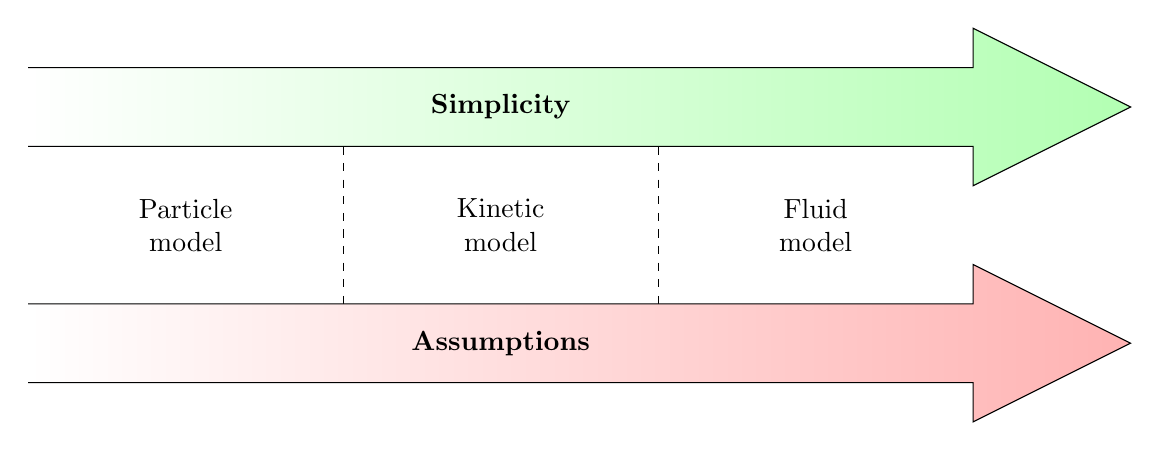
\begin{tikzpicture}[align = center, node distance = 4cm, auto]
        \node at (0, 0) {Particle \\ model};
        \node at (4, 0) {Kinetic  \\ model};
        \node at (8, 0) {Fluid    \\ model};

        \draw[dashed] (2, 1) -- (2, - 1);
        \draw[dashed] (6, 1) -- (6, - 1);
        
        \draw[left color = white, right color = green!30!white]
            (- 2, 1) -- (10, 1) -- (10, 0.5) -- (12, 1.5) -- (10, 2.5) -- (10, 2) -- (- 2, 2);
        \node at (4, 1.5) {\bf Simplicity};
        
        \draw[left color = white, right color = red!30!white]
            (- 2, - 1) -- (10, - 1) -- (10, - 0.5) -- (12, - 1.5) -- (10, - 2.5) -- (10, - 2) -- (- 2, - 2);
        \node at (4, - 1.5) {\bf Assumptions};
    \end{tikzpicture}\end{center}

    For classical single phase, electrically-neutral fluids under typical real-world conditions, these assumptions are almost wholly valid, leading to the Navier--Stokes (NS) equations. When the same steps are applied for a quasineutral plasma, one derives the magnetohydrodynamic (MHD) equations.
    
    Under typical tokamak-like conditions however, the steps required to go from the kinetic model to the fluid model do not hold nearly as well. Full fluid models like the MHD equations fail to capture highly influential ``kinetic effects'', which are necessarily present only in the full kinetic model, which are highly influential in tokamak plasma dynamics. These include:
    \begin{itemize}
        \item  Most plasma waves \BA{[Ref]}
        \item  Most plasma/kinetic instabilities \BA{[Ref]}
        \item  Landau damping/Bump-on-tail instabilities \BA{[Ref]}
        \item  Leakage \BA{[Ref]}
        \item  Kinetic structures (Beams/Double layers) \BA{[Ref]}
        \item  Anisotropic pressures \BA{[Ref]}
    \end{itemize}
    Conversely, the full kinetic equation is 6-dimensional in position/velocity phase-space, and so its direct simulation is, in most situations, computationally intractable.

    For practical purposes therefore, one requires some form of trade-off between a fully fluid and fully kinetic model. One common such technique is gyro-averaging, in the gyrokinetic model \cite{Howes_et_al_2006, Parra_Barnes_Peters_2011, Abel_et_al_2013} which has been seen to be effective in modeling many kinds of plasma turbulence \cite{McKee_et_al_2001} but can exhibit non-physical behavior over long time periods \BA{[Ref]} among other physical weaknesses \BA{[Ref]}. Some gyroaveraging shall be considered when appropriate for pseudo-particle modeling. \BA{Other examples of such models?.}
    
    In this thesis, we shall consider a coupled $\delta\!f$ low-noise correction method. To obtain this model, a derivation of the classical MHD model is presented in the following, with an analysis of the reasons for which it fails for highly kinetic tokamak plasmas.

    
    \documentclass[12pt, a4paper]{report}

\documentclass[12pt, a4paper]{report}

\documentclass[12pt, a4paper]{report}

\input{template/main.tex}

\title{\BA{Title in Progress...}}
\author{Boris Andrews}
\affil{Mathematical Institute, University of Oxford}
\date{\today}


\begin{document}
    \pagenumbering{gobble}
    \maketitle
    
    
    \begin{abstract}
        Magnetic confinement reactors---in particular tokamaks---offer one of the most promising options for achieving practical nuclear fusion, with the potential to provide virtually limitless, clean energy. The theoretical and numerical modeling of tokamak plasmas is simultaneously an essential component of effective reactor design, and a great research barrier. Tokamak operational conditions exhibit comparatively low Knudsen numbers. Kinetic effects, including kinetic waves and instabilities, Landau damping, bump-on-tail instabilities and more, are therefore highly influential in tokamak plasma dynamics. Purely fluid models are inherently incapable of capturing these effects, whereas the high dimensionality in purely kinetic models render them practically intractable for most relevant purposes.

        We consider a $\delta\!f$ decomposition model, with a macroscopic fluid background and microscopic kinetic correction, both fully coupled to each other. A similar manner of discretization is proposed to that used in the recent \texttt{STRUPHY} code \cite{Holderied_Possanner_Wang_2021, Holderied_2022, Li_et_al_2023} with a finite-element model for the background and a pseudo-particle/PiC model for the correction.

        The fluid background satisfies the full, non-linear, resistive, compressible, Hall MHD equations. \cite{Laakmann_Hu_Farrell_2022} introduces finite-element(-in-space) implicit timesteppers for the incompressible analogue to this system with structure-preserving (SP) properties in the ideal case, alongside parameter-robust preconditioners. We show that these timesteppers can derive from a finite-element-in-time (FET) (and finite-element-in-space) interpretation. The benefits of this reformulation are discussed, including the derivation of timesteppers that are higher order in time, and the quantifiable dissipative SP properties in the non-ideal, resistive case.
        
        We discuss possible options for extending this FET approach to timesteppers for the compressible case.

        The kinetic corrections satisfy linearized Boltzmann equations. Using a Lénard--Bernstein collision operator, these take Fokker--Planck-like forms \cite{Fokker_1914, Planck_1917} wherein pseudo-particles in the numerical model obey the neoclassical transport equations, with particle-independent Brownian drift terms. This offers a rigorous methodology for incorporating collisions into the particle transport model, without coupling the equations of motions for each particle.
        
        Works by Chen, Chacón et al. \cite{Chen_Chacón_Barnes_2011, Chacón_Chen_Barnes_2013, Chen_Chacón_2014, Chen_Chacón_2015} have developed structure-preserving particle pushers for neoclassical transport in the Vlasov equations, derived from Crank--Nicolson integrators. We show these too can can derive from a FET interpretation, similarly offering potential extensions to higher-order-in-time particle pushers. The FET formulation is used also to consider how the stochastic drift terms can be incorporated into the pushers. Stochastic gyrokinetic expansions are also discussed.

        Different options for the numerical implementation of these schemes are considered.

        Due to the efficacy of FET in the development of SP timesteppers for both the fluid and kinetic component, we hope this approach will prove effective in the future for developing SP timesteppers for the full hybrid model. We hope this will give us the opportunity to incorporate previously inaccessible kinetic effects into the highly effective, modern, finite-element MHD models.
    \end{abstract}
    
    
    \newpage
    \tableofcontents
    
    
    \newpage
    \pagenumbering{arabic}
    %\linenumbers\renewcommand\thelinenumber{\color{black!50}\arabic{linenumber}}
            \input{0 - introduction/main.tex}
        \part{Research}
            \input{1 - low-noise PiC models/main.tex}
            \input{2 - kinetic component/main.tex}
            \input{3 - fluid component/main.tex}
            \input{4 - numerical implementation/main.tex}
        \part{Project Overview}
            \input{5 - research plan/main.tex}
            \input{6 - summary/main.tex}
    
    
    %\section{}
    \newpage
    \pagenumbering{gobble}
        \printbibliography


    \newpage
    \pagenumbering{roman}
    \appendix
        \part{Appendices}
            \input{8 - Hilbert complexes/main.tex}
            \input{9 - weak conservation proofs/main.tex}
\end{document}


\title{\BA{Title in Progress...}}
\author{Boris Andrews}
\affil{Mathematical Institute, University of Oxford}
\date{\today}


\begin{document}
    \pagenumbering{gobble}
    \maketitle
    
    
    \begin{abstract}
        Magnetic confinement reactors---in particular tokamaks---offer one of the most promising options for achieving practical nuclear fusion, with the potential to provide virtually limitless, clean energy. The theoretical and numerical modeling of tokamak plasmas is simultaneously an essential component of effective reactor design, and a great research barrier. Tokamak operational conditions exhibit comparatively low Knudsen numbers. Kinetic effects, including kinetic waves and instabilities, Landau damping, bump-on-tail instabilities and more, are therefore highly influential in tokamak plasma dynamics. Purely fluid models are inherently incapable of capturing these effects, whereas the high dimensionality in purely kinetic models render them practically intractable for most relevant purposes.

        We consider a $\delta\!f$ decomposition model, with a macroscopic fluid background and microscopic kinetic correction, both fully coupled to each other. A similar manner of discretization is proposed to that used in the recent \texttt{STRUPHY} code \cite{Holderied_Possanner_Wang_2021, Holderied_2022, Li_et_al_2023} with a finite-element model for the background and a pseudo-particle/PiC model for the correction.

        The fluid background satisfies the full, non-linear, resistive, compressible, Hall MHD equations. \cite{Laakmann_Hu_Farrell_2022} introduces finite-element(-in-space) implicit timesteppers for the incompressible analogue to this system with structure-preserving (SP) properties in the ideal case, alongside parameter-robust preconditioners. We show that these timesteppers can derive from a finite-element-in-time (FET) (and finite-element-in-space) interpretation. The benefits of this reformulation are discussed, including the derivation of timesteppers that are higher order in time, and the quantifiable dissipative SP properties in the non-ideal, resistive case.
        
        We discuss possible options for extending this FET approach to timesteppers for the compressible case.

        The kinetic corrections satisfy linearized Boltzmann equations. Using a Lénard--Bernstein collision operator, these take Fokker--Planck-like forms \cite{Fokker_1914, Planck_1917} wherein pseudo-particles in the numerical model obey the neoclassical transport equations, with particle-independent Brownian drift terms. This offers a rigorous methodology for incorporating collisions into the particle transport model, without coupling the equations of motions for each particle.
        
        Works by Chen, Chacón et al. \cite{Chen_Chacón_Barnes_2011, Chacón_Chen_Barnes_2013, Chen_Chacón_2014, Chen_Chacón_2015} have developed structure-preserving particle pushers for neoclassical transport in the Vlasov equations, derived from Crank--Nicolson integrators. We show these too can can derive from a FET interpretation, similarly offering potential extensions to higher-order-in-time particle pushers. The FET formulation is used also to consider how the stochastic drift terms can be incorporated into the pushers. Stochastic gyrokinetic expansions are also discussed.

        Different options for the numerical implementation of these schemes are considered.

        Due to the efficacy of FET in the development of SP timesteppers for both the fluid and kinetic component, we hope this approach will prove effective in the future for developing SP timesteppers for the full hybrid model. We hope this will give us the opportunity to incorporate previously inaccessible kinetic effects into the highly effective, modern, finite-element MHD models.
    \end{abstract}
    
    
    \newpage
    \tableofcontents
    
    
    \newpage
    \pagenumbering{arabic}
    %\linenumbers\renewcommand\thelinenumber{\color{black!50}\arabic{linenumber}}
            \documentclass[12pt, a4paper]{report}

\input{template/main.tex}

\title{\BA{Title in Progress...}}
\author{Boris Andrews}
\affil{Mathematical Institute, University of Oxford}
\date{\today}


\begin{document}
    \pagenumbering{gobble}
    \maketitle
    
    
    \begin{abstract}
        Magnetic confinement reactors---in particular tokamaks---offer one of the most promising options for achieving practical nuclear fusion, with the potential to provide virtually limitless, clean energy. The theoretical and numerical modeling of tokamak plasmas is simultaneously an essential component of effective reactor design, and a great research barrier. Tokamak operational conditions exhibit comparatively low Knudsen numbers. Kinetic effects, including kinetic waves and instabilities, Landau damping, bump-on-tail instabilities and more, are therefore highly influential in tokamak plasma dynamics. Purely fluid models are inherently incapable of capturing these effects, whereas the high dimensionality in purely kinetic models render them practically intractable for most relevant purposes.

        We consider a $\delta\!f$ decomposition model, with a macroscopic fluid background and microscopic kinetic correction, both fully coupled to each other. A similar manner of discretization is proposed to that used in the recent \texttt{STRUPHY} code \cite{Holderied_Possanner_Wang_2021, Holderied_2022, Li_et_al_2023} with a finite-element model for the background and a pseudo-particle/PiC model for the correction.

        The fluid background satisfies the full, non-linear, resistive, compressible, Hall MHD equations. \cite{Laakmann_Hu_Farrell_2022} introduces finite-element(-in-space) implicit timesteppers for the incompressible analogue to this system with structure-preserving (SP) properties in the ideal case, alongside parameter-robust preconditioners. We show that these timesteppers can derive from a finite-element-in-time (FET) (and finite-element-in-space) interpretation. The benefits of this reformulation are discussed, including the derivation of timesteppers that are higher order in time, and the quantifiable dissipative SP properties in the non-ideal, resistive case.
        
        We discuss possible options for extending this FET approach to timesteppers for the compressible case.

        The kinetic corrections satisfy linearized Boltzmann equations. Using a Lénard--Bernstein collision operator, these take Fokker--Planck-like forms \cite{Fokker_1914, Planck_1917} wherein pseudo-particles in the numerical model obey the neoclassical transport equations, with particle-independent Brownian drift terms. This offers a rigorous methodology for incorporating collisions into the particle transport model, without coupling the equations of motions for each particle.
        
        Works by Chen, Chacón et al. \cite{Chen_Chacón_Barnes_2011, Chacón_Chen_Barnes_2013, Chen_Chacón_2014, Chen_Chacón_2015} have developed structure-preserving particle pushers for neoclassical transport in the Vlasov equations, derived from Crank--Nicolson integrators. We show these too can can derive from a FET interpretation, similarly offering potential extensions to higher-order-in-time particle pushers. The FET formulation is used also to consider how the stochastic drift terms can be incorporated into the pushers. Stochastic gyrokinetic expansions are also discussed.

        Different options for the numerical implementation of these schemes are considered.

        Due to the efficacy of FET in the development of SP timesteppers for both the fluid and kinetic component, we hope this approach will prove effective in the future for developing SP timesteppers for the full hybrid model. We hope this will give us the opportunity to incorporate previously inaccessible kinetic effects into the highly effective, modern, finite-element MHD models.
    \end{abstract}
    
    
    \newpage
    \tableofcontents
    
    
    \newpage
    \pagenumbering{arabic}
    %\linenumbers\renewcommand\thelinenumber{\color{black!50}\arabic{linenumber}}
            \input{0 - introduction/main.tex}
        \part{Research}
            \input{1 - low-noise PiC models/main.tex}
            \input{2 - kinetic component/main.tex}
            \input{3 - fluid component/main.tex}
            \input{4 - numerical implementation/main.tex}
        \part{Project Overview}
            \input{5 - research plan/main.tex}
            \input{6 - summary/main.tex}
    
    
    %\section{}
    \newpage
    \pagenumbering{gobble}
        \printbibliography


    \newpage
    \pagenumbering{roman}
    \appendix
        \part{Appendices}
            \input{8 - Hilbert complexes/main.tex}
            \input{9 - weak conservation proofs/main.tex}
\end{document}

        \part{Research}
            \documentclass[12pt, a4paper]{report}

\input{template/main.tex}

\title{\BA{Title in Progress...}}
\author{Boris Andrews}
\affil{Mathematical Institute, University of Oxford}
\date{\today}


\begin{document}
    \pagenumbering{gobble}
    \maketitle
    
    
    \begin{abstract}
        Magnetic confinement reactors---in particular tokamaks---offer one of the most promising options for achieving practical nuclear fusion, with the potential to provide virtually limitless, clean energy. The theoretical and numerical modeling of tokamak plasmas is simultaneously an essential component of effective reactor design, and a great research barrier. Tokamak operational conditions exhibit comparatively low Knudsen numbers. Kinetic effects, including kinetic waves and instabilities, Landau damping, bump-on-tail instabilities and more, are therefore highly influential in tokamak plasma dynamics. Purely fluid models are inherently incapable of capturing these effects, whereas the high dimensionality in purely kinetic models render them practically intractable for most relevant purposes.

        We consider a $\delta\!f$ decomposition model, with a macroscopic fluid background and microscopic kinetic correction, both fully coupled to each other. A similar manner of discretization is proposed to that used in the recent \texttt{STRUPHY} code \cite{Holderied_Possanner_Wang_2021, Holderied_2022, Li_et_al_2023} with a finite-element model for the background and a pseudo-particle/PiC model for the correction.

        The fluid background satisfies the full, non-linear, resistive, compressible, Hall MHD equations. \cite{Laakmann_Hu_Farrell_2022} introduces finite-element(-in-space) implicit timesteppers for the incompressible analogue to this system with structure-preserving (SP) properties in the ideal case, alongside parameter-robust preconditioners. We show that these timesteppers can derive from a finite-element-in-time (FET) (and finite-element-in-space) interpretation. The benefits of this reformulation are discussed, including the derivation of timesteppers that are higher order in time, and the quantifiable dissipative SP properties in the non-ideal, resistive case.
        
        We discuss possible options for extending this FET approach to timesteppers for the compressible case.

        The kinetic corrections satisfy linearized Boltzmann equations. Using a Lénard--Bernstein collision operator, these take Fokker--Planck-like forms \cite{Fokker_1914, Planck_1917} wherein pseudo-particles in the numerical model obey the neoclassical transport equations, with particle-independent Brownian drift terms. This offers a rigorous methodology for incorporating collisions into the particle transport model, without coupling the equations of motions for each particle.
        
        Works by Chen, Chacón et al. \cite{Chen_Chacón_Barnes_2011, Chacón_Chen_Barnes_2013, Chen_Chacón_2014, Chen_Chacón_2015} have developed structure-preserving particle pushers for neoclassical transport in the Vlasov equations, derived from Crank--Nicolson integrators. We show these too can can derive from a FET interpretation, similarly offering potential extensions to higher-order-in-time particle pushers. The FET formulation is used also to consider how the stochastic drift terms can be incorporated into the pushers. Stochastic gyrokinetic expansions are also discussed.

        Different options for the numerical implementation of these schemes are considered.

        Due to the efficacy of FET in the development of SP timesteppers for both the fluid and kinetic component, we hope this approach will prove effective in the future for developing SP timesteppers for the full hybrid model. We hope this will give us the opportunity to incorporate previously inaccessible kinetic effects into the highly effective, modern, finite-element MHD models.
    \end{abstract}
    
    
    \newpage
    \tableofcontents
    
    
    \newpage
    \pagenumbering{arabic}
    %\linenumbers\renewcommand\thelinenumber{\color{black!50}\arabic{linenumber}}
            \input{0 - introduction/main.tex}
        \part{Research}
            \input{1 - low-noise PiC models/main.tex}
            \input{2 - kinetic component/main.tex}
            \input{3 - fluid component/main.tex}
            \input{4 - numerical implementation/main.tex}
        \part{Project Overview}
            \input{5 - research plan/main.tex}
            \input{6 - summary/main.tex}
    
    
    %\section{}
    \newpage
    \pagenumbering{gobble}
        \printbibliography


    \newpage
    \pagenumbering{roman}
    \appendix
        \part{Appendices}
            \input{8 - Hilbert complexes/main.tex}
            \input{9 - weak conservation proofs/main.tex}
\end{document}

            \documentclass[12pt, a4paper]{report}

\input{template/main.tex}

\title{\BA{Title in Progress...}}
\author{Boris Andrews}
\affil{Mathematical Institute, University of Oxford}
\date{\today}


\begin{document}
    \pagenumbering{gobble}
    \maketitle
    
    
    \begin{abstract}
        Magnetic confinement reactors---in particular tokamaks---offer one of the most promising options for achieving practical nuclear fusion, with the potential to provide virtually limitless, clean energy. The theoretical and numerical modeling of tokamak plasmas is simultaneously an essential component of effective reactor design, and a great research barrier. Tokamak operational conditions exhibit comparatively low Knudsen numbers. Kinetic effects, including kinetic waves and instabilities, Landau damping, bump-on-tail instabilities and more, are therefore highly influential in tokamak plasma dynamics. Purely fluid models are inherently incapable of capturing these effects, whereas the high dimensionality in purely kinetic models render them practically intractable for most relevant purposes.

        We consider a $\delta\!f$ decomposition model, with a macroscopic fluid background and microscopic kinetic correction, both fully coupled to each other. A similar manner of discretization is proposed to that used in the recent \texttt{STRUPHY} code \cite{Holderied_Possanner_Wang_2021, Holderied_2022, Li_et_al_2023} with a finite-element model for the background and a pseudo-particle/PiC model for the correction.

        The fluid background satisfies the full, non-linear, resistive, compressible, Hall MHD equations. \cite{Laakmann_Hu_Farrell_2022} introduces finite-element(-in-space) implicit timesteppers for the incompressible analogue to this system with structure-preserving (SP) properties in the ideal case, alongside parameter-robust preconditioners. We show that these timesteppers can derive from a finite-element-in-time (FET) (and finite-element-in-space) interpretation. The benefits of this reformulation are discussed, including the derivation of timesteppers that are higher order in time, and the quantifiable dissipative SP properties in the non-ideal, resistive case.
        
        We discuss possible options for extending this FET approach to timesteppers for the compressible case.

        The kinetic corrections satisfy linearized Boltzmann equations. Using a Lénard--Bernstein collision operator, these take Fokker--Planck-like forms \cite{Fokker_1914, Planck_1917} wherein pseudo-particles in the numerical model obey the neoclassical transport equations, with particle-independent Brownian drift terms. This offers a rigorous methodology for incorporating collisions into the particle transport model, without coupling the equations of motions for each particle.
        
        Works by Chen, Chacón et al. \cite{Chen_Chacón_Barnes_2011, Chacón_Chen_Barnes_2013, Chen_Chacón_2014, Chen_Chacón_2015} have developed structure-preserving particle pushers for neoclassical transport in the Vlasov equations, derived from Crank--Nicolson integrators. We show these too can can derive from a FET interpretation, similarly offering potential extensions to higher-order-in-time particle pushers. The FET formulation is used also to consider how the stochastic drift terms can be incorporated into the pushers. Stochastic gyrokinetic expansions are also discussed.

        Different options for the numerical implementation of these schemes are considered.

        Due to the efficacy of FET in the development of SP timesteppers for both the fluid and kinetic component, we hope this approach will prove effective in the future for developing SP timesteppers for the full hybrid model. We hope this will give us the opportunity to incorporate previously inaccessible kinetic effects into the highly effective, modern, finite-element MHD models.
    \end{abstract}
    
    
    \newpage
    \tableofcontents
    
    
    \newpage
    \pagenumbering{arabic}
    %\linenumbers\renewcommand\thelinenumber{\color{black!50}\arabic{linenumber}}
            \input{0 - introduction/main.tex}
        \part{Research}
            \input{1 - low-noise PiC models/main.tex}
            \input{2 - kinetic component/main.tex}
            \input{3 - fluid component/main.tex}
            \input{4 - numerical implementation/main.tex}
        \part{Project Overview}
            \input{5 - research plan/main.tex}
            \input{6 - summary/main.tex}
    
    
    %\section{}
    \newpage
    \pagenumbering{gobble}
        \printbibliography


    \newpage
    \pagenumbering{roman}
    \appendix
        \part{Appendices}
            \input{8 - Hilbert complexes/main.tex}
            \input{9 - weak conservation proofs/main.tex}
\end{document}

            \documentclass[12pt, a4paper]{report}

\input{template/main.tex}

\title{\BA{Title in Progress...}}
\author{Boris Andrews}
\affil{Mathematical Institute, University of Oxford}
\date{\today}


\begin{document}
    \pagenumbering{gobble}
    \maketitle
    
    
    \begin{abstract}
        Magnetic confinement reactors---in particular tokamaks---offer one of the most promising options for achieving practical nuclear fusion, with the potential to provide virtually limitless, clean energy. The theoretical and numerical modeling of tokamak plasmas is simultaneously an essential component of effective reactor design, and a great research barrier. Tokamak operational conditions exhibit comparatively low Knudsen numbers. Kinetic effects, including kinetic waves and instabilities, Landau damping, bump-on-tail instabilities and more, are therefore highly influential in tokamak plasma dynamics. Purely fluid models are inherently incapable of capturing these effects, whereas the high dimensionality in purely kinetic models render them practically intractable for most relevant purposes.

        We consider a $\delta\!f$ decomposition model, with a macroscopic fluid background and microscopic kinetic correction, both fully coupled to each other. A similar manner of discretization is proposed to that used in the recent \texttt{STRUPHY} code \cite{Holderied_Possanner_Wang_2021, Holderied_2022, Li_et_al_2023} with a finite-element model for the background and a pseudo-particle/PiC model for the correction.

        The fluid background satisfies the full, non-linear, resistive, compressible, Hall MHD equations. \cite{Laakmann_Hu_Farrell_2022} introduces finite-element(-in-space) implicit timesteppers for the incompressible analogue to this system with structure-preserving (SP) properties in the ideal case, alongside parameter-robust preconditioners. We show that these timesteppers can derive from a finite-element-in-time (FET) (and finite-element-in-space) interpretation. The benefits of this reformulation are discussed, including the derivation of timesteppers that are higher order in time, and the quantifiable dissipative SP properties in the non-ideal, resistive case.
        
        We discuss possible options for extending this FET approach to timesteppers for the compressible case.

        The kinetic corrections satisfy linearized Boltzmann equations. Using a Lénard--Bernstein collision operator, these take Fokker--Planck-like forms \cite{Fokker_1914, Planck_1917} wherein pseudo-particles in the numerical model obey the neoclassical transport equations, with particle-independent Brownian drift terms. This offers a rigorous methodology for incorporating collisions into the particle transport model, without coupling the equations of motions for each particle.
        
        Works by Chen, Chacón et al. \cite{Chen_Chacón_Barnes_2011, Chacón_Chen_Barnes_2013, Chen_Chacón_2014, Chen_Chacón_2015} have developed structure-preserving particle pushers for neoclassical transport in the Vlasov equations, derived from Crank--Nicolson integrators. We show these too can can derive from a FET interpretation, similarly offering potential extensions to higher-order-in-time particle pushers. The FET formulation is used also to consider how the stochastic drift terms can be incorporated into the pushers. Stochastic gyrokinetic expansions are also discussed.

        Different options for the numerical implementation of these schemes are considered.

        Due to the efficacy of FET in the development of SP timesteppers for both the fluid and kinetic component, we hope this approach will prove effective in the future for developing SP timesteppers for the full hybrid model. We hope this will give us the opportunity to incorporate previously inaccessible kinetic effects into the highly effective, modern, finite-element MHD models.
    \end{abstract}
    
    
    \newpage
    \tableofcontents
    
    
    \newpage
    \pagenumbering{arabic}
    %\linenumbers\renewcommand\thelinenumber{\color{black!50}\arabic{linenumber}}
            \input{0 - introduction/main.tex}
        \part{Research}
            \input{1 - low-noise PiC models/main.tex}
            \input{2 - kinetic component/main.tex}
            \input{3 - fluid component/main.tex}
            \input{4 - numerical implementation/main.tex}
        \part{Project Overview}
            \input{5 - research plan/main.tex}
            \input{6 - summary/main.tex}
    
    
    %\section{}
    \newpage
    \pagenumbering{gobble}
        \printbibliography


    \newpage
    \pagenumbering{roman}
    \appendix
        \part{Appendices}
            \input{8 - Hilbert complexes/main.tex}
            \input{9 - weak conservation proofs/main.tex}
\end{document}

            \documentclass[12pt, a4paper]{report}

\input{template/main.tex}

\title{\BA{Title in Progress...}}
\author{Boris Andrews}
\affil{Mathematical Institute, University of Oxford}
\date{\today}


\begin{document}
    \pagenumbering{gobble}
    \maketitle
    
    
    \begin{abstract}
        Magnetic confinement reactors---in particular tokamaks---offer one of the most promising options for achieving practical nuclear fusion, with the potential to provide virtually limitless, clean energy. The theoretical and numerical modeling of tokamak plasmas is simultaneously an essential component of effective reactor design, and a great research barrier. Tokamak operational conditions exhibit comparatively low Knudsen numbers. Kinetic effects, including kinetic waves and instabilities, Landau damping, bump-on-tail instabilities and more, are therefore highly influential in tokamak plasma dynamics. Purely fluid models are inherently incapable of capturing these effects, whereas the high dimensionality in purely kinetic models render them practically intractable for most relevant purposes.

        We consider a $\delta\!f$ decomposition model, with a macroscopic fluid background and microscopic kinetic correction, both fully coupled to each other. A similar manner of discretization is proposed to that used in the recent \texttt{STRUPHY} code \cite{Holderied_Possanner_Wang_2021, Holderied_2022, Li_et_al_2023} with a finite-element model for the background and a pseudo-particle/PiC model for the correction.

        The fluid background satisfies the full, non-linear, resistive, compressible, Hall MHD equations. \cite{Laakmann_Hu_Farrell_2022} introduces finite-element(-in-space) implicit timesteppers for the incompressible analogue to this system with structure-preserving (SP) properties in the ideal case, alongside parameter-robust preconditioners. We show that these timesteppers can derive from a finite-element-in-time (FET) (and finite-element-in-space) interpretation. The benefits of this reformulation are discussed, including the derivation of timesteppers that are higher order in time, and the quantifiable dissipative SP properties in the non-ideal, resistive case.
        
        We discuss possible options for extending this FET approach to timesteppers for the compressible case.

        The kinetic corrections satisfy linearized Boltzmann equations. Using a Lénard--Bernstein collision operator, these take Fokker--Planck-like forms \cite{Fokker_1914, Planck_1917} wherein pseudo-particles in the numerical model obey the neoclassical transport equations, with particle-independent Brownian drift terms. This offers a rigorous methodology for incorporating collisions into the particle transport model, without coupling the equations of motions for each particle.
        
        Works by Chen, Chacón et al. \cite{Chen_Chacón_Barnes_2011, Chacón_Chen_Barnes_2013, Chen_Chacón_2014, Chen_Chacón_2015} have developed structure-preserving particle pushers for neoclassical transport in the Vlasov equations, derived from Crank--Nicolson integrators. We show these too can can derive from a FET interpretation, similarly offering potential extensions to higher-order-in-time particle pushers. The FET formulation is used also to consider how the stochastic drift terms can be incorporated into the pushers. Stochastic gyrokinetic expansions are also discussed.

        Different options for the numerical implementation of these schemes are considered.

        Due to the efficacy of FET in the development of SP timesteppers for both the fluid and kinetic component, we hope this approach will prove effective in the future for developing SP timesteppers for the full hybrid model. We hope this will give us the opportunity to incorporate previously inaccessible kinetic effects into the highly effective, modern, finite-element MHD models.
    \end{abstract}
    
    
    \newpage
    \tableofcontents
    
    
    \newpage
    \pagenumbering{arabic}
    %\linenumbers\renewcommand\thelinenumber{\color{black!50}\arabic{linenumber}}
            \input{0 - introduction/main.tex}
        \part{Research}
            \input{1 - low-noise PiC models/main.tex}
            \input{2 - kinetic component/main.tex}
            \input{3 - fluid component/main.tex}
            \input{4 - numerical implementation/main.tex}
        \part{Project Overview}
            \input{5 - research plan/main.tex}
            \input{6 - summary/main.tex}
    
    
    %\section{}
    \newpage
    \pagenumbering{gobble}
        \printbibliography


    \newpage
    \pagenumbering{roman}
    \appendix
        \part{Appendices}
            \input{8 - Hilbert complexes/main.tex}
            \input{9 - weak conservation proofs/main.tex}
\end{document}

        \part{Project Overview}
            \documentclass[12pt, a4paper]{report}

\input{template/main.tex}

\title{\BA{Title in Progress...}}
\author{Boris Andrews}
\affil{Mathematical Institute, University of Oxford}
\date{\today}


\begin{document}
    \pagenumbering{gobble}
    \maketitle
    
    
    \begin{abstract}
        Magnetic confinement reactors---in particular tokamaks---offer one of the most promising options for achieving practical nuclear fusion, with the potential to provide virtually limitless, clean energy. The theoretical and numerical modeling of tokamak plasmas is simultaneously an essential component of effective reactor design, and a great research barrier. Tokamak operational conditions exhibit comparatively low Knudsen numbers. Kinetic effects, including kinetic waves and instabilities, Landau damping, bump-on-tail instabilities and more, are therefore highly influential in tokamak plasma dynamics. Purely fluid models are inherently incapable of capturing these effects, whereas the high dimensionality in purely kinetic models render them practically intractable for most relevant purposes.

        We consider a $\delta\!f$ decomposition model, with a macroscopic fluid background and microscopic kinetic correction, both fully coupled to each other. A similar manner of discretization is proposed to that used in the recent \texttt{STRUPHY} code \cite{Holderied_Possanner_Wang_2021, Holderied_2022, Li_et_al_2023} with a finite-element model for the background and a pseudo-particle/PiC model for the correction.

        The fluid background satisfies the full, non-linear, resistive, compressible, Hall MHD equations. \cite{Laakmann_Hu_Farrell_2022} introduces finite-element(-in-space) implicit timesteppers for the incompressible analogue to this system with structure-preserving (SP) properties in the ideal case, alongside parameter-robust preconditioners. We show that these timesteppers can derive from a finite-element-in-time (FET) (and finite-element-in-space) interpretation. The benefits of this reformulation are discussed, including the derivation of timesteppers that are higher order in time, and the quantifiable dissipative SP properties in the non-ideal, resistive case.
        
        We discuss possible options for extending this FET approach to timesteppers for the compressible case.

        The kinetic corrections satisfy linearized Boltzmann equations. Using a Lénard--Bernstein collision operator, these take Fokker--Planck-like forms \cite{Fokker_1914, Planck_1917} wherein pseudo-particles in the numerical model obey the neoclassical transport equations, with particle-independent Brownian drift terms. This offers a rigorous methodology for incorporating collisions into the particle transport model, without coupling the equations of motions for each particle.
        
        Works by Chen, Chacón et al. \cite{Chen_Chacón_Barnes_2011, Chacón_Chen_Barnes_2013, Chen_Chacón_2014, Chen_Chacón_2015} have developed structure-preserving particle pushers for neoclassical transport in the Vlasov equations, derived from Crank--Nicolson integrators. We show these too can can derive from a FET interpretation, similarly offering potential extensions to higher-order-in-time particle pushers. The FET formulation is used also to consider how the stochastic drift terms can be incorporated into the pushers. Stochastic gyrokinetic expansions are also discussed.

        Different options for the numerical implementation of these schemes are considered.

        Due to the efficacy of FET in the development of SP timesteppers for both the fluid and kinetic component, we hope this approach will prove effective in the future for developing SP timesteppers for the full hybrid model. We hope this will give us the opportunity to incorporate previously inaccessible kinetic effects into the highly effective, modern, finite-element MHD models.
    \end{abstract}
    
    
    \newpage
    \tableofcontents
    
    
    \newpage
    \pagenumbering{arabic}
    %\linenumbers\renewcommand\thelinenumber{\color{black!50}\arabic{linenumber}}
            \input{0 - introduction/main.tex}
        \part{Research}
            \input{1 - low-noise PiC models/main.tex}
            \input{2 - kinetic component/main.tex}
            \input{3 - fluid component/main.tex}
            \input{4 - numerical implementation/main.tex}
        \part{Project Overview}
            \input{5 - research plan/main.tex}
            \input{6 - summary/main.tex}
    
    
    %\section{}
    \newpage
    \pagenumbering{gobble}
        \printbibliography


    \newpage
    \pagenumbering{roman}
    \appendix
        \part{Appendices}
            \input{8 - Hilbert complexes/main.tex}
            \input{9 - weak conservation proofs/main.tex}
\end{document}

            \documentclass[12pt, a4paper]{report}

\input{template/main.tex}

\title{\BA{Title in Progress...}}
\author{Boris Andrews}
\affil{Mathematical Institute, University of Oxford}
\date{\today}


\begin{document}
    \pagenumbering{gobble}
    \maketitle
    
    
    \begin{abstract}
        Magnetic confinement reactors---in particular tokamaks---offer one of the most promising options for achieving practical nuclear fusion, with the potential to provide virtually limitless, clean energy. The theoretical and numerical modeling of tokamak plasmas is simultaneously an essential component of effective reactor design, and a great research barrier. Tokamak operational conditions exhibit comparatively low Knudsen numbers. Kinetic effects, including kinetic waves and instabilities, Landau damping, bump-on-tail instabilities and more, are therefore highly influential in tokamak plasma dynamics. Purely fluid models are inherently incapable of capturing these effects, whereas the high dimensionality in purely kinetic models render them practically intractable for most relevant purposes.

        We consider a $\delta\!f$ decomposition model, with a macroscopic fluid background and microscopic kinetic correction, both fully coupled to each other. A similar manner of discretization is proposed to that used in the recent \texttt{STRUPHY} code \cite{Holderied_Possanner_Wang_2021, Holderied_2022, Li_et_al_2023} with a finite-element model for the background and a pseudo-particle/PiC model for the correction.

        The fluid background satisfies the full, non-linear, resistive, compressible, Hall MHD equations. \cite{Laakmann_Hu_Farrell_2022} introduces finite-element(-in-space) implicit timesteppers for the incompressible analogue to this system with structure-preserving (SP) properties in the ideal case, alongside parameter-robust preconditioners. We show that these timesteppers can derive from a finite-element-in-time (FET) (and finite-element-in-space) interpretation. The benefits of this reformulation are discussed, including the derivation of timesteppers that are higher order in time, and the quantifiable dissipative SP properties in the non-ideal, resistive case.
        
        We discuss possible options for extending this FET approach to timesteppers for the compressible case.

        The kinetic corrections satisfy linearized Boltzmann equations. Using a Lénard--Bernstein collision operator, these take Fokker--Planck-like forms \cite{Fokker_1914, Planck_1917} wherein pseudo-particles in the numerical model obey the neoclassical transport equations, with particle-independent Brownian drift terms. This offers a rigorous methodology for incorporating collisions into the particle transport model, without coupling the equations of motions for each particle.
        
        Works by Chen, Chacón et al. \cite{Chen_Chacón_Barnes_2011, Chacón_Chen_Barnes_2013, Chen_Chacón_2014, Chen_Chacón_2015} have developed structure-preserving particle pushers for neoclassical transport in the Vlasov equations, derived from Crank--Nicolson integrators. We show these too can can derive from a FET interpretation, similarly offering potential extensions to higher-order-in-time particle pushers. The FET formulation is used also to consider how the stochastic drift terms can be incorporated into the pushers. Stochastic gyrokinetic expansions are also discussed.

        Different options for the numerical implementation of these schemes are considered.

        Due to the efficacy of FET in the development of SP timesteppers for both the fluid and kinetic component, we hope this approach will prove effective in the future for developing SP timesteppers for the full hybrid model. We hope this will give us the opportunity to incorporate previously inaccessible kinetic effects into the highly effective, modern, finite-element MHD models.
    \end{abstract}
    
    
    \newpage
    \tableofcontents
    
    
    \newpage
    \pagenumbering{arabic}
    %\linenumbers\renewcommand\thelinenumber{\color{black!50}\arabic{linenumber}}
            \input{0 - introduction/main.tex}
        \part{Research}
            \input{1 - low-noise PiC models/main.tex}
            \input{2 - kinetic component/main.tex}
            \input{3 - fluid component/main.tex}
            \input{4 - numerical implementation/main.tex}
        \part{Project Overview}
            \input{5 - research plan/main.tex}
            \input{6 - summary/main.tex}
    
    
    %\section{}
    \newpage
    \pagenumbering{gobble}
        \printbibliography


    \newpage
    \pagenumbering{roman}
    \appendix
        \part{Appendices}
            \input{8 - Hilbert complexes/main.tex}
            \input{9 - weak conservation proofs/main.tex}
\end{document}

    
    
    %\section{}
    \newpage
    \pagenumbering{gobble}
        \printbibliography


    \newpage
    \pagenumbering{roman}
    \appendix
        \part{Appendices}
            \documentclass[12pt, a4paper]{report}

\input{template/main.tex}

\title{\BA{Title in Progress...}}
\author{Boris Andrews}
\affil{Mathematical Institute, University of Oxford}
\date{\today}


\begin{document}
    \pagenumbering{gobble}
    \maketitle
    
    
    \begin{abstract}
        Magnetic confinement reactors---in particular tokamaks---offer one of the most promising options for achieving practical nuclear fusion, with the potential to provide virtually limitless, clean energy. The theoretical and numerical modeling of tokamak plasmas is simultaneously an essential component of effective reactor design, and a great research barrier. Tokamak operational conditions exhibit comparatively low Knudsen numbers. Kinetic effects, including kinetic waves and instabilities, Landau damping, bump-on-tail instabilities and more, are therefore highly influential in tokamak plasma dynamics. Purely fluid models are inherently incapable of capturing these effects, whereas the high dimensionality in purely kinetic models render them practically intractable for most relevant purposes.

        We consider a $\delta\!f$ decomposition model, with a macroscopic fluid background and microscopic kinetic correction, both fully coupled to each other. A similar manner of discretization is proposed to that used in the recent \texttt{STRUPHY} code \cite{Holderied_Possanner_Wang_2021, Holderied_2022, Li_et_al_2023} with a finite-element model for the background and a pseudo-particle/PiC model for the correction.

        The fluid background satisfies the full, non-linear, resistive, compressible, Hall MHD equations. \cite{Laakmann_Hu_Farrell_2022} introduces finite-element(-in-space) implicit timesteppers for the incompressible analogue to this system with structure-preserving (SP) properties in the ideal case, alongside parameter-robust preconditioners. We show that these timesteppers can derive from a finite-element-in-time (FET) (and finite-element-in-space) interpretation. The benefits of this reformulation are discussed, including the derivation of timesteppers that are higher order in time, and the quantifiable dissipative SP properties in the non-ideal, resistive case.
        
        We discuss possible options for extending this FET approach to timesteppers for the compressible case.

        The kinetic corrections satisfy linearized Boltzmann equations. Using a Lénard--Bernstein collision operator, these take Fokker--Planck-like forms \cite{Fokker_1914, Planck_1917} wherein pseudo-particles in the numerical model obey the neoclassical transport equations, with particle-independent Brownian drift terms. This offers a rigorous methodology for incorporating collisions into the particle transport model, without coupling the equations of motions for each particle.
        
        Works by Chen, Chacón et al. \cite{Chen_Chacón_Barnes_2011, Chacón_Chen_Barnes_2013, Chen_Chacón_2014, Chen_Chacón_2015} have developed structure-preserving particle pushers for neoclassical transport in the Vlasov equations, derived from Crank--Nicolson integrators. We show these too can can derive from a FET interpretation, similarly offering potential extensions to higher-order-in-time particle pushers. The FET formulation is used also to consider how the stochastic drift terms can be incorporated into the pushers. Stochastic gyrokinetic expansions are also discussed.

        Different options for the numerical implementation of these schemes are considered.

        Due to the efficacy of FET in the development of SP timesteppers for both the fluid and kinetic component, we hope this approach will prove effective in the future for developing SP timesteppers for the full hybrid model. We hope this will give us the opportunity to incorporate previously inaccessible kinetic effects into the highly effective, modern, finite-element MHD models.
    \end{abstract}
    
    
    \newpage
    \tableofcontents
    
    
    \newpage
    \pagenumbering{arabic}
    %\linenumbers\renewcommand\thelinenumber{\color{black!50}\arabic{linenumber}}
            \input{0 - introduction/main.tex}
        \part{Research}
            \input{1 - low-noise PiC models/main.tex}
            \input{2 - kinetic component/main.tex}
            \input{3 - fluid component/main.tex}
            \input{4 - numerical implementation/main.tex}
        \part{Project Overview}
            \input{5 - research plan/main.tex}
            \input{6 - summary/main.tex}
    
    
    %\section{}
    \newpage
    \pagenumbering{gobble}
        \printbibliography


    \newpage
    \pagenumbering{roman}
    \appendix
        \part{Appendices}
            \input{8 - Hilbert complexes/main.tex}
            \input{9 - weak conservation proofs/main.tex}
\end{document}

            \documentclass[12pt, a4paper]{report}

\input{template/main.tex}

\title{\BA{Title in Progress...}}
\author{Boris Andrews}
\affil{Mathematical Institute, University of Oxford}
\date{\today}


\begin{document}
    \pagenumbering{gobble}
    \maketitle
    
    
    \begin{abstract}
        Magnetic confinement reactors---in particular tokamaks---offer one of the most promising options for achieving practical nuclear fusion, with the potential to provide virtually limitless, clean energy. The theoretical and numerical modeling of tokamak plasmas is simultaneously an essential component of effective reactor design, and a great research barrier. Tokamak operational conditions exhibit comparatively low Knudsen numbers. Kinetic effects, including kinetic waves and instabilities, Landau damping, bump-on-tail instabilities and more, are therefore highly influential in tokamak plasma dynamics. Purely fluid models are inherently incapable of capturing these effects, whereas the high dimensionality in purely kinetic models render them practically intractable for most relevant purposes.

        We consider a $\delta\!f$ decomposition model, with a macroscopic fluid background and microscopic kinetic correction, both fully coupled to each other. A similar manner of discretization is proposed to that used in the recent \texttt{STRUPHY} code \cite{Holderied_Possanner_Wang_2021, Holderied_2022, Li_et_al_2023} with a finite-element model for the background and a pseudo-particle/PiC model for the correction.

        The fluid background satisfies the full, non-linear, resistive, compressible, Hall MHD equations. \cite{Laakmann_Hu_Farrell_2022} introduces finite-element(-in-space) implicit timesteppers for the incompressible analogue to this system with structure-preserving (SP) properties in the ideal case, alongside parameter-robust preconditioners. We show that these timesteppers can derive from a finite-element-in-time (FET) (and finite-element-in-space) interpretation. The benefits of this reformulation are discussed, including the derivation of timesteppers that are higher order in time, and the quantifiable dissipative SP properties in the non-ideal, resistive case.
        
        We discuss possible options for extending this FET approach to timesteppers for the compressible case.

        The kinetic corrections satisfy linearized Boltzmann equations. Using a Lénard--Bernstein collision operator, these take Fokker--Planck-like forms \cite{Fokker_1914, Planck_1917} wherein pseudo-particles in the numerical model obey the neoclassical transport equations, with particle-independent Brownian drift terms. This offers a rigorous methodology for incorporating collisions into the particle transport model, without coupling the equations of motions for each particle.
        
        Works by Chen, Chacón et al. \cite{Chen_Chacón_Barnes_2011, Chacón_Chen_Barnes_2013, Chen_Chacón_2014, Chen_Chacón_2015} have developed structure-preserving particle pushers for neoclassical transport in the Vlasov equations, derived from Crank--Nicolson integrators. We show these too can can derive from a FET interpretation, similarly offering potential extensions to higher-order-in-time particle pushers. The FET formulation is used also to consider how the stochastic drift terms can be incorporated into the pushers. Stochastic gyrokinetic expansions are also discussed.

        Different options for the numerical implementation of these schemes are considered.

        Due to the efficacy of FET in the development of SP timesteppers for both the fluid and kinetic component, we hope this approach will prove effective in the future for developing SP timesteppers for the full hybrid model. We hope this will give us the opportunity to incorporate previously inaccessible kinetic effects into the highly effective, modern, finite-element MHD models.
    \end{abstract}
    
    
    \newpage
    \tableofcontents
    
    
    \newpage
    \pagenumbering{arabic}
    %\linenumbers\renewcommand\thelinenumber{\color{black!50}\arabic{linenumber}}
            \input{0 - introduction/main.tex}
        \part{Research}
            \input{1 - low-noise PiC models/main.tex}
            \input{2 - kinetic component/main.tex}
            \input{3 - fluid component/main.tex}
            \input{4 - numerical implementation/main.tex}
        \part{Project Overview}
            \input{5 - research plan/main.tex}
            \input{6 - summary/main.tex}
    
    
    %\section{}
    \newpage
    \pagenumbering{gobble}
        \printbibliography


    \newpage
    \pagenumbering{roman}
    \appendix
        \part{Appendices}
            \input{8 - Hilbert complexes/main.tex}
            \input{9 - weak conservation proofs/main.tex}
\end{document}

\end{document}


\title{\BA{Title in Progress...}}
\author{Boris Andrews}
\affil{Mathematical Institute, University of Oxford}
\date{\today}


\begin{document}
    \pagenumbering{gobble}
    \maketitle
    
    
    \begin{abstract}
        Magnetic confinement reactors---in particular tokamaks---offer one of the most promising options for achieving practical nuclear fusion, with the potential to provide virtually limitless, clean energy. The theoretical and numerical modeling of tokamak plasmas is simultaneously an essential component of effective reactor design, and a great research barrier. Tokamak operational conditions exhibit comparatively low Knudsen numbers. Kinetic effects, including kinetic waves and instabilities, Landau damping, bump-on-tail instabilities and more, are therefore highly influential in tokamak plasma dynamics. Purely fluid models are inherently incapable of capturing these effects, whereas the high dimensionality in purely kinetic models render them practically intractable for most relevant purposes.

        We consider a $\delta\!f$ decomposition model, with a macroscopic fluid background and microscopic kinetic correction, both fully coupled to each other. A similar manner of discretization is proposed to that used in the recent \texttt{STRUPHY} code \cite{Holderied_Possanner_Wang_2021, Holderied_2022, Li_et_al_2023} with a finite-element model for the background and a pseudo-particle/PiC model for the correction.

        The fluid background satisfies the full, non-linear, resistive, compressible, Hall MHD equations. \cite{Laakmann_Hu_Farrell_2022} introduces finite-element(-in-space) implicit timesteppers for the incompressible analogue to this system with structure-preserving (SP) properties in the ideal case, alongside parameter-robust preconditioners. We show that these timesteppers can derive from a finite-element-in-time (FET) (and finite-element-in-space) interpretation. The benefits of this reformulation are discussed, including the derivation of timesteppers that are higher order in time, and the quantifiable dissipative SP properties in the non-ideal, resistive case.
        
        We discuss possible options for extending this FET approach to timesteppers for the compressible case.

        The kinetic corrections satisfy linearized Boltzmann equations. Using a Lénard--Bernstein collision operator, these take Fokker--Planck-like forms \cite{Fokker_1914, Planck_1917} wherein pseudo-particles in the numerical model obey the neoclassical transport equations, with particle-independent Brownian drift terms. This offers a rigorous methodology for incorporating collisions into the particle transport model, without coupling the equations of motions for each particle.
        
        Works by Chen, Chacón et al. \cite{Chen_Chacón_Barnes_2011, Chacón_Chen_Barnes_2013, Chen_Chacón_2014, Chen_Chacón_2015} have developed structure-preserving particle pushers for neoclassical transport in the Vlasov equations, derived from Crank--Nicolson integrators. We show these too can can derive from a FET interpretation, similarly offering potential extensions to higher-order-in-time particle pushers. The FET formulation is used also to consider how the stochastic drift terms can be incorporated into the pushers. Stochastic gyrokinetic expansions are also discussed.

        Different options for the numerical implementation of these schemes are considered.

        Due to the efficacy of FET in the development of SP timesteppers for both the fluid and kinetic component, we hope this approach will prove effective in the future for developing SP timesteppers for the full hybrid model. We hope this will give us the opportunity to incorporate previously inaccessible kinetic effects into the highly effective, modern, finite-element MHD models.
    \end{abstract}
    
    
    \newpage
    \tableofcontents
    
    
    \newpage
    \pagenumbering{arabic}
    %\linenumbers\renewcommand\thelinenumber{\color{black!50}\arabic{linenumber}}
            \documentclass[12pt, a4paper]{report}

\documentclass[12pt, a4paper]{report}

\input{template/main.tex}

\title{\BA{Title in Progress...}}
\author{Boris Andrews}
\affil{Mathematical Institute, University of Oxford}
\date{\today}


\begin{document}
    \pagenumbering{gobble}
    \maketitle
    
    
    \begin{abstract}
        Magnetic confinement reactors---in particular tokamaks---offer one of the most promising options for achieving practical nuclear fusion, with the potential to provide virtually limitless, clean energy. The theoretical and numerical modeling of tokamak plasmas is simultaneously an essential component of effective reactor design, and a great research barrier. Tokamak operational conditions exhibit comparatively low Knudsen numbers. Kinetic effects, including kinetic waves and instabilities, Landau damping, bump-on-tail instabilities and more, are therefore highly influential in tokamak plasma dynamics. Purely fluid models are inherently incapable of capturing these effects, whereas the high dimensionality in purely kinetic models render them practically intractable for most relevant purposes.

        We consider a $\delta\!f$ decomposition model, with a macroscopic fluid background and microscopic kinetic correction, both fully coupled to each other. A similar manner of discretization is proposed to that used in the recent \texttt{STRUPHY} code \cite{Holderied_Possanner_Wang_2021, Holderied_2022, Li_et_al_2023} with a finite-element model for the background and a pseudo-particle/PiC model for the correction.

        The fluid background satisfies the full, non-linear, resistive, compressible, Hall MHD equations. \cite{Laakmann_Hu_Farrell_2022} introduces finite-element(-in-space) implicit timesteppers for the incompressible analogue to this system with structure-preserving (SP) properties in the ideal case, alongside parameter-robust preconditioners. We show that these timesteppers can derive from a finite-element-in-time (FET) (and finite-element-in-space) interpretation. The benefits of this reformulation are discussed, including the derivation of timesteppers that are higher order in time, and the quantifiable dissipative SP properties in the non-ideal, resistive case.
        
        We discuss possible options for extending this FET approach to timesteppers for the compressible case.

        The kinetic corrections satisfy linearized Boltzmann equations. Using a Lénard--Bernstein collision operator, these take Fokker--Planck-like forms \cite{Fokker_1914, Planck_1917} wherein pseudo-particles in the numerical model obey the neoclassical transport equations, with particle-independent Brownian drift terms. This offers a rigorous methodology for incorporating collisions into the particle transport model, without coupling the equations of motions for each particle.
        
        Works by Chen, Chacón et al. \cite{Chen_Chacón_Barnes_2011, Chacón_Chen_Barnes_2013, Chen_Chacón_2014, Chen_Chacón_2015} have developed structure-preserving particle pushers for neoclassical transport in the Vlasov equations, derived from Crank--Nicolson integrators. We show these too can can derive from a FET interpretation, similarly offering potential extensions to higher-order-in-time particle pushers. The FET formulation is used also to consider how the stochastic drift terms can be incorporated into the pushers. Stochastic gyrokinetic expansions are also discussed.

        Different options for the numerical implementation of these schemes are considered.

        Due to the efficacy of FET in the development of SP timesteppers for both the fluid and kinetic component, we hope this approach will prove effective in the future for developing SP timesteppers for the full hybrid model. We hope this will give us the opportunity to incorporate previously inaccessible kinetic effects into the highly effective, modern, finite-element MHD models.
    \end{abstract}
    
    
    \newpage
    \tableofcontents
    
    
    \newpage
    \pagenumbering{arabic}
    %\linenumbers\renewcommand\thelinenumber{\color{black!50}\arabic{linenumber}}
            \input{0 - introduction/main.tex}
        \part{Research}
            \input{1 - low-noise PiC models/main.tex}
            \input{2 - kinetic component/main.tex}
            \input{3 - fluid component/main.tex}
            \input{4 - numerical implementation/main.tex}
        \part{Project Overview}
            \input{5 - research plan/main.tex}
            \input{6 - summary/main.tex}
    
    
    %\section{}
    \newpage
    \pagenumbering{gobble}
        \printbibliography


    \newpage
    \pagenumbering{roman}
    \appendix
        \part{Appendices}
            \input{8 - Hilbert complexes/main.tex}
            \input{9 - weak conservation proofs/main.tex}
\end{document}


\title{\BA{Title in Progress...}}
\author{Boris Andrews}
\affil{Mathematical Institute, University of Oxford}
\date{\today}


\begin{document}
    \pagenumbering{gobble}
    \maketitle
    
    
    \begin{abstract}
        Magnetic confinement reactors---in particular tokamaks---offer one of the most promising options for achieving practical nuclear fusion, with the potential to provide virtually limitless, clean energy. The theoretical and numerical modeling of tokamak plasmas is simultaneously an essential component of effective reactor design, and a great research barrier. Tokamak operational conditions exhibit comparatively low Knudsen numbers. Kinetic effects, including kinetic waves and instabilities, Landau damping, bump-on-tail instabilities and more, are therefore highly influential in tokamak plasma dynamics. Purely fluid models are inherently incapable of capturing these effects, whereas the high dimensionality in purely kinetic models render them practically intractable for most relevant purposes.

        We consider a $\delta\!f$ decomposition model, with a macroscopic fluid background and microscopic kinetic correction, both fully coupled to each other. A similar manner of discretization is proposed to that used in the recent \texttt{STRUPHY} code \cite{Holderied_Possanner_Wang_2021, Holderied_2022, Li_et_al_2023} with a finite-element model for the background and a pseudo-particle/PiC model for the correction.

        The fluid background satisfies the full, non-linear, resistive, compressible, Hall MHD equations. \cite{Laakmann_Hu_Farrell_2022} introduces finite-element(-in-space) implicit timesteppers for the incompressible analogue to this system with structure-preserving (SP) properties in the ideal case, alongside parameter-robust preconditioners. We show that these timesteppers can derive from a finite-element-in-time (FET) (and finite-element-in-space) interpretation. The benefits of this reformulation are discussed, including the derivation of timesteppers that are higher order in time, and the quantifiable dissipative SP properties in the non-ideal, resistive case.
        
        We discuss possible options for extending this FET approach to timesteppers for the compressible case.

        The kinetic corrections satisfy linearized Boltzmann equations. Using a Lénard--Bernstein collision operator, these take Fokker--Planck-like forms \cite{Fokker_1914, Planck_1917} wherein pseudo-particles in the numerical model obey the neoclassical transport equations, with particle-independent Brownian drift terms. This offers a rigorous methodology for incorporating collisions into the particle transport model, without coupling the equations of motions for each particle.
        
        Works by Chen, Chacón et al. \cite{Chen_Chacón_Barnes_2011, Chacón_Chen_Barnes_2013, Chen_Chacón_2014, Chen_Chacón_2015} have developed structure-preserving particle pushers for neoclassical transport in the Vlasov equations, derived from Crank--Nicolson integrators. We show these too can can derive from a FET interpretation, similarly offering potential extensions to higher-order-in-time particle pushers. The FET formulation is used also to consider how the stochastic drift terms can be incorporated into the pushers. Stochastic gyrokinetic expansions are also discussed.

        Different options for the numerical implementation of these schemes are considered.

        Due to the efficacy of FET in the development of SP timesteppers for both the fluid and kinetic component, we hope this approach will prove effective in the future for developing SP timesteppers for the full hybrid model. We hope this will give us the opportunity to incorporate previously inaccessible kinetic effects into the highly effective, modern, finite-element MHD models.
    \end{abstract}
    
    
    \newpage
    \tableofcontents
    
    
    \newpage
    \pagenumbering{arabic}
    %\linenumbers\renewcommand\thelinenumber{\color{black!50}\arabic{linenumber}}
            \documentclass[12pt, a4paper]{report}

\input{template/main.tex}

\title{\BA{Title in Progress...}}
\author{Boris Andrews}
\affil{Mathematical Institute, University of Oxford}
\date{\today}


\begin{document}
    \pagenumbering{gobble}
    \maketitle
    
    
    \begin{abstract}
        Magnetic confinement reactors---in particular tokamaks---offer one of the most promising options for achieving practical nuclear fusion, with the potential to provide virtually limitless, clean energy. The theoretical and numerical modeling of tokamak plasmas is simultaneously an essential component of effective reactor design, and a great research barrier. Tokamak operational conditions exhibit comparatively low Knudsen numbers. Kinetic effects, including kinetic waves and instabilities, Landau damping, bump-on-tail instabilities and more, are therefore highly influential in tokamak plasma dynamics. Purely fluid models are inherently incapable of capturing these effects, whereas the high dimensionality in purely kinetic models render them practically intractable for most relevant purposes.

        We consider a $\delta\!f$ decomposition model, with a macroscopic fluid background and microscopic kinetic correction, both fully coupled to each other. A similar manner of discretization is proposed to that used in the recent \texttt{STRUPHY} code \cite{Holderied_Possanner_Wang_2021, Holderied_2022, Li_et_al_2023} with a finite-element model for the background and a pseudo-particle/PiC model for the correction.

        The fluid background satisfies the full, non-linear, resistive, compressible, Hall MHD equations. \cite{Laakmann_Hu_Farrell_2022} introduces finite-element(-in-space) implicit timesteppers for the incompressible analogue to this system with structure-preserving (SP) properties in the ideal case, alongside parameter-robust preconditioners. We show that these timesteppers can derive from a finite-element-in-time (FET) (and finite-element-in-space) interpretation. The benefits of this reformulation are discussed, including the derivation of timesteppers that are higher order in time, and the quantifiable dissipative SP properties in the non-ideal, resistive case.
        
        We discuss possible options for extending this FET approach to timesteppers for the compressible case.

        The kinetic corrections satisfy linearized Boltzmann equations. Using a Lénard--Bernstein collision operator, these take Fokker--Planck-like forms \cite{Fokker_1914, Planck_1917} wherein pseudo-particles in the numerical model obey the neoclassical transport equations, with particle-independent Brownian drift terms. This offers a rigorous methodology for incorporating collisions into the particle transport model, without coupling the equations of motions for each particle.
        
        Works by Chen, Chacón et al. \cite{Chen_Chacón_Barnes_2011, Chacón_Chen_Barnes_2013, Chen_Chacón_2014, Chen_Chacón_2015} have developed structure-preserving particle pushers for neoclassical transport in the Vlasov equations, derived from Crank--Nicolson integrators. We show these too can can derive from a FET interpretation, similarly offering potential extensions to higher-order-in-time particle pushers. The FET formulation is used also to consider how the stochastic drift terms can be incorporated into the pushers. Stochastic gyrokinetic expansions are also discussed.

        Different options for the numerical implementation of these schemes are considered.

        Due to the efficacy of FET in the development of SP timesteppers for both the fluid and kinetic component, we hope this approach will prove effective in the future for developing SP timesteppers for the full hybrid model. We hope this will give us the opportunity to incorporate previously inaccessible kinetic effects into the highly effective, modern, finite-element MHD models.
    \end{abstract}
    
    
    \newpage
    \tableofcontents
    
    
    \newpage
    \pagenumbering{arabic}
    %\linenumbers\renewcommand\thelinenumber{\color{black!50}\arabic{linenumber}}
            \input{0 - introduction/main.tex}
        \part{Research}
            \input{1 - low-noise PiC models/main.tex}
            \input{2 - kinetic component/main.tex}
            \input{3 - fluid component/main.tex}
            \input{4 - numerical implementation/main.tex}
        \part{Project Overview}
            \input{5 - research plan/main.tex}
            \input{6 - summary/main.tex}
    
    
    %\section{}
    \newpage
    \pagenumbering{gobble}
        \printbibliography


    \newpage
    \pagenumbering{roman}
    \appendix
        \part{Appendices}
            \input{8 - Hilbert complexes/main.tex}
            \input{9 - weak conservation proofs/main.tex}
\end{document}

        \part{Research}
            \documentclass[12pt, a4paper]{report}

\input{template/main.tex}

\title{\BA{Title in Progress...}}
\author{Boris Andrews}
\affil{Mathematical Institute, University of Oxford}
\date{\today}


\begin{document}
    \pagenumbering{gobble}
    \maketitle
    
    
    \begin{abstract}
        Magnetic confinement reactors---in particular tokamaks---offer one of the most promising options for achieving practical nuclear fusion, with the potential to provide virtually limitless, clean energy. The theoretical and numerical modeling of tokamak plasmas is simultaneously an essential component of effective reactor design, and a great research barrier. Tokamak operational conditions exhibit comparatively low Knudsen numbers. Kinetic effects, including kinetic waves and instabilities, Landau damping, bump-on-tail instabilities and more, are therefore highly influential in tokamak plasma dynamics. Purely fluid models are inherently incapable of capturing these effects, whereas the high dimensionality in purely kinetic models render them practically intractable for most relevant purposes.

        We consider a $\delta\!f$ decomposition model, with a macroscopic fluid background and microscopic kinetic correction, both fully coupled to each other. A similar manner of discretization is proposed to that used in the recent \texttt{STRUPHY} code \cite{Holderied_Possanner_Wang_2021, Holderied_2022, Li_et_al_2023} with a finite-element model for the background and a pseudo-particle/PiC model for the correction.

        The fluid background satisfies the full, non-linear, resistive, compressible, Hall MHD equations. \cite{Laakmann_Hu_Farrell_2022} introduces finite-element(-in-space) implicit timesteppers for the incompressible analogue to this system with structure-preserving (SP) properties in the ideal case, alongside parameter-robust preconditioners. We show that these timesteppers can derive from a finite-element-in-time (FET) (and finite-element-in-space) interpretation. The benefits of this reformulation are discussed, including the derivation of timesteppers that are higher order in time, and the quantifiable dissipative SP properties in the non-ideal, resistive case.
        
        We discuss possible options for extending this FET approach to timesteppers for the compressible case.

        The kinetic corrections satisfy linearized Boltzmann equations. Using a Lénard--Bernstein collision operator, these take Fokker--Planck-like forms \cite{Fokker_1914, Planck_1917} wherein pseudo-particles in the numerical model obey the neoclassical transport equations, with particle-independent Brownian drift terms. This offers a rigorous methodology for incorporating collisions into the particle transport model, without coupling the equations of motions for each particle.
        
        Works by Chen, Chacón et al. \cite{Chen_Chacón_Barnes_2011, Chacón_Chen_Barnes_2013, Chen_Chacón_2014, Chen_Chacón_2015} have developed structure-preserving particle pushers for neoclassical transport in the Vlasov equations, derived from Crank--Nicolson integrators. We show these too can can derive from a FET interpretation, similarly offering potential extensions to higher-order-in-time particle pushers. The FET formulation is used also to consider how the stochastic drift terms can be incorporated into the pushers. Stochastic gyrokinetic expansions are also discussed.

        Different options for the numerical implementation of these schemes are considered.

        Due to the efficacy of FET in the development of SP timesteppers for both the fluid and kinetic component, we hope this approach will prove effective in the future for developing SP timesteppers for the full hybrid model. We hope this will give us the opportunity to incorporate previously inaccessible kinetic effects into the highly effective, modern, finite-element MHD models.
    \end{abstract}
    
    
    \newpage
    \tableofcontents
    
    
    \newpage
    \pagenumbering{arabic}
    %\linenumbers\renewcommand\thelinenumber{\color{black!50}\arabic{linenumber}}
            \input{0 - introduction/main.tex}
        \part{Research}
            \input{1 - low-noise PiC models/main.tex}
            \input{2 - kinetic component/main.tex}
            \input{3 - fluid component/main.tex}
            \input{4 - numerical implementation/main.tex}
        \part{Project Overview}
            \input{5 - research plan/main.tex}
            \input{6 - summary/main.tex}
    
    
    %\section{}
    \newpage
    \pagenumbering{gobble}
        \printbibliography


    \newpage
    \pagenumbering{roman}
    \appendix
        \part{Appendices}
            \input{8 - Hilbert complexes/main.tex}
            \input{9 - weak conservation proofs/main.tex}
\end{document}

            \documentclass[12pt, a4paper]{report}

\input{template/main.tex}

\title{\BA{Title in Progress...}}
\author{Boris Andrews}
\affil{Mathematical Institute, University of Oxford}
\date{\today}


\begin{document}
    \pagenumbering{gobble}
    \maketitle
    
    
    \begin{abstract}
        Magnetic confinement reactors---in particular tokamaks---offer one of the most promising options for achieving practical nuclear fusion, with the potential to provide virtually limitless, clean energy. The theoretical and numerical modeling of tokamak plasmas is simultaneously an essential component of effective reactor design, and a great research barrier. Tokamak operational conditions exhibit comparatively low Knudsen numbers. Kinetic effects, including kinetic waves and instabilities, Landau damping, bump-on-tail instabilities and more, are therefore highly influential in tokamak plasma dynamics. Purely fluid models are inherently incapable of capturing these effects, whereas the high dimensionality in purely kinetic models render them practically intractable for most relevant purposes.

        We consider a $\delta\!f$ decomposition model, with a macroscopic fluid background and microscopic kinetic correction, both fully coupled to each other. A similar manner of discretization is proposed to that used in the recent \texttt{STRUPHY} code \cite{Holderied_Possanner_Wang_2021, Holderied_2022, Li_et_al_2023} with a finite-element model for the background and a pseudo-particle/PiC model for the correction.

        The fluid background satisfies the full, non-linear, resistive, compressible, Hall MHD equations. \cite{Laakmann_Hu_Farrell_2022} introduces finite-element(-in-space) implicit timesteppers for the incompressible analogue to this system with structure-preserving (SP) properties in the ideal case, alongside parameter-robust preconditioners. We show that these timesteppers can derive from a finite-element-in-time (FET) (and finite-element-in-space) interpretation. The benefits of this reformulation are discussed, including the derivation of timesteppers that are higher order in time, and the quantifiable dissipative SP properties in the non-ideal, resistive case.
        
        We discuss possible options for extending this FET approach to timesteppers for the compressible case.

        The kinetic corrections satisfy linearized Boltzmann equations. Using a Lénard--Bernstein collision operator, these take Fokker--Planck-like forms \cite{Fokker_1914, Planck_1917} wherein pseudo-particles in the numerical model obey the neoclassical transport equations, with particle-independent Brownian drift terms. This offers a rigorous methodology for incorporating collisions into the particle transport model, without coupling the equations of motions for each particle.
        
        Works by Chen, Chacón et al. \cite{Chen_Chacón_Barnes_2011, Chacón_Chen_Barnes_2013, Chen_Chacón_2014, Chen_Chacón_2015} have developed structure-preserving particle pushers for neoclassical transport in the Vlasov equations, derived from Crank--Nicolson integrators. We show these too can can derive from a FET interpretation, similarly offering potential extensions to higher-order-in-time particle pushers. The FET formulation is used also to consider how the stochastic drift terms can be incorporated into the pushers. Stochastic gyrokinetic expansions are also discussed.

        Different options for the numerical implementation of these schemes are considered.

        Due to the efficacy of FET in the development of SP timesteppers for both the fluid and kinetic component, we hope this approach will prove effective in the future for developing SP timesteppers for the full hybrid model. We hope this will give us the opportunity to incorporate previously inaccessible kinetic effects into the highly effective, modern, finite-element MHD models.
    \end{abstract}
    
    
    \newpage
    \tableofcontents
    
    
    \newpage
    \pagenumbering{arabic}
    %\linenumbers\renewcommand\thelinenumber{\color{black!50}\arabic{linenumber}}
            \input{0 - introduction/main.tex}
        \part{Research}
            \input{1 - low-noise PiC models/main.tex}
            \input{2 - kinetic component/main.tex}
            \input{3 - fluid component/main.tex}
            \input{4 - numerical implementation/main.tex}
        \part{Project Overview}
            \input{5 - research plan/main.tex}
            \input{6 - summary/main.tex}
    
    
    %\section{}
    \newpage
    \pagenumbering{gobble}
        \printbibliography


    \newpage
    \pagenumbering{roman}
    \appendix
        \part{Appendices}
            \input{8 - Hilbert complexes/main.tex}
            \input{9 - weak conservation proofs/main.tex}
\end{document}

            \documentclass[12pt, a4paper]{report}

\input{template/main.tex}

\title{\BA{Title in Progress...}}
\author{Boris Andrews}
\affil{Mathematical Institute, University of Oxford}
\date{\today}


\begin{document}
    \pagenumbering{gobble}
    \maketitle
    
    
    \begin{abstract}
        Magnetic confinement reactors---in particular tokamaks---offer one of the most promising options for achieving practical nuclear fusion, with the potential to provide virtually limitless, clean energy. The theoretical and numerical modeling of tokamak plasmas is simultaneously an essential component of effective reactor design, and a great research barrier. Tokamak operational conditions exhibit comparatively low Knudsen numbers. Kinetic effects, including kinetic waves and instabilities, Landau damping, bump-on-tail instabilities and more, are therefore highly influential in tokamak plasma dynamics. Purely fluid models are inherently incapable of capturing these effects, whereas the high dimensionality in purely kinetic models render them practically intractable for most relevant purposes.

        We consider a $\delta\!f$ decomposition model, with a macroscopic fluid background and microscopic kinetic correction, both fully coupled to each other. A similar manner of discretization is proposed to that used in the recent \texttt{STRUPHY} code \cite{Holderied_Possanner_Wang_2021, Holderied_2022, Li_et_al_2023} with a finite-element model for the background and a pseudo-particle/PiC model for the correction.

        The fluid background satisfies the full, non-linear, resistive, compressible, Hall MHD equations. \cite{Laakmann_Hu_Farrell_2022} introduces finite-element(-in-space) implicit timesteppers for the incompressible analogue to this system with structure-preserving (SP) properties in the ideal case, alongside parameter-robust preconditioners. We show that these timesteppers can derive from a finite-element-in-time (FET) (and finite-element-in-space) interpretation. The benefits of this reformulation are discussed, including the derivation of timesteppers that are higher order in time, and the quantifiable dissipative SP properties in the non-ideal, resistive case.
        
        We discuss possible options for extending this FET approach to timesteppers for the compressible case.

        The kinetic corrections satisfy linearized Boltzmann equations. Using a Lénard--Bernstein collision operator, these take Fokker--Planck-like forms \cite{Fokker_1914, Planck_1917} wherein pseudo-particles in the numerical model obey the neoclassical transport equations, with particle-independent Brownian drift terms. This offers a rigorous methodology for incorporating collisions into the particle transport model, without coupling the equations of motions for each particle.
        
        Works by Chen, Chacón et al. \cite{Chen_Chacón_Barnes_2011, Chacón_Chen_Barnes_2013, Chen_Chacón_2014, Chen_Chacón_2015} have developed structure-preserving particle pushers for neoclassical transport in the Vlasov equations, derived from Crank--Nicolson integrators. We show these too can can derive from a FET interpretation, similarly offering potential extensions to higher-order-in-time particle pushers. The FET formulation is used also to consider how the stochastic drift terms can be incorporated into the pushers. Stochastic gyrokinetic expansions are also discussed.

        Different options for the numerical implementation of these schemes are considered.

        Due to the efficacy of FET in the development of SP timesteppers for both the fluid and kinetic component, we hope this approach will prove effective in the future for developing SP timesteppers for the full hybrid model. We hope this will give us the opportunity to incorporate previously inaccessible kinetic effects into the highly effective, modern, finite-element MHD models.
    \end{abstract}
    
    
    \newpage
    \tableofcontents
    
    
    \newpage
    \pagenumbering{arabic}
    %\linenumbers\renewcommand\thelinenumber{\color{black!50}\arabic{linenumber}}
            \input{0 - introduction/main.tex}
        \part{Research}
            \input{1 - low-noise PiC models/main.tex}
            \input{2 - kinetic component/main.tex}
            \input{3 - fluid component/main.tex}
            \input{4 - numerical implementation/main.tex}
        \part{Project Overview}
            \input{5 - research plan/main.tex}
            \input{6 - summary/main.tex}
    
    
    %\section{}
    \newpage
    \pagenumbering{gobble}
        \printbibliography


    \newpage
    \pagenumbering{roman}
    \appendix
        \part{Appendices}
            \input{8 - Hilbert complexes/main.tex}
            \input{9 - weak conservation proofs/main.tex}
\end{document}

            \documentclass[12pt, a4paper]{report}

\input{template/main.tex}

\title{\BA{Title in Progress...}}
\author{Boris Andrews}
\affil{Mathematical Institute, University of Oxford}
\date{\today}


\begin{document}
    \pagenumbering{gobble}
    \maketitle
    
    
    \begin{abstract}
        Magnetic confinement reactors---in particular tokamaks---offer one of the most promising options for achieving practical nuclear fusion, with the potential to provide virtually limitless, clean energy. The theoretical and numerical modeling of tokamak plasmas is simultaneously an essential component of effective reactor design, and a great research barrier. Tokamak operational conditions exhibit comparatively low Knudsen numbers. Kinetic effects, including kinetic waves and instabilities, Landau damping, bump-on-tail instabilities and more, are therefore highly influential in tokamak plasma dynamics. Purely fluid models are inherently incapable of capturing these effects, whereas the high dimensionality in purely kinetic models render them practically intractable for most relevant purposes.

        We consider a $\delta\!f$ decomposition model, with a macroscopic fluid background and microscopic kinetic correction, both fully coupled to each other. A similar manner of discretization is proposed to that used in the recent \texttt{STRUPHY} code \cite{Holderied_Possanner_Wang_2021, Holderied_2022, Li_et_al_2023} with a finite-element model for the background and a pseudo-particle/PiC model for the correction.

        The fluid background satisfies the full, non-linear, resistive, compressible, Hall MHD equations. \cite{Laakmann_Hu_Farrell_2022} introduces finite-element(-in-space) implicit timesteppers for the incompressible analogue to this system with structure-preserving (SP) properties in the ideal case, alongside parameter-robust preconditioners. We show that these timesteppers can derive from a finite-element-in-time (FET) (and finite-element-in-space) interpretation. The benefits of this reformulation are discussed, including the derivation of timesteppers that are higher order in time, and the quantifiable dissipative SP properties in the non-ideal, resistive case.
        
        We discuss possible options for extending this FET approach to timesteppers for the compressible case.

        The kinetic corrections satisfy linearized Boltzmann equations. Using a Lénard--Bernstein collision operator, these take Fokker--Planck-like forms \cite{Fokker_1914, Planck_1917} wherein pseudo-particles in the numerical model obey the neoclassical transport equations, with particle-independent Brownian drift terms. This offers a rigorous methodology for incorporating collisions into the particle transport model, without coupling the equations of motions for each particle.
        
        Works by Chen, Chacón et al. \cite{Chen_Chacón_Barnes_2011, Chacón_Chen_Barnes_2013, Chen_Chacón_2014, Chen_Chacón_2015} have developed structure-preserving particle pushers for neoclassical transport in the Vlasov equations, derived from Crank--Nicolson integrators. We show these too can can derive from a FET interpretation, similarly offering potential extensions to higher-order-in-time particle pushers. The FET formulation is used also to consider how the stochastic drift terms can be incorporated into the pushers. Stochastic gyrokinetic expansions are also discussed.

        Different options for the numerical implementation of these schemes are considered.

        Due to the efficacy of FET in the development of SP timesteppers for both the fluid and kinetic component, we hope this approach will prove effective in the future for developing SP timesteppers for the full hybrid model. We hope this will give us the opportunity to incorporate previously inaccessible kinetic effects into the highly effective, modern, finite-element MHD models.
    \end{abstract}
    
    
    \newpage
    \tableofcontents
    
    
    \newpage
    \pagenumbering{arabic}
    %\linenumbers\renewcommand\thelinenumber{\color{black!50}\arabic{linenumber}}
            \input{0 - introduction/main.tex}
        \part{Research}
            \input{1 - low-noise PiC models/main.tex}
            \input{2 - kinetic component/main.tex}
            \input{3 - fluid component/main.tex}
            \input{4 - numerical implementation/main.tex}
        \part{Project Overview}
            \input{5 - research plan/main.tex}
            \input{6 - summary/main.tex}
    
    
    %\section{}
    \newpage
    \pagenumbering{gobble}
        \printbibliography


    \newpage
    \pagenumbering{roman}
    \appendix
        \part{Appendices}
            \input{8 - Hilbert complexes/main.tex}
            \input{9 - weak conservation proofs/main.tex}
\end{document}

        \part{Project Overview}
            \documentclass[12pt, a4paper]{report}

\input{template/main.tex}

\title{\BA{Title in Progress...}}
\author{Boris Andrews}
\affil{Mathematical Institute, University of Oxford}
\date{\today}


\begin{document}
    \pagenumbering{gobble}
    \maketitle
    
    
    \begin{abstract}
        Magnetic confinement reactors---in particular tokamaks---offer one of the most promising options for achieving practical nuclear fusion, with the potential to provide virtually limitless, clean energy. The theoretical and numerical modeling of tokamak plasmas is simultaneously an essential component of effective reactor design, and a great research barrier. Tokamak operational conditions exhibit comparatively low Knudsen numbers. Kinetic effects, including kinetic waves and instabilities, Landau damping, bump-on-tail instabilities and more, are therefore highly influential in tokamak plasma dynamics. Purely fluid models are inherently incapable of capturing these effects, whereas the high dimensionality in purely kinetic models render them practically intractable for most relevant purposes.

        We consider a $\delta\!f$ decomposition model, with a macroscopic fluid background and microscopic kinetic correction, both fully coupled to each other. A similar manner of discretization is proposed to that used in the recent \texttt{STRUPHY} code \cite{Holderied_Possanner_Wang_2021, Holderied_2022, Li_et_al_2023} with a finite-element model for the background and a pseudo-particle/PiC model for the correction.

        The fluid background satisfies the full, non-linear, resistive, compressible, Hall MHD equations. \cite{Laakmann_Hu_Farrell_2022} introduces finite-element(-in-space) implicit timesteppers for the incompressible analogue to this system with structure-preserving (SP) properties in the ideal case, alongside parameter-robust preconditioners. We show that these timesteppers can derive from a finite-element-in-time (FET) (and finite-element-in-space) interpretation. The benefits of this reformulation are discussed, including the derivation of timesteppers that are higher order in time, and the quantifiable dissipative SP properties in the non-ideal, resistive case.
        
        We discuss possible options for extending this FET approach to timesteppers for the compressible case.

        The kinetic corrections satisfy linearized Boltzmann equations. Using a Lénard--Bernstein collision operator, these take Fokker--Planck-like forms \cite{Fokker_1914, Planck_1917} wherein pseudo-particles in the numerical model obey the neoclassical transport equations, with particle-independent Brownian drift terms. This offers a rigorous methodology for incorporating collisions into the particle transport model, without coupling the equations of motions for each particle.
        
        Works by Chen, Chacón et al. \cite{Chen_Chacón_Barnes_2011, Chacón_Chen_Barnes_2013, Chen_Chacón_2014, Chen_Chacón_2015} have developed structure-preserving particle pushers for neoclassical transport in the Vlasov equations, derived from Crank--Nicolson integrators. We show these too can can derive from a FET interpretation, similarly offering potential extensions to higher-order-in-time particle pushers. The FET formulation is used also to consider how the stochastic drift terms can be incorporated into the pushers. Stochastic gyrokinetic expansions are also discussed.

        Different options for the numerical implementation of these schemes are considered.

        Due to the efficacy of FET in the development of SP timesteppers for both the fluid and kinetic component, we hope this approach will prove effective in the future for developing SP timesteppers for the full hybrid model. We hope this will give us the opportunity to incorporate previously inaccessible kinetic effects into the highly effective, modern, finite-element MHD models.
    \end{abstract}
    
    
    \newpage
    \tableofcontents
    
    
    \newpage
    \pagenumbering{arabic}
    %\linenumbers\renewcommand\thelinenumber{\color{black!50}\arabic{linenumber}}
            \input{0 - introduction/main.tex}
        \part{Research}
            \input{1 - low-noise PiC models/main.tex}
            \input{2 - kinetic component/main.tex}
            \input{3 - fluid component/main.tex}
            \input{4 - numerical implementation/main.tex}
        \part{Project Overview}
            \input{5 - research plan/main.tex}
            \input{6 - summary/main.tex}
    
    
    %\section{}
    \newpage
    \pagenumbering{gobble}
        \printbibliography


    \newpage
    \pagenumbering{roman}
    \appendix
        \part{Appendices}
            \input{8 - Hilbert complexes/main.tex}
            \input{9 - weak conservation proofs/main.tex}
\end{document}

            \documentclass[12pt, a4paper]{report}

\input{template/main.tex}

\title{\BA{Title in Progress...}}
\author{Boris Andrews}
\affil{Mathematical Institute, University of Oxford}
\date{\today}


\begin{document}
    \pagenumbering{gobble}
    \maketitle
    
    
    \begin{abstract}
        Magnetic confinement reactors---in particular tokamaks---offer one of the most promising options for achieving practical nuclear fusion, with the potential to provide virtually limitless, clean energy. The theoretical and numerical modeling of tokamak plasmas is simultaneously an essential component of effective reactor design, and a great research barrier. Tokamak operational conditions exhibit comparatively low Knudsen numbers. Kinetic effects, including kinetic waves and instabilities, Landau damping, bump-on-tail instabilities and more, are therefore highly influential in tokamak plasma dynamics. Purely fluid models are inherently incapable of capturing these effects, whereas the high dimensionality in purely kinetic models render them practically intractable for most relevant purposes.

        We consider a $\delta\!f$ decomposition model, with a macroscopic fluid background and microscopic kinetic correction, both fully coupled to each other. A similar manner of discretization is proposed to that used in the recent \texttt{STRUPHY} code \cite{Holderied_Possanner_Wang_2021, Holderied_2022, Li_et_al_2023} with a finite-element model for the background and a pseudo-particle/PiC model for the correction.

        The fluid background satisfies the full, non-linear, resistive, compressible, Hall MHD equations. \cite{Laakmann_Hu_Farrell_2022} introduces finite-element(-in-space) implicit timesteppers for the incompressible analogue to this system with structure-preserving (SP) properties in the ideal case, alongside parameter-robust preconditioners. We show that these timesteppers can derive from a finite-element-in-time (FET) (and finite-element-in-space) interpretation. The benefits of this reformulation are discussed, including the derivation of timesteppers that are higher order in time, and the quantifiable dissipative SP properties in the non-ideal, resistive case.
        
        We discuss possible options for extending this FET approach to timesteppers for the compressible case.

        The kinetic corrections satisfy linearized Boltzmann equations. Using a Lénard--Bernstein collision operator, these take Fokker--Planck-like forms \cite{Fokker_1914, Planck_1917} wherein pseudo-particles in the numerical model obey the neoclassical transport equations, with particle-independent Brownian drift terms. This offers a rigorous methodology for incorporating collisions into the particle transport model, without coupling the equations of motions for each particle.
        
        Works by Chen, Chacón et al. \cite{Chen_Chacón_Barnes_2011, Chacón_Chen_Barnes_2013, Chen_Chacón_2014, Chen_Chacón_2015} have developed structure-preserving particle pushers for neoclassical transport in the Vlasov equations, derived from Crank--Nicolson integrators. We show these too can can derive from a FET interpretation, similarly offering potential extensions to higher-order-in-time particle pushers. The FET formulation is used also to consider how the stochastic drift terms can be incorporated into the pushers. Stochastic gyrokinetic expansions are also discussed.

        Different options for the numerical implementation of these schemes are considered.

        Due to the efficacy of FET in the development of SP timesteppers for both the fluid and kinetic component, we hope this approach will prove effective in the future for developing SP timesteppers for the full hybrid model. We hope this will give us the opportunity to incorporate previously inaccessible kinetic effects into the highly effective, modern, finite-element MHD models.
    \end{abstract}
    
    
    \newpage
    \tableofcontents
    
    
    \newpage
    \pagenumbering{arabic}
    %\linenumbers\renewcommand\thelinenumber{\color{black!50}\arabic{linenumber}}
            \input{0 - introduction/main.tex}
        \part{Research}
            \input{1 - low-noise PiC models/main.tex}
            \input{2 - kinetic component/main.tex}
            \input{3 - fluid component/main.tex}
            \input{4 - numerical implementation/main.tex}
        \part{Project Overview}
            \input{5 - research plan/main.tex}
            \input{6 - summary/main.tex}
    
    
    %\section{}
    \newpage
    \pagenumbering{gobble}
        \printbibliography


    \newpage
    \pagenumbering{roman}
    \appendix
        \part{Appendices}
            \input{8 - Hilbert complexes/main.tex}
            \input{9 - weak conservation proofs/main.tex}
\end{document}

    
    
    %\section{}
    \newpage
    \pagenumbering{gobble}
        \printbibliography


    \newpage
    \pagenumbering{roman}
    \appendix
        \part{Appendices}
            \documentclass[12pt, a4paper]{report}

\input{template/main.tex}

\title{\BA{Title in Progress...}}
\author{Boris Andrews}
\affil{Mathematical Institute, University of Oxford}
\date{\today}


\begin{document}
    \pagenumbering{gobble}
    \maketitle
    
    
    \begin{abstract}
        Magnetic confinement reactors---in particular tokamaks---offer one of the most promising options for achieving practical nuclear fusion, with the potential to provide virtually limitless, clean energy. The theoretical and numerical modeling of tokamak plasmas is simultaneously an essential component of effective reactor design, and a great research barrier. Tokamak operational conditions exhibit comparatively low Knudsen numbers. Kinetic effects, including kinetic waves and instabilities, Landau damping, bump-on-tail instabilities and more, are therefore highly influential in tokamak plasma dynamics. Purely fluid models are inherently incapable of capturing these effects, whereas the high dimensionality in purely kinetic models render them practically intractable for most relevant purposes.

        We consider a $\delta\!f$ decomposition model, with a macroscopic fluid background and microscopic kinetic correction, both fully coupled to each other. A similar manner of discretization is proposed to that used in the recent \texttt{STRUPHY} code \cite{Holderied_Possanner_Wang_2021, Holderied_2022, Li_et_al_2023} with a finite-element model for the background and a pseudo-particle/PiC model for the correction.

        The fluid background satisfies the full, non-linear, resistive, compressible, Hall MHD equations. \cite{Laakmann_Hu_Farrell_2022} introduces finite-element(-in-space) implicit timesteppers for the incompressible analogue to this system with structure-preserving (SP) properties in the ideal case, alongside parameter-robust preconditioners. We show that these timesteppers can derive from a finite-element-in-time (FET) (and finite-element-in-space) interpretation. The benefits of this reformulation are discussed, including the derivation of timesteppers that are higher order in time, and the quantifiable dissipative SP properties in the non-ideal, resistive case.
        
        We discuss possible options for extending this FET approach to timesteppers for the compressible case.

        The kinetic corrections satisfy linearized Boltzmann equations. Using a Lénard--Bernstein collision operator, these take Fokker--Planck-like forms \cite{Fokker_1914, Planck_1917} wherein pseudo-particles in the numerical model obey the neoclassical transport equations, with particle-independent Brownian drift terms. This offers a rigorous methodology for incorporating collisions into the particle transport model, without coupling the equations of motions for each particle.
        
        Works by Chen, Chacón et al. \cite{Chen_Chacón_Barnes_2011, Chacón_Chen_Barnes_2013, Chen_Chacón_2014, Chen_Chacón_2015} have developed structure-preserving particle pushers for neoclassical transport in the Vlasov equations, derived from Crank--Nicolson integrators. We show these too can can derive from a FET interpretation, similarly offering potential extensions to higher-order-in-time particle pushers. The FET formulation is used also to consider how the stochastic drift terms can be incorporated into the pushers. Stochastic gyrokinetic expansions are also discussed.

        Different options for the numerical implementation of these schemes are considered.

        Due to the efficacy of FET in the development of SP timesteppers for both the fluid and kinetic component, we hope this approach will prove effective in the future for developing SP timesteppers for the full hybrid model. We hope this will give us the opportunity to incorporate previously inaccessible kinetic effects into the highly effective, modern, finite-element MHD models.
    \end{abstract}
    
    
    \newpage
    \tableofcontents
    
    
    \newpage
    \pagenumbering{arabic}
    %\linenumbers\renewcommand\thelinenumber{\color{black!50}\arabic{linenumber}}
            \input{0 - introduction/main.tex}
        \part{Research}
            \input{1 - low-noise PiC models/main.tex}
            \input{2 - kinetic component/main.tex}
            \input{3 - fluid component/main.tex}
            \input{4 - numerical implementation/main.tex}
        \part{Project Overview}
            \input{5 - research plan/main.tex}
            \input{6 - summary/main.tex}
    
    
    %\section{}
    \newpage
    \pagenumbering{gobble}
        \printbibliography


    \newpage
    \pagenumbering{roman}
    \appendix
        \part{Appendices}
            \input{8 - Hilbert complexes/main.tex}
            \input{9 - weak conservation proofs/main.tex}
\end{document}

            \documentclass[12pt, a4paper]{report}

\input{template/main.tex}

\title{\BA{Title in Progress...}}
\author{Boris Andrews}
\affil{Mathematical Institute, University of Oxford}
\date{\today}


\begin{document}
    \pagenumbering{gobble}
    \maketitle
    
    
    \begin{abstract}
        Magnetic confinement reactors---in particular tokamaks---offer one of the most promising options for achieving practical nuclear fusion, with the potential to provide virtually limitless, clean energy. The theoretical and numerical modeling of tokamak plasmas is simultaneously an essential component of effective reactor design, and a great research barrier. Tokamak operational conditions exhibit comparatively low Knudsen numbers. Kinetic effects, including kinetic waves and instabilities, Landau damping, bump-on-tail instabilities and more, are therefore highly influential in tokamak plasma dynamics. Purely fluid models are inherently incapable of capturing these effects, whereas the high dimensionality in purely kinetic models render them practically intractable for most relevant purposes.

        We consider a $\delta\!f$ decomposition model, with a macroscopic fluid background and microscopic kinetic correction, both fully coupled to each other. A similar manner of discretization is proposed to that used in the recent \texttt{STRUPHY} code \cite{Holderied_Possanner_Wang_2021, Holderied_2022, Li_et_al_2023} with a finite-element model for the background and a pseudo-particle/PiC model for the correction.

        The fluid background satisfies the full, non-linear, resistive, compressible, Hall MHD equations. \cite{Laakmann_Hu_Farrell_2022} introduces finite-element(-in-space) implicit timesteppers for the incompressible analogue to this system with structure-preserving (SP) properties in the ideal case, alongside parameter-robust preconditioners. We show that these timesteppers can derive from a finite-element-in-time (FET) (and finite-element-in-space) interpretation. The benefits of this reformulation are discussed, including the derivation of timesteppers that are higher order in time, and the quantifiable dissipative SP properties in the non-ideal, resistive case.
        
        We discuss possible options for extending this FET approach to timesteppers for the compressible case.

        The kinetic corrections satisfy linearized Boltzmann equations. Using a Lénard--Bernstein collision operator, these take Fokker--Planck-like forms \cite{Fokker_1914, Planck_1917} wherein pseudo-particles in the numerical model obey the neoclassical transport equations, with particle-independent Brownian drift terms. This offers a rigorous methodology for incorporating collisions into the particle transport model, without coupling the equations of motions for each particle.
        
        Works by Chen, Chacón et al. \cite{Chen_Chacón_Barnes_2011, Chacón_Chen_Barnes_2013, Chen_Chacón_2014, Chen_Chacón_2015} have developed structure-preserving particle pushers for neoclassical transport in the Vlasov equations, derived from Crank--Nicolson integrators. We show these too can can derive from a FET interpretation, similarly offering potential extensions to higher-order-in-time particle pushers. The FET formulation is used also to consider how the stochastic drift terms can be incorporated into the pushers. Stochastic gyrokinetic expansions are also discussed.

        Different options for the numerical implementation of these schemes are considered.

        Due to the efficacy of FET in the development of SP timesteppers for both the fluid and kinetic component, we hope this approach will prove effective in the future for developing SP timesteppers for the full hybrid model. We hope this will give us the opportunity to incorporate previously inaccessible kinetic effects into the highly effective, modern, finite-element MHD models.
    \end{abstract}
    
    
    \newpage
    \tableofcontents
    
    
    \newpage
    \pagenumbering{arabic}
    %\linenumbers\renewcommand\thelinenumber{\color{black!50}\arabic{linenumber}}
            \input{0 - introduction/main.tex}
        \part{Research}
            \input{1 - low-noise PiC models/main.tex}
            \input{2 - kinetic component/main.tex}
            \input{3 - fluid component/main.tex}
            \input{4 - numerical implementation/main.tex}
        \part{Project Overview}
            \input{5 - research plan/main.tex}
            \input{6 - summary/main.tex}
    
    
    %\section{}
    \newpage
    \pagenumbering{gobble}
        \printbibliography


    \newpage
    \pagenumbering{roman}
    \appendix
        \part{Appendices}
            \input{8 - Hilbert complexes/main.tex}
            \input{9 - weak conservation proofs/main.tex}
\end{document}

\end{document}

        \part{Research}
            \documentclass[12pt, a4paper]{report}

\documentclass[12pt, a4paper]{report}

\input{template/main.tex}

\title{\BA{Title in Progress...}}
\author{Boris Andrews}
\affil{Mathematical Institute, University of Oxford}
\date{\today}


\begin{document}
    \pagenumbering{gobble}
    \maketitle
    
    
    \begin{abstract}
        Magnetic confinement reactors---in particular tokamaks---offer one of the most promising options for achieving practical nuclear fusion, with the potential to provide virtually limitless, clean energy. The theoretical and numerical modeling of tokamak plasmas is simultaneously an essential component of effective reactor design, and a great research barrier. Tokamak operational conditions exhibit comparatively low Knudsen numbers. Kinetic effects, including kinetic waves and instabilities, Landau damping, bump-on-tail instabilities and more, are therefore highly influential in tokamak plasma dynamics. Purely fluid models are inherently incapable of capturing these effects, whereas the high dimensionality in purely kinetic models render them practically intractable for most relevant purposes.

        We consider a $\delta\!f$ decomposition model, with a macroscopic fluid background and microscopic kinetic correction, both fully coupled to each other. A similar manner of discretization is proposed to that used in the recent \texttt{STRUPHY} code \cite{Holderied_Possanner_Wang_2021, Holderied_2022, Li_et_al_2023} with a finite-element model for the background and a pseudo-particle/PiC model for the correction.

        The fluid background satisfies the full, non-linear, resistive, compressible, Hall MHD equations. \cite{Laakmann_Hu_Farrell_2022} introduces finite-element(-in-space) implicit timesteppers for the incompressible analogue to this system with structure-preserving (SP) properties in the ideal case, alongside parameter-robust preconditioners. We show that these timesteppers can derive from a finite-element-in-time (FET) (and finite-element-in-space) interpretation. The benefits of this reformulation are discussed, including the derivation of timesteppers that are higher order in time, and the quantifiable dissipative SP properties in the non-ideal, resistive case.
        
        We discuss possible options for extending this FET approach to timesteppers for the compressible case.

        The kinetic corrections satisfy linearized Boltzmann equations. Using a Lénard--Bernstein collision operator, these take Fokker--Planck-like forms \cite{Fokker_1914, Planck_1917} wherein pseudo-particles in the numerical model obey the neoclassical transport equations, with particle-independent Brownian drift terms. This offers a rigorous methodology for incorporating collisions into the particle transport model, without coupling the equations of motions for each particle.
        
        Works by Chen, Chacón et al. \cite{Chen_Chacón_Barnes_2011, Chacón_Chen_Barnes_2013, Chen_Chacón_2014, Chen_Chacón_2015} have developed structure-preserving particle pushers for neoclassical transport in the Vlasov equations, derived from Crank--Nicolson integrators. We show these too can can derive from a FET interpretation, similarly offering potential extensions to higher-order-in-time particle pushers. The FET formulation is used also to consider how the stochastic drift terms can be incorporated into the pushers. Stochastic gyrokinetic expansions are also discussed.

        Different options for the numerical implementation of these schemes are considered.

        Due to the efficacy of FET in the development of SP timesteppers for both the fluid and kinetic component, we hope this approach will prove effective in the future for developing SP timesteppers for the full hybrid model. We hope this will give us the opportunity to incorporate previously inaccessible kinetic effects into the highly effective, modern, finite-element MHD models.
    \end{abstract}
    
    
    \newpage
    \tableofcontents
    
    
    \newpage
    \pagenumbering{arabic}
    %\linenumbers\renewcommand\thelinenumber{\color{black!50}\arabic{linenumber}}
            \input{0 - introduction/main.tex}
        \part{Research}
            \input{1 - low-noise PiC models/main.tex}
            \input{2 - kinetic component/main.tex}
            \input{3 - fluid component/main.tex}
            \input{4 - numerical implementation/main.tex}
        \part{Project Overview}
            \input{5 - research plan/main.tex}
            \input{6 - summary/main.tex}
    
    
    %\section{}
    \newpage
    \pagenumbering{gobble}
        \printbibliography


    \newpage
    \pagenumbering{roman}
    \appendix
        \part{Appendices}
            \input{8 - Hilbert complexes/main.tex}
            \input{9 - weak conservation proofs/main.tex}
\end{document}


\title{\BA{Title in Progress...}}
\author{Boris Andrews}
\affil{Mathematical Institute, University of Oxford}
\date{\today}


\begin{document}
    \pagenumbering{gobble}
    \maketitle
    
    
    \begin{abstract}
        Magnetic confinement reactors---in particular tokamaks---offer one of the most promising options for achieving practical nuclear fusion, with the potential to provide virtually limitless, clean energy. The theoretical and numerical modeling of tokamak plasmas is simultaneously an essential component of effective reactor design, and a great research barrier. Tokamak operational conditions exhibit comparatively low Knudsen numbers. Kinetic effects, including kinetic waves and instabilities, Landau damping, bump-on-tail instabilities and more, are therefore highly influential in tokamak plasma dynamics. Purely fluid models are inherently incapable of capturing these effects, whereas the high dimensionality in purely kinetic models render them practically intractable for most relevant purposes.

        We consider a $\delta\!f$ decomposition model, with a macroscopic fluid background and microscopic kinetic correction, both fully coupled to each other. A similar manner of discretization is proposed to that used in the recent \texttt{STRUPHY} code \cite{Holderied_Possanner_Wang_2021, Holderied_2022, Li_et_al_2023} with a finite-element model for the background and a pseudo-particle/PiC model for the correction.

        The fluid background satisfies the full, non-linear, resistive, compressible, Hall MHD equations. \cite{Laakmann_Hu_Farrell_2022} introduces finite-element(-in-space) implicit timesteppers for the incompressible analogue to this system with structure-preserving (SP) properties in the ideal case, alongside parameter-robust preconditioners. We show that these timesteppers can derive from a finite-element-in-time (FET) (and finite-element-in-space) interpretation. The benefits of this reformulation are discussed, including the derivation of timesteppers that are higher order in time, and the quantifiable dissipative SP properties in the non-ideal, resistive case.
        
        We discuss possible options for extending this FET approach to timesteppers for the compressible case.

        The kinetic corrections satisfy linearized Boltzmann equations. Using a Lénard--Bernstein collision operator, these take Fokker--Planck-like forms \cite{Fokker_1914, Planck_1917} wherein pseudo-particles in the numerical model obey the neoclassical transport equations, with particle-independent Brownian drift terms. This offers a rigorous methodology for incorporating collisions into the particle transport model, without coupling the equations of motions for each particle.
        
        Works by Chen, Chacón et al. \cite{Chen_Chacón_Barnes_2011, Chacón_Chen_Barnes_2013, Chen_Chacón_2014, Chen_Chacón_2015} have developed structure-preserving particle pushers for neoclassical transport in the Vlasov equations, derived from Crank--Nicolson integrators. We show these too can can derive from a FET interpretation, similarly offering potential extensions to higher-order-in-time particle pushers. The FET formulation is used also to consider how the stochastic drift terms can be incorporated into the pushers. Stochastic gyrokinetic expansions are also discussed.

        Different options for the numerical implementation of these schemes are considered.

        Due to the efficacy of FET in the development of SP timesteppers for both the fluid and kinetic component, we hope this approach will prove effective in the future for developing SP timesteppers for the full hybrid model. We hope this will give us the opportunity to incorporate previously inaccessible kinetic effects into the highly effective, modern, finite-element MHD models.
    \end{abstract}
    
    
    \newpage
    \tableofcontents
    
    
    \newpage
    \pagenumbering{arabic}
    %\linenumbers\renewcommand\thelinenumber{\color{black!50}\arabic{linenumber}}
            \documentclass[12pt, a4paper]{report}

\input{template/main.tex}

\title{\BA{Title in Progress...}}
\author{Boris Andrews}
\affil{Mathematical Institute, University of Oxford}
\date{\today}


\begin{document}
    \pagenumbering{gobble}
    \maketitle
    
    
    \begin{abstract}
        Magnetic confinement reactors---in particular tokamaks---offer one of the most promising options for achieving practical nuclear fusion, with the potential to provide virtually limitless, clean energy. The theoretical and numerical modeling of tokamak plasmas is simultaneously an essential component of effective reactor design, and a great research barrier. Tokamak operational conditions exhibit comparatively low Knudsen numbers. Kinetic effects, including kinetic waves and instabilities, Landau damping, bump-on-tail instabilities and more, are therefore highly influential in tokamak plasma dynamics. Purely fluid models are inherently incapable of capturing these effects, whereas the high dimensionality in purely kinetic models render them practically intractable for most relevant purposes.

        We consider a $\delta\!f$ decomposition model, with a macroscopic fluid background and microscopic kinetic correction, both fully coupled to each other. A similar manner of discretization is proposed to that used in the recent \texttt{STRUPHY} code \cite{Holderied_Possanner_Wang_2021, Holderied_2022, Li_et_al_2023} with a finite-element model for the background and a pseudo-particle/PiC model for the correction.

        The fluid background satisfies the full, non-linear, resistive, compressible, Hall MHD equations. \cite{Laakmann_Hu_Farrell_2022} introduces finite-element(-in-space) implicit timesteppers for the incompressible analogue to this system with structure-preserving (SP) properties in the ideal case, alongside parameter-robust preconditioners. We show that these timesteppers can derive from a finite-element-in-time (FET) (and finite-element-in-space) interpretation. The benefits of this reformulation are discussed, including the derivation of timesteppers that are higher order in time, and the quantifiable dissipative SP properties in the non-ideal, resistive case.
        
        We discuss possible options for extending this FET approach to timesteppers for the compressible case.

        The kinetic corrections satisfy linearized Boltzmann equations. Using a Lénard--Bernstein collision operator, these take Fokker--Planck-like forms \cite{Fokker_1914, Planck_1917} wherein pseudo-particles in the numerical model obey the neoclassical transport equations, with particle-independent Brownian drift terms. This offers a rigorous methodology for incorporating collisions into the particle transport model, without coupling the equations of motions for each particle.
        
        Works by Chen, Chacón et al. \cite{Chen_Chacón_Barnes_2011, Chacón_Chen_Barnes_2013, Chen_Chacón_2014, Chen_Chacón_2015} have developed structure-preserving particle pushers for neoclassical transport in the Vlasov equations, derived from Crank--Nicolson integrators. We show these too can can derive from a FET interpretation, similarly offering potential extensions to higher-order-in-time particle pushers. The FET formulation is used also to consider how the stochastic drift terms can be incorporated into the pushers. Stochastic gyrokinetic expansions are also discussed.

        Different options for the numerical implementation of these schemes are considered.

        Due to the efficacy of FET in the development of SP timesteppers for both the fluid and kinetic component, we hope this approach will prove effective in the future for developing SP timesteppers for the full hybrid model. We hope this will give us the opportunity to incorporate previously inaccessible kinetic effects into the highly effective, modern, finite-element MHD models.
    \end{abstract}
    
    
    \newpage
    \tableofcontents
    
    
    \newpage
    \pagenumbering{arabic}
    %\linenumbers\renewcommand\thelinenumber{\color{black!50}\arabic{linenumber}}
            \input{0 - introduction/main.tex}
        \part{Research}
            \input{1 - low-noise PiC models/main.tex}
            \input{2 - kinetic component/main.tex}
            \input{3 - fluid component/main.tex}
            \input{4 - numerical implementation/main.tex}
        \part{Project Overview}
            \input{5 - research plan/main.tex}
            \input{6 - summary/main.tex}
    
    
    %\section{}
    \newpage
    \pagenumbering{gobble}
        \printbibliography


    \newpage
    \pagenumbering{roman}
    \appendix
        \part{Appendices}
            \input{8 - Hilbert complexes/main.tex}
            \input{9 - weak conservation proofs/main.tex}
\end{document}

        \part{Research}
            \documentclass[12pt, a4paper]{report}

\input{template/main.tex}

\title{\BA{Title in Progress...}}
\author{Boris Andrews}
\affil{Mathematical Institute, University of Oxford}
\date{\today}


\begin{document}
    \pagenumbering{gobble}
    \maketitle
    
    
    \begin{abstract}
        Magnetic confinement reactors---in particular tokamaks---offer one of the most promising options for achieving practical nuclear fusion, with the potential to provide virtually limitless, clean energy. The theoretical and numerical modeling of tokamak plasmas is simultaneously an essential component of effective reactor design, and a great research barrier. Tokamak operational conditions exhibit comparatively low Knudsen numbers. Kinetic effects, including kinetic waves and instabilities, Landau damping, bump-on-tail instabilities and more, are therefore highly influential in tokamak plasma dynamics. Purely fluid models are inherently incapable of capturing these effects, whereas the high dimensionality in purely kinetic models render them practically intractable for most relevant purposes.

        We consider a $\delta\!f$ decomposition model, with a macroscopic fluid background and microscopic kinetic correction, both fully coupled to each other. A similar manner of discretization is proposed to that used in the recent \texttt{STRUPHY} code \cite{Holderied_Possanner_Wang_2021, Holderied_2022, Li_et_al_2023} with a finite-element model for the background and a pseudo-particle/PiC model for the correction.

        The fluid background satisfies the full, non-linear, resistive, compressible, Hall MHD equations. \cite{Laakmann_Hu_Farrell_2022} introduces finite-element(-in-space) implicit timesteppers for the incompressible analogue to this system with structure-preserving (SP) properties in the ideal case, alongside parameter-robust preconditioners. We show that these timesteppers can derive from a finite-element-in-time (FET) (and finite-element-in-space) interpretation. The benefits of this reformulation are discussed, including the derivation of timesteppers that are higher order in time, and the quantifiable dissipative SP properties in the non-ideal, resistive case.
        
        We discuss possible options for extending this FET approach to timesteppers for the compressible case.

        The kinetic corrections satisfy linearized Boltzmann equations. Using a Lénard--Bernstein collision operator, these take Fokker--Planck-like forms \cite{Fokker_1914, Planck_1917} wherein pseudo-particles in the numerical model obey the neoclassical transport equations, with particle-independent Brownian drift terms. This offers a rigorous methodology for incorporating collisions into the particle transport model, without coupling the equations of motions for each particle.
        
        Works by Chen, Chacón et al. \cite{Chen_Chacón_Barnes_2011, Chacón_Chen_Barnes_2013, Chen_Chacón_2014, Chen_Chacón_2015} have developed structure-preserving particle pushers for neoclassical transport in the Vlasov equations, derived from Crank--Nicolson integrators. We show these too can can derive from a FET interpretation, similarly offering potential extensions to higher-order-in-time particle pushers. The FET formulation is used also to consider how the stochastic drift terms can be incorporated into the pushers. Stochastic gyrokinetic expansions are also discussed.

        Different options for the numerical implementation of these schemes are considered.

        Due to the efficacy of FET in the development of SP timesteppers for both the fluid and kinetic component, we hope this approach will prove effective in the future for developing SP timesteppers for the full hybrid model. We hope this will give us the opportunity to incorporate previously inaccessible kinetic effects into the highly effective, modern, finite-element MHD models.
    \end{abstract}
    
    
    \newpage
    \tableofcontents
    
    
    \newpage
    \pagenumbering{arabic}
    %\linenumbers\renewcommand\thelinenumber{\color{black!50}\arabic{linenumber}}
            \input{0 - introduction/main.tex}
        \part{Research}
            \input{1 - low-noise PiC models/main.tex}
            \input{2 - kinetic component/main.tex}
            \input{3 - fluid component/main.tex}
            \input{4 - numerical implementation/main.tex}
        \part{Project Overview}
            \input{5 - research plan/main.tex}
            \input{6 - summary/main.tex}
    
    
    %\section{}
    \newpage
    \pagenumbering{gobble}
        \printbibliography


    \newpage
    \pagenumbering{roman}
    \appendix
        \part{Appendices}
            \input{8 - Hilbert complexes/main.tex}
            \input{9 - weak conservation proofs/main.tex}
\end{document}

            \documentclass[12pt, a4paper]{report}

\input{template/main.tex}

\title{\BA{Title in Progress...}}
\author{Boris Andrews}
\affil{Mathematical Institute, University of Oxford}
\date{\today}


\begin{document}
    \pagenumbering{gobble}
    \maketitle
    
    
    \begin{abstract}
        Magnetic confinement reactors---in particular tokamaks---offer one of the most promising options for achieving practical nuclear fusion, with the potential to provide virtually limitless, clean energy. The theoretical and numerical modeling of tokamak plasmas is simultaneously an essential component of effective reactor design, and a great research barrier. Tokamak operational conditions exhibit comparatively low Knudsen numbers. Kinetic effects, including kinetic waves and instabilities, Landau damping, bump-on-tail instabilities and more, are therefore highly influential in tokamak plasma dynamics. Purely fluid models are inherently incapable of capturing these effects, whereas the high dimensionality in purely kinetic models render them practically intractable for most relevant purposes.

        We consider a $\delta\!f$ decomposition model, with a macroscopic fluid background and microscopic kinetic correction, both fully coupled to each other. A similar manner of discretization is proposed to that used in the recent \texttt{STRUPHY} code \cite{Holderied_Possanner_Wang_2021, Holderied_2022, Li_et_al_2023} with a finite-element model for the background and a pseudo-particle/PiC model for the correction.

        The fluid background satisfies the full, non-linear, resistive, compressible, Hall MHD equations. \cite{Laakmann_Hu_Farrell_2022} introduces finite-element(-in-space) implicit timesteppers for the incompressible analogue to this system with structure-preserving (SP) properties in the ideal case, alongside parameter-robust preconditioners. We show that these timesteppers can derive from a finite-element-in-time (FET) (and finite-element-in-space) interpretation. The benefits of this reformulation are discussed, including the derivation of timesteppers that are higher order in time, and the quantifiable dissipative SP properties in the non-ideal, resistive case.
        
        We discuss possible options for extending this FET approach to timesteppers for the compressible case.

        The kinetic corrections satisfy linearized Boltzmann equations. Using a Lénard--Bernstein collision operator, these take Fokker--Planck-like forms \cite{Fokker_1914, Planck_1917} wherein pseudo-particles in the numerical model obey the neoclassical transport equations, with particle-independent Brownian drift terms. This offers a rigorous methodology for incorporating collisions into the particle transport model, without coupling the equations of motions for each particle.
        
        Works by Chen, Chacón et al. \cite{Chen_Chacón_Barnes_2011, Chacón_Chen_Barnes_2013, Chen_Chacón_2014, Chen_Chacón_2015} have developed structure-preserving particle pushers for neoclassical transport in the Vlasov equations, derived from Crank--Nicolson integrators. We show these too can can derive from a FET interpretation, similarly offering potential extensions to higher-order-in-time particle pushers. The FET formulation is used also to consider how the stochastic drift terms can be incorporated into the pushers. Stochastic gyrokinetic expansions are also discussed.

        Different options for the numerical implementation of these schemes are considered.

        Due to the efficacy of FET in the development of SP timesteppers for both the fluid and kinetic component, we hope this approach will prove effective in the future for developing SP timesteppers for the full hybrid model. We hope this will give us the opportunity to incorporate previously inaccessible kinetic effects into the highly effective, modern, finite-element MHD models.
    \end{abstract}
    
    
    \newpage
    \tableofcontents
    
    
    \newpage
    \pagenumbering{arabic}
    %\linenumbers\renewcommand\thelinenumber{\color{black!50}\arabic{linenumber}}
            \input{0 - introduction/main.tex}
        \part{Research}
            \input{1 - low-noise PiC models/main.tex}
            \input{2 - kinetic component/main.tex}
            \input{3 - fluid component/main.tex}
            \input{4 - numerical implementation/main.tex}
        \part{Project Overview}
            \input{5 - research plan/main.tex}
            \input{6 - summary/main.tex}
    
    
    %\section{}
    \newpage
    \pagenumbering{gobble}
        \printbibliography


    \newpage
    \pagenumbering{roman}
    \appendix
        \part{Appendices}
            \input{8 - Hilbert complexes/main.tex}
            \input{9 - weak conservation proofs/main.tex}
\end{document}

            \documentclass[12pt, a4paper]{report}

\input{template/main.tex}

\title{\BA{Title in Progress...}}
\author{Boris Andrews}
\affil{Mathematical Institute, University of Oxford}
\date{\today}


\begin{document}
    \pagenumbering{gobble}
    \maketitle
    
    
    \begin{abstract}
        Magnetic confinement reactors---in particular tokamaks---offer one of the most promising options for achieving practical nuclear fusion, with the potential to provide virtually limitless, clean energy. The theoretical and numerical modeling of tokamak plasmas is simultaneously an essential component of effective reactor design, and a great research barrier. Tokamak operational conditions exhibit comparatively low Knudsen numbers. Kinetic effects, including kinetic waves and instabilities, Landau damping, bump-on-tail instabilities and more, are therefore highly influential in tokamak plasma dynamics. Purely fluid models are inherently incapable of capturing these effects, whereas the high dimensionality in purely kinetic models render them practically intractable for most relevant purposes.

        We consider a $\delta\!f$ decomposition model, with a macroscopic fluid background and microscopic kinetic correction, both fully coupled to each other. A similar manner of discretization is proposed to that used in the recent \texttt{STRUPHY} code \cite{Holderied_Possanner_Wang_2021, Holderied_2022, Li_et_al_2023} with a finite-element model for the background and a pseudo-particle/PiC model for the correction.

        The fluid background satisfies the full, non-linear, resistive, compressible, Hall MHD equations. \cite{Laakmann_Hu_Farrell_2022} introduces finite-element(-in-space) implicit timesteppers for the incompressible analogue to this system with structure-preserving (SP) properties in the ideal case, alongside parameter-robust preconditioners. We show that these timesteppers can derive from a finite-element-in-time (FET) (and finite-element-in-space) interpretation. The benefits of this reformulation are discussed, including the derivation of timesteppers that are higher order in time, and the quantifiable dissipative SP properties in the non-ideal, resistive case.
        
        We discuss possible options for extending this FET approach to timesteppers for the compressible case.

        The kinetic corrections satisfy linearized Boltzmann equations. Using a Lénard--Bernstein collision operator, these take Fokker--Planck-like forms \cite{Fokker_1914, Planck_1917} wherein pseudo-particles in the numerical model obey the neoclassical transport equations, with particle-independent Brownian drift terms. This offers a rigorous methodology for incorporating collisions into the particle transport model, without coupling the equations of motions for each particle.
        
        Works by Chen, Chacón et al. \cite{Chen_Chacón_Barnes_2011, Chacón_Chen_Barnes_2013, Chen_Chacón_2014, Chen_Chacón_2015} have developed structure-preserving particle pushers for neoclassical transport in the Vlasov equations, derived from Crank--Nicolson integrators. We show these too can can derive from a FET interpretation, similarly offering potential extensions to higher-order-in-time particle pushers. The FET formulation is used also to consider how the stochastic drift terms can be incorporated into the pushers. Stochastic gyrokinetic expansions are also discussed.

        Different options for the numerical implementation of these schemes are considered.

        Due to the efficacy of FET in the development of SP timesteppers for both the fluid and kinetic component, we hope this approach will prove effective in the future for developing SP timesteppers for the full hybrid model. We hope this will give us the opportunity to incorporate previously inaccessible kinetic effects into the highly effective, modern, finite-element MHD models.
    \end{abstract}
    
    
    \newpage
    \tableofcontents
    
    
    \newpage
    \pagenumbering{arabic}
    %\linenumbers\renewcommand\thelinenumber{\color{black!50}\arabic{linenumber}}
            \input{0 - introduction/main.tex}
        \part{Research}
            \input{1 - low-noise PiC models/main.tex}
            \input{2 - kinetic component/main.tex}
            \input{3 - fluid component/main.tex}
            \input{4 - numerical implementation/main.tex}
        \part{Project Overview}
            \input{5 - research plan/main.tex}
            \input{6 - summary/main.tex}
    
    
    %\section{}
    \newpage
    \pagenumbering{gobble}
        \printbibliography


    \newpage
    \pagenumbering{roman}
    \appendix
        \part{Appendices}
            \input{8 - Hilbert complexes/main.tex}
            \input{9 - weak conservation proofs/main.tex}
\end{document}

            \documentclass[12pt, a4paper]{report}

\input{template/main.tex}

\title{\BA{Title in Progress...}}
\author{Boris Andrews}
\affil{Mathematical Institute, University of Oxford}
\date{\today}


\begin{document}
    \pagenumbering{gobble}
    \maketitle
    
    
    \begin{abstract}
        Magnetic confinement reactors---in particular tokamaks---offer one of the most promising options for achieving practical nuclear fusion, with the potential to provide virtually limitless, clean energy. The theoretical and numerical modeling of tokamak plasmas is simultaneously an essential component of effective reactor design, and a great research barrier. Tokamak operational conditions exhibit comparatively low Knudsen numbers. Kinetic effects, including kinetic waves and instabilities, Landau damping, bump-on-tail instabilities and more, are therefore highly influential in tokamak plasma dynamics. Purely fluid models are inherently incapable of capturing these effects, whereas the high dimensionality in purely kinetic models render them practically intractable for most relevant purposes.

        We consider a $\delta\!f$ decomposition model, with a macroscopic fluid background and microscopic kinetic correction, both fully coupled to each other. A similar manner of discretization is proposed to that used in the recent \texttt{STRUPHY} code \cite{Holderied_Possanner_Wang_2021, Holderied_2022, Li_et_al_2023} with a finite-element model for the background and a pseudo-particle/PiC model for the correction.

        The fluid background satisfies the full, non-linear, resistive, compressible, Hall MHD equations. \cite{Laakmann_Hu_Farrell_2022} introduces finite-element(-in-space) implicit timesteppers for the incompressible analogue to this system with structure-preserving (SP) properties in the ideal case, alongside parameter-robust preconditioners. We show that these timesteppers can derive from a finite-element-in-time (FET) (and finite-element-in-space) interpretation. The benefits of this reformulation are discussed, including the derivation of timesteppers that are higher order in time, and the quantifiable dissipative SP properties in the non-ideal, resistive case.
        
        We discuss possible options for extending this FET approach to timesteppers for the compressible case.

        The kinetic corrections satisfy linearized Boltzmann equations. Using a Lénard--Bernstein collision operator, these take Fokker--Planck-like forms \cite{Fokker_1914, Planck_1917} wherein pseudo-particles in the numerical model obey the neoclassical transport equations, with particle-independent Brownian drift terms. This offers a rigorous methodology for incorporating collisions into the particle transport model, without coupling the equations of motions for each particle.
        
        Works by Chen, Chacón et al. \cite{Chen_Chacón_Barnes_2011, Chacón_Chen_Barnes_2013, Chen_Chacón_2014, Chen_Chacón_2015} have developed structure-preserving particle pushers for neoclassical transport in the Vlasov equations, derived from Crank--Nicolson integrators. We show these too can can derive from a FET interpretation, similarly offering potential extensions to higher-order-in-time particle pushers. The FET formulation is used also to consider how the stochastic drift terms can be incorporated into the pushers. Stochastic gyrokinetic expansions are also discussed.

        Different options for the numerical implementation of these schemes are considered.

        Due to the efficacy of FET in the development of SP timesteppers for both the fluid and kinetic component, we hope this approach will prove effective in the future for developing SP timesteppers for the full hybrid model. We hope this will give us the opportunity to incorporate previously inaccessible kinetic effects into the highly effective, modern, finite-element MHD models.
    \end{abstract}
    
    
    \newpage
    \tableofcontents
    
    
    \newpage
    \pagenumbering{arabic}
    %\linenumbers\renewcommand\thelinenumber{\color{black!50}\arabic{linenumber}}
            \input{0 - introduction/main.tex}
        \part{Research}
            \input{1 - low-noise PiC models/main.tex}
            \input{2 - kinetic component/main.tex}
            \input{3 - fluid component/main.tex}
            \input{4 - numerical implementation/main.tex}
        \part{Project Overview}
            \input{5 - research plan/main.tex}
            \input{6 - summary/main.tex}
    
    
    %\section{}
    \newpage
    \pagenumbering{gobble}
        \printbibliography


    \newpage
    \pagenumbering{roman}
    \appendix
        \part{Appendices}
            \input{8 - Hilbert complexes/main.tex}
            \input{9 - weak conservation proofs/main.tex}
\end{document}

        \part{Project Overview}
            \documentclass[12pt, a4paper]{report}

\input{template/main.tex}

\title{\BA{Title in Progress...}}
\author{Boris Andrews}
\affil{Mathematical Institute, University of Oxford}
\date{\today}


\begin{document}
    \pagenumbering{gobble}
    \maketitle
    
    
    \begin{abstract}
        Magnetic confinement reactors---in particular tokamaks---offer one of the most promising options for achieving practical nuclear fusion, with the potential to provide virtually limitless, clean energy. The theoretical and numerical modeling of tokamak plasmas is simultaneously an essential component of effective reactor design, and a great research barrier. Tokamak operational conditions exhibit comparatively low Knudsen numbers. Kinetic effects, including kinetic waves and instabilities, Landau damping, bump-on-tail instabilities and more, are therefore highly influential in tokamak plasma dynamics. Purely fluid models are inherently incapable of capturing these effects, whereas the high dimensionality in purely kinetic models render them practically intractable for most relevant purposes.

        We consider a $\delta\!f$ decomposition model, with a macroscopic fluid background and microscopic kinetic correction, both fully coupled to each other. A similar manner of discretization is proposed to that used in the recent \texttt{STRUPHY} code \cite{Holderied_Possanner_Wang_2021, Holderied_2022, Li_et_al_2023} with a finite-element model for the background and a pseudo-particle/PiC model for the correction.

        The fluid background satisfies the full, non-linear, resistive, compressible, Hall MHD equations. \cite{Laakmann_Hu_Farrell_2022} introduces finite-element(-in-space) implicit timesteppers for the incompressible analogue to this system with structure-preserving (SP) properties in the ideal case, alongside parameter-robust preconditioners. We show that these timesteppers can derive from a finite-element-in-time (FET) (and finite-element-in-space) interpretation. The benefits of this reformulation are discussed, including the derivation of timesteppers that are higher order in time, and the quantifiable dissipative SP properties in the non-ideal, resistive case.
        
        We discuss possible options for extending this FET approach to timesteppers for the compressible case.

        The kinetic corrections satisfy linearized Boltzmann equations. Using a Lénard--Bernstein collision operator, these take Fokker--Planck-like forms \cite{Fokker_1914, Planck_1917} wherein pseudo-particles in the numerical model obey the neoclassical transport equations, with particle-independent Brownian drift terms. This offers a rigorous methodology for incorporating collisions into the particle transport model, without coupling the equations of motions for each particle.
        
        Works by Chen, Chacón et al. \cite{Chen_Chacón_Barnes_2011, Chacón_Chen_Barnes_2013, Chen_Chacón_2014, Chen_Chacón_2015} have developed structure-preserving particle pushers for neoclassical transport in the Vlasov equations, derived from Crank--Nicolson integrators. We show these too can can derive from a FET interpretation, similarly offering potential extensions to higher-order-in-time particle pushers. The FET formulation is used also to consider how the stochastic drift terms can be incorporated into the pushers. Stochastic gyrokinetic expansions are also discussed.

        Different options for the numerical implementation of these schemes are considered.

        Due to the efficacy of FET in the development of SP timesteppers for both the fluid and kinetic component, we hope this approach will prove effective in the future for developing SP timesteppers for the full hybrid model. We hope this will give us the opportunity to incorporate previously inaccessible kinetic effects into the highly effective, modern, finite-element MHD models.
    \end{abstract}
    
    
    \newpage
    \tableofcontents
    
    
    \newpage
    \pagenumbering{arabic}
    %\linenumbers\renewcommand\thelinenumber{\color{black!50}\arabic{linenumber}}
            \input{0 - introduction/main.tex}
        \part{Research}
            \input{1 - low-noise PiC models/main.tex}
            \input{2 - kinetic component/main.tex}
            \input{3 - fluid component/main.tex}
            \input{4 - numerical implementation/main.tex}
        \part{Project Overview}
            \input{5 - research plan/main.tex}
            \input{6 - summary/main.tex}
    
    
    %\section{}
    \newpage
    \pagenumbering{gobble}
        \printbibliography


    \newpage
    \pagenumbering{roman}
    \appendix
        \part{Appendices}
            \input{8 - Hilbert complexes/main.tex}
            \input{9 - weak conservation proofs/main.tex}
\end{document}

            \documentclass[12pt, a4paper]{report}

\input{template/main.tex}

\title{\BA{Title in Progress...}}
\author{Boris Andrews}
\affil{Mathematical Institute, University of Oxford}
\date{\today}


\begin{document}
    \pagenumbering{gobble}
    \maketitle
    
    
    \begin{abstract}
        Magnetic confinement reactors---in particular tokamaks---offer one of the most promising options for achieving practical nuclear fusion, with the potential to provide virtually limitless, clean energy. The theoretical and numerical modeling of tokamak plasmas is simultaneously an essential component of effective reactor design, and a great research barrier. Tokamak operational conditions exhibit comparatively low Knudsen numbers. Kinetic effects, including kinetic waves and instabilities, Landau damping, bump-on-tail instabilities and more, are therefore highly influential in tokamak plasma dynamics. Purely fluid models are inherently incapable of capturing these effects, whereas the high dimensionality in purely kinetic models render them practically intractable for most relevant purposes.

        We consider a $\delta\!f$ decomposition model, with a macroscopic fluid background and microscopic kinetic correction, both fully coupled to each other. A similar manner of discretization is proposed to that used in the recent \texttt{STRUPHY} code \cite{Holderied_Possanner_Wang_2021, Holderied_2022, Li_et_al_2023} with a finite-element model for the background and a pseudo-particle/PiC model for the correction.

        The fluid background satisfies the full, non-linear, resistive, compressible, Hall MHD equations. \cite{Laakmann_Hu_Farrell_2022} introduces finite-element(-in-space) implicit timesteppers for the incompressible analogue to this system with structure-preserving (SP) properties in the ideal case, alongside parameter-robust preconditioners. We show that these timesteppers can derive from a finite-element-in-time (FET) (and finite-element-in-space) interpretation. The benefits of this reformulation are discussed, including the derivation of timesteppers that are higher order in time, and the quantifiable dissipative SP properties in the non-ideal, resistive case.
        
        We discuss possible options for extending this FET approach to timesteppers for the compressible case.

        The kinetic corrections satisfy linearized Boltzmann equations. Using a Lénard--Bernstein collision operator, these take Fokker--Planck-like forms \cite{Fokker_1914, Planck_1917} wherein pseudo-particles in the numerical model obey the neoclassical transport equations, with particle-independent Brownian drift terms. This offers a rigorous methodology for incorporating collisions into the particle transport model, without coupling the equations of motions for each particle.
        
        Works by Chen, Chacón et al. \cite{Chen_Chacón_Barnes_2011, Chacón_Chen_Barnes_2013, Chen_Chacón_2014, Chen_Chacón_2015} have developed structure-preserving particle pushers for neoclassical transport in the Vlasov equations, derived from Crank--Nicolson integrators. We show these too can can derive from a FET interpretation, similarly offering potential extensions to higher-order-in-time particle pushers. The FET formulation is used also to consider how the stochastic drift terms can be incorporated into the pushers. Stochastic gyrokinetic expansions are also discussed.

        Different options for the numerical implementation of these schemes are considered.

        Due to the efficacy of FET in the development of SP timesteppers for both the fluid and kinetic component, we hope this approach will prove effective in the future for developing SP timesteppers for the full hybrid model. We hope this will give us the opportunity to incorporate previously inaccessible kinetic effects into the highly effective, modern, finite-element MHD models.
    \end{abstract}
    
    
    \newpage
    \tableofcontents
    
    
    \newpage
    \pagenumbering{arabic}
    %\linenumbers\renewcommand\thelinenumber{\color{black!50}\arabic{linenumber}}
            \input{0 - introduction/main.tex}
        \part{Research}
            \input{1 - low-noise PiC models/main.tex}
            \input{2 - kinetic component/main.tex}
            \input{3 - fluid component/main.tex}
            \input{4 - numerical implementation/main.tex}
        \part{Project Overview}
            \input{5 - research plan/main.tex}
            \input{6 - summary/main.tex}
    
    
    %\section{}
    \newpage
    \pagenumbering{gobble}
        \printbibliography


    \newpage
    \pagenumbering{roman}
    \appendix
        \part{Appendices}
            \input{8 - Hilbert complexes/main.tex}
            \input{9 - weak conservation proofs/main.tex}
\end{document}

    
    
    %\section{}
    \newpage
    \pagenumbering{gobble}
        \printbibliography


    \newpage
    \pagenumbering{roman}
    \appendix
        \part{Appendices}
            \documentclass[12pt, a4paper]{report}

\input{template/main.tex}

\title{\BA{Title in Progress...}}
\author{Boris Andrews}
\affil{Mathematical Institute, University of Oxford}
\date{\today}


\begin{document}
    \pagenumbering{gobble}
    \maketitle
    
    
    \begin{abstract}
        Magnetic confinement reactors---in particular tokamaks---offer one of the most promising options for achieving practical nuclear fusion, with the potential to provide virtually limitless, clean energy. The theoretical and numerical modeling of tokamak plasmas is simultaneously an essential component of effective reactor design, and a great research barrier. Tokamak operational conditions exhibit comparatively low Knudsen numbers. Kinetic effects, including kinetic waves and instabilities, Landau damping, bump-on-tail instabilities and more, are therefore highly influential in tokamak plasma dynamics. Purely fluid models are inherently incapable of capturing these effects, whereas the high dimensionality in purely kinetic models render them practically intractable for most relevant purposes.

        We consider a $\delta\!f$ decomposition model, with a macroscopic fluid background and microscopic kinetic correction, both fully coupled to each other. A similar manner of discretization is proposed to that used in the recent \texttt{STRUPHY} code \cite{Holderied_Possanner_Wang_2021, Holderied_2022, Li_et_al_2023} with a finite-element model for the background and a pseudo-particle/PiC model for the correction.

        The fluid background satisfies the full, non-linear, resistive, compressible, Hall MHD equations. \cite{Laakmann_Hu_Farrell_2022} introduces finite-element(-in-space) implicit timesteppers for the incompressible analogue to this system with structure-preserving (SP) properties in the ideal case, alongside parameter-robust preconditioners. We show that these timesteppers can derive from a finite-element-in-time (FET) (and finite-element-in-space) interpretation. The benefits of this reformulation are discussed, including the derivation of timesteppers that are higher order in time, and the quantifiable dissipative SP properties in the non-ideal, resistive case.
        
        We discuss possible options for extending this FET approach to timesteppers for the compressible case.

        The kinetic corrections satisfy linearized Boltzmann equations. Using a Lénard--Bernstein collision operator, these take Fokker--Planck-like forms \cite{Fokker_1914, Planck_1917} wherein pseudo-particles in the numerical model obey the neoclassical transport equations, with particle-independent Brownian drift terms. This offers a rigorous methodology for incorporating collisions into the particle transport model, without coupling the equations of motions for each particle.
        
        Works by Chen, Chacón et al. \cite{Chen_Chacón_Barnes_2011, Chacón_Chen_Barnes_2013, Chen_Chacón_2014, Chen_Chacón_2015} have developed structure-preserving particle pushers for neoclassical transport in the Vlasov equations, derived from Crank--Nicolson integrators. We show these too can can derive from a FET interpretation, similarly offering potential extensions to higher-order-in-time particle pushers. The FET formulation is used also to consider how the stochastic drift terms can be incorporated into the pushers. Stochastic gyrokinetic expansions are also discussed.

        Different options for the numerical implementation of these schemes are considered.

        Due to the efficacy of FET in the development of SP timesteppers for both the fluid and kinetic component, we hope this approach will prove effective in the future for developing SP timesteppers for the full hybrid model. We hope this will give us the opportunity to incorporate previously inaccessible kinetic effects into the highly effective, modern, finite-element MHD models.
    \end{abstract}
    
    
    \newpage
    \tableofcontents
    
    
    \newpage
    \pagenumbering{arabic}
    %\linenumbers\renewcommand\thelinenumber{\color{black!50}\arabic{linenumber}}
            \input{0 - introduction/main.tex}
        \part{Research}
            \input{1 - low-noise PiC models/main.tex}
            \input{2 - kinetic component/main.tex}
            \input{3 - fluid component/main.tex}
            \input{4 - numerical implementation/main.tex}
        \part{Project Overview}
            \input{5 - research plan/main.tex}
            \input{6 - summary/main.tex}
    
    
    %\section{}
    \newpage
    \pagenumbering{gobble}
        \printbibliography


    \newpage
    \pagenumbering{roman}
    \appendix
        \part{Appendices}
            \input{8 - Hilbert complexes/main.tex}
            \input{9 - weak conservation proofs/main.tex}
\end{document}

            \documentclass[12pt, a4paper]{report}

\input{template/main.tex}

\title{\BA{Title in Progress...}}
\author{Boris Andrews}
\affil{Mathematical Institute, University of Oxford}
\date{\today}


\begin{document}
    \pagenumbering{gobble}
    \maketitle
    
    
    \begin{abstract}
        Magnetic confinement reactors---in particular tokamaks---offer one of the most promising options for achieving practical nuclear fusion, with the potential to provide virtually limitless, clean energy. The theoretical and numerical modeling of tokamak plasmas is simultaneously an essential component of effective reactor design, and a great research barrier. Tokamak operational conditions exhibit comparatively low Knudsen numbers. Kinetic effects, including kinetic waves and instabilities, Landau damping, bump-on-tail instabilities and more, are therefore highly influential in tokamak plasma dynamics. Purely fluid models are inherently incapable of capturing these effects, whereas the high dimensionality in purely kinetic models render them practically intractable for most relevant purposes.

        We consider a $\delta\!f$ decomposition model, with a macroscopic fluid background and microscopic kinetic correction, both fully coupled to each other. A similar manner of discretization is proposed to that used in the recent \texttt{STRUPHY} code \cite{Holderied_Possanner_Wang_2021, Holderied_2022, Li_et_al_2023} with a finite-element model for the background and a pseudo-particle/PiC model for the correction.

        The fluid background satisfies the full, non-linear, resistive, compressible, Hall MHD equations. \cite{Laakmann_Hu_Farrell_2022} introduces finite-element(-in-space) implicit timesteppers for the incompressible analogue to this system with structure-preserving (SP) properties in the ideal case, alongside parameter-robust preconditioners. We show that these timesteppers can derive from a finite-element-in-time (FET) (and finite-element-in-space) interpretation. The benefits of this reformulation are discussed, including the derivation of timesteppers that are higher order in time, and the quantifiable dissipative SP properties in the non-ideal, resistive case.
        
        We discuss possible options for extending this FET approach to timesteppers for the compressible case.

        The kinetic corrections satisfy linearized Boltzmann equations. Using a Lénard--Bernstein collision operator, these take Fokker--Planck-like forms \cite{Fokker_1914, Planck_1917} wherein pseudo-particles in the numerical model obey the neoclassical transport equations, with particle-independent Brownian drift terms. This offers a rigorous methodology for incorporating collisions into the particle transport model, without coupling the equations of motions for each particle.
        
        Works by Chen, Chacón et al. \cite{Chen_Chacón_Barnes_2011, Chacón_Chen_Barnes_2013, Chen_Chacón_2014, Chen_Chacón_2015} have developed structure-preserving particle pushers for neoclassical transport in the Vlasov equations, derived from Crank--Nicolson integrators. We show these too can can derive from a FET interpretation, similarly offering potential extensions to higher-order-in-time particle pushers. The FET formulation is used also to consider how the stochastic drift terms can be incorporated into the pushers. Stochastic gyrokinetic expansions are also discussed.

        Different options for the numerical implementation of these schemes are considered.

        Due to the efficacy of FET in the development of SP timesteppers for both the fluid and kinetic component, we hope this approach will prove effective in the future for developing SP timesteppers for the full hybrid model. We hope this will give us the opportunity to incorporate previously inaccessible kinetic effects into the highly effective, modern, finite-element MHD models.
    \end{abstract}
    
    
    \newpage
    \tableofcontents
    
    
    \newpage
    \pagenumbering{arabic}
    %\linenumbers\renewcommand\thelinenumber{\color{black!50}\arabic{linenumber}}
            \input{0 - introduction/main.tex}
        \part{Research}
            \input{1 - low-noise PiC models/main.tex}
            \input{2 - kinetic component/main.tex}
            \input{3 - fluid component/main.tex}
            \input{4 - numerical implementation/main.tex}
        \part{Project Overview}
            \input{5 - research plan/main.tex}
            \input{6 - summary/main.tex}
    
    
    %\section{}
    \newpage
    \pagenumbering{gobble}
        \printbibliography


    \newpage
    \pagenumbering{roman}
    \appendix
        \part{Appendices}
            \input{8 - Hilbert complexes/main.tex}
            \input{9 - weak conservation proofs/main.tex}
\end{document}

\end{document}

            \documentclass[12pt, a4paper]{report}

\documentclass[12pt, a4paper]{report}

\input{template/main.tex}

\title{\BA{Title in Progress...}}
\author{Boris Andrews}
\affil{Mathematical Institute, University of Oxford}
\date{\today}


\begin{document}
    \pagenumbering{gobble}
    \maketitle
    
    
    \begin{abstract}
        Magnetic confinement reactors---in particular tokamaks---offer one of the most promising options for achieving practical nuclear fusion, with the potential to provide virtually limitless, clean energy. The theoretical and numerical modeling of tokamak plasmas is simultaneously an essential component of effective reactor design, and a great research barrier. Tokamak operational conditions exhibit comparatively low Knudsen numbers. Kinetic effects, including kinetic waves and instabilities, Landau damping, bump-on-tail instabilities and more, are therefore highly influential in tokamak plasma dynamics. Purely fluid models are inherently incapable of capturing these effects, whereas the high dimensionality in purely kinetic models render them practically intractable for most relevant purposes.

        We consider a $\delta\!f$ decomposition model, with a macroscopic fluid background and microscopic kinetic correction, both fully coupled to each other. A similar manner of discretization is proposed to that used in the recent \texttt{STRUPHY} code \cite{Holderied_Possanner_Wang_2021, Holderied_2022, Li_et_al_2023} with a finite-element model for the background and a pseudo-particle/PiC model for the correction.

        The fluid background satisfies the full, non-linear, resistive, compressible, Hall MHD equations. \cite{Laakmann_Hu_Farrell_2022} introduces finite-element(-in-space) implicit timesteppers for the incompressible analogue to this system with structure-preserving (SP) properties in the ideal case, alongside parameter-robust preconditioners. We show that these timesteppers can derive from a finite-element-in-time (FET) (and finite-element-in-space) interpretation. The benefits of this reformulation are discussed, including the derivation of timesteppers that are higher order in time, and the quantifiable dissipative SP properties in the non-ideal, resistive case.
        
        We discuss possible options for extending this FET approach to timesteppers for the compressible case.

        The kinetic corrections satisfy linearized Boltzmann equations. Using a Lénard--Bernstein collision operator, these take Fokker--Planck-like forms \cite{Fokker_1914, Planck_1917} wherein pseudo-particles in the numerical model obey the neoclassical transport equations, with particle-independent Brownian drift terms. This offers a rigorous methodology for incorporating collisions into the particle transport model, without coupling the equations of motions for each particle.
        
        Works by Chen, Chacón et al. \cite{Chen_Chacón_Barnes_2011, Chacón_Chen_Barnes_2013, Chen_Chacón_2014, Chen_Chacón_2015} have developed structure-preserving particle pushers for neoclassical transport in the Vlasov equations, derived from Crank--Nicolson integrators. We show these too can can derive from a FET interpretation, similarly offering potential extensions to higher-order-in-time particle pushers. The FET formulation is used also to consider how the stochastic drift terms can be incorporated into the pushers. Stochastic gyrokinetic expansions are also discussed.

        Different options for the numerical implementation of these schemes are considered.

        Due to the efficacy of FET in the development of SP timesteppers for both the fluid and kinetic component, we hope this approach will prove effective in the future for developing SP timesteppers for the full hybrid model. We hope this will give us the opportunity to incorporate previously inaccessible kinetic effects into the highly effective, modern, finite-element MHD models.
    \end{abstract}
    
    
    \newpage
    \tableofcontents
    
    
    \newpage
    \pagenumbering{arabic}
    %\linenumbers\renewcommand\thelinenumber{\color{black!50}\arabic{linenumber}}
            \input{0 - introduction/main.tex}
        \part{Research}
            \input{1 - low-noise PiC models/main.tex}
            \input{2 - kinetic component/main.tex}
            \input{3 - fluid component/main.tex}
            \input{4 - numerical implementation/main.tex}
        \part{Project Overview}
            \input{5 - research plan/main.tex}
            \input{6 - summary/main.tex}
    
    
    %\section{}
    \newpage
    \pagenumbering{gobble}
        \printbibliography


    \newpage
    \pagenumbering{roman}
    \appendix
        \part{Appendices}
            \input{8 - Hilbert complexes/main.tex}
            \input{9 - weak conservation proofs/main.tex}
\end{document}


\title{\BA{Title in Progress...}}
\author{Boris Andrews}
\affil{Mathematical Institute, University of Oxford}
\date{\today}


\begin{document}
    \pagenumbering{gobble}
    \maketitle
    
    
    \begin{abstract}
        Magnetic confinement reactors---in particular tokamaks---offer one of the most promising options for achieving practical nuclear fusion, with the potential to provide virtually limitless, clean energy. The theoretical and numerical modeling of tokamak plasmas is simultaneously an essential component of effective reactor design, and a great research barrier. Tokamak operational conditions exhibit comparatively low Knudsen numbers. Kinetic effects, including kinetic waves and instabilities, Landau damping, bump-on-tail instabilities and more, are therefore highly influential in tokamak plasma dynamics. Purely fluid models are inherently incapable of capturing these effects, whereas the high dimensionality in purely kinetic models render them practically intractable for most relevant purposes.

        We consider a $\delta\!f$ decomposition model, with a macroscopic fluid background and microscopic kinetic correction, both fully coupled to each other. A similar manner of discretization is proposed to that used in the recent \texttt{STRUPHY} code \cite{Holderied_Possanner_Wang_2021, Holderied_2022, Li_et_al_2023} with a finite-element model for the background and a pseudo-particle/PiC model for the correction.

        The fluid background satisfies the full, non-linear, resistive, compressible, Hall MHD equations. \cite{Laakmann_Hu_Farrell_2022} introduces finite-element(-in-space) implicit timesteppers for the incompressible analogue to this system with structure-preserving (SP) properties in the ideal case, alongside parameter-robust preconditioners. We show that these timesteppers can derive from a finite-element-in-time (FET) (and finite-element-in-space) interpretation. The benefits of this reformulation are discussed, including the derivation of timesteppers that are higher order in time, and the quantifiable dissipative SP properties in the non-ideal, resistive case.
        
        We discuss possible options for extending this FET approach to timesteppers for the compressible case.

        The kinetic corrections satisfy linearized Boltzmann equations. Using a Lénard--Bernstein collision operator, these take Fokker--Planck-like forms \cite{Fokker_1914, Planck_1917} wherein pseudo-particles in the numerical model obey the neoclassical transport equations, with particle-independent Brownian drift terms. This offers a rigorous methodology for incorporating collisions into the particle transport model, without coupling the equations of motions for each particle.
        
        Works by Chen, Chacón et al. \cite{Chen_Chacón_Barnes_2011, Chacón_Chen_Barnes_2013, Chen_Chacón_2014, Chen_Chacón_2015} have developed structure-preserving particle pushers for neoclassical transport in the Vlasov equations, derived from Crank--Nicolson integrators. We show these too can can derive from a FET interpretation, similarly offering potential extensions to higher-order-in-time particle pushers. The FET formulation is used also to consider how the stochastic drift terms can be incorporated into the pushers. Stochastic gyrokinetic expansions are also discussed.

        Different options for the numerical implementation of these schemes are considered.

        Due to the efficacy of FET in the development of SP timesteppers for both the fluid and kinetic component, we hope this approach will prove effective in the future for developing SP timesteppers for the full hybrid model. We hope this will give us the opportunity to incorporate previously inaccessible kinetic effects into the highly effective, modern, finite-element MHD models.
    \end{abstract}
    
    
    \newpage
    \tableofcontents
    
    
    \newpage
    \pagenumbering{arabic}
    %\linenumbers\renewcommand\thelinenumber{\color{black!50}\arabic{linenumber}}
            \documentclass[12pt, a4paper]{report}

\input{template/main.tex}

\title{\BA{Title in Progress...}}
\author{Boris Andrews}
\affil{Mathematical Institute, University of Oxford}
\date{\today}


\begin{document}
    \pagenumbering{gobble}
    \maketitle
    
    
    \begin{abstract}
        Magnetic confinement reactors---in particular tokamaks---offer one of the most promising options for achieving practical nuclear fusion, with the potential to provide virtually limitless, clean energy. The theoretical and numerical modeling of tokamak plasmas is simultaneously an essential component of effective reactor design, and a great research barrier. Tokamak operational conditions exhibit comparatively low Knudsen numbers. Kinetic effects, including kinetic waves and instabilities, Landau damping, bump-on-tail instabilities and more, are therefore highly influential in tokamak plasma dynamics. Purely fluid models are inherently incapable of capturing these effects, whereas the high dimensionality in purely kinetic models render them practically intractable for most relevant purposes.

        We consider a $\delta\!f$ decomposition model, with a macroscopic fluid background and microscopic kinetic correction, both fully coupled to each other. A similar manner of discretization is proposed to that used in the recent \texttt{STRUPHY} code \cite{Holderied_Possanner_Wang_2021, Holderied_2022, Li_et_al_2023} with a finite-element model for the background and a pseudo-particle/PiC model for the correction.

        The fluid background satisfies the full, non-linear, resistive, compressible, Hall MHD equations. \cite{Laakmann_Hu_Farrell_2022} introduces finite-element(-in-space) implicit timesteppers for the incompressible analogue to this system with structure-preserving (SP) properties in the ideal case, alongside parameter-robust preconditioners. We show that these timesteppers can derive from a finite-element-in-time (FET) (and finite-element-in-space) interpretation. The benefits of this reformulation are discussed, including the derivation of timesteppers that are higher order in time, and the quantifiable dissipative SP properties in the non-ideal, resistive case.
        
        We discuss possible options for extending this FET approach to timesteppers for the compressible case.

        The kinetic corrections satisfy linearized Boltzmann equations. Using a Lénard--Bernstein collision operator, these take Fokker--Planck-like forms \cite{Fokker_1914, Planck_1917} wherein pseudo-particles in the numerical model obey the neoclassical transport equations, with particle-independent Brownian drift terms. This offers a rigorous methodology for incorporating collisions into the particle transport model, without coupling the equations of motions for each particle.
        
        Works by Chen, Chacón et al. \cite{Chen_Chacón_Barnes_2011, Chacón_Chen_Barnes_2013, Chen_Chacón_2014, Chen_Chacón_2015} have developed structure-preserving particle pushers for neoclassical transport in the Vlasov equations, derived from Crank--Nicolson integrators. We show these too can can derive from a FET interpretation, similarly offering potential extensions to higher-order-in-time particle pushers. The FET formulation is used also to consider how the stochastic drift terms can be incorporated into the pushers. Stochastic gyrokinetic expansions are also discussed.

        Different options for the numerical implementation of these schemes are considered.

        Due to the efficacy of FET in the development of SP timesteppers for both the fluid and kinetic component, we hope this approach will prove effective in the future for developing SP timesteppers for the full hybrid model. We hope this will give us the opportunity to incorporate previously inaccessible kinetic effects into the highly effective, modern, finite-element MHD models.
    \end{abstract}
    
    
    \newpage
    \tableofcontents
    
    
    \newpage
    \pagenumbering{arabic}
    %\linenumbers\renewcommand\thelinenumber{\color{black!50}\arabic{linenumber}}
            \input{0 - introduction/main.tex}
        \part{Research}
            \input{1 - low-noise PiC models/main.tex}
            \input{2 - kinetic component/main.tex}
            \input{3 - fluid component/main.tex}
            \input{4 - numerical implementation/main.tex}
        \part{Project Overview}
            \input{5 - research plan/main.tex}
            \input{6 - summary/main.tex}
    
    
    %\section{}
    \newpage
    \pagenumbering{gobble}
        \printbibliography


    \newpage
    \pagenumbering{roman}
    \appendix
        \part{Appendices}
            \input{8 - Hilbert complexes/main.tex}
            \input{9 - weak conservation proofs/main.tex}
\end{document}

        \part{Research}
            \documentclass[12pt, a4paper]{report}

\input{template/main.tex}

\title{\BA{Title in Progress...}}
\author{Boris Andrews}
\affil{Mathematical Institute, University of Oxford}
\date{\today}


\begin{document}
    \pagenumbering{gobble}
    \maketitle
    
    
    \begin{abstract}
        Magnetic confinement reactors---in particular tokamaks---offer one of the most promising options for achieving practical nuclear fusion, with the potential to provide virtually limitless, clean energy. The theoretical and numerical modeling of tokamak plasmas is simultaneously an essential component of effective reactor design, and a great research barrier. Tokamak operational conditions exhibit comparatively low Knudsen numbers. Kinetic effects, including kinetic waves and instabilities, Landau damping, bump-on-tail instabilities and more, are therefore highly influential in tokamak plasma dynamics. Purely fluid models are inherently incapable of capturing these effects, whereas the high dimensionality in purely kinetic models render them practically intractable for most relevant purposes.

        We consider a $\delta\!f$ decomposition model, with a macroscopic fluid background and microscopic kinetic correction, both fully coupled to each other. A similar manner of discretization is proposed to that used in the recent \texttt{STRUPHY} code \cite{Holderied_Possanner_Wang_2021, Holderied_2022, Li_et_al_2023} with a finite-element model for the background and a pseudo-particle/PiC model for the correction.

        The fluid background satisfies the full, non-linear, resistive, compressible, Hall MHD equations. \cite{Laakmann_Hu_Farrell_2022} introduces finite-element(-in-space) implicit timesteppers for the incompressible analogue to this system with structure-preserving (SP) properties in the ideal case, alongside parameter-robust preconditioners. We show that these timesteppers can derive from a finite-element-in-time (FET) (and finite-element-in-space) interpretation. The benefits of this reformulation are discussed, including the derivation of timesteppers that are higher order in time, and the quantifiable dissipative SP properties in the non-ideal, resistive case.
        
        We discuss possible options for extending this FET approach to timesteppers for the compressible case.

        The kinetic corrections satisfy linearized Boltzmann equations. Using a Lénard--Bernstein collision operator, these take Fokker--Planck-like forms \cite{Fokker_1914, Planck_1917} wherein pseudo-particles in the numerical model obey the neoclassical transport equations, with particle-independent Brownian drift terms. This offers a rigorous methodology for incorporating collisions into the particle transport model, without coupling the equations of motions for each particle.
        
        Works by Chen, Chacón et al. \cite{Chen_Chacón_Barnes_2011, Chacón_Chen_Barnes_2013, Chen_Chacón_2014, Chen_Chacón_2015} have developed structure-preserving particle pushers for neoclassical transport in the Vlasov equations, derived from Crank--Nicolson integrators. We show these too can can derive from a FET interpretation, similarly offering potential extensions to higher-order-in-time particle pushers. The FET formulation is used also to consider how the stochastic drift terms can be incorporated into the pushers. Stochastic gyrokinetic expansions are also discussed.

        Different options for the numerical implementation of these schemes are considered.

        Due to the efficacy of FET in the development of SP timesteppers for both the fluid and kinetic component, we hope this approach will prove effective in the future for developing SP timesteppers for the full hybrid model. We hope this will give us the opportunity to incorporate previously inaccessible kinetic effects into the highly effective, modern, finite-element MHD models.
    \end{abstract}
    
    
    \newpage
    \tableofcontents
    
    
    \newpage
    \pagenumbering{arabic}
    %\linenumbers\renewcommand\thelinenumber{\color{black!50}\arabic{linenumber}}
            \input{0 - introduction/main.tex}
        \part{Research}
            \input{1 - low-noise PiC models/main.tex}
            \input{2 - kinetic component/main.tex}
            \input{3 - fluid component/main.tex}
            \input{4 - numerical implementation/main.tex}
        \part{Project Overview}
            \input{5 - research plan/main.tex}
            \input{6 - summary/main.tex}
    
    
    %\section{}
    \newpage
    \pagenumbering{gobble}
        \printbibliography


    \newpage
    \pagenumbering{roman}
    \appendix
        \part{Appendices}
            \input{8 - Hilbert complexes/main.tex}
            \input{9 - weak conservation proofs/main.tex}
\end{document}

            \documentclass[12pt, a4paper]{report}

\input{template/main.tex}

\title{\BA{Title in Progress...}}
\author{Boris Andrews}
\affil{Mathematical Institute, University of Oxford}
\date{\today}


\begin{document}
    \pagenumbering{gobble}
    \maketitle
    
    
    \begin{abstract}
        Magnetic confinement reactors---in particular tokamaks---offer one of the most promising options for achieving practical nuclear fusion, with the potential to provide virtually limitless, clean energy. The theoretical and numerical modeling of tokamak plasmas is simultaneously an essential component of effective reactor design, and a great research barrier. Tokamak operational conditions exhibit comparatively low Knudsen numbers. Kinetic effects, including kinetic waves and instabilities, Landau damping, bump-on-tail instabilities and more, are therefore highly influential in tokamak plasma dynamics. Purely fluid models are inherently incapable of capturing these effects, whereas the high dimensionality in purely kinetic models render them practically intractable for most relevant purposes.

        We consider a $\delta\!f$ decomposition model, with a macroscopic fluid background and microscopic kinetic correction, both fully coupled to each other. A similar manner of discretization is proposed to that used in the recent \texttt{STRUPHY} code \cite{Holderied_Possanner_Wang_2021, Holderied_2022, Li_et_al_2023} with a finite-element model for the background and a pseudo-particle/PiC model for the correction.

        The fluid background satisfies the full, non-linear, resistive, compressible, Hall MHD equations. \cite{Laakmann_Hu_Farrell_2022} introduces finite-element(-in-space) implicit timesteppers for the incompressible analogue to this system with structure-preserving (SP) properties in the ideal case, alongside parameter-robust preconditioners. We show that these timesteppers can derive from a finite-element-in-time (FET) (and finite-element-in-space) interpretation. The benefits of this reformulation are discussed, including the derivation of timesteppers that are higher order in time, and the quantifiable dissipative SP properties in the non-ideal, resistive case.
        
        We discuss possible options for extending this FET approach to timesteppers for the compressible case.

        The kinetic corrections satisfy linearized Boltzmann equations. Using a Lénard--Bernstein collision operator, these take Fokker--Planck-like forms \cite{Fokker_1914, Planck_1917} wherein pseudo-particles in the numerical model obey the neoclassical transport equations, with particle-independent Brownian drift terms. This offers a rigorous methodology for incorporating collisions into the particle transport model, without coupling the equations of motions for each particle.
        
        Works by Chen, Chacón et al. \cite{Chen_Chacón_Barnes_2011, Chacón_Chen_Barnes_2013, Chen_Chacón_2014, Chen_Chacón_2015} have developed structure-preserving particle pushers for neoclassical transport in the Vlasov equations, derived from Crank--Nicolson integrators. We show these too can can derive from a FET interpretation, similarly offering potential extensions to higher-order-in-time particle pushers. The FET formulation is used also to consider how the stochastic drift terms can be incorporated into the pushers. Stochastic gyrokinetic expansions are also discussed.

        Different options for the numerical implementation of these schemes are considered.

        Due to the efficacy of FET in the development of SP timesteppers for both the fluid and kinetic component, we hope this approach will prove effective in the future for developing SP timesteppers for the full hybrid model. We hope this will give us the opportunity to incorporate previously inaccessible kinetic effects into the highly effective, modern, finite-element MHD models.
    \end{abstract}
    
    
    \newpage
    \tableofcontents
    
    
    \newpage
    \pagenumbering{arabic}
    %\linenumbers\renewcommand\thelinenumber{\color{black!50}\arabic{linenumber}}
            \input{0 - introduction/main.tex}
        \part{Research}
            \input{1 - low-noise PiC models/main.tex}
            \input{2 - kinetic component/main.tex}
            \input{3 - fluid component/main.tex}
            \input{4 - numerical implementation/main.tex}
        \part{Project Overview}
            \input{5 - research plan/main.tex}
            \input{6 - summary/main.tex}
    
    
    %\section{}
    \newpage
    \pagenumbering{gobble}
        \printbibliography


    \newpage
    \pagenumbering{roman}
    \appendix
        \part{Appendices}
            \input{8 - Hilbert complexes/main.tex}
            \input{9 - weak conservation proofs/main.tex}
\end{document}

            \documentclass[12pt, a4paper]{report}

\input{template/main.tex}

\title{\BA{Title in Progress...}}
\author{Boris Andrews}
\affil{Mathematical Institute, University of Oxford}
\date{\today}


\begin{document}
    \pagenumbering{gobble}
    \maketitle
    
    
    \begin{abstract}
        Magnetic confinement reactors---in particular tokamaks---offer one of the most promising options for achieving practical nuclear fusion, with the potential to provide virtually limitless, clean energy. The theoretical and numerical modeling of tokamak plasmas is simultaneously an essential component of effective reactor design, and a great research barrier. Tokamak operational conditions exhibit comparatively low Knudsen numbers. Kinetic effects, including kinetic waves and instabilities, Landau damping, bump-on-tail instabilities and more, are therefore highly influential in tokamak plasma dynamics. Purely fluid models are inherently incapable of capturing these effects, whereas the high dimensionality in purely kinetic models render them practically intractable for most relevant purposes.

        We consider a $\delta\!f$ decomposition model, with a macroscopic fluid background and microscopic kinetic correction, both fully coupled to each other. A similar manner of discretization is proposed to that used in the recent \texttt{STRUPHY} code \cite{Holderied_Possanner_Wang_2021, Holderied_2022, Li_et_al_2023} with a finite-element model for the background and a pseudo-particle/PiC model for the correction.

        The fluid background satisfies the full, non-linear, resistive, compressible, Hall MHD equations. \cite{Laakmann_Hu_Farrell_2022} introduces finite-element(-in-space) implicit timesteppers for the incompressible analogue to this system with structure-preserving (SP) properties in the ideal case, alongside parameter-robust preconditioners. We show that these timesteppers can derive from a finite-element-in-time (FET) (and finite-element-in-space) interpretation. The benefits of this reformulation are discussed, including the derivation of timesteppers that are higher order in time, and the quantifiable dissipative SP properties in the non-ideal, resistive case.
        
        We discuss possible options for extending this FET approach to timesteppers for the compressible case.

        The kinetic corrections satisfy linearized Boltzmann equations. Using a Lénard--Bernstein collision operator, these take Fokker--Planck-like forms \cite{Fokker_1914, Planck_1917} wherein pseudo-particles in the numerical model obey the neoclassical transport equations, with particle-independent Brownian drift terms. This offers a rigorous methodology for incorporating collisions into the particle transport model, without coupling the equations of motions for each particle.
        
        Works by Chen, Chacón et al. \cite{Chen_Chacón_Barnes_2011, Chacón_Chen_Barnes_2013, Chen_Chacón_2014, Chen_Chacón_2015} have developed structure-preserving particle pushers for neoclassical transport in the Vlasov equations, derived from Crank--Nicolson integrators. We show these too can can derive from a FET interpretation, similarly offering potential extensions to higher-order-in-time particle pushers. The FET formulation is used also to consider how the stochastic drift terms can be incorporated into the pushers. Stochastic gyrokinetic expansions are also discussed.

        Different options for the numerical implementation of these schemes are considered.

        Due to the efficacy of FET in the development of SP timesteppers for both the fluid and kinetic component, we hope this approach will prove effective in the future for developing SP timesteppers for the full hybrid model. We hope this will give us the opportunity to incorporate previously inaccessible kinetic effects into the highly effective, modern, finite-element MHD models.
    \end{abstract}
    
    
    \newpage
    \tableofcontents
    
    
    \newpage
    \pagenumbering{arabic}
    %\linenumbers\renewcommand\thelinenumber{\color{black!50}\arabic{linenumber}}
            \input{0 - introduction/main.tex}
        \part{Research}
            \input{1 - low-noise PiC models/main.tex}
            \input{2 - kinetic component/main.tex}
            \input{3 - fluid component/main.tex}
            \input{4 - numerical implementation/main.tex}
        \part{Project Overview}
            \input{5 - research plan/main.tex}
            \input{6 - summary/main.tex}
    
    
    %\section{}
    \newpage
    \pagenumbering{gobble}
        \printbibliography


    \newpage
    \pagenumbering{roman}
    \appendix
        \part{Appendices}
            \input{8 - Hilbert complexes/main.tex}
            \input{9 - weak conservation proofs/main.tex}
\end{document}

            \documentclass[12pt, a4paper]{report}

\input{template/main.tex}

\title{\BA{Title in Progress...}}
\author{Boris Andrews}
\affil{Mathematical Institute, University of Oxford}
\date{\today}


\begin{document}
    \pagenumbering{gobble}
    \maketitle
    
    
    \begin{abstract}
        Magnetic confinement reactors---in particular tokamaks---offer one of the most promising options for achieving practical nuclear fusion, with the potential to provide virtually limitless, clean energy. The theoretical and numerical modeling of tokamak plasmas is simultaneously an essential component of effective reactor design, and a great research barrier. Tokamak operational conditions exhibit comparatively low Knudsen numbers. Kinetic effects, including kinetic waves and instabilities, Landau damping, bump-on-tail instabilities and more, are therefore highly influential in tokamak plasma dynamics. Purely fluid models are inherently incapable of capturing these effects, whereas the high dimensionality in purely kinetic models render them practically intractable for most relevant purposes.

        We consider a $\delta\!f$ decomposition model, with a macroscopic fluid background and microscopic kinetic correction, both fully coupled to each other. A similar manner of discretization is proposed to that used in the recent \texttt{STRUPHY} code \cite{Holderied_Possanner_Wang_2021, Holderied_2022, Li_et_al_2023} with a finite-element model for the background and a pseudo-particle/PiC model for the correction.

        The fluid background satisfies the full, non-linear, resistive, compressible, Hall MHD equations. \cite{Laakmann_Hu_Farrell_2022} introduces finite-element(-in-space) implicit timesteppers for the incompressible analogue to this system with structure-preserving (SP) properties in the ideal case, alongside parameter-robust preconditioners. We show that these timesteppers can derive from a finite-element-in-time (FET) (and finite-element-in-space) interpretation. The benefits of this reformulation are discussed, including the derivation of timesteppers that are higher order in time, and the quantifiable dissipative SP properties in the non-ideal, resistive case.
        
        We discuss possible options for extending this FET approach to timesteppers for the compressible case.

        The kinetic corrections satisfy linearized Boltzmann equations. Using a Lénard--Bernstein collision operator, these take Fokker--Planck-like forms \cite{Fokker_1914, Planck_1917} wherein pseudo-particles in the numerical model obey the neoclassical transport equations, with particle-independent Brownian drift terms. This offers a rigorous methodology for incorporating collisions into the particle transport model, without coupling the equations of motions for each particle.
        
        Works by Chen, Chacón et al. \cite{Chen_Chacón_Barnes_2011, Chacón_Chen_Barnes_2013, Chen_Chacón_2014, Chen_Chacón_2015} have developed structure-preserving particle pushers for neoclassical transport in the Vlasov equations, derived from Crank--Nicolson integrators. We show these too can can derive from a FET interpretation, similarly offering potential extensions to higher-order-in-time particle pushers. The FET formulation is used also to consider how the stochastic drift terms can be incorporated into the pushers. Stochastic gyrokinetic expansions are also discussed.

        Different options for the numerical implementation of these schemes are considered.

        Due to the efficacy of FET in the development of SP timesteppers for both the fluid and kinetic component, we hope this approach will prove effective in the future for developing SP timesteppers for the full hybrid model. We hope this will give us the opportunity to incorporate previously inaccessible kinetic effects into the highly effective, modern, finite-element MHD models.
    \end{abstract}
    
    
    \newpage
    \tableofcontents
    
    
    \newpage
    \pagenumbering{arabic}
    %\linenumbers\renewcommand\thelinenumber{\color{black!50}\arabic{linenumber}}
            \input{0 - introduction/main.tex}
        \part{Research}
            \input{1 - low-noise PiC models/main.tex}
            \input{2 - kinetic component/main.tex}
            \input{3 - fluid component/main.tex}
            \input{4 - numerical implementation/main.tex}
        \part{Project Overview}
            \input{5 - research plan/main.tex}
            \input{6 - summary/main.tex}
    
    
    %\section{}
    \newpage
    \pagenumbering{gobble}
        \printbibliography


    \newpage
    \pagenumbering{roman}
    \appendix
        \part{Appendices}
            \input{8 - Hilbert complexes/main.tex}
            \input{9 - weak conservation proofs/main.tex}
\end{document}

        \part{Project Overview}
            \documentclass[12pt, a4paper]{report}

\input{template/main.tex}

\title{\BA{Title in Progress...}}
\author{Boris Andrews}
\affil{Mathematical Institute, University of Oxford}
\date{\today}


\begin{document}
    \pagenumbering{gobble}
    \maketitle
    
    
    \begin{abstract}
        Magnetic confinement reactors---in particular tokamaks---offer one of the most promising options for achieving practical nuclear fusion, with the potential to provide virtually limitless, clean energy. The theoretical and numerical modeling of tokamak plasmas is simultaneously an essential component of effective reactor design, and a great research barrier. Tokamak operational conditions exhibit comparatively low Knudsen numbers. Kinetic effects, including kinetic waves and instabilities, Landau damping, bump-on-tail instabilities and more, are therefore highly influential in tokamak plasma dynamics. Purely fluid models are inherently incapable of capturing these effects, whereas the high dimensionality in purely kinetic models render them practically intractable for most relevant purposes.

        We consider a $\delta\!f$ decomposition model, with a macroscopic fluid background and microscopic kinetic correction, both fully coupled to each other. A similar manner of discretization is proposed to that used in the recent \texttt{STRUPHY} code \cite{Holderied_Possanner_Wang_2021, Holderied_2022, Li_et_al_2023} with a finite-element model for the background and a pseudo-particle/PiC model for the correction.

        The fluid background satisfies the full, non-linear, resistive, compressible, Hall MHD equations. \cite{Laakmann_Hu_Farrell_2022} introduces finite-element(-in-space) implicit timesteppers for the incompressible analogue to this system with structure-preserving (SP) properties in the ideal case, alongside parameter-robust preconditioners. We show that these timesteppers can derive from a finite-element-in-time (FET) (and finite-element-in-space) interpretation. The benefits of this reformulation are discussed, including the derivation of timesteppers that are higher order in time, and the quantifiable dissipative SP properties in the non-ideal, resistive case.
        
        We discuss possible options for extending this FET approach to timesteppers for the compressible case.

        The kinetic corrections satisfy linearized Boltzmann equations. Using a Lénard--Bernstein collision operator, these take Fokker--Planck-like forms \cite{Fokker_1914, Planck_1917} wherein pseudo-particles in the numerical model obey the neoclassical transport equations, with particle-independent Brownian drift terms. This offers a rigorous methodology for incorporating collisions into the particle transport model, without coupling the equations of motions for each particle.
        
        Works by Chen, Chacón et al. \cite{Chen_Chacón_Barnes_2011, Chacón_Chen_Barnes_2013, Chen_Chacón_2014, Chen_Chacón_2015} have developed structure-preserving particle pushers for neoclassical transport in the Vlasov equations, derived from Crank--Nicolson integrators. We show these too can can derive from a FET interpretation, similarly offering potential extensions to higher-order-in-time particle pushers. The FET formulation is used also to consider how the stochastic drift terms can be incorporated into the pushers. Stochastic gyrokinetic expansions are also discussed.

        Different options for the numerical implementation of these schemes are considered.

        Due to the efficacy of FET in the development of SP timesteppers for both the fluid and kinetic component, we hope this approach will prove effective in the future for developing SP timesteppers for the full hybrid model. We hope this will give us the opportunity to incorporate previously inaccessible kinetic effects into the highly effective, modern, finite-element MHD models.
    \end{abstract}
    
    
    \newpage
    \tableofcontents
    
    
    \newpage
    \pagenumbering{arabic}
    %\linenumbers\renewcommand\thelinenumber{\color{black!50}\arabic{linenumber}}
            \input{0 - introduction/main.tex}
        \part{Research}
            \input{1 - low-noise PiC models/main.tex}
            \input{2 - kinetic component/main.tex}
            \input{3 - fluid component/main.tex}
            \input{4 - numerical implementation/main.tex}
        \part{Project Overview}
            \input{5 - research plan/main.tex}
            \input{6 - summary/main.tex}
    
    
    %\section{}
    \newpage
    \pagenumbering{gobble}
        \printbibliography


    \newpage
    \pagenumbering{roman}
    \appendix
        \part{Appendices}
            \input{8 - Hilbert complexes/main.tex}
            \input{9 - weak conservation proofs/main.tex}
\end{document}

            \documentclass[12pt, a4paper]{report}

\input{template/main.tex}

\title{\BA{Title in Progress...}}
\author{Boris Andrews}
\affil{Mathematical Institute, University of Oxford}
\date{\today}


\begin{document}
    \pagenumbering{gobble}
    \maketitle
    
    
    \begin{abstract}
        Magnetic confinement reactors---in particular tokamaks---offer one of the most promising options for achieving practical nuclear fusion, with the potential to provide virtually limitless, clean energy. The theoretical and numerical modeling of tokamak plasmas is simultaneously an essential component of effective reactor design, and a great research barrier. Tokamak operational conditions exhibit comparatively low Knudsen numbers. Kinetic effects, including kinetic waves and instabilities, Landau damping, bump-on-tail instabilities and more, are therefore highly influential in tokamak plasma dynamics. Purely fluid models are inherently incapable of capturing these effects, whereas the high dimensionality in purely kinetic models render them practically intractable for most relevant purposes.

        We consider a $\delta\!f$ decomposition model, with a macroscopic fluid background and microscopic kinetic correction, both fully coupled to each other. A similar manner of discretization is proposed to that used in the recent \texttt{STRUPHY} code \cite{Holderied_Possanner_Wang_2021, Holderied_2022, Li_et_al_2023} with a finite-element model for the background and a pseudo-particle/PiC model for the correction.

        The fluid background satisfies the full, non-linear, resistive, compressible, Hall MHD equations. \cite{Laakmann_Hu_Farrell_2022} introduces finite-element(-in-space) implicit timesteppers for the incompressible analogue to this system with structure-preserving (SP) properties in the ideal case, alongside parameter-robust preconditioners. We show that these timesteppers can derive from a finite-element-in-time (FET) (and finite-element-in-space) interpretation. The benefits of this reformulation are discussed, including the derivation of timesteppers that are higher order in time, and the quantifiable dissipative SP properties in the non-ideal, resistive case.
        
        We discuss possible options for extending this FET approach to timesteppers for the compressible case.

        The kinetic corrections satisfy linearized Boltzmann equations. Using a Lénard--Bernstein collision operator, these take Fokker--Planck-like forms \cite{Fokker_1914, Planck_1917} wherein pseudo-particles in the numerical model obey the neoclassical transport equations, with particle-independent Brownian drift terms. This offers a rigorous methodology for incorporating collisions into the particle transport model, without coupling the equations of motions for each particle.
        
        Works by Chen, Chacón et al. \cite{Chen_Chacón_Barnes_2011, Chacón_Chen_Barnes_2013, Chen_Chacón_2014, Chen_Chacón_2015} have developed structure-preserving particle pushers for neoclassical transport in the Vlasov equations, derived from Crank--Nicolson integrators. We show these too can can derive from a FET interpretation, similarly offering potential extensions to higher-order-in-time particle pushers. The FET formulation is used also to consider how the stochastic drift terms can be incorporated into the pushers. Stochastic gyrokinetic expansions are also discussed.

        Different options for the numerical implementation of these schemes are considered.

        Due to the efficacy of FET in the development of SP timesteppers for both the fluid and kinetic component, we hope this approach will prove effective in the future for developing SP timesteppers for the full hybrid model. We hope this will give us the opportunity to incorporate previously inaccessible kinetic effects into the highly effective, modern, finite-element MHD models.
    \end{abstract}
    
    
    \newpage
    \tableofcontents
    
    
    \newpage
    \pagenumbering{arabic}
    %\linenumbers\renewcommand\thelinenumber{\color{black!50}\arabic{linenumber}}
            \input{0 - introduction/main.tex}
        \part{Research}
            \input{1 - low-noise PiC models/main.tex}
            \input{2 - kinetic component/main.tex}
            \input{3 - fluid component/main.tex}
            \input{4 - numerical implementation/main.tex}
        \part{Project Overview}
            \input{5 - research plan/main.tex}
            \input{6 - summary/main.tex}
    
    
    %\section{}
    \newpage
    \pagenumbering{gobble}
        \printbibliography


    \newpage
    \pagenumbering{roman}
    \appendix
        \part{Appendices}
            \input{8 - Hilbert complexes/main.tex}
            \input{9 - weak conservation proofs/main.tex}
\end{document}

    
    
    %\section{}
    \newpage
    \pagenumbering{gobble}
        \printbibliography


    \newpage
    \pagenumbering{roman}
    \appendix
        \part{Appendices}
            \documentclass[12pt, a4paper]{report}

\input{template/main.tex}

\title{\BA{Title in Progress...}}
\author{Boris Andrews}
\affil{Mathematical Institute, University of Oxford}
\date{\today}


\begin{document}
    \pagenumbering{gobble}
    \maketitle
    
    
    \begin{abstract}
        Magnetic confinement reactors---in particular tokamaks---offer one of the most promising options for achieving practical nuclear fusion, with the potential to provide virtually limitless, clean energy. The theoretical and numerical modeling of tokamak plasmas is simultaneously an essential component of effective reactor design, and a great research barrier. Tokamak operational conditions exhibit comparatively low Knudsen numbers. Kinetic effects, including kinetic waves and instabilities, Landau damping, bump-on-tail instabilities and more, are therefore highly influential in tokamak plasma dynamics. Purely fluid models are inherently incapable of capturing these effects, whereas the high dimensionality in purely kinetic models render them practically intractable for most relevant purposes.

        We consider a $\delta\!f$ decomposition model, with a macroscopic fluid background and microscopic kinetic correction, both fully coupled to each other. A similar manner of discretization is proposed to that used in the recent \texttt{STRUPHY} code \cite{Holderied_Possanner_Wang_2021, Holderied_2022, Li_et_al_2023} with a finite-element model for the background and a pseudo-particle/PiC model for the correction.

        The fluid background satisfies the full, non-linear, resistive, compressible, Hall MHD equations. \cite{Laakmann_Hu_Farrell_2022} introduces finite-element(-in-space) implicit timesteppers for the incompressible analogue to this system with structure-preserving (SP) properties in the ideal case, alongside parameter-robust preconditioners. We show that these timesteppers can derive from a finite-element-in-time (FET) (and finite-element-in-space) interpretation. The benefits of this reformulation are discussed, including the derivation of timesteppers that are higher order in time, and the quantifiable dissipative SP properties in the non-ideal, resistive case.
        
        We discuss possible options for extending this FET approach to timesteppers for the compressible case.

        The kinetic corrections satisfy linearized Boltzmann equations. Using a Lénard--Bernstein collision operator, these take Fokker--Planck-like forms \cite{Fokker_1914, Planck_1917} wherein pseudo-particles in the numerical model obey the neoclassical transport equations, with particle-independent Brownian drift terms. This offers a rigorous methodology for incorporating collisions into the particle transport model, without coupling the equations of motions for each particle.
        
        Works by Chen, Chacón et al. \cite{Chen_Chacón_Barnes_2011, Chacón_Chen_Barnes_2013, Chen_Chacón_2014, Chen_Chacón_2015} have developed structure-preserving particle pushers for neoclassical transport in the Vlasov equations, derived from Crank--Nicolson integrators. We show these too can can derive from a FET interpretation, similarly offering potential extensions to higher-order-in-time particle pushers. The FET formulation is used also to consider how the stochastic drift terms can be incorporated into the pushers. Stochastic gyrokinetic expansions are also discussed.

        Different options for the numerical implementation of these schemes are considered.

        Due to the efficacy of FET in the development of SP timesteppers for both the fluid and kinetic component, we hope this approach will prove effective in the future for developing SP timesteppers for the full hybrid model. We hope this will give us the opportunity to incorporate previously inaccessible kinetic effects into the highly effective, modern, finite-element MHD models.
    \end{abstract}
    
    
    \newpage
    \tableofcontents
    
    
    \newpage
    \pagenumbering{arabic}
    %\linenumbers\renewcommand\thelinenumber{\color{black!50}\arabic{linenumber}}
            \input{0 - introduction/main.tex}
        \part{Research}
            \input{1 - low-noise PiC models/main.tex}
            \input{2 - kinetic component/main.tex}
            \input{3 - fluid component/main.tex}
            \input{4 - numerical implementation/main.tex}
        \part{Project Overview}
            \input{5 - research plan/main.tex}
            \input{6 - summary/main.tex}
    
    
    %\section{}
    \newpage
    \pagenumbering{gobble}
        \printbibliography


    \newpage
    \pagenumbering{roman}
    \appendix
        \part{Appendices}
            \input{8 - Hilbert complexes/main.tex}
            \input{9 - weak conservation proofs/main.tex}
\end{document}

            \documentclass[12pt, a4paper]{report}

\input{template/main.tex}

\title{\BA{Title in Progress...}}
\author{Boris Andrews}
\affil{Mathematical Institute, University of Oxford}
\date{\today}


\begin{document}
    \pagenumbering{gobble}
    \maketitle
    
    
    \begin{abstract}
        Magnetic confinement reactors---in particular tokamaks---offer one of the most promising options for achieving practical nuclear fusion, with the potential to provide virtually limitless, clean energy. The theoretical and numerical modeling of tokamak plasmas is simultaneously an essential component of effective reactor design, and a great research barrier. Tokamak operational conditions exhibit comparatively low Knudsen numbers. Kinetic effects, including kinetic waves and instabilities, Landau damping, bump-on-tail instabilities and more, are therefore highly influential in tokamak plasma dynamics. Purely fluid models are inherently incapable of capturing these effects, whereas the high dimensionality in purely kinetic models render them practically intractable for most relevant purposes.

        We consider a $\delta\!f$ decomposition model, with a macroscopic fluid background and microscopic kinetic correction, both fully coupled to each other. A similar manner of discretization is proposed to that used in the recent \texttt{STRUPHY} code \cite{Holderied_Possanner_Wang_2021, Holderied_2022, Li_et_al_2023} with a finite-element model for the background and a pseudo-particle/PiC model for the correction.

        The fluid background satisfies the full, non-linear, resistive, compressible, Hall MHD equations. \cite{Laakmann_Hu_Farrell_2022} introduces finite-element(-in-space) implicit timesteppers for the incompressible analogue to this system with structure-preserving (SP) properties in the ideal case, alongside parameter-robust preconditioners. We show that these timesteppers can derive from a finite-element-in-time (FET) (and finite-element-in-space) interpretation. The benefits of this reformulation are discussed, including the derivation of timesteppers that are higher order in time, and the quantifiable dissipative SP properties in the non-ideal, resistive case.
        
        We discuss possible options for extending this FET approach to timesteppers for the compressible case.

        The kinetic corrections satisfy linearized Boltzmann equations. Using a Lénard--Bernstein collision operator, these take Fokker--Planck-like forms \cite{Fokker_1914, Planck_1917} wherein pseudo-particles in the numerical model obey the neoclassical transport equations, with particle-independent Brownian drift terms. This offers a rigorous methodology for incorporating collisions into the particle transport model, without coupling the equations of motions for each particle.
        
        Works by Chen, Chacón et al. \cite{Chen_Chacón_Barnes_2011, Chacón_Chen_Barnes_2013, Chen_Chacón_2014, Chen_Chacón_2015} have developed structure-preserving particle pushers for neoclassical transport in the Vlasov equations, derived from Crank--Nicolson integrators. We show these too can can derive from a FET interpretation, similarly offering potential extensions to higher-order-in-time particle pushers. The FET formulation is used also to consider how the stochastic drift terms can be incorporated into the pushers. Stochastic gyrokinetic expansions are also discussed.

        Different options for the numerical implementation of these schemes are considered.

        Due to the efficacy of FET in the development of SP timesteppers for both the fluid and kinetic component, we hope this approach will prove effective in the future for developing SP timesteppers for the full hybrid model. We hope this will give us the opportunity to incorporate previously inaccessible kinetic effects into the highly effective, modern, finite-element MHD models.
    \end{abstract}
    
    
    \newpage
    \tableofcontents
    
    
    \newpage
    \pagenumbering{arabic}
    %\linenumbers\renewcommand\thelinenumber{\color{black!50}\arabic{linenumber}}
            \input{0 - introduction/main.tex}
        \part{Research}
            \input{1 - low-noise PiC models/main.tex}
            \input{2 - kinetic component/main.tex}
            \input{3 - fluid component/main.tex}
            \input{4 - numerical implementation/main.tex}
        \part{Project Overview}
            \input{5 - research plan/main.tex}
            \input{6 - summary/main.tex}
    
    
    %\section{}
    \newpage
    \pagenumbering{gobble}
        \printbibliography


    \newpage
    \pagenumbering{roman}
    \appendix
        \part{Appendices}
            \input{8 - Hilbert complexes/main.tex}
            \input{9 - weak conservation proofs/main.tex}
\end{document}

\end{document}

            \documentclass[12pt, a4paper]{report}

\documentclass[12pt, a4paper]{report}

\input{template/main.tex}

\title{\BA{Title in Progress...}}
\author{Boris Andrews}
\affil{Mathematical Institute, University of Oxford}
\date{\today}


\begin{document}
    \pagenumbering{gobble}
    \maketitle
    
    
    \begin{abstract}
        Magnetic confinement reactors---in particular tokamaks---offer one of the most promising options for achieving practical nuclear fusion, with the potential to provide virtually limitless, clean energy. The theoretical and numerical modeling of tokamak plasmas is simultaneously an essential component of effective reactor design, and a great research barrier. Tokamak operational conditions exhibit comparatively low Knudsen numbers. Kinetic effects, including kinetic waves and instabilities, Landau damping, bump-on-tail instabilities and more, are therefore highly influential in tokamak plasma dynamics. Purely fluid models are inherently incapable of capturing these effects, whereas the high dimensionality in purely kinetic models render them practically intractable for most relevant purposes.

        We consider a $\delta\!f$ decomposition model, with a macroscopic fluid background and microscopic kinetic correction, both fully coupled to each other. A similar manner of discretization is proposed to that used in the recent \texttt{STRUPHY} code \cite{Holderied_Possanner_Wang_2021, Holderied_2022, Li_et_al_2023} with a finite-element model for the background and a pseudo-particle/PiC model for the correction.

        The fluid background satisfies the full, non-linear, resistive, compressible, Hall MHD equations. \cite{Laakmann_Hu_Farrell_2022} introduces finite-element(-in-space) implicit timesteppers for the incompressible analogue to this system with structure-preserving (SP) properties in the ideal case, alongside parameter-robust preconditioners. We show that these timesteppers can derive from a finite-element-in-time (FET) (and finite-element-in-space) interpretation. The benefits of this reformulation are discussed, including the derivation of timesteppers that are higher order in time, and the quantifiable dissipative SP properties in the non-ideal, resistive case.
        
        We discuss possible options for extending this FET approach to timesteppers for the compressible case.

        The kinetic corrections satisfy linearized Boltzmann equations. Using a Lénard--Bernstein collision operator, these take Fokker--Planck-like forms \cite{Fokker_1914, Planck_1917} wherein pseudo-particles in the numerical model obey the neoclassical transport equations, with particle-independent Brownian drift terms. This offers a rigorous methodology for incorporating collisions into the particle transport model, without coupling the equations of motions for each particle.
        
        Works by Chen, Chacón et al. \cite{Chen_Chacón_Barnes_2011, Chacón_Chen_Barnes_2013, Chen_Chacón_2014, Chen_Chacón_2015} have developed structure-preserving particle pushers for neoclassical transport in the Vlasov equations, derived from Crank--Nicolson integrators. We show these too can can derive from a FET interpretation, similarly offering potential extensions to higher-order-in-time particle pushers. The FET formulation is used also to consider how the stochastic drift terms can be incorporated into the pushers. Stochastic gyrokinetic expansions are also discussed.

        Different options for the numerical implementation of these schemes are considered.

        Due to the efficacy of FET in the development of SP timesteppers for both the fluid and kinetic component, we hope this approach will prove effective in the future for developing SP timesteppers for the full hybrid model. We hope this will give us the opportunity to incorporate previously inaccessible kinetic effects into the highly effective, modern, finite-element MHD models.
    \end{abstract}
    
    
    \newpage
    \tableofcontents
    
    
    \newpage
    \pagenumbering{arabic}
    %\linenumbers\renewcommand\thelinenumber{\color{black!50}\arabic{linenumber}}
            \input{0 - introduction/main.tex}
        \part{Research}
            \input{1 - low-noise PiC models/main.tex}
            \input{2 - kinetic component/main.tex}
            \input{3 - fluid component/main.tex}
            \input{4 - numerical implementation/main.tex}
        \part{Project Overview}
            \input{5 - research plan/main.tex}
            \input{6 - summary/main.tex}
    
    
    %\section{}
    \newpage
    \pagenumbering{gobble}
        \printbibliography


    \newpage
    \pagenumbering{roman}
    \appendix
        \part{Appendices}
            \input{8 - Hilbert complexes/main.tex}
            \input{9 - weak conservation proofs/main.tex}
\end{document}


\title{\BA{Title in Progress...}}
\author{Boris Andrews}
\affil{Mathematical Institute, University of Oxford}
\date{\today}


\begin{document}
    \pagenumbering{gobble}
    \maketitle
    
    
    \begin{abstract}
        Magnetic confinement reactors---in particular tokamaks---offer one of the most promising options for achieving practical nuclear fusion, with the potential to provide virtually limitless, clean energy. The theoretical and numerical modeling of tokamak plasmas is simultaneously an essential component of effective reactor design, and a great research barrier. Tokamak operational conditions exhibit comparatively low Knudsen numbers. Kinetic effects, including kinetic waves and instabilities, Landau damping, bump-on-tail instabilities and more, are therefore highly influential in tokamak plasma dynamics. Purely fluid models are inherently incapable of capturing these effects, whereas the high dimensionality in purely kinetic models render them practically intractable for most relevant purposes.

        We consider a $\delta\!f$ decomposition model, with a macroscopic fluid background and microscopic kinetic correction, both fully coupled to each other. A similar manner of discretization is proposed to that used in the recent \texttt{STRUPHY} code \cite{Holderied_Possanner_Wang_2021, Holderied_2022, Li_et_al_2023} with a finite-element model for the background and a pseudo-particle/PiC model for the correction.

        The fluid background satisfies the full, non-linear, resistive, compressible, Hall MHD equations. \cite{Laakmann_Hu_Farrell_2022} introduces finite-element(-in-space) implicit timesteppers for the incompressible analogue to this system with structure-preserving (SP) properties in the ideal case, alongside parameter-robust preconditioners. We show that these timesteppers can derive from a finite-element-in-time (FET) (and finite-element-in-space) interpretation. The benefits of this reformulation are discussed, including the derivation of timesteppers that are higher order in time, and the quantifiable dissipative SP properties in the non-ideal, resistive case.
        
        We discuss possible options for extending this FET approach to timesteppers for the compressible case.

        The kinetic corrections satisfy linearized Boltzmann equations. Using a Lénard--Bernstein collision operator, these take Fokker--Planck-like forms \cite{Fokker_1914, Planck_1917} wherein pseudo-particles in the numerical model obey the neoclassical transport equations, with particle-independent Brownian drift terms. This offers a rigorous methodology for incorporating collisions into the particle transport model, without coupling the equations of motions for each particle.
        
        Works by Chen, Chacón et al. \cite{Chen_Chacón_Barnes_2011, Chacón_Chen_Barnes_2013, Chen_Chacón_2014, Chen_Chacón_2015} have developed structure-preserving particle pushers for neoclassical transport in the Vlasov equations, derived from Crank--Nicolson integrators. We show these too can can derive from a FET interpretation, similarly offering potential extensions to higher-order-in-time particle pushers. The FET formulation is used also to consider how the stochastic drift terms can be incorporated into the pushers. Stochastic gyrokinetic expansions are also discussed.

        Different options for the numerical implementation of these schemes are considered.

        Due to the efficacy of FET in the development of SP timesteppers for both the fluid and kinetic component, we hope this approach will prove effective in the future for developing SP timesteppers for the full hybrid model. We hope this will give us the opportunity to incorporate previously inaccessible kinetic effects into the highly effective, modern, finite-element MHD models.
    \end{abstract}
    
    
    \newpage
    \tableofcontents
    
    
    \newpage
    \pagenumbering{arabic}
    %\linenumbers\renewcommand\thelinenumber{\color{black!50}\arabic{linenumber}}
            \documentclass[12pt, a4paper]{report}

\input{template/main.tex}

\title{\BA{Title in Progress...}}
\author{Boris Andrews}
\affil{Mathematical Institute, University of Oxford}
\date{\today}


\begin{document}
    \pagenumbering{gobble}
    \maketitle
    
    
    \begin{abstract}
        Magnetic confinement reactors---in particular tokamaks---offer one of the most promising options for achieving practical nuclear fusion, with the potential to provide virtually limitless, clean energy. The theoretical and numerical modeling of tokamak plasmas is simultaneously an essential component of effective reactor design, and a great research barrier. Tokamak operational conditions exhibit comparatively low Knudsen numbers. Kinetic effects, including kinetic waves and instabilities, Landau damping, bump-on-tail instabilities and more, are therefore highly influential in tokamak plasma dynamics. Purely fluid models are inherently incapable of capturing these effects, whereas the high dimensionality in purely kinetic models render them practically intractable for most relevant purposes.

        We consider a $\delta\!f$ decomposition model, with a macroscopic fluid background and microscopic kinetic correction, both fully coupled to each other. A similar manner of discretization is proposed to that used in the recent \texttt{STRUPHY} code \cite{Holderied_Possanner_Wang_2021, Holderied_2022, Li_et_al_2023} with a finite-element model for the background and a pseudo-particle/PiC model for the correction.

        The fluid background satisfies the full, non-linear, resistive, compressible, Hall MHD equations. \cite{Laakmann_Hu_Farrell_2022} introduces finite-element(-in-space) implicit timesteppers for the incompressible analogue to this system with structure-preserving (SP) properties in the ideal case, alongside parameter-robust preconditioners. We show that these timesteppers can derive from a finite-element-in-time (FET) (and finite-element-in-space) interpretation. The benefits of this reformulation are discussed, including the derivation of timesteppers that are higher order in time, and the quantifiable dissipative SP properties in the non-ideal, resistive case.
        
        We discuss possible options for extending this FET approach to timesteppers for the compressible case.

        The kinetic corrections satisfy linearized Boltzmann equations. Using a Lénard--Bernstein collision operator, these take Fokker--Planck-like forms \cite{Fokker_1914, Planck_1917} wherein pseudo-particles in the numerical model obey the neoclassical transport equations, with particle-independent Brownian drift terms. This offers a rigorous methodology for incorporating collisions into the particle transport model, without coupling the equations of motions for each particle.
        
        Works by Chen, Chacón et al. \cite{Chen_Chacón_Barnes_2011, Chacón_Chen_Barnes_2013, Chen_Chacón_2014, Chen_Chacón_2015} have developed structure-preserving particle pushers for neoclassical transport in the Vlasov equations, derived from Crank--Nicolson integrators. We show these too can can derive from a FET interpretation, similarly offering potential extensions to higher-order-in-time particle pushers. The FET formulation is used also to consider how the stochastic drift terms can be incorporated into the pushers. Stochastic gyrokinetic expansions are also discussed.

        Different options for the numerical implementation of these schemes are considered.

        Due to the efficacy of FET in the development of SP timesteppers for both the fluid and kinetic component, we hope this approach will prove effective in the future for developing SP timesteppers for the full hybrid model. We hope this will give us the opportunity to incorporate previously inaccessible kinetic effects into the highly effective, modern, finite-element MHD models.
    \end{abstract}
    
    
    \newpage
    \tableofcontents
    
    
    \newpage
    \pagenumbering{arabic}
    %\linenumbers\renewcommand\thelinenumber{\color{black!50}\arabic{linenumber}}
            \input{0 - introduction/main.tex}
        \part{Research}
            \input{1 - low-noise PiC models/main.tex}
            \input{2 - kinetic component/main.tex}
            \input{3 - fluid component/main.tex}
            \input{4 - numerical implementation/main.tex}
        \part{Project Overview}
            \input{5 - research plan/main.tex}
            \input{6 - summary/main.tex}
    
    
    %\section{}
    \newpage
    \pagenumbering{gobble}
        \printbibliography


    \newpage
    \pagenumbering{roman}
    \appendix
        \part{Appendices}
            \input{8 - Hilbert complexes/main.tex}
            \input{9 - weak conservation proofs/main.tex}
\end{document}

        \part{Research}
            \documentclass[12pt, a4paper]{report}

\input{template/main.tex}

\title{\BA{Title in Progress...}}
\author{Boris Andrews}
\affil{Mathematical Institute, University of Oxford}
\date{\today}


\begin{document}
    \pagenumbering{gobble}
    \maketitle
    
    
    \begin{abstract}
        Magnetic confinement reactors---in particular tokamaks---offer one of the most promising options for achieving practical nuclear fusion, with the potential to provide virtually limitless, clean energy. The theoretical and numerical modeling of tokamak plasmas is simultaneously an essential component of effective reactor design, and a great research barrier. Tokamak operational conditions exhibit comparatively low Knudsen numbers. Kinetic effects, including kinetic waves and instabilities, Landau damping, bump-on-tail instabilities and more, are therefore highly influential in tokamak plasma dynamics. Purely fluid models are inherently incapable of capturing these effects, whereas the high dimensionality in purely kinetic models render them practically intractable for most relevant purposes.

        We consider a $\delta\!f$ decomposition model, with a macroscopic fluid background and microscopic kinetic correction, both fully coupled to each other. A similar manner of discretization is proposed to that used in the recent \texttt{STRUPHY} code \cite{Holderied_Possanner_Wang_2021, Holderied_2022, Li_et_al_2023} with a finite-element model for the background and a pseudo-particle/PiC model for the correction.

        The fluid background satisfies the full, non-linear, resistive, compressible, Hall MHD equations. \cite{Laakmann_Hu_Farrell_2022} introduces finite-element(-in-space) implicit timesteppers for the incompressible analogue to this system with structure-preserving (SP) properties in the ideal case, alongside parameter-robust preconditioners. We show that these timesteppers can derive from a finite-element-in-time (FET) (and finite-element-in-space) interpretation. The benefits of this reformulation are discussed, including the derivation of timesteppers that are higher order in time, and the quantifiable dissipative SP properties in the non-ideal, resistive case.
        
        We discuss possible options for extending this FET approach to timesteppers for the compressible case.

        The kinetic corrections satisfy linearized Boltzmann equations. Using a Lénard--Bernstein collision operator, these take Fokker--Planck-like forms \cite{Fokker_1914, Planck_1917} wherein pseudo-particles in the numerical model obey the neoclassical transport equations, with particle-independent Brownian drift terms. This offers a rigorous methodology for incorporating collisions into the particle transport model, without coupling the equations of motions for each particle.
        
        Works by Chen, Chacón et al. \cite{Chen_Chacón_Barnes_2011, Chacón_Chen_Barnes_2013, Chen_Chacón_2014, Chen_Chacón_2015} have developed structure-preserving particle pushers for neoclassical transport in the Vlasov equations, derived from Crank--Nicolson integrators. We show these too can can derive from a FET interpretation, similarly offering potential extensions to higher-order-in-time particle pushers. The FET formulation is used also to consider how the stochastic drift terms can be incorporated into the pushers. Stochastic gyrokinetic expansions are also discussed.

        Different options for the numerical implementation of these schemes are considered.

        Due to the efficacy of FET in the development of SP timesteppers for both the fluid and kinetic component, we hope this approach will prove effective in the future for developing SP timesteppers for the full hybrid model. We hope this will give us the opportunity to incorporate previously inaccessible kinetic effects into the highly effective, modern, finite-element MHD models.
    \end{abstract}
    
    
    \newpage
    \tableofcontents
    
    
    \newpage
    \pagenumbering{arabic}
    %\linenumbers\renewcommand\thelinenumber{\color{black!50}\arabic{linenumber}}
            \input{0 - introduction/main.tex}
        \part{Research}
            \input{1 - low-noise PiC models/main.tex}
            \input{2 - kinetic component/main.tex}
            \input{3 - fluid component/main.tex}
            \input{4 - numerical implementation/main.tex}
        \part{Project Overview}
            \input{5 - research plan/main.tex}
            \input{6 - summary/main.tex}
    
    
    %\section{}
    \newpage
    \pagenumbering{gobble}
        \printbibliography


    \newpage
    \pagenumbering{roman}
    \appendix
        \part{Appendices}
            \input{8 - Hilbert complexes/main.tex}
            \input{9 - weak conservation proofs/main.tex}
\end{document}

            \documentclass[12pt, a4paper]{report}

\input{template/main.tex}

\title{\BA{Title in Progress...}}
\author{Boris Andrews}
\affil{Mathematical Institute, University of Oxford}
\date{\today}


\begin{document}
    \pagenumbering{gobble}
    \maketitle
    
    
    \begin{abstract}
        Magnetic confinement reactors---in particular tokamaks---offer one of the most promising options for achieving practical nuclear fusion, with the potential to provide virtually limitless, clean energy. The theoretical and numerical modeling of tokamak plasmas is simultaneously an essential component of effective reactor design, and a great research barrier. Tokamak operational conditions exhibit comparatively low Knudsen numbers. Kinetic effects, including kinetic waves and instabilities, Landau damping, bump-on-tail instabilities and more, are therefore highly influential in tokamak plasma dynamics. Purely fluid models are inherently incapable of capturing these effects, whereas the high dimensionality in purely kinetic models render them practically intractable for most relevant purposes.

        We consider a $\delta\!f$ decomposition model, with a macroscopic fluid background and microscopic kinetic correction, both fully coupled to each other. A similar manner of discretization is proposed to that used in the recent \texttt{STRUPHY} code \cite{Holderied_Possanner_Wang_2021, Holderied_2022, Li_et_al_2023} with a finite-element model for the background and a pseudo-particle/PiC model for the correction.

        The fluid background satisfies the full, non-linear, resistive, compressible, Hall MHD equations. \cite{Laakmann_Hu_Farrell_2022} introduces finite-element(-in-space) implicit timesteppers for the incompressible analogue to this system with structure-preserving (SP) properties in the ideal case, alongside parameter-robust preconditioners. We show that these timesteppers can derive from a finite-element-in-time (FET) (and finite-element-in-space) interpretation. The benefits of this reformulation are discussed, including the derivation of timesteppers that are higher order in time, and the quantifiable dissipative SP properties in the non-ideal, resistive case.
        
        We discuss possible options for extending this FET approach to timesteppers for the compressible case.

        The kinetic corrections satisfy linearized Boltzmann equations. Using a Lénard--Bernstein collision operator, these take Fokker--Planck-like forms \cite{Fokker_1914, Planck_1917} wherein pseudo-particles in the numerical model obey the neoclassical transport equations, with particle-independent Brownian drift terms. This offers a rigorous methodology for incorporating collisions into the particle transport model, without coupling the equations of motions for each particle.
        
        Works by Chen, Chacón et al. \cite{Chen_Chacón_Barnes_2011, Chacón_Chen_Barnes_2013, Chen_Chacón_2014, Chen_Chacón_2015} have developed structure-preserving particle pushers for neoclassical transport in the Vlasov equations, derived from Crank--Nicolson integrators. We show these too can can derive from a FET interpretation, similarly offering potential extensions to higher-order-in-time particle pushers. The FET formulation is used also to consider how the stochastic drift terms can be incorporated into the pushers. Stochastic gyrokinetic expansions are also discussed.

        Different options for the numerical implementation of these schemes are considered.

        Due to the efficacy of FET in the development of SP timesteppers for both the fluid and kinetic component, we hope this approach will prove effective in the future for developing SP timesteppers for the full hybrid model. We hope this will give us the opportunity to incorporate previously inaccessible kinetic effects into the highly effective, modern, finite-element MHD models.
    \end{abstract}
    
    
    \newpage
    \tableofcontents
    
    
    \newpage
    \pagenumbering{arabic}
    %\linenumbers\renewcommand\thelinenumber{\color{black!50}\arabic{linenumber}}
            \input{0 - introduction/main.tex}
        \part{Research}
            \input{1 - low-noise PiC models/main.tex}
            \input{2 - kinetic component/main.tex}
            \input{3 - fluid component/main.tex}
            \input{4 - numerical implementation/main.tex}
        \part{Project Overview}
            \input{5 - research plan/main.tex}
            \input{6 - summary/main.tex}
    
    
    %\section{}
    \newpage
    \pagenumbering{gobble}
        \printbibliography


    \newpage
    \pagenumbering{roman}
    \appendix
        \part{Appendices}
            \input{8 - Hilbert complexes/main.tex}
            \input{9 - weak conservation proofs/main.tex}
\end{document}

            \documentclass[12pt, a4paper]{report}

\input{template/main.tex}

\title{\BA{Title in Progress...}}
\author{Boris Andrews}
\affil{Mathematical Institute, University of Oxford}
\date{\today}


\begin{document}
    \pagenumbering{gobble}
    \maketitle
    
    
    \begin{abstract}
        Magnetic confinement reactors---in particular tokamaks---offer one of the most promising options for achieving practical nuclear fusion, with the potential to provide virtually limitless, clean energy. The theoretical and numerical modeling of tokamak plasmas is simultaneously an essential component of effective reactor design, and a great research barrier. Tokamak operational conditions exhibit comparatively low Knudsen numbers. Kinetic effects, including kinetic waves and instabilities, Landau damping, bump-on-tail instabilities and more, are therefore highly influential in tokamak plasma dynamics. Purely fluid models are inherently incapable of capturing these effects, whereas the high dimensionality in purely kinetic models render them practically intractable for most relevant purposes.

        We consider a $\delta\!f$ decomposition model, with a macroscopic fluid background and microscopic kinetic correction, both fully coupled to each other. A similar manner of discretization is proposed to that used in the recent \texttt{STRUPHY} code \cite{Holderied_Possanner_Wang_2021, Holderied_2022, Li_et_al_2023} with a finite-element model for the background and a pseudo-particle/PiC model for the correction.

        The fluid background satisfies the full, non-linear, resistive, compressible, Hall MHD equations. \cite{Laakmann_Hu_Farrell_2022} introduces finite-element(-in-space) implicit timesteppers for the incompressible analogue to this system with structure-preserving (SP) properties in the ideal case, alongside parameter-robust preconditioners. We show that these timesteppers can derive from a finite-element-in-time (FET) (and finite-element-in-space) interpretation. The benefits of this reformulation are discussed, including the derivation of timesteppers that are higher order in time, and the quantifiable dissipative SP properties in the non-ideal, resistive case.
        
        We discuss possible options for extending this FET approach to timesteppers for the compressible case.

        The kinetic corrections satisfy linearized Boltzmann equations. Using a Lénard--Bernstein collision operator, these take Fokker--Planck-like forms \cite{Fokker_1914, Planck_1917} wherein pseudo-particles in the numerical model obey the neoclassical transport equations, with particle-independent Brownian drift terms. This offers a rigorous methodology for incorporating collisions into the particle transport model, without coupling the equations of motions for each particle.
        
        Works by Chen, Chacón et al. \cite{Chen_Chacón_Barnes_2011, Chacón_Chen_Barnes_2013, Chen_Chacón_2014, Chen_Chacón_2015} have developed structure-preserving particle pushers for neoclassical transport in the Vlasov equations, derived from Crank--Nicolson integrators. We show these too can can derive from a FET interpretation, similarly offering potential extensions to higher-order-in-time particle pushers. The FET formulation is used also to consider how the stochastic drift terms can be incorporated into the pushers. Stochastic gyrokinetic expansions are also discussed.

        Different options for the numerical implementation of these schemes are considered.

        Due to the efficacy of FET in the development of SP timesteppers for both the fluid and kinetic component, we hope this approach will prove effective in the future for developing SP timesteppers for the full hybrid model. We hope this will give us the opportunity to incorporate previously inaccessible kinetic effects into the highly effective, modern, finite-element MHD models.
    \end{abstract}
    
    
    \newpage
    \tableofcontents
    
    
    \newpage
    \pagenumbering{arabic}
    %\linenumbers\renewcommand\thelinenumber{\color{black!50}\arabic{linenumber}}
            \input{0 - introduction/main.tex}
        \part{Research}
            \input{1 - low-noise PiC models/main.tex}
            \input{2 - kinetic component/main.tex}
            \input{3 - fluid component/main.tex}
            \input{4 - numerical implementation/main.tex}
        \part{Project Overview}
            \input{5 - research plan/main.tex}
            \input{6 - summary/main.tex}
    
    
    %\section{}
    \newpage
    \pagenumbering{gobble}
        \printbibliography


    \newpage
    \pagenumbering{roman}
    \appendix
        \part{Appendices}
            \input{8 - Hilbert complexes/main.tex}
            \input{9 - weak conservation proofs/main.tex}
\end{document}

            \documentclass[12pt, a4paper]{report}

\input{template/main.tex}

\title{\BA{Title in Progress...}}
\author{Boris Andrews}
\affil{Mathematical Institute, University of Oxford}
\date{\today}


\begin{document}
    \pagenumbering{gobble}
    \maketitle
    
    
    \begin{abstract}
        Magnetic confinement reactors---in particular tokamaks---offer one of the most promising options for achieving practical nuclear fusion, with the potential to provide virtually limitless, clean energy. The theoretical and numerical modeling of tokamak plasmas is simultaneously an essential component of effective reactor design, and a great research barrier. Tokamak operational conditions exhibit comparatively low Knudsen numbers. Kinetic effects, including kinetic waves and instabilities, Landau damping, bump-on-tail instabilities and more, are therefore highly influential in tokamak plasma dynamics. Purely fluid models are inherently incapable of capturing these effects, whereas the high dimensionality in purely kinetic models render them practically intractable for most relevant purposes.

        We consider a $\delta\!f$ decomposition model, with a macroscopic fluid background and microscopic kinetic correction, both fully coupled to each other. A similar manner of discretization is proposed to that used in the recent \texttt{STRUPHY} code \cite{Holderied_Possanner_Wang_2021, Holderied_2022, Li_et_al_2023} with a finite-element model for the background and a pseudo-particle/PiC model for the correction.

        The fluid background satisfies the full, non-linear, resistive, compressible, Hall MHD equations. \cite{Laakmann_Hu_Farrell_2022} introduces finite-element(-in-space) implicit timesteppers for the incompressible analogue to this system with structure-preserving (SP) properties in the ideal case, alongside parameter-robust preconditioners. We show that these timesteppers can derive from a finite-element-in-time (FET) (and finite-element-in-space) interpretation. The benefits of this reformulation are discussed, including the derivation of timesteppers that are higher order in time, and the quantifiable dissipative SP properties in the non-ideal, resistive case.
        
        We discuss possible options for extending this FET approach to timesteppers for the compressible case.

        The kinetic corrections satisfy linearized Boltzmann equations. Using a Lénard--Bernstein collision operator, these take Fokker--Planck-like forms \cite{Fokker_1914, Planck_1917} wherein pseudo-particles in the numerical model obey the neoclassical transport equations, with particle-independent Brownian drift terms. This offers a rigorous methodology for incorporating collisions into the particle transport model, without coupling the equations of motions for each particle.
        
        Works by Chen, Chacón et al. \cite{Chen_Chacón_Barnes_2011, Chacón_Chen_Barnes_2013, Chen_Chacón_2014, Chen_Chacón_2015} have developed structure-preserving particle pushers for neoclassical transport in the Vlasov equations, derived from Crank--Nicolson integrators. We show these too can can derive from a FET interpretation, similarly offering potential extensions to higher-order-in-time particle pushers. The FET formulation is used also to consider how the stochastic drift terms can be incorporated into the pushers. Stochastic gyrokinetic expansions are also discussed.

        Different options for the numerical implementation of these schemes are considered.

        Due to the efficacy of FET in the development of SP timesteppers for both the fluid and kinetic component, we hope this approach will prove effective in the future for developing SP timesteppers for the full hybrid model. We hope this will give us the opportunity to incorporate previously inaccessible kinetic effects into the highly effective, modern, finite-element MHD models.
    \end{abstract}
    
    
    \newpage
    \tableofcontents
    
    
    \newpage
    \pagenumbering{arabic}
    %\linenumbers\renewcommand\thelinenumber{\color{black!50}\arabic{linenumber}}
            \input{0 - introduction/main.tex}
        \part{Research}
            \input{1 - low-noise PiC models/main.tex}
            \input{2 - kinetic component/main.tex}
            \input{3 - fluid component/main.tex}
            \input{4 - numerical implementation/main.tex}
        \part{Project Overview}
            \input{5 - research plan/main.tex}
            \input{6 - summary/main.tex}
    
    
    %\section{}
    \newpage
    \pagenumbering{gobble}
        \printbibliography


    \newpage
    \pagenumbering{roman}
    \appendix
        \part{Appendices}
            \input{8 - Hilbert complexes/main.tex}
            \input{9 - weak conservation proofs/main.tex}
\end{document}

        \part{Project Overview}
            \documentclass[12pt, a4paper]{report}

\input{template/main.tex}

\title{\BA{Title in Progress...}}
\author{Boris Andrews}
\affil{Mathematical Institute, University of Oxford}
\date{\today}


\begin{document}
    \pagenumbering{gobble}
    \maketitle
    
    
    \begin{abstract}
        Magnetic confinement reactors---in particular tokamaks---offer one of the most promising options for achieving practical nuclear fusion, with the potential to provide virtually limitless, clean energy. The theoretical and numerical modeling of tokamak plasmas is simultaneously an essential component of effective reactor design, and a great research barrier. Tokamak operational conditions exhibit comparatively low Knudsen numbers. Kinetic effects, including kinetic waves and instabilities, Landau damping, bump-on-tail instabilities and more, are therefore highly influential in tokamak plasma dynamics. Purely fluid models are inherently incapable of capturing these effects, whereas the high dimensionality in purely kinetic models render them practically intractable for most relevant purposes.

        We consider a $\delta\!f$ decomposition model, with a macroscopic fluid background and microscopic kinetic correction, both fully coupled to each other. A similar manner of discretization is proposed to that used in the recent \texttt{STRUPHY} code \cite{Holderied_Possanner_Wang_2021, Holderied_2022, Li_et_al_2023} with a finite-element model for the background and a pseudo-particle/PiC model for the correction.

        The fluid background satisfies the full, non-linear, resistive, compressible, Hall MHD equations. \cite{Laakmann_Hu_Farrell_2022} introduces finite-element(-in-space) implicit timesteppers for the incompressible analogue to this system with structure-preserving (SP) properties in the ideal case, alongside parameter-robust preconditioners. We show that these timesteppers can derive from a finite-element-in-time (FET) (and finite-element-in-space) interpretation. The benefits of this reformulation are discussed, including the derivation of timesteppers that are higher order in time, and the quantifiable dissipative SP properties in the non-ideal, resistive case.
        
        We discuss possible options for extending this FET approach to timesteppers for the compressible case.

        The kinetic corrections satisfy linearized Boltzmann equations. Using a Lénard--Bernstein collision operator, these take Fokker--Planck-like forms \cite{Fokker_1914, Planck_1917} wherein pseudo-particles in the numerical model obey the neoclassical transport equations, with particle-independent Brownian drift terms. This offers a rigorous methodology for incorporating collisions into the particle transport model, without coupling the equations of motions for each particle.
        
        Works by Chen, Chacón et al. \cite{Chen_Chacón_Barnes_2011, Chacón_Chen_Barnes_2013, Chen_Chacón_2014, Chen_Chacón_2015} have developed structure-preserving particle pushers for neoclassical transport in the Vlasov equations, derived from Crank--Nicolson integrators. We show these too can can derive from a FET interpretation, similarly offering potential extensions to higher-order-in-time particle pushers. The FET formulation is used also to consider how the stochastic drift terms can be incorporated into the pushers. Stochastic gyrokinetic expansions are also discussed.

        Different options for the numerical implementation of these schemes are considered.

        Due to the efficacy of FET in the development of SP timesteppers for both the fluid and kinetic component, we hope this approach will prove effective in the future for developing SP timesteppers for the full hybrid model. We hope this will give us the opportunity to incorporate previously inaccessible kinetic effects into the highly effective, modern, finite-element MHD models.
    \end{abstract}
    
    
    \newpage
    \tableofcontents
    
    
    \newpage
    \pagenumbering{arabic}
    %\linenumbers\renewcommand\thelinenumber{\color{black!50}\arabic{linenumber}}
            \input{0 - introduction/main.tex}
        \part{Research}
            \input{1 - low-noise PiC models/main.tex}
            \input{2 - kinetic component/main.tex}
            \input{3 - fluid component/main.tex}
            \input{4 - numerical implementation/main.tex}
        \part{Project Overview}
            \input{5 - research plan/main.tex}
            \input{6 - summary/main.tex}
    
    
    %\section{}
    \newpage
    \pagenumbering{gobble}
        \printbibliography


    \newpage
    \pagenumbering{roman}
    \appendix
        \part{Appendices}
            \input{8 - Hilbert complexes/main.tex}
            \input{9 - weak conservation proofs/main.tex}
\end{document}

            \documentclass[12pt, a4paper]{report}

\input{template/main.tex}

\title{\BA{Title in Progress...}}
\author{Boris Andrews}
\affil{Mathematical Institute, University of Oxford}
\date{\today}


\begin{document}
    \pagenumbering{gobble}
    \maketitle
    
    
    \begin{abstract}
        Magnetic confinement reactors---in particular tokamaks---offer one of the most promising options for achieving practical nuclear fusion, with the potential to provide virtually limitless, clean energy. The theoretical and numerical modeling of tokamak plasmas is simultaneously an essential component of effective reactor design, and a great research barrier. Tokamak operational conditions exhibit comparatively low Knudsen numbers. Kinetic effects, including kinetic waves and instabilities, Landau damping, bump-on-tail instabilities and more, are therefore highly influential in tokamak plasma dynamics. Purely fluid models are inherently incapable of capturing these effects, whereas the high dimensionality in purely kinetic models render them practically intractable for most relevant purposes.

        We consider a $\delta\!f$ decomposition model, with a macroscopic fluid background and microscopic kinetic correction, both fully coupled to each other. A similar manner of discretization is proposed to that used in the recent \texttt{STRUPHY} code \cite{Holderied_Possanner_Wang_2021, Holderied_2022, Li_et_al_2023} with a finite-element model for the background and a pseudo-particle/PiC model for the correction.

        The fluid background satisfies the full, non-linear, resistive, compressible, Hall MHD equations. \cite{Laakmann_Hu_Farrell_2022} introduces finite-element(-in-space) implicit timesteppers for the incompressible analogue to this system with structure-preserving (SP) properties in the ideal case, alongside parameter-robust preconditioners. We show that these timesteppers can derive from a finite-element-in-time (FET) (and finite-element-in-space) interpretation. The benefits of this reformulation are discussed, including the derivation of timesteppers that are higher order in time, and the quantifiable dissipative SP properties in the non-ideal, resistive case.
        
        We discuss possible options for extending this FET approach to timesteppers for the compressible case.

        The kinetic corrections satisfy linearized Boltzmann equations. Using a Lénard--Bernstein collision operator, these take Fokker--Planck-like forms \cite{Fokker_1914, Planck_1917} wherein pseudo-particles in the numerical model obey the neoclassical transport equations, with particle-independent Brownian drift terms. This offers a rigorous methodology for incorporating collisions into the particle transport model, without coupling the equations of motions for each particle.
        
        Works by Chen, Chacón et al. \cite{Chen_Chacón_Barnes_2011, Chacón_Chen_Barnes_2013, Chen_Chacón_2014, Chen_Chacón_2015} have developed structure-preserving particle pushers for neoclassical transport in the Vlasov equations, derived from Crank--Nicolson integrators. We show these too can can derive from a FET interpretation, similarly offering potential extensions to higher-order-in-time particle pushers. The FET formulation is used also to consider how the stochastic drift terms can be incorporated into the pushers. Stochastic gyrokinetic expansions are also discussed.

        Different options for the numerical implementation of these schemes are considered.

        Due to the efficacy of FET in the development of SP timesteppers for both the fluid and kinetic component, we hope this approach will prove effective in the future for developing SP timesteppers for the full hybrid model. We hope this will give us the opportunity to incorporate previously inaccessible kinetic effects into the highly effective, modern, finite-element MHD models.
    \end{abstract}
    
    
    \newpage
    \tableofcontents
    
    
    \newpage
    \pagenumbering{arabic}
    %\linenumbers\renewcommand\thelinenumber{\color{black!50}\arabic{linenumber}}
            \input{0 - introduction/main.tex}
        \part{Research}
            \input{1 - low-noise PiC models/main.tex}
            \input{2 - kinetic component/main.tex}
            \input{3 - fluid component/main.tex}
            \input{4 - numerical implementation/main.tex}
        \part{Project Overview}
            \input{5 - research plan/main.tex}
            \input{6 - summary/main.tex}
    
    
    %\section{}
    \newpage
    \pagenumbering{gobble}
        \printbibliography


    \newpage
    \pagenumbering{roman}
    \appendix
        \part{Appendices}
            \input{8 - Hilbert complexes/main.tex}
            \input{9 - weak conservation proofs/main.tex}
\end{document}

    
    
    %\section{}
    \newpage
    \pagenumbering{gobble}
        \printbibliography


    \newpage
    \pagenumbering{roman}
    \appendix
        \part{Appendices}
            \documentclass[12pt, a4paper]{report}

\input{template/main.tex}

\title{\BA{Title in Progress...}}
\author{Boris Andrews}
\affil{Mathematical Institute, University of Oxford}
\date{\today}


\begin{document}
    \pagenumbering{gobble}
    \maketitle
    
    
    \begin{abstract}
        Magnetic confinement reactors---in particular tokamaks---offer one of the most promising options for achieving practical nuclear fusion, with the potential to provide virtually limitless, clean energy. The theoretical and numerical modeling of tokamak plasmas is simultaneously an essential component of effective reactor design, and a great research barrier. Tokamak operational conditions exhibit comparatively low Knudsen numbers. Kinetic effects, including kinetic waves and instabilities, Landau damping, bump-on-tail instabilities and more, are therefore highly influential in tokamak plasma dynamics. Purely fluid models are inherently incapable of capturing these effects, whereas the high dimensionality in purely kinetic models render them practically intractable for most relevant purposes.

        We consider a $\delta\!f$ decomposition model, with a macroscopic fluid background and microscopic kinetic correction, both fully coupled to each other. A similar manner of discretization is proposed to that used in the recent \texttt{STRUPHY} code \cite{Holderied_Possanner_Wang_2021, Holderied_2022, Li_et_al_2023} with a finite-element model for the background and a pseudo-particle/PiC model for the correction.

        The fluid background satisfies the full, non-linear, resistive, compressible, Hall MHD equations. \cite{Laakmann_Hu_Farrell_2022} introduces finite-element(-in-space) implicit timesteppers for the incompressible analogue to this system with structure-preserving (SP) properties in the ideal case, alongside parameter-robust preconditioners. We show that these timesteppers can derive from a finite-element-in-time (FET) (and finite-element-in-space) interpretation. The benefits of this reformulation are discussed, including the derivation of timesteppers that are higher order in time, and the quantifiable dissipative SP properties in the non-ideal, resistive case.
        
        We discuss possible options for extending this FET approach to timesteppers for the compressible case.

        The kinetic corrections satisfy linearized Boltzmann equations. Using a Lénard--Bernstein collision operator, these take Fokker--Planck-like forms \cite{Fokker_1914, Planck_1917} wherein pseudo-particles in the numerical model obey the neoclassical transport equations, with particle-independent Brownian drift terms. This offers a rigorous methodology for incorporating collisions into the particle transport model, without coupling the equations of motions for each particle.
        
        Works by Chen, Chacón et al. \cite{Chen_Chacón_Barnes_2011, Chacón_Chen_Barnes_2013, Chen_Chacón_2014, Chen_Chacón_2015} have developed structure-preserving particle pushers for neoclassical transport in the Vlasov equations, derived from Crank--Nicolson integrators. We show these too can can derive from a FET interpretation, similarly offering potential extensions to higher-order-in-time particle pushers. The FET formulation is used also to consider how the stochastic drift terms can be incorporated into the pushers. Stochastic gyrokinetic expansions are also discussed.

        Different options for the numerical implementation of these schemes are considered.

        Due to the efficacy of FET in the development of SP timesteppers for both the fluid and kinetic component, we hope this approach will prove effective in the future for developing SP timesteppers for the full hybrid model. We hope this will give us the opportunity to incorporate previously inaccessible kinetic effects into the highly effective, modern, finite-element MHD models.
    \end{abstract}
    
    
    \newpage
    \tableofcontents
    
    
    \newpage
    \pagenumbering{arabic}
    %\linenumbers\renewcommand\thelinenumber{\color{black!50}\arabic{linenumber}}
            \input{0 - introduction/main.tex}
        \part{Research}
            \input{1 - low-noise PiC models/main.tex}
            \input{2 - kinetic component/main.tex}
            \input{3 - fluid component/main.tex}
            \input{4 - numerical implementation/main.tex}
        \part{Project Overview}
            \input{5 - research plan/main.tex}
            \input{6 - summary/main.tex}
    
    
    %\section{}
    \newpage
    \pagenumbering{gobble}
        \printbibliography


    \newpage
    \pagenumbering{roman}
    \appendix
        \part{Appendices}
            \input{8 - Hilbert complexes/main.tex}
            \input{9 - weak conservation proofs/main.tex}
\end{document}

            \documentclass[12pt, a4paper]{report}

\input{template/main.tex}

\title{\BA{Title in Progress...}}
\author{Boris Andrews}
\affil{Mathematical Institute, University of Oxford}
\date{\today}


\begin{document}
    \pagenumbering{gobble}
    \maketitle
    
    
    \begin{abstract}
        Magnetic confinement reactors---in particular tokamaks---offer one of the most promising options for achieving practical nuclear fusion, with the potential to provide virtually limitless, clean energy. The theoretical and numerical modeling of tokamak plasmas is simultaneously an essential component of effective reactor design, and a great research barrier. Tokamak operational conditions exhibit comparatively low Knudsen numbers. Kinetic effects, including kinetic waves and instabilities, Landau damping, bump-on-tail instabilities and more, are therefore highly influential in tokamak plasma dynamics. Purely fluid models are inherently incapable of capturing these effects, whereas the high dimensionality in purely kinetic models render them practically intractable for most relevant purposes.

        We consider a $\delta\!f$ decomposition model, with a macroscopic fluid background and microscopic kinetic correction, both fully coupled to each other. A similar manner of discretization is proposed to that used in the recent \texttt{STRUPHY} code \cite{Holderied_Possanner_Wang_2021, Holderied_2022, Li_et_al_2023} with a finite-element model for the background and a pseudo-particle/PiC model for the correction.

        The fluid background satisfies the full, non-linear, resistive, compressible, Hall MHD equations. \cite{Laakmann_Hu_Farrell_2022} introduces finite-element(-in-space) implicit timesteppers for the incompressible analogue to this system with structure-preserving (SP) properties in the ideal case, alongside parameter-robust preconditioners. We show that these timesteppers can derive from a finite-element-in-time (FET) (and finite-element-in-space) interpretation. The benefits of this reformulation are discussed, including the derivation of timesteppers that are higher order in time, and the quantifiable dissipative SP properties in the non-ideal, resistive case.
        
        We discuss possible options for extending this FET approach to timesteppers for the compressible case.

        The kinetic corrections satisfy linearized Boltzmann equations. Using a Lénard--Bernstein collision operator, these take Fokker--Planck-like forms \cite{Fokker_1914, Planck_1917} wherein pseudo-particles in the numerical model obey the neoclassical transport equations, with particle-independent Brownian drift terms. This offers a rigorous methodology for incorporating collisions into the particle transport model, without coupling the equations of motions for each particle.
        
        Works by Chen, Chacón et al. \cite{Chen_Chacón_Barnes_2011, Chacón_Chen_Barnes_2013, Chen_Chacón_2014, Chen_Chacón_2015} have developed structure-preserving particle pushers for neoclassical transport in the Vlasov equations, derived from Crank--Nicolson integrators. We show these too can can derive from a FET interpretation, similarly offering potential extensions to higher-order-in-time particle pushers. The FET formulation is used also to consider how the stochastic drift terms can be incorporated into the pushers. Stochastic gyrokinetic expansions are also discussed.

        Different options for the numerical implementation of these schemes are considered.

        Due to the efficacy of FET in the development of SP timesteppers for both the fluid and kinetic component, we hope this approach will prove effective in the future for developing SP timesteppers for the full hybrid model. We hope this will give us the opportunity to incorporate previously inaccessible kinetic effects into the highly effective, modern, finite-element MHD models.
    \end{abstract}
    
    
    \newpage
    \tableofcontents
    
    
    \newpage
    \pagenumbering{arabic}
    %\linenumbers\renewcommand\thelinenumber{\color{black!50}\arabic{linenumber}}
            \input{0 - introduction/main.tex}
        \part{Research}
            \input{1 - low-noise PiC models/main.tex}
            \input{2 - kinetic component/main.tex}
            \input{3 - fluid component/main.tex}
            \input{4 - numerical implementation/main.tex}
        \part{Project Overview}
            \input{5 - research plan/main.tex}
            \input{6 - summary/main.tex}
    
    
    %\section{}
    \newpage
    \pagenumbering{gobble}
        \printbibliography


    \newpage
    \pagenumbering{roman}
    \appendix
        \part{Appendices}
            \input{8 - Hilbert complexes/main.tex}
            \input{9 - weak conservation proofs/main.tex}
\end{document}

\end{document}

            \documentclass[12pt, a4paper]{report}

\documentclass[12pt, a4paper]{report}

\input{template/main.tex}

\title{\BA{Title in Progress...}}
\author{Boris Andrews}
\affil{Mathematical Institute, University of Oxford}
\date{\today}


\begin{document}
    \pagenumbering{gobble}
    \maketitle
    
    
    \begin{abstract}
        Magnetic confinement reactors---in particular tokamaks---offer one of the most promising options for achieving practical nuclear fusion, with the potential to provide virtually limitless, clean energy. The theoretical and numerical modeling of tokamak plasmas is simultaneously an essential component of effective reactor design, and a great research barrier. Tokamak operational conditions exhibit comparatively low Knudsen numbers. Kinetic effects, including kinetic waves and instabilities, Landau damping, bump-on-tail instabilities and more, are therefore highly influential in tokamak plasma dynamics. Purely fluid models are inherently incapable of capturing these effects, whereas the high dimensionality in purely kinetic models render them practically intractable for most relevant purposes.

        We consider a $\delta\!f$ decomposition model, with a macroscopic fluid background and microscopic kinetic correction, both fully coupled to each other. A similar manner of discretization is proposed to that used in the recent \texttt{STRUPHY} code \cite{Holderied_Possanner_Wang_2021, Holderied_2022, Li_et_al_2023} with a finite-element model for the background and a pseudo-particle/PiC model for the correction.

        The fluid background satisfies the full, non-linear, resistive, compressible, Hall MHD equations. \cite{Laakmann_Hu_Farrell_2022} introduces finite-element(-in-space) implicit timesteppers for the incompressible analogue to this system with structure-preserving (SP) properties in the ideal case, alongside parameter-robust preconditioners. We show that these timesteppers can derive from a finite-element-in-time (FET) (and finite-element-in-space) interpretation. The benefits of this reformulation are discussed, including the derivation of timesteppers that are higher order in time, and the quantifiable dissipative SP properties in the non-ideal, resistive case.
        
        We discuss possible options for extending this FET approach to timesteppers for the compressible case.

        The kinetic corrections satisfy linearized Boltzmann equations. Using a Lénard--Bernstein collision operator, these take Fokker--Planck-like forms \cite{Fokker_1914, Planck_1917} wherein pseudo-particles in the numerical model obey the neoclassical transport equations, with particle-independent Brownian drift terms. This offers a rigorous methodology for incorporating collisions into the particle transport model, without coupling the equations of motions for each particle.
        
        Works by Chen, Chacón et al. \cite{Chen_Chacón_Barnes_2011, Chacón_Chen_Barnes_2013, Chen_Chacón_2014, Chen_Chacón_2015} have developed structure-preserving particle pushers for neoclassical transport in the Vlasov equations, derived from Crank--Nicolson integrators. We show these too can can derive from a FET interpretation, similarly offering potential extensions to higher-order-in-time particle pushers. The FET formulation is used also to consider how the stochastic drift terms can be incorporated into the pushers. Stochastic gyrokinetic expansions are also discussed.

        Different options for the numerical implementation of these schemes are considered.

        Due to the efficacy of FET in the development of SP timesteppers for both the fluid and kinetic component, we hope this approach will prove effective in the future for developing SP timesteppers for the full hybrid model. We hope this will give us the opportunity to incorporate previously inaccessible kinetic effects into the highly effective, modern, finite-element MHD models.
    \end{abstract}
    
    
    \newpage
    \tableofcontents
    
    
    \newpage
    \pagenumbering{arabic}
    %\linenumbers\renewcommand\thelinenumber{\color{black!50}\arabic{linenumber}}
            \input{0 - introduction/main.tex}
        \part{Research}
            \input{1 - low-noise PiC models/main.tex}
            \input{2 - kinetic component/main.tex}
            \input{3 - fluid component/main.tex}
            \input{4 - numerical implementation/main.tex}
        \part{Project Overview}
            \input{5 - research plan/main.tex}
            \input{6 - summary/main.tex}
    
    
    %\section{}
    \newpage
    \pagenumbering{gobble}
        \printbibliography


    \newpage
    \pagenumbering{roman}
    \appendix
        \part{Appendices}
            \input{8 - Hilbert complexes/main.tex}
            \input{9 - weak conservation proofs/main.tex}
\end{document}


\title{\BA{Title in Progress...}}
\author{Boris Andrews}
\affil{Mathematical Institute, University of Oxford}
\date{\today}


\begin{document}
    \pagenumbering{gobble}
    \maketitle
    
    
    \begin{abstract}
        Magnetic confinement reactors---in particular tokamaks---offer one of the most promising options for achieving practical nuclear fusion, with the potential to provide virtually limitless, clean energy. The theoretical and numerical modeling of tokamak plasmas is simultaneously an essential component of effective reactor design, and a great research barrier. Tokamak operational conditions exhibit comparatively low Knudsen numbers. Kinetic effects, including kinetic waves and instabilities, Landau damping, bump-on-tail instabilities and more, are therefore highly influential in tokamak plasma dynamics. Purely fluid models are inherently incapable of capturing these effects, whereas the high dimensionality in purely kinetic models render them practically intractable for most relevant purposes.

        We consider a $\delta\!f$ decomposition model, with a macroscopic fluid background and microscopic kinetic correction, both fully coupled to each other. A similar manner of discretization is proposed to that used in the recent \texttt{STRUPHY} code \cite{Holderied_Possanner_Wang_2021, Holderied_2022, Li_et_al_2023} with a finite-element model for the background and a pseudo-particle/PiC model for the correction.

        The fluid background satisfies the full, non-linear, resistive, compressible, Hall MHD equations. \cite{Laakmann_Hu_Farrell_2022} introduces finite-element(-in-space) implicit timesteppers for the incompressible analogue to this system with structure-preserving (SP) properties in the ideal case, alongside parameter-robust preconditioners. We show that these timesteppers can derive from a finite-element-in-time (FET) (and finite-element-in-space) interpretation. The benefits of this reformulation are discussed, including the derivation of timesteppers that are higher order in time, and the quantifiable dissipative SP properties in the non-ideal, resistive case.
        
        We discuss possible options for extending this FET approach to timesteppers for the compressible case.

        The kinetic corrections satisfy linearized Boltzmann equations. Using a Lénard--Bernstein collision operator, these take Fokker--Planck-like forms \cite{Fokker_1914, Planck_1917} wherein pseudo-particles in the numerical model obey the neoclassical transport equations, with particle-independent Brownian drift terms. This offers a rigorous methodology for incorporating collisions into the particle transport model, without coupling the equations of motions for each particle.
        
        Works by Chen, Chacón et al. \cite{Chen_Chacón_Barnes_2011, Chacón_Chen_Barnes_2013, Chen_Chacón_2014, Chen_Chacón_2015} have developed structure-preserving particle pushers for neoclassical transport in the Vlasov equations, derived from Crank--Nicolson integrators. We show these too can can derive from a FET interpretation, similarly offering potential extensions to higher-order-in-time particle pushers. The FET formulation is used also to consider how the stochastic drift terms can be incorporated into the pushers. Stochastic gyrokinetic expansions are also discussed.

        Different options for the numerical implementation of these schemes are considered.

        Due to the efficacy of FET in the development of SP timesteppers for both the fluid and kinetic component, we hope this approach will prove effective in the future for developing SP timesteppers for the full hybrid model. We hope this will give us the opportunity to incorporate previously inaccessible kinetic effects into the highly effective, modern, finite-element MHD models.
    \end{abstract}
    
    
    \newpage
    \tableofcontents
    
    
    \newpage
    \pagenumbering{arabic}
    %\linenumbers\renewcommand\thelinenumber{\color{black!50}\arabic{linenumber}}
            \documentclass[12pt, a4paper]{report}

\input{template/main.tex}

\title{\BA{Title in Progress...}}
\author{Boris Andrews}
\affil{Mathematical Institute, University of Oxford}
\date{\today}


\begin{document}
    \pagenumbering{gobble}
    \maketitle
    
    
    \begin{abstract}
        Magnetic confinement reactors---in particular tokamaks---offer one of the most promising options for achieving practical nuclear fusion, with the potential to provide virtually limitless, clean energy. The theoretical and numerical modeling of tokamak plasmas is simultaneously an essential component of effective reactor design, and a great research barrier. Tokamak operational conditions exhibit comparatively low Knudsen numbers. Kinetic effects, including kinetic waves and instabilities, Landau damping, bump-on-tail instabilities and more, are therefore highly influential in tokamak plasma dynamics. Purely fluid models are inherently incapable of capturing these effects, whereas the high dimensionality in purely kinetic models render them practically intractable for most relevant purposes.

        We consider a $\delta\!f$ decomposition model, with a macroscopic fluid background and microscopic kinetic correction, both fully coupled to each other. A similar manner of discretization is proposed to that used in the recent \texttt{STRUPHY} code \cite{Holderied_Possanner_Wang_2021, Holderied_2022, Li_et_al_2023} with a finite-element model for the background and a pseudo-particle/PiC model for the correction.

        The fluid background satisfies the full, non-linear, resistive, compressible, Hall MHD equations. \cite{Laakmann_Hu_Farrell_2022} introduces finite-element(-in-space) implicit timesteppers for the incompressible analogue to this system with structure-preserving (SP) properties in the ideal case, alongside parameter-robust preconditioners. We show that these timesteppers can derive from a finite-element-in-time (FET) (and finite-element-in-space) interpretation. The benefits of this reformulation are discussed, including the derivation of timesteppers that are higher order in time, and the quantifiable dissipative SP properties in the non-ideal, resistive case.
        
        We discuss possible options for extending this FET approach to timesteppers for the compressible case.

        The kinetic corrections satisfy linearized Boltzmann equations. Using a Lénard--Bernstein collision operator, these take Fokker--Planck-like forms \cite{Fokker_1914, Planck_1917} wherein pseudo-particles in the numerical model obey the neoclassical transport equations, with particle-independent Brownian drift terms. This offers a rigorous methodology for incorporating collisions into the particle transport model, without coupling the equations of motions for each particle.
        
        Works by Chen, Chacón et al. \cite{Chen_Chacón_Barnes_2011, Chacón_Chen_Barnes_2013, Chen_Chacón_2014, Chen_Chacón_2015} have developed structure-preserving particle pushers for neoclassical transport in the Vlasov equations, derived from Crank--Nicolson integrators. We show these too can can derive from a FET interpretation, similarly offering potential extensions to higher-order-in-time particle pushers. The FET formulation is used also to consider how the stochastic drift terms can be incorporated into the pushers. Stochastic gyrokinetic expansions are also discussed.

        Different options for the numerical implementation of these schemes are considered.

        Due to the efficacy of FET in the development of SP timesteppers for both the fluid and kinetic component, we hope this approach will prove effective in the future for developing SP timesteppers for the full hybrid model. We hope this will give us the opportunity to incorporate previously inaccessible kinetic effects into the highly effective, modern, finite-element MHD models.
    \end{abstract}
    
    
    \newpage
    \tableofcontents
    
    
    \newpage
    \pagenumbering{arabic}
    %\linenumbers\renewcommand\thelinenumber{\color{black!50}\arabic{linenumber}}
            \input{0 - introduction/main.tex}
        \part{Research}
            \input{1 - low-noise PiC models/main.tex}
            \input{2 - kinetic component/main.tex}
            \input{3 - fluid component/main.tex}
            \input{4 - numerical implementation/main.tex}
        \part{Project Overview}
            \input{5 - research plan/main.tex}
            \input{6 - summary/main.tex}
    
    
    %\section{}
    \newpage
    \pagenumbering{gobble}
        \printbibliography


    \newpage
    \pagenumbering{roman}
    \appendix
        \part{Appendices}
            \input{8 - Hilbert complexes/main.tex}
            \input{9 - weak conservation proofs/main.tex}
\end{document}

        \part{Research}
            \documentclass[12pt, a4paper]{report}

\input{template/main.tex}

\title{\BA{Title in Progress...}}
\author{Boris Andrews}
\affil{Mathematical Institute, University of Oxford}
\date{\today}


\begin{document}
    \pagenumbering{gobble}
    \maketitle
    
    
    \begin{abstract}
        Magnetic confinement reactors---in particular tokamaks---offer one of the most promising options for achieving practical nuclear fusion, with the potential to provide virtually limitless, clean energy. The theoretical and numerical modeling of tokamak plasmas is simultaneously an essential component of effective reactor design, and a great research barrier. Tokamak operational conditions exhibit comparatively low Knudsen numbers. Kinetic effects, including kinetic waves and instabilities, Landau damping, bump-on-tail instabilities and more, are therefore highly influential in tokamak plasma dynamics. Purely fluid models are inherently incapable of capturing these effects, whereas the high dimensionality in purely kinetic models render them practically intractable for most relevant purposes.

        We consider a $\delta\!f$ decomposition model, with a macroscopic fluid background and microscopic kinetic correction, both fully coupled to each other. A similar manner of discretization is proposed to that used in the recent \texttt{STRUPHY} code \cite{Holderied_Possanner_Wang_2021, Holderied_2022, Li_et_al_2023} with a finite-element model for the background and a pseudo-particle/PiC model for the correction.

        The fluid background satisfies the full, non-linear, resistive, compressible, Hall MHD equations. \cite{Laakmann_Hu_Farrell_2022} introduces finite-element(-in-space) implicit timesteppers for the incompressible analogue to this system with structure-preserving (SP) properties in the ideal case, alongside parameter-robust preconditioners. We show that these timesteppers can derive from a finite-element-in-time (FET) (and finite-element-in-space) interpretation. The benefits of this reformulation are discussed, including the derivation of timesteppers that are higher order in time, and the quantifiable dissipative SP properties in the non-ideal, resistive case.
        
        We discuss possible options for extending this FET approach to timesteppers for the compressible case.

        The kinetic corrections satisfy linearized Boltzmann equations. Using a Lénard--Bernstein collision operator, these take Fokker--Planck-like forms \cite{Fokker_1914, Planck_1917} wherein pseudo-particles in the numerical model obey the neoclassical transport equations, with particle-independent Brownian drift terms. This offers a rigorous methodology for incorporating collisions into the particle transport model, without coupling the equations of motions for each particle.
        
        Works by Chen, Chacón et al. \cite{Chen_Chacón_Barnes_2011, Chacón_Chen_Barnes_2013, Chen_Chacón_2014, Chen_Chacón_2015} have developed structure-preserving particle pushers for neoclassical transport in the Vlasov equations, derived from Crank--Nicolson integrators. We show these too can can derive from a FET interpretation, similarly offering potential extensions to higher-order-in-time particle pushers. The FET formulation is used also to consider how the stochastic drift terms can be incorporated into the pushers. Stochastic gyrokinetic expansions are also discussed.

        Different options for the numerical implementation of these schemes are considered.

        Due to the efficacy of FET in the development of SP timesteppers for both the fluid and kinetic component, we hope this approach will prove effective in the future for developing SP timesteppers for the full hybrid model. We hope this will give us the opportunity to incorporate previously inaccessible kinetic effects into the highly effective, modern, finite-element MHD models.
    \end{abstract}
    
    
    \newpage
    \tableofcontents
    
    
    \newpage
    \pagenumbering{arabic}
    %\linenumbers\renewcommand\thelinenumber{\color{black!50}\arabic{linenumber}}
            \input{0 - introduction/main.tex}
        \part{Research}
            \input{1 - low-noise PiC models/main.tex}
            \input{2 - kinetic component/main.tex}
            \input{3 - fluid component/main.tex}
            \input{4 - numerical implementation/main.tex}
        \part{Project Overview}
            \input{5 - research plan/main.tex}
            \input{6 - summary/main.tex}
    
    
    %\section{}
    \newpage
    \pagenumbering{gobble}
        \printbibliography


    \newpage
    \pagenumbering{roman}
    \appendix
        \part{Appendices}
            \input{8 - Hilbert complexes/main.tex}
            \input{9 - weak conservation proofs/main.tex}
\end{document}

            \documentclass[12pt, a4paper]{report}

\input{template/main.tex}

\title{\BA{Title in Progress...}}
\author{Boris Andrews}
\affil{Mathematical Institute, University of Oxford}
\date{\today}


\begin{document}
    \pagenumbering{gobble}
    \maketitle
    
    
    \begin{abstract}
        Magnetic confinement reactors---in particular tokamaks---offer one of the most promising options for achieving practical nuclear fusion, with the potential to provide virtually limitless, clean energy. The theoretical and numerical modeling of tokamak plasmas is simultaneously an essential component of effective reactor design, and a great research barrier. Tokamak operational conditions exhibit comparatively low Knudsen numbers. Kinetic effects, including kinetic waves and instabilities, Landau damping, bump-on-tail instabilities and more, are therefore highly influential in tokamak plasma dynamics. Purely fluid models are inherently incapable of capturing these effects, whereas the high dimensionality in purely kinetic models render them practically intractable for most relevant purposes.

        We consider a $\delta\!f$ decomposition model, with a macroscopic fluid background and microscopic kinetic correction, both fully coupled to each other. A similar manner of discretization is proposed to that used in the recent \texttt{STRUPHY} code \cite{Holderied_Possanner_Wang_2021, Holderied_2022, Li_et_al_2023} with a finite-element model for the background and a pseudo-particle/PiC model for the correction.

        The fluid background satisfies the full, non-linear, resistive, compressible, Hall MHD equations. \cite{Laakmann_Hu_Farrell_2022} introduces finite-element(-in-space) implicit timesteppers for the incompressible analogue to this system with structure-preserving (SP) properties in the ideal case, alongside parameter-robust preconditioners. We show that these timesteppers can derive from a finite-element-in-time (FET) (and finite-element-in-space) interpretation. The benefits of this reformulation are discussed, including the derivation of timesteppers that are higher order in time, and the quantifiable dissipative SP properties in the non-ideal, resistive case.
        
        We discuss possible options for extending this FET approach to timesteppers for the compressible case.

        The kinetic corrections satisfy linearized Boltzmann equations. Using a Lénard--Bernstein collision operator, these take Fokker--Planck-like forms \cite{Fokker_1914, Planck_1917} wherein pseudo-particles in the numerical model obey the neoclassical transport equations, with particle-independent Brownian drift terms. This offers a rigorous methodology for incorporating collisions into the particle transport model, without coupling the equations of motions for each particle.
        
        Works by Chen, Chacón et al. \cite{Chen_Chacón_Barnes_2011, Chacón_Chen_Barnes_2013, Chen_Chacón_2014, Chen_Chacón_2015} have developed structure-preserving particle pushers for neoclassical transport in the Vlasov equations, derived from Crank--Nicolson integrators. We show these too can can derive from a FET interpretation, similarly offering potential extensions to higher-order-in-time particle pushers. The FET formulation is used also to consider how the stochastic drift terms can be incorporated into the pushers. Stochastic gyrokinetic expansions are also discussed.

        Different options for the numerical implementation of these schemes are considered.

        Due to the efficacy of FET in the development of SP timesteppers for both the fluid and kinetic component, we hope this approach will prove effective in the future for developing SP timesteppers for the full hybrid model. We hope this will give us the opportunity to incorporate previously inaccessible kinetic effects into the highly effective, modern, finite-element MHD models.
    \end{abstract}
    
    
    \newpage
    \tableofcontents
    
    
    \newpage
    \pagenumbering{arabic}
    %\linenumbers\renewcommand\thelinenumber{\color{black!50}\arabic{linenumber}}
            \input{0 - introduction/main.tex}
        \part{Research}
            \input{1 - low-noise PiC models/main.tex}
            \input{2 - kinetic component/main.tex}
            \input{3 - fluid component/main.tex}
            \input{4 - numerical implementation/main.tex}
        \part{Project Overview}
            \input{5 - research plan/main.tex}
            \input{6 - summary/main.tex}
    
    
    %\section{}
    \newpage
    \pagenumbering{gobble}
        \printbibliography


    \newpage
    \pagenumbering{roman}
    \appendix
        \part{Appendices}
            \input{8 - Hilbert complexes/main.tex}
            \input{9 - weak conservation proofs/main.tex}
\end{document}

            \documentclass[12pt, a4paper]{report}

\input{template/main.tex}

\title{\BA{Title in Progress...}}
\author{Boris Andrews}
\affil{Mathematical Institute, University of Oxford}
\date{\today}


\begin{document}
    \pagenumbering{gobble}
    \maketitle
    
    
    \begin{abstract}
        Magnetic confinement reactors---in particular tokamaks---offer one of the most promising options for achieving practical nuclear fusion, with the potential to provide virtually limitless, clean energy. The theoretical and numerical modeling of tokamak plasmas is simultaneously an essential component of effective reactor design, and a great research barrier. Tokamak operational conditions exhibit comparatively low Knudsen numbers. Kinetic effects, including kinetic waves and instabilities, Landau damping, bump-on-tail instabilities and more, are therefore highly influential in tokamak plasma dynamics. Purely fluid models are inherently incapable of capturing these effects, whereas the high dimensionality in purely kinetic models render them practically intractable for most relevant purposes.

        We consider a $\delta\!f$ decomposition model, with a macroscopic fluid background and microscopic kinetic correction, both fully coupled to each other. A similar manner of discretization is proposed to that used in the recent \texttt{STRUPHY} code \cite{Holderied_Possanner_Wang_2021, Holderied_2022, Li_et_al_2023} with a finite-element model for the background and a pseudo-particle/PiC model for the correction.

        The fluid background satisfies the full, non-linear, resistive, compressible, Hall MHD equations. \cite{Laakmann_Hu_Farrell_2022} introduces finite-element(-in-space) implicit timesteppers for the incompressible analogue to this system with structure-preserving (SP) properties in the ideal case, alongside parameter-robust preconditioners. We show that these timesteppers can derive from a finite-element-in-time (FET) (and finite-element-in-space) interpretation. The benefits of this reformulation are discussed, including the derivation of timesteppers that are higher order in time, and the quantifiable dissipative SP properties in the non-ideal, resistive case.
        
        We discuss possible options for extending this FET approach to timesteppers for the compressible case.

        The kinetic corrections satisfy linearized Boltzmann equations. Using a Lénard--Bernstein collision operator, these take Fokker--Planck-like forms \cite{Fokker_1914, Planck_1917} wherein pseudo-particles in the numerical model obey the neoclassical transport equations, with particle-independent Brownian drift terms. This offers a rigorous methodology for incorporating collisions into the particle transport model, without coupling the equations of motions for each particle.
        
        Works by Chen, Chacón et al. \cite{Chen_Chacón_Barnes_2011, Chacón_Chen_Barnes_2013, Chen_Chacón_2014, Chen_Chacón_2015} have developed structure-preserving particle pushers for neoclassical transport in the Vlasov equations, derived from Crank--Nicolson integrators. We show these too can can derive from a FET interpretation, similarly offering potential extensions to higher-order-in-time particle pushers. The FET formulation is used also to consider how the stochastic drift terms can be incorporated into the pushers. Stochastic gyrokinetic expansions are also discussed.

        Different options for the numerical implementation of these schemes are considered.

        Due to the efficacy of FET in the development of SP timesteppers for both the fluid and kinetic component, we hope this approach will prove effective in the future for developing SP timesteppers for the full hybrid model. We hope this will give us the opportunity to incorporate previously inaccessible kinetic effects into the highly effective, modern, finite-element MHD models.
    \end{abstract}
    
    
    \newpage
    \tableofcontents
    
    
    \newpage
    \pagenumbering{arabic}
    %\linenumbers\renewcommand\thelinenumber{\color{black!50}\arabic{linenumber}}
            \input{0 - introduction/main.tex}
        \part{Research}
            \input{1 - low-noise PiC models/main.tex}
            \input{2 - kinetic component/main.tex}
            \input{3 - fluid component/main.tex}
            \input{4 - numerical implementation/main.tex}
        \part{Project Overview}
            \input{5 - research plan/main.tex}
            \input{6 - summary/main.tex}
    
    
    %\section{}
    \newpage
    \pagenumbering{gobble}
        \printbibliography


    \newpage
    \pagenumbering{roman}
    \appendix
        \part{Appendices}
            \input{8 - Hilbert complexes/main.tex}
            \input{9 - weak conservation proofs/main.tex}
\end{document}

            \documentclass[12pt, a4paper]{report}

\input{template/main.tex}

\title{\BA{Title in Progress...}}
\author{Boris Andrews}
\affil{Mathematical Institute, University of Oxford}
\date{\today}


\begin{document}
    \pagenumbering{gobble}
    \maketitle
    
    
    \begin{abstract}
        Magnetic confinement reactors---in particular tokamaks---offer one of the most promising options for achieving practical nuclear fusion, with the potential to provide virtually limitless, clean energy. The theoretical and numerical modeling of tokamak plasmas is simultaneously an essential component of effective reactor design, and a great research barrier. Tokamak operational conditions exhibit comparatively low Knudsen numbers. Kinetic effects, including kinetic waves and instabilities, Landau damping, bump-on-tail instabilities and more, are therefore highly influential in tokamak plasma dynamics. Purely fluid models are inherently incapable of capturing these effects, whereas the high dimensionality in purely kinetic models render them practically intractable for most relevant purposes.

        We consider a $\delta\!f$ decomposition model, with a macroscopic fluid background and microscopic kinetic correction, both fully coupled to each other. A similar manner of discretization is proposed to that used in the recent \texttt{STRUPHY} code \cite{Holderied_Possanner_Wang_2021, Holderied_2022, Li_et_al_2023} with a finite-element model for the background and a pseudo-particle/PiC model for the correction.

        The fluid background satisfies the full, non-linear, resistive, compressible, Hall MHD equations. \cite{Laakmann_Hu_Farrell_2022} introduces finite-element(-in-space) implicit timesteppers for the incompressible analogue to this system with structure-preserving (SP) properties in the ideal case, alongside parameter-robust preconditioners. We show that these timesteppers can derive from a finite-element-in-time (FET) (and finite-element-in-space) interpretation. The benefits of this reformulation are discussed, including the derivation of timesteppers that are higher order in time, and the quantifiable dissipative SP properties in the non-ideal, resistive case.
        
        We discuss possible options for extending this FET approach to timesteppers for the compressible case.

        The kinetic corrections satisfy linearized Boltzmann equations. Using a Lénard--Bernstein collision operator, these take Fokker--Planck-like forms \cite{Fokker_1914, Planck_1917} wherein pseudo-particles in the numerical model obey the neoclassical transport equations, with particle-independent Brownian drift terms. This offers a rigorous methodology for incorporating collisions into the particle transport model, without coupling the equations of motions for each particle.
        
        Works by Chen, Chacón et al. \cite{Chen_Chacón_Barnes_2011, Chacón_Chen_Barnes_2013, Chen_Chacón_2014, Chen_Chacón_2015} have developed structure-preserving particle pushers for neoclassical transport in the Vlasov equations, derived from Crank--Nicolson integrators. We show these too can can derive from a FET interpretation, similarly offering potential extensions to higher-order-in-time particle pushers. The FET formulation is used also to consider how the stochastic drift terms can be incorporated into the pushers. Stochastic gyrokinetic expansions are also discussed.

        Different options for the numerical implementation of these schemes are considered.

        Due to the efficacy of FET in the development of SP timesteppers for both the fluid and kinetic component, we hope this approach will prove effective in the future for developing SP timesteppers for the full hybrid model. We hope this will give us the opportunity to incorporate previously inaccessible kinetic effects into the highly effective, modern, finite-element MHD models.
    \end{abstract}
    
    
    \newpage
    \tableofcontents
    
    
    \newpage
    \pagenumbering{arabic}
    %\linenumbers\renewcommand\thelinenumber{\color{black!50}\arabic{linenumber}}
            \input{0 - introduction/main.tex}
        \part{Research}
            \input{1 - low-noise PiC models/main.tex}
            \input{2 - kinetic component/main.tex}
            \input{3 - fluid component/main.tex}
            \input{4 - numerical implementation/main.tex}
        \part{Project Overview}
            \input{5 - research plan/main.tex}
            \input{6 - summary/main.tex}
    
    
    %\section{}
    \newpage
    \pagenumbering{gobble}
        \printbibliography


    \newpage
    \pagenumbering{roman}
    \appendix
        \part{Appendices}
            \input{8 - Hilbert complexes/main.tex}
            \input{9 - weak conservation proofs/main.tex}
\end{document}

        \part{Project Overview}
            \documentclass[12pt, a4paper]{report}

\input{template/main.tex}

\title{\BA{Title in Progress...}}
\author{Boris Andrews}
\affil{Mathematical Institute, University of Oxford}
\date{\today}


\begin{document}
    \pagenumbering{gobble}
    \maketitle
    
    
    \begin{abstract}
        Magnetic confinement reactors---in particular tokamaks---offer one of the most promising options for achieving practical nuclear fusion, with the potential to provide virtually limitless, clean energy. The theoretical and numerical modeling of tokamak plasmas is simultaneously an essential component of effective reactor design, and a great research barrier. Tokamak operational conditions exhibit comparatively low Knudsen numbers. Kinetic effects, including kinetic waves and instabilities, Landau damping, bump-on-tail instabilities and more, are therefore highly influential in tokamak plasma dynamics. Purely fluid models are inherently incapable of capturing these effects, whereas the high dimensionality in purely kinetic models render them practically intractable for most relevant purposes.

        We consider a $\delta\!f$ decomposition model, with a macroscopic fluid background and microscopic kinetic correction, both fully coupled to each other. A similar manner of discretization is proposed to that used in the recent \texttt{STRUPHY} code \cite{Holderied_Possanner_Wang_2021, Holderied_2022, Li_et_al_2023} with a finite-element model for the background and a pseudo-particle/PiC model for the correction.

        The fluid background satisfies the full, non-linear, resistive, compressible, Hall MHD equations. \cite{Laakmann_Hu_Farrell_2022} introduces finite-element(-in-space) implicit timesteppers for the incompressible analogue to this system with structure-preserving (SP) properties in the ideal case, alongside parameter-robust preconditioners. We show that these timesteppers can derive from a finite-element-in-time (FET) (and finite-element-in-space) interpretation. The benefits of this reformulation are discussed, including the derivation of timesteppers that are higher order in time, and the quantifiable dissipative SP properties in the non-ideal, resistive case.
        
        We discuss possible options for extending this FET approach to timesteppers for the compressible case.

        The kinetic corrections satisfy linearized Boltzmann equations. Using a Lénard--Bernstein collision operator, these take Fokker--Planck-like forms \cite{Fokker_1914, Planck_1917} wherein pseudo-particles in the numerical model obey the neoclassical transport equations, with particle-independent Brownian drift terms. This offers a rigorous methodology for incorporating collisions into the particle transport model, without coupling the equations of motions for each particle.
        
        Works by Chen, Chacón et al. \cite{Chen_Chacón_Barnes_2011, Chacón_Chen_Barnes_2013, Chen_Chacón_2014, Chen_Chacón_2015} have developed structure-preserving particle pushers for neoclassical transport in the Vlasov equations, derived from Crank--Nicolson integrators. We show these too can can derive from a FET interpretation, similarly offering potential extensions to higher-order-in-time particle pushers. The FET formulation is used also to consider how the stochastic drift terms can be incorporated into the pushers. Stochastic gyrokinetic expansions are also discussed.

        Different options for the numerical implementation of these schemes are considered.

        Due to the efficacy of FET in the development of SP timesteppers for both the fluid and kinetic component, we hope this approach will prove effective in the future for developing SP timesteppers for the full hybrid model. We hope this will give us the opportunity to incorporate previously inaccessible kinetic effects into the highly effective, modern, finite-element MHD models.
    \end{abstract}
    
    
    \newpage
    \tableofcontents
    
    
    \newpage
    \pagenumbering{arabic}
    %\linenumbers\renewcommand\thelinenumber{\color{black!50}\arabic{linenumber}}
            \input{0 - introduction/main.tex}
        \part{Research}
            \input{1 - low-noise PiC models/main.tex}
            \input{2 - kinetic component/main.tex}
            \input{3 - fluid component/main.tex}
            \input{4 - numerical implementation/main.tex}
        \part{Project Overview}
            \input{5 - research plan/main.tex}
            \input{6 - summary/main.tex}
    
    
    %\section{}
    \newpage
    \pagenumbering{gobble}
        \printbibliography


    \newpage
    \pagenumbering{roman}
    \appendix
        \part{Appendices}
            \input{8 - Hilbert complexes/main.tex}
            \input{9 - weak conservation proofs/main.tex}
\end{document}

            \documentclass[12pt, a4paper]{report}

\input{template/main.tex}

\title{\BA{Title in Progress...}}
\author{Boris Andrews}
\affil{Mathematical Institute, University of Oxford}
\date{\today}


\begin{document}
    \pagenumbering{gobble}
    \maketitle
    
    
    \begin{abstract}
        Magnetic confinement reactors---in particular tokamaks---offer one of the most promising options for achieving practical nuclear fusion, with the potential to provide virtually limitless, clean energy. The theoretical and numerical modeling of tokamak plasmas is simultaneously an essential component of effective reactor design, and a great research barrier. Tokamak operational conditions exhibit comparatively low Knudsen numbers. Kinetic effects, including kinetic waves and instabilities, Landau damping, bump-on-tail instabilities and more, are therefore highly influential in tokamak plasma dynamics. Purely fluid models are inherently incapable of capturing these effects, whereas the high dimensionality in purely kinetic models render them practically intractable for most relevant purposes.

        We consider a $\delta\!f$ decomposition model, with a macroscopic fluid background and microscopic kinetic correction, both fully coupled to each other. A similar manner of discretization is proposed to that used in the recent \texttt{STRUPHY} code \cite{Holderied_Possanner_Wang_2021, Holderied_2022, Li_et_al_2023} with a finite-element model for the background and a pseudo-particle/PiC model for the correction.

        The fluid background satisfies the full, non-linear, resistive, compressible, Hall MHD equations. \cite{Laakmann_Hu_Farrell_2022} introduces finite-element(-in-space) implicit timesteppers for the incompressible analogue to this system with structure-preserving (SP) properties in the ideal case, alongside parameter-robust preconditioners. We show that these timesteppers can derive from a finite-element-in-time (FET) (and finite-element-in-space) interpretation. The benefits of this reformulation are discussed, including the derivation of timesteppers that are higher order in time, and the quantifiable dissipative SP properties in the non-ideal, resistive case.
        
        We discuss possible options for extending this FET approach to timesteppers for the compressible case.

        The kinetic corrections satisfy linearized Boltzmann equations. Using a Lénard--Bernstein collision operator, these take Fokker--Planck-like forms \cite{Fokker_1914, Planck_1917} wherein pseudo-particles in the numerical model obey the neoclassical transport equations, with particle-independent Brownian drift terms. This offers a rigorous methodology for incorporating collisions into the particle transport model, without coupling the equations of motions for each particle.
        
        Works by Chen, Chacón et al. \cite{Chen_Chacón_Barnes_2011, Chacón_Chen_Barnes_2013, Chen_Chacón_2014, Chen_Chacón_2015} have developed structure-preserving particle pushers for neoclassical transport in the Vlasov equations, derived from Crank--Nicolson integrators. We show these too can can derive from a FET interpretation, similarly offering potential extensions to higher-order-in-time particle pushers. The FET formulation is used also to consider how the stochastic drift terms can be incorporated into the pushers. Stochastic gyrokinetic expansions are also discussed.

        Different options for the numerical implementation of these schemes are considered.

        Due to the efficacy of FET in the development of SP timesteppers for both the fluid and kinetic component, we hope this approach will prove effective in the future for developing SP timesteppers for the full hybrid model. We hope this will give us the opportunity to incorporate previously inaccessible kinetic effects into the highly effective, modern, finite-element MHD models.
    \end{abstract}
    
    
    \newpage
    \tableofcontents
    
    
    \newpage
    \pagenumbering{arabic}
    %\linenumbers\renewcommand\thelinenumber{\color{black!50}\arabic{linenumber}}
            \input{0 - introduction/main.tex}
        \part{Research}
            \input{1 - low-noise PiC models/main.tex}
            \input{2 - kinetic component/main.tex}
            \input{3 - fluid component/main.tex}
            \input{4 - numerical implementation/main.tex}
        \part{Project Overview}
            \input{5 - research plan/main.tex}
            \input{6 - summary/main.tex}
    
    
    %\section{}
    \newpage
    \pagenumbering{gobble}
        \printbibliography


    \newpage
    \pagenumbering{roman}
    \appendix
        \part{Appendices}
            \input{8 - Hilbert complexes/main.tex}
            \input{9 - weak conservation proofs/main.tex}
\end{document}

    
    
    %\section{}
    \newpage
    \pagenumbering{gobble}
        \printbibliography


    \newpage
    \pagenumbering{roman}
    \appendix
        \part{Appendices}
            \documentclass[12pt, a4paper]{report}

\input{template/main.tex}

\title{\BA{Title in Progress...}}
\author{Boris Andrews}
\affil{Mathematical Institute, University of Oxford}
\date{\today}


\begin{document}
    \pagenumbering{gobble}
    \maketitle
    
    
    \begin{abstract}
        Magnetic confinement reactors---in particular tokamaks---offer one of the most promising options for achieving practical nuclear fusion, with the potential to provide virtually limitless, clean energy. The theoretical and numerical modeling of tokamak plasmas is simultaneously an essential component of effective reactor design, and a great research barrier. Tokamak operational conditions exhibit comparatively low Knudsen numbers. Kinetic effects, including kinetic waves and instabilities, Landau damping, bump-on-tail instabilities and more, are therefore highly influential in tokamak plasma dynamics. Purely fluid models are inherently incapable of capturing these effects, whereas the high dimensionality in purely kinetic models render them practically intractable for most relevant purposes.

        We consider a $\delta\!f$ decomposition model, with a macroscopic fluid background and microscopic kinetic correction, both fully coupled to each other. A similar manner of discretization is proposed to that used in the recent \texttt{STRUPHY} code \cite{Holderied_Possanner_Wang_2021, Holderied_2022, Li_et_al_2023} with a finite-element model for the background and a pseudo-particle/PiC model for the correction.

        The fluid background satisfies the full, non-linear, resistive, compressible, Hall MHD equations. \cite{Laakmann_Hu_Farrell_2022} introduces finite-element(-in-space) implicit timesteppers for the incompressible analogue to this system with structure-preserving (SP) properties in the ideal case, alongside parameter-robust preconditioners. We show that these timesteppers can derive from a finite-element-in-time (FET) (and finite-element-in-space) interpretation. The benefits of this reformulation are discussed, including the derivation of timesteppers that are higher order in time, and the quantifiable dissipative SP properties in the non-ideal, resistive case.
        
        We discuss possible options for extending this FET approach to timesteppers for the compressible case.

        The kinetic corrections satisfy linearized Boltzmann equations. Using a Lénard--Bernstein collision operator, these take Fokker--Planck-like forms \cite{Fokker_1914, Planck_1917} wherein pseudo-particles in the numerical model obey the neoclassical transport equations, with particle-independent Brownian drift terms. This offers a rigorous methodology for incorporating collisions into the particle transport model, without coupling the equations of motions for each particle.
        
        Works by Chen, Chacón et al. \cite{Chen_Chacón_Barnes_2011, Chacón_Chen_Barnes_2013, Chen_Chacón_2014, Chen_Chacón_2015} have developed structure-preserving particle pushers for neoclassical transport in the Vlasov equations, derived from Crank--Nicolson integrators. We show these too can can derive from a FET interpretation, similarly offering potential extensions to higher-order-in-time particle pushers. The FET formulation is used also to consider how the stochastic drift terms can be incorporated into the pushers. Stochastic gyrokinetic expansions are also discussed.

        Different options for the numerical implementation of these schemes are considered.

        Due to the efficacy of FET in the development of SP timesteppers for both the fluid and kinetic component, we hope this approach will prove effective in the future for developing SP timesteppers for the full hybrid model. We hope this will give us the opportunity to incorporate previously inaccessible kinetic effects into the highly effective, modern, finite-element MHD models.
    \end{abstract}
    
    
    \newpage
    \tableofcontents
    
    
    \newpage
    \pagenumbering{arabic}
    %\linenumbers\renewcommand\thelinenumber{\color{black!50}\arabic{linenumber}}
            \input{0 - introduction/main.tex}
        \part{Research}
            \input{1 - low-noise PiC models/main.tex}
            \input{2 - kinetic component/main.tex}
            \input{3 - fluid component/main.tex}
            \input{4 - numerical implementation/main.tex}
        \part{Project Overview}
            \input{5 - research plan/main.tex}
            \input{6 - summary/main.tex}
    
    
    %\section{}
    \newpage
    \pagenumbering{gobble}
        \printbibliography


    \newpage
    \pagenumbering{roman}
    \appendix
        \part{Appendices}
            \input{8 - Hilbert complexes/main.tex}
            \input{9 - weak conservation proofs/main.tex}
\end{document}

            \documentclass[12pt, a4paper]{report}

\input{template/main.tex}

\title{\BA{Title in Progress...}}
\author{Boris Andrews}
\affil{Mathematical Institute, University of Oxford}
\date{\today}


\begin{document}
    \pagenumbering{gobble}
    \maketitle
    
    
    \begin{abstract}
        Magnetic confinement reactors---in particular tokamaks---offer one of the most promising options for achieving practical nuclear fusion, with the potential to provide virtually limitless, clean energy. The theoretical and numerical modeling of tokamak plasmas is simultaneously an essential component of effective reactor design, and a great research barrier. Tokamak operational conditions exhibit comparatively low Knudsen numbers. Kinetic effects, including kinetic waves and instabilities, Landau damping, bump-on-tail instabilities and more, are therefore highly influential in tokamak plasma dynamics. Purely fluid models are inherently incapable of capturing these effects, whereas the high dimensionality in purely kinetic models render them practically intractable for most relevant purposes.

        We consider a $\delta\!f$ decomposition model, with a macroscopic fluid background and microscopic kinetic correction, both fully coupled to each other. A similar manner of discretization is proposed to that used in the recent \texttt{STRUPHY} code \cite{Holderied_Possanner_Wang_2021, Holderied_2022, Li_et_al_2023} with a finite-element model for the background and a pseudo-particle/PiC model for the correction.

        The fluid background satisfies the full, non-linear, resistive, compressible, Hall MHD equations. \cite{Laakmann_Hu_Farrell_2022} introduces finite-element(-in-space) implicit timesteppers for the incompressible analogue to this system with structure-preserving (SP) properties in the ideal case, alongside parameter-robust preconditioners. We show that these timesteppers can derive from a finite-element-in-time (FET) (and finite-element-in-space) interpretation. The benefits of this reformulation are discussed, including the derivation of timesteppers that are higher order in time, and the quantifiable dissipative SP properties in the non-ideal, resistive case.
        
        We discuss possible options for extending this FET approach to timesteppers for the compressible case.

        The kinetic corrections satisfy linearized Boltzmann equations. Using a Lénard--Bernstein collision operator, these take Fokker--Planck-like forms \cite{Fokker_1914, Planck_1917} wherein pseudo-particles in the numerical model obey the neoclassical transport equations, with particle-independent Brownian drift terms. This offers a rigorous methodology for incorporating collisions into the particle transport model, without coupling the equations of motions for each particle.
        
        Works by Chen, Chacón et al. \cite{Chen_Chacón_Barnes_2011, Chacón_Chen_Barnes_2013, Chen_Chacón_2014, Chen_Chacón_2015} have developed structure-preserving particle pushers for neoclassical transport in the Vlasov equations, derived from Crank--Nicolson integrators. We show these too can can derive from a FET interpretation, similarly offering potential extensions to higher-order-in-time particle pushers. The FET formulation is used also to consider how the stochastic drift terms can be incorporated into the pushers. Stochastic gyrokinetic expansions are also discussed.

        Different options for the numerical implementation of these schemes are considered.

        Due to the efficacy of FET in the development of SP timesteppers for both the fluid and kinetic component, we hope this approach will prove effective in the future for developing SP timesteppers for the full hybrid model. We hope this will give us the opportunity to incorporate previously inaccessible kinetic effects into the highly effective, modern, finite-element MHD models.
    \end{abstract}
    
    
    \newpage
    \tableofcontents
    
    
    \newpage
    \pagenumbering{arabic}
    %\linenumbers\renewcommand\thelinenumber{\color{black!50}\arabic{linenumber}}
            \input{0 - introduction/main.tex}
        \part{Research}
            \input{1 - low-noise PiC models/main.tex}
            \input{2 - kinetic component/main.tex}
            \input{3 - fluid component/main.tex}
            \input{4 - numerical implementation/main.tex}
        \part{Project Overview}
            \input{5 - research plan/main.tex}
            \input{6 - summary/main.tex}
    
    
    %\section{}
    \newpage
    \pagenumbering{gobble}
        \printbibliography


    \newpage
    \pagenumbering{roman}
    \appendix
        \part{Appendices}
            \input{8 - Hilbert complexes/main.tex}
            \input{9 - weak conservation proofs/main.tex}
\end{document}

\end{document}

        \part{Project Overview}
            \documentclass[12pt, a4paper]{report}

\documentclass[12pt, a4paper]{report}

\input{template/main.tex}

\title{\BA{Title in Progress...}}
\author{Boris Andrews}
\affil{Mathematical Institute, University of Oxford}
\date{\today}


\begin{document}
    \pagenumbering{gobble}
    \maketitle
    
    
    \begin{abstract}
        Magnetic confinement reactors---in particular tokamaks---offer one of the most promising options for achieving practical nuclear fusion, with the potential to provide virtually limitless, clean energy. The theoretical and numerical modeling of tokamak plasmas is simultaneously an essential component of effective reactor design, and a great research barrier. Tokamak operational conditions exhibit comparatively low Knudsen numbers. Kinetic effects, including kinetic waves and instabilities, Landau damping, bump-on-tail instabilities and more, are therefore highly influential in tokamak plasma dynamics. Purely fluid models are inherently incapable of capturing these effects, whereas the high dimensionality in purely kinetic models render them practically intractable for most relevant purposes.

        We consider a $\delta\!f$ decomposition model, with a macroscopic fluid background and microscopic kinetic correction, both fully coupled to each other. A similar manner of discretization is proposed to that used in the recent \texttt{STRUPHY} code \cite{Holderied_Possanner_Wang_2021, Holderied_2022, Li_et_al_2023} with a finite-element model for the background and a pseudo-particle/PiC model for the correction.

        The fluid background satisfies the full, non-linear, resistive, compressible, Hall MHD equations. \cite{Laakmann_Hu_Farrell_2022} introduces finite-element(-in-space) implicit timesteppers for the incompressible analogue to this system with structure-preserving (SP) properties in the ideal case, alongside parameter-robust preconditioners. We show that these timesteppers can derive from a finite-element-in-time (FET) (and finite-element-in-space) interpretation. The benefits of this reformulation are discussed, including the derivation of timesteppers that are higher order in time, and the quantifiable dissipative SP properties in the non-ideal, resistive case.
        
        We discuss possible options for extending this FET approach to timesteppers for the compressible case.

        The kinetic corrections satisfy linearized Boltzmann equations. Using a Lénard--Bernstein collision operator, these take Fokker--Planck-like forms \cite{Fokker_1914, Planck_1917} wherein pseudo-particles in the numerical model obey the neoclassical transport equations, with particle-independent Brownian drift terms. This offers a rigorous methodology for incorporating collisions into the particle transport model, without coupling the equations of motions for each particle.
        
        Works by Chen, Chacón et al. \cite{Chen_Chacón_Barnes_2011, Chacón_Chen_Barnes_2013, Chen_Chacón_2014, Chen_Chacón_2015} have developed structure-preserving particle pushers for neoclassical transport in the Vlasov equations, derived from Crank--Nicolson integrators. We show these too can can derive from a FET interpretation, similarly offering potential extensions to higher-order-in-time particle pushers. The FET formulation is used also to consider how the stochastic drift terms can be incorporated into the pushers. Stochastic gyrokinetic expansions are also discussed.

        Different options for the numerical implementation of these schemes are considered.

        Due to the efficacy of FET in the development of SP timesteppers for both the fluid and kinetic component, we hope this approach will prove effective in the future for developing SP timesteppers for the full hybrid model. We hope this will give us the opportunity to incorporate previously inaccessible kinetic effects into the highly effective, modern, finite-element MHD models.
    \end{abstract}
    
    
    \newpage
    \tableofcontents
    
    
    \newpage
    \pagenumbering{arabic}
    %\linenumbers\renewcommand\thelinenumber{\color{black!50}\arabic{linenumber}}
            \input{0 - introduction/main.tex}
        \part{Research}
            \input{1 - low-noise PiC models/main.tex}
            \input{2 - kinetic component/main.tex}
            \input{3 - fluid component/main.tex}
            \input{4 - numerical implementation/main.tex}
        \part{Project Overview}
            \input{5 - research plan/main.tex}
            \input{6 - summary/main.tex}
    
    
    %\section{}
    \newpage
    \pagenumbering{gobble}
        \printbibliography


    \newpage
    \pagenumbering{roman}
    \appendix
        \part{Appendices}
            \input{8 - Hilbert complexes/main.tex}
            \input{9 - weak conservation proofs/main.tex}
\end{document}


\title{\BA{Title in Progress...}}
\author{Boris Andrews}
\affil{Mathematical Institute, University of Oxford}
\date{\today}


\begin{document}
    \pagenumbering{gobble}
    \maketitle
    
    
    \begin{abstract}
        Magnetic confinement reactors---in particular tokamaks---offer one of the most promising options for achieving practical nuclear fusion, with the potential to provide virtually limitless, clean energy. The theoretical and numerical modeling of tokamak plasmas is simultaneously an essential component of effective reactor design, and a great research barrier. Tokamak operational conditions exhibit comparatively low Knudsen numbers. Kinetic effects, including kinetic waves and instabilities, Landau damping, bump-on-tail instabilities and more, are therefore highly influential in tokamak plasma dynamics. Purely fluid models are inherently incapable of capturing these effects, whereas the high dimensionality in purely kinetic models render them practically intractable for most relevant purposes.

        We consider a $\delta\!f$ decomposition model, with a macroscopic fluid background and microscopic kinetic correction, both fully coupled to each other. A similar manner of discretization is proposed to that used in the recent \texttt{STRUPHY} code \cite{Holderied_Possanner_Wang_2021, Holderied_2022, Li_et_al_2023} with a finite-element model for the background and a pseudo-particle/PiC model for the correction.

        The fluid background satisfies the full, non-linear, resistive, compressible, Hall MHD equations. \cite{Laakmann_Hu_Farrell_2022} introduces finite-element(-in-space) implicit timesteppers for the incompressible analogue to this system with structure-preserving (SP) properties in the ideal case, alongside parameter-robust preconditioners. We show that these timesteppers can derive from a finite-element-in-time (FET) (and finite-element-in-space) interpretation. The benefits of this reformulation are discussed, including the derivation of timesteppers that are higher order in time, and the quantifiable dissipative SP properties in the non-ideal, resistive case.
        
        We discuss possible options for extending this FET approach to timesteppers for the compressible case.

        The kinetic corrections satisfy linearized Boltzmann equations. Using a Lénard--Bernstein collision operator, these take Fokker--Planck-like forms \cite{Fokker_1914, Planck_1917} wherein pseudo-particles in the numerical model obey the neoclassical transport equations, with particle-independent Brownian drift terms. This offers a rigorous methodology for incorporating collisions into the particle transport model, without coupling the equations of motions for each particle.
        
        Works by Chen, Chacón et al. \cite{Chen_Chacón_Barnes_2011, Chacón_Chen_Barnes_2013, Chen_Chacón_2014, Chen_Chacón_2015} have developed structure-preserving particle pushers for neoclassical transport in the Vlasov equations, derived from Crank--Nicolson integrators. We show these too can can derive from a FET interpretation, similarly offering potential extensions to higher-order-in-time particle pushers. The FET formulation is used also to consider how the stochastic drift terms can be incorporated into the pushers. Stochastic gyrokinetic expansions are also discussed.

        Different options for the numerical implementation of these schemes are considered.

        Due to the efficacy of FET in the development of SP timesteppers for both the fluid and kinetic component, we hope this approach will prove effective in the future for developing SP timesteppers for the full hybrid model. We hope this will give us the opportunity to incorporate previously inaccessible kinetic effects into the highly effective, modern, finite-element MHD models.
    \end{abstract}
    
    
    \newpage
    \tableofcontents
    
    
    \newpage
    \pagenumbering{arabic}
    %\linenumbers\renewcommand\thelinenumber{\color{black!50}\arabic{linenumber}}
            \documentclass[12pt, a4paper]{report}

\input{template/main.tex}

\title{\BA{Title in Progress...}}
\author{Boris Andrews}
\affil{Mathematical Institute, University of Oxford}
\date{\today}


\begin{document}
    \pagenumbering{gobble}
    \maketitle
    
    
    \begin{abstract}
        Magnetic confinement reactors---in particular tokamaks---offer one of the most promising options for achieving practical nuclear fusion, with the potential to provide virtually limitless, clean energy. The theoretical and numerical modeling of tokamak plasmas is simultaneously an essential component of effective reactor design, and a great research barrier. Tokamak operational conditions exhibit comparatively low Knudsen numbers. Kinetic effects, including kinetic waves and instabilities, Landau damping, bump-on-tail instabilities and more, are therefore highly influential in tokamak plasma dynamics. Purely fluid models are inherently incapable of capturing these effects, whereas the high dimensionality in purely kinetic models render them practically intractable for most relevant purposes.

        We consider a $\delta\!f$ decomposition model, with a macroscopic fluid background and microscopic kinetic correction, both fully coupled to each other. A similar manner of discretization is proposed to that used in the recent \texttt{STRUPHY} code \cite{Holderied_Possanner_Wang_2021, Holderied_2022, Li_et_al_2023} with a finite-element model for the background and a pseudo-particle/PiC model for the correction.

        The fluid background satisfies the full, non-linear, resistive, compressible, Hall MHD equations. \cite{Laakmann_Hu_Farrell_2022} introduces finite-element(-in-space) implicit timesteppers for the incompressible analogue to this system with structure-preserving (SP) properties in the ideal case, alongside parameter-robust preconditioners. We show that these timesteppers can derive from a finite-element-in-time (FET) (and finite-element-in-space) interpretation. The benefits of this reformulation are discussed, including the derivation of timesteppers that are higher order in time, and the quantifiable dissipative SP properties in the non-ideal, resistive case.
        
        We discuss possible options for extending this FET approach to timesteppers for the compressible case.

        The kinetic corrections satisfy linearized Boltzmann equations. Using a Lénard--Bernstein collision operator, these take Fokker--Planck-like forms \cite{Fokker_1914, Planck_1917} wherein pseudo-particles in the numerical model obey the neoclassical transport equations, with particle-independent Brownian drift terms. This offers a rigorous methodology for incorporating collisions into the particle transport model, without coupling the equations of motions for each particle.
        
        Works by Chen, Chacón et al. \cite{Chen_Chacón_Barnes_2011, Chacón_Chen_Barnes_2013, Chen_Chacón_2014, Chen_Chacón_2015} have developed structure-preserving particle pushers for neoclassical transport in the Vlasov equations, derived from Crank--Nicolson integrators. We show these too can can derive from a FET interpretation, similarly offering potential extensions to higher-order-in-time particle pushers. The FET formulation is used also to consider how the stochastic drift terms can be incorporated into the pushers. Stochastic gyrokinetic expansions are also discussed.

        Different options for the numerical implementation of these schemes are considered.

        Due to the efficacy of FET in the development of SP timesteppers for both the fluid and kinetic component, we hope this approach will prove effective in the future for developing SP timesteppers for the full hybrid model. We hope this will give us the opportunity to incorporate previously inaccessible kinetic effects into the highly effective, modern, finite-element MHD models.
    \end{abstract}
    
    
    \newpage
    \tableofcontents
    
    
    \newpage
    \pagenumbering{arabic}
    %\linenumbers\renewcommand\thelinenumber{\color{black!50}\arabic{linenumber}}
            \input{0 - introduction/main.tex}
        \part{Research}
            \input{1 - low-noise PiC models/main.tex}
            \input{2 - kinetic component/main.tex}
            \input{3 - fluid component/main.tex}
            \input{4 - numerical implementation/main.tex}
        \part{Project Overview}
            \input{5 - research plan/main.tex}
            \input{6 - summary/main.tex}
    
    
    %\section{}
    \newpage
    \pagenumbering{gobble}
        \printbibliography


    \newpage
    \pagenumbering{roman}
    \appendix
        \part{Appendices}
            \input{8 - Hilbert complexes/main.tex}
            \input{9 - weak conservation proofs/main.tex}
\end{document}

        \part{Research}
            \documentclass[12pt, a4paper]{report}

\input{template/main.tex}

\title{\BA{Title in Progress...}}
\author{Boris Andrews}
\affil{Mathematical Institute, University of Oxford}
\date{\today}


\begin{document}
    \pagenumbering{gobble}
    \maketitle
    
    
    \begin{abstract}
        Magnetic confinement reactors---in particular tokamaks---offer one of the most promising options for achieving practical nuclear fusion, with the potential to provide virtually limitless, clean energy. The theoretical and numerical modeling of tokamak plasmas is simultaneously an essential component of effective reactor design, and a great research barrier. Tokamak operational conditions exhibit comparatively low Knudsen numbers. Kinetic effects, including kinetic waves and instabilities, Landau damping, bump-on-tail instabilities and more, are therefore highly influential in tokamak plasma dynamics. Purely fluid models are inherently incapable of capturing these effects, whereas the high dimensionality in purely kinetic models render them practically intractable for most relevant purposes.

        We consider a $\delta\!f$ decomposition model, with a macroscopic fluid background and microscopic kinetic correction, both fully coupled to each other. A similar manner of discretization is proposed to that used in the recent \texttt{STRUPHY} code \cite{Holderied_Possanner_Wang_2021, Holderied_2022, Li_et_al_2023} with a finite-element model for the background and a pseudo-particle/PiC model for the correction.

        The fluid background satisfies the full, non-linear, resistive, compressible, Hall MHD equations. \cite{Laakmann_Hu_Farrell_2022} introduces finite-element(-in-space) implicit timesteppers for the incompressible analogue to this system with structure-preserving (SP) properties in the ideal case, alongside parameter-robust preconditioners. We show that these timesteppers can derive from a finite-element-in-time (FET) (and finite-element-in-space) interpretation. The benefits of this reformulation are discussed, including the derivation of timesteppers that are higher order in time, and the quantifiable dissipative SP properties in the non-ideal, resistive case.
        
        We discuss possible options for extending this FET approach to timesteppers for the compressible case.

        The kinetic corrections satisfy linearized Boltzmann equations. Using a Lénard--Bernstein collision operator, these take Fokker--Planck-like forms \cite{Fokker_1914, Planck_1917} wherein pseudo-particles in the numerical model obey the neoclassical transport equations, with particle-independent Brownian drift terms. This offers a rigorous methodology for incorporating collisions into the particle transport model, without coupling the equations of motions for each particle.
        
        Works by Chen, Chacón et al. \cite{Chen_Chacón_Barnes_2011, Chacón_Chen_Barnes_2013, Chen_Chacón_2014, Chen_Chacón_2015} have developed structure-preserving particle pushers for neoclassical transport in the Vlasov equations, derived from Crank--Nicolson integrators. We show these too can can derive from a FET interpretation, similarly offering potential extensions to higher-order-in-time particle pushers. The FET formulation is used also to consider how the stochastic drift terms can be incorporated into the pushers. Stochastic gyrokinetic expansions are also discussed.

        Different options for the numerical implementation of these schemes are considered.

        Due to the efficacy of FET in the development of SP timesteppers for both the fluid and kinetic component, we hope this approach will prove effective in the future for developing SP timesteppers for the full hybrid model. We hope this will give us the opportunity to incorporate previously inaccessible kinetic effects into the highly effective, modern, finite-element MHD models.
    \end{abstract}
    
    
    \newpage
    \tableofcontents
    
    
    \newpage
    \pagenumbering{arabic}
    %\linenumbers\renewcommand\thelinenumber{\color{black!50}\arabic{linenumber}}
            \input{0 - introduction/main.tex}
        \part{Research}
            \input{1 - low-noise PiC models/main.tex}
            \input{2 - kinetic component/main.tex}
            \input{3 - fluid component/main.tex}
            \input{4 - numerical implementation/main.tex}
        \part{Project Overview}
            \input{5 - research plan/main.tex}
            \input{6 - summary/main.tex}
    
    
    %\section{}
    \newpage
    \pagenumbering{gobble}
        \printbibliography


    \newpage
    \pagenumbering{roman}
    \appendix
        \part{Appendices}
            \input{8 - Hilbert complexes/main.tex}
            \input{9 - weak conservation proofs/main.tex}
\end{document}

            \documentclass[12pt, a4paper]{report}

\input{template/main.tex}

\title{\BA{Title in Progress...}}
\author{Boris Andrews}
\affil{Mathematical Institute, University of Oxford}
\date{\today}


\begin{document}
    \pagenumbering{gobble}
    \maketitle
    
    
    \begin{abstract}
        Magnetic confinement reactors---in particular tokamaks---offer one of the most promising options for achieving practical nuclear fusion, with the potential to provide virtually limitless, clean energy. The theoretical and numerical modeling of tokamak plasmas is simultaneously an essential component of effective reactor design, and a great research barrier. Tokamak operational conditions exhibit comparatively low Knudsen numbers. Kinetic effects, including kinetic waves and instabilities, Landau damping, bump-on-tail instabilities and more, are therefore highly influential in tokamak plasma dynamics. Purely fluid models are inherently incapable of capturing these effects, whereas the high dimensionality in purely kinetic models render them practically intractable for most relevant purposes.

        We consider a $\delta\!f$ decomposition model, with a macroscopic fluid background and microscopic kinetic correction, both fully coupled to each other. A similar manner of discretization is proposed to that used in the recent \texttt{STRUPHY} code \cite{Holderied_Possanner_Wang_2021, Holderied_2022, Li_et_al_2023} with a finite-element model for the background and a pseudo-particle/PiC model for the correction.

        The fluid background satisfies the full, non-linear, resistive, compressible, Hall MHD equations. \cite{Laakmann_Hu_Farrell_2022} introduces finite-element(-in-space) implicit timesteppers for the incompressible analogue to this system with structure-preserving (SP) properties in the ideal case, alongside parameter-robust preconditioners. We show that these timesteppers can derive from a finite-element-in-time (FET) (and finite-element-in-space) interpretation. The benefits of this reformulation are discussed, including the derivation of timesteppers that are higher order in time, and the quantifiable dissipative SP properties in the non-ideal, resistive case.
        
        We discuss possible options for extending this FET approach to timesteppers for the compressible case.

        The kinetic corrections satisfy linearized Boltzmann equations. Using a Lénard--Bernstein collision operator, these take Fokker--Planck-like forms \cite{Fokker_1914, Planck_1917} wherein pseudo-particles in the numerical model obey the neoclassical transport equations, with particle-independent Brownian drift terms. This offers a rigorous methodology for incorporating collisions into the particle transport model, without coupling the equations of motions for each particle.
        
        Works by Chen, Chacón et al. \cite{Chen_Chacón_Barnes_2011, Chacón_Chen_Barnes_2013, Chen_Chacón_2014, Chen_Chacón_2015} have developed structure-preserving particle pushers for neoclassical transport in the Vlasov equations, derived from Crank--Nicolson integrators. We show these too can can derive from a FET interpretation, similarly offering potential extensions to higher-order-in-time particle pushers. The FET formulation is used also to consider how the stochastic drift terms can be incorporated into the pushers. Stochastic gyrokinetic expansions are also discussed.

        Different options for the numerical implementation of these schemes are considered.

        Due to the efficacy of FET in the development of SP timesteppers for both the fluid and kinetic component, we hope this approach will prove effective in the future for developing SP timesteppers for the full hybrid model. We hope this will give us the opportunity to incorporate previously inaccessible kinetic effects into the highly effective, modern, finite-element MHD models.
    \end{abstract}
    
    
    \newpage
    \tableofcontents
    
    
    \newpage
    \pagenumbering{arabic}
    %\linenumbers\renewcommand\thelinenumber{\color{black!50}\arabic{linenumber}}
            \input{0 - introduction/main.tex}
        \part{Research}
            \input{1 - low-noise PiC models/main.tex}
            \input{2 - kinetic component/main.tex}
            \input{3 - fluid component/main.tex}
            \input{4 - numerical implementation/main.tex}
        \part{Project Overview}
            \input{5 - research plan/main.tex}
            \input{6 - summary/main.tex}
    
    
    %\section{}
    \newpage
    \pagenumbering{gobble}
        \printbibliography


    \newpage
    \pagenumbering{roman}
    \appendix
        \part{Appendices}
            \input{8 - Hilbert complexes/main.tex}
            \input{9 - weak conservation proofs/main.tex}
\end{document}

            \documentclass[12pt, a4paper]{report}

\input{template/main.tex}

\title{\BA{Title in Progress...}}
\author{Boris Andrews}
\affil{Mathematical Institute, University of Oxford}
\date{\today}


\begin{document}
    \pagenumbering{gobble}
    \maketitle
    
    
    \begin{abstract}
        Magnetic confinement reactors---in particular tokamaks---offer one of the most promising options for achieving practical nuclear fusion, with the potential to provide virtually limitless, clean energy. The theoretical and numerical modeling of tokamak plasmas is simultaneously an essential component of effective reactor design, and a great research barrier. Tokamak operational conditions exhibit comparatively low Knudsen numbers. Kinetic effects, including kinetic waves and instabilities, Landau damping, bump-on-tail instabilities and more, are therefore highly influential in tokamak plasma dynamics. Purely fluid models are inherently incapable of capturing these effects, whereas the high dimensionality in purely kinetic models render them practically intractable for most relevant purposes.

        We consider a $\delta\!f$ decomposition model, with a macroscopic fluid background and microscopic kinetic correction, both fully coupled to each other. A similar manner of discretization is proposed to that used in the recent \texttt{STRUPHY} code \cite{Holderied_Possanner_Wang_2021, Holderied_2022, Li_et_al_2023} with a finite-element model for the background and a pseudo-particle/PiC model for the correction.

        The fluid background satisfies the full, non-linear, resistive, compressible, Hall MHD equations. \cite{Laakmann_Hu_Farrell_2022} introduces finite-element(-in-space) implicit timesteppers for the incompressible analogue to this system with structure-preserving (SP) properties in the ideal case, alongside parameter-robust preconditioners. We show that these timesteppers can derive from a finite-element-in-time (FET) (and finite-element-in-space) interpretation. The benefits of this reformulation are discussed, including the derivation of timesteppers that are higher order in time, and the quantifiable dissipative SP properties in the non-ideal, resistive case.
        
        We discuss possible options for extending this FET approach to timesteppers for the compressible case.

        The kinetic corrections satisfy linearized Boltzmann equations. Using a Lénard--Bernstein collision operator, these take Fokker--Planck-like forms \cite{Fokker_1914, Planck_1917} wherein pseudo-particles in the numerical model obey the neoclassical transport equations, with particle-independent Brownian drift terms. This offers a rigorous methodology for incorporating collisions into the particle transport model, without coupling the equations of motions for each particle.
        
        Works by Chen, Chacón et al. \cite{Chen_Chacón_Barnes_2011, Chacón_Chen_Barnes_2013, Chen_Chacón_2014, Chen_Chacón_2015} have developed structure-preserving particle pushers for neoclassical transport in the Vlasov equations, derived from Crank--Nicolson integrators. We show these too can can derive from a FET interpretation, similarly offering potential extensions to higher-order-in-time particle pushers. The FET formulation is used also to consider how the stochastic drift terms can be incorporated into the pushers. Stochastic gyrokinetic expansions are also discussed.

        Different options for the numerical implementation of these schemes are considered.

        Due to the efficacy of FET in the development of SP timesteppers for both the fluid and kinetic component, we hope this approach will prove effective in the future for developing SP timesteppers for the full hybrid model. We hope this will give us the opportunity to incorporate previously inaccessible kinetic effects into the highly effective, modern, finite-element MHD models.
    \end{abstract}
    
    
    \newpage
    \tableofcontents
    
    
    \newpage
    \pagenumbering{arabic}
    %\linenumbers\renewcommand\thelinenumber{\color{black!50}\arabic{linenumber}}
            \input{0 - introduction/main.tex}
        \part{Research}
            \input{1 - low-noise PiC models/main.tex}
            \input{2 - kinetic component/main.tex}
            \input{3 - fluid component/main.tex}
            \input{4 - numerical implementation/main.tex}
        \part{Project Overview}
            \input{5 - research plan/main.tex}
            \input{6 - summary/main.tex}
    
    
    %\section{}
    \newpage
    \pagenumbering{gobble}
        \printbibliography


    \newpage
    \pagenumbering{roman}
    \appendix
        \part{Appendices}
            \input{8 - Hilbert complexes/main.tex}
            \input{9 - weak conservation proofs/main.tex}
\end{document}

            \documentclass[12pt, a4paper]{report}

\input{template/main.tex}

\title{\BA{Title in Progress...}}
\author{Boris Andrews}
\affil{Mathematical Institute, University of Oxford}
\date{\today}


\begin{document}
    \pagenumbering{gobble}
    \maketitle
    
    
    \begin{abstract}
        Magnetic confinement reactors---in particular tokamaks---offer one of the most promising options for achieving practical nuclear fusion, with the potential to provide virtually limitless, clean energy. The theoretical and numerical modeling of tokamak plasmas is simultaneously an essential component of effective reactor design, and a great research barrier. Tokamak operational conditions exhibit comparatively low Knudsen numbers. Kinetic effects, including kinetic waves and instabilities, Landau damping, bump-on-tail instabilities and more, are therefore highly influential in tokamak plasma dynamics. Purely fluid models are inherently incapable of capturing these effects, whereas the high dimensionality in purely kinetic models render them practically intractable for most relevant purposes.

        We consider a $\delta\!f$ decomposition model, with a macroscopic fluid background and microscopic kinetic correction, both fully coupled to each other. A similar manner of discretization is proposed to that used in the recent \texttt{STRUPHY} code \cite{Holderied_Possanner_Wang_2021, Holderied_2022, Li_et_al_2023} with a finite-element model for the background and a pseudo-particle/PiC model for the correction.

        The fluid background satisfies the full, non-linear, resistive, compressible, Hall MHD equations. \cite{Laakmann_Hu_Farrell_2022} introduces finite-element(-in-space) implicit timesteppers for the incompressible analogue to this system with structure-preserving (SP) properties in the ideal case, alongside parameter-robust preconditioners. We show that these timesteppers can derive from a finite-element-in-time (FET) (and finite-element-in-space) interpretation. The benefits of this reformulation are discussed, including the derivation of timesteppers that are higher order in time, and the quantifiable dissipative SP properties in the non-ideal, resistive case.
        
        We discuss possible options for extending this FET approach to timesteppers for the compressible case.

        The kinetic corrections satisfy linearized Boltzmann equations. Using a Lénard--Bernstein collision operator, these take Fokker--Planck-like forms \cite{Fokker_1914, Planck_1917} wherein pseudo-particles in the numerical model obey the neoclassical transport equations, with particle-independent Brownian drift terms. This offers a rigorous methodology for incorporating collisions into the particle transport model, without coupling the equations of motions for each particle.
        
        Works by Chen, Chacón et al. \cite{Chen_Chacón_Barnes_2011, Chacón_Chen_Barnes_2013, Chen_Chacón_2014, Chen_Chacón_2015} have developed structure-preserving particle pushers for neoclassical transport in the Vlasov equations, derived from Crank--Nicolson integrators. We show these too can can derive from a FET interpretation, similarly offering potential extensions to higher-order-in-time particle pushers. The FET formulation is used also to consider how the stochastic drift terms can be incorporated into the pushers. Stochastic gyrokinetic expansions are also discussed.

        Different options for the numerical implementation of these schemes are considered.

        Due to the efficacy of FET in the development of SP timesteppers for both the fluid and kinetic component, we hope this approach will prove effective in the future for developing SP timesteppers for the full hybrid model. We hope this will give us the opportunity to incorporate previously inaccessible kinetic effects into the highly effective, modern, finite-element MHD models.
    \end{abstract}
    
    
    \newpage
    \tableofcontents
    
    
    \newpage
    \pagenumbering{arabic}
    %\linenumbers\renewcommand\thelinenumber{\color{black!50}\arabic{linenumber}}
            \input{0 - introduction/main.tex}
        \part{Research}
            \input{1 - low-noise PiC models/main.tex}
            \input{2 - kinetic component/main.tex}
            \input{3 - fluid component/main.tex}
            \input{4 - numerical implementation/main.tex}
        \part{Project Overview}
            \input{5 - research plan/main.tex}
            \input{6 - summary/main.tex}
    
    
    %\section{}
    \newpage
    \pagenumbering{gobble}
        \printbibliography


    \newpage
    \pagenumbering{roman}
    \appendix
        \part{Appendices}
            \input{8 - Hilbert complexes/main.tex}
            \input{9 - weak conservation proofs/main.tex}
\end{document}

        \part{Project Overview}
            \documentclass[12pt, a4paper]{report}

\input{template/main.tex}

\title{\BA{Title in Progress...}}
\author{Boris Andrews}
\affil{Mathematical Institute, University of Oxford}
\date{\today}


\begin{document}
    \pagenumbering{gobble}
    \maketitle
    
    
    \begin{abstract}
        Magnetic confinement reactors---in particular tokamaks---offer one of the most promising options for achieving practical nuclear fusion, with the potential to provide virtually limitless, clean energy. The theoretical and numerical modeling of tokamak plasmas is simultaneously an essential component of effective reactor design, and a great research barrier. Tokamak operational conditions exhibit comparatively low Knudsen numbers. Kinetic effects, including kinetic waves and instabilities, Landau damping, bump-on-tail instabilities and more, are therefore highly influential in tokamak plasma dynamics. Purely fluid models are inherently incapable of capturing these effects, whereas the high dimensionality in purely kinetic models render them practically intractable for most relevant purposes.

        We consider a $\delta\!f$ decomposition model, with a macroscopic fluid background and microscopic kinetic correction, both fully coupled to each other. A similar manner of discretization is proposed to that used in the recent \texttt{STRUPHY} code \cite{Holderied_Possanner_Wang_2021, Holderied_2022, Li_et_al_2023} with a finite-element model for the background and a pseudo-particle/PiC model for the correction.

        The fluid background satisfies the full, non-linear, resistive, compressible, Hall MHD equations. \cite{Laakmann_Hu_Farrell_2022} introduces finite-element(-in-space) implicit timesteppers for the incompressible analogue to this system with structure-preserving (SP) properties in the ideal case, alongside parameter-robust preconditioners. We show that these timesteppers can derive from a finite-element-in-time (FET) (and finite-element-in-space) interpretation. The benefits of this reformulation are discussed, including the derivation of timesteppers that are higher order in time, and the quantifiable dissipative SP properties in the non-ideal, resistive case.
        
        We discuss possible options for extending this FET approach to timesteppers for the compressible case.

        The kinetic corrections satisfy linearized Boltzmann equations. Using a Lénard--Bernstein collision operator, these take Fokker--Planck-like forms \cite{Fokker_1914, Planck_1917} wherein pseudo-particles in the numerical model obey the neoclassical transport equations, with particle-independent Brownian drift terms. This offers a rigorous methodology for incorporating collisions into the particle transport model, without coupling the equations of motions for each particle.
        
        Works by Chen, Chacón et al. \cite{Chen_Chacón_Barnes_2011, Chacón_Chen_Barnes_2013, Chen_Chacón_2014, Chen_Chacón_2015} have developed structure-preserving particle pushers for neoclassical transport in the Vlasov equations, derived from Crank--Nicolson integrators. We show these too can can derive from a FET interpretation, similarly offering potential extensions to higher-order-in-time particle pushers. The FET formulation is used also to consider how the stochastic drift terms can be incorporated into the pushers. Stochastic gyrokinetic expansions are also discussed.

        Different options for the numerical implementation of these schemes are considered.

        Due to the efficacy of FET in the development of SP timesteppers for both the fluid and kinetic component, we hope this approach will prove effective in the future for developing SP timesteppers for the full hybrid model. We hope this will give us the opportunity to incorporate previously inaccessible kinetic effects into the highly effective, modern, finite-element MHD models.
    \end{abstract}
    
    
    \newpage
    \tableofcontents
    
    
    \newpage
    \pagenumbering{arabic}
    %\linenumbers\renewcommand\thelinenumber{\color{black!50}\arabic{linenumber}}
            \input{0 - introduction/main.tex}
        \part{Research}
            \input{1 - low-noise PiC models/main.tex}
            \input{2 - kinetic component/main.tex}
            \input{3 - fluid component/main.tex}
            \input{4 - numerical implementation/main.tex}
        \part{Project Overview}
            \input{5 - research plan/main.tex}
            \input{6 - summary/main.tex}
    
    
    %\section{}
    \newpage
    \pagenumbering{gobble}
        \printbibliography


    \newpage
    \pagenumbering{roman}
    \appendix
        \part{Appendices}
            \input{8 - Hilbert complexes/main.tex}
            \input{9 - weak conservation proofs/main.tex}
\end{document}

            \documentclass[12pt, a4paper]{report}

\input{template/main.tex}

\title{\BA{Title in Progress...}}
\author{Boris Andrews}
\affil{Mathematical Institute, University of Oxford}
\date{\today}


\begin{document}
    \pagenumbering{gobble}
    \maketitle
    
    
    \begin{abstract}
        Magnetic confinement reactors---in particular tokamaks---offer one of the most promising options for achieving practical nuclear fusion, with the potential to provide virtually limitless, clean energy. The theoretical and numerical modeling of tokamak plasmas is simultaneously an essential component of effective reactor design, and a great research barrier. Tokamak operational conditions exhibit comparatively low Knudsen numbers. Kinetic effects, including kinetic waves and instabilities, Landau damping, bump-on-tail instabilities and more, are therefore highly influential in tokamak plasma dynamics. Purely fluid models are inherently incapable of capturing these effects, whereas the high dimensionality in purely kinetic models render them practically intractable for most relevant purposes.

        We consider a $\delta\!f$ decomposition model, with a macroscopic fluid background and microscopic kinetic correction, both fully coupled to each other. A similar manner of discretization is proposed to that used in the recent \texttt{STRUPHY} code \cite{Holderied_Possanner_Wang_2021, Holderied_2022, Li_et_al_2023} with a finite-element model for the background and a pseudo-particle/PiC model for the correction.

        The fluid background satisfies the full, non-linear, resistive, compressible, Hall MHD equations. \cite{Laakmann_Hu_Farrell_2022} introduces finite-element(-in-space) implicit timesteppers for the incompressible analogue to this system with structure-preserving (SP) properties in the ideal case, alongside parameter-robust preconditioners. We show that these timesteppers can derive from a finite-element-in-time (FET) (and finite-element-in-space) interpretation. The benefits of this reformulation are discussed, including the derivation of timesteppers that are higher order in time, and the quantifiable dissipative SP properties in the non-ideal, resistive case.
        
        We discuss possible options for extending this FET approach to timesteppers for the compressible case.

        The kinetic corrections satisfy linearized Boltzmann equations. Using a Lénard--Bernstein collision operator, these take Fokker--Planck-like forms \cite{Fokker_1914, Planck_1917} wherein pseudo-particles in the numerical model obey the neoclassical transport equations, with particle-independent Brownian drift terms. This offers a rigorous methodology for incorporating collisions into the particle transport model, without coupling the equations of motions for each particle.
        
        Works by Chen, Chacón et al. \cite{Chen_Chacón_Barnes_2011, Chacón_Chen_Barnes_2013, Chen_Chacón_2014, Chen_Chacón_2015} have developed structure-preserving particle pushers for neoclassical transport in the Vlasov equations, derived from Crank--Nicolson integrators. We show these too can can derive from a FET interpretation, similarly offering potential extensions to higher-order-in-time particle pushers. The FET formulation is used also to consider how the stochastic drift terms can be incorporated into the pushers. Stochastic gyrokinetic expansions are also discussed.

        Different options for the numerical implementation of these schemes are considered.

        Due to the efficacy of FET in the development of SP timesteppers for both the fluid and kinetic component, we hope this approach will prove effective in the future for developing SP timesteppers for the full hybrid model. We hope this will give us the opportunity to incorporate previously inaccessible kinetic effects into the highly effective, modern, finite-element MHD models.
    \end{abstract}
    
    
    \newpage
    \tableofcontents
    
    
    \newpage
    \pagenumbering{arabic}
    %\linenumbers\renewcommand\thelinenumber{\color{black!50}\arabic{linenumber}}
            \input{0 - introduction/main.tex}
        \part{Research}
            \input{1 - low-noise PiC models/main.tex}
            \input{2 - kinetic component/main.tex}
            \input{3 - fluid component/main.tex}
            \input{4 - numerical implementation/main.tex}
        \part{Project Overview}
            \input{5 - research plan/main.tex}
            \input{6 - summary/main.tex}
    
    
    %\section{}
    \newpage
    \pagenumbering{gobble}
        \printbibliography


    \newpage
    \pagenumbering{roman}
    \appendix
        \part{Appendices}
            \input{8 - Hilbert complexes/main.tex}
            \input{9 - weak conservation proofs/main.tex}
\end{document}

    
    
    %\section{}
    \newpage
    \pagenumbering{gobble}
        \printbibliography


    \newpage
    \pagenumbering{roman}
    \appendix
        \part{Appendices}
            \documentclass[12pt, a4paper]{report}

\input{template/main.tex}

\title{\BA{Title in Progress...}}
\author{Boris Andrews}
\affil{Mathematical Institute, University of Oxford}
\date{\today}


\begin{document}
    \pagenumbering{gobble}
    \maketitle
    
    
    \begin{abstract}
        Magnetic confinement reactors---in particular tokamaks---offer one of the most promising options for achieving practical nuclear fusion, with the potential to provide virtually limitless, clean energy. The theoretical and numerical modeling of tokamak plasmas is simultaneously an essential component of effective reactor design, and a great research barrier. Tokamak operational conditions exhibit comparatively low Knudsen numbers. Kinetic effects, including kinetic waves and instabilities, Landau damping, bump-on-tail instabilities and more, are therefore highly influential in tokamak plasma dynamics. Purely fluid models are inherently incapable of capturing these effects, whereas the high dimensionality in purely kinetic models render them practically intractable for most relevant purposes.

        We consider a $\delta\!f$ decomposition model, with a macroscopic fluid background and microscopic kinetic correction, both fully coupled to each other. A similar manner of discretization is proposed to that used in the recent \texttt{STRUPHY} code \cite{Holderied_Possanner_Wang_2021, Holderied_2022, Li_et_al_2023} with a finite-element model for the background and a pseudo-particle/PiC model for the correction.

        The fluid background satisfies the full, non-linear, resistive, compressible, Hall MHD equations. \cite{Laakmann_Hu_Farrell_2022} introduces finite-element(-in-space) implicit timesteppers for the incompressible analogue to this system with structure-preserving (SP) properties in the ideal case, alongside parameter-robust preconditioners. We show that these timesteppers can derive from a finite-element-in-time (FET) (and finite-element-in-space) interpretation. The benefits of this reformulation are discussed, including the derivation of timesteppers that are higher order in time, and the quantifiable dissipative SP properties in the non-ideal, resistive case.
        
        We discuss possible options for extending this FET approach to timesteppers for the compressible case.

        The kinetic corrections satisfy linearized Boltzmann equations. Using a Lénard--Bernstein collision operator, these take Fokker--Planck-like forms \cite{Fokker_1914, Planck_1917} wherein pseudo-particles in the numerical model obey the neoclassical transport equations, with particle-independent Brownian drift terms. This offers a rigorous methodology for incorporating collisions into the particle transport model, without coupling the equations of motions for each particle.
        
        Works by Chen, Chacón et al. \cite{Chen_Chacón_Barnes_2011, Chacón_Chen_Barnes_2013, Chen_Chacón_2014, Chen_Chacón_2015} have developed structure-preserving particle pushers for neoclassical transport in the Vlasov equations, derived from Crank--Nicolson integrators. We show these too can can derive from a FET interpretation, similarly offering potential extensions to higher-order-in-time particle pushers. The FET formulation is used also to consider how the stochastic drift terms can be incorporated into the pushers. Stochastic gyrokinetic expansions are also discussed.

        Different options for the numerical implementation of these schemes are considered.

        Due to the efficacy of FET in the development of SP timesteppers for both the fluid and kinetic component, we hope this approach will prove effective in the future for developing SP timesteppers for the full hybrid model. We hope this will give us the opportunity to incorporate previously inaccessible kinetic effects into the highly effective, modern, finite-element MHD models.
    \end{abstract}
    
    
    \newpage
    \tableofcontents
    
    
    \newpage
    \pagenumbering{arabic}
    %\linenumbers\renewcommand\thelinenumber{\color{black!50}\arabic{linenumber}}
            \input{0 - introduction/main.tex}
        \part{Research}
            \input{1 - low-noise PiC models/main.tex}
            \input{2 - kinetic component/main.tex}
            \input{3 - fluid component/main.tex}
            \input{4 - numerical implementation/main.tex}
        \part{Project Overview}
            \input{5 - research plan/main.tex}
            \input{6 - summary/main.tex}
    
    
    %\section{}
    \newpage
    \pagenumbering{gobble}
        \printbibliography


    \newpage
    \pagenumbering{roman}
    \appendix
        \part{Appendices}
            \input{8 - Hilbert complexes/main.tex}
            \input{9 - weak conservation proofs/main.tex}
\end{document}

            \documentclass[12pt, a4paper]{report}

\input{template/main.tex}

\title{\BA{Title in Progress...}}
\author{Boris Andrews}
\affil{Mathematical Institute, University of Oxford}
\date{\today}


\begin{document}
    \pagenumbering{gobble}
    \maketitle
    
    
    \begin{abstract}
        Magnetic confinement reactors---in particular tokamaks---offer one of the most promising options for achieving practical nuclear fusion, with the potential to provide virtually limitless, clean energy. The theoretical and numerical modeling of tokamak plasmas is simultaneously an essential component of effective reactor design, and a great research barrier. Tokamak operational conditions exhibit comparatively low Knudsen numbers. Kinetic effects, including kinetic waves and instabilities, Landau damping, bump-on-tail instabilities and more, are therefore highly influential in tokamak plasma dynamics. Purely fluid models are inherently incapable of capturing these effects, whereas the high dimensionality in purely kinetic models render them practically intractable for most relevant purposes.

        We consider a $\delta\!f$ decomposition model, with a macroscopic fluid background and microscopic kinetic correction, both fully coupled to each other. A similar manner of discretization is proposed to that used in the recent \texttt{STRUPHY} code \cite{Holderied_Possanner_Wang_2021, Holderied_2022, Li_et_al_2023} with a finite-element model for the background and a pseudo-particle/PiC model for the correction.

        The fluid background satisfies the full, non-linear, resistive, compressible, Hall MHD equations. \cite{Laakmann_Hu_Farrell_2022} introduces finite-element(-in-space) implicit timesteppers for the incompressible analogue to this system with structure-preserving (SP) properties in the ideal case, alongside parameter-robust preconditioners. We show that these timesteppers can derive from a finite-element-in-time (FET) (and finite-element-in-space) interpretation. The benefits of this reformulation are discussed, including the derivation of timesteppers that are higher order in time, and the quantifiable dissipative SP properties in the non-ideal, resistive case.
        
        We discuss possible options for extending this FET approach to timesteppers for the compressible case.

        The kinetic corrections satisfy linearized Boltzmann equations. Using a Lénard--Bernstein collision operator, these take Fokker--Planck-like forms \cite{Fokker_1914, Planck_1917} wherein pseudo-particles in the numerical model obey the neoclassical transport equations, with particle-independent Brownian drift terms. This offers a rigorous methodology for incorporating collisions into the particle transport model, without coupling the equations of motions for each particle.
        
        Works by Chen, Chacón et al. \cite{Chen_Chacón_Barnes_2011, Chacón_Chen_Barnes_2013, Chen_Chacón_2014, Chen_Chacón_2015} have developed structure-preserving particle pushers for neoclassical transport in the Vlasov equations, derived from Crank--Nicolson integrators. We show these too can can derive from a FET interpretation, similarly offering potential extensions to higher-order-in-time particle pushers. The FET formulation is used also to consider how the stochastic drift terms can be incorporated into the pushers. Stochastic gyrokinetic expansions are also discussed.

        Different options for the numerical implementation of these schemes are considered.

        Due to the efficacy of FET in the development of SP timesteppers for both the fluid and kinetic component, we hope this approach will prove effective in the future for developing SP timesteppers for the full hybrid model. We hope this will give us the opportunity to incorporate previously inaccessible kinetic effects into the highly effective, modern, finite-element MHD models.
    \end{abstract}
    
    
    \newpage
    \tableofcontents
    
    
    \newpage
    \pagenumbering{arabic}
    %\linenumbers\renewcommand\thelinenumber{\color{black!50}\arabic{linenumber}}
            \input{0 - introduction/main.tex}
        \part{Research}
            \input{1 - low-noise PiC models/main.tex}
            \input{2 - kinetic component/main.tex}
            \input{3 - fluid component/main.tex}
            \input{4 - numerical implementation/main.tex}
        \part{Project Overview}
            \input{5 - research plan/main.tex}
            \input{6 - summary/main.tex}
    
    
    %\section{}
    \newpage
    \pagenumbering{gobble}
        \printbibliography


    \newpage
    \pagenumbering{roman}
    \appendix
        \part{Appendices}
            \input{8 - Hilbert complexes/main.tex}
            \input{9 - weak conservation proofs/main.tex}
\end{document}

\end{document}

            \documentclass[12pt, a4paper]{report}

\documentclass[12pt, a4paper]{report}

\input{template/main.tex}

\title{\BA{Title in Progress...}}
\author{Boris Andrews}
\affil{Mathematical Institute, University of Oxford}
\date{\today}


\begin{document}
    \pagenumbering{gobble}
    \maketitle
    
    
    \begin{abstract}
        Magnetic confinement reactors---in particular tokamaks---offer one of the most promising options for achieving practical nuclear fusion, with the potential to provide virtually limitless, clean energy. The theoretical and numerical modeling of tokamak plasmas is simultaneously an essential component of effective reactor design, and a great research barrier. Tokamak operational conditions exhibit comparatively low Knudsen numbers. Kinetic effects, including kinetic waves and instabilities, Landau damping, bump-on-tail instabilities and more, are therefore highly influential in tokamak plasma dynamics. Purely fluid models are inherently incapable of capturing these effects, whereas the high dimensionality in purely kinetic models render them practically intractable for most relevant purposes.

        We consider a $\delta\!f$ decomposition model, with a macroscopic fluid background and microscopic kinetic correction, both fully coupled to each other. A similar manner of discretization is proposed to that used in the recent \texttt{STRUPHY} code \cite{Holderied_Possanner_Wang_2021, Holderied_2022, Li_et_al_2023} with a finite-element model for the background and a pseudo-particle/PiC model for the correction.

        The fluid background satisfies the full, non-linear, resistive, compressible, Hall MHD equations. \cite{Laakmann_Hu_Farrell_2022} introduces finite-element(-in-space) implicit timesteppers for the incompressible analogue to this system with structure-preserving (SP) properties in the ideal case, alongside parameter-robust preconditioners. We show that these timesteppers can derive from a finite-element-in-time (FET) (and finite-element-in-space) interpretation. The benefits of this reformulation are discussed, including the derivation of timesteppers that are higher order in time, and the quantifiable dissipative SP properties in the non-ideal, resistive case.
        
        We discuss possible options for extending this FET approach to timesteppers for the compressible case.

        The kinetic corrections satisfy linearized Boltzmann equations. Using a Lénard--Bernstein collision operator, these take Fokker--Planck-like forms \cite{Fokker_1914, Planck_1917} wherein pseudo-particles in the numerical model obey the neoclassical transport equations, with particle-independent Brownian drift terms. This offers a rigorous methodology for incorporating collisions into the particle transport model, without coupling the equations of motions for each particle.
        
        Works by Chen, Chacón et al. \cite{Chen_Chacón_Barnes_2011, Chacón_Chen_Barnes_2013, Chen_Chacón_2014, Chen_Chacón_2015} have developed structure-preserving particle pushers for neoclassical transport in the Vlasov equations, derived from Crank--Nicolson integrators. We show these too can can derive from a FET interpretation, similarly offering potential extensions to higher-order-in-time particle pushers. The FET formulation is used also to consider how the stochastic drift terms can be incorporated into the pushers. Stochastic gyrokinetic expansions are also discussed.

        Different options for the numerical implementation of these schemes are considered.

        Due to the efficacy of FET in the development of SP timesteppers for both the fluid and kinetic component, we hope this approach will prove effective in the future for developing SP timesteppers for the full hybrid model. We hope this will give us the opportunity to incorporate previously inaccessible kinetic effects into the highly effective, modern, finite-element MHD models.
    \end{abstract}
    
    
    \newpage
    \tableofcontents
    
    
    \newpage
    \pagenumbering{arabic}
    %\linenumbers\renewcommand\thelinenumber{\color{black!50}\arabic{linenumber}}
            \input{0 - introduction/main.tex}
        \part{Research}
            \input{1 - low-noise PiC models/main.tex}
            \input{2 - kinetic component/main.tex}
            \input{3 - fluid component/main.tex}
            \input{4 - numerical implementation/main.tex}
        \part{Project Overview}
            \input{5 - research plan/main.tex}
            \input{6 - summary/main.tex}
    
    
    %\section{}
    \newpage
    \pagenumbering{gobble}
        \printbibliography


    \newpage
    \pagenumbering{roman}
    \appendix
        \part{Appendices}
            \input{8 - Hilbert complexes/main.tex}
            \input{9 - weak conservation proofs/main.tex}
\end{document}


\title{\BA{Title in Progress...}}
\author{Boris Andrews}
\affil{Mathematical Institute, University of Oxford}
\date{\today}


\begin{document}
    \pagenumbering{gobble}
    \maketitle
    
    
    \begin{abstract}
        Magnetic confinement reactors---in particular tokamaks---offer one of the most promising options for achieving practical nuclear fusion, with the potential to provide virtually limitless, clean energy. The theoretical and numerical modeling of tokamak plasmas is simultaneously an essential component of effective reactor design, and a great research barrier. Tokamak operational conditions exhibit comparatively low Knudsen numbers. Kinetic effects, including kinetic waves and instabilities, Landau damping, bump-on-tail instabilities and more, are therefore highly influential in tokamak plasma dynamics. Purely fluid models are inherently incapable of capturing these effects, whereas the high dimensionality in purely kinetic models render them practically intractable for most relevant purposes.

        We consider a $\delta\!f$ decomposition model, with a macroscopic fluid background and microscopic kinetic correction, both fully coupled to each other. A similar manner of discretization is proposed to that used in the recent \texttt{STRUPHY} code \cite{Holderied_Possanner_Wang_2021, Holderied_2022, Li_et_al_2023} with a finite-element model for the background and a pseudo-particle/PiC model for the correction.

        The fluid background satisfies the full, non-linear, resistive, compressible, Hall MHD equations. \cite{Laakmann_Hu_Farrell_2022} introduces finite-element(-in-space) implicit timesteppers for the incompressible analogue to this system with structure-preserving (SP) properties in the ideal case, alongside parameter-robust preconditioners. We show that these timesteppers can derive from a finite-element-in-time (FET) (and finite-element-in-space) interpretation. The benefits of this reformulation are discussed, including the derivation of timesteppers that are higher order in time, and the quantifiable dissipative SP properties in the non-ideal, resistive case.
        
        We discuss possible options for extending this FET approach to timesteppers for the compressible case.

        The kinetic corrections satisfy linearized Boltzmann equations. Using a Lénard--Bernstein collision operator, these take Fokker--Planck-like forms \cite{Fokker_1914, Planck_1917} wherein pseudo-particles in the numerical model obey the neoclassical transport equations, with particle-independent Brownian drift terms. This offers a rigorous methodology for incorporating collisions into the particle transport model, without coupling the equations of motions for each particle.
        
        Works by Chen, Chacón et al. \cite{Chen_Chacón_Barnes_2011, Chacón_Chen_Barnes_2013, Chen_Chacón_2014, Chen_Chacón_2015} have developed structure-preserving particle pushers for neoclassical transport in the Vlasov equations, derived from Crank--Nicolson integrators. We show these too can can derive from a FET interpretation, similarly offering potential extensions to higher-order-in-time particle pushers. The FET formulation is used also to consider how the stochastic drift terms can be incorporated into the pushers. Stochastic gyrokinetic expansions are also discussed.

        Different options for the numerical implementation of these schemes are considered.

        Due to the efficacy of FET in the development of SP timesteppers for both the fluid and kinetic component, we hope this approach will prove effective in the future for developing SP timesteppers for the full hybrid model. We hope this will give us the opportunity to incorporate previously inaccessible kinetic effects into the highly effective, modern, finite-element MHD models.
    \end{abstract}
    
    
    \newpage
    \tableofcontents
    
    
    \newpage
    \pagenumbering{arabic}
    %\linenumbers\renewcommand\thelinenumber{\color{black!50}\arabic{linenumber}}
            \documentclass[12pt, a4paper]{report}

\input{template/main.tex}

\title{\BA{Title in Progress...}}
\author{Boris Andrews}
\affil{Mathematical Institute, University of Oxford}
\date{\today}


\begin{document}
    \pagenumbering{gobble}
    \maketitle
    
    
    \begin{abstract}
        Magnetic confinement reactors---in particular tokamaks---offer one of the most promising options for achieving practical nuclear fusion, with the potential to provide virtually limitless, clean energy. The theoretical and numerical modeling of tokamak plasmas is simultaneously an essential component of effective reactor design, and a great research barrier. Tokamak operational conditions exhibit comparatively low Knudsen numbers. Kinetic effects, including kinetic waves and instabilities, Landau damping, bump-on-tail instabilities and more, are therefore highly influential in tokamak plasma dynamics. Purely fluid models are inherently incapable of capturing these effects, whereas the high dimensionality in purely kinetic models render them practically intractable for most relevant purposes.

        We consider a $\delta\!f$ decomposition model, with a macroscopic fluid background and microscopic kinetic correction, both fully coupled to each other. A similar manner of discretization is proposed to that used in the recent \texttt{STRUPHY} code \cite{Holderied_Possanner_Wang_2021, Holderied_2022, Li_et_al_2023} with a finite-element model for the background and a pseudo-particle/PiC model for the correction.

        The fluid background satisfies the full, non-linear, resistive, compressible, Hall MHD equations. \cite{Laakmann_Hu_Farrell_2022} introduces finite-element(-in-space) implicit timesteppers for the incompressible analogue to this system with structure-preserving (SP) properties in the ideal case, alongside parameter-robust preconditioners. We show that these timesteppers can derive from a finite-element-in-time (FET) (and finite-element-in-space) interpretation. The benefits of this reformulation are discussed, including the derivation of timesteppers that are higher order in time, and the quantifiable dissipative SP properties in the non-ideal, resistive case.
        
        We discuss possible options for extending this FET approach to timesteppers for the compressible case.

        The kinetic corrections satisfy linearized Boltzmann equations. Using a Lénard--Bernstein collision operator, these take Fokker--Planck-like forms \cite{Fokker_1914, Planck_1917} wherein pseudo-particles in the numerical model obey the neoclassical transport equations, with particle-independent Brownian drift terms. This offers a rigorous methodology for incorporating collisions into the particle transport model, without coupling the equations of motions for each particle.
        
        Works by Chen, Chacón et al. \cite{Chen_Chacón_Barnes_2011, Chacón_Chen_Barnes_2013, Chen_Chacón_2014, Chen_Chacón_2015} have developed structure-preserving particle pushers for neoclassical transport in the Vlasov equations, derived from Crank--Nicolson integrators. We show these too can can derive from a FET interpretation, similarly offering potential extensions to higher-order-in-time particle pushers. The FET formulation is used also to consider how the stochastic drift terms can be incorporated into the pushers. Stochastic gyrokinetic expansions are also discussed.

        Different options for the numerical implementation of these schemes are considered.

        Due to the efficacy of FET in the development of SP timesteppers for both the fluid and kinetic component, we hope this approach will prove effective in the future for developing SP timesteppers for the full hybrid model. We hope this will give us the opportunity to incorporate previously inaccessible kinetic effects into the highly effective, modern, finite-element MHD models.
    \end{abstract}
    
    
    \newpage
    \tableofcontents
    
    
    \newpage
    \pagenumbering{arabic}
    %\linenumbers\renewcommand\thelinenumber{\color{black!50}\arabic{linenumber}}
            \input{0 - introduction/main.tex}
        \part{Research}
            \input{1 - low-noise PiC models/main.tex}
            \input{2 - kinetic component/main.tex}
            \input{3 - fluid component/main.tex}
            \input{4 - numerical implementation/main.tex}
        \part{Project Overview}
            \input{5 - research plan/main.tex}
            \input{6 - summary/main.tex}
    
    
    %\section{}
    \newpage
    \pagenumbering{gobble}
        \printbibliography


    \newpage
    \pagenumbering{roman}
    \appendix
        \part{Appendices}
            \input{8 - Hilbert complexes/main.tex}
            \input{9 - weak conservation proofs/main.tex}
\end{document}

        \part{Research}
            \documentclass[12pt, a4paper]{report}

\input{template/main.tex}

\title{\BA{Title in Progress...}}
\author{Boris Andrews}
\affil{Mathematical Institute, University of Oxford}
\date{\today}


\begin{document}
    \pagenumbering{gobble}
    \maketitle
    
    
    \begin{abstract}
        Magnetic confinement reactors---in particular tokamaks---offer one of the most promising options for achieving practical nuclear fusion, with the potential to provide virtually limitless, clean energy. The theoretical and numerical modeling of tokamak plasmas is simultaneously an essential component of effective reactor design, and a great research barrier. Tokamak operational conditions exhibit comparatively low Knudsen numbers. Kinetic effects, including kinetic waves and instabilities, Landau damping, bump-on-tail instabilities and more, are therefore highly influential in tokamak plasma dynamics. Purely fluid models are inherently incapable of capturing these effects, whereas the high dimensionality in purely kinetic models render them practically intractable for most relevant purposes.

        We consider a $\delta\!f$ decomposition model, with a macroscopic fluid background and microscopic kinetic correction, both fully coupled to each other. A similar manner of discretization is proposed to that used in the recent \texttt{STRUPHY} code \cite{Holderied_Possanner_Wang_2021, Holderied_2022, Li_et_al_2023} with a finite-element model for the background and a pseudo-particle/PiC model for the correction.

        The fluid background satisfies the full, non-linear, resistive, compressible, Hall MHD equations. \cite{Laakmann_Hu_Farrell_2022} introduces finite-element(-in-space) implicit timesteppers for the incompressible analogue to this system with structure-preserving (SP) properties in the ideal case, alongside parameter-robust preconditioners. We show that these timesteppers can derive from a finite-element-in-time (FET) (and finite-element-in-space) interpretation. The benefits of this reformulation are discussed, including the derivation of timesteppers that are higher order in time, and the quantifiable dissipative SP properties in the non-ideal, resistive case.
        
        We discuss possible options for extending this FET approach to timesteppers for the compressible case.

        The kinetic corrections satisfy linearized Boltzmann equations. Using a Lénard--Bernstein collision operator, these take Fokker--Planck-like forms \cite{Fokker_1914, Planck_1917} wherein pseudo-particles in the numerical model obey the neoclassical transport equations, with particle-independent Brownian drift terms. This offers a rigorous methodology for incorporating collisions into the particle transport model, without coupling the equations of motions for each particle.
        
        Works by Chen, Chacón et al. \cite{Chen_Chacón_Barnes_2011, Chacón_Chen_Barnes_2013, Chen_Chacón_2014, Chen_Chacón_2015} have developed structure-preserving particle pushers for neoclassical transport in the Vlasov equations, derived from Crank--Nicolson integrators. We show these too can can derive from a FET interpretation, similarly offering potential extensions to higher-order-in-time particle pushers. The FET formulation is used also to consider how the stochastic drift terms can be incorporated into the pushers. Stochastic gyrokinetic expansions are also discussed.

        Different options for the numerical implementation of these schemes are considered.

        Due to the efficacy of FET in the development of SP timesteppers for both the fluid and kinetic component, we hope this approach will prove effective in the future for developing SP timesteppers for the full hybrid model. We hope this will give us the opportunity to incorporate previously inaccessible kinetic effects into the highly effective, modern, finite-element MHD models.
    \end{abstract}
    
    
    \newpage
    \tableofcontents
    
    
    \newpage
    \pagenumbering{arabic}
    %\linenumbers\renewcommand\thelinenumber{\color{black!50}\arabic{linenumber}}
            \input{0 - introduction/main.tex}
        \part{Research}
            \input{1 - low-noise PiC models/main.tex}
            \input{2 - kinetic component/main.tex}
            \input{3 - fluid component/main.tex}
            \input{4 - numerical implementation/main.tex}
        \part{Project Overview}
            \input{5 - research plan/main.tex}
            \input{6 - summary/main.tex}
    
    
    %\section{}
    \newpage
    \pagenumbering{gobble}
        \printbibliography


    \newpage
    \pagenumbering{roman}
    \appendix
        \part{Appendices}
            \input{8 - Hilbert complexes/main.tex}
            \input{9 - weak conservation proofs/main.tex}
\end{document}

            \documentclass[12pt, a4paper]{report}

\input{template/main.tex}

\title{\BA{Title in Progress...}}
\author{Boris Andrews}
\affil{Mathematical Institute, University of Oxford}
\date{\today}


\begin{document}
    \pagenumbering{gobble}
    \maketitle
    
    
    \begin{abstract}
        Magnetic confinement reactors---in particular tokamaks---offer one of the most promising options for achieving practical nuclear fusion, with the potential to provide virtually limitless, clean energy. The theoretical and numerical modeling of tokamak plasmas is simultaneously an essential component of effective reactor design, and a great research barrier. Tokamak operational conditions exhibit comparatively low Knudsen numbers. Kinetic effects, including kinetic waves and instabilities, Landau damping, bump-on-tail instabilities and more, are therefore highly influential in tokamak plasma dynamics. Purely fluid models are inherently incapable of capturing these effects, whereas the high dimensionality in purely kinetic models render them practically intractable for most relevant purposes.

        We consider a $\delta\!f$ decomposition model, with a macroscopic fluid background and microscopic kinetic correction, both fully coupled to each other. A similar manner of discretization is proposed to that used in the recent \texttt{STRUPHY} code \cite{Holderied_Possanner_Wang_2021, Holderied_2022, Li_et_al_2023} with a finite-element model for the background and a pseudo-particle/PiC model for the correction.

        The fluid background satisfies the full, non-linear, resistive, compressible, Hall MHD equations. \cite{Laakmann_Hu_Farrell_2022} introduces finite-element(-in-space) implicit timesteppers for the incompressible analogue to this system with structure-preserving (SP) properties in the ideal case, alongside parameter-robust preconditioners. We show that these timesteppers can derive from a finite-element-in-time (FET) (and finite-element-in-space) interpretation. The benefits of this reformulation are discussed, including the derivation of timesteppers that are higher order in time, and the quantifiable dissipative SP properties in the non-ideal, resistive case.
        
        We discuss possible options for extending this FET approach to timesteppers for the compressible case.

        The kinetic corrections satisfy linearized Boltzmann equations. Using a Lénard--Bernstein collision operator, these take Fokker--Planck-like forms \cite{Fokker_1914, Planck_1917} wherein pseudo-particles in the numerical model obey the neoclassical transport equations, with particle-independent Brownian drift terms. This offers a rigorous methodology for incorporating collisions into the particle transport model, without coupling the equations of motions for each particle.
        
        Works by Chen, Chacón et al. \cite{Chen_Chacón_Barnes_2011, Chacón_Chen_Barnes_2013, Chen_Chacón_2014, Chen_Chacón_2015} have developed structure-preserving particle pushers for neoclassical transport in the Vlasov equations, derived from Crank--Nicolson integrators. We show these too can can derive from a FET interpretation, similarly offering potential extensions to higher-order-in-time particle pushers. The FET formulation is used also to consider how the stochastic drift terms can be incorporated into the pushers. Stochastic gyrokinetic expansions are also discussed.

        Different options for the numerical implementation of these schemes are considered.

        Due to the efficacy of FET in the development of SP timesteppers for both the fluid and kinetic component, we hope this approach will prove effective in the future for developing SP timesteppers for the full hybrid model. We hope this will give us the opportunity to incorporate previously inaccessible kinetic effects into the highly effective, modern, finite-element MHD models.
    \end{abstract}
    
    
    \newpage
    \tableofcontents
    
    
    \newpage
    \pagenumbering{arabic}
    %\linenumbers\renewcommand\thelinenumber{\color{black!50}\arabic{linenumber}}
            \input{0 - introduction/main.tex}
        \part{Research}
            \input{1 - low-noise PiC models/main.tex}
            \input{2 - kinetic component/main.tex}
            \input{3 - fluid component/main.tex}
            \input{4 - numerical implementation/main.tex}
        \part{Project Overview}
            \input{5 - research plan/main.tex}
            \input{6 - summary/main.tex}
    
    
    %\section{}
    \newpage
    \pagenumbering{gobble}
        \printbibliography


    \newpage
    \pagenumbering{roman}
    \appendix
        \part{Appendices}
            \input{8 - Hilbert complexes/main.tex}
            \input{9 - weak conservation proofs/main.tex}
\end{document}

            \documentclass[12pt, a4paper]{report}

\input{template/main.tex}

\title{\BA{Title in Progress...}}
\author{Boris Andrews}
\affil{Mathematical Institute, University of Oxford}
\date{\today}


\begin{document}
    \pagenumbering{gobble}
    \maketitle
    
    
    \begin{abstract}
        Magnetic confinement reactors---in particular tokamaks---offer one of the most promising options for achieving practical nuclear fusion, with the potential to provide virtually limitless, clean energy. The theoretical and numerical modeling of tokamak plasmas is simultaneously an essential component of effective reactor design, and a great research barrier. Tokamak operational conditions exhibit comparatively low Knudsen numbers. Kinetic effects, including kinetic waves and instabilities, Landau damping, bump-on-tail instabilities and more, are therefore highly influential in tokamak plasma dynamics. Purely fluid models are inherently incapable of capturing these effects, whereas the high dimensionality in purely kinetic models render them practically intractable for most relevant purposes.

        We consider a $\delta\!f$ decomposition model, with a macroscopic fluid background and microscopic kinetic correction, both fully coupled to each other. A similar manner of discretization is proposed to that used in the recent \texttt{STRUPHY} code \cite{Holderied_Possanner_Wang_2021, Holderied_2022, Li_et_al_2023} with a finite-element model for the background and a pseudo-particle/PiC model for the correction.

        The fluid background satisfies the full, non-linear, resistive, compressible, Hall MHD equations. \cite{Laakmann_Hu_Farrell_2022} introduces finite-element(-in-space) implicit timesteppers for the incompressible analogue to this system with structure-preserving (SP) properties in the ideal case, alongside parameter-robust preconditioners. We show that these timesteppers can derive from a finite-element-in-time (FET) (and finite-element-in-space) interpretation. The benefits of this reformulation are discussed, including the derivation of timesteppers that are higher order in time, and the quantifiable dissipative SP properties in the non-ideal, resistive case.
        
        We discuss possible options for extending this FET approach to timesteppers for the compressible case.

        The kinetic corrections satisfy linearized Boltzmann equations. Using a Lénard--Bernstein collision operator, these take Fokker--Planck-like forms \cite{Fokker_1914, Planck_1917} wherein pseudo-particles in the numerical model obey the neoclassical transport equations, with particle-independent Brownian drift terms. This offers a rigorous methodology for incorporating collisions into the particle transport model, without coupling the equations of motions for each particle.
        
        Works by Chen, Chacón et al. \cite{Chen_Chacón_Barnes_2011, Chacón_Chen_Barnes_2013, Chen_Chacón_2014, Chen_Chacón_2015} have developed structure-preserving particle pushers for neoclassical transport in the Vlasov equations, derived from Crank--Nicolson integrators. We show these too can can derive from a FET interpretation, similarly offering potential extensions to higher-order-in-time particle pushers. The FET formulation is used also to consider how the stochastic drift terms can be incorporated into the pushers. Stochastic gyrokinetic expansions are also discussed.

        Different options for the numerical implementation of these schemes are considered.

        Due to the efficacy of FET in the development of SP timesteppers for both the fluid and kinetic component, we hope this approach will prove effective in the future for developing SP timesteppers for the full hybrid model. We hope this will give us the opportunity to incorporate previously inaccessible kinetic effects into the highly effective, modern, finite-element MHD models.
    \end{abstract}
    
    
    \newpage
    \tableofcontents
    
    
    \newpage
    \pagenumbering{arabic}
    %\linenumbers\renewcommand\thelinenumber{\color{black!50}\arabic{linenumber}}
            \input{0 - introduction/main.tex}
        \part{Research}
            \input{1 - low-noise PiC models/main.tex}
            \input{2 - kinetic component/main.tex}
            \input{3 - fluid component/main.tex}
            \input{4 - numerical implementation/main.tex}
        \part{Project Overview}
            \input{5 - research plan/main.tex}
            \input{6 - summary/main.tex}
    
    
    %\section{}
    \newpage
    \pagenumbering{gobble}
        \printbibliography


    \newpage
    \pagenumbering{roman}
    \appendix
        \part{Appendices}
            \input{8 - Hilbert complexes/main.tex}
            \input{9 - weak conservation proofs/main.tex}
\end{document}

            \documentclass[12pt, a4paper]{report}

\input{template/main.tex}

\title{\BA{Title in Progress...}}
\author{Boris Andrews}
\affil{Mathematical Institute, University of Oxford}
\date{\today}


\begin{document}
    \pagenumbering{gobble}
    \maketitle
    
    
    \begin{abstract}
        Magnetic confinement reactors---in particular tokamaks---offer one of the most promising options for achieving practical nuclear fusion, with the potential to provide virtually limitless, clean energy. The theoretical and numerical modeling of tokamak plasmas is simultaneously an essential component of effective reactor design, and a great research barrier. Tokamak operational conditions exhibit comparatively low Knudsen numbers. Kinetic effects, including kinetic waves and instabilities, Landau damping, bump-on-tail instabilities and more, are therefore highly influential in tokamak plasma dynamics. Purely fluid models are inherently incapable of capturing these effects, whereas the high dimensionality in purely kinetic models render them practically intractable for most relevant purposes.

        We consider a $\delta\!f$ decomposition model, with a macroscopic fluid background and microscopic kinetic correction, both fully coupled to each other. A similar manner of discretization is proposed to that used in the recent \texttt{STRUPHY} code \cite{Holderied_Possanner_Wang_2021, Holderied_2022, Li_et_al_2023} with a finite-element model for the background and a pseudo-particle/PiC model for the correction.

        The fluid background satisfies the full, non-linear, resistive, compressible, Hall MHD equations. \cite{Laakmann_Hu_Farrell_2022} introduces finite-element(-in-space) implicit timesteppers for the incompressible analogue to this system with structure-preserving (SP) properties in the ideal case, alongside parameter-robust preconditioners. We show that these timesteppers can derive from a finite-element-in-time (FET) (and finite-element-in-space) interpretation. The benefits of this reformulation are discussed, including the derivation of timesteppers that are higher order in time, and the quantifiable dissipative SP properties in the non-ideal, resistive case.
        
        We discuss possible options for extending this FET approach to timesteppers for the compressible case.

        The kinetic corrections satisfy linearized Boltzmann equations. Using a Lénard--Bernstein collision operator, these take Fokker--Planck-like forms \cite{Fokker_1914, Planck_1917} wherein pseudo-particles in the numerical model obey the neoclassical transport equations, with particle-independent Brownian drift terms. This offers a rigorous methodology for incorporating collisions into the particle transport model, without coupling the equations of motions for each particle.
        
        Works by Chen, Chacón et al. \cite{Chen_Chacón_Barnes_2011, Chacón_Chen_Barnes_2013, Chen_Chacón_2014, Chen_Chacón_2015} have developed structure-preserving particle pushers for neoclassical transport in the Vlasov equations, derived from Crank--Nicolson integrators. We show these too can can derive from a FET interpretation, similarly offering potential extensions to higher-order-in-time particle pushers. The FET formulation is used also to consider how the stochastic drift terms can be incorporated into the pushers. Stochastic gyrokinetic expansions are also discussed.

        Different options for the numerical implementation of these schemes are considered.

        Due to the efficacy of FET in the development of SP timesteppers for both the fluid and kinetic component, we hope this approach will prove effective in the future for developing SP timesteppers for the full hybrid model. We hope this will give us the opportunity to incorporate previously inaccessible kinetic effects into the highly effective, modern, finite-element MHD models.
    \end{abstract}
    
    
    \newpage
    \tableofcontents
    
    
    \newpage
    \pagenumbering{arabic}
    %\linenumbers\renewcommand\thelinenumber{\color{black!50}\arabic{linenumber}}
            \input{0 - introduction/main.tex}
        \part{Research}
            \input{1 - low-noise PiC models/main.tex}
            \input{2 - kinetic component/main.tex}
            \input{3 - fluid component/main.tex}
            \input{4 - numerical implementation/main.tex}
        \part{Project Overview}
            \input{5 - research plan/main.tex}
            \input{6 - summary/main.tex}
    
    
    %\section{}
    \newpage
    \pagenumbering{gobble}
        \printbibliography


    \newpage
    \pagenumbering{roman}
    \appendix
        \part{Appendices}
            \input{8 - Hilbert complexes/main.tex}
            \input{9 - weak conservation proofs/main.tex}
\end{document}

        \part{Project Overview}
            \documentclass[12pt, a4paper]{report}

\input{template/main.tex}

\title{\BA{Title in Progress...}}
\author{Boris Andrews}
\affil{Mathematical Institute, University of Oxford}
\date{\today}


\begin{document}
    \pagenumbering{gobble}
    \maketitle
    
    
    \begin{abstract}
        Magnetic confinement reactors---in particular tokamaks---offer one of the most promising options for achieving practical nuclear fusion, with the potential to provide virtually limitless, clean energy. The theoretical and numerical modeling of tokamak plasmas is simultaneously an essential component of effective reactor design, and a great research barrier. Tokamak operational conditions exhibit comparatively low Knudsen numbers. Kinetic effects, including kinetic waves and instabilities, Landau damping, bump-on-tail instabilities and more, are therefore highly influential in tokamak plasma dynamics. Purely fluid models are inherently incapable of capturing these effects, whereas the high dimensionality in purely kinetic models render them practically intractable for most relevant purposes.

        We consider a $\delta\!f$ decomposition model, with a macroscopic fluid background and microscopic kinetic correction, both fully coupled to each other. A similar manner of discretization is proposed to that used in the recent \texttt{STRUPHY} code \cite{Holderied_Possanner_Wang_2021, Holderied_2022, Li_et_al_2023} with a finite-element model for the background and a pseudo-particle/PiC model for the correction.

        The fluid background satisfies the full, non-linear, resistive, compressible, Hall MHD equations. \cite{Laakmann_Hu_Farrell_2022} introduces finite-element(-in-space) implicit timesteppers for the incompressible analogue to this system with structure-preserving (SP) properties in the ideal case, alongside parameter-robust preconditioners. We show that these timesteppers can derive from a finite-element-in-time (FET) (and finite-element-in-space) interpretation. The benefits of this reformulation are discussed, including the derivation of timesteppers that are higher order in time, and the quantifiable dissipative SP properties in the non-ideal, resistive case.
        
        We discuss possible options for extending this FET approach to timesteppers for the compressible case.

        The kinetic corrections satisfy linearized Boltzmann equations. Using a Lénard--Bernstein collision operator, these take Fokker--Planck-like forms \cite{Fokker_1914, Planck_1917} wherein pseudo-particles in the numerical model obey the neoclassical transport equations, with particle-independent Brownian drift terms. This offers a rigorous methodology for incorporating collisions into the particle transport model, without coupling the equations of motions for each particle.
        
        Works by Chen, Chacón et al. \cite{Chen_Chacón_Barnes_2011, Chacón_Chen_Barnes_2013, Chen_Chacón_2014, Chen_Chacón_2015} have developed structure-preserving particle pushers for neoclassical transport in the Vlasov equations, derived from Crank--Nicolson integrators. We show these too can can derive from a FET interpretation, similarly offering potential extensions to higher-order-in-time particle pushers. The FET formulation is used also to consider how the stochastic drift terms can be incorporated into the pushers. Stochastic gyrokinetic expansions are also discussed.

        Different options for the numerical implementation of these schemes are considered.

        Due to the efficacy of FET in the development of SP timesteppers for both the fluid and kinetic component, we hope this approach will prove effective in the future for developing SP timesteppers for the full hybrid model. We hope this will give us the opportunity to incorporate previously inaccessible kinetic effects into the highly effective, modern, finite-element MHD models.
    \end{abstract}
    
    
    \newpage
    \tableofcontents
    
    
    \newpage
    \pagenumbering{arabic}
    %\linenumbers\renewcommand\thelinenumber{\color{black!50}\arabic{linenumber}}
            \input{0 - introduction/main.tex}
        \part{Research}
            \input{1 - low-noise PiC models/main.tex}
            \input{2 - kinetic component/main.tex}
            \input{3 - fluid component/main.tex}
            \input{4 - numerical implementation/main.tex}
        \part{Project Overview}
            \input{5 - research plan/main.tex}
            \input{6 - summary/main.tex}
    
    
    %\section{}
    \newpage
    \pagenumbering{gobble}
        \printbibliography


    \newpage
    \pagenumbering{roman}
    \appendix
        \part{Appendices}
            \input{8 - Hilbert complexes/main.tex}
            \input{9 - weak conservation proofs/main.tex}
\end{document}

            \documentclass[12pt, a4paper]{report}

\input{template/main.tex}

\title{\BA{Title in Progress...}}
\author{Boris Andrews}
\affil{Mathematical Institute, University of Oxford}
\date{\today}


\begin{document}
    \pagenumbering{gobble}
    \maketitle
    
    
    \begin{abstract}
        Magnetic confinement reactors---in particular tokamaks---offer one of the most promising options for achieving practical nuclear fusion, with the potential to provide virtually limitless, clean energy. The theoretical and numerical modeling of tokamak plasmas is simultaneously an essential component of effective reactor design, and a great research barrier. Tokamak operational conditions exhibit comparatively low Knudsen numbers. Kinetic effects, including kinetic waves and instabilities, Landau damping, bump-on-tail instabilities and more, are therefore highly influential in tokamak plasma dynamics. Purely fluid models are inherently incapable of capturing these effects, whereas the high dimensionality in purely kinetic models render them practically intractable for most relevant purposes.

        We consider a $\delta\!f$ decomposition model, with a macroscopic fluid background and microscopic kinetic correction, both fully coupled to each other. A similar manner of discretization is proposed to that used in the recent \texttt{STRUPHY} code \cite{Holderied_Possanner_Wang_2021, Holderied_2022, Li_et_al_2023} with a finite-element model for the background and a pseudo-particle/PiC model for the correction.

        The fluid background satisfies the full, non-linear, resistive, compressible, Hall MHD equations. \cite{Laakmann_Hu_Farrell_2022} introduces finite-element(-in-space) implicit timesteppers for the incompressible analogue to this system with structure-preserving (SP) properties in the ideal case, alongside parameter-robust preconditioners. We show that these timesteppers can derive from a finite-element-in-time (FET) (and finite-element-in-space) interpretation. The benefits of this reformulation are discussed, including the derivation of timesteppers that are higher order in time, and the quantifiable dissipative SP properties in the non-ideal, resistive case.
        
        We discuss possible options for extending this FET approach to timesteppers for the compressible case.

        The kinetic corrections satisfy linearized Boltzmann equations. Using a Lénard--Bernstein collision operator, these take Fokker--Planck-like forms \cite{Fokker_1914, Planck_1917} wherein pseudo-particles in the numerical model obey the neoclassical transport equations, with particle-independent Brownian drift terms. This offers a rigorous methodology for incorporating collisions into the particle transport model, without coupling the equations of motions for each particle.
        
        Works by Chen, Chacón et al. \cite{Chen_Chacón_Barnes_2011, Chacón_Chen_Barnes_2013, Chen_Chacón_2014, Chen_Chacón_2015} have developed structure-preserving particle pushers for neoclassical transport in the Vlasov equations, derived from Crank--Nicolson integrators. We show these too can can derive from a FET interpretation, similarly offering potential extensions to higher-order-in-time particle pushers. The FET formulation is used also to consider how the stochastic drift terms can be incorporated into the pushers. Stochastic gyrokinetic expansions are also discussed.

        Different options for the numerical implementation of these schemes are considered.

        Due to the efficacy of FET in the development of SP timesteppers for both the fluid and kinetic component, we hope this approach will prove effective in the future for developing SP timesteppers for the full hybrid model. We hope this will give us the opportunity to incorporate previously inaccessible kinetic effects into the highly effective, modern, finite-element MHD models.
    \end{abstract}
    
    
    \newpage
    \tableofcontents
    
    
    \newpage
    \pagenumbering{arabic}
    %\linenumbers\renewcommand\thelinenumber{\color{black!50}\arabic{linenumber}}
            \input{0 - introduction/main.tex}
        \part{Research}
            \input{1 - low-noise PiC models/main.tex}
            \input{2 - kinetic component/main.tex}
            \input{3 - fluid component/main.tex}
            \input{4 - numerical implementation/main.tex}
        \part{Project Overview}
            \input{5 - research plan/main.tex}
            \input{6 - summary/main.tex}
    
    
    %\section{}
    \newpage
    \pagenumbering{gobble}
        \printbibliography


    \newpage
    \pagenumbering{roman}
    \appendix
        \part{Appendices}
            \input{8 - Hilbert complexes/main.tex}
            \input{9 - weak conservation proofs/main.tex}
\end{document}

    
    
    %\section{}
    \newpage
    \pagenumbering{gobble}
        \printbibliography


    \newpage
    \pagenumbering{roman}
    \appendix
        \part{Appendices}
            \documentclass[12pt, a4paper]{report}

\input{template/main.tex}

\title{\BA{Title in Progress...}}
\author{Boris Andrews}
\affil{Mathematical Institute, University of Oxford}
\date{\today}


\begin{document}
    \pagenumbering{gobble}
    \maketitle
    
    
    \begin{abstract}
        Magnetic confinement reactors---in particular tokamaks---offer one of the most promising options for achieving practical nuclear fusion, with the potential to provide virtually limitless, clean energy. The theoretical and numerical modeling of tokamak plasmas is simultaneously an essential component of effective reactor design, and a great research barrier. Tokamak operational conditions exhibit comparatively low Knudsen numbers. Kinetic effects, including kinetic waves and instabilities, Landau damping, bump-on-tail instabilities and more, are therefore highly influential in tokamak plasma dynamics. Purely fluid models are inherently incapable of capturing these effects, whereas the high dimensionality in purely kinetic models render them practically intractable for most relevant purposes.

        We consider a $\delta\!f$ decomposition model, with a macroscopic fluid background and microscopic kinetic correction, both fully coupled to each other. A similar manner of discretization is proposed to that used in the recent \texttt{STRUPHY} code \cite{Holderied_Possanner_Wang_2021, Holderied_2022, Li_et_al_2023} with a finite-element model for the background and a pseudo-particle/PiC model for the correction.

        The fluid background satisfies the full, non-linear, resistive, compressible, Hall MHD equations. \cite{Laakmann_Hu_Farrell_2022} introduces finite-element(-in-space) implicit timesteppers for the incompressible analogue to this system with structure-preserving (SP) properties in the ideal case, alongside parameter-robust preconditioners. We show that these timesteppers can derive from a finite-element-in-time (FET) (and finite-element-in-space) interpretation. The benefits of this reformulation are discussed, including the derivation of timesteppers that are higher order in time, and the quantifiable dissipative SP properties in the non-ideal, resistive case.
        
        We discuss possible options for extending this FET approach to timesteppers for the compressible case.

        The kinetic corrections satisfy linearized Boltzmann equations. Using a Lénard--Bernstein collision operator, these take Fokker--Planck-like forms \cite{Fokker_1914, Planck_1917} wherein pseudo-particles in the numerical model obey the neoclassical transport equations, with particle-independent Brownian drift terms. This offers a rigorous methodology for incorporating collisions into the particle transport model, without coupling the equations of motions for each particle.
        
        Works by Chen, Chacón et al. \cite{Chen_Chacón_Barnes_2011, Chacón_Chen_Barnes_2013, Chen_Chacón_2014, Chen_Chacón_2015} have developed structure-preserving particle pushers for neoclassical transport in the Vlasov equations, derived from Crank--Nicolson integrators. We show these too can can derive from a FET interpretation, similarly offering potential extensions to higher-order-in-time particle pushers. The FET formulation is used also to consider how the stochastic drift terms can be incorporated into the pushers. Stochastic gyrokinetic expansions are also discussed.

        Different options for the numerical implementation of these schemes are considered.

        Due to the efficacy of FET in the development of SP timesteppers for both the fluid and kinetic component, we hope this approach will prove effective in the future for developing SP timesteppers for the full hybrid model. We hope this will give us the opportunity to incorporate previously inaccessible kinetic effects into the highly effective, modern, finite-element MHD models.
    \end{abstract}
    
    
    \newpage
    \tableofcontents
    
    
    \newpage
    \pagenumbering{arabic}
    %\linenumbers\renewcommand\thelinenumber{\color{black!50}\arabic{linenumber}}
            \input{0 - introduction/main.tex}
        \part{Research}
            \input{1 - low-noise PiC models/main.tex}
            \input{2 - kinetic component/main.tex}
            \input{3 - fluid component/main.tex}
            \input{4 - numerical implementation/main.tex}
        \part{Project Overview}
            \input{5 - research plan/main.tex}
            \input{6 - summary/main.tex}
    
    
    %\section{}
    \newpage
    \pagenumbering{gobble}
        \printbibliography


    \newpage
    \pagenumbering{roman}
    \appendix
        \part{Appendices}
            \input{8 - Hilbert complexes/main.tex}
            \input{9 - weak conservation proofs/main.tex}
\end{document}

            \documentclass[12pt, a4paper]{report}

\input{template/main.tex}

\title{\BA{Title in Progress...}}
\author{Boris Andrews}
\affil{Mathematical Institute, University of Oxford}
\date{\today}


\begin{document}
    \pagenumbering{gobble}
    \maketitle
    
    
    \begin{abstract}
        Magnetic confinement reactors---in particular tokamaks---offer one of the most promising options for achieving practical nuclear fusion, with the potential to provide virtually limitless, clean energy. The theoretical and numerical modeling of tokamak plasmas is simultaneously an essential component of effective reactor design, and a great research barrier. Tokamak operational conditions exhibit comparatively low Knudsen numbers. Kinetic effects, including kinetic waves and instabilities, Landau damping, bump-on-tail instabilities and more, are therefore highly influential in tokamak plasma dynamics. Purely fluid models are inherently incapable of capturing these effects, whereas the high dimensionality in purely kinetic models render them practically intractable for most relevant purposes.

        We consider a $\delta\!f$ decomposition model, with a macroscopic fluid background and microscopic kinetic correction, both fully coupled to each other. A similar manner of discretization is proposed to that used in the recent \texttt{STRUPHY} code \cite{Holderied_Possanner_Wang_2021, Holderied_2022, Li_et_al_2023} with a finite-element model for the background and a pseudo-particle/PiC model for the correction.

        The fluid background satisfies the full, non-linear, resistive, compressible, Hall MHD equations. \cite{Laakmann_Hu_Farrell_2022} introduces finite-element(-in-space) implicit timesteppers for the incompressible analogue to this system with structure-preserving (SP) properties in the ideal case, alongside parameter-robust preconditioners. We show that these timesteppers can derive from a finite-element-in-time (FET) (and finite-element-in-space) interpretation. The benefits of this reformulation are discussed, including the derivation of timesteppers that are higher order in time, and the quantifiable dissipative SP properties in the non-ideal, resistive case.
        
        We discuss possible options for extending this FET approach to timesteppers for the compressible case.

        The kinetic corrections satisfy linearized Boltzmann equations. Using a Lénard--Bernstein collision operator, these take Fokker--Planck-like forms \cite{Fokker_1914, Planck_1917} wherein pseudo-particles in the numerical model obey the neoclassical transport equations, with particle-independent Brownian drift terms. This offers a rigorous methodology for incorporating collisions into the particle transport model, without coupling the equations of motions for each particle.
        
        Works by Chen, Chacón et al. \cite{Chen_Chacón_Barnes_2011, Chacón_Chen_Barnes_2013, Chen_Chacón_2014, Chen_Chacón_2015} have developed structure-preserving particle pushers for neoclassical transport in the Vlasov equations, derived from Crank--Nicolson integrators. We show these too can can derive from a FET interpretation, similarly offering potential extensions to higher-order-in-time particle pushers. The FET formulation is used also to consider how the stochastic drift terms can be incorporated into the pushers. Stochastic gyrokinetic expansions are also discussed.

        Different options for the numerical implementation of these schemes are considered.

        Due to the efficacy of FET in the development of SP timesteppers for both the fluid and kinetic component, we hope this approach will prove effective in the future for developing SP timesteppers for the full hybrid model. We hope this will give us the opportunity to incorporate previously inaccessible kinetic effects into the highly effective, modern, finite-element MHD models.
    \end{abstract}
    
    
    \newpage
    \tableofcontents
    
    
    \newpage
    \pagenumbering{arabic}
    %\linenumbers\renewcommand\thelinenumber{\color{black!50}\arabic{linenumber}}
            \input{0 - introduction/main.tex}
        \part{Research}
            \input{1 - low-noise PiC models/main.tex}
            \input{2 - kinetic component/main.tex}
            \input{3 - fluid component/main.tex}
            \input{4 - numerical implementation/main.tex}
        \part{Project Overview}
            \input{5 - research plan/main.tex}
            \input{6 - summary/main.tex}
    
    
    %\section{}
    \newpage
    \pagenumbering{gobble}
        \printbibliography


    \newpage
    \pagenumbering{roman}
    \appendix
        \part{Appendices}
            \input{8 - Hilbert complexes/main.tex}
            \input{9 - weak conservation proofs/main.tex}
\end{document}

\end{document}

    
    
    %\section{}
    \newpage
    \pagenumbering{gobble}
        \printbibliography


    \newpage
    \pagenumbering{roman}
    \appendix
        \part{Appendices}
            \documentclass[12pt, a4paper]{report}

\documentclass[12pt, a4paper]{report}

\input{template/main.tex}

\title{\BA{Title in Progress...}}
\author{Boris Andrews}
\affil{Mathematical Institute, University of Oxford}
\date{\today}


\begin{document}
    \pagenumbering{gobble}
    \maketitle
    
    
    \begin{abstract}
        Magnetic confinement reactors---in particular tokamaks---offer one of the most promising options for achieving practical nuclear fusion, with the potential to provide virtually limitless, clean energy. The theoretical and numerical modeling of tokamak plasmas is simultaneously an essential component of effective reactor design, and a great research barrier. Tokamak operational conditions exhibit comparatively low Knudsen numbers. Kinetic effects, including kinetic waves and instabilities, Landau damping, bump-on-tail instabilities and more, are therefore highly influential in tokamak plasma dynamics. Purely fluid models are inherently incapable of capturing these effects, whereas the high dimensionality in purely kinetic models render them practically intractable for most relevant purposes.

        We consider a $\delta\!f$ decomposition model, with a macroscopic fluid background and microscopic kinetic correction, both fully coupled to each other. A similar manner of discretization is proposed to that used in the recent \texttt{STRUPHY} code \cite{Holderied_Possanner_Wang_2021, Holderied_2022, Li_et_al_2023} with a finite-element model for the background and a pseudo-particle/PiC model for the correction.

        The fluid background satisfies the full, non-linear, resistive, compressible, Hall MHD equations. \cite{Laakmann_Hu_Farrell_2022} introduces finite-element(-in-space) implicit timesteppers for the incompressible analogue to this system with structure-preserving (SP) properties in the ideal case, alongside parameter-robust preconditioners. We show that these timesteppers can derive from a finite-element-in-time (FET) (and finite-element-in-space) interpretation. The benefits of this reformulation are discussed, including the derivation of timesteppers that are higher order in time, and the quantifiable dissipative SP properties in the non-ideal, resistive case.
        
        We discuss possible options for extending this FET approach to timesteppers for the compressible case.

        The kinetic corrections satisfy linearized Boltzmann equations. Using a Lénard--Bernstein collision operator, these take Fokker--Planck-like forms \cite{Fokker_1914, Planck_1917} wherein pseudo-particles in the numerical model obey the neoclassical transport equations, with particle-independent Brownian drift terms. This offers a rigorous methodology for incorporating collisions into the particle transport model, without coupling the equations of motions for each particle.
        
        Works by Chen, Chacón et al. \cite{Chen_Chacón_Barnes_2011, Chacón_Chen_Barnes_2013, Chen_Chacón_2014, Chen_Chacón_2015} have developed structure-preserving particle pushers for neoclassical transport in the Vlasov equations, derived from Crank--Nicolson integrators. We show these too can can derive from a FET interpretation, similarly offering potential extensions to higher-order-in-time particle pushers. The FET formulation is used also to consider how the stochastic drift terms can be incorporated into the pushers. Stochastic gyrokinetic expansions are also discussed.

        Different options for the numerical implementation of these schemes are considered.

        Due to the efficacy of FET in the development of SP timesteppers for both the fluid and kinetic component, we hope this approach will prove effective in the future for developing SP timesteppers for the full hybrid model. We hope this will give us the opportunity to incorporate previously inaccessible kinetic effects into the highly effective, modern, finite-element MHD models.
    \end{abstract}
    
    
    \newpage
    \tableofcontents
    
    
    \newpage
    \pagenumbering{arabic}
    %\linenumbers\renewcommand\thelinenumber{\color{black!50}\arabic{linenumber}}
            \input{0 - introduction/main.tex}
        \part{Research}
            \input{1 - low-noise PiC models/main.tex}
            \input{2 - kinetic component/main.tex}
            \input{3 - fluid component/main.tex}
            \input{4 - numerical implementation/main.tex}
        \part{Project Overview}
            \input{5 - research plan/main.tex}
            \input{6 - summary/main.tex}
    
    
    %\section{}
    \newpage
    \pagenumbering{gobble}
        \printbibliography


    \newpage
    \pagenumbering{roman}
    \appendix
        \part{Appendices}
            \input{8 - Hilbert complexes/main.tex}
            \input{9 - weak conservation proofs/main.tex}
\end{document}


\title{\BA{Title in Progress...}}
\author{Boris Andrews}
\affil{Mathematical Institute, University of Oxford}
\date{\today}


\begin{document}
    \pagenumbering{gobble}
    \maketitle
    
    
    \begin{abstract}
        Magnetic confinement reactors---in particular tokamaks---offer one of the most promising options for achieving practical nuclear fusion, with the potential to provide virtually limitless, clean energy. The theoretical and numerical modeling of tokamak plasmas is simultaneously an essential component of effective reactor design, and a great research barrier. Tokamak operational conditions exhibit comparatively low Knudsen numbers. Kinetic effects, including kinetic waves and instabilities, Landau damping, bump-on-tail instabilities and more, are therefore highly influential in tokamak plasma dynamics. Purely fluid models are inherently incapable of capturing these effects, whereas the high dimensionality in purely kinetic models render them practically intractable for most relevant purposes.

        We consider a $\delta\!f$ decomposition model, with a macroscopic fluid background and microscopic kinetic correction, both fully coupled to each other. A similar manner of discretization is proposed to that used in the recent \texttt{STRUPHY} code \cite{Holderied_Possanner_Wang_2021, Holderied_2022, Li_et_al_2023} with a finite-element model for the background and a pseudo-particle/PiC model for the correction.

        The fluid background satisfies the full, non-linear, resistive, compressible, Hall MHD equations. \cite{Laakmann_Hu_Farrell_2022} introduces finite-element(-in-space) implicit timesteppers for the incompressible analogue to this system with structure-preserving (SP) properties in the ideal case, alongside parameter-robust preconditioners. We show that these timesteppers can derive from a finite-element-in-time (FET) (and finite-element-in-space) interpretation. The benefits of this reformulation are discussed, including the derivation of timesteppers that are higher order in time, and the quantifiable dissipative SP properties in the non-ideal, resistive case.
        
        We discuss possible options for extending this FET approach to timesteppers for the compressible case.

        The kinetic corrections satisfy linearized Boltzmann equations. Using a Lénard--Bernstein collision operator, these take Fokker--Planck-like forms \cite{Fokker_1914, Planck_1917} wherein pseudo-particles in the numerical model obey the neoclassical transport equations, with particle-independent Brownian drift terms. This offers a rigorous methodology for incorporating collisions into the particle transport model, without coupling the equations of motions for each particle.
        
        Works by Chen, Chacón et al. \cite{Chen_Chacón_Barnes_2011, Chacón_Chen_Barnes_2013, Chen_Chacón_2014, Chen_Chacón_2015} have developed structure-preserving particle pushers for neoclassical transport in the Vlasov equations, derived from Crank--Nicolson integrators. We show these too can can derive from a FET interpretation, similarly offering potential extensions to higher-order-in-time particle pushers. The FET formulation is used also to consider how the stochastic drift terms can be incorporated into the pushers. Stochastic gyrokinetic expansions are also discussed.

        Different options for the numerical implementation of these schemes are considered.

        Due to the efficacy of FET in the development of SP timesteppers for both the fluid and kinetic component, we hope this approach will prove effective in the future for developing SP timesteppers for the full hybrid model. We hope this will give us the opportunity to incorporate previously inaccessible kinetic effects into the highly effective, modern, finite-element MHD models.
    \end{abstract}
    
    
    \newpage
    \tableofcontents
    
    
    \newpage
    \pagenumbering{arabic}
    %\linenumbers\renewcommand\thelinenumber{\color{black!50}\arabic{linenumber}}
            \documentclass[12pt, a4paper]{report}

\input{template/main.tex}

\title{\BA{Title in Progress...}}
\author{Boris Andrews}
\affil{Mathematical Institute, University of Oxford}
\date{\today}


\begin{document}
    \pagenumbering{gobble}
    \maketitle
    
    
    \begin{abstract}
        Magnetic confinement reactors---in particular tokamaks---offer one of the most promising options for achieving practical nuclear fusion, with the potential to provide virtually limitless, clean energy. The theoretical and numerical modeling of tokamak plasmas is simultaneously an essential component of effective reactor design, and a great research barrier. Tokamak operational conditions exhibit comparatively low Knudsen numbers. Kinetic effects, including kinetic waves and instabilities, Landau damping, bump-on-tail instabilities and more, are therefore highly influential in tokamak plasma dynamics. Purely fluid models are inherently incapable of capturing these effects, whereas the high dimensionality in purely kinetic models render them practically intractable for most relevant purposes.

        We consider a $\delta\!f$ decomposition model, with a macroscopic fluid background and microscopic kinetic correction, both fully coupled to each other. A similar manner of discretization is proposed to that used in the recent \texttt{STRUPHY} code \cite{Holderied_Possanner_Wang_2021, Holderied_2022, Li_et_al_2023} with a finite-element model for the background and a pseudo-particle/PiC model for the correction.

        The fluid background satisfies the full, non-linear, resistive, compressible, Hall MHD equations. \cite{Laakmann_Hu_Farrell_2022} introduces finite-element(-in-space) implicit timesteppers for the incompressible analogue to this system with structure-preserving (SP) properties in the ideal case, alongside parameter-robust preconditioners. We show that these timesteppers can derive from a finite-element-in-time (FET) (and finite-element-in-space) interpretation. The benefits of this reformulation are discussed, including the derivation of timesteppers that are higher order in time, and the quantifiable dissipative SP properties in the non-ideal, resistive case.
        
        We discuss possible options for extending this FET approach to timesteppers for the compressible case.

        The kinetic corrections satisfy linearized Boltzmann equations. Using a Lénard--Bernstein collision operator, these take Fokker--Planck-like forms \cite{Fokker_1914, Planck_1917} wherein pseudo-particles in the numerical model obey the neoclassical transport equations, with particle-independent Brownian drift terms. This offers a rigorous methodology for incorporating collisions into the particle transport model, without coupling the equations of motions for each particle.
        
        Works by Chen, Chacón et al. \cite{Chen_Chacón_Barnes_2011, Chacón_Chen_Barnes_2013, Chen_Chacón_2014, Chen_Chacón_2015} have developed structure-preserving particle pushers for neoclassical transport in the Vlasov equations, derived from Crank--Nicolson integrators. We show these too can can derive from a FET interpretation, similarly offering potential extensions to higher-order-in-time particle pushers. The FET formulation is used also to consider how the stochastic drift terms can be incorporated into the pushers. Stochastic gyrokinetic expansions are also discussed.

        Different options for the numerical implementation of these schemes are considered.

        Due to the efficacy of FET in the development of SP timesteppers for both the fluid and kinetic component, we hope this approach will prove effective in the future for developing SP timesteppers for the full hybrid model. We hope this will give us the opportunity to incorporate previously inaccessible kinetic effects into the highly effective, modern, finite-element MHD models.
    \end{abstract}
    
    
    \newpage
    \tableofcontents
    
    
    \newpage
    \pagenumbering{arabic}
    %\linenumbers\renewcommand\thelinenumber{\color{black!50}\arabic{linenumber}}
            \input{0 - introduction/main.tex}
        \part{Research}
            \input{1 - low-noise PiC models/main.tex}
            \input{2 - kinetic component/main.tex}
            \input{3 - fluid component/main.tex}
            \input{4 - numerical implementation/main.tex}
        \part{Project Overview}
            \input{5 - research plan/main.tex}
            \input{6 - summary/main.tex}
    
    
    %\section{}
    \newpage
    \pagenumbering{gobble}
        \printbibliography


    \newpage
    \pagenumbering{roman}
    \appendix
        \part{Appendices}
            \input{8 - Hilbert complexes/main.tex}
            \input{9 - weak conservation proofs/main.tex}
\end{document}

        \part{Research}
            \documentclass[12pt, a4paper]{report}

\input{template/main.tex}

\title{\BA{Title in Progress...}}
\author{Boris Andrews}
\affil{Mathematical Institute, University of Oxford}
\date{\today}


\begin{document}
    \pagenumbering{gobble}
    \maketitle
    
    
    \begin{abstract}
        Magnetic confinement reactors---in particular tokamaks---offer one of the most promising options for achieving practical nuclear fusion, with the potential to provide virtually limitless, clean energy. The theoretical and numerical modeling of tokamak plasmas is simultaneously an essential component of effective reactor design, and a great research barrier. Tokamak operational conditions exhibit comparatively low Knudsen numbers. Kinetic effects, including kinetic waves and instabilities, Landau damping, bump-on-tail instabilities and more, are therefore highly influential in tokamak plasma dynamics. Purely fluid models are inherently incapable of capturing these effects, whereas the high dimensionality in purely kinetic models render them practically intractable for most relevant purposes.

        We consider a $\delta\!f$ decomposition model, with a macroscopic fluid background and microscopic kinetic correction, both fully coupled to each other. A similar manner of discretization is proposed to that used in the recent \texttt{STRUPHY} code \cite{Holderied_Possanner_Wang_2021, Holderied_2022, Li_et_al_2023} with a finite-element model for the background and a pseudo-particle/PiC model for the correction.

        The fluid background satisfies the full, non-linear, resistive, compressible, Hall MHD equations. \cite{Laakmann_Hu_Farrell_2022} introduces finite-element(-in-space) implicit timesteppers for the incompressible analogue to this system with structure-preserving (SP) properties in the ideal case, alongside parameter-robust preconditioners. We show that these timesteppers can derive from a finite-element-in-time (FET) (and finite-element-in-space) interpretation. The benefits of this reformulation are discussed, including the derivation of timesteppers that are higher order in time, and the quantifiable dissipative SP properties in the non-ideal, resistive case.
        
        We discuss possible options for extending this FET approach to timesteppers for the compressible case.

        The kinetic corrections satisfy linearized Boltzmann equations. Using a Lénard--Bernstein collision operator, these take Fokker--Planck-like forms \cite{Fokker_1914, Planck_1917} wherein pseudo-particles in the numerical model obey the neoclassical transport equations, with particle-independent Brownian drift terms. This offers a rigorous methodology for incorporating collisions into the particle transport model, without coupling the equations of motions for each particle.
        
        Works by Chen, Chacón et al. \cite{Chen_Chacón_Barnes_2011, Chacón_Chen_Barnes_2013, Chen_Chacón_2014, Chen_Chacón_2015} have developed structure-preserving particle pushers for neoclassical transport in the Vlasov equations, derived from Crank--Nicolson integrators. We show these too can can derive from a FET interpretation, similarly offering potential extensions to higher-order-in-time particle pushers. The FET formulation is used also to consider how the stochastic drift terms can be incorporated into the pushers. Stochastic gyrokinetic expansions are also discussed.

        Different options for the numerical implementation of these schemes are considered.

        Due to the efficacy of FET in the development of SP timesteppers for both the fluid and kinetic component, we hope this approach will prove effective in the future for developing SP timesteppers for the full hybrid model. We hope this will give us the opportunity to incorporate previously inaccessible kinetic effects into the highly effective, modern, finite-element MHD models.
    \end{abstract}
    
    
    \newpage
    \tableofcontents
    
    
    \newpage
    \pagenumbering{arabic}
    %\linenumbers\renewcommand\thelinenumber{\color{black!50}\arabic{linenumber}}
            \input{0 - introduction/main.tex}
        \part{Research}
            \input{1 - low-noise PiC models/main.tex}
            \input{2 - kinetic component/main.tex}
            \input{3 - fluid component/main.tex}
            \input{4 - numerical implementation/main.tex}
        \part{Project Overview}
            \input{5 - research plan/main.tex}
            \input{6 - summary/main.tex}
    
    
    %\section{}
    \newpage
    \pagenumbering{gobble}
        \printbibliography


    \newpage
    \pagenumbering{roman}
    \appendix
        \part{Appendices}
            \input{8 - Hilbert complexes/main.tex}
            \input{9 - weak conservation proofs/main.tex}
\end{document}

            \documentclass[12pt, a4paper]{report}

\input{template/main.tex}

\title{\BA{Title in Progress...}}
\author{Boris Andrews}
\affil{Mathematical Institute, University of Oxford}
\date{\today}


\begin{document}
    \pagenumbering{gobble}
    \maketitle
    
    
    \begin{abstract}
        Magnetic confinement reactors---in particular tokamaks---offer one of the most promising options for achieving practical nuclear fusion, with the potential to provide virtually limitless, clean energy. The theoretical and numerical modeling of tokamak plasmas is simultaneously an essential component of effective reactor design, and a great research barrier. Tokamak operational conditions exhibit comparatively low Knudsen numbers. Kinetic effects, including kinetic waves and instabilities, Landau damping, bump-on-tail instabilities and more, are therefore highly influential in tokamak plasma dynamics. Purely fluid models are inherently incapable of capturing these effects, whereas the high dimensionality in purely kinetic models render them practically intractable for most relevant purposes.

        We consider a $\delta\!f$ decomposition model, with a macroscopic fluid background and microscopic kinetic correction, both fully coupled to each other. A similar manner of discretization is proposed to that used in the recent \texttt{STRUPHY} code \cite{Holderied_Possanner_Wang_2021, Holderied_2022, Li_et_al_2023} with a finite-element model for the background and a pseudo-particle/PiC model for the correction.

        The fluid background satisfies the full, non-linear, resistive, compressible, Hall MHD equations. \cite{Laakmann_Hu_Farrell_2022} introduces finite-element(-in-space) implicit timesteppers for the incompressible analogue to this system with structure-preserving (SP) properties in the ideal case, alongside parameter-robust preconditioners. We show that these timesteppers can derive from a finite-element-in-time (FET) (and finite-element-in-space) interpretation. The benefits of this reformulation are discussed, including the derivation of timesteppers that are higher order in time, and the quantifiable dissipative SP properties in the non-ideal, resistive case.
        
        We discuss possible options for extending this FET approach to timesteppers for the compressible case.

        The kinetic corrections satisfy linearized Boltzmann equations. Using a Lénard--Bernstein collision operator, these take Fokker--Planck-like forms \cite{Fokker_1914, Planck_1917} wherein pseudo-particles in the numerical model obey the neoclassical transport equations, with particle-independent Brownian drift terms. This offers a rigorous methodology for incorporating collisions into the particle transport model, without coupling the equations of motions for each particle.
        
        Works by Chen, Chacón et al. \cite{Chen_Chacón_Barnes_2011, Chacón_Chen_Barnes_2013, Chen_Chacón_2014, Chen_Chacón_2015} have developed structure-preserving particle pushers for neoclassical transport in the Vlasov equations, derived from Crank--Nicolson integrators. We show these too can can derive from a FET interpretation, similarly offering potential extensions to higher-order-in-time particle pushers. The FET formulation is used also to consider how the stochastic drift terms can be incorporated into the pushers. Stochastic gyrokinetic expansions are also discussed.

        Different options for the numerical implementation of these schemes are considered.

        Due to the efficacy of FET in the development of SP timesteppers for both the fluid and kinetic component, we hope this approach will prove effective in the future for developing SP timesteppers for the full hybrid model. We hope this will give us the opportunity to incorporate previously inaccessible kinetic effects into the highly effective, modern, finite-element MHD models.
    \end{abstract}
    
    
    \newpage
    \tableofcontents
    
    
    \newpage
    \pagenumbering{arabic}
    %\linenumbers\renewcommand\thelinenumber{\color{black!50}\arabic{linenumber}}
            \input{0 - introduction/main.tex}
        \part{Research}
            \input{1 - low-noise PiC models/main.tex}
            \input{2 - kinetic component/main.tex}
            \input{3 - fluid component/main.tex}
            \input{4 - numerical implementation/main.tex}
        \part{Project Overview}
            \input{5 - research plan/main.tex}
            \input{6 - summary/main.tex}
    
    
    %\section{}
    \newpage
    \pagenumbering{gobble}
        \printbibliography


    \newpage
    \pagenumbering{roman}
    \appendix
        \part{Appendices}
            \input{8 - Hilbert complexes/main.tex}
            \input{9 - weak conservation proofs/main.tex}
\end{document}

            \documentclass[12pt, a4paper]{report}

\input{template/main.tex}

\title{\BA{Title in Progress...}}
\author{Boris Andrews}
\affil{Mathematical Institute, University of Oxford}
\date{\today}


\begin{document}
    \pagenumbering{gobble}
    \maketitle
    
    
    \begin{abstract}
        Magnetic confinement reactors---in particular tokamaks---offer one of the most promising options for achieving practical nuclear fusion, with the potential to provide virtually limitless, clean energy. The theoretical and numerical modeling of tokamak plasmas is simultaneously an essential component of effective reactor design, and a great research barrier. Tokamak operational conditions exhibit comparatively low Knudsen numbers. Kinetic effects, including kinetic waves and instabilities, Landau damping, bump-on-tail instabilities and more, are therefore highly influential in tokamak plasma dynamics. Purely fluid models are inherently incapable of capturing these effects, whereas the high dimensionality in purely kinetic models render them practically intractable for most relevant purposes.

        We consider a $\delta\!f$ decomposition model, with a macroscopic fluid background and microscopic kinetic correction, both fully coupled to each other. A similar manner of discretization is proposed to that used in the recent \texttt{STRUPHY} code \cite{Holderied_Possanner_Wang_2021, Holderied_2022, Li_et_al_2023} with a finite-element model for the background and a pseudo-particle/PiC model for the correction.

        The fluid background satisfies the full, non-linear, resistive, compressible, Hall MHD equations. \cite{Laakmann_Hu_Farrell_2022} introduces finite-element(-in-space) implicit timesteppers for the incompressible analogue to this system with structure-preserving (SP) properties in the ideal case, alongside parameter-robust preconditioners. We show that these timesteppers can derive from a finite-element-in-time (FET) (and finite-element-in-space) interpretation. The benefits of this reformulation are discussed, including the derivation of timesteppers that are higher order in time, and the quantifiable dissipative SP properties in the non-ideal, resistive case.
        
        We discuss possible options for extending this FET approach to timesteppers for the compressible case.

        The kinetic corrections satisfy linearized Boltzmann equations. Using a Lénard--Bernstein collision operator, these take Fokker--Planck-like forms \cite{Fokker_1914, Planck_1917} wherein pseudo-particles in the numerical model obey the neoclassical transport equations, with particle-independent Brownian drift terms. This offers a rigorous methodology for incorporating collisions into the particle transport model, without coupling the equations of motions for each particle.
        
        Works by Chen, Chacón et al. \cite{Chen_Chacón_Barnes_2011, Chacón_Chen_Barnes_2013, Chen_Chacón_2014, Chen_Chacón_2015} have developed structure-preserving particle pushers for neoclassical transport in the Vlasov equations, derived from Crank--Nicolson integrators. We show these too can can derive from a FET interpretation, similarly offering potential extensions to higher-order-in-time particle pushers. The FET formulation is used also to consider how the stochastic drift terms can be incorporated into the pushers. Stochastic gyrokinetic expansions are also discussed.

        Different options for the numerical implementation of these schemes are considered.

        Due to the efficacy of FET in the development of SP timesteppers for both the fluid and kinetic component, we hope this approach will prove effective in the future for developing SP timesteppers for the full hybrid model. We hope this will give us the opportunity to incorporate previously inaccessible kinetic effects into the highly effective, modern, finite-element MHD models.
    \end{abstract}
    
    
    \newpage
    \tableofcontents
    
    
    \newpage
    \pagenumbering{arabic}
    %\linenumbers\renewcommand\thelinenumber{\color{black!50}\arabic{linenumber}}
            \input{0 - introduction/main.tex}
        \part{Research}
            \input{1 - low-noise PiC models/main.tex}
            \input{2 - kinetic component/main.tex}
            \input{3 - fluid component/main.tex}
            \input{4 - numerical implementation/main.tex}
        \part{Project Overview}
            \input{5 - research plan/main.tex}
            \input{6 - summary/main.tex}
    
    
    %\section{}
    \newpage
    \pagenumbering{gobble}
        \printbibliography


    \newpage
    \pagenumbering{roman}
    \appendix
        \part{Appendices}
            \input{8 - Hilbert complexes/main.tex}
            \input{9 - weak conservation proofs/main.tex}
\end{document}

            \documentclass[12pt, a4paper]{report}

\input{template/main.tex}

\title{\BA{Title in Progress...}}
\author{Boris Andrews}
\affil{Mathematical Institute, University of Oxford}
\date{\today}


\begin{document}
    \pagenumbering{gobble}
    \maketitle
    
    
    \begin{abstract}
        Magnetic confinement reactors---in particular tokamaks---offer one of the most promising options for achieving practical nuclear fusion, with the potential to provide virtually limitless, clean energy. The theoretical and numerical modeling of tokamak plasmas is simultaneously an essential component of effective reactor design, and a great research barrier. Tokamak operational conditions exhibit comparatively low Knudsen numbers. Kinetic effects, including kinetic waves and instabilities, Landau damping, bump-on-tail instabilities and more, are therefore highly influential in tokamak plasma dynamics. Purely fluid models are inherently incapable of capturing these effects, whereas the high dimensionality in purely kinetic models render them practically intractable for most relevant purposes.

        We consider a $\delta\!f$ decomposition model, with a macroscopic fluid background and microscopic kinetic correction, both fully coupled to each other. A similar manner of discretization is proposed to that used in the recent \texttt{STRUPHY} code \cite{Holderied_Possanner_Wang_2021, Holderied_2022, Li_et_al_2023} with a finite-element model for the background and a pseudo-particle/PiC model for the correction.

        The fluid background satisfies the full, non-linear, resistive, compressible, Hall MHD equations. \cite{Laakmann_Hu_Farrell_2022} introduces finite-element(-in-space) implicit timesteppers for the incompressible analogue to this system with structure-preserving (SP) properties in the ideal case, alongside parameter-robust preconditioners. We show that these timesteppers can derive from a finite-element-in-time (FET) (and finite-element-in-space) interpretation. The benefits of this reformulation are discussed, including the derivation of timesteppers that are higher order in time, and the quantifiable dissipative SP properties in the non-ideal, resistive case.
        
        We discuss possible options for extending this FET approach to timesteppers for the compressible case.

        The kinetic corrections satisfy linearized Boltzmann equations. Using a Lénard--Bernstein collision operator, these take Fokker--Planck-like forms \cite{Fokker_1914, Planck_1917} wherein pseudo-particles in the numerical model obey the neoclassical transport equations, with particle-independent Brownian drift terms. This offers a rigorous methodology for incorporating collisions into the particle transport model, without coupling the equations of motions for each particle.
        
        Works by Chen, Chacón et al. \cite{Chen_Chacón_Barnes_2011, Chacón_Chen_Barnes_2013, Chen_Chacón_2014, Chen_Chacón_2015} have developed structure-preserving particle pushers for neoclassical transport in the Vlasov equations, derived from Crank--Nicolson integrators. We show these too can can derive from a FET interpretation, similarly offering potential extensions to higher-order-in-time particle pushers. The FET formulation is used also to consider how the stochastic drift terms can be incorporated into the pushers. Stochastic gyrokinetic expansions are also discussed.

        Different options for the numerical implementation of these schemes are considered.

        Due to the efficacy of FET in the development of SP timesteppers for both the fluid and kinetic component, we hope this approach will prove effective in the future for developing SP timesteppers for the full hybrid model. We hope this will give us the opportunity to incorporate previously inaccessible kinetic effects into the highly effective, modern, finite-element MHD models.
    \end{abstract}
    
    
    \newpage
    \tableofcontents
    
    
    \newpage
    \pagenumbering{arabic}
    %\linenumbers\renewcommand\thelinenumber{\color{black!50}\arabic{linenumber}}
            \input{0 - introduction/main.tex}
        \part{Research}
            \input{1 - low-noise PiC models/main.tex}
            \input{2 - kinetic component/main.tex}
            \input{3 - fluid component/main.tex}
            \input{4 - numerical implementation/main.tex}
        \part{Project Overview}
            \input{5 - research plan/main.tex}
            \input{6 - summary/main.tex}
    
    
    %\section{}
    \newpage
    \pagenumbering{gobble}
        \printbibliography


    \newpage
    \pagenumbering{roman}
    \appendix
        \part{Appendices}
            \input{8 - Hilbert complexes/main.tex}
            \input{9 - weak conservation proofs/main.tex}
\end{document}

        \part{Project Overview}
            \documentclass[12pt, a4paper]{report}

\input{template/main.tex}

\title{\BA{Title in Progress...}}
\author{Boris Andrews}
\affil{Mathematical Institute, University of Oxford}
\date{\today}


\begin{document}
    \pagenumbering{gobble}
    \maketitle
    
    
    \begin{abstract}
        Magnetic confinement reactors---in particular tokamaks---offer one of the most promising options for achieving practical nuclear fusion, with the potential to provide virtually limitless, clean energy. The theoretical and numerical modeling of tokamak plasmas is simultaneously an essential component of effective reactor design, and a great research barrier. Tokamak operational conditions exhibit comparatively low Knudsen numbers. Kinetic effects, including kinetic waves and instabilities, Landau damping, bump-on-tail instabilities and more, are therefore highly influential in tokamak plasma dynamics. Purely fluid models are inherently incapable of capturing these effects, whereas the high dimensionality in purely kinetic models render them practically intractable for most relevant purposes.

        We consider a $\delta\!f$ decomposition model, with a macroscopic fluid background and microscopic kinetic correction, both fully coupled to each other. A similar manner of discretization is proposed to that used in the recent \texttt{STRUPHY} code \cite{Holderied_Possanner_Wang_2021, Holderied_2022, Li_et_al_2023} with a finite-element model for the background and a pseudo-particle/PiC model for the correction.

        The fluid background satisfies the full, non-linear, resistive, compressible, Hall MHD equations. \cite{Laakmann_Hu_Farrell_2022} introduces finite-element(-in-space) implicit timesteppers for the incompressible analogue to this system with structure-preserving (SP) properties in the ideal case, alongside parameter-robust preconditioners. We show that these timesteppers can derive from a finite-element-in-time (FET) (and finite-element-in-space) interpretation. The benefits of this reformulation are discussed, including the derivation of timesteppers that are higher order in time, and the quantifiable dissipative SP properties in the non-ideal, resistive case.
        
        We discuss possible options for extending this FET approach to timesteppers for the compressible case.

        The kinetic corrections satisfy linearized Boltzmann equations. Using a Lénard--Bernstein collision operator, these take Fokker--Planck-like forms \cite{Fokker_1914, Planck_1917} wherein pseudo-particles in the numerical model obey the neoclassical transport equations, with particle-independent Brownian drift terms. This offers a rigorous methodology for incorporating collisions into the particle transport model, without coupling the equations of motions for each particle.
        
        Works by Chen, Chacón et al. \cite{Chen_Chacón_Barnes_2011, Chacón_Chen_Barnes_2013, Chen_Chacón_2014, Chen_Chacón_2015} have developed structure-preserving particle pushers for neoclassical transport in the Vlasov equations, derived from Crank--Nicolson integrators. We show these too can can derive from a FET interpretation, similarly offering potential extensions to higher-order-in-time particle pushers. The FET formulation is used also to consider how the stochastic drift terms can be incorporated into the pushers. Stochastic gyrokinetic expansions are also discussed.

        Different options for the numerical implementation of these schemes are considered.

        Due to the efficacy of FET in the development of SP timesteppers for both the fluid and kinetic component, we hope this approach will prove effective in the future for developing SP timesteppers for the full hybrid model. We hope this will give us the opportunity to incorporate previously inaccessible kinetic effects into the highly effective, modern, finite-element MHD models.
    \end{abstract}
    
    
    \newpage
    \tableofcontents
    
    
    \newpage
    \pagenumbering{arabic}
    %\linenumbers\renewcommand\thelinenumber{\color{black!50}\arabic{linenumber}}
            \input{0 - introduction/main.tex}
        \part{Research}
            \input{1 - low-noise PiC models/main.tex}
            \input{2 - kinetic component/main.tex}
            \input{3 - fluid component/main.tex}
            \input{4 - numerical implementation/main.tex}
        \part{Project Overview}
            \input{5 - research plan/main.tex}
            \input{6 - summary/main.tex}
    
    
    %\section{}
    \newpage
    \pagenumbering{gobble}
        \printbibliography


    \newpage
    \pagenumbering{roman}
    \appendix
        \part{Appendices}
            \input{8 - Hilbert complexes/main.tex}
            \input{9 - weak conservation proofs/main.tex}
\end{document}

            \documentclass[12pt, a4paper]{report}

\input{template/main.tex}

\title{\BA{Title in Progress...}}
\author{Boris Andrews}
\affil{Mathematical Institute, University of Oxford}
\date{\today}


\begin{document}
    \pagenumbering{gobble}
    \maketitle
    
    
    \begin{abstract}
        Magnetic confinement reactors---in particular tokamaks---offer one of the most promising options for achieving practical nuclear fusion, with the potential to provide virtually limitless, clean energy. The theoretical and numerical modeling of tokamak plasmas is simultaneously an essential component of effective reactor design, and a great research barrier. Tokamak operational conditions exhibit comparatively low Knudsen numbers. Kinetic effects, including kinetic waves and instabilities, Landau damping, bump-on-tail instabilities and more, are therefore highly influential in tokamak plasma dynamics. Purely fluid models are inherently incapable of capturing these effects, whereas the high dimensionality in purely kinetic models render them practically intractable for most relevant purposes.

        We consider a $\delta\!f$ decomposition model, with a macroscopic fluid background and microscopic kinetic correction, both fully coupled to each other. A similar manner of discretization is proposed to that used in the recent \texttt{STRUPHY} code \cite{Holderied_Possanner_Wang_2021, Holderied_2022, Li_et_al_2023} with a finite-element model for the background and a pseudo-particle/PiC model for the correction.

        The fluid background satisfies the full, non-linear, resistive, compressible, Hall MHD equations. \cite{Laakmann_Hu_Farrell_2022} introduces finite-element(-in-space) implicit timesteppers for the incompressible analogue to this system with structure-preserving (SP) properties in the ideal case, alongside parameter-robust preconditioners. We show that these timesteppers can derive from a finite-element-in-time (FET) (and finite-element-in-space) interpretation. The benefits of this reformulation are discussed, including the derivation of timesteppers that are higher order in time, and the quantifiable dissipative SP properties in the non-ideal, resistive case.
        
        We discuss possible options for extending this FET approach to timesteppers for the compressible case.

        The kinetic corrections satisfy linearized Boltzmann equations. Using a Lénard--Bernstein collision operator, these take Fokker--Planck-like forms \cite{Fokker_1914, Planck_1917} wherein pseudo-particles in the numerical model obey the neoclassical transport equations, with particle-independent Brownian drift terms. This offers a rigorous methodology for incorporating collisions into the particle transport model, without coupling the equations of motions for each particle.
        
        Works by Chen, Chacón et al. \cite{Chen_Chacón_Barnes_2011, Chacón_Chen_Barnes_2013, Chen_Chacón_2014, Chen_Chacón_2015} have developed structure-preserving particle pushers for neoclassical transport in the Vlasov equations, derived from Crank--Nicolson integrators. We show these too can can derive from a FET interpretation, similarly offering potential extensions to higher-order-in-time particle pushers. The FET formulation is used also to consider how the stochastic drift terms can be incorporated into the pushers. Stochastic gyrokinetic expansions are also discussed.

        Different options for the numerical implementation of these schemes are considered.

        Due to the efficacy of FET in the development of SP timesteppers for both the fluid and kinetic component, we hope this approach will prove effective in the future for developing SP timesteppers for the full hybrid model. We hope this will give us the opportunity to incorporate previously inaccessible kinetic effects into the highly effective, modern, finite-element MHD models.
    \end{abstract}
    
    
    \newpage
    \tableofcontents
    
    
    \newpage
    \pagenumbering{arabic}
    %\linenumbers\renewcommand\thelinenumber{\color{black!50}\arabic{linenumber}}
            \input{0 - introduction/main.tex}
        \part{Research}
            \input{1 - low-noise PiC models/main.tex}
            \input{2 - kinetic component/main.tex}
            \input{3 - fluid component/main.tex}
            \input{4 - numerical implementation/main.tex}
        \part{Project Overview}
            \input{5 - research plan/main.tex}
            \input{6 - summary/main.tex}
    
    
    %\section{}
    \newpage
    \pagenumbering{gobble}
        \printbibliography


    \newpage
    \pagenumbering{roman}
    \appendix
        \part{Appendices}
            \input{8 - Hilbert complexes/main.tex}
            \input{9 - weak conservation proofs/main.tex}
\end{document}

    
    
    %\section{}
    \newpage
    \pagenumbering{gobble}
        \printbibliography


    \newpage
    \pagenumbering{roman}
    \appendix
        \part{Appendices}
            \documentclass[12pt, a4paper]{report}

\input{template/main.tex}

\title{\BA{Title in Progress...}}
\author{Boris Andrews}
\affil{Mathematical Institute, University of Oxford}
\date{\today}


\begin{document}
    \pagenumbering{gobble}
    \maketitle
    
    
    \begin{abstract}
        Magnetic confinement reactors---in particular tokamaks---offer one of the most promising options for achieving practical nuclear fusion, with the potential to provide virtually limitless, clean energy. The theoretical and numerical modeling of tokamak plasmas is simultaneously an essential component of effective reactor design, and a great research barrier. Tokamak operational conditions exhibit comparatively low Knudsen numbers. Kinetic effects, including kinetic waves and instabilities, Landau damping, bump-on-tail instabilities and more, are therefore highly influential in tokamak plasma dynamics. Purely fluid models are inherently incapable of capturing these effects, whereas the high dimensionality in purely kinetic models render them practically intractable for most relevant purposes.

        We consider a $\delta\!f$ decomposition model, with a macroscopic fluid background and microscopic kinetic correction, both fully coupled to each other. A similar manner of discretization is proposed to that used in the recent \texttt{STRUPHY} code \cite{Holderied_Possanner_Wang_2021, Holderied_2022, Li_et_al_2023} with a finite-element model for the background and a pseudo-particle/PiC model for the correction.

        The fluid background satisfies the full, non-linear, resistive, compressible, Hall MHD equations. \cite{Laakmann_Hu_Farrell_2022} introduces finite-element(-in-space) implicit timesteppers for the incompressible analogue to this system with structure-preserving (SP) properties in the ideal case, alongside parameter-robust preconditioners. We show that these timesteppers can derive from a finite-element-in-time (FET) (and finite-element-in-space) interpretation. The benefits of this reformulation are discussed, including the derivation of timesteppers that are higher order in time, and the quantifiable dissipative SP properties in the non-ideal, resistive case.
        
        We discuss possible options for extending this FET approach to timesteppers for the compressible case.

        The kinetic corrections satisfy linearized Boltzmann equations. Using a Lénard--Bernstein collision operator, these take Fokker--Planck-like forms \cite{Fokker_1914, Planck_1917} wherein pseudo-particles in the numerical model obey the neoclassical transport equations, with particle-independent Brownian drift terms. This offers a rigorous methodology for incorporating collisions into the particle transport model, without coupling the equations of motions for each particle.
        
        Works by Chen, Chacón et al. \cite{Chen_Chacón_Barnes_2011, Chacón_Chen_Barnes_2013, Chen_Chacón_2014, Chen_Chacón_2015} have developed structure-preserving particle pushers for neoclassical transport in the Vlasov equations, derived from Crank--Nicolson integrators. We show these too can can derive from a FET interpretation, similarly offering potential extensions to higher-order-in-time particle pushers. The FET formulation is used also to consider how the stochastic drift terms can be incorporated into the pushers. Stochastic gyrokinetic expansions are also discussed.

        Different options for the numerical implementation of these schemes are considered.

        Due to the efficacy of FET in the development of SP timesteppers for both the fluid and kinetic component, we hope this approach will prove effective in the future for developing SP timesteppers for the full hybrid model. We hope this will give us the opportunity to incorporate previously inaccessible kinetic effects into the highly effective, modern, finite-element MHD models.
    \end{abstract}
    
    
    \newpage
    \tableofcontents
    
    
    \newpage
    \pagenumbering{arabic}
    %\linenumbers\renewcommand\thelinenumber{\color{black!50}\arabic{linenumber}}
            \input{0 - introduction/main.tex}
        \part{Research}
            \input{1 - low-noise PiC models/main.tex}
            \input{2 - kinetic component/main.tex}
            \input{3 - fluid component/main.tex}
            \input{4 - numerical implementation/main.tex}
        \part{Project Overview}
            \input{5 - research plan/main.tex}
            \input{6 - summary/main.tex}
    
    
    %\section{}
    \newpage
    \pagenumbering{gobble}
        \printbibliography


    \newpage
    \pagenumbering{roman}
    \appendix
        \part{Appendices}
            \input{8 - Hilbert complexes/main.tex}
            \input{9 - weak conservation proofs/main.tex}
\end{document}

            \documentclass[12pt, a4paper]{report}

\input{template/main.tex}

\title{\BA{Title in Progress...}}
\author{Boris Andrews}
\affil{Mathematical Institute, University of Oxford}
\date{\today}


\begin{document}
    \pagenumbering{gobble}
    \maketitle
    
    
    \begin{abstract}
        Magnetic confinement reactors---in particular tokamaks---offer one of the most promising options for achieving practical nuclear fusion, with the potential to provide virtually limitless, clean energy. The theoretical and numerical modeling of tokamak plasmas is simultaneously an essential component of effective reactor design, and a great research barrier. Tokamak operational conditions exhibit comparatively low Knudsen numbers. Kinetic effects, including kinetic waves and instabilities, Landau damping, bump-on-tail instabilities and more, are therefore highly influential in tokamak plasma dynamics. Purely fluid models are inherently incapable of capturing these effects, whereas the high dimensionality in purely kinetic models render them practically intractable for most relevant purposes.

        We consider a $\delta\!f$ decomposition model, with a macroscopic fluid background and microscopic kinetic correction, both fully coupled to each other. A similar manner of discretization is proposed to that used in the recent \texttt{STRUPHY} code \cite{Holderied_Possanner_Wang_2021, Holderied_2022, Li_et_al_2023} with a finite-element model for the background and a pseudo-particle/PiC model for the correction.

        The fluid background satisfies the full, non-linear, resistive, compressible, Hall MHD equations. \cite{Laakmann_Hu_Farrell_2022} introduces finite-element(-in-space) implicit timesteppers for the incompressible analogue to this system with structure-preserving (SP) properties in the ideal case, alongside parameter-robust preconditioners. We show that these timesteppers can derive from a finite-element-in-time (FET) (and finite-element-in-space) interpretation. The benefits of this reformulation are discussed, including the derivation of timesteppers that are higher order in time, and the quantifiable dissipative SP properties in the non-ideal, resistive case.
        
        We discuss possible options for extending this FET approach to timesteppers for the compressible case.

        The kinetic corrections satisfy linearized Boltzmann equations. Using a Lénard--Bernstein collision operator, these take Fokker--Planck-like forms \cite{Fokker_1914, Planck_1917} wherein pseudo-particles in the numerical model obey the neoclassical transport equations, with particle-independent Brownian drift terms. This offers a rigorous methodology for incorporating collisions into the particle transport model, without coupling the equations of motions for each particle.
        
        Works by Chen, Chacón et al. \cite{Chen_Chacón_Barnes_2011, Chacón_Chen_Barnes_2013, Chen_Chacón_2014, Chen_Chacón_2015} have developed structure-preserving particle pushers for neoclassical transport in the Vlasov equations, derived from Crank--Nicolson integrators. We show these too can can derive from a FET interpretation, similarly offering potential extensions to higher-order-in-time particle pushers. The FET formulation is used also to consider how the stochastic drift terms can be incorporated into the pushers. Stochastic gyrokinetic expansions are also discussed.

        Different options for the numerical implementation of these schemes are considered.

        Due to the efficacy of FET in the development of SP timesteppers for both the fluid and kinetic component, we hope this approach will prove effective in the future for developing SP timesteppers for the full hybrid model. We hope this will give us the opportunity to incorporate previously inaccessible kinetic effects into the highly effective, modern, finite-element MHD models.
    \end{abstract}
    
    
    \newpage
    \tableofcontents
    
    
    \newpage
    \pagenumbering{arabic}
    %\linenumbers\renewcommand\thelinenumber{\color{black!50}\arabic{linenumber}}
            \input{0 - introduction/main.tex}
        \part{Research}
            \input{1 - low-noise PiC models/main.tex}
            \input{2 - kinetic component/main.tex}
            \input{3 - fluid component/main.tex}
            \input{4 - numerical implementation/main.tex}
        \part{Project Overview}
            \input{5 - research plan/main.tex}
            \input{6 - summary/main.tex}
    
    
    %\section{}
    \newpage
    \pagenumbering{gobble}
        \printbibliography


    \newpage
    \pagenumbering{roman}
    \appendix
        \part{Appendices}
            \input{8 - Hilbert complexes/main.tex}
            \input{9 - weak conservation proofs/main.tex}
\end{document}

\end{document}

            \documentclass[12pt, a4paper]{report}

\documentclass[12pt, a4paper]{report}

\input{template/main.tex}

\title{\BA{Title in Progress...}}
\author{Boris Andrews}
\affil{Mathematical Institute, University of Oxford}
\date{\today}


\begin{document}
    \pagenumbering{gobble}
    \maketitle
    
    
    \begin{abstract}
        Magnetic confinement reactors---in particular tokamaks---offer one of the most promising options for achieving practical nuclear fusion, with the potential to provide virtually limitless, clean energy. The theoretical and numerical modeling of tokamak plasmas is simultaneously an essential component of effective reactor design, and a great research barrier. Tokamak operational conditions exhibit comparatively low Knudsen numbers. Kinetic effects, including kinetic waves and instabilities, Landau damping, bump-on-tail instabilities and more, are therefore highly influential in tokamak plasma dynamics. Purely fluid models are inherently incapable of capturing these effects, whereas the high dimensionality in purely kinetic models render them practically intractable for most relevant purposes.

        We consider a $\delta\!f$ decomposition model, with a macroscopic fluid background and microscopic kinetic correction, both fully coupled to each other. A similar manner of discretization is proposed to that used in the recent \texttt{STRUPHY} code \cite{Holderied_Possanner_Wang_2021, Holderied_2022, Li_et_al_2023} with a finite-element model for the background and a pseudo-particle/PiC model for the correction.

        The fluid background satisfies the full, non-linear, resistive, compressible, Hall MHD equations. \cite{Laakmann_Hu_Farrell_2022} introduces finite-element(-in-space) implicit timesteppers for the incompressible analogue to this system with structure-preserving (SP) properties in the ideal case, alongside parameter-robust preconditioners. We show that these timesteppers can derive from a finite-element-in-time (FET) (and finite-element-in-space) interpretation. The benefits of this reformulation are discussed, including the derivation of timesteppers that are higher order in time, and the quantifiable dissipative SP properties in the non-ideal, resistive case.
        
        We discuss possible options for extending this FET approach to timesteppers for the compressible case.

        The kinetic corrections satisfy linearized Boltzmann equations. Using a Lénard--Bernstein collision operator, these take Fokker--Planck-like forms \cite{Fokker_1914, Planck_1917} wherein pseudo-particles in the numerical model obey the neoclassical transport equations, with particle-independent Brownian drift terms. This offers a rigorous methodology for incorporating collisions into the particle transport model, without coupling the equations of motions for each particle.
        
        Works by Chen, Chacón et al. \cite{Chen_Chacón_Barnes_2011, Chacón_Chen_Barnes_2013, Chen_Chacón_2014, Chen_Chacón_2015} have developed structure-preserving particle pushers for neoclassical transport in the Vlasov equations, derived from Crank--Nicolson integrators. We show these too can can derive from a FET interpretation, similarly offering potential extensions to higher-order-in-time particle pushers. The FET formulation is used also to consider how the stochastic drift terms can be incorporated into the pushers. Stochastic gyrokinetic expansions are also discussed.

        Different options for the numerical implementation of these schemes are considered.

        Due to the efficacy of FET in the development of SP timesteppers for both the fluid and kinetic component, we hope this approach will prove effective in the future for developing SP timesteppers for the full hybrid model. We hope this will give us the opportunity to incorporate previously inaccessible kinetic effects into the highly effective, modern, finite-element MHD models.
    \end{abstract}
    
    
    \newpage
    \tableofcontents
    
    
    \newpage
    \pagenumbering{arabic}
    %\linenumbers\renewcommand\thelinenumber{\color{black!50}\arabic{linenumber}}
            \input{0 - introduction/main.tex}
        \part{Research}
            \input{1 - low-noise PiC models/main.tex}
            \input{2 - kinetic component/main.tex}
            \input{3 - fluid component/main.tex}
            \input{4 - numerical implementation/main.tex}
        \part{Project Overview}
            \input{5 - research plan/main.tex}
            \input{6 - summary/main.tex}
    
    
    %\section{}
    \newpage
    \pagenumbering{gobble}
        \printbibliography


    \newpage
    \pagenumbering{roman}
    \appendix
        \part{Appendices}
            \input{8 - Hilbert complexes/main.tex}
            \input{9 - weak conservation proofs/main.tex}
\end{document}


\title{\BA{Title in Progress...}}
\author{Boris Andrews}
\affil{Mathematical Institute, University of Oxford}
\date{\today}


\begin{document}
    \pagenumbering{gobble}
    \maketitle
    
    
    \begin{abstract}
        Magnetic confinement reactors---in particular tokamaks---offer one of the most promising options for achieving practical nuclear fusion, with the potential to provide virtually limitless, clean energy. The theoretical and numerical modeling of tokamak plasmas is simultaneously an essential component of effective reactor design, and a great research barrier. Tokamak operational conditions exhibit comparatively low Knudsen numbers. Kinetic effects, including kinetic waves and instabilities, Landau damping, bump-on-tail instabilities and more, are therefore highly influential in tokamak plasma dynamics. Purely fluid models are inherently incapable of capturing these effects, whereas the high dimensionality in purely kinetic models render them practically intractable for most relevant purposes.

        We consider a $\delta\!f$ decomposition model, with a macroscopic fluid background and microscopic kinetic correction, both fully coupled to each other. A similar manner of discretization is proposed to that used in the recent \texttt{STRUPHY} code \cite{Holderied_Possanner_Wang_2021, Holderied_2022, Li_et_al_2023} with a finite-element model for the background and a pseudo-particle/PiC model for the correction.

        The fluid background satisfies the full, non-linear, resistive, compressible, Hall MHD equations. \cite{Laakmann_Hu_Farrell_2022} introduces finite-element(-in-space) implicit timesteppers for the incompressible analogue to this system with structure-preserving (SP) properties in the ideal case, alongside parameter-robust preconditioners. We show that these timesteppers can derive from a finite-element-in-time (FET) (and finite-element-in-space) interpretation. The benefits of this reformulation are discussed, including the derivation of timesteppers that are higher order in time, and the quantifiable dissipative SP properties in the non-ideal, resistive case.
        
        We discuss possible options for extending this FET approach to timesteppers for the compressible case.

        The kinetic corrections satisfy linearized Boltzmann equations. Using a Lénard--Bernstein collision operator, these take Fokker--Planck-like forms \cite{Fokker_1914, Planck_1917} wherein pseudo-particles in the numerical model obey the neoclassical transport equations, with particle-independent Brownian drift terms. This offers a rigorous methodology for incorporating collisions into the particle transport model, without coupling the equations of motions for each particle.
        
        Works by Chen, Chacón et al. \cite{Chen_Chacón_Barnes_2011, Chacón_Chen_Barnes_2013, Chen_Chacón_2014, Chen_Chacón_2015} have developed structure-preserving particle pushers for neoclassical transport in the Vlasov equations, derived from Crank--Nicolson integrators. We show these too can can derive from a FET interpretation, similarly offering potential extensions to higher-order-in-time particle pushers. The FET formulation is used also to consider how the stochastic drift terms can be incorporated into the pushers. Stochastic gyrokinetic expansions are also discussed.

        Different options for the numerical implementation of these schemes are considered.

        Due to the efficacy of FET in the development of SP timesteppers for both the fluid and kinetic component, we hope this approach will prove effective in the future for developing SP timesteppers for the full hybrid model. We hope this will give us the opportunity to incorporate previously inaccessible kinetic effects into the highly effective, modern, finite-element MHD models.
    \end{abstract}
    
    
    \newpage
    \tableofcontents
    
    
    \newpage
    \pagenumbering{arabic}
    %\linenumbers\renewcommand\thelinenumber{\color{black!50}\arabic{linenumber}}
            \documentclass[12pt, a4paper]{report}

\input{template/main.tex}

\title{\BA{Title in Progress...}}
\author{Boris Andrews}
\affil{Mathematical Institute, University of Oxford}
\date{\today}


\begin{document}
    \pagenumbering{gobble}
    \maketitle
    
    
    \begin{abstract}
        Magnetic confinement reactors---in particular tokamaks---offer one of the most promising options for achieving practical nuclear fusion, with the potential to provide virtually limitless, clean energy. The theoretical and numerical modeling of tokamak plasmas is simultaneously an essential component of effective reactor design, and a great research barrier. Tokamak operational conditions exhibit comparatively low Knudsen numbers. Kinetic effects, including kinetic waves and instabilities, Landau damping, bump-on-tail instabilities and more, are therefore highly influential in tokamak plasma dynamics. Purely fluid models are inherently incapable of capturing these effects, whereas the high dimensionality in purely kinetic models render them practically intractable for most relevant purposes.

        We consider a $\delta\!f$ decomposition model, with a macroscopic fluid background and microscopic kinetic correction, both fully coupled to each other. A similar manner of discretization is proposed to that used in the recent \texttt{STRUPHY} code \cite{Holderied_Possanner_Wang_2021, Holderied_2022, Li_et_al_2023} with a finite-element model for the background and a pseudo-particle/PiC model for the correction.

        The fluid background satisfies the full, non-linear, resistive, compressible, Hall MHD equations. \cite{Laakmann_Hu_Farrell_2022} introduces finite-element(-in-space) implicit timesteppers for the incompressible analogue to this system with structure-preserving (SP) properties in the ideal case, alongside parameter-robust preconditioners. We show that these timesteppers can derive from a finite-element-in-time (FET) (and finite-element-in-space) interpretation. The benefits of this reformulation are discussed, including the derivation of timesteppers that are higher order in time, and the quantifiable dissipative SP properties in the non-ideal, resistive case.
        
        We discuss possible options for extending this FET approach to timesteppers for the compressible case.

        The kinetic corrections satisfy linearized Boltzmann equations. Using a Lénard--Bernstein collision operator, these take Fokker--Planck-like forms \cite{Fokker_1914, Planck_1917} wherein pseudo-particles in the numerical model obey the neoclassical transport equations, with particle-independent Brownian drift terms. This offers a rigorous methodology for incorporating collisions into the particle transport model, without coupling the equations of motions for each particle.
        
        Works by Chen, Chacón et al. \cite{Chen_Chacón_Barnes_2011, Chacón_Chen_Barnes_2013, Chen_Chacón_2014, Chen_Chacón_2015} have developed structure-preserving particle pushers for neoclassical transport in the Vlasov equations, derived from Crank--Nicolson integrators. We show these too can can derive from a FET interpretation, similarly offering potential extensions to higher-order-in-time particle pushers. The FET formulation is used also to consider how the stochastic drift terms can be incorporated into the pushers. Stochastic gyrokinetic expansions are also discussed.

        Different options for the numerical implementation of these schemes are considered.

        Due to the efficacy of FET in the development of SP timesteppers for both the fluid and kinetic component, we hope this approach will prove effective in the future for developing SP timesteppers for the full hybrid model. We hope this will give us the opportunity to incorporate previously inaccessible kinetic effects into the highly effective, modern, finite-element MHD models.
    \end{abstract}
    
    
    \newpage
    \tableofcontents
    
    
    \newpage
    \pagenumbering{arabic}
    %\linenumbers\renewcommand\thelinenumber{\color{black!50}\arabic{linenumber}}
            \input{0 - introduction/main.tex}
        \part{Research}
            \input{1 - low-noise PiC models/main.tex}
            \input{2 - kinetic component/main.tex}
            \input{3 - fluid component/main.tex}
            \input{4 - numerical implementation/main.tex}
        \part{Project Overview}
            \input{5 - research plan/main.tex}
            \input{6 - summary/main.tex}
    
    
    %\section{}
    \newpage
    \pagenumbering{gobble}
        \printbibliography


    \newpage
    \pagenumbering{roman}
    \appendix
        \part{Appendices}
            \input{8 - Hilbert complexes/main.tex}
            \input{9 - weak conservation proofs/main.tex}
\end{document}

        \part{Research}
            \documentclass[12pt, a4paper]{report}

\input{template/main.tex}

\title{\BA{Title in Progress...}}
\author{Boris Andrews}
\affil{Mathematical Institute, University of Oxford}
\date{\today}


\begin{document}
    \pagenumbering{gobble}
    \maketitle
    
    
    \begin{abstract}
        Magnetic confinement reactors---in particular tokamaks---offer one of the most promising options for achieving practical nuclear fusion, with the potential to provide virtually limitless, clean energy. The theoretical and numerical modeling of tokamak plasmas is simultaneously an essential component of effective reactor design, and a great research barrier. Tokamak operational conditions exhibit comparatively low Knudsen numbers. Kinetic effects, including kinetic waves and instabilities, Landau damping, bump-on-tail instabilities and more, are therefore highly influential in tokamak plasma dynamics. Purely fluid models are inherently incapable of capturing these effects, whereas the high dimensionality in purely kinetic models render them practically intractable for most relevant purposes.

        We consider a $\delta\!f$ decomposition model, with a macroscopic fluid background and microscopic kinetic correction, both fully coupled to each other. A similar manner of discretization is proposed to that used in the recent \texttt{STRUPHY} code \cite{Holderied_Possanner_Wang_2021, Holderied_2022, Li_et_al_2023} with a finite-element model for the background and a pseudo-particle/PiC model for the correction.

        The fluid background satisfies the full, non-linear, resistive, compressible, Hall MHD equations. \cite{Laakmann_Hu_Farrell_2022} introduces finite-element(-in-space) implicit timesteppers for the incompressible analogue to this system with structure-preserving (SP) properties in the ideal case, alongside parameter-robust preconditioners. We show that these timesteppers can derive from a finite-element-in-time (FET) (and finite-element-in-space) interpretation. The benefits of this reformulation are discussed, including the derivation of timesteppers that are higher order in time, and the quantifiable dissipative SP properties in the non-ideal, resistive case.
        
        We discuss possible options for extending this FET approach to timesteppers for the compressible case.

        The kinetic corrections satisfy linearized Boltzmann equations. Using a Lénard--Bernstein collision operator, these take Fokker--Planck-like forms \cite{Fokker_1914, Planck_1917} wherein pseudo-particles in the numerical model obey the neoclassical transport equations, with particle-independent Brownian drift terms. This offers a rigorous methodology for incorporating collisions into the particle transport model, without coupling the equations of motions for each particle.
        
        Works by Chen, Chacón et al. \cite{Chen_Chacón_Barnes_2011, Chacón_Chen_Barnes_2013, Chen_Chacón_2014, Chen_Chacón_2015} have developed structure-preserving particle pushers for neoclassical transport in the Vlasov equations, derived from Crank--Nicolson integrators. We show these too can can derive from a FET interpretation, similarly offering potential extensions to higher-order-in-time particle pushers. The FET formulation is used also to consider how the stochastic drift terms can be incorporated into the pushers. Stochastic gyrokinetic expansions are also discussed.

        Different options for the numerical implementation of these schemes are considered.

        Due to the efficacy of FET in the development of SP timesteppers for both the fluid and kinetic component, we hope this approach will prove effective in the future for developing SP timesteppers for the full hybrid model. We hope this will give us the opportunity to incorporate previously inaccessible kinetic effects into the highly effective, modern, finite-element MHD models.
    \end{abstract}
    
    
    \newpage
    \tableofcontents
    
    
    \newpage
    \pagenumbering{arabic}
    %\linenumbers\renewcommand\thelinenumber{\color{black!50}\arabic{linenumber}}
            \input{0 - introduction/main.tex}
        \part{Research}
            \input{1 - low-noise PiC models/main.tex}
            \input{2 - kinetic component/main.tex}
            \input{3 - fluid component/main.tex}
            \input{4 - numerical implementation/main.tex}
        \part{Project Overview}
            \input{5 - research plan/main.tex}
            \input{6 - summary/main.tex}
    
    
    %\section{}
    \newpage
    \pagenumbering{gobble}
        \printbibliography


    \newpage
    \pagenumbering{roman}
    \appendix
        \part{Appendices}
            \input{8 - Hilbert complexes/main.tex}
            \input{9 - weak conservation proofs/main.tex}
\end{document}

            \documentclass[12pt, a4paper]{report}

\input{template/main.tex}

\title{\BA{Title in Progress...}}
\author{Boris Andrews}
\affil{Mathematical Institute, University of Oxford}
\date{\today}


\begin{document}
    \pagenumbering{gobble}
    \maketitle
    
    
    \begin{abstract}
        Magnetic confinement reactors---in particular tokamaks---offer one of the most promising options for achieving practical nuclear fusion, with the potential to provide virtually limitless, clean energy. The theoretical and numerical modeling of tokamak plasmas is simultaneously an essential component of effective reactor design, and a great research barrier. Tokamak operational conditions exhibit comparatively low Knudsen numbers. Kinetic effects, including kinetic waves and instabilities, Landau damping, bump-on-tail instabilities and more, are therefore highly influential in tokamak plasma dynamics. Purely fluid models are inherently incapable of capturing these effects, whereas the high dimensionality in purely kinetic models render them practically intractable for most relevant purposes.

        We consider a $\delta\!f$ decomposition model, with a macroscopic fluid background and microscopic kinetic correction, both fully coupled to each other. A similar manner of discretization is proposed to that used in the recent \texttt{STRUPHY} code \cite{Holderied_Possanner_Wang_2021, Holderied_2022, Li_et_al_2023} with a finite-element model for the background and a pseudo-particle/PiC model for the correction.

        The fluid background satisfies the full, non-linear, resistive, compressible, Hall MHD equations. \cite{Laakmann_Hu_Farrell_2022} introduces finite-element(-in-space) implicit timesteppers for the incompressible analogue to this system with structure-preserving (SP) properties in the ideal case, alongside parameter-robust preconditioners. We show that these timesteppers can derive from a finite-element-in-time (FET) (and finite-element-in-space) interpretation. The benefits of this reformulation are discussed, including the derivation of timesteppers that are higher order in time, and the quantifiable dissipative SP properties in the non-ideal, resistive case.
        
        We discuss possible options for extending this FET approach to timesteppers for the compressible case.

        The kinetic corrections satisfy linearized Boltzmann equations. Using a Lénard--Bernstein collision operator, these take Fokker--Planck-like forms \cite{Fokker_1914, Planck_1917} wherein pseudo-particles in the numerical model obey the neoclassical transport equations, with particle-independent Brownian drift terms. This offers a rigorous methodology for incorporating collisions into the particle transport model, without coupling the equations of motions for each particle.
        
        Works by Chen, Chacón et al. \cite{Chen_Chacón_Barnes_2011, Chacón_Chen_Barnes_2013, Chen_Chacón_2014, Chen_Chacón_2015} have developed structure-preserving particle pushers for neoclassical transport in the Vlasov equations, derived from Crank--Nicolson integrators. We show these too can can derive from a FET interpretation, similarly offering potential extensions to higher-order-in-time particle pushers. The FET formulation is used also to consider how the stochastic drift terms can be incorporated into the pushers. Stochastic gyrokinetic expansions are also discussed.

        Different options for the numerical implementation of these schemes are considered.

        Due to the efficacy of FET in the development of SP timesteppers for both the fluid and kinetic component, we hope this approach will prove effective in the future for developing SP timesteppers for the full hybrid model. We hope this will give us the opportunity to incorporate previously inaccessible kinetic effects into the highly effective, modern, finite-element MHD models.
    \end{abstract}
    
    
    \newpage
    \tableofcontents
    
    
    \newpage
    \pagenumbering{arabic}
    %\linenumbers\renewcommand\thelinenumber{\color{black!50}\arabic{linenumber}}
            \input{0 - introduction/main.tex}
        \part{Research}
            \input{1 - low-noise PiC models/main.tex}
            \input{2 - kinetic component/main.tex}
            \input{3 - fluid component/main.tex}
            \input{4 - numerical implementation/main.tex}
        \part{Project Overview}
            \input{5 - research plan/main.tex}
            \input{6 - summary/main.tex}
    
    
    %\section{}
    \newpage
    \pagenumbering{gobble}
        \printbibliography


    \newpage
    \pagenumbering{roman}
    \appendix
        \part{Appendices}
            \input{8 - Hilbert complexes/main.tex}
            \input{9 - weak conservation proofs/main.tex}
\end{document}

            \documentclass[12pt, a4paper]{report}

\input{template/main.tex}

\title{\BA{Title in Progress...}}
\author{Boris Andrews}
\affil{Mathematical Institute, University of Oxford}
\date{\today}


\begin{document}
    \pagenumbering{gobble}
    \maketitle
    
    
    \begin{abstract}
        Magnetic confinement reactors---in particular tokamaks---offer one of the most promising options for achieving practical nuclear fusion, with the potential to provide virtually limitless, clean energy. The theoretical and numerical modeling of tokamak plasmas is simultaneously an essential component of effective reactor design, and a great research barrier. Tokamak operational conditions exhibit comparatively low Knudsen numbers. Kinetic effects, including kinetic waves and instabilities, Landau damping, bump-on-tail instabilities and more, are therefore highly influential in tokamak plasma dynamics. Purely fluid models are inherently incapable of capturing these effects, whereas the high dimensionality in purely kinetic models render them practically intractable for most relevant purposes.

        We consider a $\delta\!f$ decomposition model, with a macroscopic fluid background and microscopic kinetic correction, both fully coupled to each other. A similar manner of discretization is proposed to that used in the recent \texttt{STRUPHY} code \cite{Holderied_Possanner_Wang_2021, Holderied_2022, Li_et_al_2023} with a finite-element model for the background and a pseudo-particle/PiC model for the correction.

        The fluid background satisfies the full, non-linear, resistive, compressible, Hall MHD equations. \cite{Laakmann_Hu_Farrell_2022} introduces finite-element(-in-space) implicit timesteppers for the incompressible analogue to this system with structure-preserving (SP) properties in the ideal case, alongside parameter-robust preconditioners. We show that these timesteppers can derive from a finite-element-in-time (FET) (and finite-element-in-space) interpretation. The benefits of this reformulation are discussed, including the derivation of timesteppers that are higher order in time, and the quantifiable dissipative SP properties in the non-ideal, resistive case.
        
        We discuss possible options for extending this FET approach to timesteppers for the compressible case.

        The kinetic corrections satisfy linearized Boltzmann equations. Using a Lénard--Bernstein collision operator, these take Fokker--Planck-like forms \cite{Fokker_1914, Planck_1917} wherein pseudo-particles in the numerical model obey the neoclassical transport equations, with particle-independent Brownian drift terms. This offers a rigorous methodology for incorporating collisions into the particle transport model, without coupling the equations of motions for each particle.
        
        Works by Chen, Chacón et al. \cite{Chen_Chacón_Barnes_2011, Chacón_Chen_Barnes_2013, Chen_Chacón_2014, Chen_Chacón_2015} have developed structure-preserving particle pushers for neoclassical transport in the Vlasov equations, derived from Crank--Nicolson integrators. We show these too can can derive from a FET interpretation, similarly offering potential extensions to higher-order-in-time particle pushers. The FET formulation is used also to consider how the stochastic drift terms can be incorporated into the pushers. Stochastic gyrokinetic expansions are also discussed.

        Different options for the numerical implementation of these schemes are considered.

        Due to the efficacy of FET in the development of SP timesteppers for both the fluid and kinetic component, we hope this approach will prove effective in the future for developing SP timesteppers for the full hybrid model. We hope this will give us the opportunity to incorporate previously inaccessible kinetic effects into the highly effective, modern, finite-element MHD models.
    \end{abstract}
    
    
    \newpage
    \tableofcontents
    
    
    \newpage
    \pagenumbering{arabic}
    %\linenumbers\renewcommand\thelinenumber{\color{black!50}\arabic{linenumber}}
            \input{0 - introduction/main.tex}
        \part{Research}
            \input{1 - low-noise PiC models/main.tex}
            \input{2 - kinetic component/main.tex}
            \input{3 - fluid component/main.tex}
            \input{4 - numerical implementation/main.tex}
        \part{Project Overview}
            \input{5 - research plan/main.tex}
            \input{6 - summary/main.tex}
    
    
    %\section{}
    \newpage
    \pagenumbering{gobble}
        \printbibliography


    \newpage
    \pagenumbering{roman}
    \appendix
        \part{Appendices}
            \input{8 - Hilbert complexes/main.tex}
            \input{9 - weak conservation proofs/main.tex}
\end{document}

            \documentclass[12pt, a4paper]{report}

\input{template/main.tex}

\title{\BA{Title in Progress...}}
\author{Boris Andrews}
\affil{Mathematical Institute, University of Oxford}
\date{\today}


\begin{document}
    \pagenumbering{gobble}
    \maketitle
    
    
    \begin{abstract}
        Magnetic confinement reactors---in particular tokamaks---offer one of the most promising options for achieving practical nuclear fusion, with the potential to provide virtually limitless, clean energy. The theoretical and numerical modeling of tokamak plasmas is simultaneously an essential component of effective reactor design, and a great research barrier. Tokamak operational conditions exhibit comparatively low Knudsen numbers. Kinetic effects, including kinetic waves and instabilities, Landau damping, bump-on-tail instabilities and more, are therefore highly influential in tokamak plasma dynamics. Purely fluid models are inherently incapable of capturing these effects, whereas the high dimensionality in purely kinetic models render them practically intractable for most relevant purposes.

        We consider a $\delta\!f$ decomposition model, with a macroscopic fluid background and microscopic kinetic correction, both fully coupled to each other. A similar manner of discretization is proposed to that used in the recent \texttt{STRUPHY} code \cite{Holderied_Possanner_Wang_2021, Holderied_2022, Li_et_al_2023} with a finite-element model for the background and a pseudo-particle/PiC model for the correction.

        The fluid background satisfies the full, non-linear, resistive, compressible, Hall MHD equations. \cite{Laakmann_Hu_Farrell_2022} introduces finite-element(-in-space) implicit timesteppers for the incompressible analogue to this system with structure-preserving (SP) properties in the ideal case, alongside parameter-robust preconditioners. We show that these timesteppers can derive from a finite-element-in-time (FET) (and finite-element-in-space) interpretation. The benefits of this reformulation are discussed, including the derivation of timesteppers that are higher order in time, and the quantifiable dissipative SP properties in the non-ideal, resistive case.
        
        We discuss possible options for extending this FET approach to timesteppers for the compressible case.

        The kinetic corrections satisfy linearized Boltzmann equations. Using a Lénard--Bernstein collision operator, these take Fokker--Planck-like forms \cite{Fokker_1914, Planck_1917} wherein pseudo-particles in the numerical model obey the neoclassical transport equations, with particle-independent Brownian drift terms. This offers a rigorous methodology for incorporating collisions into the particle transport model, without coupling the equations of motions for each particle.
        
        Works by Chen, Chacón et al. \cite{Chen_Chacón_Barnes_2011, Chacón_Chen_Barnes_2013, Chen_Chacón_2014, Chen_Chacón_2015} have developed structure-preserving particle pushers for neoclassical transport in the Vlasov equations, derived from Crank--Nicolson integrators. We show these too can can derive from a FET interpretation, similarly offering potential extensions to higher-order-in-time particle pushers. The FET formulation is used also to consider how the stochastic drift terms can be incorporated into the pushers. Stochastic gyrokinetic expansions are also discussed.

        Different options for the numerical implementation of these schemes are considered.

        Due to the efficacy of FET in the development of SP timesteppers for both the fluid and kinetic component, we hope this approach will prove effective in the future for developing SP timesteppers for the full hybrid model. We hope this will give us the opportunity to incorporate previously inaccessible kinetic effects into the highly effective, modern, finite-element MHD models.
    \end{abstract}
    
    
    \newpage
    \tableofcontents
    
    
    \newpage
    \pagenumbering{arabic}
    %\linenumbers\renewcommand\thelinenumber{\color{black!50}\arabic{linenumber}}
            \input{0 - introduction/main.tex}
        \part{Research}
            \input{1 - low-noise PiC models/main.tex}
            \input{2 - kinetic component/main.tex}
            \input{3 - fluid component/main.tex}
            \input{4 - numerical implementation/main.tex}
        \part{Project Overview}
            \input{5 - research plan/main.tex}
            \input{6 - summary/main.tex}
    
    
    %\section{}
    \newpage
    \pagenumbering{gobble}
        \printbibliography


    \newpage
    \pagenumbering{roman}
    \appendix
        \part{Appendices}
            \input{8 - Hilbert complexes/main.tex}
            \input{9 - weak conservation proofs/main.tex}
\end{document}

        \part{Project Overview}
            \documentclass[12pt, a4paper]{report}

\input{template/main.tex}

\title{\BA{Title in Progress...}}
\author{Boris Andrews}
\affil{Mathematical Institute, University of Oxford}
\date{\today}


\begin{document}
    \pagenumbering{gobble}
    \maketitle
    
    
    \begin{abstract}
        Magnetic confinement reactors---in particular tokamaks---offer one of the most promising options for achieving practical nuclear fusion, with the potential to provide virtually limitless, clean energy. The theoretical and numerical modeling of tokamak plasmas is simultaneously an essential component of effective reactor design, and a great research barrier. Tokamak operational conditions exhibit comparatively low Knudsen numbers. Kinetic effects, including kinetic waves and instabilities, Landau damping, bump-on-tail instabilities and more, are therefore highly influential in tokamak plasma dynamics. Purely fluid models are inherently incapable of capturing these effects, whereas the high dimensionality in purely kinetic models render them practically intractable for most relevant purposes.

        We consider a $\delta\!f$ decomposition model, with a macroscopic fluid background and microscopic kinetic correction, both fully coupled to each other. A similar manner of discretization is proposed to that used in the recent \texttt{STRUPHY} code \cite{Holderied_Possanner_Wang_2021, Holderied_2022, Li_et_al_2023} with a finite-element model for the background and a pseudo-particle/PiC model for the correction.

        The fluid background satisfies the full, non-linear, resistive, compressible, Hall MHD equations. \cite{Laakmann_Hu_Farrell_2022} introduces finite-element(-in-space) implicit timesteppers for the incompressible analogue to this system with structure-preserving (SP) properties in the ideal case, alongside parameter-robust preconditioners. We show that these timesteppers can derive from a finite-element-in-time (FET) (and finite-element-in-space) interpretation. The benefits of this reformulation are discussed, including the derivation of timesteppers that are higher order in time, and the quantifiable dissipative SP properties in the non-ideal, resistive case.
        
        We discuss possible options for extending this FET approach to timesteppers for the compressible case.

        The kinetic corrections satisfy linearized Boltzmann equations. Using a Lénard--Bernstein collision operator, these take Fokker--Planck-like forms \cite{Fokker_1914, Planck_1917} wherein pseudo-particles in the numerical model obey the neoclassical transport equations, with particle-independent Brownian drift terms. This offers a rigorous methodology for incorporating collisions into the particle transport model, without coupling the equations of motions for each particle.
        
        Works by Chen, Chacón et al. \cite{Chen_Chacón_Barnes_2011, Chacón_Chen_Barnes_2013, Chen_Chacón_2014, Chen_Chacón_2015} have developed structure-preserving particle pushers for neoclassical transport in the Vlasov equations, derived from Crank--Nicolson integrators. We show these too can can derive from a FET interpretation, similarly offering potential extensions to higher-order-in-time particle pushers. The FET formulation is used also to consider how the stochastic drift terms can be incorporated into the pushers. Stochastic gyrokinetic expansions are also discussed.

        Different options for the numerical implementation of these schemes are considered.

        Due to the efficacy of FET in the development of SP timesteppers for both the fluid and kinetic component, we hope this approach will prove effective in the future for developing SP timesteppers for the full hybrid model. We hope this will give us the opportunity to incorporate previously inaccessible kinetic effects into the highly effective, modern, finite-element MHD models.
    \end{abstract}
    
    
    \newpage
    \tableofcontents
    
    
    \newpage
    \pagenumbering{arabic}
    %\linenumbers\renewcommand\thelinenumber{\color{black!50}\arabic{linenumber}}
            \input{0 - introduction/main.tex}
        \part{Research}
            \input{1 - low-noise PiC models/main.tex}
            \input{2 - kinetic component/main.tex}
            \input{3 - fluid component/main.tex}
            \input{4 - numerical implementation/main.tex}
        \part{Project Overview}
            \input{5 - research plan/main.tex}
            \input{6 - summary/main.tex}
    
    
    %\section{}
    \newpage
    \pagenumbering{gobble}
        \printbibliography


    \newpage
    \pagenumbering{roman}
    \appendix
        \part{Appendices}
            \input{8 - Hilbert complexes/main.tex}
            \input{9 - weak conservation proofs/main.tex}
\end{document}

            \documentclass[12pt, a4paper]{report}

\input{template/main.tex}

\title{\BA{Title in Progress...}}
\author{Boris Andrews}
\affil{Mathematical Institute, University of Oxford}
\date{\today}


\begin{document}
    \pagenumbering{gobble}
    \maketitle
    
    
    \begin{abstract}
        Magnetic confinement reactors---in particular tokamaks---offer one of the most promising options for achieving practical nuclear fusion, with the potential to provide virtually limitless, clean energy. The theoretical and numerical modeling of tokamak plasmas is simultaneously an essential component of effective reactor design, and a great research barrier. Tokamak operational conditions exhibit comparatively low Knudsen numbers. Kinetic effects, including kinetic waves and instabilities, Landau damping, bump-on-tail instabilities and more, are therefore highly influential in tokamak plasma dynamics. Purely fluid models are inherently incapable of capturing these effects, whereas the high dimensionality in purely kinetic models render them practically intractable for most relevant purposes.

        We consider a $\delta\!f$ decomposition model, with a macroscopic fluid background and microscopic kinetic correction, both fully coupled to each other. A similar manner of discretization is proposed to that used in the recent \texttt{STRUPHY} code \cite{Holderied_Possanner_Wang_2021, Holderied_2022, Li_et_al_2023} with a finite-element model for the background and a pseudo-particle/PiC model for the correction.

        The fluid background satisfies the full, non-linear, resistive, compressible, Hall MHD equations. \cite{Laakmann_Hu_Farrell_2022} introduces finite-element(-in-space) implicit timesteppers for the incompressible analogue to this system with structure-preserving (SP) properties in the ideal case, alongside parameter-robust preconditioners. We show that these timesteppers can derive from a finite-element-in-time (FET) (and finite-element-in-space) interpretation. The benefits of this reformulation are discussed, including the derivation of timesteppers that are higher order in time, and the quantifiable dissipative SP properties in the non-ideal, resistive case.
        
        We discuss possible options for extending this FET approach to timesteppers for the compressible case.

        The kinetic corrections satisfy linearized Boltzmann equations. Using a Lénard--Bernstein collision operator, these take Fokker--Planck-like forms \cite{Fokker_1914, Planck_1917} wherein pseudo-particles in the numerical model obey the neoclassical transport equations, with particle-independent Brownian drift terms. This offers a rigorous methodology for incorporating collisions into the particle transport model, without coupling the equations of motions for each particle.
        
        Works by Chen, Chacón et al. \cite{Chen_Chacón_Barnes_2011, Chacón_Chen_Barnes_2013, Chen_Chacón_2014, Chen_Chacón_2015} have developed structure-preserving particle pushers for neoclassical transport in the Vlasov equations, derived from Crank--Nicolson integrators. We show these too can can derive from a FET interpretation, similarly offering potential extensions to higher-order-in-time particle pushers. The FET formulation is used also to consider how the stochastic drift terms can be incorporated into the pushers. Stochastic gyrokinetic expansions are also discussed.

        Different options for the numerical implementation of these schemes are considered.

        Due to the efficacy of FET in the development of SP timesteppers for both the fluid and kinetic component, we hope this approach will prove effective in the future for developing SP timesteppers for the full hybrid model. We hope this will give us the opportunity to incorporate previously inaccessible kinetic effects into the highly effective, modern, finite-element MHD models.
    \end{abstract}
    
    
    \newpage
    \tableofcontents
    
    
    \newpage
    \pagenumbering{arabic}
    %\linenumbers\renewcommand\thelinenumber{\color{black!50}\arabic{linenumber}}
            \input{0 - introduction/main.tex}
        \part{Research}
            \input{1 - low-noise PiC models/main.tex}
            \input{2 - kinetic component/main.tex}
            \input{3 - fluid component/main.tex}
            \input{4 - numerical implementation/main.tex}
        \part{Project Overview}
            \input{5 - research plan/main.tex}
            \input{6 - summary/main.tex}
    
    
    %\section{}
    \newpage
    \pagenumbering{gobble}
        \printbibliography


    \newpage
    \pagenumbering{roman}
    \appendix
        \part{Appendices}
            \input{8 - Hilbert complexes/main.tex}
            \input{9 - weak conservation proofs/main.tex}
\end{document}

    
    
    %\section{}
    \newpage
    \pagenumbering{gobble}
        \printbibliography


    \newpage
    \pagenumbering{roman}
    \appendix
        \part{Appendices}
            \documentclass[12pt, a4paper]{report}

\input{template/main.tex}

\title{\BA{Title in Progress...}}
\author{Boris Andrews}
\affil{Mathematical Institute, University of Oxford}
\date{\today}


\begin{document}
    \pagenumbering{gobble}
    \maketitle
    
    
    \begin{abstract}
        Magnetic confinement reactors---in particular tokamaks---offer one of the most promising options for achieving practical nuclear fusion, with the potential to provide virtually limitless, clean energy. The theoretical and numerical modeling of tokamak plasmas is simultaneously an essential component of effective reactor design, and a great research barrier. Tokamak operational conditions exhibit comparatively low Knudsen numbers. Kinetic effects, including kinetic waves and instabilities, Landau damping, bump-on-tail instabilities and more, are therefore highly influential in tokamak plasma dynamics. Purely fluid models are inherently incapable of capturing these effects, whereas the high dimensionality in purely kinetic models render them practically intractable for most relevant purposes.

        We consider a $\delta\!f$ decomposition model, with a macroscopic fluid background and microscopic kinetic correction, both fully coupled to each other. A similar manner of discretization is proposed to that used in the recent \texttt{STRUPHY} code \cite{Holderied_Possanner_Wang_2021, Holderied_2022, Li_et_al_2023} with a finite-element model for the background and a pseudo-particle/PiC model for the correction.

        The fluid background satisfies the full, non-linear, resistive, compressible, Hall MHD equations. \cite{Laakmann_Hu_Farrell_2022} introduces finite-element(-in-space) implicit timesteppers for the incompressible analogue to this system with structure-preserving (SP) properties in the ideal case, alongside parameter-robust preconditioners. We show that these timesteppers can derive from a finite-element-in-time (FET) (and finite-element-in-space) interpretation. The benefits of this reformulation are discussed, including the derivation of timesteppers that are higher order in time, and the quantifiable dissipative SP properties in the non-ideal, resistive case.
        
        We discuss possible options for extending this FET approach to timesteppers for the compressible case.

        The kinetic corrections satisfy linearized Boltzmann equations. Using a Lénard--Bernstein collision operator, these take Fokker--Planck-like forms \cite{Fokker_1914, Planck_1917} wherein pseudo-particles in the numerical model obey the neoclassical transport equations, with particle-independent Brownian drift terms. This offers a rigorous methodology for incorporating collisions into the particle transport model, without coupling the equations of motions for each particle.
        
        Works by Chen, Chacón et al. \cite{Chen_Chacón_Barnes_2011, Chacón_Chen_Barnes_2013, Chen_Chacón_2014, Chen_Chacón_2015} have developed structure-preserving particle pushers for neoclassical transport in the Vlasov equations, derived from Crank--Nicolson integrators. We show these too can can derive from a FET interpretation, similarly offering potential extensions to higher-order-in-time particle pushers. The FET formulation is used also to consider how the stochastic drift terms can be incorporated into the pushers. Stochastic gyrokinetic expansions are also discussed.

        Different options for the numerical implementation of these schemes are considered.

        Due to the efficacy of FET in the development of SP timesteppers for both the fluid and kinetic component, we hope this approach will prove effective in the future for developing SP timesteppers for the full hybrid model. We hope this will give us the opportunity to incorporate previously inaccessible kinetic effects into the highly effective, modern, finite-element MHD models.
    \end{abstract}
    
    
    \newpage
    \tableofcontents
    
    
    \newpage
    \pagenumbering{arabic}
    %\linenumbers\renewcommand\thelinenumber{\color{black!50}\arabic{linenumber}}
            \input{0 - introduction/main.tex}
        \part{Research}
            \input{1 - low-noise PiC models/main.tex}
            \input{2 - kinetic component/main.tex}
            \input{3 - fluid component/main.tex}
            \input{4 - numerical implementation/main.tex}
        \part{Project Overview}
            \input{5 - research plan/main.tex}
            \input{6 - summary/main.tex}
    
    
    %\section{}
    \newpage
    \pagenumbering{gobble}
        \printbibliography


    \newpage
    \pagenumbering{roman}
    \appendix
        \part{Appendices}
            \input{8 - Hilbert complexes/main.tex}
            \input{9 - weak conservation proofs/main.tex}
\end{document}

            \documentclass[12pt, a4paper]{report}

\input{template/main.tex}

\title{\BA{Title in Progress...}}
\author{Boris Andrews}
\affil{Mathematical Institute, University of Oxford}
\date{\today}


\begin{document}
    \pagenumbering{gobble}
    \maketitle
    
    
    \begin{abstract}
        Magnetic confinement reactors---in particular tokamaks---offer one of the most promising options for achieving practical nuclear fusion, with the potential to provide virtually limitless, clean energy. The theoretical and numerical modeling of tokamak plasmas is simultaneously an essential component of effective reactor design, and a great research barrier. Tokamak operational conditions exhibit comparatively low Knudsen numbers. Kinetic effects, including kinetic waves and instabilities, Landau damping, bump-on-tail instabilities and more, are therefore highly influential in tokamak plasma dynamics. Purely fluid models are inherently incapable of capturing these effects, whereas the high dimensionality in purely kinetic models render them practically intractable for most relevant purposes.

        We consider a $\delta\!f$ decomposition model, with a macroscopic fluid background and microscopic kinetic correction, both fully coupled to each other. A similar manner of discretization is proposed to that used in the recent \texttt{STRUPHY} code \cite{Holderied_Possanner_Wang_2021, Holderied_2022, Li_et_al_2023} with a finite-element model for the background and a pseudo-particle/PiC model for the correction.

        The fluid background satisfies the full, non-linear, resistive, compressible, Hall MHD equations. \cite{Laakmann_Hu_Farrell_2022} introduces finite-element(-in-space) implicit timesteppers for the incompressible analogue to this system with structure-preserving (SP) properties in the ideal case, alongside parameter-robust preconditioners. We show that these timesteppers can derive from a finite-element-in-time (FET) (and finite-element-in-space) interpretation. The benefits of this reformulation are discussed, including the derivation of timesteppers that are higher order in time, and the quantifiable dissipative SP properties in the non-ideal, resistive case.
        
        We discuss possible options for extending this FET approach to timesteppers for the compressible case.

        The kinetic corrections satisfy linearized Boltzmann equations. Using a Lénard--Bernstein collision operator, these take Fokker--Planck-like forms \cite{Fokker_1914, Planck_1917} wherein pseudo-particles in the numerical model obey the neoclassical transport equations, with particle-independent Brownian drift terms. This offers a rigorous methodology for incorporating collisions into the particle transport model, without coupling the equations of motions for each particle.
        
        Works by Chen, Chacón et al. \cite{Chen_Chacón_Barnes_2011, Chacón_Chen_Barnes_2013, Chen_Chacón_2014, Chen_Chacón_2015} have developed structure-preserving particle pushers for neoclassical transport in the Vlasov equations, derived from Crank--Nicolson integrators. We show these too can can derive from a FET interpretation, similarly offering potential extensions to higher-order-in-time particle pushers. The FET formulation is used also to consider how the stochastic drift terms can be incorporated into the pushers. Stochastic gyrokinetic expansions are also discussed.

        Different options for the numerical implementation of these schemes are considered.

        Due to the efficacy of FET in the development of SP timesteppers for both the fluid and kinetic component, we hope this approach will prove effective in the future for developing SP timesteppers for the full hybrid model. We hope this will give us the opportunity to incorporate previously inaccessible kinetic effects into the highly effective, modern, finite-element MHD models.
    \end{abstract}
    
    
    \newpage
    \tableofcontents
    
    
    \newpage
    \pagenumbering{arabic}
    %\linenumbers\renewcommand\thelinenumber{\color{black!50}\arabic{linenumber}}
            \input{0 - introduction/main.tex}
        \part{Research}
            \input{1 - low-noise PiC models/main.tex}
            \input{2 - kinetic component/main.tex}
            \input{3 - fluid component/main.tex}
            \input{4 - numerical implementation/main.tex}
        \part{Project Overview}
            \input{5 - research plan/main.tex}
            \input{6 - summary/main.tex}
    
    
    %\section{}
    \newpage
    \pagenumbering{gobble}
        \printbibliography


    \newpage
    \pagenumbering{roman}
    \appendix
        \part{Appendices}
            \input{8 - Hilbert complexes/main.tex}
            \input{9 - weak conservation proofs/main.tex}
\end{document}

\end{document}

\end{document}

    \documentclass[12pt, a4paper]{report}

\documentclass[12pt, a4paper]{report}

\documentclass[12pt, a4paper]{report}

\input{template/main.tex}

\title{\BA{Title in Progress...}}
\author{Boris Andrews}
\affil{Mathematical Institute, University of Oxford}
\date{\today}


\begin{document}
    \pagenumbering{gobble}
    \maketitle
    
    
    \begin{abstract}
        Magnetic confinement reactors---in particular tokamaks---offer one of the most promising options for achieving practical nuclear fusion, with the potential to provide virtually limitless, clean energy. The theoretical and numerical modeling of tokamak plasmas is simultaneously an essential component of effective reactor design, and a great research barrier. Tokamak operational conditions exhibit comparatively low Knudsen numbers. Kinetic effects, including kinetic waves and instabilities, Landau damping, bump-on-tail instabilities and more, are therefore highly influential in tokamak plasma dynamics. Purely fluid models are inherently incapable of capturing these effects, whereas the high dimensionality in purely kinetic models render them practically intractable for most relevant purposes.

        We consider a $\delta\!f$ decomposition model, with a macroscopic fluid background and microscopic kinetic correction, both fully coupled to each other. A similar manner of discretization is proposed to that used in the recent \texttt{STRUPHY} code \cite{Holderied_Possanner_Wang_2021, Holderied_2022, Li_et_al_2023} with a finite-element model for the background and a pseudo-particle/PiC model for the correction.

        The fluid background satisfies the full, non-linear, resistive, compressible, Hall MHD equations. \cite{Laakmann_Hu_Farrell_2022} introduces finite-element(-in-space) implicit timesteppers for the incompressible analogue to this system with structure-preserving (SP) properties in the ideal case, alongside parameter-robust preconditioners. We show that these timesteppers can derive from a finite-element-in-time (FET) (and finite-element-in-space) interpretation. The benefits of this reformulation are discussed, including the derivation of timesteppers that are higher order in time, and the quantifiable dissipative SP properties in the non-ideal, resistive case.
        
        We discuss possible options for extending this FET approach to timesteppers for the compressible case.

        The kinetic corrections satisfy linearized Boltzmann equations. Using a Lénard--Bernstein collision operator, these take Fokker--Planck-like forms \cite{Fokker_1914, Planck_1917} wherein pseudo-particles in the numerical model obey the neoclassical transport equations, with particle-independent Brownian drift terms. This offers a rigorous methodology for incorporating collisions into the particle transport model, without coupling the equations of motions for each particle.
        
        Works by Chen, Chacón et al. \cite{Chen_Chacón_Barnes_2011, Chacón_Chen_Barnes_2013, Chen_Chacón_2014, Chen_Chacón_2015} have developed structure-preserving particle pushers for neoclassical transport in the Vlasov equations, derived from Crank--Nicolson integrators. We show these too can can derive from a FET interpretation, similarly offering potential extensions to higher-order-in-time particle pushers. The FET formulation is used also to consider how the stochastic drift terms can be incorporated into the pushers. Stochastic gyrokinetic expansions are also discussed.

        Different options for the numerical implementation of these schemes are considered.

        Due to the efficacy of FET in the development of SP timesteppers for both the fluid and kinetic component, we hope this approach will prove effective in the future for developing SP timesteppers for the full hybrid model. We hope this will give us the opportunity to incorporate previously inaccessible kinetic effects into the highly effective, modern, finite-element MHD models.
    \end{abstract}
    
    
    \newpage
    \tableofcontents
    
    
    \newpage
    \pagenumbering{arabic}
    %\linenumbers\renewcommand\thelinenumber{\color{black!50}\arabic{linenumber}}
            \input{0 - introduction/main.tex}
        \part{Research}
            \input{1 - low-noise PiC models/main.tex}
            \input{2 - kinetic component/main.tex}
            \input{3 - fluid component/main.tex}
            \input{4 - numerical implementation/main.tex}
        \part{Project Overview}
            \input{5 - research plan/main.tex}
            \input{6 - summary/main.tex}
    
    
    %\section{}
    \newpage
    \pagenumbering{gobble}
        \printbibliography


    \newpage
    \pagenumbering{roman}
    \appendix
        \part{Appendices}
            \input{8 - Hilbert complexes/main.tex}
            \input{9 - weak conservation proofs/main.tex}
\end{document}


\title{\BA{Title in Progress...}}
\author{Boris Andrews}
\affil{Mathematical Institute, University of Oxford}
\date{\today}


\begin{document}
    \pagenumbering{gobble}
    \maketitle
    
    
    \begin{abstract}
        Magnetic confinement reactors---in particular tokamaks---offer one of the most promising options for achieving practical nuclear fusion, with the potential to provide virtually limitless, clean energy. The theoretical and numerical modeling of tokamak plasmas is simultaneously an essential component of effective reactor design, and a great research barrier. Tokamak operational conditions exhibit comparatively low Knudsen numbers. Kinetic effects, including kinetic waves and instabilities, Landau damping, bump-on-tail instabilities and more, are therefore highly influential in tokamak plasma dynamics. Purely fluid models are inherently incapable of capturing these effects, whereas the high dimensionality in purely kinetic models render them practically intractable for most relevant purposes.

        We consider a $\delta\!f$ decomposition model, with a macroscopic fluid background and microscopic kinetic correction, both fully coupled to each other. A similar manner of discretization is proposed to that used in the recent \texttt{STRUPHY} code \cite{Holderied_Possanner_Wang_2021, Holderied_2022, Li_et_al_2023} with a finite-element model for the background and a pseudo-particle/PiC model for the correction.

        The fluid background satisfies the full, non-linear, resistive, compressible, Hall MHD equations. \cite{Laakmann_Hu_Farrell_2022} introduces finite-element(-in-space) implicit timesteppers for the incompressible analogue to this system with structure-preserving (SP) properties in the ideal case, alongside parameter-robust preconditioners. We show that these timesteppers can derive from a finite-element-in-time (FET) (and finite-element-in-space) interpretation. The benefits of this reformulation are discussed, including the derivation of timesteppers that are higher order in time, and the quantifiable dissipative SP properties in the non-ideal, resistive case.
        
        We discuss possible options for extending this FET approach to timesteppers for the compressible case.

        The kinetic corrections satisfy linearized Boltzmann equations. Using a Lénard--Bernstein collision operator, these take Fokker--Planck-like forms \cite{Fokker_1914, Planck_1917} wherein pseudo-particles in the numerical model obey the neoclassical transport equations, with particle-independent Brownian drift terms. This offers a rigorous methodology for incorporating collisions into the particle transport model, without coupling the equations of motions for each particle.
        
        Works by Chen, Chacón et al. \cite{Chen_Chacón_Barnes_2011, Chacón_Chen_Barnes_2013, Chen_Chacón_2014, Chen_Chacón_2015} have developed structure-preserving particle pushers for neoclassical transport in the Vlasov equations, derived from Crank--Nicolson integrators. We show these too can can derive from a FET interpretation, similarly offering potential extensions to higher-order-in-time particle pushers. The FET formulation is used also to consider how the stochastic drift terms can be incorporated into the pushers. Stochastic gyrokinetic expansions are also discussed.

        Different options for the numerical implementation of these schemes are considered.

        Due to the efficacy of FET in the development of SP timesteppers for both the fluid and kinetic component, we hope this approach will prove effective in the future for developing SP timesteppers for the full hybrid model. We hope this will give us the opportunity to incorporate previously inaccessible kinetic effects into the highly effective, modern, finite-element MHD models.
    \end{abstract}
    
    
    \newpage
    \tableofcontents
    
    
    \newpage
    \pagenumbering{arabic}
    %\linenumbers\renewcommand\thelinenumber{\color{black!50}\arabic{linenumber}}
            \documentclass[12pt, a4paper]{report}

\input{template/main.tex}

\title{\BA{Title in Progress...}}
\author{Boris Andrews}
\affil{Mathematical Institute, University of Oxford}
\date{\today}


\begin{document}
    \pagenumbering{gobble}
    \maketitle
    
    
    \begin{abstract}
        Magnetic confinement reactors---in particular tokamaks---offer one of the most promising options for achieving practical nuclear fusion, with the potential to provide virtually limitless, clean energy. The theoretical and numerical modeling of tokamak plasmas is simultaneously an essential component of effective reactor design, and a great research barrier. Tokamak operational conditions exhibit comparatively low Knudsen numbers. Kinetic effects, including kinetic waves and instabilities, Landau damping, bump-on-tail instabilities and more, are therefore highly influential in tokamak plasma dynamics. Purely fluid models are inherently incapable of capturing these effects, whereas the high dimensionality in purely kinetic models render them practically intractable for most relevant purposes.

        We consider a $\delta\!f$ decomposition model, with a macroscopic fluid background and microscopic kinetic correction, both fully coupled to each other. A similar manner of discretization is proposed to that used in the recent \texttt{STRUPHY} code \cite{Holderied_Possanner_Wang_2021, Holderied_2022, Li_et_al_2023} with a finite-element model for the background and a pseudo-particle/PiC model for the correction.

        The fluid background satisfies the full, non-linear, resistive, compressible, Hall MHD equations. \cite{Laakmann_Hu_Farrell_2022} introduces finite-element(-in-space) implicit timesteppers for the incompressible analogue to this system with structure-preserving (SP) properties in the ideal case, alongside parameter-robust preconditioners. We show that these timesteppers can derive from a finite-element-in-time (FET) (and finite-element-in-space) interpretation. The benefits of this reformulation are discussed, including the derivation of timesteppers that are higher order in time, and the quantifiable dissipative SP properties in the non-ideal, resistive case.
        
        We discuss possible options for extending this FET approach to timesteppers for the compressible case.

        The kinetic corrections satisfy linearized Boltzmann equations. Using a Lénard--Bernstein collision operator, these take Fokker--Planck-like forms \cite{Fokker_1914, Planck_1917} wherein pseudo-particles in the numerical model obey the neoclassical transport equations, with particle-independent Brownian drift terms. This offers a rigorous methodology for incorporating collisions into the particle transport model, without coupling the equations of motions for each particle.
        
        Works by Chen, Chacón et al. \cite{Chen_Chacón_Barnes_2011, Chacón_Chen_Barnes_2013, Chen_Chacón_2014, Chen_Chacón_2015} have developed structure-preserving particle pushers for neoclassical transport in the Vlasov equations, derived from Crank--Nicolson integrators. We show these too can can derive from a FET interpretation, similarly offering potential extensions to higher-order-in-time particle pushers. The FET formulation is used also to consider how the stochastic drift terms can be incorporated into the pushers. Stochastic gyrokinetic expansions are also discussed.

        Different options for the numerical implementation of these schemes are considered.

        Due to the efficacy of FET in the development of SP timesteppers for both the fluid and kinetic component, we hope this approach will prove effective in the future for developing SP timesteppers for the full hybrid model. We hope this will give us the opportunity to incorporate previously inaccessible kinetic effects into the highly effective, modern, finite-element MHD models.
    \end{abstract}
    
    
    \newpage
    \tableofcontents
    
    
    \newpage
    \pagenumbering{arabic}
    %\linenumbers\renewcommand\thelinenumber{\color{black!50}\arabic{linenumber}}
            \input{0 - introduction/main.tex}
        \part{Research}
            \input{1 - low-noise PiC models/main.tex}
            \input{2 - kinetic component/main.tex}
            \input{3 - fluid component/main.tex}
            \input{4 - numerical implementation/main.tex}
        \part{Project Overview}
            \input{5 - research plan/main.tex}
            \input{6 - summary/main.tex}
    
    
    %\section{}
    \newpage
    \pagenumbering{gobble}
        \printbibliography


    \newpage
    \pagenumbering{roman}
    \appendix
        \part{Appendices}
            \input{8 - Hilbert complexes/main.tex}
            \input{9 - weak conservation proofs/main.tex}
\end{document}

        \part{Research}
            \documentclass[12pt, a4paper]{report}

\input{template/main.tex}

\title{\BA{Title in Progress...}}
\author{Boris Andrews}
\affil{Mathematical Institute, University of Oxford}
\date{\today}


\begin{document}
    \pagenumbering{gobble}
    \maketitle
    
    
    \begin{abstract}
        Magnetic confinement reactors---in particular tokamaks---offer one of the most promising options for achieving practical nuclear fusion, with the potential to provide virtually limitless, clean energy. The theoretical and numerical modeling of tokamak plasmas is simultaneously an essential component of effective reactor design, and a great research barrier. Tokamak operational conditions exhibit comparatively low Knudsen numbers. Kinetic effects, including kinetic waves and instabilities, Landau damping, bump-on-tail instabilities and more, are therefore highly influential in tokamak plasma dynamics. Purely fluid models are inherently incapable of capturing these effects, whereas the high dimensionality in purely kinetic models render them practically intractable for most relevant purposes.

        We consider a $\delta\!f$ decomposition model, with a macroscopic fluid background and microscopic kinetic correction, both fully coupled to each other. A similar manner of discretization is proposed to that used in the recent \texttt{STRUPHY} code \cite{Holderied_Possanner_Wang_2021, Holderied_2022, Li_et_al_2023} with a finite-element model for the background and a pseudo-particle/PiC model for the correction.

        The fluid background satisfies the full, non-linear, resistive, compressible, Hall MHD equations. \cite{Laakmann_Hu_Farrell_2022} introduces finite-element(-in-space) implicit timesteppers for the incompressible analogue to this system with structure-preserving (SP) properties in the ideal case, alongside parameter-robust preconditioners. We show that these timesteppers can derive from a finite-element-in-time (FET) (and finite-element-in-space) interpretation. The benefits of this reformulation are discussed, including the derivation of timesteppers that are higher order in time, and the quantifiable dissipative SP properties in the non-ideal, resistive case.
        
        We discuss possible options for extending this FET approach to timesteppers for the compressible case.

        The kinetic corrections satisfy linearized Boltzmann equations. Using a Lénard--Bernstein collision operator, these take Fokker--Planck-like forms \cite{Fokker_1914, Planck_1917} wherein pseudo-particles in the numerical model obey the neoclassical transport equations, with particle-independent Brownian drift terms. This offers a rigorous methodology for incorporating collisions into the particle transport model, without coupling the equations of motions for each particle.
        
        Works by Chen, Chacón et al. \cite{Chen_Chacón_Barnes_2011, Chacón_Chen_Barnes_2013, Chen_Chacón_2014, Chen_Chacón_2015} have developed structure-preserving particle pushers for neoclassical transport in the Vlasov equations, derived from Crank--Nicolson integrators. We show these too can can derive from a FET interpretation, similarly offering potential extensions to higher-order-in-time particle pushers. The FET formulation is used also to consider how the stochastic drift terms can be incorporated into the pushers. Stochastic gyrokinetic expansions are also discussed.

        Different options for the numerical implementation of these schemes are considered.

        Due to the efficacy of FET in the development of SP timesteppers for both the fluid and kinetic component, we hope this approach will prove effective in the future for developing SP timesteppers for the full hybrid model. We hope this will give us the opportunity to incorporate previously inaccessible kinetic effects into the highly effective, modern, finite-element MHD models.
    \end{abstract}
    
    
    \newpage
    \tableofcontents
    
    
    \newpage
    \pagenumbering{arabic}
    %\linenumbers\renewcommand\thelinenumber{\color{black!50}\arabic{linenumber}}
            \input{0 - introduction/main.tex}
        \part{Research}
            \input{1 - low-noise PiC models/main.tex}
            \input{2 - kinetic component/main.tex}
            \input{3 - fluid component/main.tex}
            \input{4 - numerical implementation/main.tex}
        \part{Project Overview}
            \input{5 - research plan/main.tex}
            \input{6 - summary/main.tex}
    
    
    %\section{}
    \newpage
    \pagenumbering{gobble}
        \printbibliography


    \newpage
    \pagenumbering{roman}
    \appendix
        \part{Appendices}
            \input{8 - Hilbert complexes/main.tex}
            \input{9 - weak conservation proofs/main.tex}
\end{document}

            \documentclass[12pt, a4paper]{report}

\input{template/main.tex}

\title{\BA{Title in Progress...}}
\author{Boris Andrews}
\affil{Mathematical Institute, University of Oxford}
\date{\today}


\begin{document}
    \pagenumbering{gobble}
    \maketitle
    
    
    \begin{abstract}
        Magnetic confinement reactors---in particular tokamaks---offer one of the most promising options for achieving practical nuclear fusion, with the potential to provide virtually limitless, clean energy. The theoretical and numerical modeling of tokamak plasmas is simultaneously an essential component of effective reactor design, and a great research barrier. Tokamak operational conditions exhibit comparatively low Knudsen numbers. Kinetic effects, including kinetic waves and instabilities, Landau damping, bump-on-tail instabilities and more, are therefore highly influential in tokamak plasma dynamics. Purely fluid models are inherently incapable of capturing these effects, whereas the high dimensionality in purely kinetic models render them practically intractable for most relevant purposes.

        We consider a $\delta\!f$ decomposition model, with a macroscopic fluid background and microscopic kinetic correction, both fully coupled to each other. A similar manner of discretization is proposed to that used in the recent \texttt{STRUPHY} code \cite{Holderied_Possanner_Wang_2021, Holderied_2022, Li_et_al_2023} with a finite-element model for the background and a pseudo-particle/PiC model for the correction.

        The fluid background satisfies the full, non-linear, resistive, compressible, Hall MHD equations. \cite{Laakmann_Hu_Farrell_2022} introduces finite-element(-in-space) implicit timesteppers for the incompressible analogue to this system with structure-preserving (SP) properties in the ideal case, alongside parameter-robust preconditioners. We show that these timesteppers can derive from a finite-element-in-time (FET) (and finite-element-in-space) interpretation. The benefits of this reformulation are discussed, including the derivation of timesteppers that are higher order in time, and the quantifiable dissipative SP properties in the non-ideal, resistive case.
        
        We discuss possible options for extending this FET approach to timesteppers for the compressible case.

        The kinetic corrections satisfy linearized Boltzmann equations. Using a Lénard--Bernstein collision operator, these take Fokker--Planck-like forms \cite{Fokker_1914, Planck_1917} wherein pseudo-particles in the numerical model obey the neoclassical transport equations, with particle-independent Brownian drift terms. This offers a rigorous methodology for incorporating collisions into the particle transport model, without coupling the equations of motions for each particle.
        
        Works by Chen, Chacón et al. \cite{Chen_Chacón_Barnes_2011, Chacón_Chen_Barnes_2013, Chen_Chacón_2014, Chen_Chacón_2015} have developed structure-preserving particle pushers for neoclassical transport in the Vlasov equations, derived from Crank--Nicolson integrators. We show these too can can derive from a FET interpretation, similarly offering potential extensions to higher-order-in-time particle pushers. The FET formulation is used also to consider how the stochastic drift terms can be incorporated into the pushers. Stochastic gyrokinetic expansions are also discussed.

        Different options for the numerical implementation of these schemes are considered.

        Due to the efficacy of FET in the development of SP timesteppers for both the fluid and kinetic component, we hope this approach will prove effective in the future for developing SP timesteppers for the full hybrid model. We hope this will give us the opportunity to incorporate previously inaccessible kinetic effects into the highly effective, modern, finite-element MHD models.
    \end{abstract}
    
    
    \newpage
    \tableofcontents
    
    
    \newpage
    \pagenumbering{arabic}
    %\linenumbers\renewcommand\thelinenumber{\color{black!50}\arabic{linenumber}}
            \input{0 - introduction/main.tex}
        \part{Research}
            \input{1 - low-noise PiC models/main.tex}
            \input{2 - kinetic component/main.tex}
            \input{3 - fluid component/main.tex}
            \input{4 - numerical implementation/main.tex}
        \part{Project Overview}
            \input{5 - research plan/main.tex}
            \input{6 - summary/main.tex}
    
    
    %\section{}
    \newpage
    \pagenumbering{gobble}
        \printbibliography


    \newpage
    \pagenumbering{roman}
    \appendix
        \part{Appendices}
            \input{8 - Hilbert complexes/main.tex}
            \input{9 - weak conservation proofs/main.tex}
\end{document}

            \documentclass[12pt, a4paper]{report}

\input{template/main.tex}

\title{\BA{Title in Progress...}}
\author{Boris Andrews}
\affil{Mathematical Institute, University of Oxford}
\date{\today}


\begin{document}
    \pagenumbering{gobble}
    \maketitle
    
    
    \begin{abstract}
        Magnetic confinement reactors---in particular tokamaks---offer one of the most promising options for achieving practical nuclear fusion, with the potential to provide virtually limitless, clean energy. The theoretical and numerical modeling of tokamak plasmas is simultaneously an essential component of effective reactor design, and a great research barrier. Tokamak operational conditions exhibit comparatively low Knudsen numbers. Kinetic effects, including kinetic waves and instabilities, Landau damping, bump-on-tail instabilities and more, are therefore highly influential in tokamak plasma dynamics. Purely fluid models are inherently incapable of capturing these effects, whereas the high dimensionality in purely kinetic models render them practically intractable for most relevant purposes.

        We consider a $\delta\!f$ decomposition model, with a macroscopic fluid background and microscopic kinetic correction, both fully coupled to each other. A similar manner of discretization is proposed to that used in the recent \texttt{STRUPHY} code \cite{Holderied_Possanner_Wang_2021, Holderied_2022, Li_et_al_2023} with a finite-element model for the background and a pseudo-particle/PiC model for the correction.

        The fluid background satisfies the full, non-linear, resistive, compressible, Hall MHD equations. \cite{Laakmann_Hu_Farrell_2022} introduces finite-element(-in-space) implicit timesteppers for the incompressible analogue to this system with structure-preserving (SP) properties in the ideal case, alongside parameter-robust preconditioners. We show that these timesteppers can derive from a finite-element-in-time (FET) (and finite-element-in-space) interpretation. The benefits of this reformulation are discussed, including the derivation of timesteppers that are higher order in time, and the quantifiable dissipative SP properties in the non-ideal, resistive case.
        
        We discuss possible options for extending this FET approach to timesteppers for the compressible case.

        The kinetic corrections satisfy linearized Boltzmann equations. Using a Lénard--Bernstein collision operator, these take Fokker--Planck-like forms \cite{Fokker_1914, Planck_1917} wherein pseudo-particles in the numerical model obey the neoclassical transport equations, with particle-independent Brownian drift terms. This offers a rigorous methodology for incorporating collisions into the particle transport model, without coupling the equations of motions for each particle.
        
        Works by Chen, Chacón et al. \cite{Chen_Chacón_Barnes_2011, Chacón_Chen_Barnes_2013, Chen_Chacón_2014, Chen_Chacón_2015} have developed structure-preserving particle pushers for neoclassical transport in the Vlasov equations, derived from Crank--Nicolson integrators. We show these too can can derive from a FET interpretation, similarly offering potential extensions to higher-order-in-time particle pushers. The FET formulation is used also to consider how the stochastic drift terms can be incorporated into the pushers. Stochastic gyrokinetic expansions are also discussed.

        Different options for the numerical implementation of these schemes are considered.

        Due to the efficacy of FET in the development of SP timesteppers for both the fluid and kinetic component, we hope this approach will prove effective in the future for developing SP timesteppers for the full hybrid model. We hope this will give us the opportunity to incorporate previously inaccessible kinetic effects into the highly effective, modern, finite-element MHD models.
    \end{abstract}
    
    
    \newpage
    \tableofcontents
    
    
    \newpage
    \pagenumbering{arabic}
    %\linenumbers\renewcommand\thelinenumber{\color{black!50}\arabic{linenumber}}
            \input{0 - introduction/main.tex}
        \part{Research}
            \input{1 - low-noise PiC models/main.tex}
            \input{2 - kinetic component/main.tex}
            \input{3 - fluid component/main.tex}
            \input{4 - numerical implementation/main.tex}
        \part{Project Overview}
            \input{5 - research plan/main.tex}
            \input{6 - summary/main.tex}
    
    
    %\section{}
    \newpage
    \pagenumbering{gobble}
        \printbibliography


    \newpage
    \pagenumbering{roman}
    \appendix
        \part{Appendices}
            \input{8 - Hilbert complexes/main.tex}
            \input{9 - weak conservation proofs/main.tex}
\end{document}

            \documentclass[12pt, a4paper]{report}

\input{template/main.tex}

\title{\BA{Title in Progress...}}
\author{Boris Andrews}
\affil{Mathematical Institute, University of Oxford}
\date{\today}


\begin{document}
    \pagenumbering{gobble}
    \maketitle
    
    
    \begin{abstract}
        Magnetic confinement reactors---in particular tokamaks---offer one of the most promising options for achieving practical nuclear fusion, with the potential to provide virtually limitless, clean energy. The theoretical and numerical modeling of tokamak plasmas is simultaneously an essential component of effective reactor design, and a great research barrier. Tokamak operational conditions exhibit comparatively low Knudsen numbers. Kinetic effects, including kinetic waves and instabilities, Landau damping, bump-on-tail instabilities and more, are therefore highly influential in tokamak plasma dynamics. Purely fluid models are inherently incapable of capturing these effects, whereas the high dimensionality in purely kinetic models render them practically intractable for most relevant purposes.

        We consider a $\delta\!f$ decomposition model, with a macroscopic fluid background and microscopic kinetic correction, both fully coupled to each other. A similar manner of discretization is proposed to that used in the recent \texttt{STRUPHY} code \cite{Holderied_Possanner_Wang_2021, Holderied_2022, Li_et_al_2023} with a finite-element model for the background and a pseudo-particle/PiC model for the correction.

        The fluid background satisfies the full, non-linear, resistive, compressible, Hall MHD equations. \cite{Laakmann_Hu_Farrell_2022} introduces finite-element(-in-space) implicit timesteppers for the incompressible analogue to this system with structure-preserving (SP) properties in the ideal case, alongside parameter-robust preconditioners. We show that these timesteppers can derive from a finite-element-in-time (FET) (and finite-element-in-space) interpretation. The benefits of this reformulation are discussed, including the derivation of timesteppers that are higher order in time, and the quantifiable dissipative SP properties in the non-ideal, resistive case.
        
        We discuss possible options for extending this FET approach to timesteppers for the compressible case.

        The kinetic corrections satisfy linearized Boltzmann equations. Using a Lénard--Bernstein collision operator, these take Fokker--Planck-like forms \cite{Fokker_1914, Planck_1917} wherein pseudo-particles in the numerical model obey the neoclassical transport equations, with particle-independent Brownian drift terms. This offers a rigorous methodology for incorporating collisions into the particle transport model, without coupling the equations of motions for each particle.
        
        Works by Chen, Chacón et al. \cite{Chen_Chacón_Barnes_2011, Chacón_Chen_Barnes_2013, Chen_Chacón_2014, Chen_Chacón_2015} have developed structure-preserving particle pushers for neoclassical transport in the Vlasov equations, derived from Crank--Nicolson integrators. We show these too can can derive from a FET interpretation, similarly offering potential extensions to higher-order-in-time particle pushers. The FET formulation is used also to consider how the stochastic drift terms can be incorporated into the pushers. Stochastic gyrokinetic expansions are also discussed.

        Different options for the numerical implementation of these schemes are considered.

        Due to the efficacy of FET in the development of SP timesteppers for both the fluid and kinetic component, we hope this approach will prove effective in the future for developing SP timesteppers for the full hybrid model. We hope this will give us the opportunity to incorporate previously inaccessible kinetic effects into the highly effective, modern, finite-element MHD models.
    \end{abstract}
    
    
    \newpage
    \tableofcontents
    
    
    \newpage
    \pagenumbering{arabic}
    %\linenumbers\renewcommand\thelinenumber{\color{black!50}\arabic{linenumber}}
            \input{0 - introduction/main.tex}
        \part{Research}
            \input{1 - low-noise PiC models/main.tex}
            \input{2 - kinetic component/main.tex}
            \input{3 - fluid component/main.tex}
            \input{4 - numerical implementation/main.tex}
        \part{Project Overview}
            \input{5 - research plan/main.tex}
            \input{6 - summary/main.tex}
    
    
    %\section{}
    \newpage
    \pagenumbering{gobble}
        \printbibliography


    \newpage
    \pagenumbering{roman}
    \appendix
        \part{Appendices}
            \input{8 - Hilbert complexes/main.tex}
            \input{9 - weak conservation proofs/main.tex}
\end{document}

        \part{Project Overview}
            \documentclass[12pt, a4paper]{report}

\input{template/main.tex}

\title{\BA{Title in Progress...}}
\author{Boris Andrews}
\affil{Mathematical Institute, University of Oxford}
\date{\today}


\begin{document}
    \pagenumbering{gobble}
    \maketitle
    
    
    \begin{abstract}
        Magnetic confinement reactors---in particular tokamaks---offer one of the most promising options for achieving practical nuclear fusion, with the potential to provide virtually limitless, clean energy. The theoretical and numerical modeling of tokamak plasmas is simultaneously an essential component of effective reactor design, and a great research barrier. Tokamak operational conditions exhibit comparatively low Knudsen numbers. Kinetic effects, including kinetic waves and instabilities, Landau damping, bump-on-tail instabilities and more, are therefore highly influential in tokamak plasma dynamics. Purely fluid models are inherently incapable of capturing these effects, whereas the high dimensionality in purely kinetic models render them practically intractable for most relevant purposes.

        We consider a $\delta\!f$ decomposition model, with a macroscopic fluid background and microscopic kinetic correction, both fully coupled to each other. A similar manner of discretization is proposed to that used in the recent \texttt{STRUPHY} code \cite{Holderied_Possanner_Wang_2021, Holderied_2022, Li_et_al_2023} with a finite-element model for the background and a pseudo-particle/PiC model for the correction.

        The fluid background satisfies the full, non-linear, resistive, compressible, Hall MHD equations. \cite{Laakmann_Hu_Farrell_2022} introduces finite-element(-in-space) implicit timesteppers for the incompressible analogue to this system with structure-preserving (SP) properties in the ideal case, alongside parameter-robust preconditioners. We show that these timesteppers can derive from a finite-element-in-time (FET) (and finite-element-in-space) interpretation. The benefits of this reformulation are discussed, including the derivation of timesteppers that are higher order in time, and the quantifiable dissipative SP properties in the non-ideal, resistive case.
        
        We discuss possible options for extending this FET approach to timesteppers for the compressible case.

        The kinetic corrections satisfy linearized Boltzmann equations. Using a Lénard--Bernstein collision operator, these take Fokker--Planck-like forms \cite{Fokker_1914, Planck_1917} wherein pseudo-particles in the numerical model obey the neoclassical transport equations, with particle-independent Brownian drift terms. This offers a rigorous methodology for incorporating collisions into the particle transport model, without coupling the equations of motions for each particle.
        
        Works by Chen, Chacón et al. \cite{Chen_Chacón_Barnes_2011, Chacón_Chen_Barnes_2013, Chen_Chacón_2014, Chen_Chacón_2015} have developed structure-preserving particle pushers for neoclassical transport in the Vlasov equations, derived from Crank--Nicolson integrators. We show these too can can derive from a FET interpretation, similarly offering potential extensions to higher-order-in-time particle pushers. The FET formulation is used also to consider how the stochastic drift terms can be incorporated into the pushers. Stochastic gyrokinetic expansions are also discussed.

        Different options for the numerical implementation of these schemes are considered.

        Due to the efficacy of FET in the development of SP timesteppers for both the fluid and kinetic component, we hope this approach will prove effective in the future for developing SP timesteppers for the full hybrid model. We hope this will give us the opportunity to incorporate previously inaccessible kinetic effects into the highly effective, modern, finite-element MHD models.
    \end{abstract}
    
    
    \newpage
    \tableofcontents
    
    
    \newpage
    \pagenumbering{arabic}
    %\linenumbers\renewcommand\thelinenumber{\color{black!50}\arabic{linenumber}}
            \input{0 - introduction/main.tex}
        \part{Research}
            \input{1 - low-noise PiC models/main.tex}
            \input{2 - kinetic component/main.tex}
            \input{3 - fluid component/main.tex}
            \input{4 - numerical implementation/main.tex}
        \part{Project Overview}
            \input{5 - research plan/main.tex}
            \input{6 - summary/main.tex}
    
    
    %\section{}
    \newpage
    \pagenumbering{gobble}
        \printbibliography


    \newpage
    \pagenumbering{roman}
    \appendix
        \part{Appendices}
            \input{8 - Hilbert complexes/main.tex}
            \input{9 - weak conservation proofs/main.tex}
\end{document}

            \documentclass[12pt, a4paper]{report}

\input{template/main.tex}

\title{\BA{Title in Progress...}}
\author{Boris Andrews}
\affil{Mathematical Institute, University of Oxford}
\date{\today}


\begin{document}
    \pagenumbering{gobble}
    \maketitle
    
    
    \begin{abstract}
        Magnetic confinement reactors---in particular tokamaks---offer one of the most promising options for achieving practical nuclear fusion, with the potential to provide virtually limitless, clean energy. The theoretical and numerical modeling of tokamak plasmas is simultaneously an essential component of effective reactor design, and a great research barrier. Tokamak operational conditions exhibit comparatively low Knudsen numbers. Kinetic effects, including kinetic waves and instabilities, Landau damping, bump-on-tail instabilities and more, are therefore highly influential in tokamak plasma dynamics. Purely fluid models are inherently incapable of capturing these effects, whereas the high dimensionality in purely kinetic models render them practically intractable for most relevant purposes.

        We consider a $\delta\!f$ decomposition model, with a macroscopic fluid background and microscopic kinetic correction, both fully coupled to each other. A similar manner of discretization is proposed to that used in the recent \texttt{STRUPHY} code \cite{Holderied_Possanner_Wang_2021, Holderied_2022, Li_et_al_2023} with a finite-element model for the background and a pseudo-particle/PiC model for the correction.

        The fluid background satisfies the full, non-linear, resistive, compressible, Hall MHD equations. \cite{Laakmann_Hu_Farrell_2022} introduces finite-element(-in-space) implicit timesteppers for the incompressible analogue to this system with structure-preserving (SP) properties in the ideal case, alongside parameter-robust preconditioners. We show that these timesteppers can derive from a finite-element-in-time (FET) (and finite-element-in-space) interpretation. The benefits of this reformulation are discussed, including the derivation of timesteppers that are higher order in time, and the quantifiable dissipative SP properties in the non-ideal, resistive case.
        
        We discuss possible options for extending this FET approach to timesteppers for the compressible case.

        The kinetic corrections satisfy linearized Boltzmann equations. Using a Lénard--Bernstein collision operator, these take Fokker--Planck-like forms \cite{Fokker_1914, Planck_1917} wherein pseudo-particles in the numerical model obey the neoclassical transport equations, with particle-independent Brownian drift terms. This offers a rigorous methodology for incorporating collisions into the particle transport model, without coupling the equations of motions for each particle.
        
        Works by Chen, Chacón et al. \cite{Chen_Chacón_Barnes_2011, Chacón_Chen_Barnes_2013, Chen_Chacón_2014, Chen_Chacón_2015} have developed structure-preserving particle pushers for neoclassical transport in the Vlasov equations, derived from Crank--Nicolson integrators. We show these too can can derive from a FET interpretation, similarly offering potential extensions to higher-order-in-time particle pushers. The FET formulation is used also to consider how the stochastic drift terms can be incorporated into the pushers. Stochastic gyrokinetic expansions are also discussed.

        Different options for the numerical implementation of these schemes are considered.

        Due to the efficacy of FET in the development of SP timesteppers for both the fluid and kinetic component, we hope this approach will prove effective in the future for developing SP timesteppers for the full hybrid model. We hope this will give us the opportunity to incorporate previously inaccessible kinetic effects into the highly effective, modern, finite-element MHD models.
    \end{abstract}
    
    
    \newpage
    \tableofcontents
    
    
    \newpage
    \pagenumbering{arabic}
    %\linenumbers\renewcommand\thelinenumber{\color{black!50}\arabic{linenumber}}
            \input{0 - introduction/main.tex}
        \part{Research}
            \input{1 - low-noise PiC models/main.tex}
            \input{2 - kinetic component/main.tex}
            \input{3 - fluid component/main.tex}
            \input{4 - numerical implementation/main.tex}
        \part{Project Overview}
            \input{5 - research plan/main.tex}
            \input{6 - summary/main.tex}
    
    
    %\section{}
    \newpage
    \pagenumbering{gobble}
        \printbibliography


    \newpage
    \pagenumbering{roman}
    \appendix
        \part{Appendices}
            \input{8 - Hilbert complexes/main.tex}
            \input{9 - weak conservation proofs/main.tex}
\end{document}

    
    
    %\section{}
    \newpage
    \pagenumbering{gobble}
        \printbibliography


    \newpage
    \pagenumbering{roman}
    \appendix
        \part{Appendices}
            \documentclass[12pt, a4paper]{report}

\input{template/main.tex}

\title{\BA{Title in Progress...}}
\author{Boris Andrews}
\affil{Mathematical Institute, University of Oxford}
\date{\today}


\begin{document}
    \pagenumbering{gobble}
    \maketitle
    
    
    \begin{abstract}
        Magnetic confinement reactors---in particular tokamaks---offer one of the most promising options for achieving practical nuclear fusion, with the potential to provide virtually limitless, clean energy. The theoretical and numerical modeling of tokamak plasmas is simultaneously an essential component of effective reactor design, and a great research barrier. Tokamak operational conditions exhibit comparatively low Knudsen numbers. Kinetic effects, including kinetic waves and instabilities, Landau damping, bump-on-tail instabilities and more, are therefore highly influential in tokamak plasma dynamics. Purely fluid models are inherently incapable of capturing these effects, whereas the high dimensionality in purely kinetic models render them practically intractable for most relevant purposes.

        We consider a $\delta\!f$ decomposition model, with a macroscopic fluid background and microscopic kinetic correction, both fully coupled to each other. A similar manner of discretization is proposed to that used in the recent \texttt{STRUPHY} code \cite{Holderied_Possanner_Wang_2021, Holderied_2022, Li_et_al_2023} with a finite-element model for the background and a pseudo-particle/PiC model for the correction.

        The fluid background satisfies the full, non-linear, resistive, compressible, Hall MHD equations. \cite{Laakmann_Hu_Farrell_2022} introduces finite-element(-in-space) implicit timesteppers for the incompressible analogue to this system with structure-preserving (SP) properties in the ideal case, alongside parameter-robust preconditioners. We show that these timesteppers can derive from a finite-element-in-time (FET) (and finite-element-in-space) interpretation. The benefits of this reformulation are discussed, including the derivation of timesteppers that are higher order in time, and the quantifiable dissipative SP properties in the non-ideal, resistive case.
        
        We discuss possible options for extending this FET approach to timesteppers for the compressible case.

        The kinetic corrections satisfy linearized Boltzmann equations. Using a Lénard--Bernstein collision operator, these take Fokker--Planck-like forms \cite{Fokker_1914, Planck_1917} wherein pseudo-particles in the numerical model obey the neoclassical transport equations, with particle-independent Brownian drift terms. This offers a rigorous methodology for incorporating collisions into the particle transport model, without coupling the equations of motions for each particle.
        
        Works by Chen, Chacón et al. \cite{Chen_Chacón_Barnes_2011, Chacón_Chen_Barnes_2013, Chen_Chacón_2014, Chen_Chacón_2015} have developed structure-preserving particle pushers for neoclassical transport in the Vlasov equations, derived from Crank--Nicolson integrators. We show these too can can derive from a FET interpretation, similarly offering potential extensions to higher-order-in-time particle pushers. The FET formulation is used also to consider how the stochastic drift terms can be incorporated into the pushers. Stochastic gyrokinetic expansions are also discussed.

        Different options for the numerical implementation of these schemes are considered.

        Due to the efficacy of FET in the development of SP timesteppers for both the fluid and kinetic component, we hope this approach will prove effective in the future for developing SP timesteppers for the full hybrid model. We hope this will give us the opportunity to incorporate previously inaccessible kinetic effects into the highly effective, modern, finite-element MHD models.
    \end{abstract}
    
    
    \newpage
    \tableofcontents
    
    
    \newpage
    \pagenumbering{arabic}
    %\linenumbers\renewcommand\thelinenumber{\color{black!50}\arabic{linenumber}}
            \input{0 - introduction/main.tex}
        \part{Research}
            \input{1 - low-noise PiC models/main.tex}
            \input{2 - kinetic component/main.tex}
            \input{3 - fluid component/main.tex}
            \input{4 - numerical implementation/main.tex}
        \part{Project Overview}
            \input{5 - research plan/main.tex}
            \input{6 - summary/main.tex}
    
    
    %\section{}
    \newpage
    \pagenumbering{gobble}
        \printbibliography


    \newpage
    \pagenumbering{roman}
    \appendix
        \part{Appendices}
            \input{8 - Hilbert complexes/main.tex}
            \input{9 - weak conservation proofs/main.tex}
\end{document}

            \documentclass[12pt, a4paper]{report}

\input{template/main.tex}

\title{\BA{Title in Progress...}}
\author{Boris Andrews}
\affil{Mathematical Institute, University of Oxford}
\date{\today}


\begin{document}
    \pagenumbering{gobble}
    \maketitle
    
    
    \begin{abstract}
        Magnetic confinement reactors---in particular tokamaks---offer one of the most promising options for achieving practical nuclear fusion, with the potential to provide virtually limitless, clean energy. The theoretical and numerical modeling of tokamak plasmas is simultaneously an essential component of effective reactor design, and a great research barrier. Tokamak operational conditions exhibit comparatively low Knudsen numbers. Kinetic effects, including kinetic waves and instabilities, Landau damping, bump-on-tail instabilities and more, are therefore highly influential in tokamak plasma dynamics. Purely fluid models are inherently incapable of capturing these effects, whereas the high dimensionality in purely kinetic models render them practically intractable for most relevant purposes.

        We consider a $\delta\!f$ decomposition model, with a macroscopic fluid background and microscopic kinetic correction, both fully coupled to each other. A similar manner of discretization is proposed to that used in the recent \texttt{STRUPHY} code \cite{Holderied_Possanner_Wang_2021, Holderied_2022, Li_et_al_2023} with a finite-element model for the background and a pseudo-particle/PiC model for the correction.

        The fluid background satisfies the full, non-linear, resistive, compressible, Hall MHD equations. \cite{Laakmann_Hu_Farrell_2022} introduces finite-element(-in-space) implicit timesteppers for the incompressible analogue to this system with structure-preserving (SP) properties in the ideal case, alongside parameter-robust preconditioners. We show that these timesteppers can derive from a finite-element-in-time (FET) (and finite-element-in-space) interpretation. The benefits of this reformulation are discussed, including the derivation of timesteppers that are higher order in time, and the quantifiable dissipative SP properties in the non-ideal, resistive case.
        
        We discuss possible options for extending this FET approach to timesteppers for the compressible case.

        The kinetic corrections satisfy linearized Boltzmann equations. Using a Lénard--Bernstein collision operator, these take Fokker--Planck-like forms \cite{Fokker_1914, Planck_1917} wherein pseudo-particles in the numerical model obey the neoclassical transport equations, with particle-independent Brownian drift terms. This offers a rigorous methodology for incorporating collisions into the particle transport model, without coupling the equations of motions for each particle.
        
        Works by Chen, Chacón et al. \cite{Chen_Chacón_Barnes_2011, Chacón_Chen_Barnes_2013, Chen_Chacón_2014, Chen_Chacón_2015} have developed structure-preserving particle pushers for neoclassical transport in the Vlasov equations, derived from Crank--Nicolson integrators. We show these too can can derive from a FET interpretation, similarly offering potential extensions to higher-order-in-time particle pushers. The FET formulation is used also to consider how the stochastic drift terms can be incorporated into the pushers. Stochastic gyrokinetic expansions are also discussed.

        Different options for the numerical implementation of these schemes are considered.

        Due to the efficacy of FET in the development of SP timesteppers for both the fluid and kinetic component, we hope this approach will prove effective in the future for developing SP timesteppers for the full hybrid model. We hope this will give us the opportunity to incorporate previously inaccessible kinetic effects into the highly effective, modern, finite-element MHD models.
    \end{abstract}
    
    
    \newpage
    \tableofcontents
    
    
    \newpage
    \pagenumbering{arabic}
    %\linenumbers\renewcommand\thelinenumber{\color{black!50}\arabic{linenumber}}
            \input{0 - introduction/main.tex}
        \part{Research}
            \input{1 - low-noise PiC models/main.tex}
            \input{2 - kinetic component/main.tex}
            \input{3 - fluid component/main.tex}
            \input{4 - numerical implementation/main.tex}
        \part{Project Overview}
            \input{5 - research plan/main.tex}
            \input{6 - summary/main.tex}
    
    
    %\section{}
    \newpage
    \pagenumbering{gobble}
        \printbibliography


    \newpage
    \pagenumbering{roman}
    \appendix
        \part{Appendices}
            \input{8 - Hilbert complexes/main.tex}
            \input{9 - weak conservation proofs/main.tex}
\end{document}

\end{document}


\title{\BA{Title in Progress...}}
\author{Boris Andrews}
\affil{Mathematical Institute, University of Oxford}
\date{\today}


\begin{document}
    \pagenumbering{gobble}
    \maketitle
    
    
    \begin{abstract}
        Magnetic confinement reactors---in particular tokamaks---offer one of the most promising options for achieving practical nuclear fusion, with the potential to provide virtually limitless, clean energy. The theoretical and numerical modeling of tokamak plasmas is simultaneously an essential component of effective reactor design, and a great research barrier. Tokamak operational conditions exhibit comparatively low Knudsen numbers. Kinetic effects, including kinetic waves and instabilities, Landau damping, bump-on-tail instabilities and more, are therefore highly influential in tokamak plasma dynamics. Purely fluid models are inherently incapable of capturing these effects, whereas the high dimensionality in purely kinetic models render them practically intractable for most relevant purposes.

        We consider a $\delta\!f$ decomposition model, with a macroscopic fluid background and microscopic kinetic correction, both fully coupled to each other. A similar manner of discretization is proposed to that used in the recent \texttt{STRUPHY} code \cite{Holderied_Possanner_Wang_2021, Holderied_2022, Li_et_al_2023} with a finite-element model for the background and a pseudo-particle/PiC model for the correction.

        The fluid background satisfies the full, non-linear, resistive, compressible, Hall MHD equations. \cite{Laakmann_Hu_Farrell_2022} introduces finite-element(-in-space) implicit timesteppers for the incompressible analogue to this system with structure-preserving (SP) properties in the ideal case, alongside parameter-robust preconditioners. We show that these timesteppers can derive from a finite-element-in-time (FET) (and finite-element-in-space) interpretation. The benefits of this reformulation are discussed, including the derivation of timesteppers that are higher order in time, and the quantifiable dissipative SP properties in the non-ideal, resistive case.
        
        We discuss possible options for extending this FET approach to timesteppers for the compressible case.

        The kinetic corrections satisfy linearized Boltzmann equations. Using a Lénard--Bernstein collision operator, these take Fokker--Planck-like forms \cite{Fokker_1914, Planck_1917} wherein pseudo-particles in the numerical model obey the neoclassical transport equations, with particle-independent Brownian drift terms. This offers a rigorous methodology for incorporating collisions into the particle transport model, without coupling the equations of motions for each particle.
        
        Works by Chen, Chacón et al. \cite{Chen_Chacón_Barnes_2011, Chacón_Chen_Barnes_2013, Chen_Chacón_2014, Chen_Chacón_2015} have developed structure-preserving particle pushers for neoclassical transport in the Vlasov equations, derived from Crank--Nicolson integrators. We show these too can can derive from a FET interpretation, similarly offering potential extensions to higher-order-in-time particle pushers. The FET formulation is used also to consider how the stochastic drift terms can be incorporated into the pushers. Stochastic gyrokinetic expansions are also discussed.

        Different options for the numerical implementation of these schemes are considered.

        Due to the efficacy of FET in the development of SP timesteppers for both the fluid and kinetic component, we hope this approach will prove effective in the future for developing SP timesteppers for the full hybrid model. We hope this will give us the opportunity to incorporate previously inaccessible kinetic effects into the highly effective, modern, finite-element MHD models.
    \end{abstract}
    
    
    \newpage
    \tableofcontents
    
    
    \newpage
    \pagenumbering{arabic}
    %\linenumbers\renewcommand\thelinenumber{\color{black!50}\arabic{linenumber}}
            \documentclass[12pt, a4paper]{report}

\documentclass[12pt, a4paper]{report}

\input{template/main.tex}

\title{\BA{Title in Progress...}}
\author{Boris Andrews}
\affil{Mathematical Institute, University of Oxford}
\date{\today}


\begin{document}
    \pagenumbering{gobble}
    \maketitle
    
    
    \begin{abstract}
        Magnetic confinement reactors---in particular tokamaks---offer one of the most promising options for achieving practical nuclear fusion, with the potential to provide virtually limitless, clean energy. The theoretical and numerical modeling of tokamak plasmas is simultaneously an essential component of effective reactor design, and a great research barrier. Tokamak operational conditions exhibit comparatively low Knudsen numbers. Kinetic effects, including kinetic waves and instabilities, Landau damping, bump-on-tail instabilities and more, are therefore highly influential in tokamak plasma dynamics. Purely fluid models are inherently incapable of capturing these effects, whereas the high dimensionality in purely kinetic models render them practically intractable for most relevant purposes.

        We consider a $\delta\!f$ decomposition model, with a macroscopic fluid background and microscopic kinetic correction, both fully coupled to each other. A similar manner of discretization is proposed to that used in the recent \texttt{STRUPHY} code \cite{Holderied_Possanner_Wang_2021, Holderied_2022, Li_et_al_2023} with a finite-element model for the background and a pseudo-particle/PiC model for the correction.

        The fluid background satisfies the full, non-linear, resistive, compressible, Hall MHD equations. \cite{Laakmann_Hu_Farrell_2022} introduces finite-element(-in-space) implicit timesteppers for the incompressible analogue to this system with structure-preserving (SP) properties in the ideal case, alongside parameter-robust preconditioners. We show that these timesteppers can derive from a finite-element-in-time (FET) (and finite-element-in-space) interpretation. The benefits of this reformulation are discussed, including the derivation of timesteppers that are higher order in time, and the quantifiable dissipative SP properties in the non-ideal, resistive case.
        
        We discuss possible options for extending this FET approach to timesteppers for the compressible case.

        The kinetic corrections satisfy linearized Boltzmann equations. Using a Lénard--Bernstein collision operator, these take Fokker--Planck-like forms \cite{Fokker_1914, Planck_1917} wherein pseudo-particles in the numerical model obey the neoclassical transport equations, with particle-independent Brownian drift terms. This offers a rigorous methodology for incorporating collisions into the particle transport model, without coupling the equations of motions for each particle.
        
        Works by Chen, Chacón et al. \cite{Chen_Chacón_Barnes_2011, Chacón_Chen_Barnes_2013, Chen_Chacón_2014, Chen_Chacón_2015} have developed structure-preserving particle pushers for neoclassical transport in the Vlasov equations, derived from Crank--Nicolson integrators. We show these too can can derive from a FET interpretation, similarly offering potential extensions to higher-order-in-time particle pushers. The FET formulation is used also to consider how the stochastic drift terms can be incorporated into the pushers. Stochastic gyrokinetic expansions are also discussed.

        Different options for the numerical implementation of these schemes are considered.

        Due to the efficacy of FET in the development of SP timesteppers for both the fluid and kinetic component, we hope this approach will prove effective in the future for developing SP timesteppers for the full hybrid model. We hope this will give us the opportunity to incorporate previously inaccessible kinetic effects into the highly effective, modern, finite-element MHD models.
    \end{abstract}
    
    
    \newpage
    \tableofcontents
    
    
    \newpage
    \pagenumbering{arabic}
    %\linenumbers\renewcommand\thelinenumber{\color{black!50}\arabic{linenumber}}
            \input{0 - introduction/main.tex}
        \part{Research}
            \input{1 - low-noise PiC models/main.tex}
            \input{2 - kinetic component/main.tex}
            \input{3 - fluid component/main.tex}
            \input{4 - numerical implementation/main.tex}
        \part{Project Overview}
            \input{5 - research plan/main.tex}
            \input{6 - summary/main.tex}
    
    
    %\section{}
    \newpage
    \pagenumbering{gobble}
        \printbibliography


    \newpage
    \pagenumbering{roman}
    \appendix
        \part{Appendices}
            \input{8 - Hilbert complexes/main.tex}
            \input{9 - weak conservation proofs/main.tex}
\end{document}


\title{\BA{Title in Progress...}}
\author{Boris Andrews}
\affil{Mathematical Institute, University of Oxford}
\date{\today}


\begin{document}
    \pagenumbering{gobble}
    \maketitle
    
    
    \begin{abstract}
        Magnetic confinement reactors---in particular tokamaks---offer one of the most promising options for achieving practical nuclear fusion, with the potential to provide virtually limitless, clean energy. The theoretical and numerical modeling of tokamak plasmas is simultaneously an essential component of effective reactor design, and a great research barrier. Tokamak operational conditions exhibit comparatively low Knudsen numbers. Kinetic effects, including kinetic waves and instabilities, Landau damping, bump-on-tail instabilities and more, are therefore highly influential in tokamak plasma dynamics. Purely fluid models are inherently incapable of capturing these effects, whereas the high dimensionality in purely kinetic models render them practically intractable for most relevant purposes.

        We consider a $\delta\!f$ decomposition model, with a macroscopic fluid background and microscopic kinetic correction, both fully coupled to each other. A similar manner of discretization is proposed to that used in the recent \texttt{STRUPHY} code \cite{Holderied_Possanner_Wang_2021, Holderied_2022, Li_et_al_2023} with a finite-element model for the background and a pseudo-particle/PiC model for the correction.

        The fluid background satisfies the full, non-linear, resistive, compressible, Hall MHD equations. \cite{Laakmann_Hu_Farrell_2022} introduces finite-element(-in-space) implicit timesteppers for the incompressible analogue to this system with structure-preserving (SP) properties in the ideal case, alongside parameter-robust preconditioners. We show that these timesteppers can derive from a finite-element-in-time (FET) (and finite-element-in-space) interpretation. The benefits of this reformulation are discussed, including the derivation of timesteppers that are higher order in time, and the quantifiable dissipative SP properties in the non-ideal, resistive case.
        
        We discuss possible options for extending this FET approach to timesteppers for the compressible case.

        The kinetic corrections satisfy linearized Boltzmann equations. Using a Lénard--Bernstein collision operator, these take Fokker--Planck-like forms \cite{Fokker_1914, Planck_1917} wherein pseudo-particles in the numerical model obey the neoclassical transport equations, with particle-independent Brownian drift terms. This offers a rigorous methodology for incorporating collisions into the particle transport model, without coupling the equations of motions for each particle.
        
        Works by Chen, Chacón et al. \cite{Chen_Chacón_Barnes_2011, Chacón_Chen_Barnes_2013, Chen_Chacón_2014, Chen_Chacón_2015} have developed structure-preserving particle pushers for neoclassical transport in the Vlasov equations, derived from Crank--Nicolson integrators. We show these too can can derive from a FET interpretation, similarly offering potential extensions to higher-order-in-time particle pushers. The FET formulation is used also to consider how the stochastic drift terms can be incorporated into the pushers. Stochastic gyrokinetic expansions are also discussed.

        Different options for the numerical implementation of these schemes are considered.

        Due to the efficacy of FET in the development of SP timesteppers for both the fluid and kinetic component, we hope this approach will prove effective in the future for developing SP timesteppers for the full hybrid model. We hope this will give us the opportunity to incorporate previously inaccessible kinetic effects into the highly effective, modern, finite-element MHD models.
    \end{abstract}
    
    
    \newpage
    \tableofcontents
    
    
    \newpage
    \pagenumbering{arabic}
    %\linenumbers\renewcommand\thelinenumber{\color{black!50}\arabic{linenumber}}
            \documentclass[12pt, a4paper]{report}

\input{template/main.tex}

\title{\BA{Title in Progress...}}
\author{Boris Andrews}
\affil{Mathematical Institute, University of Oxford}
\date{\today}


\begin{document}
    \pagenumbering{gobble}
    \maketitle
    
    
    \begin{abstract}
        Magnetic confinement reactors---in particular tokamaks---offer one of the most promising options for achieving practical nuclear fusion, with the potential to provide virtually limitless, clean energy. The theoretical and numerical modeling of tokamak plasmas is simultaneously an essential component of effective reactor design, and a great research barrier. Tokamak operational conditions exhibit comparatively low Knudsen numbers. Kinetic effects, including kinetic waves and instabilities, Landau damping, bump-on-tail instabilities and more, are therefore highly influential in tokamak plasma dynamics. Purely fluid models are inherently incapable of capturing these effects, whereas the high dimensionality in purely kinetic models render them practically intractable for most relevant purposes.

        We consider a $\delta\!f$ decomposition model, with a macroscopic fluid background and microscopic kinetic correction, both fully coupled to each other. A similar manner of discretization is proposed to that used in the recent \texttt{STRUPHY} code \cite{Holderied_Possanner_Wang_2021, Holderied_2022, Li_et_al_2023} with a finite-element model for the background and a pseudo-particle/PiC model for the correction.

        The fluid background satisfies the full, non-linear, resistive, compressible, Hall MHD equations. \cite{Laakmann_Hu_Farrell_2022} introduces finite-element(-in-space) implicit timesteppers for the incompressible analogue to this system with structure-preserving (SP) properties in the ideal case, alongside parameter-robust preconditioners. We show that these timesteppers can derive from a finite-element-in-time (FET) (and finite-element-in-space) interpretation. The benefits of this reformulation are discussed, including the derivation of timesteppers that are higher order in time, and the quantifiable dissipative SP properties in the non-ideal, resistive case.
        
        We discuss possible options for extending this FET approach to timesteppers for the compressible case.

        The kinetic corrections satisfy linearized Boltzmann equations. Using a Lénard--Bernstein collision operator, these take Fokker--Planck-like forms \cite{Fokker_1914, Planck_1917} wherein pseudo-particles in the numerical model obey the neoclassical transport equations, with particle-independent Brownian drift terms. This offers a rigorous methodology for incorporating collisions into the particle transport model, without coupling the equations of motions for each particle.
        
        Works by Chen, Chacón et al. \cite{Chen_Chacón_Barnes_2011, Chacón_Chen_Barnes_2013, Chen_Chacón_2014, Chen_Chacón_2015} have developed structure-preserving particle pushers for neoclassical transport in the Vlasov equations, derived from Crank--Nicolson integrators. We show these too can can derive from a FET interpretation, similarly offering potential extensions to higher-order-in-time particle pushers. The FET formulation is used also to consider how the stochastic drift terms can be incorporated into the pushers. Stochastic gyrokinetic expansions are also discussed.

        Different options for the numerical implementation of these schemes are considered.

        Due to the efficacy of FET in the development of SP timesteppers for both the fluid and kinetic component, we hope this approach will prove effective in the future for developing SP timesteppers for the full hybrid model. We hope this will give us the opportunity to incorporate previously inaccessible kinetic effects into the highly effective, modern, finite-element MHD models.
    \end{abstract}
    
    
    \newpage
    \tableofcontents
    
    
    \newpage
    \pagenumbering{arabic}
    %\linenumbers\renewcommand\thelinenumber{\color{black!50}\arabic{linenumber}}
            \input{0 - introduction/main.tex}
        \part{Research}
            \input{1 - low-noise PiC models/main.tex}
            \input{2 - kinetic component/main.tex}
            \input{3 - fluid component/main.tex}
            \input{4 - numerical implementation/main.tex}
        \part{Project Overview}
            \input{5 - research plan/main.tex}
            \input{6 - summary/main.tex}
    
    
    %\section{}
    \newpage
    \pagenumbering{gobble}
        \printbibliography


    \newpage
    \pagenumbering{roman}
    \appendix
        \part{Appendices}
            \input{8 - Hilbert complexes/main.tex}
            \input{9 - weak conservation proofs/main.tex}
\end{document}

        \part{Research}
            \documentclass[12pt, a4paper]{report}

\input{template/main.tex}

\title{\BA{Title in Progress...}}
\author{Boris Andrews}
\affil{Mathematical Institute, University of Oxford}
\date{\today}


\begin{document}
    \pagenumbering{gobble}
    \maketitle
    
    
    \begin{abstract}
        Magnetic confinement reactors---in particular tokamaks---offer one of the most promising options for achieving practical nuclear fusion, with the potential to provide virtually limitless, clean energy. The theoretical and numerical modeling of tokamak plasmas is simultaneously an essential component of effective reactor design, and a great research barrier. Tokamak operational conditions exhibit comparatively low Knudsen numbers. Kinetic effects, including kinetic waves and instabilities, Landau damping, bump-on-tail instabilities and more, are therefore highly influential in tokamak plasma dynamics. Purely fluid models are inherently incapable of capturing these effects, whereas the high dimensionality in purely kinetic models render them practically intractable for most relevant purposes.

        We consider a $\delta\!f$ decomposition model, with a macroscopic fluid background and microscopic kinetic correction, both fully coupled to each other. A similar manner of discretization is proposed to that used in the recent \texttt{STRUPHY} code \cite{Holderied_Possanner_Wang_2021, Holderied_2022, Li_et_al_2023} with a finite-element model for the background and a pseudo-particle/PiC model for the correction.

        The fluid background satisfies the full, non-linear, resistive, compressible, Hall MHD equations. \cite{Laakmann_Hu_Farrell_2022} introduces finite-element(-in-space) implicit timesteppers for the incompressible analogue to this system with structure-preserving (SP) properties in the ideal case, alongside parameter-robust preconditioners. We show that these timesteppers can derive from a finite-element-in-time (FET) (and finite-element-in-space) interpretation. The benefits of this reformulation are discussed, including the derivation of timesteppers that are higher order in time, and the quantifiable dissipative SP properties in the non-ideal, resistive case.
        
        We discuss possible options for extending this FET approach to timesteppers for the compressible case.

        The kinetic corrections satisfy linearized Boltzmann equations. Using a Lénard--Bernstein collision operator, these take Fokker--Planck-like forms \cite{Fokker_1914, Planck_1917} wherein pseudo-particles in the numerical model obey the neoclassical transport equations, with particle-independent Brownian drift terms. This offers a rigorous methodology for incorporating collisions into the particle transport model, without coupling the equations of motions for each particle.
        
        Works by Chen, Chacón et al. \cite{Chen_Chacón_Barnes_2011, Chacón_Chen_Barnes_2013, Chen_Chacón_2014, Chen_Chacón_2015} have developed structure-preserving particle pushers for neoclassical transport in the Vlasov equations, derived from Crank--Nicolson integrators. We show these too can can derive from a FET interpretation, similarly offering potential extensions to higher-order-in-time particle pushers. The FET formulation is used also to consider how the stochastic drift terms can be incorporated into the pushers. Stochastic gyrokinetic expansions are also discussed.

        Different options for the numerical implementation of these schemes are considered.

        Due to the efficacy of FET in the development of SP timesteppers for both the fluid and kinetic component, we hope this approach will prove effective in the future for developing SP timesteppers for the full hybrid model. We hope this will give us the opportunity to incorporate previously inaccessible kinetic effects into the highly effective, modern, finite-element MHD models.
    \end{abstract}
    
    
    \newpage
    \tableofcontents
    
    
    \newpage
    \pagenumbering{arabic}
    %\linenumbers\renewcommand\thelinenumber{\color{black!50}\arabic{linenumber}}
            \input{0 - introduction/main.tex}
        \part{Research}
            \input{1 - low-noise PiC models/main.tex}
            \input{2 - kinetic component/main.tex}
            \input{3 - fluid component/main.tex}
            \input{4 - numerical implementation/main.tex}
        \part{Project Overview}
            \input{5 - research plan/main.tex}
            \input{6 - summary/main.tex}
    
    
    %\section{}
    \newpage
    \pagenumbering{gobble}
        \printbibliography


    \newpage
    \pagenumbering{roman}
    \appendix
        \part{Appendices}
            \input{8 - Hilbert complexes/main.tex}
            \input{9 - weak conservation proofs/main.tex}
\end{document}

            \documentclass[12pt, a4paper]{report}

\input{template/main.tex}

\title{\BA{Title in Progress...}}
\author{Boris Andrews}
\affil{Mathematical Institute, University of Oxford}
\date{\today}


\begin{document}
    \pagenumbering{gobble}
    \maketitle
    
    
    \begin{abstract}
        Magnetic confinement reactors---in particular tokamaks---offer one of the most promising options for achieving practical nuclear fusion, with the potential to provide virtually limitless, clean energy. The theoretical and numerical modeling of tokamak plasmas is simultaneously an essential component of effective reactor design, and a great research barrier. Tokamak operational conditions exhibit comparatively low Knudsen numbers. Kinetic effects, including kinetic waves and instabilities, Landau damping, bump-on-tail instabilities and more, are therefore highly influential in tokamak plasma dynamics. Purely fluid models are inherently incapable of capturing these effects, whereas the high dimensionality in purely kinetic models render them practically intractable for most relevant purposes.

        We consider a $\delta\!f$ decomposition model, with a macroscopic fluid background and microscopic kinetic correction, both fully coupled to each other. A similar manner of discretization is proposed to that used in the recent \texttt{STRUPHY} code \cite{Holderied_Possanner_Wang_2021, Holderied_2022, Li_et_al_2023} with a finite-element model for the background and a pseudo-particle/PiC model for the correction.

        The fluid background satisfies the full, non-linear, resistive, compressible, Hall MHD equations. \cite{Laakmann_Hu_Farrell_2022} introduces finite-element(-in-space) implicit timesteppers for the incompressible analogue to this system with structure-preserving (SP) properties in the ideal case, alongside parameter-robust preconditioners. We show that these timesteppers can derive from a finite-element-in-time (FET) (and finite-element-in-space) interpretation. The benefits of this reformulation are discussed, including the derivation of timesteppers that are higher order in time, and the quantifiable dissipative SP properties in the non-ideal, resistive case.
        
        We discuss possible options for extending this FET approach to timesteppers for the compressible case.

        The kinetic corrections satisfy linearized Boltzmann equations. Using a Lénard--Bernstein collision operator, these take Fokker--Planck-like forms \cite{Fokker_1914, Planck_1917} wherein pseudo-particles in the numerical model obey the neoclassical transport equations, with particle-independent Brownian drift terms. This offers a rigorous methodology for incorporating collisions into the particle transport model, without coupling the equations of motions for each particle.
        
        Works by Chen, Chacón et al. \cite{Chen_Chacón_Barnes_2011, Chacón_Chen_Barnes_2013, Chen_Chacón_2014, Chen_Chacón_2015} have developed structure-preserving particle pushers for neoclassical transport in the Vlasov equations, derived from Crank--Nicolson integrators. We show these too can can derive from a FET interpretation, similarly offering potential extensions to higher-order-in-time particle pushers. The FET formulation is used also to consider how the stochastic drift terms can be incorporated into the pushers. Stochastic gyrokinetic expansions are also discussed.

        Different options for the numerical implementation of these schemes are considered.

        Due to the efficacy of FET in the development of SP timesteppers for both the fluid and kinetic component, we hope this approach will prove effective in the future for developing SP timesteppers for the full hybrid model. We hope this will give us the opportunity to incorporate previously inaccessible kinetic effects into the highly effective, modern, finite-element MHD models.
    \end{abstract}
    
    
    \newpage
    \tableofcontents
    
    
    \newpage
    \pagenumbering{arabic}
    %\linenumbers\renewcommand\thelinenumber{\color{black!50}\arabic{linenumber}}
            \input{0 - introduction/main.tex}
        \part{Research}
            \input{1 - low-noise PiC models/main.tex}
            \input{2 - kinetic component/main.tex}
            \input{3 - fluid component/main.tex}
            \input{4 - numerical implementation/main.tex}
        \part{Project Overview}
            \input{5 - research plan/main.tex}
            \input{6 - summary/main.tex}
    
    
    %\section{}
    \newpage
    \pagenumbering{gobble}
        \printbibliography


    \newpage
    \pagenumbering{roman}
    \appendix
        \part{Appendices}
            \input{8 - Hilbert complexes/main.tex}
            \input{9 - weak conservation proofs/main.tex}
\end{document}

            \documentclass[12pt, a4paper]{report}

\input{template/main.tex}

\title{\BA{Title in Progress...}}
\author{Boris Andrews}
\affil{Mathematical Institute, University of Oxford}
\date{\today}


\begin{document}
    \pagenumbering{gobble}
    \maketitle
    
    
    \begin{abstract}
        Magnetic confinement reactors---in particular tokamaks---offer one of the most promising options for achieving practical nuclear fusion, with the potential to provide virtually limitless, clean energy. The theoretical and numerical modeling of tokamak plasmas is simultaneously an essential component of effective reactor design, and a great research barrier. Tokamak operational conditions exhibit comparatively low Knudsen numbers. Kinetic effects, including kinetic waves and instabilities, Landau damping, bump-on-tail instabilities and more, are therefore highly influential in tokamak plasma dynamics. Purely fluid models are inherently incapable of capturing these effects, whereas the high dimensionality in purely kinetic models render them practically intractable for most relevant purposes.

        We consider a $\delta\!f$ decomposition model, with a macroscopic fluid background and microscopic kinetic correction, both fully coupled to each other. A similar manner of discretization is proposed to that used in the recent \texttt{STRUPHY} code \cite{Holderied_Possanner_Wang_2021, Holderied_2022, Li_et_al_2023} with a finite-element model for the background and a pseudo-particle/PiC model for the correction.

        The fluid background satisfies the full, non-linear, resistive, compressible, Hall MHD equations. \cite{Laakmann_Hu_Farrell_2022} introduces finite-element(-in-space) implicit timesteppers for the incompressible analogue to this system with structure-preserving (SP) properties in the ideal case, alongside parameter-robust preconditioners. We show that these timesteppers can derive from a finite-element-in-time (FET) (and finite-element-in-space) interpretation. The benefits of this reformulation are discussed, including the derivation of timesteppers that are higher order in time, and the quantifiable dissipative SP properties in the non-ideal, resistive case.
        
        We discuss possible options for extending this FET approach to timesteppers for the compressible case.

        The kinetic corrections satisfy linearized Boltzmann equations. Using a Lénard--Bernstein collision operator, these take Fokker--Planck-like forms \cite{Fokker_1914, Planck_1917} wherein pseudo-particles in the numerical model obey the neoclassical transport equations, with particle-independent Brownian drift terms. This offers a rigorous methodology for incorporating collisions into the particle transport model, without coupling the equations of motions for each particle.
        
        Works by Chen, Chacón et al. \cite{Chen_Chacón_Barnes_2011, Chacón_Chen_Barnes_2013, Chen_Chacón_2014, Chen_Chacón_2015} have developed structure-preserving particle pushers for neoclassical transport in the Vlasov equations, derived from Crank--Nicolson integrators. We show these too can can derive from a FET interpretation, similarly offering potential extensions to higher-order-in-time particle pushers. The FET formulation is used also to consider how the stochastic drift terms can be incorporated into the pushers. Stochastic gyrokinetic expansions are also discussed.

        Different options for the numerical implementation of these schemes are considered.

        Due to the efficacy of FET in the development of SP timesteppers for both the fluid and kinetic component, we hope this approach will prove effective in the future for developing SP timesteppers for the full hybrid model. We hope this will give us the opportunity to incorporate previously inaccessible kinetic effects into the highly effective, modern, finite-element MHD models.
    \end{abstract}
    
    
    \newpage
    \tableofcontents
    
    
    \newpage
    \pagenumbering{arabic}
    %\linenumbers\renewcommand\thelinenumber{\color{black!50}\arabic{linenumber}}
            \input{0 - introduction/main.tex}
        \part{Research}
            \input{1 - low-noise PiC models/main.tex}
            \input{2 - kinetic component/main.tex}
            \input{3 - fluid component/main.tex}
            \input{4 - numerical implementation/main.tex}
        \part{Project Overview}
            \input{5 - research plan/main.tex}
            \input{6 - summary/main.tex}
    
    
    %\section{}
    \newpage
    \pagenumbering{gobble}
        \printbibliography


    \newpage
    \pagenumbering{roman}
    \appendix
        \part{Appendices}
            \input{8 - Hilbert complexes/main.tex}
            \input{9 - weak conservation proofs/main.tex}
\end{document}

            \documentclass[12pt, a4paper]{report}

\input{template/main.tex}

\title{\BA{Title in Progress...}}
\author{Boris Andrews}
\affil{Mathematical Institute, University of Oxford}
\date{\today}


\begin{document}
    \pagenumbering{gobble}
    \maketitle
    
    
    \begin{abstract}
        Magnetic confinement reactors---in particular tokamaks---offer one of the most promising options for achieving practical nuclear fusion, with the potential to provide virtually limitless, clean energy. The theoretical and numerical modeling of tokamak plasmas is simultaneously an essential component of effective reactor design, and a great research barrier. Tokamak operational conditions exhibit comparatively low Knudsen numbers. Kinetic effects, including kinetic waves and instabilities, Landau damping, bump-on-tail instabilities and more, are therefore highly influential in tokamak plasma dynamics. Purely fluid models are inherently incapable of capturing these effects, whereas the high dimensionality in purely kinetic models render them practically intractable for most relevant purposes.

        We consider a $\delta\!f$ decomposition model, with a macroscopic fluid background and microscopic kinetic correction, both fully coupled to each other. A similar manner of discretization is proposed to that used in the recent \texttt{STRUPHY} code \cite{Holderied_Possanner_Wang_2021, Holderied_2022, Li_et_al_2023} with a finite-element model for the background and a pseudo-particle/PiC model for the correction.

        The fluid background satisfies the full, non-linear, resistive, compressible, Hall MHD equations. \cite{Laakmann_Hu_Farrell_2022} introduces finite-element(-in-space) implicit timesteppers for the incompressible analogue to this system with structure-preserving (SP) properties in the ideal case, alongside parameter-robust preconditioners. We show that these timesteppers can derive from a finite-element-in-time (FET) (and finite-element-in-space) interpretation. The benefits of this reformulation are discussed, including the derivation of timesteppers that are higher order in time, and the quantifiable dissipative SP properties in the non-ideal, resistive case.
        
        We discuss possible options for extending this FET approach to timesteppers for the compressible case.

        The kinetic corrections satisfy linearized Boltzmann equations. Using a Lénard--Bernstein collision operator, these take Fokker--Planck-like forms \cite{Fokker_1914, Planck_1917} wherein pseudo-particles in the numerical model obey the neoclassical transport equations, with particle-independent Brownian drift terms. This offers a rigorous methodology for incorporating collisions into the particle transport model, without coupling the equations of motions for each particle.
        
        Works by Chen, Chacón et al. \cite{Chen_Chacón_Barnes_2011, Chacón_Chen_Barnes_2013, Chen_Chacón_2014, Chen_Chacón_2015} have developed structure-preserving particle pushers for neoclassical transport in the Vlasov equations, derived from Crank--Nicolson integrators. We show these too can can derive from a FET interpretation, similarly offering potential extensions to higher-order-in-time particle pushers. The FET formulation is used also to consider how the stochastic drift terms can be incorporated into the pushers. Stochastic gyrokinetic expansions are also discussed.

        Different options for the numerical implementation of these schemes are considered.

        Due to the efficacy of FET in the development of SP timesteppers for both the fluid and kinetic component, we hope this approach will prove effective in the future for developing SP timesteppers for the full hybrid model. We hope this will give us the opportunity to incorporate previously inaccessible kinetic effects into the highly effective, modern, finite-element MHD models.
    \end{abstract}
    
    
    \newpage
    \tableofcontents
    
    
    \newpage
    \pagenumbering{arabic}
    %\linenumbers\renewcommand\thelinenumber{\color{black!50}\arabic{linenumber}}
            \input{0 - introduction/main.tex}
        \part{Research}
            \input{1 - low-noise PiC models/main.tex}
            \input{2 - kinetic component/main.tex}
            \input{3 - fluid component/main.tex}
            \input{4 - numerical implementation/main.tex}
        \part{Project Overview}
            \input{5 - research plan/main.tex}
            \input{6 - summary/main.tex}
    
    
    %\section{}
    \newpage
    \pagenumbering{gobble}
        \printbibliography


    \newpage
    \pagenumbering{roman}
    \appendix
        \part{Appendices}
            \input{8 - Hilbert complexes/main.tex}
            \input{9 - weak conservation proofs/main.tex}
\end{document}

        \part{Project Overview}
            \documentclass[12pt, a4paper]{report}

\input{template/main.tex}

\title{\BA{Title in Progress...}}
\author{Boris Andrews}
\affil{Mathematical Institute, University of Oxford}
\date{\today}


\begin{document}
    \pagenumbering{gobble}
    \maketitle
    
    
    \begin{abstract}
        Magnetic confinement reactors---in particular tokamaks---offer one of the most promising options for achieving practical nuclear fusion, with the potential to provide virtually limitless, clean energy. The theoretical and numerical modeling of tokamak plasmas is simultaneously an essential component of effective reactor design, and a great research barrier. Tokamak operational conditions exhibit comparatively low Knudsen numbers. Kinetic effects, including kinetic waves and instabilities, Landau damping, bump-on-tail instabilities and more, are therefore highly influential in tokamak plasma dynamics. Purely fluid models are inherently incapable of capturing these effects, whereas the high dimensionality in purely kinetic models render them practically intractable for most relevant purposes.

        We consider a $\delta\!f$ decomposition model, with a macroscopic fluid background and microscopic kinetic correction, both fully coupled to each other. A similar manner of discretization is proposed to that used in the recent \texttt{STRUPHY} code \cite{Holderied_Possanner_Wang_2021, Holderied_2022, Li_et_al_2023} with a finite-element model for the background and a pseudo-particle/PiC model for the correction.

        The fluid background satisfies the full, non-linear, resistive, compressible, Hall MHD equations. \cite{Laakmann_Hu_Farrell_2022} introduces finite-element(-in-space) implicit timesteppers for the incompressible analogue to this system with structure-preserving (SP) properties in the ideal case, alongside parameter-robust preconditioners. We show that these timesteppers can derive from a finite-element-in-time (FET) (and finite-element-in-space) interpretation. The benefits of this reformulation are discussed, including the derivation of timesteppers that are higher order in time, and the quantifiable dissipative SP properties in the non-ideal, resistive case.
        
        We discuss possible options for extending this FET approach to timesteppers for the compressible case.

        The kinetic corrections satisfy linearized Boltzmann equations. Using a Lénard--Bernstein collision operator, these take Fokker--Planck-like forms \cite{Fokker_1914, Planck_1917} wherein pseudo-particles in the numerical model obey the neoclassical transport equations, with particle-independent Brownian drift terms. This offers a rigorous methodology for incorporating collisions into the particle transport model, without coupling the equations of motions for each particle.
        
        Works by Chen, Chacón et al. \cite{Chen_Chacón_Barnes_2011, Chacón_Chen_Barnes_2013, Chen_Chacón_2014, Chen_Chacón_2015} have developed structure-preserving particle pushers for neoclassical transport in the Vlasov equations, derived from Crank--Nicolson integrators. We show these too can can derive from a FET interpretation, similarly offering potential extensions to higher-order-in-time particle pushers. The FET formulation is used also to consider how the stochastic drift terms can be incorporated into the pushers. Stochastic gyrokinetic expansions are also discussed.

        Different options for the numerical implementation of these schemes are considered.

        Due to the efficacy of FET in the development of SP timesteppers for both the fluid and kinetic component, we hope this approach will prove effective in the future for developing SP timesteppers for the full hybrid model. We hope this will give us the opportunity to incorporate previously inaccessible kinetic effects into the highly effective, modern, finite-element MHD models.
    \end{abstract}
    
    
    \newpage
    \tableofcontents
    
    
    \newpage
    \pagenumbering{arabic}
    %\linenumbers\renewcommand\thelinenumber{\color{black!50}\arabic{linenumber}}
            \input{0 - introduction/main.tex}
        \part{Research}
            \input{1 - low-noise PiC models/main.tex}
            \input{2 - kinetic component/main.tex}
            \input{3 - fluid component/main.tex}
            \input{4 - numerical implementation/main.tex}
        \part{Project Overview}
            \input{5 - research plan/main.tex}
            \input{6 - summary/main.tex}
    
    
    %\section{}
    \newpage
    \pagenumbering{gobble}
        \printbibliography


    \newpage
    \pagenumbering{roman}
    \appendix
        \part{Appendices}
            \input{8 - Hilbert complexes/main.tex}
            \input{9 - weak conservation proofs/main.tex}
\end{document}

            \documentclass[12pt, a4paper]{report}

\input{template/main.tex}

\title{\BA{Title in Progress...}}
\author{Boris Andrews}
\affil{Mathematical Institute, University of Oxford}
\date{\today}


\begin{document}
    \pagenumbering{gobble}
    \maketitle
    
    
    \begin{abstract}
        Magnetic confinement reactors---in particular tokamaks---offer one of the most promising options for achieving practical nuclear fusion, with the potential to provide virtually limitless, clean energy. The theoretical and numerical modeling of tokamak plasmas is simultaneously an essential component of effective reactor design, and a great research barrier. Tokamak operational conditions exhibit comparatively low Knudsen numbers. Kinetic effects, including kinetic waves and instabilities, Landau damping, bump-on-tail instabilities and more, are therefore highly influential in tokamak plasma dynamics. Purely fluid models are inherently incapable of capturing these effects, whereas the high dimensionality in purely kinetic models render them practically intractable for most relevant purposes.

        We consider a $\delta\!f$ decomposition model, with a macroscopic fluid background and microscopic kinetic correction, both fully coupled to each other. A similar manner of discretization is proposed to that used in the recent \texttt{STRUPHY} code \cite{Holderied_Possanner_Wang_2021, Holderied_2022, Li_et_al_2023} with a finite-element model for the background and a pseudo-particle/PiC model for the correction.

        The fluid background satisfies the full, non-linear, resistive, compressible, Hall MHD equations. \cite{Laakmann_Hu_Farrell_2022} introduces finite-element(-in-space) implicit timesteppers for the incompressible analogue to this system with structure-preserving (SP) properties in the ideal case, alongside parameter-robust preconditioners. We show that these timesteppers can derive from a finite-element-in-time (FET) (and finite-element-in-space) interpretation. The benefits of this reformulation are discussed, including the derivation of timesteppers that are higher order in time, and the quantifiable dissipative SP properties in the non-ideal, resistive case.
        
        We discuss possible options for extending this FET approach to timesteppers for the compressible case.

        The kinetic corrections satisfy linearized Boltzmann equations. Using a Lénard--Bernstein collision operator, these take Fokker--Planck-like forms \cite{Fokker_1914, Planck_1917} wherein pseudo-particles in the numerical model obey the neoclassical transport equations, with particle-independent Brownian drift terms. This offers a rigorous methodology for incorporating collisions into the particle transport model, without coupling the equations of motions for each particle.
        
        Works by Chen, Chacón et al. \cite{Chen_Chacón_Barnes_2011, Chacón_Chen_Barnes_2013, Chen_Chacón_2014, Chen_Chacón_2015} have developed structure-preserving particle pushers for neoclassical transport in the Vlasov equations, derived from Crank--Nicolson integrators. We show these too can can derive from a FET interpretation, similarly offering potential extensions to higher-order-in-time particle pushers. The FET formulation is used also to consider how the stochastic drift terms can be incorporated into the pushers. Stochastic gyrokinetic expansions are also discussed.

        Different options for the numerical implementation of these schemes are considered.

        Due to the efficacy of FET in the development of SP timesteppers for both the fluid and kinetic component, we hope this approach will prove effective in the future for developing SP timesteppers for the full hybrid model. We hope this will give us the opportunity to incorporate previously inaccessible kinetic effects into the highly effective, modern, finite-element MHD models.
    \end{abstract}
    
    
    \newpage
    \tableofcontents
    
    
    \newpage
    \pagenumbering{arabic}
    %\linenumbers\renewcommand\thelinenumber{\color{black!50}\arabic{linenumber}}
            \input{0 - introduction/main.tex}
        \part{Research}
            \input{1 - low-noise PiC models/main.tex}
            \input{2 - kinetic component/main.tex}
            \input{3 - fluid component/main.tex}
            \input{4 - numerical implementation/main.tex}
        \part{Project Overview}
            \input{5 - research plan/main.tex}
            \input{6 - summary/main.tex}
    
    
    %\section{}
    \newpage
    \pagenumbering{gobble}
        \printbibliography


    \newpage
    \pagenumbering{roman}
    \appendix
        \part{Appendices}
            \input{8 - Hilbert complexes/main.tex}
            \input{9 - weak conservation proofs/main.tex}
\end{document}

    
    
    %\section{}
    \newpage
    \pagenumbering{gobble}
        \printbibliography


    \newpage
    \pagenumbering{roman}
    \appendix
        \part{Appendices}
            \documentclass[12pt, a4paper]{report}

\input{template/main.tex}

\title{\BA{Title in Progress...}}
\author{Boris Andrews}
\affil{Mathematical Institute, University of Oxford}
\date{\today}


\begin{document}
    \pagenumbering{gobble}
    \maketitle
    
    
    \begin{abstract}
        Magnetic confinement reactors---in particular tokamaks---offer one of the most promising options for achieving practical nuclear fusion, with the potential to provide virtually limitless, clean energy. The theoretical and numerical modeling of tokamak plasmas is simultaneously an essential component of effective reactor design, and a great research barrier. Tokamak operational conditions exhibit comparatively low Knudsen numbers. Kinetic effects, including kinetic waves and instabilities, Landau damping, bump-on-tail instabilities and more, are therefore highly influential in tokamak plasma dynamics. Purely fluid models are inherently incapable of capturing these effects, whereas the high dimensionality in purely kinetic models render them practically intractable for most relevant purposes.

        We consider a $\delta\!f$ decomposition model, with a macroscopic fluid background and microscopic kinetic correction, both fully coupled to each other. A similar manner of discretization is proposed to that used in the recent \texttt{STRUPHY} code \cite{Holderied_Possanner_Wang_2021, Holderied_2022, Li_et_al_2023} with a finite-element model for the background and a pseudo-particle/PiC model for the correction.

        The fluid background satisfies the full, non-linear, resistive, compressible, Hall MHD equations. \cite{Laakmann_Hu_Farrell_2022} introduces finite-element(-in-space) implicit timesteppers for the incompressible analogue to this system with structure-preserving (SP) properties in the ideal case, alongside parameter-robust preconditioners. We show that these timesteppers can derive from a finite-element-in-time (FET) (and finite-element-in-space) interpretation. The benefits of this reformulation are discussed, including the derivation of timesteppers that are higher order in time, and the quantifiable dissipative SP properties in the non-ideal, resistive case.
        
        We discuss possible options for extending this FET approach to timesteppers for the compressible case.

        The kinetic corrections satisfy linearized Boltzmann equations. Using a Lénard--Bernstein collision operator, these take Fokker--Planck-like forms \cite{Fokker_1914, Planck_1917} wherein pseudo-particles in the numerical model obey the neoclassical transport equations, with particle-independent Brownian drift terms. This offers a rigorous methodology for incorporating collisions into the particle transport model, without coupling the equations of motions for each particle.
        
        Works by Chen, Chacón et al. \cite{Chen_Chacón_Barnes_2011, Chacón_Chen_Barnes_2013, Chen_Chacón_2014, Chen_Chacón_2015} have developed structure-preserving particle pushers for neoclassical transport in the Vlasov equations, derived from Crank--Nicolson integrators. We show these too can can derive from a FET interpretation, similarly offering potential extensions to higher-order-in-time particle pushers. The FET formulation is used also to consider how the stochastic drift terms can be incorporated into the pushers. Stochastic gyrokinetic expansions are also discussed.

        Different options for the numerical implementation of these schemes are considered.

        Due to the efficacy of FET in the development of SP timesteppers for both the fluid and kinetic component, we hope this approach will prove effective in the future for developing SP timesteppers for the full hybrid model. We hope this will give us the opportunity to incorporate previously inaccessible kinetic effects into the highly effective, modern, finite-element MHD models.
    \end{abstract}
    
    
    \newpage
    \tableofcontents
    
    
    \newpage
    \pagenumbering{arabic}
    %\linenumbers\renewcommand\thelinenumber{\color{black!50}\arabic{linenumber}}
            \input{0 - introduction/main.tex}
        \part{Research}
            \input{1 - low-noise PiC models/main.tex}
            \input{2 - kinetic component/main.tex}
            \input{3 - fluid component/main.tex}
            \input{4 - numerical implementation/main.tex}
        \part{Project Overview}
            \input{5 - research plan/main.tex}
            \input{6 - summary/main.tex}
    
    
    %\section{}
    \newpage
    \pagenumbering{gobble}
        \printbibliography


    \newpage
    \pagenumbering{roman}
    \appendix
        \part{Appendices}
            \input{8 - Hilbert complexes/main.tex}
            \input{9 - weak conservation proofs/main.tex}
\end{document}

            \documentclass[12pt, a4paper]{report}

\input{template/main.tex}

\title{\BA{Title in Progress...}}
\author{Boris Andrews}
\affil{Mathematical Institute, University of Oxford}
\date{\today}


\begin{document}
    \pagenumbering{gobble}
    \maketitle
    
    
    \begin{abstract}
        Magnetic confinement reactors---in particular tokamaks---offer one of the most promising options for achieving practical nuclear fusion, with the potential to provide virtually limitless, clean energy. The theoretical and numerical modeling of tokamak plasmas is simultaneously an essential component of effective reactor design, and a great research barrier. Tokamak operational conditions exhibit comparatively low Knudsen numbers. Kinetic effects, including kinetic waves and instabilities, Landau damping, bump-on-tail instabilities and more, are therefore highly influential in tokamak plasma dynamics. Purely fluid models are inherently incapable of capturing these effects, whereas the high dimensionality in purely kinetic models render them practically intractable for most relevant purposes.

        We consider a $\delta\!f$ decomposition model, with a macroscopic fluid background and microscopic kinetic correction, both fully coupled to each other. A similar manner of discretization is proposed to that used in the recent \texttt{STRUPHY} code \cite{Holderied_Possanner_Wang_2021, Holderied_2022, Li_et_al_2023} with a finite-element model for the background and a pseudo-particle/PiC model for the correction.

        The fluid background satisfies the full, non-linear, resistive, compressible, Hall MHD equations. \cite{Laakmann_Hu_Farrell_2022} introduces finite-element(-in-space) implicit timesteppers for the incompressible analogue to this system with structure-preserving (SP) properties in the ideal case, alongside parameter-robust preconditioners. We show that these timesteppers can derive from a finite-element-in-time (FET) (and finite-element-in-space) interpretation. The benefits of this reformulation are discussed, including the derivation of timesteppers that are higher order in time, and the quantifiable dissipative SP properties in the non-ideal, resistive case.
        
        We discuss possible options for extending this FET approach to timesteppers for the compressible case.

        The kinetic corrections satisfy linearized Boltzmann equations. Using a Lénard--Bernstein collision operator, these take Fokker--Planck-like forms \cite{Fokker_1914, Planck_1917} wherein pseudo-particles in the numerical model obey the neoclassical transport equations, with particle-independent Brownian drift terms. This offers a rigorous methodology for incorporating collisions into the particle transport model, without coupling the equations of motions for each particle.
        
        Works by Chen, Chacón et al. \cite{Chen_Chacón_Barnes_2011, Chacón_Chen_Barnes_2013, Chen_Chacón_2014, Chen_Chacón_2015} have developed structure-preserving particle pushers for neoclassical transport in the Vlasov equations, derived from Crank--Nicolson integrators. We show these too can can derive from a FET interpretation, similarly offering potential extensions to higher-order-in-time particle pushers. The FET formulation is used also to consider how the stochastic drift terms can be incorporated into the pushers. Stochastic gyrokinetic expansions are also discussed.

        Different options for the numerical implementation of these schemes are considered.

        Due to the efficacy of FET in the development of SP timesteppers for both the fluid and kinetic component, we hope this approach will prove effective in the future for developing SP timesteppers for the full hybrid model. We hope this will give us the opportunity to incorporate previously inaccessible kinetic effects into the highly effective, modern, finite-element MHD models.
    \end{abstract}
    
    
    \newpage
    \tableofcontents
    
    
    \newpage
    \pagenumbering{arabic}
    %\linenumbers\renewcommand\thelinenumber{\color{black!50}\arabic{linenumber}}
            \input{0 - introduction/main.tex}
        \part{Research}
            \input{1 - low-noise PiC models/main.tex}
            \input{2 - kinetic component/main.tex}
            \input{3 - fluid component/main.tex}
            \input{4 - numerical implementation/main.tex}
        \part{Project Overview}
            \input{5 - research plan/main.tex}
            \input{6 - summary/main.tex}
    
    
    %\section{}
    \newpage
    \pagenumbering{gobble}
        \printbibliography


    \newpage
    \pagenumbering{roman}
    \appendix
        \part{Appendices}
            \input{8 - Hilbert complexes/main.tex}
            \input{9 - weak conservation proofs/main.tex}
\end{document}

\end{document}

        \part{Research}
            \documentclass[12pt, a4paper]{report}

\documentclass[12pt, a4paper]{report}

\input{template/main.tex}

\title{\BA{Title in Progress...}}
\author{Boris Andrews}
\affil{Mathematical Institute, University of Oxford}
\date{\today}


\begin{document}
    \pagenumbering{gobble}
    \maketitle
    
    
    \begin{abstract}
        Magnetic confinement reactors---in particular tokamaks---offer one of the most promising options for achieving practical nuclear fusion, with the potential to provide virtually limitless, clean energy. The theoretical and numerical modeling of tokamak plasmas is simultaneously an essential component of effective reactor design, and a great research barrier. Tokamak operational conditions exhibit comparatively low Knudsen numbers. Kinetic effects, including kinetic waves and instabilities, Landau damping, bump-on-tail instabilities and more, are therefore highly influential in tokamak plasma dynamics. Purely fluid models are inherently incapable of capturing these effects, whereas the high dimensionality in purely kinetic models render them practically intractable for most relevant purposes.

        We consider a $\delta\!f$ decomposition model, with a macroscopic fluid background and microscopic kinetic correction, both fully coupled to each other. A similar manner of discretization is proposed to that used in the recent \texttt{STRUPHY} code \cite{Holderied_Possanner_Wang_2021, Holderied_2022, Li_et_al_2023} with a finite-element model for the background and a pseudo-particle/PiC model for the correction.

        The fluid background satisfies the full, non-linear, resistive, compressible, Hall MHD equations. \cite{Laakmann_Hu_Farrell_2022} introduces finite-element(-in-space) implicit timesteppers for the incompressible analogue to this system with structure-preserving (SP) properties in the ideal case, alongside parameter-robust preconditioners. We show that these timesteppers can derive from a finite-element-in-time (FET) (and finite-element-in-space) interpretation. The benefits of this reformulation are discussed, including the derivation of timesteppers that are higher order in time, and the quantifiable dissipative SP properties in the non-ideal, resistive case.
        
        We discuss possible options for extending this FET approach to timesteppers for the compressible case.

        The kinetic corrections satisfy linearized Boltzmann equations. Using a Lénard--Bernstein collision operator, these take Fokker--Planck-like forms \cite{Fokker_1914, Planck_1917} wherein pseudo-particles in the numerical model obey the neoclassical transport equations, with particle-independent Brownian drift terms. This offers a rigorous methodology for incorporating collisions into the particle transport model, without coupling the equations of motions for each particle.
        
        Works by Chen, Chacón et al. \cite{Chen_Chacón_Barnes_2011, Chacón_Chen_Barnes_2013, Chen_Chacón_2014, Chen_Chacón_2015} have developed structure-preserving particle pushers for neoclassical transport in the Vlasov equations, derived from Crank--Nicolson integrators. We show these too can can derive from a FET interpretation, similarly offering potential extensions to higher-order-in-time particle pushers. The FET formulation is used also to consider how the stochastic drift terms can be incorporated into the pushers. Stochastic gyrokinetic expansions are also discussed.

        Different options for the numerical implementation of these schemes are considered.

        Due to the efficacy of FET in the development of SP timesteppers for both the fluid and kinetic component, we hope this approach will prove effective in the future for developing SP timesteppers for the full hybrid model. We hope this will give us the opportunity to incorporate previously inaccessible kinetic effects into the highly effective, modern, finite-element MHD models.
    \end{abstract}
    
    
    \newpage
    \tableofcontents
    
    
    \newpage
    \pagenumbering{arabic}
    %\linenumbers\renewcommand\thelinenumber{\color{black!50}\arabic{linenumber}}
            \input{0 - introduction/main.tex}
        \part{Research}
            \input{1 - low-noise PiC models/main.tex}
            \input{2 - kinetic component/main.tex}
            \input{3 - fluid component/main.tex}
            \input{4 - numerical implementation/main.tex}
        \part{Project Overview}
            \input{5 - research plan/main.tex}
            \input{6 - summary/main.tex}
    
    
    %\section{}
    \newpage
    \pagenumbering{gobble}
        \printbibliography


    \newpage
    \pagenumbering{roman}
    \appendix
        \part{Appendices}
            \input{8 - Hilbert complexes/main.tex}
            \input{9 - weak conservation proofs/main.tex}
\end{document}


\title{\BA{Title in Progress...}}
\author{Boris Andrews}
\affil{Mathematical Institute, University of Oxford}
\date{\today}


\begin{document}
    \pagenumbering{gobble}
    \maketitle
    
    
    \begin{abstract}
        Magnetic confinement reactors---in particular tokamaks---offer one of the most promising options for achieving practical nuclear fusion, with the potential to provide virtually limitless, clean energy. The theoretical and numerical modeling of tokamak plasmas is simultaneously an essential component of effective reactor design, and a great research barrier. Tokamak operational conditions exhibit comparatively low Knudsen numbers. Kinetic effects, including kinetic waves and instabilities, Landau damping, bump-on-tail instabilities and more, are therefore highly influential in tokamak plasma dynamics. Purely fluid models are inherently incapable of capturing these effects, whereas the high dimensionality in purely kinetic models render them practically intractable for most relevant purposes.

        We consider a $\delta\!f$ decomposition model, with a macroscopic fluid background and microscopic kinetic correction, both fully coupled to each other. A similar manner of discretization is proposed to that used in the recent \texttt{STRUPHY} code \cite{Holderied_Possanner_Wang_2021, Holderied_2022, Li_et_al_2023} with a finite-element model for the background and a pseudo-particle/PiC model for the correction.

        The fluid background satisfies the full, non-linear, resistive, compressible, Hall MHD equations. \cite{Laakmann_Hu_Farrell_2022} introduces finite-element(-in-space) implicit timesteppers for the incompressible analogue to this system with structure-preserving (SP) properties in the ideal case, alongside parameter-robust preconditioners. We show that these timesteppers can derive from a finite-element-in-time (FET) (and finite-element-in-space) interpretation. The benefits of this reformulation are discussed, including the derivation of timesteppers that are higher order in time, and the quantifiable dissipative SP properties in the non-ideal, resistive case.
        
        We discuss possible options for extending this FET approach to timesteppers for the compressible case.

        The kinetic corrections satisfy linearized Boltzmann equations. Using a Lénard--Bernstein collision operator, these take Fokker--Planck-like forms \cite{Fokker_1914, Planck_1917} wherein pseudo-particles in the numerical model obey the neoclassical transport equations, with particle-independent Brownian drift terms. This offers a rigorous methodology for incorporating collisions into the particle transport model, without coupling the equations of motions for each particle.
        
        Works by Chen, Chacón et al. \cite{Chen_Chacón_Barnes_2011, Chacón_Chen_Barnes_2013, Chen_Chacón_2014, Chen_Chacón_2015} have developed structure-preserving particle pushers for neoclassical transport in the Vlasov equations, derived from Crank--Nicolson integrators. We show these too can can derive from a FET interpretation, similarly offering potential extensions to higher-order-in-time particle pushers. The FET formulation is used also to consider how the stochastic drift terms can be incorporated into the pushers. Stochastic gyrokinetic expansions are also discussed.

        Different options for the numerical implementation of these schemes are considered.

        Due to the efficacy of FET in the development of SP timesteppers for both the fluid and kinetic component, we hope this approach will prove effective in the future for developing SP timesteppers for the full hybrid model. We hope this will give us the opportunity to incorporate previously inaccessible kinetic effects into the highly effective, modern, finite-element MHD models.
    \end{abstract}
    
    
    \newpage
    \tableofcontents
    
    
    \newpage
    \pagenumbering{arabic}
    %\linenumbers\renewcommand\thelinenumber{\color{black!50}\arabic{linenumber}}
            \documentclass[12pt, a4paper]{report}

\input{template/main.tex}

\title{\BA{Title in Progress...}}
\author{Boris Andrews}
\affil{Mathematical Institute, University of Oxford}
\date{\today}


\begin{document}
    \pagenumbering{gobble}
    \maketitle
    
    
    \begin{abstract}
        Magnetic confinement reactors---in particular tokamaks---offer one of the most promising options for achieving practical nuclear fusion, with the potential to provide virtually limitless, clean energy. The theoretical and numerical modeling of tokamak plasmas is simultaneously an essential component of effective reactor design, and a great research barrier. Tokamak operational conditions exhibit comparatively low Knudsen numbers. Kinetic effects, including kinetic waves and instabilities, Landau damping, bump-on-tail instabilities and more, are therefore highly influential in tokamak plasma dynamics. Purely fluid models are inherently incapable of capturing these effects, whereas the high dimensionality in purely kinetic models render them practically intractable for most relevant purposes.

        We consider a $\delta\!f$ decomposition model, with a macroscopic fluid background and microscopic kinetic correction, both fully coupled to each other. A similar manner of discretization is proposed to that used in the recent \texttt{STRUPHY} code \cite{Holderied_Possanner_Wang_2021, Holderied_2022, Li_et_al_2023} with a finite-element model for the background and a pseudo-particle/PiC model for the correction.

        The fluid background satisfies the full, non-linear, resistive, compressible, Hall MHD equations. \cite{Laakmann_Hu_Farrell_2022} introduces finite-element(-in-space) implicit timesteppers for the incompressible analogue to this system with structure-preserving (SP) properties in the ideal case, alongside parameter-robust preconditioners. We show that these timesteppers can derive from a finite-element-in-time (FET) (and finite-element-in-space) interpretation. The benefits of this reformulation are discussed, including the derivation of timesteppers that are higher order in time, and the quantifiable dissipative SP properties in the non-ideal, resistive case.
        
        We discuss possible options for extending this FET approach to timesteppers for the compressible case.

        The kinetic corrections satisfy linearized Boltzmann equations. Using a Lénard--Bernstein collision operator, these take Fokker--Planck-like forms \cite{Fokker_1914, Planck_1917} wherein pseudo-particles in the numerical model obey the neoclassical transport equations, with particle-independent Brownian drift terms. This offers a rigorous methodology for incorporating collisions into the particle transport model, without coupling the equations of motions for each particle.
        
        Works by Chen, Chacón et al. \cite{Chen_Chacón_Barnes_2011, Chacón_Chen_Barnes_2013, Chen_Chacón_2014, Chen_Chacón_2015} have developed structure-preserving particle pushers for neoclassical transport in the Vlasov equations, derived from Crank--Nicolson integrators. We show these too can can derive from a FET interpretation, similarly offering potential extensions to higher-order-in-time particle pushers. The FET formulation is used also to consider how the stochastic drift terms can be incorporated into the pushers. Stochastic gyrokinetic expansions are also discussed.

        Different options for the numerical implementation of these schemes are considered.

        Due to the efficacy of FET in the development of SP timesteppers for both the fluid and kinetic component, we hope this approach will prove effective in the future for developing SP timesteppers for the full hybrid model. We hope this will give us the opportunity to incorporate previously inaccessible kinetic effects into the highly effective, modern, finite-element MHD models.
    \end{abstract}
    
    
    \newpage
    \tableofcontents
    
    
    \newpage
    \pagenumbering{arabic}
    %\linenumbers\renewcommand\thelinenumber{\color{black!50}\arabic{linenumber}}
            \input{0 - introduction/main.tex}
        \part{Research}
            \input{1 - low-noise PiC models/main.tex}
            \input{2 - kinetic component/main.tex}
            \input{3 - fluid component/main.tex}
            \input{4 - numerical implementation/main.tex}
        \part{Project Overview}
            \input{5 - research plan/main.tex}
            \input{6 - summary/main.tex}
    
    
    %\section{}
    \newpage
    \pagenumbering{gobble}
        \printbibliography


    \newpage
    \pagenumbering{roman}
    \appendix
        \part{Appendices}
            \input{8 - Hilbert complexes/main.tex}
            \input{9 - weak conservation proofs/main.tex}
\end{document}

        \part{Research}
            \documentclass[12pt, a4paper]{report}

\input{template/main.tex}

\title{\BA{Title in Progress...}}
\author{Boris Andrews}
\affil{Mathematical Institute, University of Oxford}
\date{\today}


\begin{document}
    \pagenumbering{gobble}
    \maketitle
    
    
    \begin{abstract}
        Magnetic confinement reactors---in particular tokamaks---offer one of the most promising options for achieving practical nuclear fusion, with the potential to provide virtually limitless, clean energy. The theoretical and numerical modeling of tokamak plasmas is simultaneously an essential component of effective reactor design, and a great research barrier. Tokamak operational conditions exhibit comparatively low Knudsen numbers. Kinetic effects, including kinetic waves and instabilities, Landau damping, bump-on-tail instabilities and more, are therefore highly influential in tokamak plasma dynamics. Purely fluid models are inherently incapable of capturing these effects, whereas the high dimensionality in purely kinetic models render them practically intractable for most relevant purposes.

        We consider a $\delta\!f$ decomposition model, with a macroscopic fluid background and microscopic kinetic correction, both fully coupled to each other. A similar manner of discretization is proposed to that used in the recent \texttt{STRUPHY} code \cite{Holderied_Possanner_Wang_2021, Holderied_2022, Li_et_al_2023} with a finite-element model for the background and a pseudo-particle/PiC model for the correction.

        The fluid background satisfies the full, non-linear, resistive, compressible, Hall MHD equations. \cite{Laakmann_Hu_Farrell_2022} introduces finite-element(-in-space) implicit timesteppers for the incompressible analogue to this system with structure-preserving (SP) properties in the ideal case, alongside parameter-robust preconditioners. We show that these timesteppers can derive from a finite-element-in-time (FET) (and finite-element-in-space) interpretation. The benefits of this reformulation are discussed, including the derivation of timesteppers that are higher order in time, and the quantifiable dissipative SP properties in the non-ideal, resistive case.
        
        We discuss possible options for extending this FET approach to timesteppers for the compressible case.

        The kinetic corrections satisfy linearized Boltzmann equations. Using a Lénard--Bernstein collision operator, these take Fokker--Planck-like forms \cite{Fokker_1914, Planck_1917} wherein pseudo-particles in the numerical model obey the neoclassical transport equations, with particle-independent Brownian drift terms. This offers a rigorous methodology for incorporating collisions into the particle transport model, without coupling the equations of motions for each particle.
        
        Works by Chen, Chacón et al. \cite{Chen_Chacón_Barnes_2011, Chacón_Chen_Barnes_2013, Chen_Chacón_2014, Chen_Chacón_2015} have developed structure-preserving particle pushers for neoclassical transport in the Vlasov equations, derived from Crank--Nicolson integrators. We show these too can can derive from a FET interpretation, similarly offering potential extensions to higher-order-in-time particle pushers. The FET formulation is used also to consider how the stochastic drift terms can be incorporated into the pushers. Stochastic gyrokinetic expansions are also discussed.

        Different options for the numerical implementation of these schemes are considered.

        Due to the efficacy of FET in the development of SP timesteppers for both the fluid and kinetic component, we hope this approach will prove effective in the future for developing SP timesteppers for the full hybrid model. We hope this will give us the opportunity to incorporate previously inaccessible kinetic effects into the highly effective, modern, finite-element MHD models.
    \end{abstract}
    
    
    \newpage
    \tableofcontents
    
    
    \newpage
    \pagenumbering{arabic}
    %\linenumbers\renewcommand\thelinenumber{\color{black!50}\arabic{linenumber}}
            \input{0 - introduction/main.tex}
        \part{Research}
            \input{1 - low-noise PiC models/main.tex}
            \input{2 - kinetic component/main.tex}
            \input{3 - fluid component/main.tex}
            \input{4 - numerical implementation/main.tex}
        \part{Project Overview}
            \input{5 - research plan/main.tex}
            \input{6 - summary/main.tex}
    
    
    %\section{}
    \newpage
    \pagenumbering{gobble}
        \printbibliography


    \newpage
    \pagenumbering{roman}
    \appendix
        \part{Appendices}
            \input{8 - Hilbert complexes/main.tex}
            \input{9 - weak conservation proofs/main.tex}
\end{document}

            \documentclass[12pt, a4paper]{report}

\input{template/main.tex}

\title{\BA{Title in Progress...}}
\author{Boris Andrews}
\affil{Mathematical Institute, University of Oxford}
\date{\today}


\begin{document}
    \pagenumbering{gobble}
    \maketitle
    
    
    \begin{abstract}
        Magnetic confinement reactors---in particular tokamaks---offer one of the most promising options for achieving practical nuclear fusion, with the potential to provide virtually limitless, clean energy. The theoretical and numerical modeling of tokamak plasmas is simultaneously an essential component of effective reactor design, and a great research barrier. Tokamak operational conditions exhibit comparatively low Knudsen numbers. Kinetic effects, including kinetic waves and instabilities, Landau damping, bump-on-tail instabilities and more, are therefore highly influential in tokamak plasma dynamics. Purely fluid models are inherently incapable of capturing these effects, whereas the high dimensionality in purely kinetic models render them practically intractable for most relevant purposes.

        We consider a $\delta\!f$ decomposition model, with a macroscopic fluid background and microscopic kinetic correction, both fully coupled to each other. A similar manner of discretization is proposed to that used in the recent \texttt{STRUPHY} code \cite{Holderied_Possanner_Wang_2021, Holderied_2022, Li_et_al_2023} with a finite-element model for the background and a pseudo-particle/PiC model for the correction.

        The fluid background satisfies the full, non-linear, resistive, compressible, Hall MHD equations. \cite{Laakmann_Hu_Farrell_2022} introduces finite-element(-in-space) implicit timesteppers for the incompressible analogue to this system with structure-preserving (SP) properties in the ideal case, alongside parameter-robust preconditioners. We show that these timesteppers can derive from a finite-element-in-time (FET) (and finite-element-in-space) interpretation. The benefits of this reformulation are discussed, including the derivation of timesteppers that are higher order in time, and the quantifiable dissipative SP properties in the non-ideal, resistive case.
        
        We discuss possible options for extending this FET approach to timesteppers for the compressible case.

        The kinetic corrections satisfy linearized Boltzmann equations. Using a Lénard--Bernstein collision operator, these take Fokker--Planck-like forms \cite{Fokker_1914, Planck_1917} wherein pseudo-particles in the numerical model obey the neoclassical transport equations, with particle-independent Brownian drift terms. This offers a rigorous methodology for incorporating collisions into the particle transport model, without coupling the equations of motions for each particle.
        
        Works by Chen, Chacón et al. \cite{Chen_Chacón_Barnes_2011, Chacón_Chen_Barnes_2013, Chen_Chacón_2014, Chen_Chacón_2015} have developed structure-preserving particle pushers for neoclassical transport in the Vlasov equations, derived from Crank--Nicolson integrators. We show these too can can derive from a FET interpretation, similarly offering potential extensions to higher-order-in-time particle pushers. The FET formulation is used also to consider how the stochastic drift terms can be incorporated into the pushers. Stochastic gyrokinetic expansions are also discussed.

        Different options for the numerical implementation of these schemes are considered.

        Due to the efficacy of FET in the development of SP timesteppers for both the fluid and kinetic component, we hope this approach will prove effective in the future for developing SP timesteppers for the full hybrid model. We hope this will give us the opportunity to incorporate previously inaccessible kinetic effects into the highly effective, modern, finite-element MHD models.
    \end{abstract}
    
    
    \newpage
    \tableofcontents
    
    
    \newpage
    \pagenumbering{arabic}
    %\linenumbers\renewcommand\thelinenumber{\color{black!50}\arabic{linenumber}}
            \input{0 - introduction/main.tex}
        \part{Research}
            \input{1 - low-noise PiC models/main.tex}
            \input{2 - kinetic component/main.tex}
            \input{3 - fluid component/main.tex}
            \input{4 - numerical implementation/main.tex}
        \part{Project Overview}
            \input{5 - research plan/main.tex}
            \input{6 - summary/main.tex}
    
    
    %\section{}
    \newpage
    \pagenumbering{gobble}
        \printbibliography


    \newpage
    \pagenumbering{roman}
    \appendix
        \part{Appendices}
            \input{8 - Hilbert complexes/main.tex}
            \input{9 - weak conservation proofs/main.tex}
\end{document}

            \documentclass[12pt, a4paper]{report}

\input{template/main.tex}

\title{\BA{Title in Progress...}}
\author{Boris Andrews}
\affil{Mathematical Institute, University of Oxford}
\date{\today}


\begin{document}
    \pagenumbering{gobble}
    \maketitle
    
    
    \begin{abstract}
        Magnetic confinement reactors---in particular tokamaks---offer one of the most promising options for achieving practical nuclear fusion, with the potential to provide virtually limitless, clean energy. The theoretical and numerical modeling of tokamak plasmas is simultaneously an essential component of effective reactor design, and a great research barrier. Tokamak operational conditions exhibit comparatively low Knudsen numbers. Kinetic effects, including kinetic waves and instabilities, Landau damping, bump-on-tail instabilities and more, are therefore highly influential in tokamak plasma dynamics. Purely fluid models are inherently incapable of capturing these effects, whereas the high dimensionality in purely kinetic models render them practically intractable for most relevant purposes.

        We consider a $\delta\!f$ decomposition model, with a macroscopic fluid background and microscopic kinetic correction, both fully coupled to each other. A similar manner of discretization is proposed to that used in the recent \texttt{STRUPHY} code \cite{Holderied_Possanner_Wang_2021, Holderied_2022, Li_et_al_2023} with a finite-element model for the background and a pseudo-particle/PiC model for the correction.

        The fluid background satisfies the full, non-linear, resistive, compressible, Hall MHD equations. \cite{Laakmann_Hu_Farrell_2022} introduces finite-element(-in-space) implicit timesteppers for the incompressible analogue to this system with structure-preserving (SP) properties in the ideal case, alongside parameter-robust preconditioners. We show that these timesteppers can derive from a finite-element-in-time (FET) (and finite-element-in-space) interpretation. The benefits of this reformulation are discussed, including the derivation of timesteppers that are higher order in time, and the quantifiable dissipative SP properties in the non-ideal, resistive case.
        
        We discuss possible options for extending this FET approach to timesteppers for the compressible case.

        The kinetic corrections satisfy linearized Boltzmann equations. Using a Lénard--Bernstein collision operator, these take Fokker--Planck-like forms \cite{Fokker_1914, Planck_1917} wherein pseudo-particles in the numerical model obey the neoclassical transport equations, with particle-independent Brownian drift terms. This offers a rigorous methodology for incorporating collisions into the particle transport model, without coupling the equations of motions for each particle.
        
        Works by Chen, Chacón et al. \cite{Chen_Chacón_Barnes_2011, Chacón_Chen_Barnes_2013, Chen_Chacón_2014, Chen_Chacón_2015} have developed structure-preserving particle pushers for neoclassical transport in the Vlasov equations, derived from Crank--Nicolson integrators. We show these too can can derive from a FET interpretation, similarly offering potential extensions to higher-order-in-time particle pushers. The FET formulation is used also to consider how the stochastic drift terms can be incorporated into the pushers. Stochastic gyrokinetic expansions are also discussed.

        Different options for the numerical implementation of these schemes are considered.

        Due to the efficacy of FET in the development of SP timesteppers for both the fluid and kinetic component, we hope this approach will prove effective in the future for developing SP timesteppers for the full hybrid model. We hope this will give us the opportunity to incorporate previously inaccessible kinetic effects into the highly effective, modern, finite-element MHD models.
    \end{abstract}
    
    
    \newpage
    \tableofcontents
    
    
    \newpage
    \pagenumbering{arabic}
    %\linenumbers\renewcommand\thelinenumber{\color{black!50}\arabic{linenumber}}
            \input{0 - introduction/main.tex}
        \part{Research}
            \input{1 - low-noise PiC models/main.tex}
            \input{2 - kinetic component/main.tex}
            \input{3 - fluid component/main.tex}
            \input{4 - numerical implementation/main.tex}
        \part{Project Overview}
            \input{5 - research plan/main.tex}
            \input{6 - summary/main.tex}
    
    
    %\section{}
    \newpage
    \pagenumbering{gobble}
        \printbibliography


    \newpage
    \pagenumbering{roman}
    \appendix
        \part{Appendices}
            \input{8 - Hilbert complexes/main.tex}
            \input{9 - weak conservation proofs/main.tex}
\end{document}

            \documentclass[12pt, a4paper]{report}

\input{template/main.tex}

\title{\BA{Title in Progress...}}
\author{Boris Andrews}
\affil{Mathematical Institute, University of Oxford}
\date{\today}


\begin{document}
    \pagenumbering{gobble}
    \maketitle
    
    
    \begin{abstract}
        Magnetic confinement reactors---in particular tokamaks---offer one of the most promising options for achieving practical nuclear fusion, with the potential to provide virtually limitless, clean energy. The theoretical and numerical modeling of tokamak plasmas is simultaneously an essential component of effective reactor design, and a great research barrier. Tokamak operational conditions exhibit comparatively low Knudsen numbers. Kinetic effects, including kinetic waves and instabilities, Landau damping, bump-on-tail instabilities and more, are therefore highly influential in tokamak plasma dynamics. Purely fluid models are inherently incapable of capturing these effects, whereas the high dimensionality in purely kinetic models render them practically intractable for most relevant purposes.

        We consider a $\delta\!f$ decomposition model, with a macroscopic fluid background and microscopic kinetic correction, both fully coupled to each other. A similar manner of discretization is proposed to that used in the recent \texttt{STRUPHY} code \cite{Holderied_Possanner_Wang_2021, Holderied_2022, Li_et_al_2023} with a finite-element model for the background and a pseudo-particle/PiC model for the correction.

        The fluid background satisfies the full, non-linear, resistive, compressible, Hall MHD equations. \cite{Laakmann_Hu_Farrell_2022} introduces finite-element(-in-space) implicit timesteppers for the incompressible analogue to this system with structure-preserving (SP) properties in the ideal case, alongside parameter-robust preconditioners. We show that these timesteppers can derive from a finite-element-in-time (FET) (and finite-element-in-space) interpretation. The benefits of this reformulation are discussed, including the derivation of timesteppers that are higher order in time, and the quantifiable dissipative SP properties in the non-ideal, resistive case.
        
        We discuss possible options for extending this FET approach to timesteppers for the compressible case.

        The kinetic corrections satisfy linearized Boltzmann equations. Using a Lénard--Bernstein collision operator, these take Fokker--Planck-like forms \cite{Fokker_1914, Planck_1917} wherein pseudo-particles in the numerical model obey the neoclassical transport equations, with particle-independent Brownian drift terms. This offers a rigorous methodology for incorporating collisions into the particle transport model, without coupling the equations of motions for each particle.
        
        Works by Chen, Chacón et al. \cite{Chen_Chacón_Barnes_2011, Chacón_Chen_Barnes_2013, Chen_Chacón_2014, Chen_Chacón_2015} have developed structure-preserving particle pushers for neoclassical transport in the Vlasov equations, derived from Crank--Nicolson integrators. We show these too can can derive from a FET interpretation, similarly offering potential extensions to higher-order-in-time particle pushers. The FET formulation is used also to consider how the stochastic drift terms can be incorporated into the pushers. Stochastic gyrokinetic expansions are also discussed.

        Different options for the numerical implementation of these schemes are considered.

        Due to the efficacy of FET in the development of SP timesteppers for both the fluid and kinetic component, we hope this approach will prove effective in the future for developing SP timesteppers for the full hybrid model. We hope this will give us the opportunity to incorporate previously inaccessible kinetic effects into the highly effective, modern, finite-element MHD models.
    \end{abstract}
    
    
    \newpage
    \tableofcontents
    
    
    \newpage
    \pagenumbering{arabic}
    %\linenumbers\renewcommand\thelinenumber{\color{black!50}\arabic{linenumber}}
            \input{0 - introduction/main.tex}
        \part{Research}
            \input{1 - low-noise PiC models/main.tex}
            \input{2 - kinetic component/main.tex}
            \input{3 - fluid component/main.tex}
            \input{4 - numerical implementation/main.tex}
        \part{Project Overview}
            \input{5 - research plan/main.tex}
            \input{6 - summary/main.tex}
    
    
    %\section{}
    \newpage
    \pagenumbering{gobble}
        \printbibliography


    \newpage
    \pagenumbering{roman}
    \appendix
        \part{Appendices}
            \input{8 - Hilbert complexes/main.tex}
            \input{9 - weak conservation proofs/main.tex}
\end{document}

        \part{Project Overview}
            \documentclass[12pt, a4paper]{report}

\input{template/main.tex}

\title{\BA{Title in Progress...}}
\author{Boris Andrews}
\affil{Mathematical Institute, University of Oxford}
\date{\today}


\begin{document}
    \pagenumbering{gobble}
    \maketitle
    
    
    \begin{abstract}
        Magnetic confinement reactors---in particular tokamaks---offer one of the most promising options for achieving practical nuclear fusion, with the potential to provide virtually limitless, clean energy. The theoretical and numerical modeling of tokamak plasmas is simultaneously an essential component of effective reactor design, and a great research barrier. Tokamak operational conditions exhibit comparatively low Knudsen numbers. Kinetic effects, including kinetic waves and instabilities, Landau damping, bump-on-tail instabilities and more, are therefore highly influential in tokamak plasma dynamics. Purely fluid models are inherently incapable of capturing these effects, whereas the high dimensionality in purely kinetic models render them practically intractable for most relevant purposes.

        We consider a $\delta\!f$ decomposition model, with a macroscopic fluid background and microscopic kinetic correction, both fully coupled to each other. A similar manner of discretization is proposed to that used in the recent \texttt{STRUPHY} code \cite{Holderied_Possanner_Wang_2021, Holderied_2022, Li_et_al_2023} with a finite-element model for the background and a pseudo-particle/PiC model for the correction.

        The fluid background satisfies the full, non-linear, resistive, compressible, Hall MHD equations. \cite{Laakmann_Hu_Farrell_2022} introduces finite-element(-in-space) implicit timesteppers for the incompressible analogue to this system with structure-preserving (SP) properties in the ideal case, alongside parameter-robust preconditioners. We show that these timesteppers can derive from a finite-element-in-time (FET) (and finite-element-in-space) interpretation. The benefits of this reformulation are discussed, including the derivation of timesteppers that are higher order in time, and the quantifiable dissipative SP properties in the non-ideal, resistive case.
        
        We discuss possible options for extending this FET approach to timesteppers for the compressible case.

        The kinetic corrections satisfy linearized Boltzmann equations. Using a Lénard--Bernstein collision operator, these take Fokker--Planck-like forms \cite{Fokker_1914, Planck_1917} wherein pseudo-particles in the numerical model obey the neoclassical transport equations, with particle-independent Brownian drift terms. This offers a rigorous methodology for incorporating collisions into the particle transport model, without coupling the equations of motions for each particle.
        
        Works by Chen, Chacón et al. \cite{Chen_Chacón_Barnes_2011, Chacón_Chen_Barnes_2013, Chen_Chacón_2014, Chen_Chacón_2015} have developed structure-preserving particle pushers for neoclassical transport in the Vlasov equations, derived from Crank--Nicolson integrators. We show these too can can derive from a FET interpretation, similarly offering potential extensions to higher-order-in-time particle pushers. The FET formulation is used also to consider how the stochastic drift terms can be incorporated into the pushers. Stochastic gyrokinetic expansions are also discussed.

        Different options for the numerical implementation of these schemes are considered.

        Due to the efficacy of FET in the development of SP timesteppers for both the fluid and kinetic component, we hope this approach will prove effective in the future for developing SP timesteppers for the full hybrid model. We hope this will give us the opportunity to incorporate previously inaccessible kinetic effects into the highly effective, modern, finite-element MHD models.
    \end{abstract}
    
    
    \newpage
    \tableofcontents
    
    
    \newpage
    \pagenumbering{arabic}
    %\linenumbers\renewcommand\thelinenumber{\color{black!50}\arabic{linenumber}}
            \input{0 - introduction/main.tex}
        \part{Research}
            \input{1 - low-noise PiC models/main.tex}
            \input{2 - kinetic component/main.tex}
            \input{3 - fluid component/main.tex}
            \input{4 - numerical implementation/main.tex}
        \part{Project Overview}
            \input{5 - research plan/main.tex}
            \input{6 - summary/main.tex}
    
    
    %\section{}
    \newpage
    \pagenumbering{gobble}
        \printbibliography


    \newpage
    \pagenumbering{roman}
    \appendix
        \part{Appendices}
            \input{8 - Hilbert complexes/main.tex}
            \input{9 - weak conservation proofs/main.tex}
\end{document}

            \documentclass[12pt, a4paper]{report}

\input{template/main.tex}

\title{\BA{Title in Progress...}}
\author{Boris Andrews}
\affil{Mathematical Institute, University of Oxford}
\date{\today}


\begin{document}
    \pagenumbering{gobble}
    \maketitle
    
    
    \begin{abstract}
        Magnetic confinement reactors---in particular tokamaks---offer one of the most promising options for achieving practical nuclear fusion, with the potential to provide virtually limitless, clean energy. The theoretical and numerical modeling of tokamak plasmas is simultaneously an essential component of effective reactor design, and a great research barrier. Tokamak operational conditions exhibit comparatively low Knudsen numbers. Kinetic effects, including kinetic waves and instabilities, Landau damping, bump-on-tail instabilities and more, are therefore highly influential in tokamak plasma dynamics. Purely fluid models are inherently incapable of capturing these effects, whereas the high dimensionality in purely kinetic models render them practically intractable for most relevant purposes.

        We consider a $\delta\!f$ decomposition model, with a macroscopic fluid background and microscopic kinetic correction, both fully coupled to each other. A similar manner of discretization is proposed to that used in the recent \texttt{STRUPHY} code \cite{Holderied_Possanner_Wang_2021, Holderied_2022, Li_et_al_2023} with a finite-element model for the background and a pseudo-particle/PiC model for the correction.

        The fluid background satisfies the full, non-linear, resistive, compressible, Hall MHD equations. \cite{Laakmann_Hu_Farrell_2022} introduces finite-element(-in-space) implicit timesteppers for the incompressible analogue to this system with structure-preserving (SP) properties in the ideal case, alongside parameter-robust preconditioners. We show that these timesteppers can derive from a finite-element-in-time (FET) (and finite-element-in-space) interpretation. The benefits of this reformulation are discussed, including the derivation of timesteppers that are higher order in time, and the quantifiable dissipative SP properties in the non-ideal, resistive case.
        
        We discuss possible options for extending this FET approach to timesteppers for the compressible case.

        The kinetic corrections satisfy linearized Boltzmann equations. Using a Lénard--Bernstein collision operator, these take Fokker--Planck-like forms \cite{Fokker_1914, Planck_1917} wherein pseudo-particles in the numerical model obey the neoclassical transport equations, with particle-independent Brownian drift terms. This offers a rigorous methodology for incorporating collisions into the particle transport model, without coupling the equations of motions for each particle.
        
        Works by Chen, Chacón et al. \cite{Chen_Chacón_Barnes_2011, Chacón_Chen_Barnes_2013, Chen_Chacón_2014, Chen_Chacón_2015} have developed structure-preserving particle pushers for neoclassical transport in the Vlasov equations, derived from Crank--Nicolson integrators. We show these too can can derive from a FET interpretation, similarly offering potential extensions to higher-order-in-time particle pushers. The FET formulation is used also to consider how the stochastic drift terms can be incorporated into the pushers. Stochastic gyrokinetic expansions are also discussed.

        Different options for the numerical implementation of these schemes are considered.

        Due to the efficacy of FET in the development of SP timesteppers for both the fluid and kinetic component, we hope this approach will prove effective in the future for developing SP timesteppers for the full hybrid model. We hope this will give us the opportunity to incorporate previously inaccessible kinetic effects into the highly effective, modern, finite-element MHD models.
    \end{abstract}
    
    
    \newpage
    \tableofcontents
    
    
    \newpage
    \pagenumbering{arabic}
    %\linenumbers\renewcommand\thelinenumber{\color{black!50}\arabic{linenumber}}
            \input{0 - introduction/main.tex}
        \part{Research}
            \input{1 - low-noise PiC models/main.tex}
            \input{2 - kinetic component/main.tex}
            \input{3 - fluid component/main.tex}
            \input{4 - numerical implementation/main.tex}
        \part{Project Overview}
            \input{5 - research plan/main.tex}
            \input{6 - summary/main.tex}
    
    
    %\section{}
    \newpage
    \pagenumbering{gobble}
        \printbibliography


    \newpage
    \pagenumbering{roman}
    \appendix
        \part{Appendices}
            \input{8 - Hilbert complexes/main.tex}
            \input{9 - weak conservation proofs/main.tex}
\end{document}

    
    
    %\section{}
    \newpage
    \pagenumbering{gobble}
        \printbibliography


    \newpage
    \pagenumbering{roman}
    \appendix
        \part{Appendices}
            \documentclass[12pt, a4paper]{report}

\input{template/main.tex}

\title{\BA{Title in Progress...}}
\author{Boris Andrews}
\affil{Mathematical Institute, University of Oxford}
\date{\today}


\begin{document}
    \pagenumbering{gobble}
    \maketitle
    
    
    \begin{abstract}
        Magnetic confinement reactors---in particular tokamaks---offer one of the most promising options for achieving practical nuclear fusion, with the potential to provide virtually limitless, clean energy. The theoretical and numerical modeling of tokamak plasmas is simultaneously an essential component of effective reactor design, and a great research barrier. Tokamak operational conditions exhibit comparatively low Knudsen numbers. Kinetic effects, including kinetic waves and instabilities, Landau damping, bump-on-tail instabilities and more, are therefore highly influential in tokamak plasma dynamics. Purely fluid models are inherently incapable of capturing these effects, whereas the high dimensionality in purely kinetic models render them practically intractable for most relevant purposes.

        We consider a $\delta\!f$ decomposition model, with a macroscopic fluid background and microscopic kinetic correction, both fully coupled to each other. A similar manner of discretization is proposed to that used in the recent \texttt{STRUPHY} code \cite{Holderied_Possanner_Wang_2021, Holderied_2022, Li_et_al_2023} with a finite-element model for the background and a pseudo-particle/PiC model for the correction.

        The fluid background satisfies the full, non-linear, resistive, compressible, Hall MHD equations. \cite{Laakmann_Hu_Farrell_2022} introduces finite-element(-in-space) implicit timesteppers for the incompressible analogue to this system with structure-preserving (SP) properties in the ideal case, alongside parameter-robust preconditioners. We show that these timesteppers can derive from a finite-element-in-time (FET) (and finite-element-in-space) interpretation. The benefits of this reformulation are discussed, including the derivation of timesteppers that are higher order in time, and the quantifiable dissipative SP properties in the non-ideal, resistive case.
        
        We discuss possible options for extending this FET approach to timesteppers for the compressible case.

        The kinetic corrections satisfy linearized Boltzmann equations. Using a Lénard--Bernstein collision operator, these take Fokker--Planck-like forms \cite{Fokker_1914, Planck_1917} wherein pseudo-particles in the numerical model obey the neoclassical transport equations, with particle-independent Brownian drift terms. This offers a rigorous methodology for incorporating collisions into the particle transport model, without coupling the equations of motions for each particle.
        
        Works by Chen, Chacón et al. \cite{Chen_Chacón_Barnes_2011, Chacón_Chen_Barnes_2013, Chen_Chacón_2014, Chen_Chacón_2015} have developed structure-preserving particle pushers for neoclassical transport in the Vlasov equations, derived from Crank--Nicolson integrators. We show these too can can derive from a FET interpretation, similarly offering potential extensions to higher-order-in-time particle pushers. The FET formulation is used also to consider how the stochastic drift terms can be incorporated into the pushers. Stochastic gyrokinetic expansions are also discussed.

        Different options for the numerical implementation of these schemes are considered.

        Due to the efficacy of FET in the development of SP timesteppers for both the fluid and kinetic component, we hope this approach will prove effective in the future for developing SP timesteppers for the full hybrid model. We hope this will give us the opportunity to incorporate previously inaccessible kinetic effects into the highly effective, modern, finite-element MHD models.
    \end{abstract}
    
    
    \newpage
    \tableofcontents
    
    
    \newpage
    \pagenumbering{arabic}
    %\linenumbers\renewcommand\thelinenumber{\color{black!50}\arabic{linenumber}}
            \input{0 - introduction/main.tex}
        \part{Research}
            \input{1 - low-noise PiC models/main.tex}
            \input{2 - kinetic component/main.tex}
            \input{3 - fluid component/main.tex}
            \input{4 - numerical implementation/main.tex}
        \part{Project Overview}
            \input{5 - research plan/main.tex}
            \input{6 - summary/main.tex}
    
    
    %\section{}
    \newpage
    \pagenumbering{gobble}
        \printbibliography


    \newpage
    \pagenumbering{roman}
    \appendix
        \part{Appendices}
            \input{8 - Hilbert complexes/main.tex}
            \input{9 - weak conservation proofs/main.tex}
\end{document}

            \documentclass[12pt, a4paper]{report}

\input{template/main.tex}

\title{\BA{Title in Progress...}}
\author{Boris Andrews}
\affil{Mathematical Institute, University of Oxford}
\date{\today}


\begin{document}
    \pagenumbering{gobble}
    \maketitle
    
    
    \begin{abstract}
        Magnetic confinement reactors---in particular tokamaks---offer one of the most promising options for achieving practical nuclear fusion, with the potential to provide virtually limitless, clean energy. The theoretical and numerical modeling of tokamak plasmas is simultaneously an essential component of effective reactor design, and a great research barrier. Tokamak operational conditions exhibit comparatively low Knudsen numbers. Kinetic effects, including kinetic waves and instabilities, Landau damping, bump-on-tail instabilities and more, are therefore highly influential in tokamak plasma dynamics. Purely fluid models are inherently incapable of capturing these effects, whereas the high dimensionality in purely kinetic models render them practically intractable for most relevant purposes.

        We consider a $\delta\!f$ decomposition model, with a macroscopic fluid background and microscopic kinetic correction, both fully coupled to each other. A similar manner of discretization is proposed to that used in the recent \texttt{STRUPHY} code \cite{Holderied_Possanner_Wang_2021, Holderied_2022, Li_et_al_2023} with a finite-element model for the background and a pseudo-particle/PiC model for the correction.

        The fluid background satisfies the full, non-linear, resistive, compressible, Hall MHD equations. \cite{Laakmann_Hu_Farrell_2022} introduces finite-element(-in-space) implicit timesteppers for the incompressible analogue to this system with structure-preserving (SP) properties in the ideal case, alongside parameter-robust preconditioners. We show that these timesteppers can derive from a finite-element-in-time (FET) (and finite-element-in-space) interpretation. The benefits of this reformulation are discussed, including the derivation of timesteppers that are higher order in time, and the quantifiable dissipative SP properties in the non-ideal, resistive case.
        
        We discuss possible options for extending this FET approach to timesteppers for the compressible case.

        The kinetic corrections satisfy linearized Boltzmann equations. Using a Lénard--Bernstein collision operator, these take Fokker--Planck-like forms \cite{Fokker_1914, Planck_1917} wherein pseudo-particles in the numerical model obey the neoclassical transport equations, with particle-independent Brownian drift terms. This offers a rigorous methodology for incorporating collisions into the particle transport model, without coupling the equations of motions for each particle.
        
        Works by Chen, Chacón et al. \cite{Chen_Chacón_Barnes_2011, Chacón_Chen_Barnes_2013, Chen_Chacón_2014, Chen_Chacón_2015} have developed structure-preserving particle pushers for neoclassical transport in the Vlasov equations, derived from Crank--Nicolson integrators. We show these too can can derive from a FET interpretation, similarly offering potential extensions to higher-order-in-time particle pushers. The FET formulation is used also to consider how the stochastic drift terms can be incorporated into the pushers. Stochastic gyrokinetic expansions are also discussed.

        Different options for the numerical implementation of these schemes are considered.

        Due to the efficacy of FET in the development of SP timesteppers for both the fluid and kinetic component, we hope this approach will prove effective in the future for developing SP timesteppers for the full hybrid model. We hope this will give us the opportunity to incorporate previously inaccessible kinetic effects into the highly effective, modern, finite-element MHD models.
    \end{abstract}
    
    
    \newpage
    \tableofcontents
    
    
    \newpage
    \pagenumbering{arabic}
    %\linenumbers\renewcommand\thelinenumber{\color{black!50}\arabic{linenumber}}
            \input{0 - introduction/main.tex}
        \part{Research}
            \input{1 - low-noise PiC models/main.tex}
            \input{2 - kinetic component/main.tex}
            \input{3 - fluid component/main.tex}
            \input{4 - numerical implementation/main.tex}
        \part{Project Overview}
            \input{5 - research plan/main.tex}
            \input{6 - summary/main.tex}
    
    
    %\section{}
    \newpage
    \pagenumbering{gobble}
        \printbibliography


    \newpage
    \pagenumbering{roman}
    \appendix
        \part{Appendices}
            \input{8 - Hilbert complexes/main.tex}
            \input{9 - weak conservation proofs/main.tex}
\end{document}

\end{document}

            \documentclass[12pt, a4paper]{report}

\documentclass[12pt, a4paper]{report}

\input{template/main.tex}

\title{\BA{Title in Progress...}}
\author{Boris Andrews}
\affil{Mathematical Institute, University of Oxford}
\date{\today}


\begin{document}
    \pagenumbering{gobble}
    \maketitle
    
    
    \begin{abstract}
        Magnetic confinement reactors---in particular tokamaks---offer one of the most promising options for achieving practical nuclear fusion, with the potential to provide virtually limitless, clean energy. The theoretical and numerical modeling of tokamak plasmas is simultaneously an essential component of effective reactor design, and a great research barrier. Tokamak operational conditions exhibit comparatively low Knudsen numbers. Kinetic effects, including kinetic waves and instabilities, Landau damping, bump-on-tail instabilities and more, are therefore highly influential in tokamak plasma dynamics. Purely fluid models are inherently incapable of capturing these effects, whereas the high dimensionality in purely kinetic models render them practically intractable for most relevant purposes.

        We consider a $\delta\!f$ decomposition model, with a macroscopic fluid background and microscopic kinetic correction, both fully coupled to each other. A similar manner of discretization is proposed to that used in the recent \texttt{STRUPHY} code \cite{Holderied_Possanner_Wang_2021, Holderied_2022, Li_et_al_2023} with a finite-element model for the background and a pseudo-particle/PiC model for the correction.

        The fluid background satisfies the full, non-linear, resistive, compressible, Hall MHD equations. \cite{Laakmann_Hu_Farrell_2022} introduces finite-element(-in-space) implicit timesteppers for the incompressible analogue to this system with structure-preserving (SP) properties in the ideal case, alongside parameter-robust preconditioners. We show that these timesteppers can derive from a finite-element-in-time (FET) (and finite-element-in-space) interpretation. The benefits of this reformulation are discussed, including the derivation of timesteppers that are higher order in time, and the quantifiable dissipative SP properties in the non-ideal, resistive case.
        
        We discuss possible options for extending this FET approach to timesteppers for the compressible case.

        The kinetic corrections satisfy linearized Boltzmann equations. Using a Lénard--Bernstein collision operator, these take Fokker--Planck-like forms \cite{Fokker_1914, Planck_1917} wherein pseudo-particles in the numerical model obey the neoclassical transport equations, with particle-independent Brownian drift terms. This offers a rigorous methodology for incorporating collisions into the particle transport model, without coupling the equations of motions for each particle.
        
        Works by Chen, Chacón et al. \cite{Chen_Chacón_Barnes_2011, Chacón_Chen_Barnes_2013, Chen_Chacón_2014, Chen_Chacón_2015} have developed structure-preserving particle pushers for neoclassical transport in the Vlasov equations, derived from Crank--Nicolson integrators. We show these too can can derive from a FET interpretation, similarly offering potential extensions to higher-order-in-time particle pushers. The FET formulation is used also to consider how the stochastic drift terms can be incorporated into the pushers. Stochastic gyrokinetic expansions are also discussed.

        Different options for the numerical implementation of these schemes are considered.

        Due to the efficacy of FET in the development of SP timesteppers for both the fluid and kinetic component, we hope this approach will prove effective in the future for developing SP timesteppers for the full hybrid model. We hope this will give us the opportunity to incorporate previously inaccessible kinetic effects into the highly effective, modern, finite-element MHD models.
    \end{abstract}
    
    
    \newpage
    \tableofcontents
    
    
    \newpage
    \pagenumbering{arabic}
    %\linenumbers\renewcommand\thelinenumber{\color{black!50}\arabic{linenumber}}
            \input{0 - introduction/main.tex}
        \part{Research}
            \input{1 - low-noise PiC models/main.tex}
            \input{2 - kinetic component/main.tex}
            \input{3 - fluid component/main.tex}
            \input{4 - numerical implementation/main.tex}
        \part{Project Overview}
            \input{5 - research plan/main.tex}
            \input{6 - summary/main.tex}
    
    
    %\section{}
    \newpage
    \pagenumbering{gobble}
        \printbibliography


    \newpage
    \pagenumbering{roman}
    \appendix
        \part{Appendices}
            \input{8 - Hilbert complexes/main.tex}
            \input{9 - weak conservation proofs/main.tex}
\end{document}


\title{\BA{Title in Progress...}}
\author{Boris Andrews}
\affil{Mathematical Institute, University of Oxford}
\date{\today}


\begin{document}
    \pagenumbering{gobble}
    \maketitle
    
    
    \begin{abstract}
        Magnetic confinement reactors---in particular tokamaks---offer one of the most promising options for achieving practical nuclear fusion, with the potential to provide virtually limitless, clean energy. The theoretical and numerical modeling of tokamak plasmas is simultaneously an essential component of effective reactor design, and a great research barrier. Tokamak operational conditions exhibit comparatively low Knudsen numbers. Kinetic effects, including kinetic waves and instabilities, Landau damping, bump-on-tail instabilities and more, are therefore highly influential in tokamak plasma dynamics. Purely fluid models are inherently incapable of capturing these effects, whereas the high dimensionality in purely kinetic models render them practically intractable for most relevant purposes.

        We consider a $\delta\!f$ decomposition model, with a macroscopic fluid background and microscopic kinetic correction, both fully coupled to each other. A similar manner of discretization is proposed to that used in the recent \texttt{STRUPHY} code \cite{Holderied_Possanner_Wang_2021, Holderied_2022, Li_et_al_2023} with a finite-element model for the background and a pseudo-particle/PiC model for the correction.

        The fluid background satisfies the full, non-linear, resistive, compressible, Hall MHD equations. \cite{Laakmann_Hu_Farrell_2022} introduces finite-element(-in-space) implicit timesteppers for the incompressible analogue to this system with structure-preserving (SP) properties in the ideal case, alongside parameter-robust preconditioners. We show that these timesteppers can derive from a finite-element-in-time (FET) (and finite-element-in-space) interpretation. The benefits of this reformulation are discussed, including the derivation of timesteppers that are higher order in time, and the quantifiable dissipative SP properties in the non-ideal, resistive case.
        
        We discuss possible options for extending this FET approach to timesteppers for the compressible case.

        The kinetic corrections satisfy linearized Boltzmann equations. Using a Lénard--Bernstein collision operator, these take Fokker--Planck-like forms \cite{Fokker_1914, Planck_1917} wherein pseudo-particles in the numerical model obey the neoclassical transport equations, with particle-independent Brownian drift terms. This offers a rigorous methodology for incorporating collisions into the particle transport model, without coupling the equations of motions for each particle.
        
        Works by Chen, Chacón et al. \cite{Chen_Chacón_Barnes_2011, Chacón_Chen_Barnes_2013, Chen_Chacón_2014, Chen_Chacón_2015} have developed structure-preserving particle pushers for neoclassical transport in the Vlasov equations, derived from Crank--Nicolson integrators. We show these too can can derive from a FET interpretation, similarly offering potential extensions to higher-order-in-time particle pushers. The FET formulation is used also to consider how the stochastic drift terms can be incorporated into the pushers. Stochastic gyrokinetic expansions are also discussed.

        Different options for the numerical implementation of these schemes are considered.

        Due to the efficacy of FET in the development of SP timesteppers for both the fluid and kinetic component, we hope this approach will prove effective in the future for developing SP timesteppers for the full hybrid model. We hope this will give us the opportunity to incorporate previously inaccessible kinetic effects into the highly effective, modern, finite-element MHD models.
    \end{abstract}
    
    
    \newpage
    \tableofcontents
    
    
    \newpage
    \pagenumbering{arabic}
    %\linenumbers\renewcommand\thelinenumber{\color{black!50}\arabic{linenumber}}
            \documentclass[12pt, a4paper]{report}

\input{template/main.tex}

\title{\BA{Title in Progress...}}
\author{Boris Andrews}
\affil{Mathematical Institute, University of Oxford}
\date{\today}


\begin{document}
    \pagenumbering{gobble}
    \maketitle
    
    
    \begin{abstract}
        Magnetic confinement reactors---in particular tokamaks---offer one of the most promising options for achieving practical nuclear fusion, with the potential to provide virtually limitless, clean energy. The theoretical and numerical modeling of tokamak plasmas is simultaneously an essential component of effective reactor design, and a great research barrier. Tokamak operational conditions exhibit comparatively low Knudsen numbers. Kinetic effects, including kinetic waves and instabilities, Landau damping, bump-on-tail instabilities and more, are therefore highly influential in tokamak plasma dynamics. Purely fluid models are inherently incapable of capturing these effects, whereas the high dimensionality in purely kinetic models render them practically intractable for most relevant purposes.

        We consider a $\delta\!f$ decomposition model, with a macroscopic fluid background and microscopic kinetic correction, both fully coupled to each other. A similar manner of discretization is proposed to that used in the recent \texttt{STRUPHY} code \cite{Holderied_Possanner_Wang_2021, Holderied_2022, Li_et_al_2023} with a finite-element model for the background and a pseudo-particle/PiC model for the correction.

        The fluid background satisfies the full, non-linear, resistive, compressible, Hall MHD equations. \cite{Laakmann_Hu_Farrell_2022} introduces finite-element(-in-space) implicit timesteppers for the incompressible analogue to this system with structure-preserving (SP) properties in the ideal case, alongside parameter-robust preconditioners. We show that these timesteppers can derive from a finite-element-in-time (FET) (and finite-element-in-space) interpretation. The benefits of this reformulation are discussed, including the derivation of timesteppers that are higher order in time, and the quantifiable dissipative SP properties in the non-ideal, resistive case.
        
        We discuss possible options for extending this FET approach to timesteppers for the compressible case.

        The kinetic corrections satisfy linearized Boltzmann equations. Using a Lénard--Bernstein collision operator, these take Fokker--Planck-like forms \cite{Fokker_1914, Planck_1917} wherein pseudo-particles in the numerical model obey the neoclassical transport equations, with particle-independent Brownian drift terms. This offers a rigorous methodology for incorporating collisions into the particle transport model, without coupling the equations of motions for each particle.
        
        Works by Chen, Chacón et al. \cite{Chen_Chacón_Barnes_2011, Chacón_Chen_Barnes_2013, Chen_Chacón_2014, Chen_Chacón_2015} have developed structure-preserving particle pushers for neoclassical transport in the Vlasov equations, derived from Crank--Nicolson integrators. We show these too can can derive from a FET interpretation, similarly offering potential extensions to higher-order-in-time particle pushers. The FET formulation is used also to consider how the stochastic drift terms can be incorporated into the pushers. Stochastic gyrokinetic expansions are also discussed.

        Different options for the numerical implementation of these schemes are considered.

        Due to the efficacy of FET in the development of SP timesteppers for both the fluid and kinetic component, we hope this approach will prove effective in the future for developing SP timesteppers for the full hybrid model. We hope this will give us the opportunity to incorporate previously inaccessible kinetic effects into the highly effective, modern, finite-element MHD models.
    \end{abstract}
    
    
    \newpage
    \tableofcontents
    
    
    \newpage
    \pagenumbering{arabic}
    %\linenumbers\renewcommand\thelinenumber{\color{black!50}\arabic{linenumber}}
            \input{0 - introduction/main.tex}
        \part{Research}
            \input{1 - low-noise PiC models/main.tex}
            \input{2 - kinetic component/main.tex}
            \input{3 - fluid component/main.tex}
            \input{4 - numerical implementation/main.tex}
        \part{Project Overview}
            \input{5 - research plan/main.tex}
            \input{6 - summary/main.tex}
    
    
    %\section{}
    \newpage
    \pagenumbering{gobble}
        \printbibliography


    \newpage
    \pagenumbering{roman}
    \appendix
        \part{Appendices}
            \input{8 - Hilbert complexes/main.tex}
            \input{9 - weak conservation proofs/main.tex}
\end{document}

        \part{Research}
            \documentclass[12pt, a4paper]{report}

\input{template/main.tex}

\title{\BA{Title in Progress...}}
\author{Boris Andrews}
\affil{Mathematical Institute, University of Oxford}
\date{\today}


\begin{document}
    \pagenumbering{gobble}
    \maketitle
    
    
    \begin{abstract}
        Magnetic confinement reactors---in particular tokamaks---offer one of the most promising options for achieving practical nuclear fusion, with the potential to provide virtually limitless, clean energy. The theoretical and numerical modeling of tokamak plasmas is simultaneously an essential component of effective reactor design, and a great research barrier. Tokamak operational conditions exhibit comparatively low Knudsen numbers. Kinetic effects, including kinetic waves and instabilities, Landau damping, bump-on-tail instabilities and more, are therefore highly influential in tokamak plasma dynamics. Purely fluid models are inherently incapable of capturing these effects, whereas the high dimensionality in purely kinetic models render them practically intractable for most relevant purposes.

        We consider a $\delta\!f$ decomposition model, with a macroscopic fluid background and microscopic kinetic correction, both fully coupled to each other. A similar manner of discretization is proposed to that used in the recent \texttt{STRUPHY} code \cite{Holderied_Possanner_Wang_2021, Holderied_2022, Li_et_al_2023} with a finite-element model for the background and a pseudo-particle/PiC model for the correction.

        The fluid background satisfies the full, non-linear, resistive, compressible, Hall MHD equations. \cite{Laakmann_Hu_Farrell_2022} introduces finite-element(-in-space) implicit timesteppers for the incompressible analogue to this system with structure-preserving (SP) properties in the ideal case, alongside parameter-robust preconditioners. We show that these timesteppers can derive from a finite-element-in-time (FET) (and finite-element-in-space) interpretation. The benefits of this reformulation are discussed, including the derivation of timesteppers that are higher order in time, and the quantifiable dissipative SP properties in the non-ideal, resistive case.
        
        We discuss possible options for extending this FET approach to timesteppers for the compressible case.

        The kinetic corrections satisfy linearized Boltzmann equations. Using a Lénard--Bernstein collision operator, these take Fokker--Planck-like forms \cite{Fokker_1914, Planck_1917} wherein pseudo-particles in the numerical model obey the neoclassical transport equations, with particle-independent Brownian drift terms. This offers a rigorous methodology for incorporating collisions into the particle transport model, without coupling the equations of motions for each particle.
        
        Works by Chen, Chacón et al. \cite{Chen_Chacón_Barnes_2011, Chacón_Chen_Barnes_2013, Chen_Chacón_2014, Chen_Chacón_2015} have developed structure-preserving particle pushers for neoclassical transport in the Vlasov equations, derived from Crank--Nicolson integrators. We show these too can can derive from a FET interpretation, similarly offering potential extensions to higher-order-in-time particle pushers. The FET formulation is used also to consider how the stochastic drift terms can be incorporated into the pushers. Stochastic gyrokinetic expansions are also discussed.

        Different options for the numerical implementation of these schemes are considered.

        Due to the efficacy of FET in the development of SP timesteppers for both the fluid and kinetic component, we hope this approach will prove effective in the future for developing SP timesteppers for the full hybrid model. We hope this will give us the opportunity to incorporate previously inaccessible kinetic effects into the highly effective, modern, finite-element MHD models.
    \end{abstract}
    
    
    \newpage
    \tableofcontents
    
    
    \newpage
    \pagenumbering{arabic}
    %\linenumbers\renewcommand\thelinenumber{\color{black!50}\arabic{linenumber}}
            \input{0 - introduction/main.tex}
        \part{Research}
            \input{1 - low-noise PiC models/main.tex}
            \input{2 - kinetic component/main.tex}
            \input{3 - fluid component/main.tex}
            \input{4 - numerical implementation/main.tex}
        \part{Project Overview}
            \input{5 - research plan/main.tex}
            \input{6 - summary/main.tex}
    
    
    %\section{}
    \newpage
    \pagenumbering{gobble}
        \printbibliography


    \newpage
    \pagenumbering{roman}
    \appendix
        \part{Appendices}
            \input{8 - Hilbert complexes/main.tex}
            \input{9 - weak conservation proofs/main.tex}
\end{document}

            \documentclass[12pt, a4paper]{report}

\input{template/main.tex}

\title{\BA{Title in Progress...}}
\author{Boris Andrews}
\affil{Mathematical Institute, University of Oxford}
\date{\today}


\begin{document}
    \pagenumbering{gobble}
    \maketitle
    
    
    \begin{abstract}
        Magnetic confinement reactors---in particular tokamaks---offer one of the most promising options for achieving practical nuclear fusion, with the potential to provide virtually limitless, clean energy. The theoretical and numerical modeling of tokamak plasmas is simultaneously an essential component of effective reactor design, and a great research barrier. Tokamak operational conditions exhibit comparatively low Knudsen numbers. Kinetic effects, including kinetic waves and instabilities, Landau damping, bump-on-tail instabilities and more, are therefore highly influential in tokamak plasma dynamics. Purely fluid models are inherently incapable of capturing these effects, whereas the high dimensionality in purely kinetic models render them practically intractable for most relevant purposes.

        We consider a $\delta\!f$ decomposition model, with a macroscopic fluid background and microscopic kinetic correction, both fully coupled to each other. A similar manner of discretization is proposed to that used in the recent \texttt{STRUPHY} code \cite{Holderied_Possanner_Wang_2021, Holderied_2022, Li_et_al_2023} with a finite-element model for the background and a pseudo-particle/PiC model for the correction.

        The fluid background satisfies the full, non-linear, resistive, compressible, Hall MHD equations. \cite{Laakmann_Hu_Farrell_2022} introduces finite-element(-in-space) implicit timesteppers for the incompressible analogue to this system with structure-preserving (SP) properties in the ideal case, alongside parameter-robust preconditioners. We show that these timesteppers can derive from a finite-element-in-time (FET) (and finite-element-in-space) interpretation. The benefits of this reformulation are discussed, including the derivation of timesteppers that are higher order in time, and the quantifiable dissipative SP properties in the non-ideal, resistive case.
        
        We discuss possible options for extending this FET approach to timesteppers for the compressible case.

        The kinetic corrections satisfy linearized Boltzmann equations. Using a Lénard--Bernstein collision operator, these take Fokker--Planck-like forms \cite{Fokker_1914, Planck_1917} wherein pseudo-particles in the numerical model obey the neoclassical transport equations, with particle-independent Brownian drift terms. This offers a rigorous methodology for incorporating collisions into the particle transport model, without coupling the equations of motions for each particle.
        
        Works by Chen, Chacón et al. \cite{Chen_Chacón_Barnes_2011, Chacón_Chen_Barnes_2013, Chen_Chacón_2014, Chen_Chacón_2015} have developed structure-preserving particle pushers for neoclassical transport in the Vlasov equations, derived from Crank--Nicolson integrators. We show these too can can derive from a FET interpretation, similarly offering potential extensions to higher-order-in-time particle pushers. The FET formulation is used also to consider how the stochastic drift terms can be incorporated into the pushers. Stochastic gyrokinetic expansions are also discussed.

        Different options for the numerical implementation of these schemes are considered.

        Due to the efficacy of FET in the development of SP timesteppers for both the fluid and kinetic component, we hope this approach will prove effective in the future for developing SP timesteppers for the full hybrid model. We hope this will give us the opportunity to incorporate previously inaccessible kinetic effects into the highly effective, modern, finite-element MHD models.
    \end{abstract}
    
    
    \newpage
    \tableofcontents
    
    
    \newpage
    \pagenumbering{arabic}
    %\linenumbers\renewcommand\thelinenumber{\color{black!50}\arabic{linenumber}}
            \input{0 - introduction/main.tex}
        \part{Research}
            \input{1 - low-noise PiC models/main.tex}
            \input{2 - kinetic component/main.tex}
            \input{3 - fluid component/main.tex}
            \input{4 - numerical implementation/main.tex}
        \part{Project Overview}
            \input{5 - research plan/main.tex}
            \input{6 - summary/main.tex}
    
    
    %\section{}
    \newpage
    \pagenumbering{gobble}
        \printbibliography


    \newpage
    \pagenumbering{roman}
    \appendix
        \part{Appendices}
            \input{8 - Hilbert complexes/main.tex}
            \input{9 - weak conservation proofs/main.tex}
\end{document}

            \documentclass[12pt, a4paper]{report}

\input{template/main.tex}

\title{\BA{Title in Progress...}}
\author{Boris Andrews}
\affil{Mathematical Institute, University of Oxford}
\date{\today}


\begin{document}
    \pagenumbering{gobble}
    \maketitle
    
    
    \begin{abstract}
        Magnetic confinement reactors---in particular tokamaks---offer one of the most promising options for achieving practical nuclear fusion, with the potential to provide virtually limitless, clean energy. The theoretical and numerical modeling of tokamak plasmas is simultaneously an essential component of effective reactor design, and a great research barrier. Tokamak operational conditions exhibit comparatively low Knudsen numbers. Kinetic effects, including kinetic waves and instabilities, Landau damping, bump-on-tail instabilities and more, are therefore highly influential in tokamak plasma dynamics. Purely fluid models are inherently incapable of capturing these effects, whereas the high dimensionality in purely kinetic models render them practically intractable for most relevant purposes.

        We consider a $\delta\!f$ decomposition model, with a macroscopic fluid background and microscopic kinetic correction, both fully coupled to each other. A similar manner of discretization is proposed to that used in the recent \texttt{STRUPHY} code \cite{Holderied_Possanner_Wang_2021, Holderied_2022, Li_et_al_2023} with a finite-element model for the background and a pseudo-particle/PiC model for the correction.

        The fluid background satisfies the full, non-linear, resistive, compressible, Hall MHD equations. \cite{Laakmann_Hu_Farrell_2022} introduces finite-element(-in-space) implicit timesteppers for the incompressible analogue to this system with structure-preserving (SP) properties in the ideal case, alongside parameter-robust preconditioners. We show that these timesteppers can derive from a finite-element-in-time (FET) (and finite-element-in-space) interpretation. The benefits of this reformulation are discussed, including the derivation of timesteppers that are higher order in time, and the quantifiable dissipative SP properties in the non-ideal, resistive case.
        
        We discuss possible options for extending this FET approach to timesteppers for the compressible case.

        The kinetic corrections satisfy linearized Boltzmann equations. Using a Lénard--Bernstein collision operator, these take Fokker--Planck-like forms \cite{Fokker_1914, Planck_1917} wherein pseudo-particles in the numerical model obey the neoclassical transport equations, with particle-independent Brownian drift terms. This offers a rigorous methodology for incorporating collisions into the particle transport model, without coupling the equations of motions for each particle.
        
        Works by Chen, Chacón et al. \cite{Chen_Chacón_Barnes_2011, Chacón_Chen_Barnes_2013, Chen_Chacón_2014, Chen_Chacón_2015} have developed structure-preserving particle pushers for neoclassical transport in the Vlasov equations, derived from Crank--Nicolson integrators. We show these too can can derive from a FET interpretation, similarly offering potential extensions to higher-order-in-time particle pushers. The FET formulation is used also to consider how the stochastic drift terms can be incorporated into the pushers. Stochastic gyrokinetic expansions are also discussed.

        Different options for the numerical implementation of these schemes are considered.

        Due to the efficacy of FET in the development of SP timesteppers for both the fluid and kinetic component, we hope this approach will prove effective in the future for developing SP timesteppers for the full hybrid model. We hope this will give us the opportunity to incorporate previously inaccessible kinetic effects into the highly effective, modern, finite-element MHD models.
    \end{abstract}
    
    
    \newpage
    \tableofcontents
    
    
    \newpage
    \pagenumbering{arabic}
    %\linenumbers\renewcommand\thelinenumber{\color{black!50}\arabic{linenumber}}
            \input{0 - introduction/main.tex}
        \part{Research}
            \input{1 - low-noise PiC models/main.tex}
            \input{2 - kinetic component/main.tex}
            \input{3 - fluid component/main.tex}
            \input{4 - numerical implementation/main.tex}
        \part{Project Overview}
            \input{5 - research plan/main.tex}
            \input{6 - summary/main.tex}
    
    
    %\section{}
    \newpage
    \pagenumbering{gobble}
        \printbibliography


    \newpage
    \pagenumbering{roman}
    \appendix
        \part{Appendices}
            \input{8 - Hilbert complexes/main.tex}
            \input{9 - weak conservation proofs/main.tex}
\end{document}

            \documentclass[12pt, a4paper]{report}

\input{template/main.tex}

\title{\BA{Title in Progress...}}
\author{Boris Andrews}
\affil{Mathematical Institute, University of Oxford}
\date{\today}


\begin{document}
    \pagenumbering{gobble}
    \maketitle
    
    
    \begin{abstract}
        Magnetic confinement reactors---in particular tokamaks---offer one of the most promising options for achieving practical nuclear fusion, with the potential to provide virtually limitless, clean energy. The theoretical and numerical modeling of tokamak plasmas is simultaneously an essential component of effective reactor design, and a great research barrier. Tokamak operational conditions exhibit comparatively low Knudsen numbers. Kinetic effects, including kinetic waves and instabilities, Landau damping, bump-on-tail instabilities and more, are therefore highly influential in tokamak plasma dynamics. Purely fluid models are inherently incapable of capturing these effects, whereas the high dimensionality in purely kinetic models render them practically intractable for most relevant purposes.

        We consider a $\delta\!f$ decomposition model, with a macroscopic fluid background and microscopic kinetic correction, both fully coupled to each other. A similar manner of discretization is proposed to that used in the recent \texttt{STRUPHY} code \cite{Holderied_Possanner_Wang_2021, Holderied_2022, Li_et_al_2023} with a finite-element model for the background and a pseudo-particle/PiC model for the correction.

        The fluid background satisfies the full, non-linear, resistive, compressible, Hall MHD equations. \cite{Laakmann_Hu_Farrell_2022} introduces finite-element(-in-space) implicit timesteppers for the incompressible analogue to this system with structure-preserving (SP) properties in the ideal case, alongside parameter-robust preconditioners. We show that these timesteppers can derive from a finite-element-in-time (FET) (and finite-element-in-space) interpretation. The benefits of this reformulation are discussed, including the derivation of timesteppers that are higher order in time, and the quantifiable dissipative SP properties in the non-ideal, resistive case.
        
        We discuss possible options for extending this FET approach to timesteppers for the compressible case.

        The kinetic corrections satisfy linearized Boltzmann equations. Using a Lénard--Bernstein collision operator, these take Fokker--Planck-like forms \cite{Fokker_1914, Planck_1917} wherein pseudo-particles in the numerical model obey the neoclassical transport equations, with particle-independent Brownian drift terms. This offers a rigorous methodology for incorporating collisions into the particle transport model, without coupling the equations of motions for each particle.
        
        Works by Chen, Chacón et al. \cite{Chen_Chacón_Barnes_2011, Chacón_Chen_Barnes_2013, Chen_Chacón_2014, Chen_Chacón_2015} have developed structure-preserving particle pushers for neoclassical transport in the Vlasov equations, derived from Crank--Nicolson integrators. We show these too can can derive from a FET interpretation, similarly offering potential extensions to higher-order-in-time particle pushers. The FET formulation is used also to consider how the stochastic drift terms can be incorporated into the pushers. Stochastic gyrokinetic expansions are also discussed.

        Different options for the numerical implementation of these schemes are considered.

        Due to the efficacy of FET in the development of SP timesteppers for both the fluid and kinetic component, we hope this approach will prove effective in the future for developing SP timesteppers for the full hybrid model. We hope this will give us the opportunity to incorporate previously inaccessible kinetic effects into the highly effective, modern, finite-element MHD models.
    \end{abstract}
    
    
    \newpage
    \tableofcontents
    
    
    \newpage
    \pagenumbering{arabic}
    %\linenumbers\renewcommand\thelinenumber{\color{black!50}\arabic{linenumber}}
            \input{0 - introduction/main.tex}
        \part{Research}
            \input{1 - low-noise PiC models/main.tex}
            \input{2 - kinetic component/main.tex}
            \input{3 - fluid component/main.tex}
            \input{4 - numerical implementation/main.tex}
        \part{Project Overview}
            \input{5 - research plan/main.tex}
            \input{6 - summary/main.tex}
    
    
    %\section{}
    \newpage
    \pagenumbering{gobble}
        \printbibliography


    \newpage
    \pagenumbering{roman}
    \appendix
        \part{Appendices}
            \input{8 - Hilbert complexes/main.tex}
            \input{9 - weak conservation proofs/main.tex}
\end{document}

        \part{Project Overview}
            \documentclass[12pt, a4paper]{report}

\input{template/main.tex}

\title{\BA{Title in Progress...}}
\author{Boris Andrews}
\affil{Mathematical Institute, University of Oxford}
\date{\today}


\begin{document}
    \pagenumbering{gobble}
    \maketitle
    
    
    \begin{abstract}
        Magnetic confinement reactors---in particular tokamaks---offer one of the most promising options for achieving practical nuclear fusion, with the potential to provide virtually limitless, clean energy. The theoretical and numerical modeling of tokamak plasmas is simultaneously an essential component of effective reactor design, and a great research barrier. Tokamak operational conditions exhibit comparatively low Knudsen numbers. Kinetic effects, including kinetic waves and instabilities, Landau damping, bump-on-tail instabilities and more, are therefore highly influential in tokamak plasma dynamics. Purely fluid models are inherently incapable of capturing these effects, whereas the high dimensionality in purely kinetic models render them practically intractable for most relevant purposes.

        We consider a $\delta\!f$ decomposition model, with a macroscopic fluid background and microscopic kinetic correction, both fully coupled to each other. A similar manner of discretization is proposed to that used in the recent \texttt{STRUPHY} code \cite{Holderied_Possanner_Wang_2021, Holderied_2022, Li_et_al_2023} with a finite-element model for the background and a pseudo-particle/PiC model for the correction.

        The fluid background satisfies the full, non-linear, resistive, compressible, Hall MHD equations. \cite{Laakmann_Hu_Farrell_2022} introduces finite-element(-in-space) implicit timesteppers for the incompressible analogue to this system with structure-preserving (SP) properties in the ideal case, alongside parameter-robust preconditioners. We show that these timesteppers can derive from a finite-element-in-time (FET) (and finite-element-in-space) interpretation. The benefits of this reformulation are discussed, including the derivation of timesteppers that are higher order in time, and the quantifiable dissipative SP properties in the non-ideal, resistive case.
        
        We discuss possible options for extending this FET approach to timesteppers for the compressible case.

        The kinetic corrections satisfy linearized Boltzmann equations. Using a Lénard--Bernstein collision operator, these take Fokker--Planck-like forms \cite{Fokker_1914, Planck_1917} wherein pseudo-particles in the numerical model obey the neoclassical transport equations, with particle-independent Brownian drift terms. This offers a rigorous methodology for incorporating collisions into the particle transport model, without coupling the equations of motions for each particle.
        
        Works by Chen, Chacón et al. \cite{Chen_Chacón_Barnes_2011, Chacón_Chen_Barnes_2013, Chen_Chacón_2014, Chen_Chacón_2015} have developed structure-preserving particle pushers for neoclassical transport in the Vlasov equations, derived from Crank--Nicolson integrators. We show these too can can derive from a FET interpretation, similarly offering potential extensions to higher-order-in-time particle pushers. The FET formulation is used also to consider how the stochastic drift terms can be incorporated into the pushers. Stochastic gyrokinetic expansions are also discussed.

        Different options for the numerical implementation of these schemes are considered.

        Due to the efficacy of FET in the development of SP timesteppers for both the fluid and kinetic component, we hope this approach will prove effective in the future for developing SP timesteppers for the full hybrid model. We hope this will give us the opportunity to incorporate previously inaccessible kinetic effects into the highly effective, modern, finite-element MHD models.
    \end{abstract}
    
    
    \newpage
    \tableofcontents
    
    
    \newpage
    \pagenumbering{arabic}
    %\linenumbers\renewcommand\thelinenumber{\color{black!50}\arabic{linenumber}}
            \input{0 - introduction/main.tex}
        \part{Research}
            \input{1 - low-noise PiC models/main.tex}
            \input{2 - kinetic component/main.tex}
            \input{3 - fluid component/main.tex}
            \input{4 - numerical implementation/main.tex}
        \part{Project Overview}
            \input{5 - research plan/main.tex}
            \input{6 - summary/main.tex}
    
    
    %\section{}
    \newpage
    \pagenumbering{gobble}
        \printbibliography


    \newpage
    \pagenumbering{roman}
    \appendix
        \part{Appendices}
            \input{8 - Hilbert complexes/main.tex}
            \input{9 - weak conservation proofs/main.tex}
\end{document}

            \documentclass[12pt, a4paper]{report}

\input{template/main.tex}

\title{\BA{Title in Progress...}}
\author{Boris Andrews}
\affil{Mathematical Institute, University of Oxford}
\date{\today}


\begin{document}
    \pagenumbering{gobble}
    \maketitle
    
    
    \begin{abstract}
        Magnetic confinement reactors---in particular tokamaks---offer one of the most promising options for achieving practical nuclear fusion, with the potential to provide virtually limitless, clean energy. The theoretical and numerical modeling of tokamak plasmas is simultaneously an essential component of effective reactor design, and a great research barrier. Tokamak operational conditions exhibit comparatively low Knudsen numbers. Kinetic effects, including kinetic waves and instabilities, Landau damping, bump-on-tail instabilities and more, are therefore highly influential in tokamak plasma dynamics. Purely fluid models are inherently incapable of capturing these effects, whereas the high dimensionality in purely kinetic models render them practically intractable for most relevant purposes.

        We consider a $\delta\!f$ decomposition model, with a macroscopic fluid background and microscopic kinetic correction, both fully coupled to each other. A similar manner of discretization is proposed to that used in the recent \texttt{STRUPHY} code \cite{Holderied_Possanner_Wang_2021, Holderied_2022, Li_et_al_2023} with a finite-element model for the background and a pseudo-particle/PiC model for the correction.

        The fluid background satisfies the full, non-linear, resistive, compressible, Hall MHD equations. \cite{Laakmann_Hu_Farrell_2022} introduces finite-element(-in-space) implicit timesteppers for the incompressible analogue to this system with structure-preserving (SP) properties in the ideal case, alongside parameter-robust preconditioners. We show that these timesteppers can derive from a finite-element-in-time (FET) (and finite-element-in-space) interpretation. The benefits of this reformulation are discussed, including the derivation of timesteppers that are higher order in time, and the quantifiable dissipative SP properties in the non-ideal, resistive case.
        
        We discuss possible options for extending this FET approach to timesteppers for the compressible case.

        The kinetic corrections satisfy linearized Boltzmann equations. Using a Lénard--Bernstein collision operator, these take Fokker--Planck-like forms \cite{Fokker_1914, Planck_1917} wherein pseudo-particles in the numerical model obey the neoclassical transport equations, with particle-independent Brownian drift terms. This offers a rigorous methodology for incorporating collisions into the particle transport model, without coupling the equations of motions for each particle.
        
        Works by Chen, Chacón et al. \cite{Chen_Chacón_Barnes_2011, Chacón_Chen_Barnes_2013, Chen_Chacón_2014, Chen_Chacón_2015} have developed structure-preserving particle pushers for neoclassical transport in the Vlasov equations, derived from Crank--Nicolson integrators. We show these too can can derive from a FET interpretation, similarly offering potential extensions to higher-order-in-time particle pushers. The FET formulation is used also to consider how the stochastic drift terms can be incorporated into the pushers. Stochastic gyrokinetic expansions are also discussed.

        Different options for the numerical implementation of these schemes are considered.

        Due to the efficacy of FET in the development of SP timesteppers for both the fluid and kinetic component, we hope this approach will prove effective in the future for developing SP timesteppers for the full hybrid model. We hope this will give us the opportunity to incorporate previously inaccessible kinetic effects into the highly effective, modern, finite-element MHD models.
    \end{abstract}
    
    
    \newpage
    \tableofcontents
    
    
    \newpage
    \pagenumbering{arabic}
    %\linenumbers\renewcommand\thelinenumber{\color{black!50}\arabic{linenumber}}
            \input{0 - introduction/main.tex}
        \part{Research}
            \input{1 - low-noise PiC models/main.tex}
            \input{2 - kinetic component/main.tex}
            \input{3 - fluid component/main.tex}
            \input{4 - numerical implementation/main.tex}
        \part{Project Overview}
            \input{5 - research plan/main.tex}
            \input{6 - summary/main.tex}
    
    
    %\section{}
    \newpage
    \pagenumbering{gobble}
        \printbibliography


    \newpage
    \pagenumbering{roman}
    \appendix
        \part{Appendices}
            \input{8 - Hilbert complexes/main.tex}
            \input{9 - weak conservation proofs/main.tex}
\end{document}

    
    
    %\section{}
    \newpage
    \pagenumbering{gobble}
        \printbibliography


    \newpage
    \pagenumbering{roman}
    \appendix
        \part{Appendices}
            \documentclass[12pt, a4paper]{report}

\input{template/main.tex}

\title{\BA{Title in Progress...}}
\author{Boris Andrews}
\affil{Mathematical Institute, University of Oxford}
\date{\today}


\begin{document}
    \pagenumbering{gobble}
    \maketitle
    
    
    \begin{abstract}
        Magnetic confinement reactors---in particular tokamaks---offer one of the most promising options for achieving practical nuclear fusion, with the potential to provide virtually limitless, clean energy. The theoretical and numerical modeling of tokamak plasmas is simultaneously an essential component of effective reactor design, and a great research barrier. Tokamak operational conditions exhibit comparatively low Knudsen numbers. Kinetic effects, including kinetic waves and instabilities, Landau damping, bump-on-tail instabilities and more, are therefore highly influential in tokamak plasma dynamics. Purely fluid models are inherently incapable of capturing these effects, whereas the high dimensionality in purely kinetic models render them practically intractable for most relevant purposes.

        We consider a $\delta\!f$ decomposition model, with a macroscopic fluid background and microscopic kinetic correction, both fully coupled to each other. A similar manner of discretization is proposed to that used in the recent \texttt{STRUPHY} code \cite{Holderied_Possanner_Wang_2021, Holderied_2022, Li_et_al_2023} with a finite-element model for the background and a pseudo-particle/PiC model for the correction.

        The fluid background satisfies the full, non-linear, resistive, compressible, Hall MHD equations. \cite{Laakmann_Hu_Farrell_2022} introduces finite-element(-in-space) implicit timesteppers for the incompressible analogue to this system with structure-preserving (SP) properties in the ideal case, alongside parameter-robust preconditioners. We show that these timesteppers can derive from a finite-element-in-time (FET) (and finite-element-in-space) interpretation. The benefits of this reformulation are discussed, including the derivation of timesteppers that are higher order in time, and the quantifiable dissipative SP properties in the non-ideal, resistive case.
        
        We discuss possible options for extending this FET approach to timesteppers for the compressible case.

        The kinetic corrections satisfy linearized Boltzmann equations. Using a Lénard--Bernstein collision operator, these take Fokker--Planck-like forms \cite{Fokker_1914, Planck_1917} wherein pseudo-particles in the numerical model obey the neoclassical transport equations, with particle-independent Brownian drift terms. This offers a rigorous methodology for incorporating collisions into the particle transport model, without coupling the equations of motions for each particle.
        
        Works by Chen, Chacón et al. \cite{Chen_Chacón_Barnes_2011, Chacón_Chen_Barnes_2013, Chen_Chacón_2014, Chen_Chacón_2015} have developed structure-preserving particle pushers for neoclassical transport in the Vlasov equations, derived from Crank--Nicolson integrators. We show these too can can derive from a FET interpretation, similarly offering potential extensions to higher-order-in-time particle pushers. The FET formulation is used also to consider how the stochastic drift terms can be incorporated into the pushers. Stochastic gyrokinetic expansions are also discussed.

        Different options for the numerical implementation of these schemes are considered.

        Due to the efficacy of FET in the development of SP timesteppers for both the fluid and kinetic component, we hope this approach will prove effective in the future for developing SP timesteppers for the full hybrid model. We hope this will give us the opportunity to incorporate previously inaccessible kinetic effects into the highly effective, modern, finite-element MHD models.
    \end{abstract}
    
    
    \newpage
    \tableofcontents
    
    
    \newpage
    \pagenumbering{arabic}
    %\linenumbers\renewcommand\thelinenumber{\color{black!50}\arabic{linenumber}}
            \input{0 - introduction/main.tex}
        \part{Research}
            \input{1 - low-noise PiC models/main.tex}
            \input{2 - kinetic component/main.tex}
            \input{3 - fluid component/main.tex}
            \input{4 - numerical implementation/main.tex}
        \part{Project Overview}
            \input{5 - research plan/main.tex}
            \input{6 - summary/main.tex}
    
    
    %\section{}
    \newpage
    \pagenumbering{gobble}
        \printbibliography


    \newpage
    \pagenumbering{roman}
    \appendix
        \part{Appendices}
            \input{8 - Hilbert complexes/main.tex}
            \input{9 - weak conservation proofs/main.tex}
\end{document}

            \documentclass[12pt, a4paper]{report}

\input{template/main.tex}

\title{\BA{Title in Progress...}}
\author{Boris Andrews}
\affil{Mathematical Institute, University of Oxford}
\date{\today}


\begin{document}
    \pagenumbering{gobble}
    \maketitle
    
    
    \begin{abstract}
        Magnetic confinement reactors---in particular tokamaks---offer one of the most promising options for achieving practical nuclear fusion, with the potential to provide virtually limitless, clean energy. The theoretical and numerical modeling of tokamak plasmas is simultaneously an essential component of effective reactor design, and a great research barrier. Tokamak operational conditions exhibit comparatively low Knudsen numbers. Kinetic effects, including kinetic waves and instabilities, Landau damping, bump-on-tail instabilities and more, are therefore highly influential in tokamak plasma dynamics. Purely fluid models are inherently incapable of capturing these effects, whereas the high dimensionality in purely kinetic models render them practically intractable for most relevant purposes.

        We consider a $\delta\!f$ decomposition model, with a macroscopic fluid background and microscopic kinetic correction, both fully coupled to each other. A similar manner of discretization is proposed to that used in the recent \texttt{STRUPHY} code \cite{Holderied_Possanner_Wang_2021, Holderied_2022, Li_et_al_2023} with a finite-element model for the background and a pseudo-particle/PiC model for the correction.

        The fluid background satisfies the full, non-linear, resistive, compressible, Hall MHD equations. \cite{Laakmann_Hu_Farrell_2022} introduces finite-element(-in-space) implicit timesteppers for the incompressible analogue to this system with structure-preserving (SP) properties in the ideal case, alongside parameter-robust preconditioners. We show that these timesteppers can derive from a finite-element-in-time (FET) (and finite-element-in-space) interpretation. The benefits of this reformulation are discussed, including the derivation of timesteppers that are higher order in time, and the quantifiable dissipative SP properties in the non-ideal, resistive case.
        
        We discuss possible options for extending this FET approach to timesteppers for the compressible case.

        The kinetic corrections satisfy linearized Boltzmann equations. Using a Lénard--Bernstein collision operator, these take Fokker--Planck-like forms \cite{Fokker_1914, Planck_1917} wherein pseudo-particles in the numerical model obey the neoclassical transport equations, with particle-independent Brownian drift terms. This offers a rigorous methodology for incorporating collisions into the particle transport model, without coupling the equations of motions for each particle.
        
        Works by Chen, Chacón et al. \cite{Chen_Chacón_Barnes_2011, Chacón_Chen_Barnes_2013, Chen_Chacón_2014, Chen_Chacón_2015} have developed structure-preserving particle pushers for neoclassical transport in the Vlasov equations, derived from Crank--Nicolson integrators. We show these too can can derive from a FET interpretation, similarly offering potential extensions to higher-order-in-time particle pushers. The FET formulation is used also to consider how the stochastic drift terms can be incorporated into the pushers. Stochastic gyrokinetic expansions are also discussed.

        Different options for the numerical implementation of these schemes are considered.

        Due to the efficacy of FET in the development of SP timesteppers for both the fluid and kinetic component, we hope this approach will prove effective in the future for developing SP timesteppers for the full hybrid model. We hope this will give us the opportunity to incorporate previously inaccessible kinetic effects into the highly effective, modern, finite-element MHD models.
    \end{abstract}
    
    
    \newpage
    \tableofcontents
    
    
    \newpage
    \pagenumbering{arabic}
    %\linenumbers\renewcommand\thelinenumber{\color{black!50}\arabic{linenumber}}
            \input{0 - introduction/main.tex}
        \part{Research}
            \input{1 - low-noise PiC models/main.tex}
            \input{2 - kinetic component/main.tex}
            \input{3 - fluid component/main.tex}
            \input{4 - numerical implementation/main.tex}
        \part{Project Overview}
            \input{5 - research plan/main.tex}
            \input{6 - summary/main.tex}
    
    
    %\section{}
    \newpage
    \pagenumbering{gobble}
        \printbibliography


    \newpage
    \pagenumbering{roman}
    \appendix
        \part{Appendices}
            \input{8 - Hilbert complexes/main.tex}
            \input{9 - weak conservation proofs/main.tex}
\end{document}

\end{document}

            \documentclass[12pt, a4paper]{report}

\documentclass[12pt, a4paper]{report}

\input{template/main.tex}

\title{\BA{Title in Progress...}}
\author{Boris Andrews}
\affil{Mathematical Institute, University of Oxford}
\date{\today}


\begin{document}
    \pagenumbering{gobble}
    \maketitle
    
    
    \begin{abstract}
        Magnetic confinement reactors---in particular tokamaks---offer one of the most promising options for achieving practical nuclear fusion, with the potential to provide virtually limitless, clean energy. The theoretical and numerical modeling of tokamak plasmas is simultaneously an essential component of effective reactor design, and a great research barrier. Tokamak operational conditions exhibit comparatively low Knudsen numbers. Kinetic effects, including kinetic waves and instabilities, Landau damping, bump-on-tail instabilities and more, are therefore highly influential in tokamak plasma dynamics. Purely fluid models are inherently incapable of capturing these effects, whereas the high dimensionality in purely kinetic models render them practically intractable for most relevant purposes.

        We consider a $\delta\!f$ decomposition model, with a macroscopic fluid background and microscopic kinetic correction, both fully coupled to each other. A similar manner of discretization is proposed to that used in the recent \texttt{STRUPHY} code \cite{Holderied_Possanner_Wang_2021, Holderied_2022, Li_et_al_2023} with a finite-element model for the background and a pseudo-particle/PiC model for the correction.

        The fluid background satisfies the full, non-linear, resistive, compressible, Hall MHD equations. \cite{Laakmann_Hu_Farrell_2022} introduces finite-element(-in-space) implicit timesteppers for the incompressible analogue to this system with structure-preserving (SP) properties in the ideal case, alongside parameter-robust preconditioners. We show that these timesteppers can derive from a finite-element-in-time (FET) (and finite-element-in-space) interpretation. The benefits of this reformulation are discussed, including the derivation of timesteppers that are higher order in time, and the quantifiable dissipative SP properties in the non-ideal, resistive case.
        
        We discuss possible options for extending this FET approach to timesteppers for the compressible case.

        The kinetic corrections satisfy linearized Boltzmann equations. Using a Lénard--Bernstein collision operator, these take Fokker--Planck-like forms \cite{Fokker_1914, Planck_1917} wherein pseudo-particles in the numerical model obey the neoclassical transport equations, with particle-independent Brownian drift terms. This offers a rigorous methodology for incorporating collisions into the particle transport model, without coupling the equations of motions for each particle.
        
        Works by Chen, Chacón et al. \cite{Chen_Chacón_Barnes_2011, Chacón_Chen_Barnes_2013, Chen_Chacón_2014, Chen_Chacón_2015} have developed structure-preserving particle pushers for neoclassical transport in the Vlasov equations, derived from Crank--Nicolson integrators. We show these too can can derive from a FET interpretation, similarly offering potential extensions to higher-order-in-time particle pushers. The FET formulation is used also to consider how the stochastic drift terms can be incorporated into the pushers. Stochastic gyrokinetic expansions are also discussed.

        Different options for the numerical implementation of these schemes are considered.

        Due to the efficacy of FET in the development of SP timesteppers for both the fluid and kinetic component, we hope this approach will prove effective in the future for developing SP timesteppers for the full hybrid model. We hope this will give us the opportunity to incorporate previously inaccessible kinetic effects into the highly effective, modern, finite-element MHD models.
    \end{abstract}
    
    
    \newpage
    \tableofcontents
    
    
    \newpage
    \pagenumbering{arabic}
    %\linenumbers\renewcommand\thelinenumber{\color{black!50}\arabic{linenumber}}
            \input{0 - introduction/main.tex}
        \part{Research}
            \input{1 - low-noise PiC models/main.tex}
            \input{2 - kinetic component/main.tex}
            \input{3 - fluid component/main.tex}
            \input{4 - numerical implementation/main.tex}
        \part{Project Overview}
            \input{5 - research plan/main.tex}
            \input{6 - summary/main.tex}
    
    
    %\section{}
    \newpage
    \pagenumbering{gobble}
        \printbibliography


    \newpage
    \pagenumbering{roman}
    \appendix
        \part{Appendices}
            \input{8 - Hilbert complexes/main.tex}
            \input{9 - weak conservation proofs/main.tex}
\end{document}


\title{\BA{Title in Progress...}}
\author{Boris Andrews}
\affil{Mathematical Institute, University of Oxford}
\date{\today}


\begin{document}
    \pagenumbering{gobble}
    \maketitle
    
    
    \begin{abstract}
        Magnetic confinement reactors---in particular tokamaks---offer one of the most promising options for achieving practical nuclear fusion, with the potential to provide virtually limitless, clean energy. The theoretical and numerical modeling of tokamak plasmas is simultaneously an essential component of effective reactor design, and a great research barrier. Tokamak operational conditions exhibit comparatively low Knudsen numbers. Kinetic effects, including kinetic waves and instabilities, Landau damping, bump-on-tail instabilities and more, are therefore highly influential in tokamak plasma dynamics. Purely fluid models are inherently incapable of capturing these effects, whereas the high dimensionality in purely kinetic models render them practically intractable for most relevant purposes.

        We consider a $\delta\!f$ decomposition model, with a macroscopic fluid background and microscopic kinetic correction, both fully coupled to each other. A similar manner of discretization is proposed to that used in the recent \texttt{STRUPHY} code \cite{Holderied_Possanner_Wang_2021, Holderied_2022, Li_et_al_2023} with a finite-element model for the background and a pseudo-particle/PiC model for the correction.

        The fluid background satisfies the full, non-linear, resistive, compressible, Hall MHD equations. \cite{Laakmann_Hu_Farrell_2022} introduces finite-element(-in-space) implicit timesteppers for the incompressible analogue to this system with structure-preserving (SP) properties in the ideal case, alongside parameter-robust preconditioners. We show that these timesteppers can derive from a finite-element-in-time (FET) (and finite-element-in-space) interpretation. The benefits of this reformulation are discussed, including the derivation of timesteppers that are higher order in time, and the quantifiable dissipative SP properties in the non-ideal, resistive case.
        
        We discuss possible options for extending this FET approach to timesteppers for the compressible case.

        The kinetic corrections satisfy linearized Boltzmann equations. Using a Lénard--Bernstein collision operator, these take Fokker--Planck-like forms \cite{Fokker_1914, Planck_1917} wherein pseudo-particles in the numerical model obey the neoclassical transport equations, with particle-independent Brownian drift terms. This offers a rigorous methodology for incorporating collisions into the particle transport model, without coupling the equations of motions for each particle.
        
        Works by Chen, Chacón et al. \cite{Chen_Chacón_Barnes_2011, Chacón_Chen_Barnes_2013, Chen_Chacón_2014, Chen_Chacón_2015} have developed structure-preserving particle pushers for neoclassical transport in the Vlasov equations, derived from Crank--Nicolson integrators. We show these too can can derive from a FET interpretation, similarly offering potential extensions to higher-order-in-time particle pushers. The FET formulation is used also to consider how the stochastic drift terms can be incorporated into the pushers. Stochastic gyrokinetic expansions are also discussed.

        Different options for the numerical implementation of these schemes are considered.

        Due to the efficacy of FET in the development of SP timesteppers for both the fluid and kinetic component, we hope this approach will prove effective in the future for developing SP timesteppers for the full hybrid model. We hope this will give us the opportunity to incorporate previously inaccessible kinetic effects into the highly effective, modern, finite-element MHD models.
    \end{abstract}
    
    
    \newpage
    \tableofcontents
    
    
    \newpage
    \pagenumbering{arabic}
    %\linenumbers\renewcommand\thelinenumber{\color{black!50}\arabic{linenumber}}
            \documentclass[12pt, a4paper]{report}

\input{template/main.tex}

\title{\BA{Title in Progress...}}
\author{Boris Andrews}
\affil{Mathematical Institute, University of Oxford}
\date{\today}


\begin{document}
    \pagenumbering{gobble}
    \maketitle
    
    
    \begin{abstract}
        Magnetic confinement reactors---in particular tokamaks---offer one of the most promising options for achieving practical nuclear fusion, with the potential to provide virtually limitless, clean energy. The theoretical and numerical modeling of tokamak plasmas is simultaneously an essential component of effective reactor design, and a great research barrier. Tokamak operational conditions exhibit comparatively low Knudsen numbers. Kinetic effects, including kinetic waves and instabilities, Landau damping, bump-on-tail instabilities and more, are therefore highly influential in tokamak plasma dynamics. Purely fluid models are inherently incapable of capturing these effects, whereas the high dimensionality in purely kinetic models render them practically intractable for most relevant purposes.

        We consider a $\delta\!f$ decomposition model, with a macroscopic fluid background and microscopic kinetic correction, both fully coupled to each other. A similar manner of discretization is proposed to that used in the recent \texttt{STRUPHY} code \cite{Holderied_Possanner_Wang_2021, Holderied_2022, Li_et_al_2023} with a finite-element model for the background and a pseudo-particle/PiC model for the correction.

        The fluid background satisfies the full, non-linear, resistive, compressible, Hall MHD equations. \cite{Laakmann_Hu_Farrell_2022} introduces finite-element(-in-space) implicit timesteppers for the incompressible analogue to this system with structure-preserving (SP) properties in the ideal case, alongside parameter-robust preconditioners. We show that these timesteppers can derive from a finite-element-in-time (FET) (and finite-element-in-space) interpretation. The benefits of this reformulation are discussed, including the derivation of timesteppers that are higher order in time, and the quantifiable dissipative SP properties in the non-ideal, resistive case.
        
        We discuss possible options for extending this FET approach to timesteppers for the compressible case.

        The kinetic corrections satisfy linearized Boltzmann equations. Using a Lénard--Bernstein collision operator, these take Fokker--Planck-like forms \cite{Fokker_1914, Planck_1917} wherein pseudo-particles in the numerical model obey the neoclassical transport equations, with particle-independent Brownian drift terms. This offers a rigorous methodology for incorporating collisions into the particle transport model, without coupling the equations of motions for each particle.
        
        Works by Chen, Chacón et al. \cite{Chen_Chacón_Barnes_2011, Chacón_Chen_Barnes_2013, Chen_Chacón_2014, Chen_Chacón_2015} have developed structure-preserving particle pushers for neoclassical transport in the Vlasov equations, derived from Crank--Nicolson integrators. We show these too can can derive from a FET interpretation, similarly offering potential extensions to higher-order-in-time particle pushers. The FET formulation is used also to consider how the stochastic drift terms can be incorporated into the pushers. Stochastic gyrokinetic expansions are also discussed.

        Different options for the numerical implementation of these schemes are considered.

        Due to the efficacy of FET in the development of SP timesteppers for both the fluid and kinetic component, we hope this approach will prove effective in the future for developing SP timesteppers for the full hybrid model. We hope this will give us the opportunity to incorporate previously inaccessible kinetic effects into the highly effective, modern, finite-element MHD models.
    \end{abstract}
    
    
    \newpage
    \tableofcontents
    
    
    \newpage
    \pagenumbering{arabic}
    %\linenumbers\renewcommand\thelinenumber{\color{black!50}\arabic{linenumber}}
            \input{0 - introduction/main.tex}
        \part{Research}
            \input{1 - low-noise PiC models/main.tex}
            \input{2 - kinetic component/main.tex}
            \input{3 - fluid component/main.tex}
            \input{4 - numerical implementation/main.tex}
        \part{Project Overview}
            \input{5 - research plan/main.tex}
            \input{6 - summary/main.tex}
    
    
    %\section{}
    \newpage
    \pagenumbering{gobble}
        \printbibliography


    \newpage
    \pagenumbering{roman}
    \appendix
        \part{Appendices}
            \input{8 - Hilbert complexes/main.tex}
            \input{9 - weak conservation proofs/main.tex}
\end{document}

        \part{Research}
            \documentclass[12pt, a4paper]{report}

\input{template/main.tex}

\title{\BA{Title in Progress...}}
\author{Boris Andrews}
\affil{Mathematical Institute, University of Oxford}
\date{\today}


\begin{document}
    \pagenumbering{gobble}
    \maketitle
    
    
    \begin{abstract}
        Magnetic confinement reactors---in particular tokamaks---offer one of the most promising options for achieving practical nuclear fusion, with the potential to provide virtually limitless, clean energy. The theoretical and numerical modeling of tokamak plasmas is simultaneously an essential component of effective reactor design, and a great research barrier. Tokamak operational conditions exhibit comparatively low Knudsen numbers. Kinetic effects, including kinetic waves and instabilities, Landau damping, bump-on-tail instabilities and more, are therefore highly influential in tokamak plasma dynamics. Purely fluid models are inherently incapable of capturing these effects, whereas the high dimensionality in purely kinetic models render them practically intractable for most relevant purposes.

        We consider a $\delta\!f$ decomposition model, with a macroscopic fluid background and microscopic kinetic correction, both fully coupled to each other. A similar manner of discretization is proposed to that used in the recent \texttt{STRUPHY} code \cite{Holderied_Possanner_Wang_2021, Holderied_2022, Li_et_al_2023} with a finite-element model for the background and a pseudo-particle/PiC model for the correction.

        The fluid background satisfies the full, non-linear, resistive, compressible, Hall MHD equations. \cite{Laakmann_Hu_Farrell_2022} introduces finite-element(-in-space) implicit timesteppers for the incompressible analogue to this system with structure-preserving (SP) properties in the ideal case, alongside parameter-robust preconditioners. We show that these timesteppers can derive from a finite-element-in-time (FET) (and finite-element-in-space) interpretation. The benefits of this reformulation are discussed, including the derivation of timesteppers that are higher order in time, and the quantifiable dissipative SP properties in the non-ideal, resistive case.
        
        We discuss possible options for extending this FET approach to timesteppers for the compressible case.

        The kinetic corrections satisfy linearized Boltzmann equations. Using a Lénard--Bernstein collision operator, these take Fokker--Planck-like forms \cite{Fokker_1914, Planck_1917} wherein pseudo-particles in the numerical model obey the neoclassical transport equations, with particle-independent Brownian drift terms. This offers a rigorous methodology for incorporating collisions into the particle transport model, without coupling the equations of motions for each particle.
        
        Works by Chen, Chacón et al. \cite{Chen_Chacón_Barnes_2011, Chacón_Chen_Barnes_2013, Chen_Chacón_2014, Chen_Chacón_2015} have developed structure-preserving particle pushers for neoclassical transport in the Vlasov equations, derived from Crank--Nicolson integrators. We show these too can can derive from a FET interpretation, similarly offering potential extensions to higher-order-in-time particle pushers. The FET formulation is used also to consider how the stochastic drift terms can be incorporated into the pushers. Stochastic gyrokinetic expansions are also discussed.

        Different options for the numerical implementation of these schemes are considered.

        Due to the efficacy of FET in the development of SP timesteppers for both the fluid and kinetic component, we hope this approach will prove effective in the future for developing SP timesteppers for the full hybrid model. We hope this will give us the opportunity to incorporate previously inaccessible kinetic effects into the highly effective, modern, finite-element MHD models.
    \end{abstract}
    
    
    \newpage
    \tableofcontents
    
    
    \newpage
    \pagenumbering{arabic}
    %\linenumbers\renewcommand\thelinenumber{\color{black!50}\arabic{linenumber}}
            \input{0 - introduction/main.tex}
        \part{Research}
            \input{1 - low-noise PiC models/main.tex}
            \input{2 - kinetic component/main.tex}
            \input{3 - fluid component/main.tex}
            \input{4 - numerical implementation/main.tex}
        \part{Project Overview}
            \input{5 - research plan/main.tex}
            \input{6 - summary/main.tex}
    
    
    %\section{}
    \newpage
    \pagenumbering{gobble}
        \printbibliography


    \newpage
    \pagenumbering{roman}
    \appendix
        \part{Appendices}
            \input{8 - Hilbert complexes/main.tex}
            \input{9 - weak conservation proofs/main.tex}
\end{document}

            \documentclass[12pt, a4paper]{report}

\input{template/main.tex}

\title{\BA{Title in Progress...}}
\author{Boris Andrews}
\affil{Mathematical Institute, University of Oxford}
\date{\today}


\begin{document}
    \pagenumbering{gobble}
    \maketitle
    
    
    \begin{abstract}
        Magnetic confinement reactors---in particular tokamaks---offer one of the most promising options for achieving practical nuclear fusion, with the potential to provide virtually limitless, clean energy. The theoretical and numerical modeling of tokamak plasmas is simultaneously an essential component of effective reactor design, and a great research barrier. Tokamak operational conditions exhibit comparatively low Knudsen numbers. Kinetic effects, including kinetic waves and instabilities, Landau damping, bump-on-tail instabilities and more, are therefore highly influential in tokamak plasma dynamics. Purely fluid models are inherently incapable of capturing these effects, whereas the high dimensionality in purely kinetic models render them practically intractable for most relevant purposes.

        We consider a $\delta\!f$ decomposition model, with a macroscopic fluid background and microscopic kinetic correction, both fully coupled to each other. A similar manner of discretization is proposed to that used in the recent \texttt{STRUPHY} code \cite{Holderied_Possanner_Wang_2021, Holderied_2022, Li_et_al_2023} with a finite-element model for the background and a pseudo-particle/PiC model for the correction.

        The fluid background satisfies the full, non-linear, resistive, compressible, Hall MHD equations. \cite{Laakmann_Hu_Farrell_2022} introduces finite-element(-in-space) implicit timesteppers for the incompressible analogue to this system with structure-preserving (SP) properties in the ideal case, alongside parameter-robust preconditioners. We show that these timesteppers can derive from a finite-element-in-time (FET) (and finite-element-in-space) interpretation. The benefits of this reformulation are discussed, including the derivation of timesteppers that are higher order in time, and the quantifiable dissipative SP properties in the non-ideal, resistive case.
        
        We discuss possible options for extending this FET approach to timesteppers for the compressible case.

        The kinetic corrections satisfy linearized Boltzmann equations. Using a Lénard--Bernstein collision operator, these take Fokker--Planck-like forms \cite{Fokker_1914, Planck_1917} wherein pseudo-particles in the numerical model obey the neoclassical transport equations, with particle-independent Brownian drift terms. This offers a rigorous methodology for incorporating collisions into the particle transport model, without coupling the equations of motions for each particle.
        
        Works by Chen, Chacón et al. \cite{Chen_Chacón_Barnes_2011, Chacón_Chen_Barnes_2013, Chen_Chacón_2014, Chen_Chacón_2015} have developed structure-preserving particle pushers for neoclassical transport in the Vlasov equations, derived from Crank--Nicolson integrators. We show these too can can derive from a FET interpretation, similarly offering potential extensions to higher-order-in-time particle pushers. The FET formulation is used also to consider how the stochastic drift terms can be incorporated into the pushers. Stochastic gyrokinetic expansions are also discussed.

        Different options for the numerical implementation of these schemes are considered.

        Due to the efficacy of FET in the development of SP timesteppers for both the fluid and kinetic component, we hope this approach will prove effective in the future for developing SP timesteppers for the full hybrid model. We hope this will give us the opportunity to incorporate previously inaccessible kinetic effects into the highly effective, modern, finite-element MHD models.
    \end{abstract}
    
    
    \newpage
    \tableofcontents
    
    
    \newpage
    \pagenumbering{arabic}
    %\linenumbers\renewcommand\thelinenumber{\color{black!50}\arabic{linenumber}}
            \input{0 - introduction/main.tex}
        \part{Research}
            \input{1 - low-noise PiC models/main.tex}
            \input{2 - kinetic component/main.tex}
            \input{3 - fluid component/main.tex}
            \input{4 - numerical implementation/main.tex}
        \part{Project Overview}
            \input{5 - research plan/main.tex}
            \input{6 - summary/main.tex}
    
    
    %\section{}
    \newpage
    \pagenumbering{gobble}
        \printbibliography


    \newpage
    \pagenumbering{roman}
    \appendix
        \part{Appendices}
            \input{8 - Hilbert complexes/main.tex}
            \input{9 - weak conservation proofs/main.tex}
\end{document}

            \documentclass[12pt, a4paper]{report}

\input{template/main.tex}

\title{\BA{Title in Progress...}}
\author{Boris Andrews}
\affil{Mathematical Institute, University of Oxford}
\date{\today}


\begin{document}
    \pagenumbering{gobble}
    \maketitle
    
    
    \begin{abstract}
        Magnetic confinement reactors---in particular tokamaks---offer one of the most promising options for achieving practical nuclear fusion, with the potential to provide virtually limitless, clean energy. The theoretical and numerical modeling of tokamak plasmas is simultaneously an essential component of effective reactor design, and a great research barrier. Tokamak operational conditions exhibit comparatively low Knudsen numbers. Kinetic effects, including kinetic waves and instabilities, Landau damping, bump-on-tail instabilities and more, are therefore highly influential in tokamak plasma dynamics. Purely fluid models are inherently incapable of capturing these effects, whereas the high dimensionality in purely kinetic models render them practically intractable for most relevant purposes.

        We consider a $\delta\!f$ decomposition model, with a macroscopic fluid background and microscopic kinetic correction, both fully coupled to each other. A similar manner of discretization is proposed to that used in the recent \texttt{STRUPHY} code \cite{Holderied_Possanner_Wang_2021, Holderied_2022, Li_et_al_2023} with a finite-element model for the background and a pseudo-particle/PiC model for the correction.

        The fluid background satisfies the full, non-linear, resistive, compressible, Hall MHD equations. \cite{Laakmann_Hu_Farrell_2022} introduces finite-element(-in-space) implicit timesteppers for the incompressible analogue to this system with structure-preserving (SP) properties in the ideal case, alongside parameter-robust preconditioners. We show that these timesteppers can derive from a finite-element-in-time (FET) (and finite-element-in-space) interpretation. The benefits of this reformulation are discussed, including the derivation of timesteppers that are higher order in time, and the quantifiable dissipative SP properties in the non-ideal, resistive case.
        
        We discuss possible options for extending this FET approach to timesteppers for the compressible case.

        The kinetic corrections satisfy linearized Boltzmann equations. Using a Lénard--Bernstein collision operator, these take Fokker--Planck-like forms \cite{Fokker_1914, Planck_1917} wherein pseudo-particles in the numerical model obey the neoclassical transport equations, with particle-independent Brownian drift terms. This offers a rigorous methodology for incorporating collisions into the particle transport model, without coupling the equations of motions for each particle.
        
        Works by Chen, Chacón et al. \cite{Chen_Chacón_Barnes_2011, Chacón_Chen_Barnes_2013, Chen_Chacón_2014, Chen_Chacón_2015} have developed structure-preserving particle pushers for neoclassical transport in the Vlasov equations, derived from Crank--Nicolson integrators. We show these too can can derive from a FET interpretation, similarly offering potential extensions to higher-order-in-time particle pushers. The FET formulation is used also to consider how the stochastic drift terms can be incorporated into the pushers. Stochastic gyrokinetic expansions are also discussed.

        Different options for the numerical implementation of these schemes are considered.

        Due to the efficacy of FET in the development of SP timesteppers for both the fluid and kinetic component, we hope this approach will prove effective in the future for developing SP timesteppers for the full hybrid model. We hope this will give us the opportunity to incorporate previously inaccessible kinetic effects into the highly effective, modern, finite-element MHD models.
    \end{abstract}
    
    
    \newpage
    \tableofcontents
    
    
    \newpage
    \pagenumbering{arabic}
    %\linenumbers\renewcommand\thelinenumber{\color{black!50}\arabic{linenumber}}
            \input{0 - introduction/main.tex}
        \part{Research}
            \input{1 - low-noise PiC models/main.tex}
            \input{2 - kinetic component/main.tex}
            \input{3 - fluid component/main.tex}
            \input{4 - numerical implementation/main.tex}
        \part{Project Overview}
            \input{5 - research plan/main.tex}
            \input{6 - summary/main.tex}
    
    
    %\section{}
    \newpage
    \pagenumbering{gobble}
        \printbibliography


    \newpage
    \pagenumbering{roman}
    \appendix
        \part{Appendices}
            \input{8 - Hilbert complexes/main.tex}
            \input{9 - weak conservation proofs/main.tex}
\end{document}

            \documentclass[12pt, a4paper]{report}

\input{template/main.tex}

\title{\BA{Title in Progress...}}
\author{Boris Andrews}
\affil{Mathematical Institute, University of Oxford}
\date{\today}


\begin{document}
    \pagenumbering{gobble}
    \maketitle
    
    
    \begin{abstract}
        Magnetic confinement reactors---in particular tokamaks---offer one of the most promising options for achieving practical nuclear fusion, with the potential to provide virtually limitless, clean energy. The theoretical and numerical modeling of tokamak plasmas is simultaneously an essential component of effective reactor design, and a great research barrier. Tokamak operational conditions exhibit comparatively low Knudsen numbers. Kinetic effects, including kinetic waves and instabilities, Landau damping, bump-on-tail instabilities and more, are therefore highly influential in tokamak plasma dynamics. Purely fluid models are inherently incapable of capturing these effects, whereas the high dimensionality in purely kinetic models render them practically intractable for most relevant purposes.

        We consider a $\delta\!f$ decomposition model, with a macroscopic fluid background and microscopic kinetic correction, both fully coupled to each other. A similar manner of discretization is proposed to that used in the recent \texttt{STRUPHY} code \cite{Holderied_Possanner_Wang_2021, Holderied_2022, Li_et_al_2023} with a finite-element model for the background and a pseudo-particle/PiC model for the correction.

        The fluid background satisfies the full, non-linear, resistive, compressible, Hall MHD equations. \cite{Laakmann_Hu_Farrell_2022} introduces finite-element(-in-space) implicit timesteppers for the incompressible analogue to this system with structure-preserving (SP) properties in the ideal case, alongside parameter-robust preconditioners. We show that these timesteppers can derive from a finite-element-in-time (FET) (and finite-element-in-space) interpretation. The benefits of this reformulation are discussed, including the derivation of timesteppers that are higher order in time, and the quantifiable dissipative SP properties in the non-ideal, resistive case.
        
        We discuss possible options for extending this FET approach to timesteppers for the compressible case.

        The kinetic corrections satisfy linearized Boltzmann equations. Using a Lénard--Bernstein collision operator, these take Fokker--Planck-like forms \cite{Fokker_1914, Planck_1917} wherein pseudo-particles in the numerical model obey the neoclassical transport equations, with particle-independent Brownian drift terms. This offers a rigorous methodology for incorporating collisions into the particle transport model, without coupling the equations of motions for each particle.
        
        Works by Chen, Chacón et al. \cite{Chen_Chacón_Barnes_2011, Chacón_Chen_Barnes_2013, Chen_Chacón_2014, Chen_Chacón_2015} have developed structure-preserving particle pushers for neoclassical transport in the Vlasov equations, derived from Crank--Nicolson integrators. We show these too can can derive from a FET interpretation, similarly offering potential extensions to higher-order-in-time particle pushers. The FET formulation is used also to consider how the stochastic drift terms can be incorporated into the pushers. Stochastic gyrokinetic expansions are also discussed.

        Different options for the numerical implementation of these schemes are considered.

        Due to the efficacy of FET in the development of SP timesteppers for both the fluid and kinetic component, we hope this approach will prove effective in the future for developing SP timesteppers for the full hybrid model. We hope this will give us the opportunity to incorporate previously inaccessible kinetic effects into the highly effective, modern, finite-element MHD models.
    \end{abstract}
    
    
    \newpage
    \tableofcontents
    
    
    \newpage
    \pagenumbering{arabic}
    %\linenumbers\renewcommand\thelinenumber{\color{black!50}\arabic{linenumber}}
            \input{0 - introduction/main.tex}
        \part{Research}
            \input{1 - low-noise PiC models/main.tex}
            \input{2 - kinetic component/main.tex}
            \input{3 - fluid component/main.tex}
            \input{4 - numerical implementation/main.tex}
        \part{Project Overview}
            \input{5 - research plan/main.tex}
            \input{6 - summary/main.tex}
    
    
    %\section{}
    \newpage
    \pagenumbering{gobble}
        \printbibliography


    \newpage
    \pagenumbering{roman}
    \appendix
        \part{Appendices}
            \input{8 - Hilbert complexes/main.tex}
            \input{9 - weak conservation proofs/main.tex}
\end{document}

        \part{Project Overview}
            \documentclass[12pt, a4paper]{report}

\input{template/main.tex}

\title{\BA{Title in Progress...}}
\author{Boris Andrews}
\affil{Mathematical Institute, University of Oxford}
\date{\today}


\begin{document}
    \pagenumbering{gobble}
    \maketitle
    
    
    \begin{abstract}
        Magnetic confinement reactors---in particular tokamaks---offer one of the most promising options for achieving practical nuclear fusion, with the potential to provide virtually limitless, clean energy. The theoretical and numerical modeling of tokamak plasmas is simultaneously an essential component of effective reactor design, and a great research barrier. Tokamak operational conditions exhibit comparatively low Knudsen numbers. Kinetic effects, including kinetic waves and instabilities, Landau damping, bump-on-tail instabilities and more, are therefore highly influential in tokamak plasma dynamics. Purely fluid models are inherently incapable of capturing these effects, whereas the high dimensionality in purely kinetic models render them practically intractable for most relevant purposes.

        We consider a $\delta\!f$ decomposition model, with a macroscopic fluid background and microscopic kinetic correction, both fully coupled to each other. A similar manner of discretization is proposed to that used in the recent \texttt{STRUPHY} code \cite{Holderied_Possanner_Wang_2021, Holderied_2022, Li_et_al_2023} with a finite-element model for the background and a pseudo-particle/PiC model for the correction.

        The fluid background satisfies the full, non-linear, resistive, compressible, Hall MHD equations. \cite{Laakmann_Hu_Farrell_2022} introduces finite-element(-in-space) implicit timesteppers for the incompressible analogue to this system with structure-preserving (SP) properties in the ideal case, alongside parameter-robust preconditioners. We show that these timesteppers can derive from a finite-element-in-time (FET) (and finite-element-in-space) interpretation. The benefits of this reformulation are discussed, including the derivation of timesteppers that are higher order in time, and the quantifiable dissipative SP properties in the non-ideal, resistive case.
        
        We discuss possible options for extending this FET approach to timesteppers for the compressible case.

        The kinetic corrections satisfy linearized Boltzmann equations. Using a Lénard--Bernstein collision operator, these take Fokker--Planck-like forms \cite{Fokker_1914, Planck_1917} wherein pseudo-particles in the numerical model obey the neoclassical transport equations, with particle-independent Brownian drift terms. This offers a rigorous methodology for incorporating collisions into the particle transport model, without coupling the equations of motions for each particle.
        
        Works by Chen, Chacón et al. \cite{Chen_Chacón_Barnes_2011, Chacón_Chen_Barnes_2013, Chen_Chacón_2014, Chen_Chacón_2015} have developed structure-preserving particle pushers for neoclassical transport in the Vlasov equations, derived from Crank--Nicolson integrators. We show these too can can derive from a FET interpretation, similarly offering potential extensions to higher-order-in-time particle pushers. The FET formulation is used also to consider how the stochastic drift terms can be incorporated into the pushers. Stochastic gyrokinetic expansions are also discussed.

        Different options for the numerical implementation of these schemes are considered.

        Due to the efficacy of FET in the development of SP timesteppers for both the fluid and kinetic component, we hope this approach will prove effective in the future for developing SP timesteppers for the full hybrid model. We hope this will give us the opportunity to incorporate previously inaccessible kinetic effects into the highly effective, modern, finite-element MHD models.
    \end{abstract}
    
    
    \newpage
    \tableofcontents
    
    
    \newpage
    \pagenumbering{arabic}
    %\linenumbers\renewcommand\thelinenumber{\color{black!50}\arabic{linenumber}}
            \input{0 - introduction/main.tex}
        \part{Research}
            \input{1 - low-noise PiC models/main.tex}
            \input{2 - kinetic component/main.tex}
            \input{3 - fluid component/main.tex}
            \input{4 - numerical implementation/main.tex}
        \part{Project Overview}
            \input{5 - research plan/main.tex}
            \input{6 - summary/main.tex}
    
    
    %\section{}
    \newpage
    \pagenumbering{gobble}
        \printbibliography


    \newpage
    \pagenumbering{roman}
    \appendix
        \part{Appendices}
            \input{8 - Hilbert complexes/main.tex}
            \input{9 - weak conservation proofs/main.tex}
\end{document}

            \documentclass[12pt, a4paper]{report}

\input{template/main.tex}

\title{\BA{Title in Progress...}}
\author{Boris Andrews}
\affil{Mathematical Institute, University of Oxford}
\date{\today}


\begin{document}
    \pagenumbering{gobble}
    \maketitle
    
    
    \begin{abstract}
        Magnetic confinement reactors---in particular tokamaks---offer one of the most promising options for achieving practical nuclear fusion, with the potential to provide virtually limitless, clean energy. The theoretical and numerical modeling of tokamak plasmas is simultaneously an essential component of effective reactor design, and a great research barrier. Tokamak operational conditions exhibit comparatively low Knudsen numbers. Kinetic effects, including kinetic waves and instabilities, Landau damping, bump-on-tail instabilities and more, are therefore highly influential in tokamak plasma dynamics. Purely fluid models are inherently incapable of capturing these effects, whereas the high dimensionality in purely kinetic models render them practically intractable for most relevant purposes.

        We consider a $\delta\!f$ decomposition model, with a macroscopic fluid background and microscopic kinetic correction, both fully coupled to each other. A similar manner of discretization is proposed to that used in the recent \texttt{STRUPHY} code \cite{Holderied_Possanner_Wang_2021, Holderied_2022, Li_et_al_2023} with a finite-element model for the background and a pseudo-particle/PiC model for the correction.

        The fluid background satisfies the full, non-linear, resistive, compressible, Hall MHD equations. \cite{Laakmann_Hu_Farrell_2022} introduces finite-element(-in-space) implicit timesteppers for the incompressible analogue to this system with structure-preserving (SP) properties in the ideal case, alongside parameter-robust preconditioners. We show that these timesteppers can derive from a finite-element-in-time (FET) (and finite-element-in-space) interpretation. The benefits of this reformulation are discussed, including the derivation of timesteppers that are higher order in time, and the quantifiable dissipative SP properties in the non-ideal, resistive case.
        
        We discuss possible options for extending this FET approach to timesteppers for the compressible case.

        The kinetic corrections satisfy linearized Boltzmann equations. Using a Lénard--Bernstein collision operator, these take Fokker--Planck-like forms \cite{Fokker_1914, Planck_1917} wherein pseudo-particles in the numerical model obey the neoclassical transport equations, with particle-independent Brownian drift terms. This offers a rigorous methodology for incorporating collisions into the particle transport model, without coupling the equations of motions for each particle.
        
        Works by Chen, Chacón et al. \cite{Chen_Chacón_Barnes_2011, Chacón_Chen_Barnes_2013, Chen_Chacón_2014, Chen_Chacón_2015} have developed structure-preserving particle pushers for neoclassical transport in the Vlasov equations, derived from Crank--Nicolson integrators. We show these too can can derive from a FET interpretation, similarly offering potential extensions to higher-order-in-time particle pushers. The FET formulation is used also to consider how the stochastic drift terms can be incorporated into the pushers. Stochastic gyrokinetic expansions are also discussed.

        Different options for the numerical implementation of these schemes are considered.

        Due to the efficacy of FET in the development of SP timesteppers for both the fluid and kinetic component, we hope this approach will prove effective in the future for developing SP timesteppers for the full hybrid model. We hope this will give us the opportunity to incorporate previously inaccessible kinetic effects into the highly effective, modern, finite-element MHD models.
    \end{abstract}
    
    
    \newpage
    \tableofcontents
    
    
    \newpage
    \pagenumbering{arabic}
    %\linenumbers\renewcommand\thelinenumber{\color{black!50}\arabic{linenumber}}
            \input{0 - introduction/main.tex}
        \part{Research}
            \input{1 - low-noise PiC models/main.tex}
            \input{2 - kinetic component/main.tex}
            \input{3 - fluid component/main.tex}
            \input{4 - numerical implementation/main.tex}
        \part{Project Overview}
            \input{5 - research plan/main.tex}
            \input{6 - summary/main.tex}
    
    
    %\section{}
    \newpage
    \pagenumbering{gobble}
        \printbibliography


    \newpage
    \pagenumbering{roman}
    \appendix
        \part{Appendices}
            \input{8 - Hilbert complexes/main.tex}
            \input{9 - weak conservation proofs/main.tex}
\end{document}

    
    
    %\section{}
    \newpage
    \pagenumbering{gobble}
        \printbibliography


    \newpage
    \pagenumbering{roman}
    \appendix
        \part{Appendices}
            \documentclass[12pt, a4paper]{report}

\input{template/main.tex}

\title{\BA{Title in Progress...}}
\author{Boris Andrews}
\affil{Mathematical Institute, University of Oxford}
\date{\today}


\begin{document}
    \pagenumbering{gobble}
    \maketitle
    
    
    \begin{abstract}
        Magnetic confinement reactors---in particular tokamaks---offer one of the most promising options for achieving practical nuclear fusion, with the potential to provide virtually limitless, clean energy. The theoretical and numerical modeling of tokamak plasmas is simultaneously an essential component of effective reactor design, and a great research barrier. Tokamak operational conditions exhibit comparatively low Knudsen numbers. Kinetic effects, including kinetic waves and instabilities, Landau damping, bump-on-tail instabilities and more, are therefore highly influential in tokamak plasma dynamics. Purely fluid models are inherently incapable of capturing these effects, whereas the high dimensionality in purely kinetic models render them practically intractable for most relevant purposes.

        We consider a $\delta\!f$ decomposition model, with a macroscopic fluid background and microscopic kinetic correction, both fully coupled to each other. A similar manner of discretization is proposed to that used in the recent \texttt{STRUPHY} code \cite{Holderied_Possanner_Wang_2021, Holderied_2022, Li_et_al_2023} with a finite-element model for the background and a pseudo-particle/PiC model for the correction.

        The fluid background satisfies the full, non-linear, resistive, compressible, Hall MHD equations. \cite{Laakmann_Hu_Farrell_2022} introduces finite-element(-in-space) implicit timesteppers for the incompressible analogue to this system with structure-preserving (SP) properties in the ideal case, alongside parameter-robust preconditioners. We show that these timesteppers can derive from a finite-element-in-time (FET) (and finite-element-in-space) interpretation. The benefits of this reformulation are discussed, including the derivation of timesteppers that are higher order in time, and the quantifiable dissipative SP properties in the non-ideal, resistive case.
        
        We discuss possible options for extending this FET approach to timesteppers for the compressible case.

        The kinetic corrections satisfy linearized Boltzmann equations. Using a Lénard--Bernstein collision operator, these take Fokker--Planck-like forms \cite{Fokker_1914, Planck_1917} wherein pseudo-particles in the numerical model obey the neoclassical transport equations, with particle-independent Brownian drift terms. This offers a rigorous methodology for incorporating collisions into the particle transport model, without coupling the equations of motions for each particle.
        
        Works by Chen, Chacón et al. \cite{Chen_Chacón_Barnes_2011, Chacón_Chen_Barnes_2013, Chen_Chacón_2014, Chen_Chacón_2015} have developed structure-preserving particle pushers for neoclassical transport in the Vlasov equations, derived from Crank--Nicolson integrators. We show these too can can derive from a FET interpretation, similarly offering potential extensions to higher-order-in-time particle pushers. The FET formulation is used also to consider how the stochastic drift terms can be incorporated into the pushers. Stochastic gyrokinetic expansions are also discussed.

        Different options for the numerical implementation of these schemes are considered.

        Due to the efficacy of FET in the development of SP timesteppers for both the fluid and kinetic component, we hope this approach will prove effective in the future for developing SP timesteppers for the full hybrid model. We hope this will give us the opportunity to incorporate previously inaccessible kinetic effects into the highly effective, modern, finite-element MHD models.
    \end{abstract}
    
    
    \newpage
    \tableofcontents
    
    
    \newpage
    \pagenumbering{arabic}
    %\linenumbers\renewcommand\thelinenumber{\color{black!50}\arabic{linenumber}}
            \input{0 - introduction/main.tex}
        \part{Research}
            \input{1 - low-noise PiC models/main.tex}
            \input{2 - kinetic component/main.tex}
            \input{3 - fluid component/main.tex}
            \input{4 - numerical implementation/main.tex}
        \part{Project Overview}
            \input{5 - research plan/main.tex}
            \input{6 - summary/main.tex}
    
    
    %\section{}
    \newpage
    \pagenumbering{gobble}
        \printbibliography


    \newpage
    \pagenumbering{roman}
    \appendix
        \part{Appendices}
            \input{8 - Hilbert complexes/main.tex}
            \input{9 - weak conservation proofs/main.tex}
\end{document}

            \documentclass[12pt, a4paper]{report}

\input{template/main.tex}

\title{\BA{Title in Progress...}}
\author{Boris Andrews}
\affil{Mathematical Institute, University of Oxford}
\date{\today}


\begin{document}
    \pagenumbering{gobble}
    \maketitle
    
    
    \begin{abstract}
        Magnetic confinement reactors---in particular tokamaks---offer one of the most promising options for achieving practical nuclear fusion, with the potential to provide virtually limitless, clean energy. The theoretical and numerical modeling of tokamak plasmas is simultaneously an essential component of effective reactor design, and a great research barrier. Tokamak operational conditions exhibit comparatively low Knudsen numbers. Kinetic effects, including kinetic waves and instabilities, Landau damping, bump-on-tail instabilities and more, are therefore highly influential in tokamak plasma dynamics. Purely fluid models are inherently incapable of capturing these effects, whereas the high dimensionality in purely kinetic models render them practically intractable for most relevant purposes.

        We consider a $\delta\!f$ decomposition model, with a macroscopic fluid background and microscopic kinetic correction, both fully coupled to each other. A similar manner of discretization is proposed to that used in the recent \texttt{STRUPHY} code \cite{Holderied_Possanner_Wang_2021, Holderied_2022, Li_et_al_2023} with a finite-element model for the background and a pseudo-particle/PiC model for the correction.

        The fluid background satisfies the full, non-linear, resistive, compressible, Hall MHD equations. \cite{Laakmann_Hu_Farrell_2022} introduces finite-element(-in-space) implicit timesteppers for the incompressible analogue to this system with structure-preserving (SP) properties in the ideal case, alongside parameter-robust preconditioners. We show that these timesteppers can derive from a finite-element-in-time (FET) (and finite-element-in-space) interpretation. The benefits of this reformulation are discussed, including the derivation of timesteppers that are higher order in time, and the quantifiable dissipative SP properties in the non-ideal, resistive case.
        
        We discuss possible options for extending this FET approach to timesteppers for the compressible case.

        The kinetic corrections satisfy linearized Boltzmann equations. Using a Lénard--Bernstein collision operator, these take Fokker--Planck-like forms \cite{Fokker_1914, Planck_1917} wherein pseudo-particles in the numerical model obey the neoclassical transport equations, with particle-independent Brownian drift terms. This offers a rigorous methodology for incorporating collisions into the particle transport model, without coupling the equations of motions for each particle.
        
        Works by Chen, Chacón et al. \cite{Chen_Chacón_Barnes_2011, Chacón_Chen_Barnes_2013, Chen_Chacón_2014, Chen_Chacón_2015} have developed structure-preserving particle pushers for neoclassical transport in the Vlasov equations, derived from Crank--Nicolson integrators. We show these too can can derive from a FET interpretation, similarly offering potential extensions to higher-order-in-time particle pushers. The FET formulation is used also to consider how the stochastic drift terms can be incorporated into the pushers. Stochastic gyrokinetic expansions are also discussed.

        Different options for the numerical implementation of these schemes are considered.

        Due to the efficacy of FET in the development of SP timesteppers for both the fluid and kinetic component, we hope this approach will prove effective in the future for developing SP timesteppers for the full hybrid model. We hope this will give us the opportunity to incorporate previously inaccessible kinetic effects into the highly effective, modern, finite-element MHD models.
    \end{abstract}
    
    
    \newpage
    \tableofcontents
    
    
    \newpage
    \pagenumbering{arabic}
    %\linenumbers\renewcommand\thelinenumber{\color{black!50}\arabic{linenumber}}
            \input{0 - introduction/main.tex}
        \part{Research}
            \input{1 - low-noise PiC models/main.tex}
            \input{2 - kinetic component/main.tex}
            \input{3 - fluid component/main.tex}
            \input{4 - numerical implementation/main.tex}
        \part{Project Overview}
            \input{5 - research plan/main.tex}
            \input{6 - summary/main.tex}
    
    
    %\section{}
    \newpage
    \pagenumbering{gobble}
        \printbibliography


    \newpage
    \pagenumbering{roman}
    \appendix
        \part{Appendices}
            \input{8 - Hilbert complexes/main.tex}
            \input{9 - weak conservation proofs/main.tex}
\end{document}

\end{document}

            \documentclass[12pt, a4paper]{report}

\documentclass[12pt, a4paper]{report}

\input{template/main.tex}

\title{\BA{Title in Progress...}}
\author{Boris Andrews}
\affil{Mathematical Institute, University of Oxford}
\date{\today}


\begin{document}
    \pagenumbering{gobble}
    \maketitle
    
    
    \begin{abstract}
        Magnetic confinement reactors---in particular tokamaks---offer one of the most promising options for achieving practical nuclear fusion, with the potential to provide virtually limitless, clean energy. The theoretical and numerical modeling of tokamak plasmas is simultaneously an essential component of effective reactor design, and a great research barrier. Tokamak operational conditions exhibit comparatively low Knudsen numbers. Kinetic effects, including kinetic waves and instabilities, Landau damping, bump-on-tail instabilities and more, are therefore highly influential in tokamak plasma dynamics. Purely fluid models are inherently incapable of capturing these effects, whereas the high dimensionality in purely kinetic models render them practically intractable for most relevant purposes.

        We consider a $\delta\!f$ decomposition model, with a macroscopic fluid background and microscopic kinetic correction, both fully coupled to each other. A similar manner of discretization is proposed to that used in the recent \texttt{STRUPHY} code \cite{Holderied_Possanner_Wang_2021, Holderied_2022, Li_et_al_2023} with a finite-element model for the background and a pseudo-particle/PiC model for the correction.

        The fluid background satisfies the full, non-linear, resistive, compressible, Hall MHD equations. \cite{Laakmann_Hu_Farrell_2022} introduces finite-element(-in-space) implicit timesteppers for the incompressible analogue to this system with structure-preserving (SP) properties in the ideal case, alongside parameter-robust preconditioners. We show that these timesteppers can derive from a finite-element-in-time (FET) (and finite-element-in-space) interpretation. The benefits of this reformulation are discussed, including the derivation of timesteppers that are higher order in time, and the quantifiable dissipative SP properties in the non-ideal, resistive case.
        
        We discuss possible options for extending this FET approach to timesteppers for the compressible case.

        The kinetic corrections satisfy linearized Boltzmann equations. Using a Lénard--Bernstein collision operator, these take Fokker--Planck-like forms \cite{Fokker_1914, Planck_1917} wherein pseudo-particles in the numerical model obey the neoclassical transport equations, with particle-independent Brownian drift terms. This offers a rigorous methodology for incorporating collisions into the particle transport model, without coupling the equations of motions for each particle.
        
        Works by Chen, Chacón et al. \cite{Chen_Chacón_Barnes_2011, Chacón_Chen_Barnes_2013, Chen_Chacón_2014, Chen_Chacón_2015} have developed structure-preserving particle pushers for neoclassical transport in the Vlasov equations, derived from Crank--Nicolson integrators. We show these too can can derive from a FET interpretation, similarly offering potential extensions to higher-order-in-time particle pushers. The FET formulation is used also to consider how the stochastic drift terms can be incorporated into the pushers. Stochastic gyrokinetic expansions are also discussed.

        Different options for the numerical implementation of these schemes are considered.

        Due to the efficacy of FET in the development of SP timesteppers for both the fluid and kinetic component, we hope this approach will prove effective in the future for developing SP timesteppers for the full hybrid model. We hope this will give us the opportunity to incorporate previously inaccessible kinetic effects into the highly effective, modern, finite-element MHD models.
    \end{abstract}
    
    
    \newpage
    \tableofcontents
    
    
    \newpage
    \pagenumbering{arabic}
    %\linenumbers\renewcommand\thelinenumber{\color{black!50}\arabic{linenumber}}
            \input{0 - introduction/main.tex}
        \part{Research}
            \input{1 - low-noise PiC models/main.tex}
            \input{2 - kinetic component/main.tex}
            \input{3 - fluid component/main.tex}
            \input{4 - numerical implementation/main.tex}
        \part{Project Overview}
            \input{5 - research plan/main.tex}
            \input{6 - summary/main.tex}
    
    
    %\section{}
    \newpage
    \pagenumbering{gobble}
        \printbibliography


    \newpage
    \pagenumbering{roman}
    \appendix
        \part{Appendices}
            \input{8 - Hilbert complexes/main.tex}
            \input{9 - weak conservation proofs/main.tex}
\end{document}


\title{\BA{Title in Progress...}}
\author{Boris Andrews}
\affil{Mathematical Institute, University of Oxford}
\date{\today}


\begin{document}
    \pagenumbering{gobble}
    \maketitle
    
    
    \begin{abstract}
        Magnetic confinement reactors---in particular tokamaks---offer one of the most promising options for achieving practical nuclear fusion, with the potential to provide virtually limitless, clean energy. The theoretical and numerical modeling of tokamak plasmas is simultaneously an essential component of effective reactor design, and a great research barrier. Tokamak operational conditions exhibit comparatively low Knudsen numbers. Kinetic effects, including kinetic waves and instabilities, Landau damping, bump-on-tail instabilities and more, are therefore highly influential in tokamak plasma dynamics. Purely fluid models are inherently incapable of capturing these effects, whereas the high dimensionality in purely kinetic models render them practically intractable for most relevant purposes.

        We consider a $\delta\!f$ decomposition model, with a macroscopic fluid background and microscopic kinetic correction, both fully coupled to each other. A similar manner of discretization is proposed to that used in the recent \texttt{STRUPHY} code \cite{Holderied_Possanner_Wang_2021, Holderied_2022, Li_et_al_2023} with a finite-element model for the background and a pseudo-particle/PiC model for the correction.

        The fluid background satisfies the full, non-linear, resistive, compressible, Hall MHD equations. \cite{Laakmann_Hu_Farrell_2022} introduces finite-element(-in-space) implicit timesteppers for the incompressible analogue to this system with structure-preserving (SP) properties in the ideal case, alongside parameter-robust preconditioners. We show that these timesteppers can derive from a finite-element-in-time (FET) (and finite-element-in-space) interpretation. The benefits of this reformulation are discussed, including the derivation of timesteppers that are higher order in time, and the quantifiable dissipative SP properties in the non-ideal, resistive case.
        
        We discuss possible options for extending this FET approach to timesteppers for the compressible case.

        The kinetic corrections satisfy linearized Boltzmann equations. Using a Lénard--Bernstein collision operator, these take Fokker--Planck-like forms \cite{Fokker_1914, Planck_1917} wherein pseudo-particles in the numerical model obey the neoclassical transport equations, with particle-independent Brownian drift terms. This offers a rigorous methodology for incorporating collisions into the particle transport model, without coupling the equations of motions for each particle.
        
        Works by Chen, Chacón et al. \cite{Chen_Chacón_Barnes_2011, Chacón_Chen_Barnes_2013, Chen_Chacón_2014, Chen_Chacón_2015} have developed structure-preserving particle pushers for neoclassical transport in the Vlasov equations, derived from Crank--Nicolson integrators. We show these too can can derive from a FET interpretation, similarly offering potential extensions to higher-order-in-time particle pushers. The FET formulation is used also to consider how the stochastic drift terms can be incorporated into the pushers. Stochastic gyrokinetic expansions are also discussed.

        Different options for the numerical implementation of these schemes are considered.

        Due to the efficacy of FET in the development of SP timesteppers for both the fluid and kinetic component, we hope this approach will prove effective in the future for developing SP timesteppers for the full hybrid model. We hope this will give us the opportunity to incorporate previously inaccessible kinetic effects into the highly effective, modern, finite-element MHD models.
    \end{abstract}
    
    
    \newpage
    \tableofcontents
    
    
    \newpage
    \pagenumbering{arabic}
    %\linenumbers\renewcommand\thelinenumber{\color{black!50}\arabic{linenumber}}
            \documentclass[12pt, a4paper]{report}

\input{template/main.tex}

\title{\BA{Title in Progress...}}
\author{Boris Andrews}
\affil{Mathematical Institute, University of Oxford}
\date{\today}


\begin{document}
    \pagenumbering{gobble}
    \maketitle
    
    
    \begin{abstract}
        Magnetic confinement reactors---in particular tokamaks---offer one of the most promising options for achieving practical nuclear fusion, with the potential to provide virtually limitless, clean energy. The theoretical and numerical modeling of tokamak plasmas is simultaneously an essential component of effective reactor design, and a great research barrier. Tokamak operational conditions exhibit comparatively low Knudsen numbers. Kinetic effects, including kinetic waves and instabilities, Landau damping, bump-on-tail instabilities and more, are therefore highly influential in tokamak plasma dynamics. Purely fluid models are inherently incapable of capturing these effects, whereas the high dimensionality in purely kinetic models render them practically intractable for most relevant purposes.

        We consider a $\delta\!f$ decomposition model, with a macroscopic fluid background and microscopic kinetic correction, both fully coupled to each other. A similar manner of discretization is proposed to that used in the recent \texttt{STRUPHY} code \cite{Holderied_Possanner_Wang_2021, Holderied_2022, Li_et_al_2023} with a finite-element model for the background and a pseudo-particle/PiC model for the correction.

        The fluid background satisfies the full, non-linear, resistive, compressible, Hall MHD equations. \cite{Laakmann_Hu_Farrell_2022} introduces finite-element(-in-space) implicit timesteppers for the incompressible analogue to this system with structure-preserving (SP) properties in the ideal case, alongside parameter-robust preconditioners. We show that these timesteppers can derive from a finite-element-in-time (FET) (and finite-element-in-space) interpretation. The benefits of this reformulation are discussed, including the derivation of timesteppers that are higher order in time, and the quantifiable dissipative SP properties in the non-ideal, resistive case.
        
        We discuss possible options for extending this FET approach to timesteppers for the compressible case.

        The kinetic corrections satisfy linearized Boltzmann equations. Using a Lénard--Bernstein collision operator, these take Fokker--Planck-like forms \cite{Fokker_1914, Planck_1917} wherein pseudo-particles in the numerical model obey the neoclassical transport equations, with particle-independent Brownian drift terms. This offers a rigorous methodology for incorporating collisions into the particle transport model, without coupling the equations of motions for each particle.
        
        Works by Chen, Chacón et al. \cite{Chen_Chacón_Barnes_2011, Chacón_Chen_Barnes_2013, Chen_Chacón_2014, Chen_Chacón_2015} have developed structure-preserving particle pushers for neoclassical transport in the Vlasov equations, derived from Crank--Nicolson integrators. We show these too can can derive from a FET interpretation, similarly offering potential extensions to higher-order-in-time particle pushers. The FET formulation is used also to consider how the stochastic drift terms can be incorporated into the pushers. Stochastic gyrokinetic expansions are also discussed.

        Different options for the numerical implementation of these schemes are considered.

        Due to the efficacy of FET in the development of SP timesteppers for both the fluid and kinetic component, we hope this approach will prove effective in the future for developing SP timesteppers for the full hybrid model. We hope this will give us the opportunity to incorporate previously inaccessible kinetic effects into the highly effective, modern, finite-element MHD models.
    \end{abstract}
    
    
    \newpage
    \tableofcontents
    
    
    \newpage
    \pagenumbering{arabic}
    %\linenumbers\renewcommand\thelinenumber{\color{black!50}\arabic{linenumber}}
            \input{0 - introduction/main.tex}
        \part{Research}
            \input{1 - low-noise PiC models/main.tex}
            \input{2 - kinetic component/main.tex}
            \input{3 - fluid component/main.tex}
            \input{4 - numerical implementation/main.tex}
        \part{Project Overview}
            \input{5 - research plan/main.tex}
            \input{6 - summary/main.tex}
    
    
    %\section{}
    \newpage
    \pagenumbering{gobble}
        \printbibliography


    \newpage
    \pagenumbering{roman}
    \appendix
        \part{Appendices}
            \input{8 - Hilbert complexes/main.tex}
            \input{9 - weak conservation proofs/main.tex}
\end{document}

        \part{Research}
            \documentclass[12pt, a4paper]{report}

\input{template/main.tex}

\title{\BA{Title in Progress...}}
\author{Boris Andrews}
\affil{Mathematical Institute, University of Oxford}
\date{\today}


\begin{document}
    \pagenumbering{gobble}
    \maketitle
    
    
    \begin{abstract}
        Magnetic confinement reactors---in particular tokamaks---offer one of the most promising options for achieving practical nuclear fusion, with the potential to provide virtually limitless, clean energy. The theoretical and numerical modeling of tokamak plasmas is simultaneously an essential component of effective reactor design, and a great research barrier. Tokamak operational conditions exhibit comparatively low Knudsen numbers. Kinetic effects, including kinetic waves and instabilities, Landau damping, bump-on-tail instabilities and more, are therefore highly influential in tokamak plasma dynamics. Purely fluid models are inherently incapable of capturing these effects, whereas the high dimensionality in purely kinetic models render them practically intractable for most relevant purposes.

        We consider a $\delta\!f$ decomposition model, with a macroscopic fluid background and microscopic kinetic correction, both fully coupled to each other. A similar manner of discretization is proposed to that used in the recent \texttt{STRUPHY} code \cite{Holderied_Possanner_Wang_2021, Holderied_2022, Li_et_al_2023} with a finite-element model for the background and a pseudo-particle/PiC model for the correction.

        The fluid background satisfies the full, non-linear, resistive, compressible, Hall MHD equations. \cite{Laakmann_Hu_Farrell_2022} introduces finite-element(-in-space) implicit timesteppers for the incompressible analogue to this system with structure-preserving (SP) properties in the ideal case, alongside parameter-robust preconditioners. We show that these timesteppers can derive from a finite-element-in-time (FET) (and finite-element-in-space) interpretation. The benefits of this reformulation are discussed, including the derivation of timesteppers that are higher order in time, and the quantifiable dissipative SP properties in the non-ideal, resistive case.
        
        We discuss possible options for extending this FET approach to timesteppers for the compressible case.

        The kinetic corrections satisfy linearized Boltzmann equations. Using a Lénard--Bernstein collision operator, these take Fokker--Planck-like forms \cite{Fokker_1914, Planck_1917} wherein pseudo-particles in the numerical model obey the neoclassical transport equations, with particle-independent Brownian drift terms. This offers a rigorous methodology for incorporating collisions into the particle transport model, without coupling the equations of motions for each particle.
        
        Works by Chen, Chacón et al. \cite{Chen_Chacón_Barnes_2011, Chacón_Chen_Barnes_2013, Chen_Chacón_2014, Chen_Chacón_2015} have developed structure-preserving particle pushers for neoclassical transport in the Vlasov equations, derived from Crank--Nicolson integrators. We show these too can can derive from a FET interpretation, similarly offering potential extensions to higher-order-in-time particle pushers. The FET formulation is used also to consider how the stochastic drift terms can be incorporated into the pushers. Stochastic gyrokinetic expansions are also discussed.

        Different options for the numerical implementation of these schemes are considered.

        Due to the efficacy of FET in the development of SP timesteppers for both the fluid and kinetic component, we hope this approach will prove effective in the future for developing SP timesteppers for the full hybrid model. We hope this will give us the opportunity to incorporate previously inaccessible kinetic effects into the highly effective, modern, finite-element MHD models.
    \end{abstract}
    
    
    \newpage
    \tableofcontents
    
    
    \newpage
    \pagenumbering{arabic}
    %\linenumbers\renewcommand\thelinenumber{\color{black!50}\arabic{linenumber}}
            \input{0 - introduction/main.tex}
        \part{Research}
            \input{1 - low-noise PiC models/main.tex}
            \input{2 - kinetic component/main.tex}
            \input{3 - fluid component/main.tex}
            \input{4 - numerical implementation/main.tex}
        \part{Project Overview}
            \input{5 - research plan/main.tex}
            \input{6 - summary/main.tex}
    
    
    %\section{}
    \newpage
    \pagenumbering{gobble}
        \printbibliography


    \newpage
    \pagenumbering{roman}
    \appendix
        \part{Appendices}
            \input{8 - Hilbert complexes/main.tex}
            \input{9 - weak conservation proofs/main.tex}
\end{document}

            \documentclass[12pt, a4paper]{report}

\input{template/main.tex}

\title{\BA{Title in Progress...}}
\author{Boris Andrews}
\affil{Mathematical Institute, University of Oxford}
\date{\today}


\begin{document}
    \pagenumbering{gobble}
    \maketitle
    
    
    \begin{abstract}
        Magnetic confinement reactors---in particular tokamaks---offer one of the most promising options for achieving practical nuclear fusion, with the potential to provide virtually limitless, clean energy. The theoretical and numerical modeling of tokamak plasmas is simultaneously an essential component of effective reactor design, and a great research barrier. Tokamak operational conditions exhibit comparatively low Knudsen numbers. Kinetic effects, including kinetic waves and instabilities, Landau damping, bump-on-tail instabilities and more, are therefore highly influential in tokamak plasma dynamics. Purely fluid models are inherently incapable of capturing these effects, whereas the high dimensionality in purely kinetic models render them practically intractable for most relevant purposes.

        We consider a $\delta\!f$ decomposition model, with a macroscopic fluid background and microscopic kinetic correction, both fully coupled to each other. A similar manner of discretization is proposed to that used in the recent \texttt{STRUPHY} code \cite{Holderied_Possanner_Wang_2021, Holderied_2022, Li_et_al_2023} with a finite-element model for the background and a pseudo-particle/PiC model for the correction.

        The fluid background satisfies the full, non-linear, resistive, compressible, Hall MHD equations. \cite{Laakmann_Hu_Farrell_2022} introduces finite-element(-in-space) implicit timesteppers for the incompressible analogue to this system with structure-preserving (SP) properties in the ideal case, alongside parameter-robust preconditioners. We show that these timesteppers can derive from a finite-element-in-time (FET) (and finite-element-in-space) interpretation. The benefits of this reformulation are discussed, including the derivation of timesteppers that are higher order in time, and the quantifiable dissipative SP properties in the non-ideal, resistive case.
        
        We discuss possible options for extending this FET approach to timesteppers for the compressible case.

        The kinetic corrections satisfy linearized Boltzmann equations. Using a Lénard--Bernstein collision operator, these take Fokker--Planck-like forms \cite{Fokker_1914, Planck_1917} wherein pseudo-particles in the numerical model obey the neoclassical transport equations, with particle-independent Brownian drift terms. This offers a rigorous methodology for incorporating collisions into the particle transport model, without coupling the equations of motions for each particle.
        
        Works by Chen, Chacón et al. \cite{Chen_Chacón_Barnes_2011, Chacón_Chen_Barnes_2013, Chen_Chacón_2014, Chen_Chacón_2015} have developed structure-preserving particle pushers for neoclassical transport in the Vlasov equations, derived from Crank--Nicolson integrators. We show these too can can derive from a FET interpretation, similarly offering potential extensions to higher-order-in-time particle pushers. The FET formulation is used also to consider how the stochastic drift terms can be incorporated into the pushers. Stochastic gyrokinetic expansions are also discussed.

        Different options for the numerical implementation of these schemes are considered.

        Due to the efficacy of FET in the development of SP timesteppers for both the fluid and kinetic component, we hope this approach will prove effective in the future for developing SP timesteppers for the full hybrid model. We hope this will give us the opportunity to incorporate previously inaccessible kinetic effects into the highly effective, modern, finite-element MHD models.
    \end{abstract}
    
    
    \newpage
    \tableofcontents
    
    
    \newpage
    \pagenumbering{arabic}
    %\linenumbers\renewcommand\thelinenumber{\color{black!50}\arabic{linenumber}}
            \input{0 - introduction/main.tex}
        \part{Research}
            \input{1 - low-noise PiC models/main.tex}
            \input{2 - kinetic component/main.tex}
            \input{3 - fluid component/main.tex}
            \input{4 - numerical implementation/main.tex}
        \part{Project Overview}
            \input{5 - research plan/main.tex}
            \input{6 - summary/main.tex}
    
    
    %\section{}
    \newpage
    \pagenumbering{gobble}
        \printbibliography


    \newpage
    \pagenumbering{roman}
    \appendix
        \part{Appendices}
            \input{8 - Hilbert complexes/main.tex}
            \input{9 - weak conservation proofs/main.tex}
\end{document}

            \documentclass[12pt, a4paper]{report}

\input{template/main.tex}

\title{\BA{Title in Progress...}}
\author{Boris Andrews}
\affil{Mathematical Institute, University of Oxford}
\date{\today}


\begin{document}
    \pagenumbering{gobble}
    \maketitle
    
    
    \begin{abstract}
        Magnetic confinement reactors---in particular tokamaks---offer one of the most promising options for achieving practical nuclear fusion, with the potential to provide virtually limitless, clean energy. The theoretical and numerical modeling of tokamak plasmas is simultaneously an essential component of effective reactor design, and a great research barrier. Tokamak operational conditions exhibit comparatively low Knudsen numbers. Kinetic effects, including kinetic waves and instabilities, Landau damping, bump-on-tail instabilities and more, are therefore highly influential in tokamak plasma dynamics. Purely fluid models are inherently incapable of capturing these effects, whereas the high dimensionality in purely kinetic models render them practically intractable for most relevant purposes.

        We consider a $\delta\!f$ decomposition model, with a macroscopic fluid background and microscopic kinetic correction, both fully coupled to each other. A similar manner of discretization is proposed to that used in the recent \texttt{STRUPHY} code \cite{Holderied_Possanner_Wang_2021, Holderied_2022, Li_et_al_2023} with a finite-element model for the background and a pseudo-particle/PiC model for the correction.

        The fluid background satisfies the full, non-linear, resistive, compressible, Hall MHD equations. \cite{Laakmann_Hu_Farrell_2022} introduces finite-element(-in-space) implicit timesteppers for the incompressible analogue to this system with structure-preserving (SP) properties in the ideal case, alongside parameter-robust preconditioners. We show that these timesteppers can derive from a finite-element-in-time (FET) (and finite-element-in-space) interpretation. The benefits of this reformulation are discussed, including the derivation of timesteppers that are higher order in time, and the quantifiable dissipative SP properties in the non-ideal, resistive case.
        
        We discuss possible options for extending this FET approach to timesteppers for the compressible case.

        The kinetic corrections satisfy linearized Boltzmann equations. Using a Lénard--Bernstein collision operator, these take Fokker--Planck-like forms \cite{Fokker_1914, Planck_1917} wherein pseudo-particles in the numerical model obey the neoclassical transport equations, with particle-independent Brownian drift terms. This offers a rigorous methodology for incorporating collisions into the particle transport model, without coupling the equations of motions for each particle.
        
        Works by Chen, Chacón et al. \cite{Chen_Chacón_Barnes_2011, Chacón_Chen_Barnes_2013, Chen_Chacón_2014, Chen_Chacón_2015} have developed structure-preserving particle pushers for neoclassical transport in the Vlasov equations, derived from Crank--Nicolson integrators. We show these too can can derive from a FET interpretation, similarly offering potential extensions to higher-order-in-time particle pushers. The FET formulation is used also to consider how the stochastic drift terms can be incorporated into the pushers. Stochastic gyrokinetic expansions are also discussed.

        Different options for the numerical implementation of these schemes are considered.

        Due to the efficacy of FET in the development of SP timesteppers for both the fluid and kinetic component, we hope this approach will prove effective in the future for developing SP timesteppers for the full hybrid model. We hope this will give us the opportunity to incorporate previously inaccessible kinetic effects into the highly effective, modern, finite-element MHD models.
    \end{abstract}
    
    
    \newpage
    \tableofcontents
    
    
    \newpage
    \pagenumbering{arabic}
    %\linenumbers\renewcommand\thelinenumber{\color{black!50}\arabic{linenumber}}
            \input{0 - introduction/main.tex}
        \part{Research}
            \input{1 - low-noise PiC models/main.tex}
            \input{2 - kinetic component/main.tex}
            \input{3 - fluid component/main.tex}
            \input{4 - numerical implementation/main.tex}
        \part{Project Overview}
            \input{5 - research plan/main.tex}
            \input{6 - summary/main.tex}
    
    
    %\section{}
    \newpage
    \pagenumbering{gobble}
        \printbibliography


    \newpage
    \pagenumbering{roman}
    \appendix
        \part{Appendices}
            \input{8 - Hilbert complexes/main.tex}
            \input{9 - weak conservation proofs/main.tex}
\end{document}

            \documentclass[12pt, a4paper]{report}

\input{template/main.tex}

\title{\BA{Title in Progress...}}
\author{Boris Andrews}
\affil{Mathematical Institute, University of Oxford}
\date{\today}


\begin{document}
    \pagenumbering{gobble}
    \maketitle
    
    
    \begin{abstract}
        Magnetic confinement reactors---in particular tokamaks---offer one of the most promising options for achieving practical nuclear fusion, with the potential to provide virtually limitless, clean energy. The theoretical and numerical modeling of tokamak plasmas is simultaneously an essential component of effective reactor design, and a great research barrier. Tokamak operational conditions exhibit comparatively low Knudsen numbers. Kinetic effects, including kinetic waves and instabilities, Landau damping, bump-on-tail instabilities and more, are therefore highly influential in tokamak plasma dynamics. Purely fluid models are inherently incapable of capturing these effects, whereas the high dimensionality in purely kinetic models render them practically intractable for most relevant purposes.

        We consider a $\delta\!f$ decomposition model, with a macroscopic fluid background and microscopic kinetic correction, both fully coupled to each other. A similar manner of discretization is proposed to that used in the recent \texttt{STRUPHY} code \cite{Holderied_Possanner_Wang_2021, Holderied_2022, Li_et_al_2023} with a finite-element model for the background and a pseudo-particle/PiC model for the correction.

        The fluid background satisfies the full, non-linear, resistive, compressible, Hall MHD equations. \cite{Laakmann_Hu_Farrell_2022} introduces finite-element(-in-space) implicit timesteppers for the incompressible analogue to this system with structure-preserving (SP) properties in the ideal case, alongside parameter-robust preconditioners. We show that these timesteppers can derive from a finite-element-in-time (FET) (and finite-element-in-space) interpretation. The benefits of this reformulation are discussed, including the derivation of timesteppers that are higher order in time, and the quantifiable dissipative SP properties in the non-ideal, resistive case.
        
        We discuss possible options for extending this FET approach to timesteppers for the compressible case.

        The kinetic corrections satisfy linearized Boltzmann equations. Using a Lénard--Bernstein collision operator, these take Fokker--Planck-like forms \cite{Fokker_1914, Planck_1917} wherein pseudo-particles in the numerical model obey the neoclassical transport equations, with particle-independent Brownian drift terms. This offers a rigorous methodology for incorporating collisions into the particle transport model, without coupling the equations of motions for each particle.
        
        Works by Chen, Chacón et al. \cite{Chen_Chacón_Barnes_2011, Chacón_Chen_Barnes_2013, Chen_Chacón_2014, Chen_Chacón_2015} have developed structure-preserving particle pushers for neoclassical transport in the Vlasov equations, derived from Crank--Nicolson integrators. We show these too can can derive from a FET interpretation, similarly offering potential extensions to higher-order-in-time particle pushers. The FET formulation is used also to consider how the stochastic drift terms can be incorporated into the pushers. Stochastic gyrokinetic expansions are also discussed.

        Different options for the numerical implementation of these schemes are considered.

        Due to the efficacy of FET in the development of SP timesteppers for both the fluid and kinetic component, we hope this approach will prove effective in the future for developing SP timesteppers for the full hybrid model. We hope this will give us the opportunity to incorporate previously inaccessible kinetic effects into the highly effective, modern, finite-element MHD models.
    \end{abstract}
    
    
    \newpage
    \tableofcontents
    
    
    \newpage
    \pagenumbering{arabic}
    %\linenumbers\renewcommand\thelinenumber{\color{black!50}\arabic{linenumber}}
            \input{0 - introduction/main.tex}
        \part{Research}
            \input{1 - low-noise PiC models/main.tex}
            \input{2 - kinetic component/main.tex}
            \input{3 - fluid component/main.tex}
            \input{4 - numerical implementation/main.tex}
        \part{Project Overview}
            \input{5 - research plan/main.tex}
            \input{6 - summary/main.tex}
    
    
    %\section{}
    \newpage
    \pagenumbering{gobble}
        \printbibliography


    \newpage
    \pagenumbering{roman}
    \appendix
        \part{Appendices}
            \input{8 - Hilbert complexes/main.tex}
            \input{9 - weak conservation proofs/main.tex}
\end{document}

        \part{Project Overview}
            \documentclass[12pt, a4paper]{report}

\input{template/main.tex}

\title{\BA{Title in Progress...}}
\author{Boris Andrews}
\affil{Mathematical Institute, University of Oxford}
\date{\today}


\begin{document}
    \pagenumbering{gobble}
    \maketitle
    
    
    \begin{abstract}
        Magnetic confinement reactors---in particular tokamaks---offer one of the most promising options for achieving practical nuclear fusion, with the potential to provide virtually limitless, clean energy. The theoretical and numerical modeling of tokamak plasmas is simultaneously an essential component of effective reactor design, and a great research barrier. Tokamak operational conditions exhibit comparatively low Knudsen numbers. Kinetic effects, including kinetic waves and instabilities, Landau damping, bump-on-tail instabilities and more, are therefore highly influential in tokamak plasma dynamics. Purely fluid models are inherently incapable of capturing these effects, whereas the high dimensionality in purely kinetic models render them practically intractable for most relevant purposes.

        We consider a $\delta\!f$ decomposition model, with a macroscopic fluid background and microscopic kinetic correction, both fully coupled to each other. A similar manner of discretization is proposed to that used in the recent \texttt{STRUPHY} code \cite{Holderied_Possanner_Wang_2021, Holderied_2022, Li_et_al_2023} with a finite-element model for the background and a pseudo-particle/PiC model for the correction.

        The fluid background satisfies the full, non-linear, resistive, compressible, Hall MHD equations. \cite{Laakmann_Hu_Farrell_2022} introduces finite-element(-in-space) implicit timesteppers for the incompressible analogue to this system with structure-preserving (SP) properties in the ideal case, alongside parameter-robust preconditioners. We show that these timesteppers can derive from a finite-element-in-time (FET) (and finite-element-in-space) interpretation. The benefits of this reformulation are discussed, including the derivation of timesteppers that are higher order in time, and the quantifiable dissipative SP properties in the non-ideal, resistive case.
        
        We discuss possible options for extending this FET approach to timesteppers for the compressible case.

        The kinetic corrections satisfy linearized Boltzmann equations. Using a Lénard--Bernstein collision operator, these take Fokker--Planck-like forms \cite{Fokker_1914, Planck_1917} wherein pseudo-particles in the numerical model obey the neoclassical transport equations, with particle-independent Brownian drift terms. This offers a rigorous methodology for incorporating collisions into the particle transport model, without coupling the equations of motions for each particle.
        
        Works by Chen, Chacón et al. \cite{Chen_Chacón_Barnes_2011, Chacón_Chen_Barnes_2013, Chen_Chacón_2014, Chen_Chacón_2015} have developed structure-preserving particle pushers for neoclassical transport in the Vlasov equations, derived from Crank--Nicolson integrators. We show these too can can derive from a FET interpretation, similarly offering potential extensions to higher-order-in-time particle pushers. The FET formulation is used also to consider how the stochastic drift terms can be incorporated into the pushers. Stochastic gyrokinetic expansions are also discussed.

        Different options for the numerical implementation of these schemes are considered.

        Due to the efficacy of FET in the development of SP timesteppers for both the fluid and kinetic component, we hope this approach will prove effective in the future for developing SP timesteppers for the full hybrid model. We hope this will give us the opportunity to incorporate previously inaccessible kinetic effects into the highly effective, modern, finite-element MHD models.
    \end{abstract}
    
    
    \newpage
    \tableofcontents
    
    
    \newpage
    \pagenumbering{arabic}
    %\linenumbers\renewcommand\thelinenumber{\color{black!50}\arabic{linenumber}}
            \input{0 - introduction/main.tex}
        \part{Research}
            \input{1 - low-noise PiC models/main.tex}
            \input{2 - kinetic component/main.tex}
            \input{3 - fluid component/main.tex}
            \input{4 - numerical implementation/main.tex}
        \part{Project Overview}
            \input{5 - research plan/main.tex}
            \input{6 - summary/main.tex}
    
    
    %\section{}
    \newpage
    \pagenumbering{gobble}
        \printbibliography


    \newpage
    \pagenumbering{roman}
    \appendix
        \part{Appendices}
            \input{8 - Hilbert complexes/main.tex}
            \input{9 - weak conservation proofs/main.tex}
\end{document}

            \documentclass[12pt, a4paper]{report}

\input{template/main.tex}

\title{\BA{Title in Progress...}}
\author{Boris Andrews}
\affil{Mathematical Institute, University of Oxford}
\date{\today}


\begin{document}
    \pagenumbering{gobble}
    \maketitle
    
    
    \begin{abstract}
        Magnetic confinement reactors---in particular tokamaks---offer one of the most promising options for achieving practical nuclear fusion, with the potential to provide virtually limitless, clean energy. The theoretical and numerical modeling of tokamak plasmas is simultaneously an essential component of effective reactor design, and a great research barrier. Tokamak operational conditions exhibit comparatively low Knudsen numbers. Kinetic effects, including kinetic waves and instabilities, Landau damping, bump-on-tail instabilities and more, are therefore highly influential in tokamak plasma dynamics. Purely fluid models are inherently incapable of capturing these effects, whereas the high dimensionality in purely kinetic models render them practically intractable for most relevant purposes.

        We consider a $\delta\!f$ decomposition model, with a macroscopic fluid background and microscopic kinetic correction, both fully coupled to each other. A similar manner of discretization is proposed to that used in the recent \texttt{STRUPHY} code \cite{Holderied_Possanner_Wang_2021, Holderied_2022, Li_et_al_2023} with a finite-element model for the background and a pseudo-particle/PiC model for the correction.

        The fluid background satisfies the full, non-linear, resistive, compressible, Hall MHD equations. \cite{Laakmann_Hu_Farrell_2022} introduces finite-element(-in-space) implicit timesteppers for the incompressible analogue to this system with structure-preserving (SP) properties in the ideal case, alongside parameter-robust preconditioners. We show that these timesteppers can derive from a finite-element-in-time (FET) (and finite-element-in-space) interpretation. The benefits of this reformulation are discussed, including the derivation of timesteppers that are higher order in time, and the quantifiable dissipative SP properties in the non-ideal, resistive case.
        
        We discuss possible options for extending this FET approach to timesteppers for the compressible case.

        The kinetic corrections satisfy linearized Boltzmann equations. Using a Lénard--Bernstein collision operator, these take Fokker--Planck-like forms \cite{Fokker_1914, Planck_1917} wherein pseudo-particles in the numerical model obey the neoclassical transport equations, with particle-independent Brownian drift terms. This offers a rigorous methodology for incorporating collisions into the particle transport model, without coupling the equations of motions for each particle.
        
        Works by Chen, Chacón et al. \cite{Chen_Chacón_Barnes_2011, Chacón_Chen_Barnes_2013, Chen_Chacón_2014, Chen_Chacón_2015} have developed structure-preserving particle pushers for neoclassical transport in the Vlasov equations, derived from Crank--Nicolson integrators. We show these too can can derive from a FET interpretation, similarly offering potential extensions to higher-order-in-time particle pushers. The FET formulation is used also to consider how the stochastic drift terms can be incorporated into the pushers. Stochastic gyrokinetic expansions are also discussed.

        Different options for the numerical implementation of these schemes are considered.

        Due to the efficacy of FET in the development of SP timesteppers for both the fluid and kinetic component, we hope this approach will prove effective in the future for developing SP timesteppers for the full hybrid model. We hope this will give us the opportunity to incorporate previously inaccessible kinetic effects into the highly effective, modern, finite-element MHD models.
    \end{abstract}
    
    
    \newpage
    \tableofcontents
    
    
    \newpage
    \pagenumbering{arabic}
    %\linenumbers\renewcommand\thelinenumber{\color{black!50}\arabic{linenumber}}
            \input{0 - introduction/main.tex}
        \part{Research}
            \input{1 - low-noise PiC models/main.tex}
            \input{2 - kinetic component/main.tex}
            \input{3 - fluid component/main.tex}
            \input{4 - numerical implementation/main.tex}
        \part{Project Overview}
            \input{5 - research plan/main.tex}
            \input{6 - summary/main.tex}
    
    
    %\section{}
    \newpage
    \pagenumbering{gobble}
        \printbibliography


    \newpage
    \pagenumbering{roman}
    \appendix
        \part{Appendices}
            \input{8 - Hilbert complexes/main.tex}
            \input{9 - weak conservation proofs/main.tex}
\end{document}

    
    
    %\section{}
    \newpage
    \pagenumbering{gobble}
        \printbibliography


    \newpage
    \pagenumbering{roman}
    \appendix
        \part{Appendices}
            \documentclass[12pt, a4paper]{report}

\input{template/main.tex}

\title{\BA{Title in Progress...}}
\author{Boris Andrews}
\affil{Mathematical Institute, University of Oxford}
\date{\today}


\begin{document}
    \pagenumbering{gobble}
    \maketitle
    
    
    \begin{abstract}
        Magnetic confinement reactors---in particular tokamaks---offer one of the most promising options for achieving practical nuclear fusion, with the potential to provide virtually limitless, clean energy. The theoretical and numerical modeling of tokamak plasmas is simultaneously an essential component of effective reactor design, and a great research barrier. Tokamak operational conditions exhibit comparatively low Knudsen numbers. Kinetic effects, including kinetic waves and instabilities, Landau damping, bump-on-tail instabilities and more, are therefore highly influential in tokamak plasma dynamics. Purely fluid models are inherently incapable of capturing these effects, whereas the high dimensionality in purely kinetic models render them practically intractable for most relevant purposes.

        We consider a $\delta\!f$ decomposition model, with a macroscopic fluid background and microscopic kinetic correction, both fully coupled to each other. A similar manner of discretization is proposed to that used in the recent \texttt{STRUPHY} code \cite{Holderied_Possanner_Wang_2021, Holderied_2022, Li_et_al_2023} with a finite-element model for the background and a pseudo-particle/PiC model for the correction.

        The fluid background satisfies the full, non-linear, resistive, compressible, Hall MHD equations. \cite{Laakmann_Hu_Farrell_2022} introduces finite-element(-in-space) implicit timesteppers for the incompressible analogue to this system with structure-preserving (SP) properties in the ideal case, alongside parameter-robust preconditioners. We show that these timesteppers can derive from a finite-element-in-time (FET) (and finite-element-in-space) interpretation. The benefits of this reformulation are discussed, including the derivation of timesteppers that are higher order in time, and the quantifiable dissipative SP properties in the non-ideal, resistive case.
        
        We discuss possible options for extending this FET approach to timesteppers for the compressible case.

        The kinetic corrections satisfy linearized Boltzmann equations. Using a Lénard--Bernstein collision operator, these take Fokker--Planck-like forms \cite{Fokker_1914, Planck_1917} wherein pseudo-particles in the numerical model obey the neoclassical transport equations, with particle-independent Brownian drift terms. This offers a rigorous methodology for incorporating collisions into the particle transport model, without coupling the equations of motions for each particle.
        
        Works by Chen, Chacón et al. \cite{Chen_Chacón_Barnes_2011, Chacón_Chen_Barnes_2013, Chen_Chacón_2014, Chen_Chacón_2015} have developed structure-preserving particle pushers for neoclassical transport in the Vlasov equations, derived from Crank--Nicolson integrators. We show these too can can derive from a FET interpretation, similarly offering potential extensions to higher-order-in-time particle pushers. The FET formulation is used also to consider how the stochastic drift terms can be incorporated into the pushers. Stochastic gyrokinetic expansions are also discussed.

        Different options for the numerical implementation of these schemes are considered.

        Due to the efficacy of FET in the development of SP timesteppers for both the fluid and kinetic component, we hope this approach will prove effective in the future for developing SP timesteppers for the full hybrid model. We hope this will give us the opportunity to incorporate previously inaccessible kinetic effects into the highly effective, modern, finite-element MHD models.
    \end{abstract}
    
    
    \newpage
    \tableofcontents
    
    
    \newpage
    \pagenumbering{arabic}
    %\linenumbers\renewcommand\thelinenumber{\color{black!50}\arabic{linenumber}}
            \input{0 - introduction/main.tex}
        \part{Research}
            \input{1 - low-noise PiC models/main.tex}
            \input{2 - kinetic component/main.tex}
            \input{3 - fluid component/main.tex}
            \input{4 - numerical implementation/main.tex}
        \part{Project Overview}
            \input{5 - research plan/main.tex}
            \input{6 - summary/main.tex}
    
    
    %\section{}
    \newpage
    \pagenumbering{gobble}
        \printbibliography


    \newpage
    \pagenumbering{roman}
    \appendix
        \part{Appendices}
            \input{8 - Hilbert complexes/main.tex}
            \input{9 - weak conservation proofs/main.tex}
\end{document}

            \documentclass[12pt, a4paper]{report}

\input{template/main.tex}

\title{\BA{Title in Progress...}}
\author{Boris Andrews}
\affil{Mathematical Institute, University of Oxford}
\date{\today}


\begin{document}
    \pagenumbering{gobble}
    \maketitle
    
    
    \begin{abstract}
        Magnetic confinement reactors---in particular tokamaks---offer one of the most promising options for achieving practical nuclear fusion, with the potential to provide virtually limitless, clean energy. The theoretical and numerical modeling of tokamak plasmas is simultaneously an essential component of effective reactor design, and a great research barrier. Tokamak operational conditions exhibit comparatively low Knudsen numbers. Kinetic effects, including kinetic waves and instabilities, Landau damping, bump-on-tail instabilities and more, are therefore highly influential in tokamak plasma dynamics. Purely fluid models are inherently incapable of capturing these effects, whereas the high dimensionality in purely kinetic models render them practically intractable for most relevant purposes.

        We consider a $\delta\!f$ decomposition model, with a macroscopic fluid background and microscopic kinetic correction, both fully coupled to each other. A similar manner of discretization is proposed to that used in the recent \texttt{STRUPHY} code \cite{Holderied_Possanner_Wang_2021, Holderied_2022, Li_et_al_2023} with a finite-element model for the background and a pseudo-particle/PiC model for the correction.

        The fluid background satisfies the full, non-linear, resistive, compressible, Hall MHD equations. \cite{Laakmann_Hu_Farrell_2022} introduces finite-element(-in-space) implicit timesteppers for the incompressible analogue to this system with structure-preserving (SP) properties in the ideal case, alongside parameter-robust preconditioners. We show that these timesteppers can derive from a finite-element-in-time (FET) (and finite-element-in-space) interpretation. The benefits of this reformulation are discussed, including the derivation of timesteppers that are higher order in time, and the quantifiable dissipative SP properties in the non-ideal, resistive case.
        
        We discuss possible options for extending this FET approach to timesteppers for the compressible case.

        The kinetic corrections satisfy linearized Boltzmann equations. Using a Lénard--Bernstein collision operator, these take Fokker--Planck-like forms \cite{Fokker_1914, Planck_1917} wherein pseudo-particles in the numerical model obey the neoclassical transport equations, with particle-independent Brownian drift terms. This offers a rigorous methodology for incorporating collisions into the particle transport model, without coupling the equations of motions for each particle.
        
        Works by Chen, Chacón et al. \cite{Chen_Chacón_Barnes_2011, Chacón_Chen_Barnes_2013, Chen_Chacón_2014, Chen_Chacón_2015} have developed structure-preserving particle pushers for neoclassical transport in the Vlasov equations, derived from Crank--Nicolson integrators. We show these too can can derive from a FET interpretation, similarly offering potential extensions to higher-order-in-time particle pushers. The FET formulation is used also to consider how the stochastic drift terms can be incorporated into the pushers. Stochastic gyrokinetic expansions are also discussed.

        Different options for the numerical implementation of these schemes are considered.

        Due to the efficacy of FET in the development of SP timesteppers for both the fluid and kinetic component, we hope this approach will prove effective in the future for developing SP timesteppers for the full hybrid model. We hope this will give us the opportunity to incorporate previously inaccessible kinetic effects into the highly effective, modern, finite-element MHD models.
    \end{abstract}
    
    
    \newpage
    \tableofcontents
    
    
    \newpage
    \pagenumbering{arabic}
    %\linenumbers\renewcommand\thelinenumber{\color{black!50}\arabic{linenumber}}
            \input{0 - introduction/main.tex}
        \part{Research}
            \input{1 - low-noise PiC models/main.tex}
            \input{2 - kinetic component/main.tex}
            \input{3 - fluid component/main.tex}
            \input{4 - numerical implementation/main.tex}
        \part{Project Overview}
            \input{5 - research plan/main.tex}
            \input{6 - summary/main.tex}
    
    
    %\section{}
    \newpage
    \pagenumbering{gobble}
        \printbibliography


    \newpage
    \pagenumbering{roman}
    \appendix
        \part{Appendices}
            \input{8 - Hilbert complexes/main.tex}
            \input{9 - weak conservation proofs/main.tex}
\end{document}

\end{document}

        \part{Project Overview}
            \documentclass[12pt, a4paper]{report}

\documentclass[12pt, a4paper]{report}

\input{template/main.tex}

\title{\BA{Title in Progress...}}
\author{Boris Andrews}
\affil{Mathematical Institute, University of Oxford}
\date{\today}


\begin{document}
    \pagenumbering{gobble}
    \maketitle
    
    
    \begin{abstract}
        Magnetic confinement reactors---in particular tokamaks---offer one of the most promising options for achieving practical nuclear fusion, with the potential to provide virtually limitless, clean energy. The theoretical and numerical modeling of tokamak plasmas is simultaneously an essential component of effective reactor design, and a great research barrier. Tokamak operational conditions exhibit comparatively low Knudsen numbers. Kinetic effects, including kinetic waves and instabilities, Landau damping, bump-on-tail instabilities and more, are therefore highly influential in tokamak plasma dynamics. Purely fluid models are inherently incapable of capturing these effects, whereas the high dimensionality in purely kinetic models render them practically intractable for most relevant purposes.

        We consider a $\delta\!f$ decomposition model, with a macroscopic fluid background and microscopic kinetic correction, both fully coupled to each other. A similar manner of discretization is proposed to that used in the recent \texttt{STRUPHY} code \cite{Holderied_Possanner_Wang_2021, Holderied_2022, Li_et_al_2023} with a finite-element model for the background and a pseudo-particle/PiC model for the correction.

        The fluid background satisfies the full, non-linear, resistive, compressible, Hall MHD equations. \cite{Laakmann_Hu_Farrell_2022} introduces finite-element(-in-space) implicit timesteppers for the incompressible analogue to this system with structure-preserving (SP) properties in the ideal case, alongside parameter-robust preconditioners. We show that these timesteppers can derive from a finite-element-in-time (FET) (and finite-element-in-space) interpretation. The benefits of this reformulation are discussed, including the derivation of timesteppers that are higher order in time, and the quantifiable dissipative SP properties in the non-ideal, resistive case.
        
        We discuss possible options for extending this FET approach to timesteppers for the compressible case.

        The kinetic corrections satisfy linearized Boltzmann equations. Using a Lénard--Bernstein collision operator, these take Fokker--Planck-like forms \cite{Fokker_1914, Planck_1917} wherein pseudo-particles in the numerical model obey the neoclassical transport equations, with particle-independent Brownian drift terms. This offers a rigorous methodology for incorporating collisions into the particle transport model, without coupling the equations of motions for each particle.
        
        Works by Chen, Chacón et al. \cite{Chen_Chacón_Barnes_2011, Chacón_Chen_Barnes_2013, Chen_Chacón_2014, Chen_Chacón_2015} have developed structure-preserving particle pushers for neoclassical transport in the Vlasov equations, derived from Crank--Nicolson integrators. We show these too can can derive from a FET interpretation, similarly offering potential extensions to higher-order-in-time particle pushers. The FET formulation is used also to consider how the stochastic drift terms can be incorporated into the pushers. Stochastic gyrokinetic expansions are also discussed.

        Different options for the numerical implementation of these schemes are considered.

        Due to the efficacy of FET in the development of SP timesteppers for both the fluid and kinetic component, we hope this approach will prove effective in the future for developing SP timesteppers for the full hybrid model. We hope this will give us the opportunity to incorporate previously inaccessible kinetic effects into the highly effective, modern, finite-element MHD models.
    \end{abstract}
    
    
    \newpage
    \tableofcontents
    
    
    \newpage
    \pagenumbering{arabic}
    %\linenumbers\renewcommand\thelinenumber{\color{black!50}\arabic{linenumber}}
            \input{0 - introduction/main.tex}
        \part{Research}
            \input{1 - low-noise PiC models/main.tex}
            \input{2 - kinetic component/main.tex}
            \input{3 - fluid component/main.tex}
            \input{4 - numerical implementation/main.tex}
        \part{Project Overview}
            \input{5 - research plan/main.tex}
            \input{6 - summary/main.tex}
    
    
    %\section{}
    \newpage
    \pagenumbering{gobble}
        \printbibliography


    \newpage
    \pagenumbering{roman}
    \appendix
        \part{Appendices}
            \input{8 - Hilbert complexes/main.tex}
            \input{9 - weak conservation proofs/main.tex}
\end{document}


\title{\BA{Title in Progress...}}
\author{Boris Andrews}
\affil{Mathematical Institute, University of Oxford}
\date{\today}


\begin{document}
    \pagenumbering{gobble}
    \maketitle
    
    
    \begin{abstract}
        Magnetic confinement reactors---in particular tokamaks---offer one of the most promising options for achieving practical nuclear fusion, with the potential to provide virtually limitless, clean energy. The theoretical and numerical modeling of tokamak plasmas is simultaneously an essential component of effective reactor design, and a great research barrier. Tokamak operational conditions exhibit comparatively low Knudsen numbers. Kinetic effects, including kinetic waves and instabilities, Landau damping, bump-on-tail instabilities and more, are therefore highly influential in tokamak plasma dynamics. Purely fluid models are inherently incapable of capturing these effects, whereas the high dimensionality in purely kinetic models render them practically intractable for most relevant purposes.

        We consider a $\delta\!f$ decomposition model, with a macroscopic fluid background and microscopic kinetic correction, both fully coupled to each other. A similar manner of discretization is proposed to that used in the recent \texttt{STRUPHY} code \cite{Holderied_Possanner_Wang_2021, Holderied_2022, Li_et_al_2023} with a finite-element model for the background and a pseudo-particle/PiC model for the correction.

        The fluid background satisfies the full, non-linear, resistive, compressible, Hall MHD equations. \cite{Laakmann_Hu_Farrell_2022} introduces finite-element(-in-space) implicit timesteppers for the incompressible analogue to this system with structure-preserving (SP) properties in the ideal case, alongside parameter-robust preconditioners. We show that these timesteppers can derive from a finite-element-in-time (FET) (and finite-element-in-space) interpretation. The benefits of this reformulation are discussed, including the derivation of timesteppers that are higher order in time, and the quantifiable dissipative SP properties in the non-ideal, resistive case.
        
        We discuss possible options for extending this FET approach to timesteppers for the compressible case.

        The kinetic corrections satisfy linearized Boltzmann equations. Using a Lénard--Bernstein collision operator, these take Fokker--Planck-like forms \cite{Fokker_1914, Planck_1917} wherein pseudo-particles in the numerical model obey the neoclassical transport equations, with particle-independent Brownian drift terms. This offers a rigorous methodology for incorporating collisions into the particle transport model, without coupling the equations of motions for each particle.
        
        Works by Chen, Chacón et al. \cite{Chen_Chacón_Barnes_2011, Chacón_Chen_Barnes_2013, Chen_Chacón_2014, Chen_Chacón_2015} have developed structure-preserving particle pushers for neoclassical transport in the Vlasov equations, derived from Crank--Nicolson integrators. We show these too can can derive from a FET interpretation, similarly offering potential extensions to higher-order-in-time particle pushers. The FET formulation is used also to consider how the stochastic drift terms can be incorporated into the pushers. Stochastic gyrokinetic expansions are also discussed.

        Different options for the numerical implementation of these schemes are considered.

        Due to the efficacy of FET in the development of SP timesteppers for both the fluid and kinetic component, we hope this approach will prove effective in the future for developing SP timesteppers for the full hybrid model. We hope this will give us the opportunity to incorporate previously inaccessible kinetic effects into the highly effective, modern, finite-element MHD models.
    \end{abstract}
    
    
    \newpage
    \tableofcontents
    
    
    \newpage
    \pagenumbering{arabic}
    %\linenumbers\renewcommand\thelinenumber{\color{black!50}\arabic{linenumber}}
            \documentclass[12pt, a4paper]{report}

\input{template/main.tex}

\title{\BA{Title in Progress...}}
\author{Boris Andrews}
\affil{Mathematical Institute, University of Oxford}
\date{\today}


\begin{document}
    \pagenumbering{gobble}
    \maketitle
    
    
    \begin{abstract}
        Magnetic confinement reactors---in particular tokamaks---offer one of the most promising options for achieving practical nuclear fusion, with the potential to provide virtually limitless, clean energy. The theoretical and numerical modeling of tokamak plasmas is simultaneously an essential component of effective reactor design, and a great research barrier. Tokamak operational conditions exhibit comparatively low Knudsen numbers. Kinetic effects, including kinetic waves and instabilities, Landau damping, bump-on-tail instabilities and more, are therefore highly influential in tokamak plasma dynamics. Purely fluid models are inherently incapable of capturing these effects, whereas the high dimensionality in purely kinetic models render them practically intractable for most relevant purposes.

        We consider a $\delta\!f$ decomposition model, with a macroscopic fluid background and microscopic kinetic correction, both fully coupled to each other. A similar manner of discretization is proposed to that used in the recent \texttt{STRUPHY} code \cite{Holderied_Possanner_Wang_2021, Holderied_2022, Li_et_al_2023} with a finite-element model for the background and a pseudo-particle/PiC model for the correction.

        The fluid background satisfies the full, non-linear, resistive, compressible, Hall MHD equations. \cite{Laakmann_Hu_Farrell_2022} introduces finite-element(-in-space) implicit timesteppers for the incompressible analogue to this system with structure-preserving (SP) properties in the ideal case, alongside parameter-robust preconditioners. We show that these timesteppers can derive from a finite-element-in-time (FET) (and finite-element-in-space) interpretation. The benefits of this reformulation are discussed, including the derivation of timesteppers that are higher order in time, and the quantifiable dissipative SP properties in the non-ideal, resistive case.
        
        We discuss possible options for extending this FET approach to timesteppers for the compressible case.

        The kinetic corrections satisfy linearized Boltzmann equations. Using a Lénard--Bernstein collision operator, these take Fokker--Planck-like forms \cite{Fokker_1914, Planck_1917} wherein pseudo-particles in the numerical model obey the neoclassical transport equations, with particle-independent Brownian drift terms. This offers a rigorous methodology for incorporating collisions into the particle transport model, without coupling the equations of motions for each particle.
        
        Works by Chen, Chacón et al. \cite{Chen_Chacón_Barnes_2011, Chacón_Chen_Barnes_2013, Chen_Chacón_2014, Chen_Chacón_2015} have developed structure-preserving particle pushers for neoclassical transport in the Vlasov equations, derived from Crank--Nicolson integrators. We show these too can can derive from a FET interpretation, similarly offering potential extensions to higher-order-in-time particle pushers. The FET formulation is used also to consider how the stochastic drift terms can be incorporated into the pushers. Stochastic gyrokinetic expansions are also discussed.

        Different options for the numerical implementation of these schemes are considered.

        Due to the efficacy of FET in the development of SP timesteppers for both the fluid and kinetic component, we hope this approach will prove effective in the future for developing SP timesteppers for the full hybrid model. We hope this will give us the opportunity to incorporate previously inaccessible kinetic effects into the highly effective, modern, finite-element MHD models.
    \end{abstract}
    
    
    \newpage
    \tableofcontents
    
    
    \newpage
    \pagenumbering{arabic}
    %\linenumbers\renewcommand\thelinenumber{\color{black!50}\arabic{linenumber}}
            \input{0 - introduction/main.tex}
        \part{Research}
            \input{1 - low-noise PiC models/main.tex}
            \input{2 - kinetic component/main.tex}
            \input{3 - fluid component/main.tex}
            \input{4 - numerical implementation/main.tex}
        \part{Project Overview}
            \input{5 - research plan/main.tex}
            \input{6 - summary/main.tex}
    
    
    %\section{}
    \newpage
    \pagenumbering{gobble}
        \printbibliography


    \newpage
    \pagenumbering{roman}
    \appendix
        \part{Appendices}
            \input{8 - Hilbert complexes/main.tex}
            \input{9 - weak conservation proofs/main.tex}
\end{document}

        \part{Research}
            \documentclass[12pt, a4paper]{report}

\input{template/main.tex}

\title{\BA{Title in Progress...}}
\author{Boris Andrews}
\affil{Mathematical Institute, University of Oxford}
\date{\today}


\begin{document}
    \pagenumbering{gobble}
    \maketitle
    
    
    \begin{abstract}
        Magnetic confinement reactors---in particular tokamaks---offer one of the most promising options for achieving practical nuclear fusion, with the potential to provide virtually limitless, clean energy. The theoretical and numerical modeling of tokamak plasmas is simultaneously an essential component of effective reactor design, and a great research barrier. Tokamak operational conditions exhibit comparatively low Knudsen numbers. Kinetic effects, including kinetic waves and instabilities, Landau damping, bump-on-tail instabilities and more, are therefore highly influential in tokamak plasma dynamics. Purely fluid models are inherently incapable of capturing these effects, whereas the high dimensionality in purely kinetic models render them practically intractable for most relevant purposes.

        We consider a $\delta\!f$ decomposition model, with a macroscopic fluid background and microscopic kinetic correction, both fully coupled to each other. A similar manner of discretization is proposed to that used in the recent \texttt{STRUPHY} code \cite{Holderied_Possanner_Wang_2021, Holderied_2022, Li_et_al_2023} with a finite-element model for the background and a pseudo-particle/PiC model for the correction.

        The fluid background satisfies the full, non-linear, resistive, compressible, Hall MHD equations. \cite{Laakmann_Hu_Farrell_2022} introduces finite-element(-in-space) implicit timesteppers for the incompressible analogue to this system with structure-preserving (SP) properties in the ideal case, alongside parameter-robust preconditioners. We show that these timesteppers can derive from a finite-element-in-time (FET) (and finite-element-in-space) interpretation. The benefits of this reformulation are discussed, including the derivation of timesteppers that are higher order in time, and the quantifiable dissipative SP properties in the non-ideal, resistive case.
        
        We discuss possible options for extending this FET approach to timesteppers for the compressible case.

        The kinetic corrections satisfy linearized Boltzmann equations. Using a Lénard--Bernstein collision operator, these take Fokker--Planck-like forms \cite{Fokker_1914, Planck_1917} wherein pseudo-particles in the numerical model obey the neoclassical transport equations, with particle-independent Brownian drift terms. This offers a rigorous methodology for incorporating collisions into the particle transport model, without coupling the equations of motions for each particle.
        
        Works by Chen, Chacón et al. \cite{Chen_Chacón_Barnes_2011, Chacón_Chen_Barnes_2013, Chen_Chacón_2014, Chen_Chacón_2015} have developed structure-preserving particle pushers for neoclassical transport in the Vlasov equations, derived from Crank--Nicolson integrators. We show these too can can derive from a FET interpretation, similarly offering potential extensions to higher-order-in-time particle pushers. The FET formulation is used also to consider how the stochastic drift terms can be incorporated into the pushers. Stochastic gyrokinetic expansions are also discussed.

        Different options for the numerical implementation of these schemes are considered.

        Due to the efficacy of FET in the development of SP timesteppers for both the fluid and kinetic component, we hope this approach will prove effective in the future for developing SP timesteppers for the full hybrid model. We hope this will give us the opportunity to incorporate previously inaccessible kinetic effects into the highly effective, modern, finite-element MHD models.
    \end{abstract}
    
    
    \newpage
    \tableofcontents
    
    
    \newpage
    \pagenumbering{arabic}
    %\linenumbers\renewcommand\thelinenumber{\color{black!50}\arabic{linenumber}}
            \input{0 - introduction/main.tex}
        \part{Research}
            \input{1 - low-noise PiC models/main.tex}
            \input{2 - kinetic component/main.tex}
            \input{3 - fluid component/main.tex}
            \input{4 - numerical implementation/main.tex}
        \part{Project Overview}
            \input{5 - research plan/main.tex}
            \input{6 - summary/main.tex}
    
    
    %\section{}
    \newpage
    \pagenumbering{gobble}
        \printbibliography


    \newpage
    \pagenumbering{roman}
    \appendix
        \part{Appendices}
            \input{8 - Hilbert complexes/main.tex}
            \input{9 - weak conservation proofs/main.tex}
\end{document}

            \documentclass[12pt, a4paper]{report}

\input{template/main.tex}

\title{\BA{Title in Progress...}}
\author{Boris Andrews}
\affil{Mathematical Institute, University of Oxford}
\date{\today}


\begin{document}
    \pagenumbering{gobble}
    \maketitle
    
    
    \begin{abstract}
        Magnetic confinement reactors---in particular tokamaks---offer one of the most promising options for achieving practical nuclear fusion, with the potential to provide virtually limitless, clean energy. The theoretical and numerical modeling of tokamak plasmas is simultaneously an essential component of effective reactor design, and a great research barrier. Tokamak operational conditions exhibit comparatively low Knudsen numbers. Kinetic effects, including kinetic waves and instabilities, Landau damping, bump-on-tail instabilities and more, are therefore highly influential in tokamak plasma dynamics. Purely fluid models are inherently incapable of capturing these effects, whereas the high dimensionality in purely kinetic models render them practically intractable for most relevant purposes.

        We consider a $\delta\!f$ decomposition model, with a macroscopic fluid background and microscopic kinetic correction, both fully coupled to each other. A similar manner of discretization is proposed to that used in the recent \texttt{STRUPHY} code \cite{Holderied_Possanner_Wang_2021, Holderied_2022, Li_et_al_2023} with a finite-element model for the background and a pseudo-particle/PiC model for the correction.

        The fluid background satisfies the full, non-linear, resistive, compressible, Hall MHD equations. \cite{Laakmann_Hu_Farrell_2022} introduces finite-element(-in-space) implicit timesteppers for the incompressible analogue to this system with structure-preserving (SP) properties in the ideal case, alongside parameter-robust preconditioners. We show that these timesteppers can derive from a finite-element-in-time (FET) (and finite-element-in-space) interpretation. The benefits of this reformulation are discussed, including the derivation of timesteppers that are higher order in time, and the quantifiable dissipative SP properties in the non-ideal, resistive case.
        
        We discuss possible options for extending this FET approach to timesteppers for the compressible case.

        The kinetic corrections satisfy linearized Boltzmann equations. Using a Lénard--Bernstein collision operator, these take Fokker--Planck-like forms \cite{Fokker_1914, Planck_1917} wherein pseudo-particles in the numerical model obey the neoclassical transport equations, with particle-independent Brownian drift terms. This offers a rigorous methodology for incorporating collisions into the particle transport model, without coupling the equations of motions for each particle.
        
        Works by Chen, Chacón et al. \cite{Chen_Chacón_Barnes_2011, Chacón_Chen_Barnes_2013, Chen_Chacón_2014, Chen_Chacón_2015} have developed structure-preserving particle pushers for neoclassical transport in the Vlasov equations, derived from Crank--Nicolson integrators. We show these too can can derive from a FET interpretation, similarly offering potential extensions to higher-order-in-time particle pushers. The FET formulation is used also to consider how the stochastic drift terms can be incorporated into the pushers. Stochastic gyrokinetic expansions are also discussed.

        Different options for the numerical implementation of these schemes are considered.

        Due to the efficacy of FET in the development of SP timesteppers for both the fluid and kinetic component, we hope this approach will prove effective in the future for developing SP timesteppers for the full hybrid model. We hope this will give us the opportunity to incorporate previously inaccessible kinetic effects into the highly effective, modern, finite-element MHD models.
    \end{abstract}
    
    
    \newpage
    \tableofcontents
    
    
    \newpage
    \pagenumbering{arabic}
    %\linenumbers\renewcommand\thelinenumber{\color{black!50}\arabic{linenumber}}
            \input{0 - introduction/main.tex}
        \part{Research}
            \input{1 - low-noise PiC models/main.tex}
            \input{2 - kinetic component/main.tex}
            \input{3 - fluid component/main.tex}
            \input{4 - numerical implementation/main.tex}
        \part{Project Overview}
            \input{5 - research plan/main.tex}
            \input{6 - summary/main.tex}
    
    
    %\section{}
    \newpage
    \pagenumbering{gobble}
        \printbibliography


    \newpage
    \pagenumbering{roman}
    \appendix
        \part{Appendices}
            \input{8 - Hilbert complexes/main.tex}
            \input{9 - weak conservation proofs/main.tex}
\end{document}

            \documentclass[12pt, a4paper]{report}

\input{template/main.tex}

\title{\BA{Title in Progress...}}
\author{Boris Andrews}
\affil{Mathematical Institute, University of Oxford}
\date{\today}


\begin{document}
    \pagenumbering{gobble}
    \maketitle
    
    
    \begin{abstract}
        Magnetic confinement reactors---in particular tokamaks---offer one of the most promising options for achieving practical nuclear fusion, with the potential to provide virtually limitless, clean energy. The theoretical and numerical modeling of tokamak plasmas is simultaneously an essential component of effective reactor design, and a great research barrier. Tokamak operational conditions exhibit comparatively low Knudsen numbers. Kinetic effects, including kinetic waves and instabilities, Landau damping, bump-on-tail instabilities and more, are therefore highly influential in tokamak plasma dynamics. Purely fluid models are inherently incapable of capturing these effects, whereas the high dimensionality in purely kinetic models render them practically intractable for most relevant purposes.

        We consider a $\delta\!f$ decomposition model, with a macroscopic fluid background and microscopic kinetic correction, both fully coupled to each other. A similar manner of discretization is proposed to that used in the recent \texttt{STRUPHY} code \cite{Holderied_Possanner_Wang_2021, Holderied_2022, Li_et_al_2023} with a finite-element model for the background and a pseudo-particle/PiC model for the correction.

        The fluid background satisfies the full, non-linear, resistive, compressible, Hall MHD equations. \cite{Laakmann_Hu_Farrell_2022} introduces finite-element(-in-space) implicit timesteppers for the incompressible analogue to this system with structure-preserving (SP) properties in the ideal case, alongside parameter-robust preconditioners. We show that these timesteppers can derive from a finite-element-in-time (FET) (and finite-element-in-space) interpretation. The benefits of this reformulation are discussed, including the derivation of timesteppers that are higher order in time, and the quantifiable dissipative SP properties in the non-ideal, resistive case.
        
        We discuss possible options for extending this FET approach to timesteppers for the compressible case.

        The kinetic corrections satisfy linearized Boltzmann equations. Using a Lénard--Bernstein collision operator, these take Fokker--Planck-like forms \cite{Fokker_1914, Planck_1917} wherein pseudo-particles in the numerical model obey the neoclassical transport equations, with particle-independent Brownian drift terms. This offers a rigorous methodology for incorporating collisions into the particle transport model, without coupling the equations of motions for each particle.
        
        Works by Chen, Chacón et al. \cite{Chen_Chacón_Barnes_2011, Chacón_Chen_Barnes_2013, Chen_Chacón_2014, Chen_Chacón_2015} have developed structure-preserving particle pushers for neoclassical transport in the Vlasov equations, derived from Crank--Nicolson integrators. We show these too can can derive from a FET interpretation, similarly offering potential extensions to higher-order-in-time particle pushers. The FET formulation is used also to consider how the stochastic drift terms can be incorporated into the pushers. Stochastic gyrokinetic expansions are also discussed.

        Different options for the numerical implementation of these schemes are considered.

        Due to the efficacy of FET in the development of SP timesteppers for both the fluid and kinetic component, we hope this approach will prove effective in the future for developing SP timesteppers for the full hybrid model. We hope this will give us the opportunity to incorporate previously inaccessible kinetic effects into the highly effective, modern, finite-element MHD models.
    \end{abstract}
    
    
    \newpage
    \tableofcontents
    
    
    \newpage
    \pagenumbering{arabic}
    %\linenumbers\renewcommand\thelinenumber{\color{black!50}\arabic{linenumber}}
            \input{0 - introduction/main.tex}
        \part{Research}
            \input{1 - low-noise PiC models/main.tex}
            \input{2 - kinetic component/main.tex}
            \input{3 - fluid component/main.tex}
            \input{4 - numerical implementation/main.tex}
        \part{Project Overview}
            \input{5 - research plan/main.tex}
            \input{6 - summary/main.tex}
    
    
    %\section{}
    \newpage
    \pagenumbering{gobble}
        \printbibliography


    \newpage
    \pagenumbering{roman}
    \appendix
        \part{Appendices}
            \input{8 - Hilbert complexes/main.tex}
            \input{9 - weak conservation proofs/main.tex}
\end{document}

            \documentclass[12pt, a4paper]{report}

\input{template/main.tex}

\title{\BA{Title in Progress...}}
\author{Boris Andrews}
\affil{Mathematical Institute, University of Oxford}
\date{\today}


\begin{document}
    \pagenumbering{gobble}
    \maketitle
    
    
    \begin{abstract}
        Magnetic confinement reactors---in particular tokamaks---offer one of the most promising options for achieving practical nuclear fusion, with the potential to provide virtually limitless, clean energy. The theoretical and numerical modeling of tokamak plasmas is simultaneously an essential component of effective reactor design, and a great research barrier. Tokamak operational conditions exhibit comparatively low Knudsen numbers. Kinetic effects, including kinetic waves and instabilities, Landau damping, bump-on-tail instabilities and more, are therefore highly influential in tokamak plasma dynamics. Purely fluid models are inherently incapable of capturing these effects, whereas the high dimensionality in purely kinetic models render them practically intractable for most relevant purposes.

        We consider a $\delta\!f$ decomposition model, with a macroscopic fluid background and microscopic kinetic correction, both fully coupled to each other. A similar manner of discretization is proposed to that used in the recent \texttt{STRUPHY} code \cite{Holderied_Possanner_Wang_2021, Holderied_2022, Li_et_al_2023} with a finite-element model for the background and a pseudo-particle/PiC model for the correction.

        The fluid background satisfies the full, non-linear, resistive, compressible, Hall MHD equations. \cite{Laakmann_Hu_Farrell_2022} introduces finite-element(-in-space) implicit timesteppers for the incompressible analogue to this system with structure-preserving (SP) properties in the ideal case, alongside parameter-robust preconditioners. We show that these timesteppers can derive from a finite-element-in-time (FET) (and finite-element-in-space) interpretation. The benefits of this reformulation are discussed, including the derivation of timesteppers that are higher order in time, and the quantifiable dissipative SP properties in the non-ideal, resistive case.
        
        We discuss possible options for extending this FET approach to timesteppers for the compressible case.

        The kinetic corrections satisfy linearized Boltzmann equations. Using a Lénard--Bernstein collision operator, these take Fokker--Planck-like forms \cite{Fokker_1914, Planck_1917} wherein pseudo-particles in the numerical model obey the neoclassical transport equations, with particle-independent Brownian drift terms. This offers a rigorous methodology for incorporating collisions into the particle transport model, without coupling the equations of motions for each particle.
        
        Works by Chen, Chacón et al. \cite{Chen_Chacón_Barnes_2011, Chacón_Chen_Barnes_2013, Chen_Chacón_2014, Chen_Chacón_2015} have developed structure-preserving particle pushers for neoclassical transport in the Vlasov equations, derived from Crank--Nicolson integrators. We show these too can can derive from a FET interpretation, similarly offering potential extensions to higher-order-in-time particle pushers. The FET formulation is used also to consider how the stochastic drift terms can be incorporated into the pushers. Stochastic gyrokinetic expansions are also discussed.

        Different options for the numerical implementation of these schemes are considered.

        Due to the efficacy of FET in the development of SP timesteppers for both the fluid and kinetic component, we hope this approach will prove effective in the future for developing SP timesteppers for the full hybrid model. We hope this will give us the opportunity to incorporate previously inaccessible kinetic effects into the highly effective, modern, finite-element MHD models.
    \end{abstract}
    
    
    \newpage
    \tableofcontents
    
    
    \newpage
    \pagenumbering{arabic}
    %\linenumbers\renewcommand\thelinenumber{\color{black!50}\arabic{linenumber}}
            \input{0 - introduction/main.tex}
        \part{Research}
            \input{1 - low-noise PiC models/main.tex}
            \input{2 - kinetic component/main.tex}
            \input{3 - fluid component/main.tex}
            \input{4 - numerical implementation/main.tex}
        \part{Project Overview}
            \input{5 - research plan/main.tex}
            \input{6 - summary/main.tex}
    
    
    %\section{}
    \newpage
    \pagenumbering{gobble}
        \printbibliography


    \newpage
    \pagenumbering{roman}
    \appendix
        \part{Appendices}
            \input{8 - Hilbert complexes/main.tex}
            \input{9 - weak conservation proofs/main.tex}
\end{document}

        \part{Project Overview}
            \documentclass[12pt, a4paper]{report}

\input{template/main.tex}

\title{\BA{Title in Progress...}}
\author{Boris Andrews}
\affil{Mathematical Institute, University of Oxford}
\date{\today}


\begin{document}
    \pagenumbering{gobble}
    \maketitle
    
    
    \begin{abstract}
        Magnetic confinement reactors---in particular tokamaks---offer one of the most promising options for achieving practical nuclear fusion, with the potential to provide virtually limitless, clean energy. The theoretical and numerical modeling of tokamak plasmas is simultaneously an essential component of effective reactor design, and a great research barrier. Tokamak operational conditions exhibit comparatively low Knudsen numbers. Kinetic effects, including kinetic waves and instabilities, Landau damping, bump-on-tail instabilities and more, are therefore highly influential in tokamak plasma dynamics. Purely fluid models are inherently incapable of capturing these effects, whereas the high dimensionality in purely kinetic models render them practically intractable for most relevant purposes.

        We consider a $\delta\!f$ decomposition model, with a macroscopic fluid background and microscopic kinetic correction, both fully coupled to each other. A similar manner of discretization is proposed to that used in the recent \texttt{STRUPHY} code \cite{Holderied_Possanner_Wang_2021, Holderied_2022, Li_et_al_2023} with a finite-element model for the background and a pseudo-particle/PiC model for the correction.

        The fluid background satisfies the full, non-linear, resistive, compressible, Hall MHD equations. \cite{Laakmann_Hu_Farrell_2022} introduces finite-element(-in-space) implicit timesteppers for the incompressible analogue to this system with structure-preserving (SP) properties in the ideal case, alongside parameter-robust preconditioners. We show that these timesteppers can derive from a finite-element-in-time (FET) (and finite-element-in-space) interpretation. The benefits of this reformulation are discussed, including the derivation of timesteppers that are higher order in time, and the quantifiable dissipative SP properties in the non-ideal, resistive case.
        
        We discuss possible options for extending this FET approach to timesteppers for the compressible case.

        The kinetic corrections satisfy linearized Boltzmann equations. Using a Lénard--Bernstein collision operator, these take Fokker--Planck-like forms \cite{Fokker_1914, Planck_1917} wherein pseudo-particles in the numerical model obey the neoclassical transport equations, with particle-independent Brownian drift terms. This offers a rigorous methodology for incorporating collisions into the particle transport model, without coupling the equations of motions for each particle.
        
        Works by Chen, Chacón et al. \cite{Chen_Chacón_Barnes_2011, Chacón_Chen_Barnes_2013, Chen_Chacón_2014, Chen_Chacón_2015} have developed structure-preserving particle pushers for neoclassical transport in the Vlasov equations, derived from Crank--Nicolson integrators. We show these too can can derive from a FET interpretation, similarly offering potential extensions to higher-order-in-time particle pushers. The FET formulation is used also to consider how the stochastic drift terms can be incorporated into the pushers. Stochastic gyrokinetic expansions are also discussed.

        Different options for the numerical implementation of these schemes are considered.

        Due to the efficacy of FET in the development of SP timesteppers for both the fluid and kinetic component, we hope this approach will prove effective in the future for developing SP timesteppers for the full hybrid model. We hope this will give us the opportunity to incorporate previously inaccessible kinetic effects into the highly effective, modern, finite-element MHD models.
    \end{abstract}
    
    
    \newpage
    \tableofcontents
    
    
    \newpage
    \pagenumbering{arabic}
    %\linenumbers\renewcommand\thelinenumber{\color{black!50}\arabic{linenumber}}
            \input{0 - introduction/main.tex}
        \part{Research}
            \input{1 - low-noise PiC models/main.tex}
            \input{2 - kinetic component/main.tex}
            \input{3 - fluid component/main.tex}
            \input{4 - numerical implementation/main.tex}
        \part{Project Overview}
            \input{5 - research plan/main.tex}
            \input{6 - summary/main.tex}
    
    
    %\section{}
    \newpage
    \pagenumbering{gobble}
        \printbibliography


    \newpage
    \pagenumbering{roman}
    \appendix
        \part{Appendices}
            \input{8 - Hilbert complexes/main.tex}
            \input{9 - weak conservation proofs/main.tex}
\end{document}

            \documentclass[12pt, a4paper]{report}

\input{template/main.tex}

\title{\BA{Title in Progress...}}
\author{Boris Andrews}
\affil{Mathematical Institute, University of Oxford}
\date{\today}


\begin{document}
    \pagenumbering{gobble}
    \maketitle
    
    
    \begin{abstract}
        Magnetic confinement reactors---in particular tokamaks---offer one of the most promising options for achieving practical nuclear fusion, with the potential to provide virtually limitless, clean energy. The theoretical and numerical modeling of tokamak plasmas is simultaneously an essential component of effective reactor design, and a great research barrier. Tokamak operational conditions exhibit comparatively low Knudsen numbers. Kinetic effects, including kinetic waves and instabilities, Landau damping, bump-on-tail instabilities and more, are therefore highly influential in tokamak plasma dynamics. Purely fluid models are inherently incapable of capturing these effects, whereas the high dimensionality in purely kinetic models render them practically intractable for most relevant purposes.

        We consider a $\delta\!f$ decomposition model, with a macroscopic fluid background and microscopic kinetic correction, both fully coupled to each other. A similar manner of discretization is proposed to that used in the recent \texttt{STRUPHY} code \cite{Holderied_Possanner_Wang_2021, Holderied_2022, Li_et_al_2023} with a finite-element model for the background and a pseudo-particle/PiC model for the correction.

        The fluid background satisfies the full, non-linear, resistive, compressible, Hall MHD equations. \cite{Laakmann_Hu_Farrell_2022} introduces finite-element(-in-space) implicit timesteppers for the incompressible analogue to this system with structure-preserving (SP) properties in the ideal case, alongside parameter-robust preconditioners. We show that these timesteppers can derive from a finite-element-in-time (FET) (and finite-element-in-space) interpretation. The benefits of this reformulation are discussed, including the derivation of timesteppers that are higher order in time, and the quantifiable dissipative SP properties in the non-ideal, resistive case.
        
        We discuss possible options for extending this FET approach to timesteppers for the compressible case.

        The kinetic corrections satisfy linearized Boltzmann equations. Using a Lénard--Bernstein collision operator, these take Fokker--Planck-like forms \cite{Fokker_1914, Planck_1917} wherein pseudo-particles in the numerical model obey the neoclassical transport equations, with particle-independent Brownian drift terms. This offers a rigorous methodology for incorporating collisions into the particle transport model, without coupling the equations of motions for each particle.
        
        Works by Chen, Chacón et al. \cite{Chen_Chacón_Barnes_2011, Chacón_Chen_Barnes_2013, Chen_Chacón_2014, Chen_Chacón_2015} have developed structure-preserving particle pushers for neoclassical transport in the Vlasov equations, derived from Crank--Nicolson integrators. We show these too can can derive from a FET interpretation, similarly offering potential extensions to higher-order-in-time particle pushers. The FET formulation is used also to consider how the stochastic drift terms can be incorporated into the pushers. Stochastic gyrokinetic expansions are also discussed.

        Different options for the numerical implementation of these schemes are considered.

        Due to the efficacy of FET in the development of SP timesteppers for both the fluid and kinetic component, we hope this approach will prove effective in the future for developing SP timesteppers for the full hybrid model. We hope this will give us the opportunity to incorporate previously inaccessible kinetic effects into the highly effective, modern, finite-element MHD models.
    \end{abstract}
    
    
    \newpage
    \tableofcontents
    
    
    \newpage
    \pagenumbering{arabic}
    %\linenumbers\renewcommand\thelinenumber{\color{black!50}\arabic{linenumber}}
            \input{0 - introduction/main.tex}
        \part{Research}
            \input{1 - low-noise PiC models/main.tex}
            \input{2 - kinetic component/main.tex}
            \input{3 - fluid component/main.tex}
            \input{4 - numerical implementation/main.tex}
        \part{Project Overview}
            \input{5 - research plan/main.tex}
            \input{6 - summary/main.tex}
    
    
    %\section{}
    \newpage
    \pagenumbering{gobble}
        \printbibliography


    \newpage
    \pagenumbering{roman}
    \appendix
        \part{Appendices}
            \input{8 - Hilbert complexes/main.tex}
            \input{9 - weak conservation proofs/main.tex}
\end{document}

    
    
    %\section{}
    \newpage
    \pagenumbering{gobble}
        \printbibliography


    \newpage
    \pagenumbering{roman}
    \appendix
        \part{Appendices}
            \documentclass[12pt, a4paper]{report}

\input{template/main.tex}

\title{\BA{Title in Progress...}}
\author{Boris Andrews}
\affil{Mathematical Institute, University of Oxford}
\date{\today}


\begin{document}
    \pagenumbering{gobble}
    \maketitle
    
    
    \begin{abstract}
        Magnetic confinement reactors---in particular tokamaks---offer one of the most promising options for achieving practical nuclear fusion, with the potential to provide virtually limitless, clean energy. The theoretical and numerical modeling of tokamak plasmas is simultaneously an essential component of effective reactor design, and a great research barrier. Tokamak operational conditions exhibit comparatively low Knudsen numbers. Kinetic effects, including kinetic waves and instabilities, Landau damping, bump-on-tail instabilities and more, are therefore highly influential in tokamak plasma dynamics. Purely fluid models are inherently incapable of capturing these effects, whereas the high dimensionality in purely kinetic models render them practically intractable for most relevant purposes.

        We consider a $\delta\!f$ decomposition model, with a macroscopic fluid background and microscopic kinetic correction, both fully coupled to each other. A similar manner of discretization is proposed to that used in the recent \texttt{STRUPHY} code \cite{Holderied_Possanner_Wang_2021, Holderied_2022, Li_et_al_2023} with a finite-element model for the background and a pseudo-particle/PiC model for the correction.

        The fluid background satisfies the full, non-linear, resistive, compressible, Hall MHD equations. \cite{Laakmann_Hu_Farrell_2022} introduces finite-element(-in-space) implicit timesteppers for the incompressible analogue to this system with structure-preserving (SP) properties in the ideal case, alongside parameter-robust preconditioners. We show that these timesteppers can derive from a finite-element-in-time (FET) (and finite-element-in-space) interpretation. The benefits of this reformulation are discussed, including the derivation of timesteppers that are higher order in time, and the quantifiable dissipative SP properties in the non-ideal, resistive case.
        
        We discuss possible options for extending this FET approach to timesteppers for the compressible case.

        The kinetic corrections satisfy linearized Boltzmann equations. Using a Lénard--Bernstein collision operator, these take Fokker--Planck-like forms \cite{Fokker_1914, Planck_1917} wherein pseudo-particles in the numerical model obey the neoclassical transport equations, with particle-independent Brownian drift terms. This offers a rigorous methodology for incorporating collisions into the particle transport model, without coupling the equations of motions for each particle.
        
        Works by Chen, Chacón et al. \cite{Chen_Chacón_Barnes_2011, Chacón_Chen_Barnes_2013, Chen_Chacón_2014, Chen_Chacón_2015} have developed structure-preserving particle pushers for neoclassical transport in the Vlasov equations, derived from Crank--Nicolson integrators. We show these too can can derive from a FET interpretation, similarly offering potential extensions to higher-order-in-time particle pushers. The FET formulation is used also to consider how the stochastic drift terms can be incorporated into the pushers. Stochastic gyrokinetic expansions are also discussed.

        Different options for the numerical implementation of these schemes are considered.

        Due to the efficacy of FET in the development of SP timesteppers for both the fluid and kinetic component, we hope this approach will prove effective in the future for developing SP timesteppers for the full hybrid model. We hope this will give us the opportunity to incorporate previously inaccessible kinetic effects into the highly effective, modern, finite-element MHD models.
    \end{abstract}
    
    
    \newpage
    \tableofcontents
    
    
    \newpage
    \pagenumbering{arabic}
    %\linenumbers\renewcommand\thelinenumber{\color{black!50}\arabic{linenumber}}
            \input{0 - introduction/main.tex}
        \part{Research}
            \input{1 - low-noise PiC models/main.tex}
            \input{2 - kinetic component/main.tex}
            \input{3 - fluid component/main.tex}
            \input{4 - numerical implementation/main.tex}
        \part{Project Overview}
            \input{5 - research plan/main.tex}
            \input{6 - summary/main.tex}
    
    
    %\section{}
    \newpage
    \pagenumbering{gobble}
        \printbibliography


    \newpage
    \pagenumbering{roman}
    \appendix
        \part{Appendices}
            \input{8 - Hilbert complexes/main.tex}
            \input{9 - weak conservation proofs/main.tex}
\end{document}

            \documentclass[12pt, a4paper]{report}

\input{template/main.tex}

\title{\BA{Title in Progress...}}
\author{Boris Andrews}
\affil{Mathematical Institute, University of Oxford}
\date{\today}


\begin{document}
    \pagenumbering{gobble}
    \maketitle
    
    
    \begin{abstract}
        Magnetic confinement reactors---in particular tokamaks---offer one of the most promising options for achieving practical nuclear fusion, with the potential to provide virtually limitless, clean energy. The theoretical and numerical modeling of tokamak plasmas is simultaneously an essential component of effective reactor design, and a great research barrier. Tokamak operational conditions exhibit comparatively low Knudsen numbers. Kinetic effects, including kinetic waves and instabilities, Landau damping, bump-on-tail instabilities and more, are therefore highly influential in tokamak plasma dynamics. Purely fluid models are inherently incapable of capturing these effects, whereas the high dimensionality in purely kinetic models render them practically intractable for most relevant purposes.

        We consider a $\delta\!f$ decomposition model, with a macroscopic fluid background and microscopic kinetic correction, both fully coupled to each other. A similar manner of discretization is proposed to that used in the recent \texttt{STRUPHY} code \cite{Holderied_Possanner_Wang_2021, Holderied_2022, Li_et_al_2023} with a finite-element model for the background and a pseudo-particle/PiC model for the correction.

        The fluid background satisfies the full, non-linear, resistive, compressible, Hall MHD equations. \cite{Laakmann_Hu_Farrell_2022} introduces finite-element(-in-space) implicit timesteppers for the incompressible analogue to this system with structure-preserving (SP) properties in the ideal case, alongside parameter-robust preconditioners. We show that these timesteppers can derive from a finite-element-in-time (FET) (and finite-element-in-space) interpretation. The benefits of this reformulation are discussed, including the derivation of timesteppers that are higher order in time, and the quantifiable dissipative SP properties in the non-ideal, resistive case.
        
        We discuss possible options for extending this FET approach to timesteppers for the compressible case.

        The kinetic corrections satisfy linearized Boltzmann equations. Using a Lénard--Bernstein collision operator, these take Fokker--Planck-like forms \cite{Fokker_1914, Planck_1917} wherein pseudo-particles in the numerical model obey the neoclassical transport equations, with particle-independent Brownian drift terms. This offers a rigorous methodology for incorporating collisions into the particle transport model, without coupling the equations of motions for each particle.
        
        Works by Chen, Chacón et al. \cite{Chen_Chacón_Barnes_2011, Chacón_Chen_Barnes_2013, Chen_Chacón_2014, Chen_Chacón_2015} have developed structure-preserving particle pushers for neoclassical transport in the Vlasov equations, derived from Crank--Nicolson integrators. We show these too can can derive from a FET interpretation, similarly offering potential extensions to higher-order-in-time particle pushers. The FET formulation is used also to consider how the stochastic drift terms can be incorporated into the pushers. Stochastic gyrokinetic expansions are also discussed.

        Different options for the numerical implementation of these schemes are considered.

        Due to the efficacy of FET in the development of SP timesteppers for both the fluid and kinetic component, we hope this approach will prove effective in the future for developing SP timesteppers for the full hybrid model. We hope this will give us the opportunity to incorporate previously inaccessible kinetic effects into the highly effective, modern, finite-element MHD models.
    \end{abstract}
    
    
    \newpage
    \tableofcontents
    
    
    \newpage
    \pagenumbering{arabic}
    %\linenumbers\renewcommand\thelinenumber{\color{black!50}\arabic{linenumber}}
            \input{0 - introduction/main.tex}
        \part{Research}
            \input{1 - low-noise PiC models/main.tex}
            \input{2 - kinetic component/main.tex}
            \input{3 - fluid component/main.tex}
            \input{4 - numerical implementation/main.tex}
        \part{Project Overview}
            \input{5 - research plan/main.tex}
            \input{6 - summary/main.tex}
    
    
    %\section{}
    \newpage
    \pagenumbering{gobble}
        \printbibliography


    \newpage
    \pagenumbering{roman}
    \appendix
        \part{Appendices}
            \input{8 - Hilbert complexes/main.tex}
            \input{9 - weak conservation proofs/main.tex}
\end{document}

\end{document}

            \documentclass[12pt, a4paper]{report}

\documentclass[12pt, a4paper]{report}

\input{template/main.tex}

\title{\BA{Title in Progress...}}
\author{Boris Andrews}
\affil{Mathematical Institute, University of Oxford}
\date{\today}


\begin{document}
    \pagenumbering{gobble}
    \maketitle
    
    
    \begin{abstract}
        Magnetic confinement reactors---in particular tokamaks---offer one of the most promising options for achieving practical nuclear fusion, with the potential to provide virtually limitless, clean energy. The theoretical and numerical modeling of tokamak plasmas is simultaneously an essential component of effective reactor design, and a great research barrier. Tokamak operational conditions exhibit comparatively low Knudsen numbers. Kinetic effects, including kinetic waves and instabilities, Landau damping, bump-on-tail instabilities and more, are therefore highly influential in tokamak plasma dynamics. Purely fluid models are inherently incapable of capturing these effects, whereas the high dimensionality in purely kinetic models render them practically intractable for most relevant purposes.

        We consider a $\delta\!f$ decomposition model, with a macroscopic fluid background and microscopic kinetic correction, both fully coupled to each other. A similar manner of discretization is proposed to that used in the recent \texttt{STRUPHY} code \cite{Holderied_Possanner_Wang_2021, Holderied_2022, Li_et_al_2023} with a finite-element model for the background and a pseudo-particle/PiC model for the correction.

        The fluid background satisfies the full, non-linear, resistive, compressible, Hall MHD equations. \cite{Laakmann_Hu_Farrell_2022} introduces finite-element(-in-space) implicit timesteppers for the incompressible analogue to this system with structure-preserving (SP) properties in the ideal case, alongside parameter-robust preconditioners. We show that these timesteppers can derive from a finite-element-in-time (FET) (and finite-element-in-space) interpretation. The benefits of this reformulation are discussed, including the derivation of timesteppers that are higher order in time, and the quantifiable dissipative SP properties in the non-ideal, resistive case.
        
        We discuss possible options for extending this FET approach to timesteppers for the compressible case.

        The kinetic corrections satisfy linearized Boltzmann equations. Using a Lénard--Bernstein collision operator, these take Fokker--Planck-like forms \cite{Fokker_1914, Planck_1917} wherein pseudo-particles in the numerical model obey the neoclassical transport equations, with particle-independent Brownian drift terms. This offers a rigorous methodology for incorporating collisions into the particle transport model, without coupling the equations of motions for each particle.
        
        Works by Chen, Chacón et al. \cite{Chen_Chacón_Barnes_2011, Chacón_Chen_Barnes_2013, Chen_Chacón_2014, Chen_Chacón_2015} have developed structure-preserving particle pushers for neoclassical transport in the Vlasov equations, derived from Crank--Nicolson integrators. We show these too can can derive from a FET interpretation, similarly offering potential extensions to higher-order-in-time particle pushers. The FET formulation is used also to consider how the stochastic drift terms can be incorporated into the pushers. Stochastic gyrokinetic expansions are also discussed.

        Different options for the numerical implementation of these schemes are considered.

        Due to the efficacy of FET in the development of SP timesteppers for both the fluid and kinetic component, we hope this approach will prove effective in the future for developing SP timesteppers for the full hybrid model. We hope this will give us the opportunity to incorporate previously inaccessible kinetic effects into the highly effective, modern, finite-element MHD models.
    \end{abstract}
    
    
    \newpage
    \tableofcontents
    
    
    \newpage
    \pagenumbering{arabic}
    %\linenumbers\renewcommand\thelinenumber{\color{black!50}\arabic{linenumber}}
            \input{0 - introduction/main.tex}
        \part{Research}
            \input{1 - low-noise PiC models/main.tex}
            \input{2 - kinetic component/main.tex}
            \input{3 - fluid component/main.tex}
            \input{4 - numerical implementation/main.tex}
        \part{Project Overview}
            \input{5 - research plan/main.tex}
            \input{6 - summary/main.tex}
    
    
    %\section{}
    \newpage
    \pagenumbering{gobble}
        \printbibliography


    \newpage
    \pagenumbering{roman}
    \appendix
        \part{Appendices}
            \input{8 - Hilbert complexes/main.tex}
            \input{9 - weak conservation proofs/main.tex}
\end{document}


\title{\BA{Title in Progress...}}
\author{Boris Andrews}
\affil{Mathematical Institute, University of Oxford}
\date{\today}


\begin{document}
    \pagenumbering{gobble}
    \maketitle
    
    
    \begin{abstract}
        Magnetic confinement reactors---in particular tokamaks---offer one of the most promising options for achieving practical nuclear fusion, with the potential to provide virtually limitless, clean energy. The theoretical and numerical modeling of tokamak plasmas is simultaneously an essential component of effective reactor design, and a great research barrier. Tokamak operational conditions exhibit comparatively low Knudsen numbers. Kinetic effects, including kinetic waves and instabilities, Landau damping, bump-on-tail instabilities and more, are therefore highly influential in tokamak plasma dynamics. Purely fluid models are inherently incapable of capturing these effects, whereas the high dimensionality in purely kinetic models render them practically intractable for most relevant purposes.

        We consider a $\delta\!f$ decomposition model, with a macroscopic fluid background and microscopic kinetic correction, both fully coupled to each other. A similar manner of discretization is proposed to that used in the recent \texttt{STRUPHY} code \cite{Holderied_Possanner_Wang_2021, Holderied_2022, Li_et_al_2023} with a finite-element model for the background and a pseudo-particle/PiC model for the correction.

        The fluid background satisfies the full, non-linear, resistive, compressible, Hall MHD equations. \cite{Laakmann_Hu_Farrell_2022} introduces finite-element(-in-space) implicit timesteppers for the incompressible analogue to this system with structure-preserving (SP) properties in the ideal case, alongside parameter-robust preconditioners. We show that these timesteppers can derive from a finite-element-in-time (FET) (and finite-element-in-space) interpretation. The benefits of this reformulation are discussed, including the derivation of timesteppers that are higher order in time, and the quantifiable dissipative SP properties in the non-ideal, resistive case.
        
        We discuss possible options for extending this FET approach to timesteppers for the compressible case.

        The kinetic corrections satisfy linearized Boltzmann equations. Using a Lénard--Bernstein collision operator, these take Fokker--Planck-like forms \cite{Fokker_1914, Planck_1917} wherein pseudo-particles in the numerical model obey the neoclassical transport equations, with particle-independent Brownian drift terms. This offers a rigorous methodology for incorporating collisions into the particle transport model, without coupling the equations of motions for each particle.
        
        Works by Chen, Chacón et al. \cite{Chen_Chacón_Barnes_2011, Chacón_Chen_Barnes_2013, Chen_Chacón_2014, Chen_Chacón_2015} have developed structure-preserving particle pushers for neoclassical transport in the Vlasov equations, derived from Crank--Nicolson integrators. We show these too can can derive from a FET interpretation, similarly offering potential extensions to higher-order-in-time particle pushers. The FET formulation is used also to consider how the stochastic drift terms can be incorporated into the pushers. Stochastic gyrokinetic expansions are also discussed.

        Different options for the numerical implementation of these schemes are considered.

        Due to the efficacy of FET in the development of SP timesteppers for both the fluid and kinetic component, we hope this approach will prove effective in the future for developing SP timesteppers for the full hybrid model. We hope this will give us the opportunity to incorporate previously inaccessible kinetic effects into the highly effective, modern, finite-element MHD models.
    \end{abstract}
    
    
    \newpage
    \tableofcontents
    
    
    \newpage
    \pagenumbering{arabic}
    %\linenumbers\renewcommand\thelinenumber{\color{black!50}\arabic{linenumber}}
            \documentclass[12pt, a4paper]{report}

\input{template/main.tex}

\title{\BA{Title in Progress...}}
\author{Boris Andrews}
\affil{Mathematical Institute, University of Oxford}
\date{\today}


\begin{document}
    \pagenumbering{gobble}
    \maketitle
    
    
    \begin{abstract}
        Magnetic confinement reactors---in particular tokamaks---offer one of the most promising options for achieving practical nuclear fusion, with the potential to provide virtually limitless, clean energy. The theoretical and numerical modeling of tokamak plasmas is simultaneously an essential component of effective reactor design, and a great research barrier. Tokamak operational conditions exhibit comparatively low Knudsen numbers. Kinetic effects, including kinetic waves and instabilities, Landau damping, bump-on-tail instabilities and more, are therefore highly influential in tokamak plasma dynamics. Purely fluid models are inherently incapable of capturing these effects, whereas the high dimensionality in purely kinetic models render them practically intractable for most relevant purposes.

        We consider a $\delta\!f$ decomposition model, with a macroscopic fluid background and microscopic kinetic correction, both fully coupled to each other. A similar manner of discretization is proposed to that used in the recent \texttt{STRUPHY} code \cite{Holderied_Possanner_Wang_2021, Holderied_2022, Li_et_al_2023} with a finite-element model for the background and a pseudo-particle/PiC model for the correction.

        The fluid background satisfies the full, non-linear, resistive, compressible, Hall MHD equations. \cite{Laakmann_Hu_Farrell_2022} introduces finite-element(-in-space) implicit timesteppers for the incompressible analogue to this system with structure-preserving (SP) properties in the ideal case, alongside parameter-robust preconditioners. We show that these timesteppers can derive from a finite-element-in-time (FET) (and finite-element-in-space) interpretation. The benefits of this reformulation are discussed, including the derivation of timesteppers that are higher order in time, and the quantifiable dissipative SP properties in the non-ideal, resistive case.
        
        We discuss possible options for extending this FET approach to timesteppers for the compressible case.

        The kinetic corrections satisfy linearized Boltzmann equations. Using a Lénard--Bernstein collision operator, these take Fokker--Planck-like forms \cite{Fokker_1914, Planck_1917} wherein pseudo-particles in the numerical model obey the neoclassical transport equations, with particle-independent Brownian drift terms. This offers a rigorous methodology for incorporating collisions into the particle transport model, without coupling the equations of motions for each particle.
        
        Works by Chen, Chacón et al. \cite{Chen_Chacón_Barnes_2011, Chacón_Chen_Barnes_2013, Chen_Chacón_2014, Chen_Chacón_2015} have developed structure-preserving particle pushers for neoclassical transport in the Vlasov equations, derived from Crank--Nicolson integrators. We show these too can can derive from a FET interpretation, similarly offering potential extensions to higher-order-in-time particle pushers. The FET formulation is used also to consider how the stochastic drift terms can be incorporated into the pushers. Stochastic gyrokinetic expansions are also discussed.

        Different options for the numerical implementation of these schemes are considered.

        Due to the efficacy of FET in the development of SP timesteppers for both the fluid and kinetic component, we hope this approach will prove effective in the future for developing SP timesteppers for the full hybrid model. We hope this will give us the opportunity to incorporate previously inaccessible kinetic effects into the highly effective, modern, finite-element MHD models.
    \end{abstract}
    
    
    \newpage
    \tableofcontents
    
    
    \newpage
    \pagenumbering{arabic}
    %\linenumbers\renewcommand\thelinenumber{\color{black!50}\arabic{linenumber}}
            \input{0 - introduction/main.tex}
        \part{Research}
            \input{1 - low-noise PiC models/main.tex}
            \input{2 - kinetic component/main.tex}
            \input{3 - fluid component/main.tex}
            \input{4 - numerical implementation/main.tex}
        \part{Project Overview}
            \input{5 - research plan/main.tex}
            \input{6 - summary/main.tex}
    
    
    %\section{}
    \newpage
    \pagenumbering{gobble}
        \printbibliography


    \newpage
    \pagenumbering{roman}
    \appendix
        \part{Appendices}
            \input{8 - Hilbert complexes/main.tex}
            \input{9 - weak conservation proofs/main.tex}
\end{document}

        \part{Research}
            \documentclass[12pt, a4paper]{report}

\input{template/main.tex}

\title{\BA{Title in Progress...}}
\author{Boris Andrews}
\affil{Mathematical Institute, University of Oxford}
\date{\today}


\begin{document}
    \pagenumbering{gobble}
    \maketitle
    
    
    \begin{abstract}
        Magnetic confinement reactors---in particular tokamaks---offer one of the most promising options for achieving practical nuclear fusion, with the potential to provide virtually limitless, clean energy. The theoretical and numerical modeling of tokamak plasmas is simultaneously an essential component of effective reactor design, and a great research barrier. Tokamak operational conditions exhibit comparatively low Knudsen numbers. Kinetic effects, including kinetic waves and instabilities, Landau damping, bump-on-tail instabilities and more, are therefore highly influential in tokamak plasma dynamics. Purely fluid models are inherently incapable of capturing these effects, whereas the high dimensionality in purely kinetic models render them practically intractable for most relevant purposes.

        We consider a $\delta\!f$ decomposition model, with a macroscopic fluid background and microscopic kinetic correction, both fully coupled to each other. A similar manner of discretization is proposed to that used in the recent \texttt{STRUPHY} code \cite{Holderied_Possanner_Wang_2021, Holderied_2022, Li_et_al_2023} with a finite-element model for the background and a pseudo-particle/PiC model for the correction.

        The fluid background satisfies the full, non-linear, resistive, compressible, Hall MHD equations. \cite{Laakmann_Hu_Farrell_2022} introduces finite-element(-in-space) implicit timesteppers for the incompressible analogue to this system with structure-preserving (SP) properties in the ideal case, alongside parameter-robust preconditioners. We show that these timesteppers can derive from a finite-element-in-time (FET) (and finite-element-in-space) interpretation. The benefits of this reformulation are discussed, including the derivation of timesteppers that are higher order in time, and the quantifiable dissipative SP properties in the non-ideal, resistive case.
        
        We discuss possible options for extending this FET approach to timesteppers for the compressible case.

        The kinetic corrections satisfy linearized Boltzmann equations. Using a Lénard--Bernstein collision operator, these take Fokker--Planck-like forms \cite{Fokker_1914, Planck_1917} wherein pseudo-particles in the numerical model obey the neoclassical transport equations, with particle-independent Brownian drift terms. This offers a rigorous methodology for incorporating collisions into the particle transport model, without coupling the equations of motions for each particle.
        
        Works by Chen, Chacón et al. \cite{Chen_Chacón_Barnes_2011, Chacón_Chen_Barnes_2013, Chen_Chacón_2014, Chen_Chacón_2015} have developed structure-preserving particle pushers for neoclassical transport in the Vlasov equations, derived from Crank--Nicolson integrators. We show these too can can derive from a FET interpretation, similarly offering potential extensions to higher-order-in-time particle pushers. The FET formulation is used also to consider how the stochastic drift terms can be incorporated into the pushers. Stochastic gyrokinetic expansions are also discussed.

        Different options for the numerical implementation of these schemes are considered.

        Due to the efficacy of FET in the development of SP timesteppers for both the fluid and kinetic component, we hope this approach will prove effective in the future for developing SP timesteppers for the full hybrid model. We hope this will give us the opportunity to incorporate previously inaccessible kinetic effects into the highly effective, modern, finite-element MHD models.
    \end{abstract}
    
    
    \newpage
    \tableofcontents
    
    
    \newpage
    \pagenumbering{arabic}
    %\linenumbers\renewcommand\thelinenumber{\color{black!50}\arabic{linenumber}}
            \input{0 - introduction/main.tex}
        \part{Research}
            \input{1 - low-noise PiC models/main.tex}
            \input{2 - kinetic component/main.tex}
            \input{3 - fluid component/main.tex}
            \input{4 - numerical implementation/main.tex}
        \part{Project Overview}
            \input{5 - research plan/main.tex}
            \input{6 - summary/main.tex}
    
    
    %\section{}
    \newpage
    \pagenumbering{gobble}
        \printbibliography


    \newpage
    \pagenumbering{roman}
    \appendix
        \part{Appendices}
            \input{8 - Hilbert complexes/main.tex}
            \input{9 - weak conservation proofs/main.tex}
\end{document}

            \documentclass[12pt, a4paper]{report}

\input{template/main.tex}

\title{\BA{Title in Progress...}}
\author{Boris Andrews}
\affil{Mathematical Institute, University of Oxford}
\date{\today}


\begin{document}
    \pagenumbering{gobble}
    \maketitle
    
    
    \begin{abstract}
        Magnetic confinement reactors---in particular tokamaks---offer one of the most promising options for achieving practical nuclear fusion, with the potential to provide virtually limitless, clean energy. The theoretical and numerical modeling of tokamak plasmas is simultaneously an essential component of effective reactor design, and a great research barrier. Tokamak operational conditions exhibit comparatively low Knudsen numbers. Kinetic effects, including kinetic waves and instabilities, Landau damping, bump-on-tail instabilities and more, are therefore highly influential in tokamak plasma dynamics. Purely fluid models are inherently incapable of capturing these effects, whereas the high dimensionality in purely kinetic models render them practically intractable for most relevant purposes.

        We consider a $\delta\!f$ decomposition model, with a macroscopic fluid background and microscopic kinetic correction, both fully coupled to each other. A similar manner of discretization is proposed to that used in the recent \texttt{STRUPHY} code \cite{Holderied_Possanner_Wang_2021, Holderied_2022, Li_et_al_2023} with a finite-element model for the background and a pseudo-particle/PiC model for the correction.

        The fluid background satisfies the full, non-linear, resistive, compressible, Hall MHD equations. \cite{Laakmann_Hu_Farrell_2022} introduces finite-element(-in-space) implicit timesteppers for the incompressible analogue to this system with structure-preserving (SP) properties in the ideal case, alongside parameter-robust preconditioners. We show that these timesteppers can derive from a finite-element-in-time (FET) (and finite-element-in-space) interpretation. The benefits of this reformulation are discussed, including the derivation of timesteppers that are higher order in time, and the quantifiable dissipative SP properties in the non-ideal, resistive case.
        
        We discuss possible options for extending this FET approach to timesteppers for the compressible case.

        The kinetic corrections satisfy linearized Boltzmann equations. Using a Lénard--Bernstein collision operator, these take Fokker--Planck-like forms \cite{Fokker_1914, Planck_1917} wherein pseudo-particles in the numerical model obey the neoclassical transport equations, with particle-independent Brownian drift terms. This offers a rigorous methodology for incorporating collisions into the particle transport model, without coupling the equations of motions for each particle.
        
        Works by Chen, Chacón et al. \cite{Chen_Chacón_Barnes_2011, Chacón_Chen_Barnes_2013, Chen_Chacón_2014, Chen_Chacón_2015} have developed structure-preserving particle pushers for neoclassical transport in the Vlasov equations, derived from Crank--Nicolson integrators. We show these too can can derive from a FET interpretation, similarly offering potential extensions to higher-order-in-time particle pushers. The FET formulation is used also to consider how the stochastic drift terms can be incorporated into the pushers. Stochastic gyrokinetic expansions are also discussed.

        Different options for the numerical implementation of these schemes are considered.

        Due to the efficacy of FET in the development of SP timesteppers for both the fluid and kinetic component, we hope this approach will prove effective in the future for developing SP timesteppers for the full hybrid model. We hope this will give us the opportunity to incorporate previously inaccessible kinetic effects into the highly effective, modern, finite-element MHD models.
    \end{abstract}
    
    
    \newpage
    \tableofcontents
    
    
    \newpage
    \pagenumbering{arabic}
    %\linenumbers\renewcommand\thelinenumber{\color{black!50}\arabic{linenumber}}
            \input{0 - introduction/main.tex}
        \part{Research}
            \input{1 - low-noise PiC models/main.tex}
            \input{2 - kinetic component/main.tex}
            \input{3 - fluid component/main.tex}
            \input{4 - numerical implementation/main.tex}
        \part{Project Overview}
            \input{5 - research plan/main.tex}
            \input{6 - summary/main.tex}
    
    
    %\section{}
    \newpage
    \pagenumbering{gobble}
        \printbibliography


    \newpage
    \pagenumbering{roman}
    \appendix
        \part{Appendices}
            \input{8 - Hilbert complexes/main.tex}
            \input{9 - weak conservation proofs/main.tex}
\end{document}

            \documentclass[12pt, a4paper]{report}

\input{template/main.tex}

\title{\BA{Title in Progress...}}
\author{Boris Andrews}
\affil{Mathematical Institute, University of Oxford}
\date{\today}


\begin{document}
    \pagenumbering{gobble}
    \maketitle
    
    
    \begin{abstract}
        Magnetic confinement reactors---in particular tokamaks---offer one of the most promising options for achieving practical nuclear fusion, with the potential to provide virtually limitless, clean energy. The theoretical and numerical modeling of tokamak plasmas is simultaneously an essential component of effective reactor design, and a great research barrier. Tokamak operational conditions exhibit comparatively low Knudsen numbers. Kinetic effects, including kinetic waves and instabilities, Landau damping, bump-on-tail instabilities and more, are therefore highly influential in tokamak plasma dynamics. Purely fluid models are inherently incapable of capturing these effects, whereas the high dimensionality in purely kinetic models render them practically intractable for most relevant purposes.

        We consider a $\delta\!f$ decomposition model, with a macroscopic fluid background and microscopic kinetic correction, both fully coupled to each other. A similar manner of discretization is proposed to that used in the recent \texttt{STRUPHY} code \cite{Holderied_Possanner_Wang_2021, Holderied_2022, Li_et_al_2023} with a finite-element model for the background and a pseudo-particle/PiC model for the correction.

        The fluid background satisfies the full, non-linear, resistive, compressible, Hall MHD equations. \cite{Laakmann_Hu_Farrell_2022} introduces finite-element(-in-space) implicit timesteppers for the incompressible analogue to this system with structure-preserving (SP) properties in the ideal case, alongside parameter-robust preconditioners. We show that these timesteppers can derive from a finite-element-in-time (FET) (and finite-element-in-space) interpretation. The benefits of this reformulation are discussed, including the derivation of timesteppers that are higher order in time, and the quantifiable dissipative SP properties in the non-ideal, resistive case.
        
        We discuss possible options for extending this FET approach to timesteppers for the compressible case.

        The kinetic corrections satisfy linearized Boltzmann equations. Using a Lénard--Bernstein collision operator, these take Fokker--Planck-like forms \cite{Fokker_1914, Planck_1917} wherein pseudo-particles in the numerical model obey the neoclassical transport equations, with particle-independent Brownian drift terms. This offers a rigorous methodology for incorporating collisions into the particle transport model, without coupling the equations of motions for each particle.
        
        Works by Chen, Chacón et al. \cite{Chen_Chacón_Barnes_2011, Chacón_Chen_Barnes_2013, Chen_Chacón_2014, Chen_Chacón_2015} have developed structure-preserving particle pushers for neoclassical transport in the Vlasov equations, derived from Crank--Nicolson integrators. We show these too can can derive from a FET interpretation, similarly offering potential extensions to higher-order-in-time particle pushers. The FET formulation is used also to consider how the stochastic drift terms can be incorporated into the pushers. Stochastic gyrokinetic expansions are also discussed.

        Different options for the numerical implementation of these schemes are considered.

        Due to the efficacy of FET in the development of SP timesteppers for both the fluid and kinetic component, we hope this approach will prove effective in the future for developing SP timesteppers for the full hybrid model. We hope this will give us the opportunity to incorporate previously inaccessible kinetic effects into the highly effective, modern, finite-element MHD models.
    \end{abstract}
    
    
    \newpage
    \tableofcontents
    
    
    \newpage
    \pagenumbering{arabic}
    %\linenumbers\renewcommand\thelinenumber{\color{black!50}\arabic{linenumber}}
            \input{0 - introduction/main.tex}
        \part{Research}
            \input{1 - low-noise PiC models/main.tex}
            \input{2 - kinetic component/main.tex}
            \input{3 - fluid component/main.tex}
            \input{4 - numerical implementation/main.tex}
        \part{Project Overview}
            \input{5 - research plan/main.tex}
            \input{6 - summary/main.tex}
    
    
    %\section{}
    \newpage
    \pagenumbering{gobble}
        \printbibliography


    \newpage
    \pagenumbering{roman}
    \appendix
        \part{Appendices}
            \input{8 - Hilbert complexes/main.tex}
            \input{9 - weak conservation proofs/main.tex}
\end{document}

            \documentclass[12pt, a4paper]{report}

\input{template/main.tex}

\title{\BA{Title in Progress...}}
\author{Boris Andrews}
\affil{Mathematical Institute, University of Oxford}
\date{\today}


\begin{document}
    \pagenumbering{gobble}
    \maketitle
    
    
    \begin{abstract}
        Magnetic confinement reactors---in particular tokamaks---offer one of the most promising options for achieving practical nuclear fusion, with the potential to provide virtually limitless, clean energy. The theoretical and numerical modeling of tokamak plasmas is simultaneously an essential component of effective reactor design, and a great research barrier. Tokamak operational conditions exhibit comparatively low Knudsen numbers. Kinetic effects, including kinetic waves and instabilities, Landau damping, bump-on-tail instabilities and more, are therefore highly influential in tokamak plasma dynamics. Purely fluid models are inherently incapable of capturing these effects, whereas the high dimensionality in purely kinetic models render them practically intractable for most relevant purposes.

        We consider a $\delta\!f$ decomposition model, with a macroscopic fluid background and microscopic kinetic correction, both fully coupled to each other. A similar manner of discretization is proposed to that used in the recent \texttt{STRUPHY} code \cite{Holderied_Possanner_Wang_2021, Holderied_2022, Li_et_al_2023} with a finite-element model for the background and a pseudo-particle/PiC model for the correction.

        The fluid background satisfies the full, non-linear, resistive, compressible, Hall MHD equations. \cite{Laakmann_Hu_Farrell_2022} introduces finite-element(-in-space) implicit timesteppers for the incompressible analogue to this system with structure-preserving (SP) properties in the ideal case, alongside parameter-robust preconditioners. We show that these timesteppers can derive from a finite-element-in-time (FET) (and finite-element-in-space) interpretation. The benefits of this reformulation are discussed, including the derivation of timesteppers that are higher order in time, and the quantifiable dissipative SP properties in the non-ideal, resistive case.
        
        We discuss possible options for extending this FET approach to timesteppers for the compressible case.

        The kinetic corrections satisfy linearized Boltzmann equations. Using a Lénard--Bernstein collision operator, these take Fokker--Planck-like forms \cite{Fokker_1914, Planck_1917} wherein pseudo-particles in the numerical model obey the neoclassical transport equations, with particle-independent Brownian drift terms. This offers a rigorous methodology for incorporating collisions into the particle transport model, without coupling the equations of motions for each particle.
        
        Works by Chen, Chacón et al. \cite{Chen_Chacón_Barnes_2011, Chacón_Chen_Barnes_2013, Chen_Chacón_2014, Chen_Chacón_2015} have developed structure-preserving particle pushers for neoclassical transport in the Vlasov equations, derived from Crank--Nicolson integrators. We show these too can can derive from a FET interpretation, similarly offering potential extensions to higher-order-in-time particle pushers. The FET formulation is used also to consider how the stochastic drift terms can be incorporated into the pushers. Stochastic gyrokinetic expansions are also discussed.

        Different options for the numerical implementation of these schemes are considered.

        Due to the efficacy of FET in the development of SP timesteppers for both the fluid and kinetic component, we hope this approach will prove effective in the future for developing SP timesteppers for the full hybrid model. We hope this will give us the opportunity to incorporate previously inaccessible kinetic effects into the highly effective, modern, finite-element MHD models.
    \end{abstract}
    
    
    \newpage
    \tableofcontents
    
    
    \newpage
    \pagenumbering{arabic}
    %\linenumbers\renewcommand\thelinenumber{\color{black!50}\arabic{linenumber}}
            \input{0 - introduction/main.tex}
        \part{Research}
            \input{1 - low-noise PiC models/main.tex}
            \input{2 - kinetic component/main.tex}
            \input{3 - fluid component/main.tex}
            \input{4 - numerical implementation/main.tex}
        \part{Project Overview}
            \input{5 - research plan/main.tex}
            \input{6 - summary/main.tex}
    
    
    %\section{}
    \newpage
    \pagenumbering{gobble}
        \printbibliography


    \newpage
    \pagenumbering{roman}
    \appendix
        \part{Appendices}
            \input{8 - Hilbert complexes/main.tex}
            \input{9 - weak conservation proofs/main.tex}
\end{document}

        \part{Project Overview}
            \documentclass[12pt, a4paper]{report}

\input{template/main.tex}

\title{\BA{Title in Progress...}}
\author{Boris Andrews}
\affil{Mathematical Institute, University of Oxford}
\date{\today}


\begin{document}
    \pagenumbering{gobble}
    \maketitle
    
    
    \begin{abstract}
        Magnetic confinement reactors---in particular tokamaks---offer one of the most promising options for achieving practical nuclear fusion, with the potential to provide virtually limitless, clean energy. The theoretical and numerical modeling of tokamak plasmas is simultaneously an essential component of effective reactor design, and a great research barrier. Tokamak operational conditions exhibit comparatively low Knudsen numbers. Kinetic effects, including kinetic waves and instabilities, Landau damping, bump-on-tail instabilities and more, are therefore highly influential in tokamak plasma dynamics. Purely fluid models are inherently incapable of capturing these effects, whereas the high dimensionality in purely kinetic models render them practically intractable for most relevant purposes.

        We consider a $\delta\!f$ decomposition model, with a macroscopic fluid background and microscopic kinetic correction, both fully coupled to each other. A similar manner of discretization is proposed to that used in the recent \texttt{STRUPHY} code \cite{Holderied_Possanner_Wang_2021, Holderied_2022, Li_et_al_2023} with a finite-element model for the background and a pseudo-particle/PiC model for the correction.

        The fluid background satisfies the full, non-linear, resistive, compressible, Hall MHD equations. \cite{Laakmann_Hu_Farrell_2022} introduces finite-element(-in-space) implicit timesteppers for the incompressible analogue to this system with structure-preserving (SP) properties in the ideal case, alongside parameter-robust preconditioners. We show that these timesteppers can derive from a finite-element-in-time (FET) (and finite-element-in-space) interpretation. The benefits of this reformulation are discussed, including the derivation of timesteppers that are higher order in time, and the quantifiable dissipative SP properties in the non-ideal, resistive case.
        
        We discuss possible options for extending this FET approach to timesteppers for the compressible case.

        The kinetic corrections satisfy linearized Boltzmann equations. Using a Lénard--Bernstein collision operator, these take Fokker--Planck-like forms \cite{Fokker_1914, Planck_1917} wherein pseudo-particles in the numerical model obey the neoclassical transport equations, with particle-independent Brownian drift terms. This offers a rigorous methodology for incorporating collisions into the particle transport model, without coupling the equations of motions for each particle.
        
        Works by Chen, Chacón et al. \cite{Chen_Chacón_Barnes_2011, Chacón_Chen_Barnes_2013, Chen_Chacón_2014, Chen_Chacón_2015} have developed structure-preserving particle pushers for neoclassical transport in the Vlasov equations, derived from Crank--Nicolson integrators. We show these too can can derive from a FET interpretation, similarly offering potential extensions to higher-order-in-time particle pushers. The FET formulation is used also to consider how the stochastic drift terms can be incorporated into the pushers. Stochastic gyrokinetic expansions are also discussed.

        Different options for the numerical implementation of these schemes are considered.

        Due to the efficacy of FET in the development of SP timesteppers for both the fluid and kinetic component, we hope this approach will prove effective in the future for developing SP timesteppers for the full hybrid model. We hope this will give us the opportunity to incorporate previously inaccessible kinetic effects into the highly effective, modern, finite-element MHD models.
    \end{abstract}
    
    
    \newpage
    \tableofcontents
    
    
    \newpage
    \pagenumbering{arabic}
    %\linenumbers\renewcommand\thelinenumber{\color{black!50}\arabic{linenumber}}
            \input{0 - introduction/main.tex}
        \part{Research}
            \input{1 - low-noise PiC models/main.tex}
            \input{2 - kinetic component/main.tex}
            \input{3 - fluid component/main.tex}
            \input{4 - numerical implementation/main.tex}
        \part{Project Overview}
            \input{5 - research plan/main.tex}
            \input{6 - summary/main.tex}
    
    
    %\section{}
    \newpage
    \pagenumbering{gobble}
        \printbibliography


    \newpage
    \pagenumbering{roman}
    \appendix
        \part{Appendices}
            \input{8 - Hilbert complexes/main.tex}
            \input{9 - weak conservation proofs/main.tex}
\end{document}

            \documentclass[12pt, a4paper]{report}

\input{template/main.tex}

\title{\BA{Title in Progress...}}
\author{Boris Andrews}
\affil{Mathematical Institute, University of Oxford}
\date{\today}


\begin{document}
    \pagenumbering{gobble}
    \maketitle
    
    
    \begin{abstract}
        Magnetic confinement reactors---in particular tokamaks---offer one of the most promising options for achieving practical nuclear fusion, with the potential to provide virtually limitless, clean energy. The theoretical and numerical modeling of tokamak plasmas is simultaneously an essential component of effective reactor design, and a great research barrier. Tokamak operational conditions exhibit comparatively low Knudsen numbers. Kinetic effects, including kinetic waves and instabilities, Landau damping, bump-on-tail instabilities and more, are therefore highly influential in tokamak plasma dynamics. Purely fluid models are inherently incapable of capturing these effects, whereas the high dimensionality in purely kinetic models render them practically intractable for most relevant purposes.

        We consider a $\delta\!f$ decomposition model, with a macroscopic fluid background and microscopic kinetic correction, both fully coupled to each other. A similar manner of discretization is proposed to that used in the recent \texttt{STRUPHY} code \cite{Holderied_Possanner_Wang_2021, Holderied_2022, Li_et_al_2023} with a finite-element model for the background and a pseudo-particle/PiC model for the correction.

        The fluid background satisfies the full, non-linear, resistive, compressible, Hall MHD equations. \cite{Laakmann_Hu_Farrell_2022} introduces finite-element(-in-space) implicit timesteppers for the incompressible analogue to this system with structure-preserving (SP) properties in the ideal case, alongside parameter-robust preconditioners. We show that these timesteppers can derive from a finite-element-in-time (FET) (and finite-element-in-space) interpretation. The benefits of this reformulation are discussed, including the derivation of timesteppers that are higher order in time, and the quantifiable dissipative SP properties in the non-ideal, resistive case.
        
        We discuss possible options for extending this FET approach to timesteppers for the compressible case.

        The kinetic corrections satisfy linearized Boltzmann equations. Using a Lénard--Bernstein collision operator, these take Fokker--Planck-like forms \cite{Fokker_1914, Planck_1917} wherein pseudo-particles in the numerical model obey the neoclassical transport equations, with particle-independent Brownian drift terms. This offers a rigorous methodology for incorporating collisions into the particle transport model, without coupling the equations of motions for each particle.
        
        Works by Chen, Chacón et al. \cite{Chen_Chacón_Barnes_2011, Chacón_Chen_Barnes_2013, Chen_Chacón_2014, Chen_Chacón_2015} have developed structure-preserving particle pushers for neoclassical transport in the Vlasov equations, derived from Crank--Nicolson integrators. We show these too can can derive from a FET interpretation, similarly offering potential extensions to higher-order-in-time particle pushers. The FET formulation is used also to consider how the stochastic drift terms can be incorporated into the pushers. Stochastic gyrokinetic expansions are also discussed.

        Different options for the numerical implementation of these schemes are considered.

        Due to the efficacy of FET in the development of SP timesteppers for both the fluid and kinetic component, we hope this approach will prove effective in the future for developing SP timesteppers for the full hybrid model. We hope this will give us the opportunity to incorporate previously inaccessible kinetic effects into the highly effective, modern, finite-element MHD models.
    \end{abstract}
    
    
    \newpage
    \tableofcontents
    
    
    \newpage
    \pagenumbering{arabic}
    %\linenumbers\renewcommand\thelinenumber{\color{black!50}\arabic{linenumber}}
            \input{0 - introduction/main.tex}
        \part{Research}
            \input{1 - low-noise PiC models/main.tex}
            \input{2 - kinetic component/main.tex}
            \input{3 - fluid component/main.tex}
            \input{4 - numerical implementation/main.tex}
        \part{Project Overview}
            \input{5 - research plan/main.tex}
            \input{6 - summary/main.tex}
    
    
    %\section{}
    \newpage
    \pagenumbering{gobble}
        \printbibliography


    \newpage
    \pagenumbering{roman}
    \appendix
        \part{Appendices}
            \input{8 - Hilbert complexes/main.tex}
            \input{9 - weak conservation proofs/main.tex}
\end{document}

    
    
    %\section{}
    \newpage
    \pagenumbering{gobble}
        \printbibliography


    \newpage
    \pagenumbering{roman}
    \appendix
        \part{Appendices}
            \documentclass[12pt, a4paper]{report}

\input{template/main.tex}

\title{\BA{Title in Progress...}}
\author{Boris Andrews}
\affil{Mathematical Institute, University of Oxford}
\date{\today}


\begin{document}
    \pagenumbering{gobble}
    \maketitle
    
    
    \begin{abstract}
        Magnetic confinement reactors---in particular tokamaks---offer one of the most promising options for achieving practical nuclear fusion, with the potential to provide virtually limitless, clean energy. The theoretical and numerical modeling of tokamak plasmas is simultaneously an essential component of effective reactor design, and a great research barrier. Tokamak operational conditions exhibit comparatively low Knudsen numbers. Kinetic effects, including kinetic waves and instabilities, Landau damping, bump-on-tail instabilities and more, are therefore highly influential in tokamak plasma dynamics. Purely fluid models are inherently incapable of capturing these effects, whereas the high dimensionality in purely kinetic models render them practically intractable for most relevant purposes.

        We consider a $\delta\!f$ decomposition model, with a macroscopic fluid background and microscopic kinetic correction, both fully coupled to each other. A similar manner of discretization is proposed to that used in the recent \texttt{STRUPHY} code \cite{Holderied_Possanner_Wang_2021, Holderied_2022, Li_et_al_2023} with a finite-element model for the background and a pseudo-particle/PiC model for the correction.

        The fluid background satisfies the full, non-linear, resistive, compressible, Hall MHD equations. \cite{Laakmann_Hu_Farrell_2022} introduces finite-element(-in-space) implicit timesteppers for the incompressible analogue to this system with structure-preserving (SP) properties in the ideal case, alongside parameter-robust preconditioners. We show that these timesteppers can derive from a finite-element-in-time (FET) (and finite-element-in-space) interpretation. The benefits of this reformulation are discussed, including the derivation of timesteppers that are higher order in time, and the quantifiable dissipative SP properties in the non-ideal, resistive case.
        
        We discuss possible options for extending this FET approach to timesteppers for the compressible case.

        The kinetic corrections satisfy linearized Boltzmann equations. Using a Lénard--Bernstein collision operator, these take Fokker--Planck-like forms \cite{Fokker_1914, Planck_1917} wherein pseudo-particles in the numerical model obey the neoclassical transport equations, with particle-independent Brownian drift terms. This offers a rigorous methodology for incorporating collisions into the particle transport model, without coupling the equations of motions for each particle.
        
        Works by Chen, Chacón et al. \cite{Chen_Chacón_Barnes_2011, Chacón_Chen_Barnes_2013, Chen_Chacón_2014, Chen_Chacón_2015} have developed structure-preserving particle pushers for neoclassical transport in the Vlasov equations, derived from Crank--Nicolson integrators. We show these too can can derive from a FET interpretation, similarly offering potential extensions to higher-order-in-time particle pushers. The FET formulation is used also to consider how the stochastic drift terms can be incorporated into the pushers. Stochastic gyrokinetic expansions are also discussed.

        Different options for the numerical implementation of these schemes are considered.

        Due to the efficacy of FET in the development of SP timesteppers for both the fluid and kinetic component, we hope this approach will prove effective in the future for developing SP timesteppers for the full hybrid model. We hope this will give us the opportunity to incorporate previously inaccessible kinetic effects into the highly effective, modern, finite-element MHD models.
    \end{abstract}
    
    
    \newpage
    \tableofcontents
    
    
    \newpage
    \pagenumbering{arabic}
    %\linenumbers\renewcommand\thelinenumber{\color{black!50}\arabic{linenumber}}
            \input{0 - introduction/main.tex}
        \part{Research}
            \input{1 - low-noise PiC models/main.tex}
            \input{2 - kinetic component/main.tex}
            \input{3 - fluid component/main.tex}
            \input{4 - numerical implementation/main.tex}
        \part{Project Overview}
            \input{5 - research plan/main.tex}
            \input{6 - summary/main.tex}
    
    
    %\section{}
    \newpage
    \pagenumbering{gobble}
        \printbibliography


    \newpage
    \pagenumbering{roman}
    \appendix
        \part{Appendices}
            \input{8 - Hilbert complexes/main.tex}
            \input{9 - weak conservation proofs/main.tex}
\end{document}

            \documentclass[12pt, a4paper]{report}

\input{template/main.tex}

\title{\BA{Title in Progress...}}
\author{Boris Andrews}
\affil{Mathematical Institute, University of Oxford}
\date{\today}


\begin{document}
    \pagenumbering{gobble}
    \maketitle
    
    
    \begin{abstract}
        Magnetic confinement reactors---in particular tokamaks---offer one of the most promising options for achieving practical nuclear fusion, with the potential to provide virtually limitless, clean energy. The theoretical and numerical modeling of tokamak plasmas is simultaneously an essential component of effective reactor design, and a great research barrier. Tokamak operational conditions exhibit comparatively low Knudsen numbers. Kinetic effects, including kinetic waves and instabilities, Landau damping, bump-on-tail instabilities and more, are therefore highly influential in tokamak plasma dynamics. Purely fluid models are inherently incapable of capturing these effects, whereas the high dimensionality in purely kinetic models render them practically intractable for most relevant purposes.

        We consider a $\delta\!f$ decomposition model, with a macroscopic fluid background and microscopic kinetic correction, both fully coupled to each other. A similar manner of discretization is proposed to that used in the recent \texttt{STRUPHY} code \cite{Holderied_Possanner_Wang_2021, Holderied_2022, Li_et_al_2023} with a finite-element model for the background and a pseudo-particle/PiC model for the correction.

        The fluid background satisfies the full, non-linear, resistive, compressible, Hall MHD equations. \cite{Laakmann_Hu_Farrell_2022} introduces finite-element(-in-space) implicit timesteppers for the incompressible analogue to this system with structure-preserving (SP) properties in the ideal case, alongside parameter-robust preconditioners. We show that these timesteppers can derive from a finite-element-in-time (FET) (and finite-element-in-space) interpretation. The benefits of this reformulation are discussed, including the derivation of timesteppers that are higher order in time, and the quantifiable dissipative SP properties in the non-ideal, resistive case.
        
        We discuss possible options for extending this FET approach to timesteppers for the compressible case.

        The kinetic corrections satisfy linearized Boltzmann equations. Using a Lénard--Bernstein collision operator, these take Fokker--Planck-like forms \cite{Fokker_1914, Planck_1917} wherein pseudo-particles in the numerical model obey the neoclassical transport equations, with particle-independent Brownian drift terms. This offers a rigorous methodology for incorporating collisions into the particle transport model, without coupling the equations of motions for each particle.
        
        Works by Chen, Chacón et al. \cite{Chen_Chacón_Barnes_2011, Chacón_Chen_Barnes_2013, Chen_Chacón_2014, Chen_Chacón_2015} have developed structure-preserving particle pushers for neoclassical transport in the Vlasov equations, derived from Crank--Nicolson integrators. We show these too can can derive from a FET interpretation, similarly offering potential extensions to higher-order-in-time particle pushers. The FET formulation is used also to consider how the stochastic drift terms can be incorporated into the pushers. Stochastic gyrokinetic expansions are also discussed.

        Different options for the numerical implementation of these schemes are considered.

        Due to the efficacy of FET in the development of SP timesteppers for both the fluid and kinetic component, we hope this approach will prove effective in the future for developing SP timesteppers for the full hybrid model. We hope this will give us the opportunity to incorporate previously inaccessible kinetic effects into the highly effective, modern, finite-element MHD models.
    \end{abstract}
    
    
    \newpage
    \tableofcontents
    
    
    \newpage
    \pagenumbering{arabic}
    %\linenumbers\renewcommand\thelinenumber{\color{black!50}\arabic{linenumber}}
            \input{0 - introduction/main.tex}
        \part{Research}
            \input{1 - low-noise PiC models/main.tex}
            \input{2 - kinetic component/main.tex}
            \input{3 - fluid component/main.tex}
            \input{4 - numerical implementation/main.tex}
        \part{Project Overview}
            \input{5 - research plan/main.tex}
            \input{6 - summary/main.tex}
    
    
    %\section{}
    \newpage
    \pagenumbering{gobble}
        \printbibliography


    \newpage
    \pagenumbering{roman}
    \appendix
        \part{Appendices}
            \input{8 - Hilbert complexes/main.tex}
            \input{9 - weak conservation proofs/main.tex}
\end{document}

\end{document}

    
    
    %\section{}
    \newpage
    \pagenumbering{gobble}
        \printbibliography


    \newpage
    \pagenumbering{roman}
    \appendix
        \part{Appendices}
            \documentclass[12pt, a4paper]{report}

\documentclass[12pt, a4paper]{report}

\input{template/main.tex}

\title{\BA{Title in Progress...}}
\author{Boris Andrews}
\affil{Mathematical Institute, University of Oxford}
\date{\today}


\begin{document}
    \pagenumbering{gobble}
    \maketitle
    
    
    \begin{abstract}
        Magnetic confinement reactors---in particular tokamaks---offer one of the most promising options for achieving practical nuclear fusion, with the potential to provide virtually limitless, clean energy. The theoretical and numerical modeling of tokamak plasmas is simultaneously an essential component of effective reactor design, and a great research barrier. Tokamak operational conditions exhibit comparatively low Knudsen numbers. Kinetic effects, including kinetic waves and instabilities, Landau damping, bump-on-tail instabilities and more, are therefore highly influential in tokamak plasma dynamics. Purely fluid models are inherently incapable of capturing these effects, whereas the high dimensionality in purely kinetic models render them practically intractable for most relevant purposes.

        We consider a $\delta\!f$ decomposition model, with a macroscopic fluid background and microscopic kinetic correction, both fully coupled to each other. A similar manner of discretization is proposed to that used in the recent \texttt{STRUPHY} code \cite{Holderied_Possanner_Wang_2021, Holderied_2022, Li_et_al_2023} with a finite-element model for the background and a pseudo-particle/PiC model for the correction.

        The fluid background satisfies the full, non-linear, resistive, compressible, Hall MHD equations. \cite{Laakmann_Hu_Farrell_2022} introduces finite-element(-in-space) implicit timesteppers for the incompressible analogue to this system with structure-preserving (SP) properties in the ideal case, alongside parameter-robust preconditioners. We show that these timesteppers can derive from a finite-element-in-time (FET) (and finite-element-in-space) interpretation. The benefits of this reformulation are discussed, including the derivation of timesteppers that are higher order in time, and the quantifiable dissipative SP properties in the non-ideal, resistive case.
        
        We discuss possible options for extending this FET approach to timesteppers for the compressible case.

        The kinetic corrections satisfy linearized Boltzmann equations. Using a Lénard--Bernstein collision operator, these take Fokker--Planck-like forms \cite{Fokker_1914, Planck_1917} wherein pseudo-particles in the numerical model obey the neoclassical transport equations, with particle-independent Brownian drift terms. This offers a rigorous methodology for incorporating collisions into the particle transport model, without coupling the equations of motions for each particle.
        
        Works by Chen, Chacón et al. \cite{Chen_Chacón_Barnes_2011, Chacón_Chen_Barnes_2013, Chen_Chacón_2014, Chen_Chacón_2015} have developed structure-preserving particle pushers for neoclassical transport in the Vlasov equations, derived from Crank--Nicolson integrators. We show these too can can derive from a FET interpretation, similarly offering potential extensions to higher-order-in-time particle pushers. The FET formulation is used also to consider how the stochastic drift terms can be incorporated into the pushers. Stochastic gyrokinetic expansions are also discussed.

        Different options for the numerical implementation of these schemes are considered.

        Due to the efficacy of FET in the development of SP timesteppers for both the fluid and kinetic component, we hope this approach will prove effective in the future for developing SP timesteppers for the full hybrid model. We hope this will give us the opportunity to incorporate previously inaccessible kinetic effects into the highly effective, modern, finite-element MHD models.
    \end{abstract}
    
    
    \newpage
    \tableofcontents
    
    
    \newpage
    \pagenumbering{arabic}
    %\linenumbers\renewcommand\thelinenumber{\color{black!50}\arabic{linenumber}}
            \input{0 - introduction/main.tex}
        \part{Research}
            \input{1 - low-noise PiC models/main.tex}
            \input{2 - kinetic component/main.tex}
            \input{3 - fluid component/main.tex}
            \input{4 - numerical implementation/main.tex}
        \part{Project Overview}
            \input{5 - research plan/main.tex}
            \input{6 - summary/main.tex}
    
    
    %\section{}
    \newpage
    \pagenumbering{gobble}
        \printbibliography


    \newpage
    \pagenumbering{roman}
    \appendix
        \part{Appendices}
            \input{8 - Hilbert complexes/main.tex}
            \input{9 - weak conservation proofs/main.tex}
\end{document}


\title{\BA{Title in Progress...}}
\author{Boris Andrews}
\affil{Mathematical Institute, University of Oxford}
\date{\today}


\begin{document}
    \pagenumbering{gobble}
    \maketitle
    
    
    \begin{abstract}
        Magnetic confinement reactors---in particular tokamaks---offer one of the most promising options for achieving practical nuclear fusion, with the potential to provide virtually limitless, clean energy. The theoretical and numerical modeling of tokamak plasmas is simultaneously an essential component of effective reactor design, and a great research barrier. Tokamak operational conditions exhibit comparatively low Knudsen numbers. Kinetic effects, including kinetic waves and instabilities, Landau damping, bump-on-tail instabilities and more, are therefore highly influential in tokamak plasma dynamics. Purely fluid models are inherently incapable of capturing these effects, whereas the high dimensionality in purely kinetic models render them practically intractable for most relevant purposes.

        We consider a $\delta\!f$ decomposition model, with a macroscopic fluid background and microscopic kinetic correction, both fully coupled to each other. A similar manner of discretization is proposed to that used in the recent \texttt{STRUPHY} code \cite{Holderied_Possanner_Wang_2021, Holderied_2022, Li_et_al_2023} with a finite-element model for the background and a pseudo-particle/PiC model for the correction.

        The fluid background satisfies the full, non-linear, resistive, compressible, Hall MHD equations. \cite{Laakmann_Hu_Farrell_2022} introduces finite-element(-in-space) implicit timesteppers for the incompressible analogue to this system with structure-preserving (SP) properties in the ideal case, alongside parameter-robust preconditioners. We show that these timesteppers can derive from a finite-element-in-time (FET) (and finite-element-in-space) interpretation. The benefits of this reformulation are discussed, including the derivation of timesteppers that are higher order in time, and the quantifiable dissipative SP properties in the non-ideal, resistive case.
        
        We discuss possible options for extending this FET approach to timesteppers for the compressible case.

        The kinetic corrections satisfy linearized Boltzmann equations. Using a Lénard--Bernstein collision operator, these take Fokker--Planck-like forms \cite{Fokker_1914, Planck_1917} wherein pseudo-particles in the numerical model obey the neoclassical transport equations, with particle-independent Brownian drift terms. This offers a rigorous methodology for incorporating collisions into the particle transport model, without coupling the equations of motions for each particle.
        
        Works by Chen, Chacón et al. \cite{Chen_Chacón_Barnes_2011, Chacón_Chen_Barnes_2013, Chen_Chacón_2014, Chen_Chacón_2015} have developed structure-preserving particle pushers for neoclassical transport in the Vlasov equations, derived from Crank--Nicolson integrators. We show these too can can derive from a FET interpretation, similarly offering potential extensions to higher-order-in-time particle pushers. The FET formulation is used also to consider how the stochastic drift terms can be incorporated into the pushers. Stochastic gyrokinetic expansions are also discussed.

        Different options for the numerical implementation of these schemes are considered.

        Due to the efficacy of FET in the development of SP timesteppers for both the fluid and kinetic component, we hope this approach will prove effective in the future for developing SP timesteppers for the full hybrid model. We hope this will give us the opportunity to incorporate previously inaccessible kinetic effects into the highly effective, modern, finite-element MHD models.
    \end{abstract}
    
    
    \newpage
    \tableofcontents
    
    
    \newpage
    \pagenumbering{arabic}
    %\linenumbers\renewcommand\thelinenumber{\color{black!50}\arabic{linenumber}}
            \documentclass[12pt, a4paper]{report}

\input{template/main.tex}

\title{\BA{Title in Progress...}}
\author{Boris Andrews}
\affil{Mathematical Institute, University of Oxford}
\date{\today}


\begin{document}
    \pagenumbering{gobble}
    \maketitle
    
    
    \begin{abstract}
        Magnetic confinement reactors---in particular tokamaks---offer one of the most promising options for achieving practical nuclear fusion, with the potential to provide virtually limitless, clean energy. The theoretical and numerical modeling of tokamak plasmas is simultaneously an essential component of effective reactor design, and a great research barrier. Tokamak operational conditions exhibit comparatively low Knudsen numbers. Kinetic effects, including kinetic waves and instabilities, Landau damping, bump-on-tail instabilities and more, are therefore highly influential in tokamak plasma dynamics. Purely fluid models are inherently incapable of capturing these effects, whereas the high dimensionality in purely kinetic models render them practically intractable for most relevant purposes.

        We consider a $\delta\!f$ decomposition model, with a macroscopic fluid background and microscopic kinetic correction, both fully coupled to each other. A similar manner of discretization is proposed to that used in the recent \texttt{STRUPHY} code \cite{Holderied_Possanner_Wang_2021, Holderied_2022, Li_et_al_2023} with a finite-element model for the background and a pseudo-particle/PiC model for the correction.

        The fluid background satisfies the full, non-linear, resistive, compressible, Hall MHD equations. \cite{Laakmann_Hu_Farrell_2022} introduces finite-element(-in-space) implicit timesteppers for the incompressible analogue to this system with structure-preserving (SP) properties in the ideal case, alongside parameter-robust preconditioners. We show that these timesteppers can derive from a finite-element-in-time (FET) (and finite-element-in-space) interpretation. The benefits of this reformulation are discussed, including the derivation of timesteppers that are higher order in time, and the quantifiable dissipative SP properties in the non-ideal, resistive case.
        
        We discuss possible options for extending this FET approach to timesteppers for the compressible case.

        The kinetic corrections satisfy linearized Boltzmann equations. Using a Lénard--Bernstein collision operator, these take Fokker--Planck-like forms \cite{Fokker_1914, Planck_1917} wherein pseudo-particles in the numerical model obey the neoclassical transport equations, with particle-independent Brownian drift terms. This offers a rigorous methodology for incorporating collisions into the particle transport model, without coupling the equations of motions for each particle.
        
        Works by Chen, Chacón et al. \cite{Chen_Chacón_Barnes_2011, Chacón_Chen_Barnes_2013, Chen_Chacón_2014, Chen_Chacón_2015} have developed structure-preserving particle pushers for neoclassical transport in the Vlasov equations, derived from Crank--Nicolson integrators. We show these too can can derive from a FET interpretation, similarly offering potential extensions to higher-order-in-time particle pushers. The FET formulation is used also to consider how the stochastic drift terms can be incorporated into the pushers. Stochastic gyrokinetic expansions are also discussed.

        Different options for the numerical implementation of these schemes are considered.

        Due to the efficacy of FET in the development of SP timesteppers for both the fluid and kinetic component, we hope this approach will prove effective in the future for developing SP timesteppers for the full hybrid model. We hope this will give us the opportunity to incorporate previously inaccessible kinetic effects into the highly effective, modern, finite-element MHD models.
    \end{abstract}
    
    
    \newpage
    \tableofcontents
    
    
    \newpage
    \pagenumbering{arabic}
    %\linenumbers\renewcommand\thelinenumber{\color{black!50}\arabic{linenumber}}
            \input{0 - introduction/main.tex}
        \part{Research}
            \input{1 - low-noise PiC models/main.tex}
            \input{2 - kinetic component/main.tex}
            \input{3 - fluid component/main.tex}
            \input{4 - numerical implementation/main.tex}
        \part{Project Overview}
            \input{5 - research plan/main.tex}
            \input{6 - summary/main.tex}
    
    
    %\section{}
    \newpage
    \pagenumbering{gobble}
        \printbibliography


    \newpage
    \pagenumbering{roman}
    \appendix
        \part{Appendices}
            \input{8 - Hilbert complexes/main.tex}
            \input{9 - weak conservation proofs/main.tex}
\end{document}

        \part{Research}
            \documentclass[12pt, a4paper]{report}

\input{template/main.tex}

\title{\BA{Title in Progress...}}
\author{Boris Andrews}
\affil{Mathematical Institute, University of Oxford}
\date{\today}


\begin{document}
    \pagenumbering{gobble}
    \maketitle
    
    
    \begin{abstract}
        Magnetic confinement reactors---in particular tokamaks---offer one of the most promising options for achieving practical nuclear fusion, with the potential to provide virtually limitless, clean energy. The theoretical and numerical modeling of tokamak plasmas is simultaneously an essential component of effective reactor design, and a great research barrier. Tokamak operational conditions exhibit comparatively low Knudsen numbers. Kinetic effects, including kinetic waves and instabilities, Landau damping, bump-on-tail instabilities and more, are therefore highly influential in tokamak plasma dynamics. Purely fluid models are inherently incapable of capturing these effects, whereas the high dimensionality in purely kinetic models render them practically intractable for most relevant purposes.

        We consider a $\delta\!f$ decomposition model, with a macroscopic fluid background and microscopic kinetic correction, both fully coupled to each other. A similar manner of discretization is proposed to that used in the recent \texttt{STRUPHY} code \cite{Holderied_Possanner_Wang_2021, Holderied_2022, Li_et_al_2023} with a finite-element model for the background and a pseudo-particle/PiC model for the correction.

        The fluid background satisfies the full, non-linear, resistive, compressible, Hall MHD equations. \cite{Laakmann_Hu_Farrell_2022} introduces finite-element(-in-space) implicit timesteppers for the incompressible analogue to this system with structure-preserving (SP) properties in the ideal case, alongside parameter-robust preconditioners. We show that these timesteppers can derive from a finite-element-in-time (FET) (and finite-element-in-space) interpretation. The benefits of this reformulation are discussed, including the derivation of timesteppers that are higher order in time, and the quantifiable dissipative SP properties in the non-ideal, resistive case.
        
        We discuss possible options for extending this FET approach to timesteppers for the compressible case.

        The kinetic corrections satisfy linearized Boltzmann equations. Using a Lénard--Bernstein collision operator, these take Fokker--Planck-like forms \cite{Fokker_1914, Planck_1917} wherein pseudo-particles in the numerical model obey the neoclassical transport equations, with particle-independent Brownian drift terms. This offers a rigorous methodology for incorporating collisions into the particle transport model, without coupling the equations of motions for each particle.
        
        Works by Chen, Chacón et al. \cite{Chen_Chacón_Barnes_2011, Chacón_Chen_Barnes_2013, Chen_Chacón_2014, Chen_Chacón_2015} have developed structure-preserving particle pushers for neoclassical transport in the Vlasov equations, derived from Crank--Nicolson integrators. We show these too can can derive from a FET interpretation, similarly offering potential extensions to higher-order-in-time particle pushers. The FET formulation is used also to consider how the stochastic drift terms can be incorporated into the pushers. Stochastic gyrokinetic expansions are also discussed.

        Different options for the numerical implementation of these schemes are considered.

        Due to the efficacy of FET in the development of SP timesteppers for both the fluid and kinetic component, we hope this approach will prove effective in the future for developing SP timesteppers for the full hybrid model. We hope this will give us the opportunity to incorporate previously inaccessible kinetic effects into the highly effective, modern, finite-element MHD models.
    \end{abstract}
    
    
    \newpage
    \tableofcontents
    
    
    \newpage
    \pagenumbering{arabic}
    %\linenumbers\renewcommand\thelinenumber{\color{black!50}\arabic{linenumber}}
            \input{0 - introduction/main.tex}
        \part{Research}
            \input{1 - low-noise PiC models/main.tex}
            \input{2 - kinetic component/main.tex}
            \input{3 - fluid component/main.tex}
            \input{4 - numerical implementation/main.tex}
        \part{Project Overview}
            \input{5 - research plan/main.tex}
            \input{6 - summary/main.tex}
    
    
    %\section{}
    \newpage
    \pagenumbering{gobble}
        \printbibliography


    \newpage
    \pagenumbering{roman}
    \appendix
        \part{Appendices}
            \input{8 - Hilbert complexes/main.tex}
            \input{9 - weak conservation proofs/main.tex}
\end{document}

            \documentclass[12pt, a4paper]{report}

\input{template/main.tex}

\title{\BA{Title in Progress...}}
\author{Boris Andrews}
\affil{Mathematical Institute, University of Oxford}
\date{\today}


\begin{document}
    \pagenumbering{gobble}
    \maketitle
    
    
    \begin{abstract}
        Magnetic confinement reactors---in particular tokamaks---offer one of the most promising options for achieving practical nuclear fusion, with the potential to provide virtually limitless, clean energy. The theoretical and numerical modeling of tokamak plasmas is simultaneously an essential component of effective reactor design, and a great research barrier. Tokamak operational conditions exhibit comparatively low Knudsen numbers. Kinetic effects, including kinetic waves and instabilities, Landau damping, bump-on-tail instabilities and more, are therefore highly influential in tokamak plasma dynamics. Purely fluid models are inherently incapable of capturing these effects, whereas the high dimensionality in purely kinetic models render them practically intractable for most relevant purposes.

        We consider a $\delta\!f$ decomposition model, with a macroscopic fluid background and microscopic kinetic correction, both fully coupled to each other. A similar manner of discretization is proposed to that used in the recent \texttt{STRUPHY} code \cite{Holderied_Possanner_Wang_2021, Holderied_2022, Li_et_al_2023} with a finite-element model for the background and a pseudo-particle/PiC model for the correction.

        The fluid background satisfies the full, non-linear, resistive, compressible, Hall MHD equations. \cite{Laakmann_Hu_Farrell_2022} introduces finite-element(-in-space) implicit timesteppers for the incompressible analogue to this system with structure-preserving (SP) properties in the ideal case, alongside parameter-robust preconditioners. We show that these timesteppers can derive from a finite-element-in-time (FET) (and finite-element-in-space) interpretation. The benefits of this reformulation are discussed, including the derivation of timesteppers that are higher order in time, and the quantifiable dissipative SP properties in the non-ideal, resistive case.
        
        We discuss possible options for extending this FET approach to timesteppers for the compressible case.

        The kinetic corrections satisfy linearized Boltzmann equations. Using a Lénard--Bernstein collision operator, these take Fokker--Planck-like forms \cite{Fokker_1914, Planck_1917} wherein pseudo-particles in the numerical model obey the neoclassical transport equations, with particle-independent Brownian drift terms. This offers a rigorous methodology for incorporating collisions into the particle transport model, without coupling the equations of motions for each particle.
        
        Works by Chen, Chacón et al. \cite{Chen_Chacón_Barnes_2011, Chacón_Chen_Barnes_2013, Chen_Chacón_2014, Chen_Chacón_2015} have developed structure-preserving particle pushers for neoclassical transport in the Vlasov equations, derived from Crank--Nicolson integrators. We show these too can can derive from a FET interpretation, similarly offering potential extensions to higher-order-in-time particle pushers. The FET formulation is used also to consider how the stochastic drift terms can be incorporated into the pushers. Stochastic gyrokinetic expansions are also discussed.

        Different options for the numerical implementation of these schemes are considered.

        Due to the efficacy of FET in the development of SP timesteppers for both the fluid and kinetic component, we hope this approach will prove effective in the future for developing SP timesteppers for the full hybrid model. We hope this will give us the opportunity to incorporate previously inaccessible kinetic effects into the highly effective, modern, finite-element MHD models.
    \end{abstract}
    
    
    \newpage
    \tableofcontents
    
    
    \newpage
    \pagenumbering{arabic}
    %\linenumbers\renewcommand\thelinenumber{\color{black!50}\arabic{linenumber}}
            \input{0 - introduction/main.tex}
        \part{Research}
            \input{1 - low-noise PiC models/main.tex}
            \input{2 - kinetic component/main.tex}
            \input{3 - fluid component/main.tex}
            \input{4 - numerical implementation/main.tex}
        \part{Project Overview}
            \input{5 - research plan/main.tex}
            \input{6 - summary/main.tex}
    
    
    %\section{}
    \newpage
    \pagenumbering{gobble}
        \printbibliography


    \newpage
    \pagenumbering{roman}
    \appendix
        \part{Appendices}
            \input{8 - Hilbert complexes/main.tex}
            \input{9 - weak conservation proofs/main.tex}
\end{document}

            \documentclass[12pt, a4paper]{report}

\input{template/main.tex}

\title{\BA{Title in Progress...}}
\author{Boris Andrews}
\affil{Mathematical Institute, University of Oxford}
\date{\today}


\begin{document}
    \pagenumbering{gobble}
    \maketitle
    
    
    \begin{abstract}
        Magnetic confinement reactors---in particular tokamaks---offer one of the most promising options for achieving practical nuclear fusion, with the potential to provide virtually limitless, clean energy. The theoretical and numerical modeling of tokamak plasmas is simultaneously an essential component of effective reactor design, and a great research barrier. Tokamak operational conditions exhibit comparatively low Knudsen numbers. Kinetic effects, including kinetic waves and instabilities, Landau damping, bump-on-tail instabilities and more, are therefore highly influential in tokamak plasma dynamics. Purely fluid models are inherently incapable of capturing these effects, whereas the high dimensionality in purely kinetic models render them practically intractable for most relevant purposes.

        We consider a $\delta\!f$ decomposition model, with a macroscopic fluid background and microscopic kinetic correction, both fully coupled to each other. A similar manner of discretization is proposed to that used in the recent \texttt{STRUPHY} code \cite{Holderied_Possanner_Wang_2021, Holderied_2022, Li_et_al_2023} with a finite-element model for the background and a pseudo-particle/PiC model for the correction.

        The fluid background satisfies the full, non-linear, resistive, compressible, Hall MHD equations. \cite{Laakmann_Hu_Farrell_2022} introduces finite-element(-in-space) implicit timesteppers for the incompressible analogue to this system with structure-preserving (SP) properties in the ideal case, alongside parameter-robust preconditioners. We show that these timesteppers can derive from a finite-element-in-time (FET) (and finite-element-in-space) interpretation. The benefits of this reformulation are discussed, including the derivation of timesteppers that are higher order in time, and the quantifiable dissipative SP properties in the non-ideal, resistive case.
        
        We discuss possible options for extending this FET approach to timesteppers for the compressible case.

        The kinetic corrections satisfy linearized Boltzmann equations. Using a Lénard--Bernstein collision operator, these take Fokker--Planck-like forms \cite{Fokker_1914, Planck_1917} wherein pseudo-particles in the numerical model obey the neoclassical transport equations, with particle-independent Brownian drift terms. This offers a rigorous methodology for incorporating collisions into the particle transport model, without coupling the equations of motions for each particle.
        
        Works by Chen, Chacón et al. \cite{Chen_Chacón_Barnes_2011, Chacón_Chen_Barnes_2013, Chen_Chacón_2014, Chen_Chacón_2015} have developed structure-preserving particle pushers for neoclassical transport in the Vlasov equations, derived from Crank--Nicolson integrators. We show these too can can derive from a FET interpretation, similarly offering potential extensions to higher-order-in-time particle pushers. The FET formulation is used also to consider how the stochastic drift terms can be incorporated into the pushers. Stochastic gyrokinetic expansions are also discussed.

        Different options for the numerical implementation of these schemes are considered.

        Due to the efficacy of FET in the development of SP timesteppers for both the fluid and kinetic component, we hope this approach will prove effective in the future for developing SP timesteppers for the full hybrid model. We hope this will give us the opportunity to incorporate previously inaccessible kinetic effects into the highly effective, modern, finite-element MHD models.
    \end{abstract}
    
    
    \newpage
    \tableofcontents
    
    
    \newpage
    \pagenumbering{arabic}
    %\linenumbers\renewcommand\thelinenumber{\color{black!50}\arabic{linenumber}}
            \input{0 - introduction/main.tex}
        \part{Research}
            \input{1 - low-noise PiC models/main.tex}
            \input{2 - kinetic component/main.tex}
            \input{3 - fluid component/main.tex}
            \input{4 - numerical implementation/main.tex}
        \part{Project Overview}
            \input{5 - research plan/main.tex}
            \input{6 - summary/main.tex}
    
    
    %\section{}
    \newpage
    \pagenumbering{gobble}
        \printbibliography


    \newpage
    \pagenumbering{roman}
    \appendix
        \part{Appendices}
            \input{8 - Hilbert complexes/main.tex}
            \input{9 - weak conservation proofs/main.tex}
\end{document}

            \documentclass[12pt, a4paper]{report}

\input{template/main.tex}

\title{\BA{Title in Progress...}}
\author{Boris Andrews}
\affil{Mathematical Institute, University of Oxford}
\date{\today}


\begin{document}
    \pagenumbering{gobble}
    \maketitle
    
    
    \begin{abstract}
        Magnetic confinement reactors---in particular tokamaks---offer one of the most promising options for achieving practical nuclear fusion, with the potential to provide virtually limitless, clean energy. The theoretical and numerical modeling of tokamak plasmas is simultaneously an essential component of effective reactor design, and a great research barrier. Tokamak operational conditions exhibit comparatively low Knudsen numbers. Kinetic effects, including kinetic waves and instabilities, Landau damping, bump-on-tail instabilities and more, are therefore highly influential in tokamak plasma dynamics. Purely fluid models are inherently incapable of capturing these effects, whereas the high dimensionality in purely kinetic models render them practically intractable for most relevant purposes.

        We consider a $\delta\!f$ decomposition model, with a macroscopic fluid background and microscopic kinetic correction, both fully coupled to each other. A similar manner of discretization is proposed to that used in the recent \texttt{STRUPHY} code \cite{Holderied_Possanner_Wang_2021, Holderied_2022, Li_et_al_2023} with a finite-element model for the background and a pseudo-particle/PiC model for the correction.

        The fluid background satisfies the full, non-linear, resistive, compressible, Hall MHD equations. \cite{Laakmann_Hu_Farrell_2022} introduces finite-element(-in-space) implicit timesteppers for the incompressible analogue to this system with structure-preserving (SP) properties in the ideal case, alongside parameter-robust preconditioners. We show that these timesteppers can derive from a finite-element-in-time (FET) (and finite-element-in-space) interpretation. The benefits of this reformulation are discussed, including the derivation of timesteppers that are higher order in time, and the quantifiable dissipative SP properties in the non-ideal, resistive case.
        
        We discuss possible options for extending this FET approach to timesteppers for the compressible case.

        The kinetic corrections satisfy linearized Boltzmann equations. Using a Lénard--Bernstein collision operator, these take Fokker--Planck-like forms \cite{Fokker_1914, Planck_1917} wherein pseudo-particles in the numerical model obey the neoclassical transport equations, with particle-independent Brownian drift terms. This offers a rigorous methodology for incorporating collisions into the particle transport model, without coupling the equations of motions for each particle.
        
        Works by Chen, Chacón et al. \cite{Chen_Chacón_Barnes_2011, Chacón_Chen_Barnes_2013, Chen_Chacón_2014, Chen_Chacón_2015} have developed structure-preserving particle pushers for neoclassical transport in the Vlasov equations, derived from Crank--Nicolson integrators. We show these too can can derive from a FET interpretation, similarly offering potential extensions to higher-order-in-time particle pushers. The FET formulation is used also to consider how the stochastic drift terms can be incorporated into the pushers. Stochastic gyrokinetic expansions are also discussed.

        Different options for the numerical implementation of these schemes are considered.

        Due to the efficacy of FET in the development of SP timesteppers for both the fluid and kinetic component, we hope this approach will prove effective in the future for developing SP timesteppers for the full hybrid model. We hope this will give us the opportunity to incorporate previously inaccessible kinetic effects into the highly effective, modern, finite-element MHD models.
    \end{abstract}
    
    
    \newpage
    \tableofcontents
    
    
    \newpage
    \pagenumbering{arabic}
    %\linenumbers\renewcommand\thelinenumber{\color{black!50}\arabic{linenumber}}
            \input{0 - introduction/main.tex}
        \part{Research}
            \input{1 - low-noise PiC models/main.tex}
            \input{2 - kinetic component/main.tex}
            \input{3 - fluid component/main.tex}
            \input{4 - numerical implementation/main.tex}
        \part{Project Overview}
            \input{5 - research plan/main.tex}
            \input{6 - summary/main.tex}
    
    
    %\section{}
    \newpage
    \pagenumbering{gobble}
        \printbibliography


    \newpage
    \pagenumbering{roman}
    \appendix
        \part{Appendices}
            \input{8 - Hilbert complexes/main.tex}
            \input{9 - weak conservation proofs/main.tex}
\end{document}

        \part{Project Overview}
            \documentclass[12pt, a4paper]{report}

\input{template/main.tex}

\title{\BA{Title in Progress...}}
\author{Boris Andrews}
\affil{Mathematical Institute, University of Oxford}
\date{\today}


\begin{document}
    \pagenumbering{gobble}
    \maketitle
    
    
    \begin{abstract}
        Magnetic confinement reactors---in particular tokamaks---offer one of the most promising options for achieving practical nuclear fusion, with the potential to provide virtually limitless, clean energy. The theoretical and numerical modeling of tokamak plasmas is simultaneously an essential component of effective reactor design, and a great research barrier. Tokamak operational conditions exhibit comparatively low Knudsen numbers. Kinetic effects, including kinetic waves and instabilities, Landau damping, bump-on-tail instabilities and more, are therefore highly influential in tokamak plasma dynamics. Purely fluid models are inherently incapable of capturing these effects, whereas the high dimensionality in purely kinetic models render them practically intractable for most relevant purposes.

        We consider a $\delta\!f$ decomposition model, with a macroscopic fluid background and microscopic kinetic correction, both fully coupled to each other. A similar manner of discretization is proposed to that used in the recent \texttt{STRUPHY} code \cite{Holderied_Possanner_Wang_2021, Holderied_2022, Li_et_al_2023} with a finite-element model for the background and a pseudo-particle/PiC model for the correction.

        The fluid background satisfies the full, non-linear, resistive, compressible, Hall MHD equations. \cite{Laakmann_Hu_Farrell_2022} introduces finite-element(-in-space) implicit timesteppers for the incompressible analogue to this system with structure-preserving (SP) properties in the ideal case, alongside parameter-robust preconditioners. We show that these timesteppers can derive from a finite-element-in-time (FET) (and finite-element-in-space) interpretation. The benefits of this reformulation are discussed, including the derivation of timesteppers that are higher order in time, and the quantifiable dissipative SP properties in the non-ideal, resistive case.
        
        We discuss possible options for extending this FET approach to timesteppers for the compressible case.

        The kinetic corrections satisfy linearized Boltzmann equations. Using a Lénard--Bernstein collision operator, these take Fokker--Planck-like forms \cite{Fokker_1914, Planck_1917} wherein pseudo-particles in the numerical model obey the neoclassical transport equations, with particle-independent Brownian drift terms. This offers a rigorous methodology for incorporating collisions into the particle transport model, without coupling the equations of motions for each particle.
        
        Works by Chen, Chacón et al. \cite{Chen_Chacón_Barnes_2011, Chacón_Chen_Barnes_2013, Chen_Chacón_2014, Chen_Chacón_2015} have developed structure-preserving particle pushers for neoclassical transport in the Vlasov equations, derived from Crank--Nicolson integrators. We show these too can can derive from a FET interpretation, similarly offering potential extensions to higher-order-in-time particle pushers. The FET formulation is used also to consider how the stochastic drift terms can be incorporated into the pushers. Stochastic gyrokinetic expansions are also discussed.

        Different options for the numerical implementation of these schemes are considered.

        Due to the efficacy of FET in the development of SP timesteppers for both the fluid and kinetic component, we hope this approach will prove effective in the future for developing SP timesteppers for the full hybrid model. We hope this will give us the opportunity to incorporate previously inaccessible kinetic effects into the highly effective, modern, finite-element MHD models.
    \end{abstract}
    
    
    \newpage
    \tableofcontents
    
    
    \newpage
    \pagenumbering{arabic}
    %\linenumbers\renewcommand\thelinenumber{\color{black!50}\arabic{linenumber}}
            \input{0 - introduction/main.tex}
        \part{Research}
            \input{1 - low-noise PiC models/main.tex}
            \input{2 - kinetic component/main.tex}
            \input{3 - fluid component/main.tex}
            \input{4 - numerical implementation/main.tex}
        \part{Project Overview}
            \input{5 - research plan/main.tex}
            \input{6 - summary/main.tex}
    
    
    %\section{}
    \newpage
    \pagenumbering{gobble}
        \printbibliography


    \newpage
    \pagenumbering{roman}
    \appendix
        \part{Appendices}
            \input{8 - Hilbert complexes/main.tex}
            \input{9 - weak conservation proofs/main.tex}
\end{document}

            \documentclass[12pt, a4paper]{report}

\input{template/main.tex}

\title{\BA{Title in Progress...}}
\author{Boris Andrews}
\affil{Mathematical Institute, University of Oxford}
\date{\today}


\begin{document}
    \pagenumbering{gobble}
    \maketitle
    
    
    \begin{abstract}
        Magnetic confinement reactors---in particular tokamaks---offer one of the most promising options for achieving practical nuclear fusion, with the potential to provide virtually limitless, clean energy. The theoretical and numerical modeling of tokamak plasmas is simultaneously an essential component of effective reactor design, and a great research barrier. Tokamak operational conditions exhibit comparatively low Knudsen numbers. Kinetic effects, including kinetic waves and instabilities, Landau damping, bump-on-tail instabilities and more, are therefore highly influential in tokamak plasma dynamics. Purely fluid models are inherently incapable of capturing these effects, whereas the high dimensionality in purely kinetic models render them practically intractable for most relevant purposes.

        We consider a $\delta\!f$ decomposition model, with a macroscopic fluid background and microscopic kinetic correction, both fully coupled to each other. A similar manner of discretization is proposed to that used in the recent \texttt{STRUPHY} code \cite{Holderied_Possanner_Wang_2021, Holderied_2022, Li_et_al_2023} with a finite-element model for the background and a pseudo-particle/PiC model for the correction.

        The fluid background satisfies the full, non-linear, resistive, compressible, Hall MHD equations. \cite{Laakmann_Hu_Farrell_2022} introduces finite-element(-in-space) implicit timesteppers for the incompressible analogue to this system with structure-preserving (SP) properties in the ideal case, alongside parameter-robust preconditioners. We show that these timesteppers can derive from a finite-element-in-time (FET) (and finite-element-in-space) interpretation. The benefits of this reformulation are discussed, including the derivation of timesteppers that are higher order in time, and the quantifiable dissipative SP properties in the non-ideal, resistive case.
        
        We discuss possible options for extending this FET approach to timesteppers for the compressible case.

        The kinetic corrections satisfy linearized Boltzmann equations. Using a Lénard--Bernstein collision operator, these take Fokker--Planck-like forms \cite{Fokker_1914, Planck_1917} wherein pseudo-particles in the numerical model obey the neoclassical transport equations, with particle-independent Brownian drift terms. This offers a rigorous methodology for incorporating collisions into the particle transport model, without coupling the equations of motions for each particle.
        
        Works by Chen, Chacón et al. \cite{Chen_Chacón_Barnes_2011, Chacón_Chen_Barnes_2013, Chen_Chacón_2014, Chen_Chacón_2015} have developed structure-preserving particle pushers for neoclassical transport in the Vlasov equations, derived from Crank--Nicolson integrators. We show these too can can derive from a FET interpretation, similarly offering potential extensions to higher-order-in-time particle pushers. The FET formulation is used also to consider how the stochastic drift terms can be incorporated into the pushers. Stochastic gyrokinetic expansions are also discussed.

        Different options for the numerical implementation of these schemes are considered.

        Due to the efficacy of FET in the development of SP timesteppers for both the fluid and kinetic component, we hope this approach will prove effective in the future for developing SP timesteppers for the full hybrid model. We hope this will give us the opportunity to incorporate previously inaccessible kinetic effects into the highly effective, modern, finite-element MHD models.
    \end{abstract}
    
    
    \newpage
    \tableofcontents
    
    
    \newpage
    \pagenumbering{arabic}
    %\linenumbers\renewcommand\thelinenumber{\color{black!50}\arabic{linenumber}}
            \input{0 - introduction/main.tex}
        \part{Research}
            \input{1 - low-noise PiC models/main.tex}
            \input{2 - kinetic component/main.tex}
            \input{3 - fluid component/main.tex}
            \input{4 - numerical implementation/main.tex}
        \part{Project Overview}
            \input{5 - research plan/main.tex}
            \input{6 - summary/main.tex}
    
    
    %\section{}
    \newpage
    \pagenumbering{gobble}
        \printbibliography


    \newpage
    \pagenumbering{roman}
    \appendix
        \part{Appendices}
            \input{8 - Hilbert complexes/main.tex}
            \input{9 - weak conservation proofs/main.tex}
\end{document}

    
    
    %\section{}
    \newpage
    \pagenumbering{gobble}
        \printbibliography


    \newpage
    \pagenumbering{roman}
    \appendix
        \part{Appendices}
            \documentclass[12pt, a4paper]{report}

\input{template/main.tex}

\title{\BA{Title in Progress...}}
\author{Boris Andrews}
\affil{Mathematical Institute, University of Oxford}
\date{\today}


\begin{document}
    \pagenumbering{gobble}
    \maketitle
    
    
    \begin{abstract}
        Magnetic confinement reactors---in particular tokamaks---offer one of the most promising options for achieving practical nuclear fusion, with the potential to provide virtually limitless, clean energy. The theoretical and numerical modeling of tokamak plasmas is simultaneously an essential component of effective reactor design, and a great research barrier. Tokamak operational conditions exhibit comparatively low Knudsen numbers. Kinetic effects, including kinetic waves and instabilities, Landau damping, bump-on-tail instabilities and more, are therefore highly influential in tokamak plasma dynamics. Purely fluid models are inherently incapable of capturing these effects, whereas the high dimensionality in purely kinetic models render them practically intractable for most relevant purposes.

        We consider a $\delta\!f$ decomposition model, with a macroscopic fluid background and microscopic kinetic correction, both fully coupled to each other. A similar manner of discretization is proposed to that used in the recent \texttt{STRUPHY} code \cite{Holderied_Possanner_Wang_2021, Holderied_2022, Li_et_al_2023} with a finite-element model for the background and a pseudo-particle/PiC model for the correction.

        The fluid background satisfies the full, non-linear, resistive, compressible, Hall MHD equations. \cite{Laakmann_Hu_Farrell_2022} introduces finite-element(-in-space) implicit timesteppers for the incompressible analogue to this system with structure-preserving (SP) properties in the ideal case, alongside parameter-robust preconditioners. We show that these timesteppers can derive from a finite-element-in-time (FET) (and finite-element-in-space) interpretation. The benefits of this reformulation are discussed, including the derivation of timesteppers that are higher order in time, and the quantifiable dissipative SP properties in the non-ideal, resistive case.
        
        We discuss possible options for extending this FET approach to timesteppers for the compressible case.

        The kinetic corrections satisfy linearized Boltzmann equations. Using a Lénard--Bernstein collision operator, these take Fokker--Planck-like forms \cite{Fokker_1914, Planck_1917} wherein pseudo-particles in the numerical model obey the neoclassical transport equations, with particle-independent Brownian drift terms. This offers a rigorous methodology for incorporating collisions into the particle transport model, without coupling the equations of motions for each particle.
        
        Works by Chen, Chacón et al. \cite{Chen_Chacón_Barnes_2011, Chacón_Chen_Barnes_2013, Chen_Chacón_2014, Chen_Chacón_2015} have developed structure-preserving particle pushers for neoclassical transport in the Vlasov equations, derived from Crank--Nicolson integrators. We show these too can can derive from a FET interpretation, similarly offering potential extensions to higher-order-in-time particle pushers. The FET formulation is used also to consider how the stochastic drift terms can be incorporated into the pushers. Stochastic gyrokinetic expansions are also discussed.

        Different options for the numerical implementation of these schemes are considered.

        Due to the efficacy of FET in the development of SP timesteppers for both the fluid and kinetic component, we hope this approach will prove effective in the future for developing SP timesteppers for the full hybrid model. We hope this will give us the opportunity to incorporate previously inaccessible kinetic effects into the highly effective, modern, finite-element MHD models.
    \end{abstract}
    
    
    \newpage
    \tableofcontents
    
    
    \newpage
    \pagenumbering{arabic}
    %\linenumbers\renewcommand\thelinenumber{\color{black!50}\arabic{linenumber}}
            \input{0 - introduction/main.tex}
        \part{Research}
            \input{1 - low-noise PiC models/main.tex}
            \input{2 - kinetic component/main.tex}
            \input{3 - fluid component/main.tex}
            \input{4 - numerical implementation/main.tex}
        \part{Project Overview}
            \input{5 - research plan/main.tex}
            \input{6 - summary/main.tex}
    
    
    %\section{}
    \newpage
    \pagenumbering{gobble}
        \printbibliography


    \newpage
    \pagenumbering{roman}
    \appendix
        \part{Appendices}
            \input{8 - Hilbert complexes/main.tex}
            \input{9 - weak conservation proofs/main.tex}
\end{document}

            \documentclass[12pt, a4paper]{report}

\input{template/main.tex}

\title{\BA{Title in Progress...}}
\author{Boris Andrews}
\affil{Mathematical Institute, University of Oxford}
\date{\today}


\begin{document}
    \pagenumbering{gobble}
    \maketitle
    
    
    \begin{abstract}
        Magnetic confinement reactors---in particular tokamaks---offer one of the most promising options for achieving practical nuclear fusion, with the potential to provide virtually limitless, clean energy. The theoretical and numerical modeling of tokamak plasmas is simultaneously an essential component of effective reactor design, and a great research barrier. Tokamak operational conditions exhibit comparatively low Knudsen numbers. Kinetic effects, including kinetic waves and instabilities, Landau damping, bump-on-tail instabilities and more, are therefore highly influential in tokamak plasma dynamics. Purely fluid models are inherently incapable of capturing these effects, whereas the high dimensionality in purely kinetic models render them practically intractable for most relevant purposes.

        We consider a $\delta\!f$ decomposition model, with a macroscopic fluid background and microscopic kinetic correction, both fully coupled to each other. A similar manner of discretization is proposed to that used in the recent \texttt{STRUPHY} code \cite{Holderied_Possanner_Wang_2021, Holderied_2022, Li_et_al_2023} with a finite-element model for the background and a pseudo-particle/PiC model for the correction.

        The fluid background satisfies the full, non-linear, resistive, compressible, Hall MHD equations. \cite{Laakmann_Hu_Farrell_2022} introduces finite-element(-in-space) implicit timesteppers for the incompressible analogue to this system with structure-preserving (SP) properties in the ideal case, alongside parameter-robust preconditioners. We show that these timesteppers can derive from a finite-element-in-time (FET) (and finite-element-in-space) interpretation. The benefits of this reformulation are discussed, including the derivation of timesteppers that are higher order in time, and the quantifiable dissipative SP properties in the non-ideal, resistive case.
        
        We discuss possible options for extending this FET approach to timesteppers for the compressible case.

        The kinetic corrections satisfy linearized Boltzmann equations. Using a Lénard--Bernstein collision operator, these take Fokker--Planck-like forms \cite{Fokker_1914, Planck_1917} wherein pseudo-particles in the numerical model obey the neoclassical transport equations, with particle-independent Brownian drift terms. This offers a rigorous methodology for incorporating collisions into the particle transport model, without coupling the equations of motions for each particle.
        
        Works by Chen, Chacón et al. \cite{Chen_Chacón_Barnes_2011, Chacón_Chen_Barnes_2013, Chen_Chacón_2014, Chen_Chacón_2015} have developed structure-preserving particle pushers for neoclassical transport in the Vlasov equations, derived from Crank--Nicolson integrators. We show these too can can derive from a FET interpretation, similarly offering potential extensions to higher-order-in-time particle pushers. The FET formulation is used also to consider how the stochastic drift terms can be incorporated into the pushers. Stochastic gyrokinetic expansions are also discussed.

        Different options for the numerical implementation of these schemes are considered.

        Due to the efficacy of FET in the development of SP timesteppers for both the fluid and kinetic component, we hope this approach will prove effective in the future for developing SP timesteppers for the full hybrid model. We hope this will give us the opportunity to incorporate previously inaccessible kinetic effects into the highly effective, modern, finite-element MHD models.
    \end{abstract}
    
    
    \newpage
    \tableofcontents
    
    
    \newpage
    \pagenumbering{arabic}
    %\linenumbers\renewcommand\thelinenumber{\color{black!50}\arabic{linenumber}}
            \input{0 - introduction/main.tex}
        \part{Research}
            \input{1 - low-noise PiC models/main.tex}
            \input{2 - kinetic component/main.tex}
            \input{3 - fluid component/main.tex}
            \input{4 - numerical implementation/main.tex}
        \part{Project Overview}
            \input{5 - research plan/main.tex}
            \input{6 - summary/main.tex}
    
    
    %\section{}
    \newpage
    \pagenumbering{gobble}
        \printbibliography


    \newpage
    \pagenumbering{roman}
    \appendix
        \part{Appendices}
            \input{8 - Hilbert complexes/main.tex}
            \input{9 - weak conservation proofs/main.tex}
\end{document}

\end{document}

            \documentclass[12pt, a4paper]{report}

\documentclass[12pt, a4paper]{report}

\input{template/main.tex}

\title{\BA{Title in Progress...}}
\author{Boris Andrews}
\affil{Mathematical Institute, University of Oxford}
\date{\today}


\begin{document}
    \pagenumbering{gobble}
    \maketitle
    
    
    \begin{abstract}
        Magnetic confinement reactors---in particular tokamaks---offer one of the most promising options for achieving practical nuclear fusion, with the potential to provide virtually limitless, clean energy. The theoretical and numerical modeling of tokamak plasmas is simultaneously an essential component of effective reactor design, and a great research barrier. Tokamak operational conditions exhibit comparatively low Knudsen numbers. Kinetic effects, including kinetic waves and instabilities, Landau damping, bump-on-tail instabilities and more, are therefore highly influential in tokamak plasma dynamics. Purely fluid models are inherently incapable of capturing these effects, whereas the high dimensionality in purely kinetic models render them practically intractable for most relevant purposes.

        We consider a $\delta\!f$ decomposition model, with a macroscopic fluid background and microscopic kinetic correction, both fully coupled to each other. A similar manner of discretization is proposed to that used in the recent \texttt{STRUPHY} code \cite{Holderied_Possanner_Wang_2021, Holderied_2022, Li_et_al_2023} with a finite-element model for the background and a pseudo-particle/PiC model for the correction.

        The fluid background satisfies the full, non-linear, resistive, compressible, Hall MHD equations. \cite{Laakmann_Hu_Farrell_2022} introduces finite-element(-in-space) implicit timesteppers for the incompressible analogue to this system with structure-preserving (SP) properties in the ideal case, alongside parameter-robust preconditioners. We show that these timesteppers can derive from a finite-element-in-time (FET) (and finite-element-in-space) interpretation. The benefits of this reformulation are discussed, including the derivation of timesteppers that are higher order in time, and the quantifiable dissipative SP properties in the non-ideal, resistive case.
        
        We discuss possible options for extending this FET approach to timesteppers for the compressible case.

        The kinetic corrections satisfy linearized Boltzmann equations. Using a Lénard--Bernstein collision operator, these take Fokker--Planck-like forms \cite{Fokker_1914, Planck_1917} wherein pseudo-particles in the numerical model obey the neoclassical transport equations, with particle-independent Brownian drift terms. This offers a rigorous methodology for incorporating collisions into the particle transport model, without coupling the equations of motions for each particle.
        
        Works by Chen, Chacón et al. \cite{Chen_Chacón_Barnes_2011, Chacón_Chen_Barnes_2013, Chen_Chacón_2014, Chen_Chacón_2015} have developed structure-preserving particle pushers for neoclassical transport in the Vlasov equations, derived from Crank--Nicolson integrators. We show these too can can derive from a FET interpretation, similarly offering potential extensions to higher-order-in-time particle pushers. The FET formulation is used also to consider how the stochastic drift terms can be incorporated into the pushers. Stochastic gyrokinetic expansions are also discussed.

        Different options for the numerical implementation of these schemes are considered.

        Due to the efficacy of FET in the development of SP timesteppers for both the fluid and kinetic component, we hope this approach will prove effective in the future for developing SP timesteppers for the full hybrid model. We hope this will give us the opportunity to incorporate previously inaccessible kinetic effects into the highly effective, modern, finite-element MHD models.
    \end{abstract}
    
    
    \newpage
    \tableofcontents
    
    
    \newpage
    \pagenumbering{arabic}
    %\linenumbers\renewcommand\thelinenumber{\color{black!50}\arabic{linenumber}}
            \input{0 - introduction/main.tex}
        \part{Research}
            \input{1 - low-noise PiC models/main.tex}
            \input{2 - kinetic component/main.tex}
            \input{3 - fluid component/main.tex}
            \input{4 - numerical implementation/main.tex}
        \part{Project Overview}
            \input{5 - research plan/main.tex}
            \input{6 - summary/main.tex}
    
    
    %\section{}
    \newpage
    \pagenumbering{gobble}
        \printbibliography


    \newpage
    \pagenumbering{roman}
    \appendix
        \part{Appendices}
            \input{8 - Hilbert complexes/main.tex}
            \input{9 - weak conservation proofs/main.tex}
\end{document}


\title{\BA{Title in Progress...}}
\author{Boris Andrews}
\affil{Mathematical Institute, University of Oxford}
\date{\today}


\begin{document}
    \pagenumbering{gobble}
    \maketitle
    
    
    \begin{abstract}
        Magnetic confinement reactors---in particular tokamaks---offer one of the most promising options for achieving practical nuclear fusion, with the potential to provide virtually limitless, clean energy. The theoretical and numerical modeling of tokamak plasmas is simultaneously an essential component of effective reactor design, and a great research barrier. Tokamak operational conditions exhibit comparatively low Knudsen numbers. Kinetic effects, including kinetic waves and instabilities, Landau damping, bump-on-tail instabilities and more, are therefore highly influential in tokamak plasma dynamics. Purely fluid models are inherently incapable of capturing these effects, whereas the high dimensionality in purely kinetic models render them practically intractable for most relevant purposes.

        We consider a $\delta\!f$ decomposition model, with a macroscopic fluid background and microscopic kinetic correction, both fully coupled to each other. A similar manner of discretization is proposed to that used in the recent \texttt{STRUPHY} code \cite{Holderied_Possanner_Wang_2021, Holderied_2022, Li_et_al_2023} with a finite-element model for the background and a pseudo-particle/PiC model for the correction.

        The fluid background satisfies the full, non-linear, resistive, compressible, Hall MHD equations. \cite{Laakmann_Hu_Farrell_2022} introduces finite-element(-in-space) implicit timesteppers for the incompressible analogue to this system with structure-preserving (SP) properties in the ideal case, alongside parameter-robust preconditioners. We show that these timesteppers can derive from a finite-element-in-time (FET) (and finite-element-in-space) interpretation. The benefits of this reformulation are discussed, including the derivation of timesteppers that are higher order in time, and the quantifiable dissipative SP properties in the non-ideal, resistive case.
        
        We discuss possible options for extending this FET approach to timesteppers for the compressible case.

        The kinetic corrections satisfy linearized Boltzmann equations. Using a Lénard--Bernstein collision operator, these take Fokker--Planck-like forms \cite{Fokker_1914, Planck_1917} wherein pseudo-particles in the numerical model obey the neoclassical transport equations, with particle-independent Brownian drift terms. This offers a rigorous methodology for incorporating collisions into the particle transport model, without coupling the equations of motions for each particle.
        
        Works by Chen, Chacón et al. \cite{Chen_Chacón_Barnes_2011, Chacón_Chen_Barnes_2013, Chen_Chacón_2014, Chen_Chacón_2015} have developed structure-preserving particle pushers for neoclassical transport in the Vlasov equations, derived from Crank--Nicolson integrators. We show these too can can derive from a FET interpretation, similarly offering potential extensions to higher-order-in-time particle pushers. The FET formulation is used also to consider how the stochastic drift terms can be incorporated into the pushers. Stochastic gyrokinetic expansions are also discussed.

        Different options for the numerical implementation of these schemes are considered.

        Due to the efficacy of FET in the development of SP timesteppers for both the fluid and kinetic component, we hope this approach will prove effective in the future for developing SP timesteppers for the full hybrid model. We hope this will give us the opportunity to incorporate previously inaccessible kinetic effects into the highly effective, modern, finite-element MHD models.
    \end{abstract}
    
    
    \newpage
    \tableofcontents
    
    
    \newpage
    \pagenumbering{arabic}
    %\linenumbers\renewcommand\thelinenumber{\color{black!50}\arabic{linenumber}}
            \documentclass[12pt, a4paper]{report}

\input{template/main.tex}

\title{\BA{Title in Progress...}}
\author{Boris Andrews}
\affil{Mathematical Institute, University of Oxford}
\date{\today}


\begin{document}
    \pagenumbering{gobble}
    \maketitle
    
    
    \begin{abstract}
        Magnetic confinement reactors---in particular tokamaks---offer one of the most promising options for achieving practical nuclear fusion, with the potential to provide virtually limitless, clean energy. The theoretical and numerical modeling of tokamak plasmas is simultaneously an essential component of effective reactor design, and a great research barrier. Tokamak operational conditions exhibit comparatively low Knudsen numbers. Kinetic effects, including kinetic waves and instabilities, Landau damping, bump-on-tail instabilities and more, are therefore highly influential in tokamak plasma dynamics. Purely fluid models are inherently incapable of capturing these effects, whereas the high dimensionality in purely kinetic models render them practically intractable for most relevant purposes.

        We consider a $\delta\!f$ decomposition model, with a macroscopic fluid background and microscopic kinetic correction, both fully coupled to each other. A similar manner of discretization is proposed to that used in the recent \texttt{STRUPHY} code \cite{Holderied_Possanner_Wang_2021, Holderied_2022, Li_et_al_2023} with a finite-element model for the background and a pseudo-particle/PiC model for the correction.

        The fluid background satisfies the full, non-linear, resistive, compressible, Hall MHD equations. \cite{Laakmann_Hu_Farrell_2022} introduces finite-element(-in-space) implicit timesteppers for the incompressible analogue to this system with structure-preserving (SP) properties in the ideal case, alongside parameter-robust preconditioners. We show that these timesteppers can derive from a finite-element-in-time (FET) (and finite-element-in-space) interpretation. The benefits of this reformulation are discussed, including the derivation of timesteppers that are higher order in time, and the quantifiable dissipative SP properties in the non-ideal, resistive case.
        
        We discuss possible options for extending this FET approach to timesteppers for the compressible case.

        The kinetic corrections satisfy linearized Boltzmann equations. Using a Lénard--Bernstein collision operator, these take Fokker--Planck-like forms \cite{Fokker_1914, Planck_1917} wherein pseudo-particles in the numerical model obey the neoclassical transport equations, with particle-independent Brownian drift terms. This offers a rigorous methodology for incorporating collisions into the particle transport model, without coupling the equations of motions for each particle.
        
        Works by Chen, Chacón et al. \cite{Chen_Chacón_Barnes_2011, Chacón_Chen_Barnes_2013, Chen_Chacón_2014, Chen_Chacón_2015} have developed structure-preserving particle pushers for neoclassical transport in the Vlasov equations, derived from Crank--Nicolson integrators. We show these too can can derive from a FET interpretation, similarly offering potential extensions to higher-order-in-time particle pushers. The FET formulation is used also to consider how the stochastic drift terms can be incorporated into the pushers. Stochastic gyrokinetic expansions are also discussed.

        Different options for the numerical implementation of these schemes are considered.

        Due to the efficacy of FET in the development of SP timesteppers for both the fluid and kinetic component, we hope this approach will prove effective in the future for developing SP timesteppers for the full hybrid model. We hope this will give us the opportunity to incorporate previously inaccessible kinetic effects into the highly effective, modern, finite-element MHD models.
    \end{abstract}
    
    
    \newpage
    \tableofcontents
    
    
    \newpage
    \pagenumbering{arabic}
    %\linenumbers\renewcommand\thelinenumber{\color{black!50}\arabic{linenumber}}
            \input{0 - introduction/main.tex}
        \part{Research}
            \input{1 - low-noise PiC models/main.tex}
            \input{2 - kinetic component/main.tex}
            \input{3 - fluid component/main.tex}
            \input{4 - numerical implementation/main.tex}
        \part{Project Overview}
            \input{5 - research plan/main.tex}
            \input{6 - summary/main.tex}
    
    
    %\section{}
    \newpage
    \pagenumbering{gobble}
        \printbibliography


    \newpage
    \pagenumbering{roman}
    \appendix
        \part{Appendices}
            \input{8 - Hilbert complexes/main.tex}
            \input{9 - weak conservation proofs/main.tex}
\end{document}

        \part{Research}
            \documentclass[12pt, a4paper]{report}

\input{template/main.tex}

\title{\BA{Title in Progress...}}
\author{Boris Andrews}
\affil{Mathematical Institute, University of Oxford}
\date{\today}


\begin{document}
    \pagenumbering{gobble}
    \maketitle
    
    
    \begin{abstract}
        Magnetic confinement reactors---in particular tokamaks---offer one of the most promising options for achieving practical nuclear fusion, with the potential to provide virtually limitless, clean energy. The theoretical and numerical modeling of tokamak plasmas is simultaneously an essential component of effective reactor design, and a great research barrier. Tokamak operational conditions exhibit comparatively low Knudsen numbers. Kinetic effects, including kinetic waves and instabilities, Landau damping, bump-on-tail instabilities and more, are therefore highly influential in tokamak plasma dynamics. Purely fluid models are inherently incapable of capturing these effects, whereas the high dimensionality in purely kinetic models render them practically intractable for most relevant purposes.

        We consider a $\delta\!f$ decomposition model, with a macroscopic fluid background and microscopic kinetic correction, both fully coupled to each other. A similar manner of discretization is proposed to that used in the recent \texttt{STRUPHY} code \cite{Holderied_Possanner_Wang_2021, Holderied_2022, Li_et_al_2023} with a finite-element model for the background and a pseudo-particle/PiC model for the correction.

        The fluid background satisfies the full, non-linear, resistive, compressible, Hall MHD equations. \cite{Laakmann_Hu_Farrell_2022} introduces finite-element(-in-space) implicit timesteppers for the incompressible analogue to this system with structure-preserving (SP) properties in the ideal case, alongside parameter-robust preconditioners. We show that these timesteppers can derive from a finite-element-in-time (FET) (and finite-element-in-space) interpretation. The benefits of this reformulation are discussed, including the derivation of timesteppers that are higher order in time, and the quantifiable dissipative SP properties in the non-ideal, resistive case.
        
        We discuss possible options for extending this FET approach to timesteppers for the compressible case.

        The kinetic corrections satisfy linearized Boltzmann equations. Using a Lénard--Bernstein collision operator, these take Fokker--Planck-like forms \cite{Fokker_1914, Planck_1917} wherein pseudo-particles in the numerical model obey the neoclassical transport equations, with particle-independent Brownian drift terms. This offers a rigorous methodology for incorporating collisions into the particle transport model, without coupling the equations of motions for each particle.
        
        Works by Chen, Chacón et al. \cite{Chen_Chacón_Barnes_2011, Chacón_Chen_Barnes_2013, Chen_Chacón_2014, Chen_Chacón_2015} have developed structure-preserving particle pushers for neoclassical transport in the Vlasov equations, derived from Crank--Nicolson integrators. We show these too can can derive from a FET interpretation, similarly offering potential extensions to higher-order-in-time particle pushers. The FET formulation is used also to consider how the stochastic drift terms can be incorporated into the pushers. Stochastic gyrokinetic expansions are also discussed.

        Different options for the numerical implementation of these schemes are considered.

        Due to the efficacy of FET in the development of SP timesteppers for both the fluid and kinetic component, we hope this approach will prove effective in the future for developing SP timesteppers for the full hybrid model. We hope this will give us the opportunity to incorporate previously inaccessible kinetic effects into the highly effective, modern, finite-element MHD models.
    \end{abstract}
    
    
    \newpage
    \tableofcontents
    
    
    \newpage
    \pagenumbering{arabic}
    %\linenumbers\renewcommand\thelinenumber{\color{black!50}\arabic{linenumber}}
            \input{0 - introduction/main.tex}
        \part{Research}
            \input{1 - low-noise PiC models/main.tex}
            \input{2 - kinetic component/main.tex}
            \input{3 - fluid component/main.tex}
            \input{4 - numerical implementation/main.tex}
        \part{Project Overview}
            \input{5 - research plan/main.tex}
            \input{6 - summary/main.tex}
    
    
    %\section{}
    \newpage
    \pagenumbering{gobble}
        \printbibliography


    \newpage
    \pagenumbering{roman}
    \appendix
        \part{Appendices}
            \input{8 - Hilbert complexes/main.tex}
            \input{9 - weak conservation proofs/main.tex}
\end{document}

            \documentclass[12pt, a4paper]{report}

\input{template/main.tex}

\title{\BA{Title in Progress...}}
\author{Boris Andrews}
\affil{Mathematical Institute, University of Oxford}
\date{\today}


\begin{document}
    \pagenumbering{gobble}
    \maketitle
    
    
    \begin{abstract}
        Magnetic confinement reactors---in particular tokamaks---offer one of the most promising options for achieving practical nuclear fusion, with the potential to provide virtually limitless, clean energy. The theoretical and numerical modeling of tokamak plasmas is simultaneously an essential component of effective reactor design, and a great research barrier. Tokamak operational conditions exhibit comparatively low Knudsen numbers. Kinetic effects, including kinetic waves and instabilities, Landau damping, bump-on-tail instabilities and more, are therefore highly influential in tokamak plasma dynamics. Purely fluid models are inherently incapable of capturing these effects, whereas the high dimensionality in purely kinetic models render them practically intractable for most relevant purposes.

        We consider a $\delta\!f$ decomposition model, with a macroscopic fluid background and microscopic kinetic correction, both fully coupled to each other. A similar manner of discretization is proposed to that used in the recent \texttt{STRUPHY} code \cite{Holderied_Possanner_Wang_2021, Holderied_2022, Li_et_al_2023} with a finite-element model for the background and a pseudo-particle/PiC model for the correction.

        The fluid background satisfies the full, non-linear, resistive, compressible, Hall MHD equations. \cite{Laakmann_Hu_Farrell_2022} introduces finite-element(-in-space) implicit timesteppers for the incompressible analogue to this system with structure-preserving (SP) properties in the ideal case, alongside parameter-robust preconditioners. We show that these timesteppers can derive from a finite-element-in-time (FET) (and finite-element-in-space) interpretation. The benefits of this reformulation are discussed, including the derivation of timesteppers that are higher order in time, and the quantifiable dissipative SP properties in the non-ideal, resistive case.
        
        We discuss possible options for extending this FET approach to timesteppers for the compressible case.

        The kinetic corrections satisfy linearized Boltzmann equations. Using a Lénard--Bernstein collision operator, these take Fokker--Planck-like forms \cite{Fokker_1914, Planck_1917} wherein pseudo-particles in the numerical model obey the neoclassical transport equations, with particle-independent Brownian drift terms. This offers a rigorous methodology for incorporating collisions into the particle transport model, without coupling the equations of motions for each particle.
        
        Works by Chen, Chacón et al. \cite{Chen_Chacón_Barnes_2011, Chacón_Chen_Barnes_2013, Chen_Chacón_2014, Chen_Chacón_2015} have developed structure-preserving particle pushers for neoclassical transport in the Vlasov equations, derived from Crank--Nicolson integrators. We show these too can can derive from a FET interpretation, similarly offering potential extensions to higher-order-in-time particle pushers. The FET formulation is used also to consider how the stochastic drift terms can be incorporated into the pushers. Stochastic gyrokinetic expansions are also discussed.

        Different options for the numerical implementation of these schemes are considered.

        Due to the efficacy of FET in the development of SP timesteppers for both the fluid and kinetic component, we hope this approach will prove effective in the future for developing SP timesteppers for the full hybrid model. We hope this will give us the opportunity to incorporate previously inaccessible kinetic effects into the highly effective, modern, finite-element MHD models.
    \end{abstract}
    
    
    \newpage
    \tableofcontents
    
    
    \newpage
    \pagenumbering{arabic}
    %\linenumbers\renewcommand\thelinenumber{\color{black!50}\arabic{linenumber}}
            \input{0 - introduction/main.tex}
        \part{Research}
            \input{1 - low-noise PiC models/main.tex}
            \input{2 - kinetic component/main.tex}
            \input{3 - fluid component/main.tex}
            \input{4 - numerical implementation/main.tex}
        \part{Project Overview}
            \input{5 - research plan/main.tex}
            \input{6 - summary/main.tex}
    
    
    %\section{}
    \newpage
    \pagenumbering{gobble}
        \printbibliography


    \newpage
    \pagenumbering{roman}
    \appendix
        \part{Appendices}
            \input{8 - Hilbert complexes/main.tex}
            \input{9 - weak conservation proofs/main.tex}
\end{document}

            \documentclass[12pt, a4paper]{report}

\input{template/main.tex}

\title{\BA{Title in Progress...}}
\author{Boris Andrews}
\affil{Mathematical Institute, University of Oxford}
\date{\today}


\begin{document}
    \pagenumbering{gobble}
    \maketitle
    
    
    \begin{abstract}
        Magnetic confinement reactors---in particular tokamaks---offer one of the most promising options for achieving practical nuclear fusion, with the potential to provide virtually limitless, clean energy. The theoretical and numerical modeling of tokamak plasmas is simultaneously an essential component of effective reactor design, and a great research barrier. Tokamak operational conditions exhibit comparatively low Knudsen numbers. Kinetic effects, including kinetic waves and instabilities, Landau damping, bump-on-tail instabilities and more, are therefore highly influential in tokamak plasma dynamics. Purely fluid models are inherently incapable of capturing these effects, whereas the high dimensionality in purely kinetic models render them practically intractable for most relevant purposes.

        We consider a $\delta\!f$ decomposition model, with a macroscopic fluid background and microscopic kinetic correction, both fully coupled to each other. A similar manner of discretization is proposed to that used in the recent \texttt{STRUPHY} code \cite{Holderied_Possanner_Wang_2021, Holderied_2022, Li_et_al_2023} with a finite-element model for the background and a pseudo-particle/PiC model for the correction.

        The fluid background satisfies the full, non-linear, resistive, compressible, Hall MHD equations. \cite{Laakmann_Hu_Farrell_2022} introduces finite-element(-in-space) implicit timesteppers for the incompressible analogue to this system with structure-preserving (SP) properties in the ideal case, alongside parameter-robust preconditioners. We show that these timesteppers can derive from a finite-element-in-time (FET) (and finite-element-in-space) interpretation. The benefits of this reformulation are discussed, including the derivation of timesteppers that are higher order in time, and the quantifiable dissipative SP properties in the non-ideal, resistive case.
        
        We discuss possible options for extending this FET approach to timesteppers for the compressible case.

        The kinetic corrections satisfy linearized Boltzmann equations. Using a Lénard--Bernstein collision operator, these take Fokker--Planck-like forms \cite{Fokker_1914, Planck_1917} wherein pseudo-particles in the numerical model obey the neoclassical transport equations, with particle-independent Brownian drift terms. This offers a rigorous methodology for incorporating collisions into the particle transport model, without coupling the equations of motions for each particle.
        
        Works by Chen, Chacón et al. \cite{Chen_Chacón_Barnes_2011, Chacón_Chen_Barnes_2013, Chen_Chacón_2014, Chen_Chacón_2015} have developed structure-preserving particle pushers for neoclassical transport in the Vlasov equations, derived from Crank--Nicolson integrators. We show these too can can derive from a FET interpretation, similarly offering potential extensions to higher-order-in-time particle pushers. The FET formulation is used also to consider how the stochastic drift terms can be incorporated into the pushers. Stochastic gyrokinetic expansions are also discussed.

        Different options for the numerical implementation of these schemes are considered.

        Due to the efficacy of FET in the development of SP timesteppers for both the fluid and kinetic component, we hope this approach will prove effective in the future for developing SP timesteppers for the full hybrid model. We hope this will give us the opportunity to incorporate previously inaccessible kinetic effects into the highly effective, modern, finite-element MHD models.
    \end{abstract}
    
    
    \newpage
    \tableofcontents
    
    
    \newpage
    \pagenumbering{arabic}
    %\linenumbers\renewcommand\thelinenumber{\color{black!50}\arabic{linenumber}}
            \input{0 - introduction/main.tex}
        \part{Research}
            \input{1 - low-noise PiC models/main.tex}
            \input{2 - kinetic component/main.tex}
            \input{3 - fluid component/main.tex}
            \input{4 - numerical implementation/main.tex}
        \part{Project Overview}
            \input{5 - research plan/main.tex}
            \input{6 - summary/main.tex}
    
    
    %\section{}
    \newpage
    \pagenumbering{gobble}
        \printbibliography


    \newpage
    \pagenumbering{roman}
    \appendix
        \part{Appendices}
            \input{8 - Hilbert complexes/main.tex}
            \input{9 - weak conservation proofs/main.tex}
\end{document}

            \documentclass[12pt, a4paper]{report}

\input{template/main.tex}

\title{\BA{Title in Progress...}}
\author{Boris Andrews}
\affil{Mathematical Institute, University of Oxford}
\date{\today}


\begin{document}
    \pagenumbering{gobble}
    \maketitle
    
    
    \begin{abstract}
        Magnetic confinement reactors---in particular tokamaks---offer one of the most promising options for achieving practical nuclear fusion, with the potential to provide virtually limitless, clean energy. The theoretical and numerical modeling of tokamak plasmas is simultaneously an essential component of effective reactor design, and a great research barrier. Tokamak operational conditions exhibit comparatively low Knudsen numbers. Kinetic effects, including kinetic waves and instabilities, Landau damping, bump-on-tail instabilities and more, are therefore highly influential in tokamak plasma dynamics. Purely fluid models are inherently incapable of capturing these effects, whereas the high dimensionality in purely kinetic models render them practically intractable for most relevant purposes.

        We consider a $\delta\!f$ decomposition model, with a macroscopic fluid background and microscopic kinetic correction, both fully coupled to each other. A similar manner of discretization is proposed to that used in the recent \texttt{STRUPHY} code \cite{Holderied_Possanner_Wang_2021, Holderied_2022, Li_et_al_2023} with a finite-element model for the background and a pseudo-particle/PiC model for the correction.

        The fluid background satisfies the full, non-linear, resistive, compressible, Hall MHD equations. \cite{Laakmann_Hu_Farrell_2022} introduces finite-element(-in-space) implicit timesteppers for the incompressible analogue to this system with structure-preserving (SP) properties in the ideal case, alongside parameter-robust preconditioners. We show that these timesteppers can derive from a finite-element-in-time (FET) (and finite-element-in-space) interpretation. The benefits of this reformulation are discussed, including the derivation of timesteppers that are higher order in time, and the quantifiable dissipative SP properties in the non-ideal, resistive case.
        
        We discuss possible options for extending this FET approach to timesteppers for the compressible case.

        The kinetic corrections satisfy linearized Boltzmann equations. Using a Lénard--Bernstein collision operator, these take Fokker--Planck-like forms \cite{Fokker_1914, Planck_1917} wherein pseudo-particles in the numerical model obey the neoclassical transport equations, with particle-independent Brownian drift terms. This offers a rigorous methodology for incorporating collisions into the particle transport model, without coupling the equations of motions for each particle.
        
        Works by Chen, Chacón et al. \cite{Chen_Chacón_Barnes_2011, Chacón_Chen_Barnes_2013, Chen_Chacón_2014, Chen_Chacón_2015} have developed structure-preserving particle pushers for neoclassical transport in the Vlasov equations, derived from Crank--Nicolson integrators. We show these too can can derive from a FET interpretation, similarly offering potential extensions to higher-order-in-time particle pushers. The FET formulation is used also to consider how the stochastic drift terms can be incorporated into the pushers. Stochastic gyrokinetic expansions are also discussed.

        Different options for the numerical implementation of these schemes are considered.

        Due to the efficacy of FET in the development of SP timesteppers for both the fluid and kinetic component, we hope this approach will prove effective in the future for developing SP timesteppers for the full hybrid model. We hope this will give us the opportunity to incorporate previously inaccessible kinetic effects into the highly effective, modern, finite-element MHD models.
    \end{abstract}
    
    
    \newpage
    \tableofcontents
    
    
    \newpage
    \pagenumbering{arabic}
    %\linenumbers\renewcommand\thelinenumber{\color{black!50}\arabic{linenumber}}
            \input{0 - introduction/main.tex}
        \part{Research}
            \input{1 - low-noise PiC models/main.tex}
            \input{2 - kinetic component/main.tex}
            \input{3 - fluid component/main.tex}
            \input{4 - numerical implementation/main.tex}
        \part{Project Overview}
            \input{5 - research plan/main.tex}
            \input{6 - summary/main.tex}
    
    
    %\section{}
    \newpage
    \pagenumbering{gobble}
        \printbibliography


    \newpage
    \pagenumbering{roman}
    \appendix
        \part{Appendices}
            \input{8 - Hilbert complexes/main.tex}
            \input{9 - weak conservation proofs/main.tex}
\end{document}

        \part{Project Overview}
            \documentclass[12pt, a4paper]{report}

\input{template/main.tex}

\title{\BA{Title in Progress...}}
\author{Boris Andrews}
\affil{Mathematical Institute, University of Oxford}
\date{\today}


\begin{document}
    \pagenumbering{gobble}
    \maketitle
    
    
    \begin{abstract}
        Magnetic confinement reactors---in particular tokamaks---offer one of the most promising options for achieving practical nuclear fusion, with the potential to provide virtually limitless, clean energy. The theoretical and numerical modeling of tokamak plasmas is simultaneously an essential component of effective reactor design, and a great research barrier. Tokamak operational conditions exhibit comparatively low Knudsen numbers. Kinetic effects, including kinetic waves and instabilities, Landau damping, bump-on-tail instabilities and more, are therefore highly influential in tokamak plasma dynamics. Purely fluid models are inherently incapable of capturing these effects, whereas the high dimensionality in purely kinetic models render them practically intractable for most relevant purposes.

        We consider a $\delta\!f$ decomposition model, with a macroscopic fluid background and microscopic kinetic correction, both fully coupled to each other. A similar manner of discretization is proposed to that used in the recent \texttt{STRUPHY} code \cite{Holderied_Possanner_Wang_2021, Holderied_2022, Li_et_al_2023} with a finite-element model for the background and a pseudo-particle/PiC model for the correction.

        The fluid background satisfies the full, non-linear, resistive, compressible, Hall MHD equations. \cite{Laakmann_Hu_Farrell_2022} introduces finite-element(-in-space) implicit timesteppers for the incompressible analogue to this system with structure-preserving (SP) properties in the ideal case, alongside parameter-robust preconditioners. We show that these timesteppers can derive from a finite-element-in-time (FET) (and finite-element-in-space) interpretation. The benefits of this reformulation are discussed, including the derivation of timesteppers that are higher order in time, and the quantifiable dissipative SP properties in the non-ideal, resistive case.
        
        We discuss possible options for extending this FET approach to timesteppers for the compressible case.

        The kinetic corrections satisfy linearized Boltzmann equations. Using a Lénard--Bernstein collision operator, these take Fokker--Planck-like forms \cite{Fokker_1914, Planck_1917} wherein pseudo-particles in the numerical model obey the neoclassical transport equations, with particle-independent Brownian drift terms. This offers a rigorous methodology for incorporating collisions into the particle transport model, without coupling the equations of motions for each particle.
        
        Works by Chen, Chacón et al. \cite{Chen_Chacón_Barnes_2011, Chacón_Chen_Barnes_2013, Chen_Chacón_2014, Chen_Chacón_2015} have developed structure-preserving particle pushers for neoclassical transport in the Vlasov equations, derived from Crank--Nicolson integrators. We show these too can can derive from a FET interpretation, similarly offering potential extensions to higher-order-in-time particle pushers. The FET formulation is used also to consider how the stochastic drift terms can be incorporated into the pushers. Stochastic gyrokinetic expansions are also discussed.

        Different options for the numerical implementation of these schemes are considered.

        Due to the efficacy of FET in the development of SP timesteppers for both the fluid and kinetic component, we hope this approach will prove effective in the future for developing SP timesteppers for the full hybrid model. We hope this will give us the opportunity to incorporate previously inaccessible kinetic effects into the highly effective, modern, finite-element MHD models.
    \end{abstract}
    
    
    \newpage
    \tableofcontents
    
    
    \newpage
    \pagenumbering{arabic}
    %\linenumbers\renewcommand\thelinenumber{\color{black!50}\arabic{linenumber}}
            \input{0 - introduction/main.tex}
        \part{Research}
            \input{1 - low-noise PiC models/main.tex}
            \input{2 - kinetic component/main.tex}
            \input{3 - fluid component/main.tex}
            \input{4 - numerical implementation/main.tex}
        \part{Project Overview}
            \input{5 - research plan/main.tex}
            \input{6 - summary/main.tex}
    
    
    %\section{}
    \newpage
    \pagenumbering{gobble}
        \printbibliography


    \newpage
    \pagenumbering{roman}
    \appendix
        \part{Appendices}
            \input{8 - Hilbert complexes/main.tex}
            \input{9 - weak conservation proofs/main.tex}
\end{document}

            \documentclass[12pt, a4paper]{report}

\input{template/main.tex}

\title{\BA{Title in Progress...}}
\author{Boris Andrews}
\affil{Mathematical Institute, University of Oxford}
\date{\today}


\begin{document}
    \pagenumbering{gobble}
    \maketitle
    
    
    \begin{abstract}
        Magnetic confinement reactors---in particular tokamaks---offer one of the most promising options for achieving practical nuclear fusion, with the potential to provide virtually limitless, clean energy. The theoretical and numerical modeling of tokamak plasmas is simultaneously an essential component of effective reactor design, and a great research barrier. Tokamak operational conditions exhibit comparatively low Knudsen numbers. Kinetic effects, including kinetic waves and instabilities, Landau damping, bump-on-tail instabilities and more, are therefore highly influential in tokamak plasma dynamics. Purely fluid models are inherently incapable of capturing these effects, whereas the high dimensionality in purely kinetic models render them practically intractable for most relevant purposes.

        We consider a $\delta\!f$ decomposition model, with a macroscopic fluid background and microscopic kinetic correction, both fully coupled to each other. A similar manner of discretization is proposed to that used in the recent \texttt{STRUPHY} code \cite{Holderied_Possanner_Wang_2021, Holderied_2022, Li_et_al_2023} with a finite-element model for the background and a pseudo-particle/PiC model for the correction.

        The fluid background satisfies the full, non-linear, resistive, compressible, Hall MHD equations. \cite{Laakmann_Hu_Farrell_2022} introduces finite-element(-in-space) implicit timesteppers for the incompressible analogue to this system with structure-preserving (SP) properties in the ideal case, alongside parameter-robust preconditioners. We show that these timesteppers can derive from a finite-element-in-time (FET) (and finite-element-in-space) interpretation. The benefits of this reformulation are discussed, including the derivation of timesteppers that are higher order in time, and the quantifiable dissipative SP properties in the non-ideal, resistive case.
        
        We discuss possible options for extending this FET approach to timesteppers for the compressible case.

        The kinetic corrections satisfy linearized Boltzmann equations. Using a Lénard--Bernstein collision operator, these take Fokker--Planck-like forms \cite{Fokker_1914, Planck_1917} wherein pseudo-particles in the numerical model obey the neoclassical transport equations, with particle-independent Brownian drift terms. This offers a rigorous methodology for incorporating collisions into the particle transport model, without coupling the equations of motions for each particle.
        
        Works by Chen, Chacón et al. \cite{Chen_Chacón_Barnes_2011, Chacón_Chen_Barnes_2013, Chen_Chacón_2014, Chen_Chacón_2015} have developed structure-preserving particle pushers for neoclassical transport in the Vlasov equations, derived from Crank--Nicolson integrators. We show these too can can derive from a FET interpretation, similarly offering potential extensions to higher-order-in-time particle pushers. The FET formulation is used also to consider how the stochastic drift terms can be incorporated into the pushers. Stochastic gyrokinetic expansions are also discussed.

        Different options for the numerical implementation of these schemes are considered.

        Due to the efficacy of FET in the development of SP timesteppers for both the fluid and kinetic component, we hope this approach will prove effective in the future for developing SP timesteppers for the full hybrid model. We hope this will give us the opportunity to incorporate previously inaccessible kinetic effects into the highly effective, modern, finite-element MHD models.
    \end{abstract}
    
    
    \newpage
    \tableofcontents
    
    
    \newpage
    \pagenumbering{arabic}
    %\linenumbers\renewcommand\thelinenumber{\color{black!50}\arabic{linenumber}}
            \input{0 - introduction/main.tex}
        \part{Research}
            \input{1 - low-noise PiC models/main.tex}
            \input{2 - kinetic component/main.tex}
            \input{3 - fluid component/main.tex}
            \input{4 - numerical implementation/main.tex}
        \part{Project Overview}
            \input{5 - research plan/main.tex}
            \input{6 - summary/main.tex}
    
    
    %\section{}
    \newpage
    \pagenumbering{gobble}
        \printbibliography


    \newpage
    \pagenumbering{roman}
    \appendix
        \part{Appendices}
            \input{8 - Hilbert complexes/main.tex}
            \input{9 - weak conservation proofs/main.tex}
\end{document}

    
    
    %\section{}
    \newpage
    \pagenumbering{gobble}
        \printbibliography


    \newpage
    \pagenumbering{roman}
    \appendix
        \part{Appendices}
            \documentclass[12pt, a4paper]{report}

\input{template/main.tex}

\title{\BA{Title in Progress...}}
\author{Boris Andrews}
\affil{Mathematical Institute, University of Oxford}
\date{\today}


\begin{document}
    \pagenumbering{gobble}
    \maketitle
    
    
    \begin{abstract}
        Magnetic confinement reactors---in particular tokamaks---offer one of the most promising options for achieving practical nuclear fusion, with the potential to provide virtually limitless, clean energy. The theoretical and numerical modeling of tokamak plasmas is simultaneously an essential component of effective reactor design, and a great research barrier. Tokamak operational conditions exhibit comparatively low Knudsen numbers. Kinetic effects, including kinetic waves and instabilities, Landau damping, bump-on-tail instabilities and more, are therefore highly influential in tokamak plasma dynamics. Purely fluid models are inherently incapable of capturing these effects, whereas the high dimensionality in purely kinetic models render them practically intractable for most relevant purposes.

        We consider a $\delta\!f$ decomposition model, with a macroscopic fluid background and microscopic kinetic correction, both fully coupled to each other. A similar manner of discretization is proposed to that used in the recent \texttt{STRUPHY} code \cite{Holderied_Possanner_Wang_2021, Holderied_2022, Li_et_al_2023} with a finite-element model for the background and a pseudo-particle/PiC model for the correction.

        The fluid background satisfies the full, non-linear, resistive, compressible, Hall MHD equations. \cite{Laakmann_Hu_Farrell_2022} introduces finite-element(-in-space) implicit timesteppers for the incompressible analogue to this system with structure-preserving (SP) properties in the ideal case, alongside parameter-robust preconditioners. We show that these timesteppers can derive from a finite-element-in-time (FET) (and finite-element-in-space) interpretation. The benefits of this reformulation are discussed, including the derivation of timesteppers that are higher order in time, and the quantifiable dissipative SP properties in the non-ideal, resistive case.
        
        We discuss possible options for extending this FET approach to timesteppers for the compressible case.

        The kinetic corrections satisfy linearized Boltzmann equations. Using a Lénard--Bernstein collision operator, these take Fokker--Planck-like forms \cite{Fokker_1914, Planck_1917} wherein pseudo-particles in the numerical model obey the neoclassical transport equations, with particle-independent Brownian drift terms. This offers a rigorous methodology for incorporating collisions into the particle transport model, without coupling the equations of motions for each particle.
        
        Works by Chen, Chacón et al. \cite{Chen_Chacón_Barnes_2011, Chacón_Chen_Barnes_2013, Chen_Chacón_2014, Chen_Chacón_2015} have developed structure-preserving particle pushers for neoclassical transport in the Vlasov equations, derived from Crank--Nicolson integrators. We show these too can can derive from a FET interpretation, similarly offering potential extensions to higher-order-in-time particle pushers. The FET formulation is used also to consider how the stochastic drift terms can be incorporated into the pushers. Stochastic gyrokinetic expansions are also discussed.

        Different options for the numerical implementation of these schemes are considered.

        Due to the efficacy of FET in the development of SP timesteppers for both the fluid and kinetic component, we hope this approach will prove effective in the future for developing SP timesteppers for the full hybrid model. We hope this will give us the opportunity to incorporate previously inaccessible kinetic effects into the highly effective, modern, finite-element MHD models.
    \end{abstract}
    
    
    \newpage
    \tableofcontents
    
    
    \newpage
    \pagenumbering{arabic}
    %\linenumbers\renewcommand\thelinenumber{\color{black!50}\arabic{linenumber}}
            \input{0 - introduction/main.tex}
        \part{Research}
            \input{1 - low-noise PiC models/main.tex}
            \input{2 - kinetic component/main.tex}
            \input{3 - fluid component/main.tex}
            \input{4 - numerical implementation/main.tex}
        \part{Project Overview}
            \input{5 - research plan/main.tex}
            \input{6 - summary/main.tex}
    
    
    %\section{}
    \newpage
    \pagenumbering{gobble}
        \printbibliography


    \newpage
    \pagenumbering{roman}
    \appendix
        \part{Appendices}
            \input{8 - Hilbert complexes/main.tex}
            \input{9 - weak conservation proofs/main.tex}
\end{document}

            \documentclass[12pt, a4paper]{report}

\input{template/main.tex}

\title{\BA{Title in Progress...}}
\author{Boris Andrews}
\affil{Mathematical Institute, University of Oxford}
\date{\today}


\begin{document}
    \pagenumbering{gobble}
    \maketitle
    
    
    \begin{abstract}
        Magnetic confinement reactors---in particular tokamaks---offer one of the most promising options for achieving practical nuclear fusion, with the potential to provide virtually limitless, clean energy. The theoretical and numerical modeling of tokamak plasmas is simultaneously an essential component of effective reactor design, and a great research barrier. Tokamak operational conditions exhibit comparatively low Knudsen numbers. Kinetic effects, including kinetic waves and instabilities, Landau damping, bump-on-tail instabilities and more, are therefore highly influential in tokamak plasma dynamics. Purely fluid models are inherently incapable of capturing these effects, whereas the high dimensionality in purely kinetic models render them practically intractable for most relevant purposes.

        We consider a $\delta\!f$ decomposition model, with a macroscopic fluid background and microscopic kinetic correction, both fully coupled to each other. A similar manner of discretization is proposed to that used in the recent \texttt{STRUPHY} code \cite{Holderied_Possanner_Wang_2021, Holderied_2022, Li_et_al_2023} with a finite-element model for the background and a pseudo-particle/PiC model for the correction.

        The fluid background satisfies the full, non-linear, resistive, compressible, Hall MHD equations. \cite{Laakmann_Hu_Farrell_2022} introduces finite-element(-in-space) implicit timesteppers for the incompressible analogue to this system with structure-preserving (SP) properties in the ideal case, alongside parameter-robust preconditioners. We show that these timesteppers can derive from a finite-element-in-time (FET) (and finite-element-in-space) interpretation. The benefits of this reformulation are discussed, including the derivation of timesteppers that are higher order in time, and the quantifiable dissipative SP properties in the non-ideal, resistive case.
        
        We discuss possible options for extending this FET approach to timesteppers for the compressible case.

        The kinetic corrections satisfy linearized Boltzmann equations. Using a Lénard--Bernstein collision operator, these take Fokker--Planck-like forms \cite{Fokker_1914, Planck_1917} wherein pseudo-particles in the numerical model obey the neoclassical transport equations, with particle-independent Brownian drift terms. This offers a rigorous methodology for incorporating collisions into the particle transport model, without coupling the equations of motions for each particle.
        
        Works by Chen, Chacón et al. \cite{Chen_Chacón_Barnes_2011, Chacón_Chen_Barnes_2013, Chen_Chacón_2014, Chen_Chacón_2015} have developed structure-preserving particle pushers for neoclassical transport in the Vlasov equations, derived from Crank--Nicolson integrators. We show these too can can derive from a FET interpretation, similarly offering potential extensions to higher-order-in-time particle pushers. The FET formulation is used also to consider how the stochastic drift terms can be incorporated into the pushers. Stochastic gyrokinetic expansions are also discussed.

        Different options for the numerical implementation of these schemes are considered.

        Due to the efficacy of FET in the development of SP timesteppers for both the fluid and kinetic component, we hope this approach will prove effective in the future for developing SP timesteppers for the full hybrid model. We hope this will give us the opportunity to incorporate previously inaccessible kinetic effects into the highly effective, modern, finite-element MHD models.
    \end{abstract}
    
    
    \newpage
    \tableofcontents
    
    
    \newpage
    \pagenumbering{arabic}
    %\linenumbers\renewcommand\thelinenumber{\color{black!50}\arabic{linenumber}}
            \input{0 - introduction/main.tex}
        \part{Research}
            \input{1 - low-noise PiC models/main.tex}
            \input{2 - kinetic component/main.tex}
            \input{3 - fluid component/main.tex}
            \input{4 - numerical implementation/main.tex}
        \part{Project Overview}
            \input{5 - research plan/main.tex}
            \input{6 - summary/main.tex}
    
    
    %\section{}
    \newpage
    \pagenumbering{gobble}
        \printbibliography


    \newpage
    \pagenumbering{roman}
    \appendix
        \part{Appendices}
            \input{8 - Hilbert complexes/main.tex}
            \input{9 - weak conservation proofs/main.tex}
\end{document}

\end{document}

\end{document}

    \documentclass[12pt, a4paper]{report}

\documentclass[12pt, a4paper]{report}

\documentclass[12pt, a4paper]{report}

\input{template/main.tex}

\title{\BA{Title in Progress...}}
\author{Boris Andrews}
\affil{Mathematical Institute, University of Oxford}
\date{\today}


\begin{document}
    \pagenumbering{gobble}
    \maketitle
    
    
    \begin{abstract}
        Magnetic confinement reactors---in particular tokamaks---offer one of the most promising options for achieving practical nuclear fusion, with the potential to provide virtually limitless, clean energy. The theoretical and numerical modeling of tokamak plasmas is simultaneously an essential component of effective reactor design, and a great research barrier. Tokamak operational conditions exhibit comparatively low Knudsen numbers. Kinetic effects, including kinetic waves and instabilities, Landau damping, bump-on-tail instabilities and more, are therefore highly influential in tokamak plasma dynamics. Purely fluid models are inherently incapable of capturing these effects, whereas the high dimensionality in purely kinetic models render them practically intractable for most relevant purposes.

        We consider a $\delta\!f$ decomposition model, with a macroscopic fluid background and microscopic kinetic correction, both fully coupled to each other. A similar manner of discretization is proposed to that used in the recent \texttt{STRUPHY} code \cite{Holderied_Possanner_Wang_2021, Holderied_2022, Li_et_al_2023} with a finite-element model for the background and a pseudo-particle/PiC model for the correction.

        The fluid background satisfies the full, non-linear, resistive, compressible, Hall MHD equations. \cite{Laakmann_Hu_Farrell_2022} introduces finite-element(-in-space) implicit timesteppers for the incompressible analogue to this system with structure-preserving (SP) properties in the ideal case, alongside parameter-robust preconditioners. We show that these timesteppers can derive from a finite-element-in-time (FET) (and finite-element-in-space) interpretation. The benefits of this reformulation are discussed, including the derivation of timesteppers that are higher order in time, and the quantifiable dissipative SP properties in the non-ideal, resistive case.
        
        We discuss possible options for extending this FET approach to timesteppers for the compressible case.

        The kinetic corrections satisfy linearized Boltzmann equations. Using a Lénard--Bernstein collision operator, these take Fokker--Planck-like forms \cite{Fokker_1914, Planck_1917} wherein pseudo-particles in the numerical model obey the neoclassical transport equations, with particle-independent Brownian drift terms. This offers a rigorous methodology for incorporating collisions into the particle transport model, without coupling the equations of motions for each particle.
        
        Works by Chen, Chacón et al. \cite{Chen_Chacón_Barnes_2011, Chacón_Chen_Barnes_2013, Chen_Chacón_2014, Chen_Chacón_2015} have developed structure-preserving particle pushers for neoclassical transport in the Vlasov equations, derived from Crank--Nicolson integrators. We show these too can can derive from a FET interpretation, similarly offering potential extensions to higher-order-in-time particle pushers. The FET formulation is used also to consider how the stochastic drift terms can be incorporated into the pushers. Stochastic gyrokinetic expansions are also discussed.

        Different options for the numerical implementation of these schemes are considered.

        Due to the efficacy of FET in the development of SP timesteppers for both the fluid and kinetic component, we hope this approach will prove effective in the future for developing SP timesteppers for the full hybrid model. We hope this will give us the opportunity to incorporate previously inaccessible kinetic effects into the highly effective, modern, finite-element MHD models.
    \end{abstract}
    
    
    \newpage
    \tableofcontents
    
    
    \newpage
    \pagenumbering{arabic}
    %\linenumbers\renewcommand\thelinenumber{\color{black!50}\arabic{linenumber}}
            \input{0 - introduction/main.tex}
        \part{Research}
            \input{1 - low-noise PiC models/main.tex}
            \input{2 - kinetic component/main.tex}
            \input{3 - fluid component/main.tex}
            \input{4 - numerical implementation/main.tex}
        \part{Project Overview}
            \input{5 - research plan/main.tex}
            \input{6 - summary/main.tex}
    
    
    %\section{}
    \newpage
    \pagenumbering{gobble}
        \printbibliography


    \newpage
    \pagenumbering{roman}
    \appendix
        \part{Appendices}
            \input{8 - Hilbert complexes/main.tex}
            \input{9 - weak conservation proofs/main.tex}
\end{document}


\title{\BA{Title in Progress...}}
\author{Boris Andrews}
\affil{Mathematical Institute, University of Oxford}
\date{\today}


\begin{document}
    \pagenumbering{gobble}
    \maketitle
    
    
    \begin{abstract}
        Magnetic confinement reactors---in particular tokamaks---offer one of the most promising options for achieving practical nuclear fusion, with the potential to provide virtually limitless, clean energy. The theoretical and numerical modeling of tokamak plasmas is simultaneously an essential component of effective reactor design, and a great research barrier. Tokamak operational conditions exhibit comparatively low Knudsen numbers. Kinetic effects, including kinetic waves and instabilities, Landau damping, bump-on-tail instabilities and more, are therefore highly influential in tokamak plasma dynamics. Purely fluid models are inherently incapable of capturing these effects, whereas the high dimensionality in purely kinetic models render them practically intractable for most relevant purposes.

        We consider a $\delta\!f$ decomposition model, with a macroscopic fluid background and microscopic kinetic correction, both fully coupled to each other. A similar manner of discretization is proposed to that used in the recent \texttt{STRUPHY} code \cite{Holderied_Possanner_Wang_2021, Holderied_2022, Li_et_al_2023} with a finite-element model for the background and a pseudo-particle/PiC model for the correction.

        The fluid background satisfies the full, non-linear, resistive, compressible, Hall MHD equations. \cite{Laakmann_Hu_Farrell_2022} introduces finite-element(-in-space) implicit timesteppers for the incompressible analogue to this system with structure-preserving (SP) properties in the ideal case, alongside parameter-robust preconditioners. We show that these timesteppers can derive from a finite-element-in-time (FET) (and finite-element-in-space) interpretation. The benefits of this reformulation are discussed, including the derivation of timesteppers that are higher order in time, and the quantifiable dissipative SP properties in the non-ideal, resistive case.
        
        We discuss possible options for extending this FET approach to timesteppers for the compressible case.

        The kinetic corrections satisfy linearized Boltzmann equations. Using a Lénard--Bernstein collision operator, these take Fokker--Planck-like forms \cite{Fokker_1914, Planck_1917} wherein pseudo-particles in the numerical model obey the neoclassical transport equations, with particle-independent Brownian drift terms. This offers a rigorous methodology for incorporating collisions into the particle transport model, without coupling the equations of motions for each particle.
        
        Works by Chen, Chacón et al. \cite{Chen_Chacón_Barnes_2011, Chacón_Chen_Barnes_2013, Chen_Chacón_2014, Chen_Chacón_2015} have developed structure-preserving particle pushers for neoclassical transport in the Vlasov equations, derived from Crank--Nicolson integrators. We show these too can can derive from a FET interpretation, similarly offering potential extensions to higher-order-in-time particle pushers. The FET formulation is used also to consider how the stochastic drift terms can be incorporated into the pushers. Stochastic gyrokinetic expansions are also discussed.

        Different options for the numerical implementation of these schemes are considered.

        Due to the efficacy of FET in the development of SP timesteppers for both the fluid and kinetic component, we hope this approach will prove effective in the future for developing SP timesteppers for the full hybrid model. We hope this will give us the opportunity to incorporate previously inaccessible kinetic effects into the highly effective, modern, finite-element MHD models.
    \end{abstract}
    
    
    \newpage
    \tableofcontents
    
    
    \newpage
    \pagenumbering{arabic}
    %\linenumbers\renewcommand\thelinenumber{\color{black!50}\arabic{linenumber}}
            \documentclass[12pt, a4paper]{report}

\input{template/main.tex}

\title{\BA{Title in Progress...}}
\author{Boris Andrews}
\affil{Mathematical Institute, University of Oxford}
\date{\today}


\begin{document}
    \pagenumbering{gobble}
    \maketitle
    
    
    \begin{abstract}
        Magnetic confinement reactors---in particular tokamaks---offer one of the most promising options for achieving practical nuclear fusion, with the potential to provide virtually limitless, clean energy. The theoretical and numerical modeling of tokamak plasmas is simultaneously an essential component of effective reactor design, and a great research barrier. Tokamak operational conditions exhibit comparatively low Knudsen numbers. Kinetic effects, including kinetic waves and instabilities, Landau damping, bump-on-tail instabilities and more, are therefore highly influential in tokamak plasma dynamics. Purely fluid models are inherently incapable of capturing these effects, whereas the high dimensionality in purely kinetic models render them practically intractable for most relevant purposes.

        We consider a $\delta\!f$ decomposition model, with a macroscopic fluid background and microscopic kinetic correction, both fully coupled to each other. A similar manner of discretization is proposed to that used in the recent \texttt{STRUPHY} code \cite{Holderied_Possanner_Wang_2021, Holderied_2022, Li_et_al_2023} with a finite-element model for the background and a pseudo-particle/PiC model for the correction.

        The fluid background satisfies the full, non-linear, resistive, compressible, Hall MHD equations. \cite{Laakmann_Hu_Farrell_2022} introduces finite-element(-in-space) implicit timesteppers for the incompressible analogue to this system with structure-preserving (SP) properties in the ideal case, alongside parameter-robust preconditioners. We show that these timesteppers can derive from a finite-element-in-time (FET) (and finite-element-in-space) interpretation. The benefits of this reformulation are discussed, including the derivation of timesteppers that are higher order in time, and the quantifiable dissipative SP properties in the non-ideal, resistive case.
        
        We discuss possible options for extending this FET approach to timesteppers for the compressible case.

        The kinetic corrections satisfy linearized Boltzmann equations. Using a Lénard--Bernstein collision operator, these take Fokker--Planck-like forms \cite{Fokker_1914, Planck_1917} wherein pseudo-particles in the numerical model obey the neoclassical transport equations, with particle-independent Brownian drift terms. This offers a rigorous methodology for incorporating collisions into the particle transport model, without coupling the equations of motions for each particle.
        
        Works by Chen, Chacón et al. \cite{Chen_Chacón_Barnes_2011, Chacón_Chen_Barnes_2013, Chen_Chacón_2014, Chen_Chacón_2015} have developed structure-preserving particle pushers for neoclassical transport in the Vlasov equations, derived from Crank--Nicolson integrators. We show these too can can derive from a FET interpretation, similarly offering potential extensions to higher-order-in-time particle pushers. The FET formulation is used also to consider how the stochastic drift terms can be incorporated into the pushers. Stochastic gyrokinetic expansions are also discussed.

        Different options for the numerical implementation of these schemes are considered.

        Due to the efficacy of FET in the development of SP timesteppers for both the fluid and kinetic component, we hope this approach will prove effective in the future for developing SP timesteppers for the full hybrid model. We hope this will give us the opportunity to incorporate previously inaccessible kinetic effects into the highly effective, modern, finite-element MHD models.
    \end{abstract}
    
    
    \newpage
    \tableofcontents
    
    
    \newpage
    \pagenumbering{arabic}
    %\linenumbers\renewcommand\thelinenumber{\color{black!50}\arabic{linenumber}}
            \input{0 - introduction/main.tex}
        \part{Research}
            \input{1 - low-noise PiC models/main.tex}
            \input{2 - kinetic component/main.tex}
            \input{3 - fluid component/main.tex}
            \input{4 - numerical implementation/main.tex}
        \part{Project Overview}
            \input{5 - research plan/main.tex}
            \input{6 - summary/main.tex}
    
    
    %\section{}
    \newpage
    \pagenumbering{gobble}
        \printbibliography


    \newpage
    \pagenumbering{roman}
    \appendix
        \part{Appendices}
            \input{8 - Hilbert complexes/main.tex}
            \input{9 - weak conservation proofs/main.tex}
\end{document}

        \part{Research}
            \documentclass[12pt, a4paper]{report}

\input{template/main.tex}

\title{\BA{Title in Progress...}}
\author{Boris Andrews}
\affil{Mathematical Institute, University of Oxford}
\date{\today}


\begin{document}
    \pagenumbering{gobble}
    \maketitle
    
    
    \begin{abstract}
        Magnetic confinement reactors---in particular tokamaks---offer one of the most promising options for achieving practical nuclear fusion, with the potential to provide virtually limitless, clean energy. The theoretical and numerical modeling of tokamak plasmas is simultaneously an essential component of effective reactor design, and a great research barrier. Tokamak operational conditions exhibit comparatively low Knudsen numbers. Kinetic effects, including kinetic waves and instabilities, Landau damping, bump-on-tail instabilities and more, are therefore highly influential in tokamak plasma dynamics. Purely fluid models are inherently incapable of capturing these effects, whereas the high dimensionality in purely kinetic models render them practically intractable for most relevant purposes.

        We consider a $\delta\!f$ decomposition model, with a macroscopic fluid background and microscopic kinetic correction, both fully coupled to each other. A similar manner of discretization is proposed to that used in the recent \texttt{STRUPHY} code \cite{Holderied_Possanner_Wang_2021, Holderied_2022, Li_et_al_2023} with a finite-element model for the background and a pseudo-particle/PiC model for the correction.

        The fluid background satisfies the full, non-linear, resistive, compressible, Hall MHD equations. \cite{Laakmann_Hu_Farrell_2022} introduces finite-element(-in-space) implicit timesteppers for the incompressible analogue to this system with structure-preserving (SP) properties in the ideal case, alongside parameter-robust preconditioners. We show that these timesteppers can derive from a finite-element-in-time (FET) (and finite-element-in-space) interpretation. The benefits of this reformulation are discussed, including the derivation of timesteppers that are higher order in time, and the quantifiable dissipative SP properties in the non-ideal, resistive case.
        
        We discuss possible options for extending this FET approach to timesteppers for the compressible case.

        The kinetic corrections satisfy linearized Boltzmann equations. Using a Lénard--Bernstein collision operator, these take Fokker--Planck-like forms \cite{Fokker_1914, Planck_1917} wherein pseudo-particles in the numerical model obey the neoclassical transport equations, with particle-independent Brownian drift terms. This offers a rigorous methodology for incorporating collisions into the particle transport model, without coupling the equations of motions for each particle.
        
        Works by Chen, Chacón et al. \cite{Chen_Chacón_Barnes_2011, Chacón_Chen_Barnes_2013, Chen_Chacón_2014, Chen_Chacón_2015} have developed structure-preserving particle pushers for neoclassical transport in the Vlasov equations, derived from Crank--Nicolson integrators. We show these too can can derive from a FET interpretation, similarly offering potential extensions to higher-order-in-time particle pushers. The FET formulation is used also to consider how the stochastic drift terms can be incorporated into the pushers. Stochastic gyrokinetic expansions are also discussed.

        Different options for the numerical implementation of these schemes are considered.

        Due to the efficacy of FET in the development of SP timesteppers for both the fluid and kinetic component, we hope this approach will prove effective in the future for developing SP timesteppers for the full hybrid model. We hope this will give us the opportunity to incorporate previously inaccessible kinetic effects into the highly effective, modern, finite-element MHD models.
    \end{abstract}
    
    
    \newpage
    \tableofcontents
    
    
    \newpage
    \pagenumbering{arabic}
    %\linenumbers\renewcommand\thelinenumber{\color{black!50}\arabic{linenumber}}
            \input{0 - introduction/main.tex}
        \part{Research}
            \input{1 - low-noise PiC models/main.tex}
            \input{2 - kinetic component/main.tex}
            \input{3 - fluid component/main.tex}
            \input{4 - numerical implementation/main.tex}
        \part{Project Overview}
            \input{5 - research plan/main.tex}
            \input{6 - summary/main.tex}
    
    
    %\section{}
    \newpage
    \pagenumbering{gobble}
        \printbibliography


    \newpage
    \pagenumbering{roman}
    \appendix
        \part{Appendices}
            \input{8 - Hilbert complexes/main.tex}
            \input{9 - weak conservation proofs/main.tex}
\end{document}

            \documentclass[12pt, a4paper]{report}

\input{template/main.tex}

\title{\BA{Title in Progress...}}
\author{Boris Andrews}
\affil{Mathematical Institute, University of Oxford}
\date{\today}


\begin{document}
    \pagenumbering{gobble}
    \maketitle
    
    
    \begin{abstract}
        Magnetic confinement reactors---in particular tokamaks---offer one of the most promising options for achieving practical nuclear fusion, with the potential to provide virtually limitless, clean energy. The theoretical and numerical modeling of tokamak plasmas is simultaneously an essential component of effective reactor design, and a great research barrier. Tokamak operational conditions exhibit comparatively low Knudsen numbers. Kinetic effects, including kinetic waves and instabilities, Landau damping, bump-on-tail instabilities and more, are therefore highly influential in tokamak plasma dynamics. Purely fluid models are inherently incapable of capturing these effects, whereas the high dimensionality in purely kinetic models render them practically intractable for most relevant purposes.

        We consider a $\delta\!f$ decomposition model, with a macroscopic fluid background and microscopic kinetic correction, both fully coupled to each other. A similar manner of discretization is proposed to that used in the recent \texttt{STRUPHY} code \cite{Holderied_Possanner_Wang_2021, Holderied_2022, Li_et_al_2023} with a finite-element model for the background and a pseudo-particle/PiC model for the correction.

        The fluid background satisfies the full, non-linear, resistive, compressible, Hall MHD equations. \cite{Laakmann_Hu_Farrell_2022} introduces finite-element(-in-space) implicit timesteppers for the incompressible analogue to this system with structure-preserving (SP) properties in the ideal case, alongside parameter-robust preconditioners. We show that these timesteppers can derive from a finite-element-in-time (FET) (and finite-element-in-space) interpretation. The benefits of this reformulation are discussed, including the derivation of timesteppers that are higher order in time, and the quantifiable dissipative SP properties in the non-ideal, resistive case.
        
        We discuss possible options for extending this FET approach to timesteppers for the compressible case.

        The kinetic corrections satisfy linearized Boltzmann equations. Using a Lénard--Bernstein collision operator, these take Fokker--Planck-like forms \cite{Fokker_1914, Planck_1917} wherein pseudo-particles in the numerical model obey the neoclassical transport equations, with particle-independent Brownian drift terms. This offers a rigorous methodology for incorporating collisions into the particle transport model, without coupling the equations of motions for each particle.
        
        Works by Chen, Chacón et al. \cite{Chen_Chacón_Barnes_2011, Chacón_Chen_Barnes_2013, Chen_Chacón_2014, Chen_Chacón_2015} have developed structure-preserving particle pushers for neoclassical transport in the Vlasov equations, derived from Crank--Nicolson integrators. We show these too can can derive from a FET interpretation, similarly offering potential extensions to higher-order-in-time particle pushers. The FET formulation is used also to consider how the stochastic drift terms can be incorporated into the pushers. Stochastic gyrokinetic expansions are also discussed.

        Different options for the numerical implementation of these schemes are considered.

        Due to the efficacy of FET in the development of SP timesteppers for both the fluid and kinetic component, we hope this approach will prove effective in the future for developing SP timesteppers for the full hybrid model. We hope this will give us the opportunity to incorporate previously inaccessible kinetic effects into the highly effective, modern, finite-element MHD models.
    \end{abstract}
    
    
    \newpage
    \tableofcontents
    
    
    \newpage
    \pagenumbering{arabic}
    %\linenumbers\renewcommand\thelinenumber{\color{black!50}\arabic{linenumber}}
            \input{0 - introduction/main.tex}
        \part{Research}
            \input{1 - low-noise PiC models/main.tex}
            \input{2 - kinetic component/main.tex}
            \input{3 - fluid component/main.tex}
            \input{4 - numerical implementation/main.tex}
        \part{Project Overview}
            \input{5 - research plan/main.tex}
            \input{6 - summary/main.tex}
    
    
    %\section{}
    \newpage
    \pagenumbering{gobble}
        \printbibliography


    \newpage
    \pagenumbering{roman}
    \appendix
        \part{Appendices}
            \input{8 - Hilbert complexes/main.tex}
            \input{9 - weak conservation proofs/main.tex}
\end{document}

            \documentclass[12pt, a4paper]{report}

\input{template/main.tex}

\title{\BA{Title in Progress...}}
\author{Boris Andrews}
\affil{Mathematical Institute, University of Oxford}
\date{\today}


\begin{document}
    \pagenumbering{gobble}
    \maketitle
    
    
    \begin{abstract}
        Magnetic confinement reactors---in particular tokamaks---offer one of the most promising options for achieving practical nuclear fusion, with the potential to provide virtually limitless, clean energy. The theoretical and numerical modeling of tokamak plasmas is simultaneously an essential component of effective reactor design, and a great research barrier. Tokamak operational conditions exhibit comparatively low Knudsen numbers. Kinetic effects, including kinetic waves and instabilities, Landau damping, bump-on-tail instabilities and more, are therefore highly influential in tokamak plasma dynamics. Purely fluid models are inherently incapable of capturing these effects, whereas the high dimensionality in purely kinetic models render them practically intractable for most relevant purposes.

        We consider a $\delta\!f$ decomposition model, with a macroscopic fluid background and microscopic kinetic correction, both fully coupled to each other. A similar manner of discretization is proposed to that used in the recent \texttt{STRUPHY} code \cite{Holderied_Possanner_Wang_2021, Holderied_2022, Li_et_al_2023} with a finite-element model for the background and a pseudo-particle/PiC model for the correction.

        The fluid background satisfies the full, non-linear, resistive, compressible, Hall MHD equations. \cite{Laakmann_Hu_Farrell_2022} introduces finite-element(-in-space) implicit timesteppers for the incompressible analogue to this system with structure-preserving (SP) properties in the ideal case, alongside parameter-robust preconditioners. We show that these timesteppers can derive from a finite-element-in-time (FET) (and finite-element-in-space) interpretation. The benefits of this reformulation are discussed, including the derivation of timesteppers that are higher order in time, and the quantifiable dissipative SP properties in the non-ideal, resistive case.
        
        We discuss possible options for extending this FET approach to timesteppers for the compressible case.

        The kinetic corrections satisfy linearized Boltzmann equations. Using a Lénard--Bernstein collision operator, these take Fokker--Planck-like forms \cite{Fokker_1914, Planck_1917} wherein pseudo-particles in the numerical model obey the neoclassical transport equations, with particle-independent Brownian drift terms. This offers a rigorous methodology for incorporating collisions into the particle transport model, without coupling the equations of motions for each particle.
        
        Works by Chen, Chacón et al. \cite{Chen_Chacón_Barnes_2011, Chacón_Chen_Barnes_2013, Chen_Chacón_2014, Chen_Chacón_2015} have developed structure-preserving particle pushers for neoclassical transport in the Vlasov equations, derived from Crank--Nicolson integrators. We show these too can can derive from a FET interpretation, similarly offering potential extensions to higher-order-in-time particle pushers. The FET formulation is used also to consider how the stochastic drift terms can be incorporated into the pushers. Stochastic gyrokinetic expansions are also discussed.

        Different options for the numerical implementation of these schemes are considered.

        Due to the efficacy of FET in the development of SP timesteppers for both the fluid and kinetic component, we hope this approach will prove effective in the future for developing SP timesteppers for the full hybrid model. We hope this will give us the opportunity to incorporate previously inaccessible kinetic effects into the highly effective, modern, finite-element MHD models.
    \end{abstract}
    
    
    \newpage
    \tableofcontents
    
    
    \newpage
    \pagenumbering{arabic}
    %\linenumbers\renewcommand\thelinenumber{\color{black!50}\arabic{linenumber}}
            \input{0 - introduction/main.tex}
        \part{Research}
            \input{1 - low-noise PiC models/main.tex}
            \input{2 - kinetic component/main.tex}
            \input{3 - fluid component/main.tex}
            \input{4 - numerical implementation/main.tex}
        \part{Project Overview}
            \input{5 - research plan/main.tex}
            \input{6 - summary/main.tex}
    
    
    %\section{}
    \newpage
    \pagenumbering{gobble}
        \printbibliography


    \newpage
    \pagenumbering{roman}
    \appendix
        \part{Appendices}
            \input{8 - Hilbert complexes/main.tex}
            \input{9 - weak conservation proofs/main.tex}
\end{document}

            \documentclass[12pt, a4paper]{report}

\input{template/main.tex}

\title{\BA{Title in Progress...}}
\author{Boris Andrews}
\affil{Mathematical Institute, University of Oxford}
\date{\today}


\begin{document}
    \pagenumbering{gobble}
    \maketitle
    
    
    \begin{abstract}
        Magnetic confinement reactors---in particular tokamaks---offer one of the most promising options for achieving practical nuclear fusion, with the potential to provide virtually limitless, clean energy. The theoretical and numerical modeling of tokamak plasmas is simultaneously an essential component of effective reactor design, and a great research barrier. Tokamak operational conditions exhibit comparatively low Knudsen numbers. Kinetic effects, including kinetic waves and instabilities, Landau damping, bump-on-tail instabilities and more, are therefore highly influential in tokamak plasma dynamics. Purely fluid models are inherently incapable of capturing these effects, whereas the high dimensionality in purely kinetic models render them practically intractable for most relevant purposes.

        We consider a $\delta\!f$ decomposition model, with a macroscopic fluid background and microscopic kinetic correction, both fully coupled to each other. A similar manner of discretization is proposed to that used in the recent \texttt{STRUPHY} code \cite{Holderied_Possanner_Wang_2021, Holderied_2022, Li_et_al_2023} with a finite-element model for the background and a pseudo-particle/PiC model for the correction.

        The fluid background satisfies the full, non-linear, resistive, compressible, Hall MHD equations. \cite{Laakmann_Hu_Farrell_2022} introduces finite-element(-in-space) implicit timesteppers for the incompressible analogue to this system with structure-preserving (SP) properties in the ideal case, alongside parameter-robust preconditioners. We show that these timesteppers can derive from a finite-element-in-time (FET) (and finite-element-in-space) interpretation. The benefits of this reformulation are discussed, including the derivation of timesteppers that are higher order in time, and the quantifiable dissipative SP properties in the non-ideal, resistive case.
        
        We discuss possible options for extending this FET approach to timesteppers for the compressible case.

        The kinetic corrections satisfy linearized Boltzmann equations. Using a Lénard--Bernstein collision operator, these take Fokker--Planck-like forms \cite{Fokker_1914, Planck_1917} wherein pseudo-particles in the numerical model obey the neoclassical transport equations, with particle-independent Brownian drift terms. This offers a rigorous methodology for incorporating collisions into the particle transport model, without coupling the equations of motions for each particle.
        
        Works by Chen, Chacón et al. \cite{Chen_Chacón_Barnes_2011, Chacón_Chen_Barnes_2013, Chen_Chacón_2014, Chen_Chacón_2015} have developed structure-preserving particle pushers for neoclassical transport in the Vlasov equations, derived from Crank--Nicolson integrators. We show these too can can derive from a FET interpretation, similarly offering potential extensions to higher-order-in-time particle pushers. The FET formulation is used also to consider how the stochastic drift terms can be incorporated into the pushers. Stochastic gyrokinetic expansions are also discussed.

        Different options for the numerical implementation of these schemes are considered.

        Due to the efficacy of FET in the development of SP timesteppers for both the fluid and kinetic component, we hope this approach will prove effective in the future for developing SP timesteppers for the full hybrid model. We hope this will give us the opportunity to incorporate previously inaccessible kinetic effects into the highly effective, modern, finite-element MHD models.
    \end{abstract}
    
    
    \newpage
    \tableofcontents
    
    
    \newpage
    \pagenumbering{arabic}
    %\linenumbers\renewcommand\thelinenumber{\color{black!50}\arabic{linenumber}}
            \input{0 - introduction/main.tex}
        \part{Research}
            \input{1 - low-noise PiC models/main.tex}
            \input{2 - kinetic component/main.tex}
            \input{3 - fluid component/main.tex}
            \input{4 - numerical implementation/main.tex}
        \part{Project Overview}
            \input{5 - research plan/main.tex}
            \input{6 - summary/main.tex}
    
    
    %\section{}
    \newpage
    \pagenumbering{gobble}
        \printbibliography


    \newpage
    \pagenumbering{roman}
    \appendix
        \part{Appendices}
            \input{8 - Hilbert complexes/main.tex}
            \input{9 - weak conservation proofs/main.tex}
\end{document}

        \part{Project Overview}
            \documentclass[12pt, a4paper]{report}

\input{template/main.tex}

\title{\BA{Title in Progress...}}
\author{Boris Andrews}
\affil{Mathematical Institute, University of Oxford}
\date{\today}


\begin{document}
    \pagenumbering{gobble}
    \maketitle
    
    
    \begin{abstract}
        Magnetic confinement reactors---in particular tokamaks---offer one of the most promising options for achieving practical nuclear fusion, with the potential to provide virtually limitless, clean energy. The theoretical and numerical modeling of tokamak plasmas is simultaneously an essential component of effective reactor design, and a great research barrier. Tokamak operational conditions exhibit comparatively low Knudsen numbers. Kinetic effects, including kinetic waves and instabilities, Landau damping, bump-on-tail instabilities and more, are therefore highly influential in tokamak plasma dynamics. Purely fluid models are inherently incapable of capturing these effects, whereas the high dimensionality in purely kinetic models render them practically intractable for most relevant purposes.

        We consider a $\delta\!f$ decomposition model, with a macroscopic fluid background and microscopic kinetic correction, both fully coupled to each other. A similar manner of discretization is proposed to that used in the recent \texttt{STRUPHY} code \cite{Holderied_Possanner_Wang_2021, Holderied_2022, Li_et_al_2023} with a finite-element model for the background and a pseudo-particle/PiC model for the correction.

        The fluid background satisfies the full, non-linear, resistive, compressible, Hall MHD equations. \cite{Laakmann_Hu_Farrell_2022} introduces finite-element(-in-space) implicit timesteppers for the incompressible analogue to this system with structure-preserving (SP) properties in the ideal case, alongside parameter-robust preconditioners. We show that these timesteppers can derive from a finite-element-in-time (FET) (and finite-element-in-space) interpretation. The benefits of this reformulation are discussed, including the derivation of timesteppers that are higher order in time, and the quantifiable dissipative SP properties in the non-ideal, resistive case.
        
        We discuss possible options for extending this FET approach to timesteppers for the compressible case.

        The kinetic corrections satisfy linearized Boltzmann equations. Using a Lénard--Bernstein collision operator, these take Fokker--Planck-like forms \cite{Fokker_1914, Planck_1917} wherein pseudo-particles in the numerical model obey the neoclassical transport equations, with particle-independent Brownian drift terms. This offers a rigorous methodology for incorporating collisions into the particle transport model, without coupling the equations of motions for each particle.
        
        Works by Chen, Chacón et al. \cite{Chen_Chacón_Barnes_2011, Chacón_Chen_Barnes_2013, Chen_Chacón_2014, Chen_Chacón_2015} have developed structure-preserving particle pushers for neoclassical transport in the Vlasov equations, derived from Crank--Nicolson integrators. We show these too can can derive from a FET interpretation, similarly offering potential extensions to higher-order-in-time particle pushers. The FET formulation is used also to consider how the stochastic drift terms can be incorporated into the pushers. Stochastic gyrokinetic expansions are also discussed.

        Different options for the numerical implementation of these schemes are considered.

        Due to the efficacy of FET in the development of SP timesteppers for both the fluid and kinetic component, we hope this approach will prove effective in the future for developing SP timesteppers for the full hybrid model. We hope this will give us the opportunity to incorporate previously inaccessible kinetic effects into the highly effective, modern, finite-element MHD models.
    \end{abstract}
    
    
    \newpage
    \tableofcontents
    
    
    \newpage
    \pagenumbering{arabic}
    %\linenumbers\renewcommand\thelinenumber{\color{black!50}\arabic{linenumber}}
            \input{0 - introduction/main.tex}
        \part{Research}
            \input{1 - low-noise PiC models/main.tex}
            \input{2 - kinetic component/main.tex}
            \input{3 - fluid component/main.tex}
            \input{4 - numerical implementation/main.tex}
        \part{Project Overview}
            \input{5 - research plan/main.tex}
            \input{6 - summary/main.tex}
    
    
    %\section{}
    \newpage
    \pagenumbering{gobble}
        \printbibliography


    \newpage
    \pagenumbering{roman}
    \appendix
        \part{Appendices}
            \input{8 - Hilbert complexes/main.tex}
            \input{9 - weak conservation proofs/main.tex}
\end{document}

            \documentclass[12pt, a4paper]{report}

\input{template/main.tex}

\title{\BA{Title in Progress...}}
\author{Boris Andrews}
\affil{Mathematical Institute, University of Oxford}
\date{\today}


\begin{document}
    \pagenumbering{gobble}
    \maketitle
    
    
    \begin{abstract}
        Magnetic confinement reactors---in particular tokamaks---offer one of the most promising options for achieving practical nuclear fusion, with the potential to provide virtually limitless, clean energy. The theoretical and numerical modeling of tokamak plasmas is simultaneously an essential component of effective reactor design, and a great research barrier. Tokamak operational conditions exhibit comparatively low Knudsen numbers. Kinetic effects, including kinetic waves and instabilities, Landau damping, bump-on-tail instabilities and more, are therefore highly influential in tokamak plasma dynamics. Purely fluid models are inherently incapable of capturing these effects, whereas the high dimensionality in purely kinetic models render them practically intractable for most relevant purposes.

        We consider a $\delta\!f$ decomposition model, with a macroscopic fluid background and microscopic kinetic correction, both fully coupled to each other. A similar manner of discretization is proposed to that used in the recent \texttt{STRUPHY} code \cite{Holderied_Possanner_Wang_2021, Holderied_2022, Li_et_al_2023} with a finite-element model for the background and a pseudo-particle/PiC model for the correction.

        The fluid background satisfies the full, non-linear, resistive, compressible, Hall MHD equations. \cite{Laakmann_Hu_Farrell_2022} introduces finite-element(-in-space) implicit timesteppers for the incompressible analogue to this system with structure-preserving (SP) properties in the ideal case, alongside parameter-robust preconditioners. We show that these timesteppers can derive from a finite-element-in-time (FET) (and finite-element-in-space) interpretation. The benefits of this reformulation are discussed, including the derivation of timesteppers that are higher order in time, and the quantifiable dissipative SP properties in the non-ideal, resistive case.
        
        We discuss possible options for extending this FET approach to timesteppers for the compressible case.

        The kinetic corrections satisfy linearized Boltzmann equations. Using a Lénard--Bernstein collision operator, these take Fokker--Planck-like forms \cite{Fokker_1914, Planck_1917} wherein pseudo-particles in the numerical model obey the neoclassical transport equations, with particle-independent Brownian drift terms. This offers a rigorous methodology for incorporating collisions into the particle transport model, without coupling the equations of motions for each particle.
        
        Works by Chen, Chacón et al. \cite{Chen_Chacón_Barnes_2011, Chacón_Chen_Barnes_2013, Chen_Chacón_2014, Chen_Chacón_2015} have developed structure-preserving particle pushers for neoclassical transport in the Vlasov equations, derived from Crank--Nicolson integrators. We show these too can can derive from a FET interpretation, similarly offering potential extensions to higher-order-in-time particle pushers. The FET formulation is used also to consider how the stochastic drift terms can be incorporated into the pushers. Stochastic gyrokinetic expansions are also discussed.

        Different options for the numerical implementation of these schemes are considered.

        Due to the efficacy of FET in the development of SP timesteppers for both the fluid and kinetic component, we hope this approach will prove effective in the future for developing SP timesteppers for the full hybrid model. We hope this will give us the opportunity to incorporate previously inaccessible kinetic effects into the highly effective, modern, finite-element MHD models.
    \end{abstract}
    
    
    \newpage
    \tableofcontents
    
    
    \newpage
    \pagenumbering{arabic}
    %\linenumbers\renewcommand\thelinenumber{\color{black!50}\arabic{linenumber}}
            \input{0 - introduction/main.tex}
        \part{Research}
            \input{1 - low-noise PiC models/main.tex}
            \input{2 - kinetic component/main.tex}
            \input{3 - fluid component/main.tex}
            \input{4 - numerical implementation/main.tex}
        \part{Project Overview}
            \input{5 - research plan/main.tex}
            \input{6 - summary/main.tex}
    
    
    %\section{}
    \newpage
    \pagenumbering{gobble}
        \printbibliography


    \newpage
    \pagenumbering{roman}
    \appendix
        \part{Appendices}
            \input{8 - Hilbert complexes/main.tex}
            \input{9 - weak conservation proofs/main.tex}
\end{document}

    
    
    %\section{}
    \newpage
    \pagenumbering{gobble}
        \printbibliography


    \newpage
    \pagenumbering{roman}
    \appendix
        \part{Appendices}
            \documentclass[12pt, a4paper]{report}

\input{template/main.tex}

\title{\BA{Title in Progress...}}
\author{Boris Andrews}
\affil{Mathematical Institute, University of Oxford}
\date{\today}


\begin{document}
    \pagenumbering{gobble}
    \maketitle
    
    
    \begin{abstract}
        Magnetic confinement reactors---in particular tokamaks---offer one of the most promising options for achieving practical nuclear fusion, with the potential to provide virtually limitless, clean energy. The theoretical and numerical modeling of tokamak plasmas is simultaneously an essential component of effective reactor design, and a great research barrier. Tokamak operational conditions exhibit comparatively low Knudsen numbers. Kinetic effects, including kinetic waves and instabilities, Landau damping, bump-on-tail instabilities and more, are therefore highly influential in tokamak plasma dynamics. Purely fluid models are inherently incapable of capturing these effects, whereas the high dimensionality in purely kinetic models render them practically intractable for most relevant purposes.

        We consider a $\delta\!f$ decomposition model, with a macroscopic fluid background and microscopic kinetic correction, both fully coupled to each other. A similar manner of discretization is proposed to that used in the recent \texttt{STRUPHY} code \cite{Holderied_Possanner_Wang_2021, Holderied_2022, Li_et_al_2023} with a finite-element model for the background and a pseudo-particle/PiC model for the correction.

        The fluid background satisfies the full, non-linear, resistive, compressible, Hall MHD equations. \cite{Laakmann_Hu_Farrell_2022} introduces finite-element(-in-space) implicit timesteppers for the incompressible analogue to this system with structure-preserving (SP) properties in the ideal case, alongside parameter-robust preconditioners. We show that these timesteppers can derive from a finite-element-in-time (FET) (and finite-element-in-space) interpretation. The benefits of this reformulation are discussed, including the derivation of timesteppers that are higher order in time, and the quantifiable dissipative SP properties in the non-ideal, resistive case.
        
        We discuss possible options for extending this FET approach to timesteppers for the compressible case.

        The kinetic corrections satisfy linearized Boltzmann equations. Using a Lénard--Bernstein collision operator, these take Fokker--Planck-like forms \cite{Fokker_1914, Planck_1917} wherein pseudo-particles in the numerical model obey the neoclassical transport equations, with particle-independent Brownian drift terms. This offers a rigorous methodology for incorporating collisions into the particle transport model, without coupling the equations of motions for each particle.
        
        Works by Chen, Chacón et al. \cite{Chen_Chacón_Barnes_2011, Chacón_Chen_Barnes_2013, Chen_Chacón_2014, Chen_Chacón_2015} have developed structure-preserving particle pushers for neoclassical transport in the Vlasov equations, derived from Crank--Nicolson integrators. We show these too can can derive from a FET interpretation, similarly offering potential extensions to higher-order-in-time particle pushers. The FET formulation is used also to consider how the stochastic drift terms can be incorporated into the pushers. Stochastic gyrokinetic expansions are also discussed.

        Different options for the numerical implementation of these schemes are considered.

        Due to the efficacy of FET in the development of SP timesteppers for both the fluid and kinetic component, we hope this approach will prove effective in the future for developing SP timesteppers for the full hybrid model. We hope this will give us the opportunity to incorporate previously inaccessible kinetic effects into the highly effective, modern, finite-element MHD models.
    \end{abstract}
    
    
    \newpage
    \tableofcontents
    
    
    \newpage
    \pagenumbering{arabic}
    %\linenumbers\renewcommand\thelinenumber{\color{black!50}\arabic{linenumber}}
            \input{0 - introduction/main.tex}
        \part{Research}
            \input{1 - low-noise PiC models/main.tex}
            \input{2 - kinetic component/main.tex}
            \input{3 - fluid component/main.tex}
            \input{4 - numerical implementation/main.tex}
        \part{Project Overview}
            \input{5 - research plan/main.tex}
            \input{6 - summary/main.tex}
    
    
    %\section{}
    \newpage
    \pagenumbering{gobble}
        \printbibliography


    \newpage
    \pagenumbering{roman}
    \appendix
        \part{Appendices}
            \input{8 - Hilbert complexes/main.tex}
            \input{9 - weak conservation proofs/main.tex}
\end{document}

            \documentclass[12pt, a4paper]{report}

\input{template/main.tex}

\title{\BA{Title in Progress...}}
\author{Boris Andrews}
\affil{Mathematical Institute, University of Oxford}
\date{\today}


\begin{document}
    \pagenumbering{gobble}
    \maketitle
    
    
    \begin{abstract}
        Magnetic confinement reactors---in particular tokamaks---offer one of the most promising options for achieving practical nuclear fusion, with the potential to provide virtually limitless, clean energy. The theoretical and numerical modeling of tokamak plasmas is simultaneously an essential component of effective reactor design, and a great research barrier. Tokamak operational conditions exhibit comparatively low Knudsen numbers. Kinetic effects, including kinetic waves and instabilities, Landau damping, bump-on-tail instabilities and more, are therefore highly influential in tokamak plasma dynamics. Purely fluid models are inherently incapable of capturing these effects, whereas the high dimensionality in purely kinetic models render them practically intractable for most relevant purposes.

        We consider a $\delta\!f$ decomposition model, with a macroscopic fluid background and microscopic kinetic correction, both fully coupled to each other. A similar manner of discretization is proposed to that used in the recent \texttt{STRUPHY} code \cite{Holderied_Possanner_Wang_2021, Holderied_2022, Li_et_al_2023} with a finite-element model for the background and a pseudo-particle/PiC model for the correction.

        The fluid background satisfies the full, non-linear, resistive, compressible, Hall MHD equations. \cite{Laakmann_Hu_Farrell_2022} introduces finite-element(-in-space) implicit timesteppers for the incompressible analogue to this system with structure-preserving (SP) properties in the ideal case, alongside parameter-robust preconditioners. We show that these timesteppers can derive from a finite-element-in-time (FET) (and finite-element-in-space) interpretation. The benefits of this reformulation are discussed, including the derivation of timesteppers that are higher order in time, and the quantifiable dissipative SP properties in the non-ideal, resistive case.
        
        We discuss possible options for extending this FET approach to timesteppers for the compressible case.

        The kinetic corrections satisfy linearized Boltzmann equations. Using a Lénard--Bernstein collision operator, these take Fokker--Planck-like forms \cite{Fokker_1914, Planck_1917} wherein pseudo-particles in the numerical model obey the neoclassical transport equations, with particle-independent Brownian drift terms. This offers a rigorous methodology for incorporating collisions into the particle transport model, without coupling the equations of motions for each particle.
        
        Works by Chen, Chacón et al. \cite{Chen_Chacón_Barnes_2011, Chacón_Chen_Barnes_2013, Chen_Chacón_2014, Chen_Chacón_2015} have developed structure-preserving particle pushers for neoclassical transport in the Vlasov equations, derived from Crank--Nicolson integrators. We show these too can can derive from a FET interpretation, similarly offering potential extensions to higher-order-in-time particle pushers. The FET formulation is used also to consider how the stochastic drift terms can be incorporated into the pushers. Stochastic gyrokinetic expansions are also discussed.

        Different options for the numerical implementation of these schemes are considered.

        Due to the efficacy of FET in the development of SP timesteppers for both the fluid and kinetic component, we hope this approach will prove effective in the future for developing SP timesteppers for the full hybrid model. We hope this will give us the opportunity to incorporate previously inaccessible kinetic effects into the highly effective, modern, finite-element MHD models.
    \end{abstract}
    
    
    \newpage
    \tableofcontents
    
    
    \newpage
    \pagenumbering{arabic}
    %\linenumbers\renewcommand\thelinenumber{\color{black!50}\arabic{linenumber}}
            \input{0 - introduction/main.tex}
        \part{Research}
            \input{1 - low-noise PiC models/main.tex}
            \input{2 - kinetic component/main.tex}
            \input{3 - fluid component/main.tex}
            \input{4 - numerical implementation/main.tex}
        \part{Project Overview}
            \input{5 - research plan/main.tex}
            \input{6 - summary/main.tex}
    
    
    %\section{}
    \newpage
    \pagenumbering{gobble}
        \printbibliography


    \newpage
    \pagenumbering{roman}
    \appendix
        \part{Appendices}
            \input{8 - Hilbert complexes/main.tex}
            \input{9 - weak conservation proofs/main.tex}
\end{document}

\end{document}


\title{\BA{Title in Progress...}}
\author{Boris Andrews}
\affil{Mathematical Institute, University of Oxford}
\date{\today}


\begin{document}
    \pagenumbering{gobble}
    \maketitle
    
    
    \begin{abstract}
        Magnetic confinement reactors---in particular tokamaks---offer one of the most promising options for achieving practical nuclear fusion, with the potential to provide virtually limitless, clean energy. The theoretical and numerical modeling of tokamak plasmas is simultaneously an essential component of effective reactor design, and a great research barrier. Tokamak operational conditions exhibit comparatively low Knudsen numbers. Kinetic effects, including kinetic waves and instabilities, Landau damping, bump-on-tail instabilities and more, are therefore highly influential in tokamak plasma dynamics. Purely fluid models are inherently incapable of capturing these effects, whereas the high dimensionality in purely kinetic models render them practically intractable for most relevant purposes.

        We consider a $\delta\!f$ decomposition model, with a macroscopic fluid background and microscopic kinetic correction, both fully coupled to each other. A similar manner of discretization is proposed to that used in the recent \texttt{STRUPHY} code \cite{Holderied_Possanner_Wang_2021, Holderied_2022, Li_et_al_2023} with a finite-element model for the background and a pseudo-particle/PiC model for the correction.

        The fluid background satisfies the full, non-linear, resistive, compressible, Hall MHD equations. \cite{Laakmann_Hu_Farrell_2022} introduces finite-element(-in-space) implicit timesteppers for the incompressible analogue to this system with structure-preserving (SP) properties in the ideal case, alongside parameter-robust preconditioners. We show that these timesteppers can derive from a finite-element-in-time (FET) (and finite-element-in-space) interpretation. The benefits of this reformulation are discussed, including the derivation of timesteppers that are higher order in time, and the quantifiable dissipative SP properties in the non-ideal, resistive case.
        
        We discuss possible options for extending this FET approach to timesteppers for the compressible case.

        The kinetic corrections satisfy linearized Boltzmann equations. Using a Lénard--Bernstein collision operator, these take Fokker--Planck-like forms \cite{Fokker_1914, Planck_1917} wherein pseudo-particles in the numerical model obey the neoclassical transport equations, with particle-independent Brownian drift terms. This offers a rigorous methodology for incorporating collisions into the particle transport model, without coupling the equations of motions for each particle.
        
        Works by Chen, Chacón et al. \cite{Chen_Chacón_Barnes_2011, Chacón_Chen_Barnes_2013, Chen_Chacón_2014, Chen_Chacón_2015} have developed structure-preserving particle pushers for neoclassical transport in the Vlasov equations, derived from Crank--Nicolson integrators. We show these too can can derive from a FET interpretation, similarly offering potential extensions to higher-order-in-time particle pushers. The FET formulation is used also to consider how the stochastic drift terms can be incorporated into the pushers. Stochastic gyrokinetic expansions are also discussed.

        Different options for the numerical implementation of these schemes are considered.

        Due to the efficacy of FET in the development of SP timesteppers for both the fluid and kinetic component, we hope this approach will prove effective in the future for developing SP timesteppers for the full hybrid model. We hope this will give us the opportunity to incorporate previously inaccessible kinetic effects into the highly effective, modern, finite-element MHD models.
    \end{abstract}
    
    
    \newpage
    \tableofcontents
    
    
    \newpage
    \pagenumbering{arabic}
    %\linenumbers\renewcommand\thelinenumber{\color{black!50}\arabic{linenumber}}
            \documentclass[12pt, a4paper]{report}

\documentclass[12pt, a4paper]{report}

\input{template/main.tex}

\title{\BA{Title in Progress...}}
\author{Boris Andrews}
\affil{Mathematical Institute, University of Oxford}
\date{\today}


\begin{document}
    \pagenumbering{gobble}
    \maketitle
    
    
    \begin{abstract}
        Magnetic confinement reactors---in particular tokamaks---offer one of the most promising options for achieving practical nuclear fusion, with the potential to provide virtually limitless, clean energy. The theoretical and numerical modeling of tokamak plasmas is simultaneously an essential component of effective reactor design, and a great research barrier. Tokamak operational conditions exhibit comparatively low Knudsen numbers. Kinetic effects, including kinetic waves and instabilities, Landau damping, bump-on-tail instabilities and more, are therefore highly influential in tokamak plasma dynamics. Purely fluid models are inherently incapable of capturing these effects, whereas the high dimensionality in purely kinetic models render them practically intractable for most relevant purposes.

        We consider a $\delta\!f$ decomposition model, with a macroscopic fluid background and microscopic kinetic correction, both fully coupled to each other. A similar manner of discretization is proposed to that used in the recent \texttt{STRUPHY} code \cite{Holderied_Possanner_Wang_2021, Holderied_2022, Li_et_al_2023} with a finite-element model for the background and a pseudo-particle/PiC model for the correction.

        The fluid background satisfies the full, non-linear, resistive, compressible, Hall MHD equations. \cite{Laakmann_Hu_Farrell_2022} introduces finite-element(-in-space) implicit timesteppers for the incompressible analogue to this system with structure-preserving (SP) properties in the ideal case, alongside parameter-robust preconditioners. We show that these timesteppers can derive from a finite-element-in-time (FET) (and finite-element-in-space) interpretation. The benefits of this reformulation are discussed, including the derivation of timesteppers that are higher order in time, and the quantifiable dissipative SP properties in the non-ideal, resistive case.
        
        We discuss possible options for extending this FET approach to timesteppers for the compressible case.

        The kinetic corrections satisfy linearized Boltzmann equations. Using a Lénard--Bernstein collision operator, these take Fokker--Planck-like forms \cite{Fokker_1914, Planck_1917} wherein pseudo-particles in the numerical model obey the neoclassical transport equations, with particle-independent Brownian drift terms. This offers a rigorous methodology for incorporating collisions into the particle transport model, without coupling the equations of motions for each particle.
        
        Works by Chen, Chacón et al. \cite{Chen_Chacón_Barnes_2011, Chacón_Chen_Barnes_2013, Chen_Chacón_2014, Chen_Chacón_2015} have developed structure-preserving particle pushers for neoclassical transport in the Vlasov equations, derived from Crank--Nicolson integrators. We show these too can can derive from a FET interpretation, similarly offering potential extensions to higher-order-in-time particle pushers. The FET formulation is used also to consider how the stochastic drift terms can be incorporated into the pushers. Stochastic gyrokinetic expansions are also discussed.

        Different options for the numerical implementation of these schemes are considered.

        Due to the efficacy of FET in the development of SP timesteppers for both the fluid and kinetic component, we hope this approach will prove effective in the future for developing SP timesteppers for the full hybrid model. We hope this will give us the opportunity to incorporate previously inaccessible kinetic effects into the highly effective, modern, finite-element MHD models.
    \end{abstract}
    
    
    \newpage
    \tableofcontents
    
    
    \newpage
    \pagenumbering{arabic}
    %\linenumbers\renewcommand\thelinenumber{\color{black!50}\arabic{linenumber}}
            \input{0 - introduction/main.tex}
        \part{Research}
            \input{1 - low-noise PiC models/main.tex}
            \input{2 - kinetic component/main.tex}
            \input{3 - fluid component/main.tex}
            \input{4 - numerical implementation/main.tex}
        \part{Project Overview}
            \input{5 - research plan/main.tex}
            \input{6 - summary/main.tex}
    
    
    %\section{}
    \newpage
    \pagenumbering{gobble}
        \printbibliography


    \newpage
    \pagenumbering{roman}
    \appendix
        \part{Appendices}
            \input{8 - Hilbert complexes/main.tex}
            \input{9 - weak conservation proofs/main.tex}
\end{document}


\title{\BA{Title in Progress...}}
\author{Boris Andrews}
\affil{Mathematical Institute, University of Oxford}
\date{\today}


\begin{document}
    \pagenumbering{gobble}
    \maketitle
    
    
    \begin{abstract}
        Magnetic confinement reactors---in particular tokamaks---offer one of the most promising options for achieving practical nuclear fusion, with the potential to provide virtually limitless, clean energy. The theoretical and numerical modeling of tokamak plasmas is simultaneously an essential component of effective reactor design, and a great research barrier. Tokamak operational conditions exhibit comparatively low Knudsen numbers. Kinetic effects, including kinetic waves and instabilities, Landau damping, bump-on-tail instabilities and more, are therefore highly influential in tokamak plasma dynamics. Purely fluid models are inherently incapable of capturing these effects, whereas the high dimensionality in purely kinetic models render them practically intractable for most relevant purposes.

        We consider a $\delta\!f$ decomposition model, with a macroscopic fluid background and microscopic kinetic correction, both fully coupled to each other. A similar manner of discretization is proposed to that used in the recent \texttt{STRUPHY} code \cite{Holderied_Possanner_Wang_2021, Holderied_2022, Li_et_al_2023} with a finite-element model for the background and a pseudo-particle/PiC model for the correction.

        The fluid background satisfies the full, non-linear, resistive, compressible, Hall MHD equations. \cite{Laakmann_Hu_Farrell_2022} introduces finite-element(-in-space) implicit timesteppers for the incompressible analogue to this system with structure-preserving (SP) properties in the ideal case, alongside parameter-robust preconditioners. We show that these timesteppers can derive from a finite-element-in-time (FET) (and finite-element-in-space) interpretation. The benefits of this reformulation are discussed, including the derivation of timesteppers that are higher order in time, and the quantifiable dissipative SP properties in the non-ideal, resistive case.
        
        We discuss possible options for extending this FET approach to timesteppers for the compressible case.

        The kinetic corrections satisfy linearized Boltzmann equations. Using a Lénard--Bernstein collision operator, these take Fokker--Planck-like forms \cite{Fokker_1914, Planck_1917} wherein pseudo-particles in the numerical model obey the neoclassical transport equations, with particle-independent Brownian drift terms. This offers a rigorous methodology for incorporating collisions into the particle transport model, without coupling the equations of motions for each particle.
        
        Works by Chen, Chacón et al. \cite{Chen_Chacón_Barnes_2011, Chacón_Chen_Barnes_2013, Chen_Chacón_2014, Chen_Chacón_2015} have developed structure-preserving particle pushers for neoclassical transport in the Vlasov equations, derived from Crank--Nicolson integrators. We show these too can can derive from a FET interpretation, similarly offering potential extensions to higher-order-in-time particle pushers. The FET formulation is used also to consider how the stochastic drift terms can be incorporated into the pushers. Stochastic gyrokinetic expansions are also discussed.

        Different options for the numerical implementation of these schemes are considered.

        Due to the efficacy of FET in the development of SP timesteppers for both the fluid and kinetic component, we hope this approach will prove effective in the future for developing SP timesteppers for the full hybrid model. We hope this will give us the opportunity to incorporate previously inaccessible kinetic effects into the highly effective, modern, finite-element MHD models.
    \end{abstract}
    
    
    \newpage
    \tableofcontents
    
    
    \newpage
    \pagenumbering{arabic}
    %\linenumbers\renewcommand\thelinenumber{\color{black!50}\arabic{linenumber}}
            \documentclass[12pt, a4paper]{report}

\input{template/main.tex}

\title{\BA{Title in Progress...}}
\author{Boris Andrews}
\affil{Mathematical Institute, University of Oxford}
\date{\today}


\begin{document}
    \pagenumbering{gobble}
    \maketitle
    
    
    \begin{abstract}
        Magnetic confinement reactors---in particular tokamaks---offer one of the most promising options for achieving practical nuclear fusion, with the potential to provide virtually limitless, clean energy. The theoretical and numerical modeling of tokamak plasmas is simultaneously an essential component of effective reactor design, and a great research barrier. Tokamak operational conditions exhibit comparatively low Knudsen numbers. Kinetic effects, including kinetic waves and instabilities, Landau damping, bump-on-tail instabilities and more, are therefore highly influential in tokamak plasma dynamics. Purely fluid models are inherently incapable of capturing these effects, whereas the high dimensionality in purely kinetic models render them practically intractable for most relevant purposes.

        We consider a $\delta\!f$ decomposition model, with a macroscopic fluid background and microscopic kinetic correction, both fully coupled to each other. A similar manner of discretization is proposed to that used in the recent \texttt{STRUPHY} code \cite{Holderied_Possanner_Wang_2021, Holderied_2022, Li_et_al_2023} with a finite-element model for the background and a pseudo-particle/PiC model for the correction.

        The fluid background satisfies the full, non-linear, resistive, compressible, Hall MHD equations. \cite{Laakmann_Hu_Farrell_2022} introduces finite-element(-in-space) implicit timesteppers for the incompressible analogue to this system with structure-preserving (SP) properties in the ideal case, alongside parameter-robust preconditioners. We show that these timesteppers can derive from a finite-element-in-time (FET) (and finite-element-in-space) interpretation. The benefits of this reformulation are discussed, including the derivation of timesteppers that are higher order in time, and the quantifiable dissipative SP properties in the non-ideal, resistive case.
        
        We discuss possible options for extending this FET approach to timesteppers for the compressible case.

        The kinetic corrections satisfy linearized Boltzmann equations. Using a Lénard--Bernstein collision operator, these take Fokker--Planck-like forms \cite{Fokker_1914, Planck_1917} wherein pseudo-particles in the numerical model obey the neoclassical transport equations, with particle-independent Brownian drift terms. This offers a rigorous methodology for incorporating collisions into the particle transport model, without coupling the equations of motions for each particle.
        
        Works by Chen, Chacón et al. \cite{Chen_Chacón_Barnes_2011, Chacón_Chen_Barnes_2013, Chen_Chacón_2014, Chen_Chacón_2015} have developed structure-preserving particle pushers for neoclassical transport in the Vlasov equations, derived from Crank--Nicolson integrators. We show these too can can derive from a FET interpretation, similarly offering potential extensions to higher-order-in-time particle pushers. The FET formulation is used also to consider how the stochastic drift terms can be incorporated into the pushers. Stochastic gyrokinetic expansions are also discussed.

        Different options for the numerical implementation of these schemes are considered.

        Due to the efficacy of FET in the development of SP timesteppers for both the fluid and kinetic component, we hope this approach will prove effective in the future for developing SP timesteppers for the full hybrid model. We hope this will give us the opportunity to incorporate previously inaccessible kinetic effects into the highly effective, modern, finite-element MHD models.
    \end{abstract}
    
    
    \newpage
    \tableofcontents
    
    
    \newpage
    \pagenumbering{arabic}
    %\linenumbers\renewcommand\thelinenumber{\color{black!50}\arabic{linenumber}}
            \input{0 - introduction/main.tex}
        \part{Research}
            \input{1 - low-noise PiC models/main.tex}
            \input{2 - kinetic component/main.tex}
            \input{3 - fluid component/main.tex}
            \input{4 - numerical implementation/main.tex}
        \part{Project Overview}
            \input{5 - research plan/main.tex}
            \input{6 - summary/main.tex}
    
    
    %\section{}
    \newpage
    \pagenumbering{gobble}
        \printbibliography


    \newpage
    \pagenumbering{roman}
    \appendix
        \part{Appendices}
            \input{8 - Hilbert complexes/main.tex}
            \input{9 - weak conservation proofs/main.tex}
\end{document}

        \part{Research}
            \documentclass[12pt, a4paper]{report}

\input{template/main.tex}

\title{\BA{Title in Progress...}}
\author{Boris Andrews}
\affil{Mathematical Institute, University of Oxford}
\date{\today}


\begin{document}
    \pagenumbering{gobble}
    \maketitle
    
    
    \begin{abstract}
        Magnetic confinement reactors---in particular tokamaks---offer one of the most promising options for achieving practical nuclear fusion, with the potential to provide virtually limitless, clean energy. The theoretical and numerical modeling of tokamak plasmas is simultaneously an essential component of effective reactor design, and a great research barrier. Tokamak operational conditions exhibit comparatively low Knudsen numbers. Kinetic effects, including kinetic waves and instabilities, Landau damping, bump-on-tail instabilities and more, are therefore highly influential in tokamak plasma dynamics. Purely fluid models are inherently incapable of capturing these effects, whereas the high dimensionality in purely kinetic models render them practically intractable for most relevant purposes.

        We consider a $\delta\!f$ decomposition model, with a macroscopic fluid background and microscopic kinetic correction, both fully coupled to each other. A similar manner of discretization is proposed to that used in the recent \texttt{STRUPHY} code \cite{Holderied_Possanner_Wang_2021, Holderied_2022, Li_et_al_2023} with a finite-element model for the background and a pseudo-particle/PiC model for the correction.

        The fluid background satisfies the full, non-linear, resistive, compressible, Hall MHD equations. \cite{Laakmann_Hu_Farrell_2022} introduces finite-element(-in-space) implicit timesteppers for the incompressible analogue to this system with structure-preserving (SP) properties in the ideal case, alongside parameter-robust preconditioners. We show that these timesteppers can derive from a finite-element-in-time (FET) (and finite-element-in-space) interpretation. The benefits of this reformulation are discussed, including the derivation of timesteppers that are higher order in time, and the quantifiable dissipative SP properties in the non-ideal, resistive case.
        
        We discuss possible options for extending this FET approach to timesteppers for the compressible case.

        The kinetic corrections satisfy linearized Boltzmann equations. Using a Lénard--Bernstein collision operator, these take Fokker--Planck-like forms \cite{Fokker_1914, Planck_1917} wherein pseudo-particles in the numerical model obey the neoclassical transport equations, with particle-independent Brownian drift terms. This offers a rigorous methodology for incorporating collisions into the particle transport model, without coupling the equations of motions for each particle.
        
        Works by Chen, Chacón et al. \cite{Chen_Chacón_Barnes_2011, Chacón_Chen_Barnes_2013, Chen_Chacón_2014, Chen_Chacón_2015} have developed structure-preserving particle pushers for neoclassical transport in the Vlasov equations, derived from Crank--Nicolson integrators. We show these too can can derive from a FET interpretation, similarly offering potential extensions to higher-order-in-time particle pushers. The FET formulation is used also to consider how the stochastic drift terms can be incorporated into the pushers. Stochastic gyrokinetic expansions are also discussed.

        Different options for the numerical implementation of these schemes are considered.

        Due to the efficacy of FET in the development of SP timesteppers for both the fluid and kinetic component, we hope this approach will prove effective in the future for developing SP timesteppers for the full hybrid model. We hope this will give us the opportunity to incorporate previously inaccessible kinetic effects into the highly effective, modern, finite-element MHD models.
    \end{abstract}
    
    
    \newpage
    \tableofcontents
    
    
    \newpage
    \pagenumbering{arabic}
    %\linenumbers\renewcommand\thelinenumber{\color{black!50}\arabic{linenumber}}
            \input{0 - introduction/main.tex}
        \part{Research}
            \input{1 - low-noise PiC models/main.tex}
            \input{2 - kinetic component/main.tex}
            \input{3 - fluid component/main.tex}
            \input{4 - numerical implementation/main.tex}
        \part{Project Overview}
            \input{5 - research plan/main.tex}
            \input{6 - summary/main.tex}
    
    
    %\section{}
    \newpage
    \pagenumbering{gobble}
        \printbibliography


    \newpage
    \pagenumbering{roman}
    \appendix
        \part{Appendices}
            \input{8 - Hilbert complexes/main.tex}
            \input{9 - weak conservation proofs/main.tex}
\end{document}

            \documentclass[12pt, a4paper]{report}

\input{template/main.tex}

\title{\BA{Title in Progress...}}
\author{Boris Andrews}
\affil{Mathematical Institute, University of Oxford}
\date{\today}


\begin{document}
    \pagenumbering{gobble}
    \maketitle
    
    
    \begin{abstract}
        Magnetic confinement reactors---in particular tokamaks---offer one of the most promising options for achieving practical nuclear fusion, with the potential to provide virtually limitless, clean energy. The theoretical and numerical modeling of tokamak plasmas is simultaneously an essential component of effective reactor design, and a great research barrier. Tokamak operational conditions exhibit comparatively low Knudsen numbers. Kinetic effects, including kinetic waves and instabilities, Landau damping, bump-on-tail instabilities and more, are therefore highly influential in tokamak plasma dynamics. Purely fluid models are inherently incapable of capturing these effects, whereas the high dimensionality in purely kinetic models render them practically intractable for most relevant purposes.

        We consider a $\delta\!f$ decomposition model, with a macroscopic fluid background and microscopic kinetic correction, both fully coupled to each other. A similar manner of discretization is proposed to that used in the recent \texttt{STRUPHY} code \cite{Holderied_Possanner_Wang_2021, Holderied_2022, Li_et_al_2023} with a finite-element model for the background and a pseudo-particle/PiC model for the correction.

        The fluid background satisfies the full, non-linear, resistive, compressible, Hall MHD equations. \cite{Laakmann_Hu_Farrell_2022} introduces finite-element(-in-space) implicit timesteppers for the incompressible analogue to this system with structure-preserving (SP) properties in the ideal case, alongside parameter-robust preconditioners. We show that these timesteppers can derive from a finite-element-in-time (FET) (and finite-element-in-space) interpretation. The benefits of this reformulation are discussed, including the derivation of timesteppers that are higher order in time, and the quantifiable dissipative SP properties in the non-ideal, resistive case.
        
        We discuss possible options for extending this FET approach to timesteppers for the compressible case.

        The kinetic corrections satisfy linearized Boltzmann equations. Using a Lénard--Bernstein collision operator, these take Fokker--Planck-like forms \cite{Fokker_1914, Planck_1917} wherein pseudo-particles in the numerical model obey the neoclassical transport equations, with particle-independent Brownian drift terms. This offers a rigorous methodology for incorporating collisions into the particle transport model, without coupling the equations of motions for each particle.
        
        Works by Chen, Chacón et al. \cite{Chen_Chacón_Barnes_2011, Chacón_Chen_Barnes_2013, Chen_Chacón_2014, Chen_Chacón_2015} have developed structure-preserving particle pushers for neoclassical transport in the Vlasov equations, derived from Crank--Nicolson integrators. We show these too can can derive from a FET interpretation, similarly offering potential extensions to higher-order-in-time particle pushers. The FET formulation is used also to consider how the stochastic drift terms can be incorporated into the pushers. Stochastic gyrokinetic expansions are also discussed.

        Different options for the numerical implementation of these schemes are considered.

        Due to the efficacy of FET in the development of SP timesteppers for both the fluid and kinetic component, we hope this approach will prove effective in the future for developing SP timesteppers for the full hybrid model. We hope this will give us the opportunity to incorporate previously inaccessible kinetic effects into the highly effective, modern, finite-element MHD models.
    \end{abstract}
    
    
    \newpage
    \tableofcontents
    
    
    \newpage
    \pagenumbering{arabic}
    %\linenumbers\renewcommand\thelinenumber{\color{black!50}\arabic{linenumber}}
            \input{0 - introduction/main.tex}
        \part{Research}
            \input{1 - low-noise PiC models/main.tex}
            \input{2 - kinetic component/main.tex}
            \input{3 - fluid component/main.tex}
            \input{4 - numerical implementation/main.tex}
        \part{Project Overview}
            \input{5 - research plan/main.tex}
            \input{6 - summary/main.tex}
    
    
    %\section{}
    \newpage
    \pagenumbering{gobble}
        \printbibliography


    \newpage
    \pagenumbering{roman}
    \appendix
        \part{Appendices}
            \input{8 - Hilbert complexes/main.tex}
            \input{9 - weak conservation proofs/main.tex}
\end{document}

            \documentclass[12pt, a4paper]{report}

\input{template/main.tex}

\title{\BA{Title in Progress...}}
\author{Boris Andrews}
\affil{Mathematical Institute, University of Oxford}
\date{\today}


\begin{document}
    \pagenumbering{gobble}
    \maketitle
    
    
    \begin{abstract}
        Magnetic confinement reactors---in particular tokamaks---offer one of the most promising options for achieving practical nuclear fusion, with the potential to provide virtually limitless, clean energy. The theoretical and numerical modeling of tokamak plasmas is simultaneously an essential component of effective reactor design, and a great research barrier. Tokamak operational conditions exhibit comparatively low Knudsen numbers. Kinetic effects, including kinetic waves and instabilities, Landau damping, bump-on-tail instabilities and more, are therefore highly influential in tokamak plasma dynamics. Purely fluid models are inherently incapable of capturing these effects, whereas the high dimensionality in purely kinetic models render them practically intractable for most relevant purposes.

        We consider a $\delta\!f$ decomposition model, with a macroscopic fluid background and microscopic kinetic correction, both fully coupled to each other. A similar manner of discretization is proposed to that used in the recent \texttt{STRUPHY} code \cite{Holderied_Possanner_Wang_2021, Holderied_2022, Li_et_al_2023} with a finite-element model for the background and a pseudo-particle/PiC model for the correction.

        The fluid background satisfies the full, non-linear, resistive, compressible, Hall MHD equations. \cite{Laakmann_Hu_Farrell_2022} introduces finite-element(-in-space) implicit timesteppers for the incompressible analogue to this system with structure-preserving (SP) properties in the ideal case, alongside parameter-robust preconditioners. We show that these timesteppers can derive from a finite-element-in-time (FET) (and finite-element-in-space) interpretation. The benefits of this reformulation are discussed, including the derivation of timesteppers that are higher order in time, and the quantifiable dissipative SP properties in the non-ideal, resistive case.
        
        We discuss possible options for extending this FET approach to timesteppers for the compressible case.

        The kinetic corrections satisfy linearized Boltzmann equations. Using a Lénard--Bernstein collision operator, these take Fokker--Planck-like forms \cite{Fokker_1914, Planck_1917} wherein pseudo-particles in the numerical model obey the neoclassical transport equations, with particle-independent Brownian drift terms. This offers a rigorous methodology for incorporating collisions into the particle transport model, without coupling the equations of motions for each particle.
        
        Works by Chen, Chacón et al. \cite{Chen_Chacón_Barnes_2011, Chacón_Chen_Barnes_2013, Chen_Chacón_2014, Chen_Chacón_2015} have developed structure-preserving particle pushers for neoclassical transport in the Vlasov equations, derived from Crank--Nicolson integrators. We show these too can can derive from a FET interpretation, similarly offering potential extensions to higher-order-in-time particle pushers. The FET formulation is used also to consider how the stochastic drift terms can be incorporated into the pushers. Stochastic gyrokinetic expansions are also discussed.

        Different options for the numerical implementation of these schemes are considered.

        Due to the efficacy of FET in the development of SP timesteppers for both the fluid and kinetic component, we hope this approach will prove effective in the future for developing SP timesteppers for the full hybrid model. We hope this will give us the opportunity to incorporate previously inaccessible kinetic effects into the highly effective, modern, finite-element MHD models.
    \end{abstract}
    
    
    \newpage
    \tableofcontents
    
    
    \newpage
    \pagenumbering{arabic}
    %\linenumbers\renewcommand\thelinenumber{\color{black!50}\arabic{linenumber}}
            \input{0 - introduction/main.tex}
        \part{Research}
            \input{1 - low-noise PiC models/main.tex}
            \input{2 - kinetic component/main.tex}
            \input{3 - fluid component/main.tex}
            \input{4 - numerical implementation/main.tex}
        \part{Project Overview}
            \input{5 - research plan/main.tex}
            \input{6 - summary/main.tex}
    
    
    %\section{}
    \newpage
    \pagenumbering{gobble}
        \printbibliography


    \newpage
    \pagenumbering{roman}
    \appendix
        \part{Appendices}
            \input{8 - Hilbert complexes/main.tex}
            \input{9 - weak conservation proofs/main.tex}
\end{document}

            \documentclass[12pt, a4paper]{report}

\input{template/main.tex}

\title{\BA{Title in Progress...}}
\author{Boris Andrews}
\affil{Mathematical Institute, University of Oxford}
\date{\today}


\begin{document}
    \pagenumbering{gobble}
    \maketitle
    
    
    \begin{abstract}
        Magnetic confinement reactors---in particular tokamaks---offer one of the most promising options for achieving practical nuclear fusion, with the potential to provide virtually limitless, clean energy. The theoretical and numerical modeling of tokamak plasmas is simultaneously an essential component of effective reactor design, and a great research barrier. Tokamak operational conditions exhibit comparatively low Knudsen numbers. Kinetic effects, including kinetic waves and instabilities, Landau damping, bump-on-tail instabilities and more, are therefore highly influential in tokamak plasma dynamics. Purely fluid models are inherently incapable of capturing these effects, whereas the high dimensionality in purely kinetic models render them practically intractable for most relevant purposes.

        We consider a $\delta\!f$ decomposition model, with a macroscopic fluid background and microscopic kinetic correction, both fully coupled to each other. A similar manner of discretization is proposed to that used in the recent \texttt{STRUPHY} code \cite{Holderied_Possanner_Wang_2021, Holderied_2022, Li_et_al_2023} with a finite-element model for the background and a pseudo-particle/PiC model for the correction.

        The fluid background satisfies the full, non-linear, resistive, compressible, Hall MHD equations. \cite{Laakmann_Hu_Farrell_2022} introduces finite-element(-in-space) implicit timesteppers for the incompressible analogue to this system with structure-preserving (SP) properties in the ideal case, alongside parameter-robust preconditioners. We show that these timesteppers can derive from a finite-element-in-time (FET) (and finite-element-in-space) interpretation. The benefits of this reformulation are discussed, including the derivation of timesteppers that are higher order in time, and the quantifiable dissipative SP properties in the non-ideal, resistive case.
        
        We discuss possible options for extending this FET approach to timesteppers for the compressible case.

        The kinetic corrections satisfy linearized Boltzmann equations. Using a Lénard--Bernstein collision operator, these take Fokker--Planck-like forms \cite{Fokker_1914, Planck_1917} wherein pseudo-particles in the numerical model obey the neoclassical transport equations, with particle-independent Brownian drift terms. This offers a rigorous methodology for incorporating collisions into the particle transport model, without coupling the equations of motions for each particle.
        
        Works by Chen, Chacón et al. \cite{Chen_Chacón_Barnes_2011, Chacón_Chen_Barnes_2013, Chen_Chacón_2014, Chen_Chacón_2015} have developed structure-preserving particle pushers for neoclassical transport in the Vlasov equations, derived from Crank--Nicolson integrators. We show these too can can derive from a FET interpretation, similarly offering potential extensions to higher-order-in-time particle pushers. The FET formulation is used also to consider how the stochastic drift terms can be incorporated into the pushers. Stochastic gyrokinetic expansions are also discussed.

        Different options for the numerical implementation of these schemes are considered.

        Due to the efficacy of FET in the development of SP timesteppers for both the fluid and kinetic component, we hope this approach will prove effective in the future for developing SP timesteppers for the full hybrid model. We hope this will give us the opportunity to incorporate previously inaccessible kinetic effects into the highly effective, modern, finite-element MHD models.
    \end{abstract}
    
    
    \newpage
    \tableofcontents
    
    
    \newpage
    \pagenumbering{arabic}
    %\linenumbers\renewcommand\thelinenumber{\color{black!50}\arabic{linenumber}}
            \input{0 - introduction/main.tex}
        \part{Research}
            \input{1 - low-noise PiC models/main.tex}
            \input{2 - kinetic component/main.tex}
            \input{3 - fluid component/main.tex}
            \input{4 - numerical implementation/main.tex}
        \part{Project Overview}
            \input{5 - research plan/main.tex}
            \input{6 - summary/main.tex}
    
    
    %\section{}
    \newpage
    \pagenumbering{gobble}
        \printbibliography


    \newpage
    \pagenumbering{roman}
    \appendix
        \part{Appendices}
            \input{8 - Hilbert complexes/main.tex}
            \input{9 - weak conservation proofs/main.tex}
\end{document}

        \part{Project Overview}
            \documentclass[12pt, a4paper]{report}

\input{template/main.tex}

\title{\BA{Title in Progress...}}
\author{Boris Andrews}
\affil{Mathematical Institute, University of Oxford}
\date{\today}


\begin{document}
    \pagenumbering{gobble}
    \maketitle
    
    
    \begin{abstract}
        Magnetic confinement reactors---in particular tokamaks---offer one of the most promising options for achieving practical nuclear fusion, with the potential to provide virtually limitless, clean energy. The theoretical and numerical modeling of tokamak plasmas is simultaneously an essential component of effective reactor design, and a great research barrier. Tokamak operational conditions exhibit comparatively low Knudsen numbers. Kinetic effects, including kinetic waves and instabilities, Landau damping, bump-on-tail instabilities and more, are therefore highly influential in tokamak plasma dynamics. Purely fluid models are inherently incapable of capturing these effects, whereas the high dimensionality in purely kinetic models render them practically intractable for most relevant purposes.

        We consider a $\delta\!f$ decomposition model, with a macroscopic fluid background and microscopic kinetic correction, both fully coupled to each other. A similar manner of discretization is proposed to that used in the recent \texttt{STRUPHY} code \cite{Holderied_Possanner_Wang_2021, Holderied_2022, Li_et_al_2023} with a finite-element model for the background and a pseudo-particle/PiC model for the correction.

        The fluid background satisfies the full, non-linear, resistive, compressible, Hall MHD equations. \cite{Laakmann_Hu_Farrell_2022} introduces finite-element(-in-space) implicit timesteppers for the incompressible analogue to this system with structure-preserving (SP) properties in the ideal case, alongside parameter-robust preconditioners. We show that these timesteppers can derive from a finite-element-in-time (FET) (and finite-element-in-space) interpretation. The benefits of this reformulation are discussed, including the derivation of timesteppers that are higher order in time, and the quantifiable dissipative SP properties in the non-ideal, resistive case.
        
        We discuss possible options for extending this FET approach to timesteppers for the compressible case.

        The kinetic corrections satisfy linearized Boltzmann equations. Using a Lénard--Bernstein collision operator, these take Fokker--Planck-like forms \cite{Fokker_1914, Planck_1917} wherein pseudo-particles in the numerical model obey the neoclassical transport equations, with particle-independent Brownian drift terms. This offers a rigorous methodology for incorporating collisions into the particle transport model, without coupling the equations of motions for each particle.
        
        Works by Chen, Chacón et al. \cite{Chen_Chacón_Barnes_2011, Chacón_Chen_Barnes_2013, Chen_Chacón_2014, Chen_Chacón_2015} have developed structure-preserving particle pushers for neoclassical transport in the Vlasov equations, derived from Crank--Nicolson integrators. We show these too can can derive from a FET interpretation, similarly offering potential extensions to higher-order-in-time particle pushers. The FET formulation is used also to consider how the stochastic drift terms can be incorporated into the pushers. Stochastic gyrokinetic expansions are also discussed.

        Different options for the numerical implementation of these schemes are considered.

        Due to the efficacy of FET in the development of SP timesteppers for both the fluid and kinetic component, we hope this approach will prove effective in the future for developing SP timesteppers for the full hybrid model. We hope this will give us the opportunity to incorporate previously inaccessible kinetic effects into the highly effective, modern, finite-element MHD models.
    \end{abstract}
    
    
    \newpage
    \tableofcontents
    
    
    \newpage
    \pagenumbering{arabic}
    %\linenumbers\renewcommand\thelinenumber{\color{black!50}\arabic{linenumber}}
            \input{0 - introduction/main.tex}
        \part{Research}
            \input{1 - low-noise PiC models/main.tex}
            \input{2 - kinetic component/main.tex}
            \input{3 - fluid component/main.tex}
            \input{4 - numerical implementation/main.tex}
        \part{Project Overview}
            \input{5 - research plan/main.tex}
            \input{6 - summary/main.tex}
    
    
    %\section{}
    \newpage
    \pagenumbering{gobble}
        \printbibliography


    \newpage
    \pagenumbering{roman}
    \appendix
        \part{Appendices}
            \input{8 - Hilbert complexes/main.tex}
            \input{9 - weak conservation proofs/main.tex}
\end{document}

            \documentclass[12pt, a4paper]{report}

\input{template/main.tex}

\title{\BA{Title in Progress...}}
\author{Boris Andrews}
\affil{Mathematical Institute, University of Oxford}
\date{\today}


\begin{document}
    \pagenumbering{gobble}
    \maketitle
    
    
    \begin{abstract}
        Magnetic confinement reactors---in particular tokamaks---offer one of the most promising options for achieving practical nuclear fusion, with the potential to provide virtually limitless, clean energy. The theoretical and numerical modeling of tokamak plasmas is simultaneously an essential component of effective reactor design, and a great research barrier. Tokamak operational conditions exhibit comparatively low Knudsen numbers. Kinetic effects, including kinetic waves and instabilities, Landau damping, bump-on-tail instabilities and more, are therefore highly influential in tokamak plasma dynamics. Purely fluid models are inherently incapable of capturing these effects, whereas the high dimensionality in purely kinetic models render them practically intractable for most relevant purposes.

        We consider a $\delta\!f$ decomposition model, with a macroscopic fluid background and microscopic kinetic correction, both fully coupled to each other. A similar manner of discretization is proposed to that used in the recent \texttt{STRUPHY} code \cite{Holderied_Possanner_Wang_2021, Holderied_2022, Li_et_al_2023} with a finite-element model for the background and a pseudo-particle/PiC model for the correction.

        The fluid background satisfies the full, non-linear, resistive, compressible, Hall MHD equations. \cite{Laakmann_Hu_Farrell_2022} introduces finite-element(-in-space) implicit timesteppers for the incompressible analogue to this system with structure-preserving (SP) properties in the ideal case, alongside parameter-robust preconditioners. We show that these timesteppers can derive from a finite-element-in-time (FET) (and finite-element-in-space) interpretation. The benefits of this reformulation are discussed, including the derivation of timesteppers that are higher order in time, and the quantifiable dissipative SP properties in the non-ideal, resistive case.
        
        We discuss possible options for extending this FET approach to timesteppers for the compressible case.

        The kinetic corrections satisfy linearized Boltzmann equations. Using a Lénard--Bernstein collision operator, these take Fokker--Planck-like forms \cite{Fokker_1914, Planck_1917} wherein pseudo-particles in the numerical model obey the neoclassical transport equations, with particle-independent Brownian drift terms. This offers a rigorous methodology for incorporating collisions into the particle transport model, without coupling the equations of motions for each particle.
        
        Works by Chen, Chacón et al. \cite{Chen_Chacón_Barnes_2011, Chacón_Chen_Barnes_2013, Chen_Chacón_2014, Chen_Chacón_2015} have developed structure-preserving particle pushers for neoclassical transport in the Vlasov equations, derived from Crank--Nicolson integrators. We show these too can can derive from a FET interpretation, similarly offering potential extensions to higher-order-in-time particle pushers. The FET formulation is used also to consider how the stochastic drift terms can be incorporated into the pushers. Stochastic gyrokinetic expansions are also discussed.

        Different options for the numerical implementation of these schemes are considered.

        Due to the efficacy of FET in the development of SP timesteppers for both the fluid and kinetic component, we hope this approach will prove effective in the future for developing SP timesteppers for the full hybrid model. We hope this will give us the opportunity to incorporate previously inaccessible kinetic effects into the highly effective, modern, finite-element MHD models.
    \end{abstract}
    
    
    \newpage
    \tableofcontents
    
    
    \newpage
    \pagenumbering{arabic}
    %\linenumbers\renewcommand\thelinenumber{\color{black!50}\arabic{linenumber}}
            \input{0 - introduction/main.tex}
        \part{Research}
            \input{1 - low-noise PiC models/main.tex}
            \input{2 - kinetic component/main.tex}
            \input{3 - fluid component/main.tex}
            \input{4 - numerical implementation/main.tex}
        \part{Project Overview}
            \input{5 - research plan/main.tex}
            \input{6 - summary/main.tex}
    
    
    %\section{}
    \newpage
    \pagenumbering{gobble}
        \printbibliography


    \newpage
    \pagenumbering{roman}
    \appendix
        \part{Appendices}
            \input{8 - Hilbert complexes/main.tex}
            \input{9 - weak conservation proofs/main.tex}
\end{document}

    
    
    %\section{}
    \newpage
    \pagenumbering{gobble}
        \printbibliography


    \newpage
    \pagenumbering{roman}
    \appendix
        \part{Appendices}
            \documentclass[12pt, a4paper]{report}

\input{template/main.tex}

\title{\BA{Title in Progress...}}
\author{Boris Andrews}
\affil{Mathematical Institute, University of Oxford}
\date{\today}


\begin{document}
    \pagenumbering{gobble}
    \maketitle
    
    
    \begin{abstract}
        Magnetic confinement reactors---in particular tokamaks---offer one of the most promising options for achieving practical nuclear fusion, with the potential to provide virtually limitless, clean energy. The theoretical and numerical modeling of tokamak plasmas is simultaneously an essential component of effective reactor design, and a great research barrier. Tokamak operational conditions exhibit comparatively low Knudsen numbers. Kinetic effects, including kinetic waves and instabilities, Landau damping, bump-on-tail instabilities and more, are therefore highly influential in tokamak plasma dynamics. Purely fluid models are inherently incapable of capturing these effects, whereas the high dimensionality in purely kinetic models render them practically intractable for most relevant purposes.

        We consider a $\delta\!f$ decomposition model, with a macroscopic fluid background and microscopic kinetic correction, both fully coupled to each other. A similar manner of discretization is proposed to that used in the recent \texttt{STRUPHY} code \cite{Holderied_Possanner_Wang_2021, Holderied_2022, Li_et_al_2023} with a finite-element model for the background and a pseudo-particle/PiC model for the correction.

        The fluid background satisfies the full, non-linear, resistive, compressible, Hall MHD equations. \cite{Laakmann_Hu_Farrell_2022} introduces finite-element(-in-space) implicit timesteppers for the incompressible analogue to this system with structure-preserving (SP) properties in the ideal case, alongside parameter-robust preconditioners. We show that these timesteppers can derive from a finite-element-in-time (FET) (and finite-element-in-space) interpretation. The benefits of this reformulation are discussed, including the derivation of timesteppers that are higher order in time, and the quantifiable dissipative SP properties in the non-ideal, resistive case.
        
        We discuss possible options for extending this FET approach to timesteppers for the compressible case.

        The kinetic corrections satisfy linearized Boltzmann equations. Using a Lénard--Bernstein collision operator, these take Fokker--Planck-like forms \cite{Fokker_1914, Planck_1917} wherein pseudo-particles in the numerical model obey the neoclassical transport equations, with particle-independent Brownian drift terms. This offers a rigorous methodology for incorporating collisions into the particle transport model, without coupling the equations of motions for each particle.
        
        Works by Chen, Chacón et al. \cite{Chen_Chacón_Barnes_2011, Chacón_Chen_Barnes_2013, Chen_Chacón_2014, Chen_Chacón_2015} have developed structure-preserving particle pushers for neoclassical transport in the Vlasov equations, derived from Crank--Nicolson integrators. We show these too can can derive from a FET interpretation, similarly offering potential extensions to higher-order-in-time particle pushers. The FET formulation is used also to consider how the stochastic drift terms can be incorporated into the pushers. Stochastic gyrokinetic expansions are also discussed.

        Different options for the numerical implementation of these schemes are considered.

        Due to the efficacy of FET in the development of SP timesteppers for both the fluid and kinetic component, we hope this approach will prove effective in the future for developing SP timesteppers for the full hybrid model. We hope this will give us the opportunity to incorporate previously inaccessible kinetic effects into the highly effective, modern, finite-element MHD models.
    \end{abstract}
    
    
    \newpage
    \tableofcontents
    
    
    \newpage
    \pagenumbering{arabic}
    %\linenumbers\renewcommand\thelinenumber{\color{black!50}\arabic{linenumber}}
            \input{0 - introduction/main.tex}
        \part{Research}
            \input{1 - low-noise PiC models/main.tex}
            \input{2 - kinetic component/main.tex}
            \input{3 - fluid component/main.tex}
            \input{4 - numerical implementation/main.tex}
        \part{Project Overview}
            \input{5 - research plan/main.tex}
            \input{6 - summary/main.tex}
    
    
    %\section{}
    \newpage
    \pagenumbering{gobble}
        \printbibliography


    \newpage
    \pagenumbering{roman}
    \appendix
        \part{Appendices}
            \input{8 - Hilbert complexes/main.tex}
            \input{9 - weak conservation proofs/main.tex}
\end{document}

            \documentclass[12pt, a4paper]{report}

\input{template/main.tex}

\title{\BA{Title in Progress...}}
\author{Boris Andrews}
\affil{Mathematical Institute, University of Oxford}
\date{\today}


\begin{document}
    \pagenumbering{gobble}
    \maketitle
    
    
    \begin{abstract}
        Magnetic confinement reactors---in particular tokamaks---offer one of the most promising options for achieving practical nuclear fusion, with the potential to provide virtually limitless, clean energy. The theoretical and numerical modeling of tokamak plasmas is simultaneously an essential component of effective reactor design, and a great research barrier. Tokamak operational conditions exhibit comparatively low Knudsen numbers. Kinetic effects, including kinetic waves and instabilities, Landau damping, bump-on-tail instabilities and more, are therefore highly influential in tokamak plasma dynamics. Purely fluid models are inherently incapable of capturing these effects, whereas the high dimensionality in purely kinetic models render them practically intractable for most relevant purposes.

        We consider a $\delta\!f$ decomposition model, with a macroscopic fluid background and microscopic kinetic correction, both fully coupled to each other. A similar manner of discretization is proposed to that used in the recent \texttt{STRUPHY} code \cite{Holderied_Possanner_Wang_2021, Holderied_2022, Li_et_al_2023} with a finite-element model for the background and a pseudo-particle/PiC model for the correction.

        The fluid background satisfies the full, non-linear, resistive, compressible, Hall MHD equations. \cite{Laakmann_Hu_Farrell_2022} introduces finite-element(-in-space) implicit timesteppers for the incompressible analogue to this system with structure-preserving (SP) properties in the ideal case, alongside parameter-robust preconditioners. We show that these timesteppers can derive from a finite-element-in-time (FET) (and finite-element-in-space) interpretation. The benefits of this reformulation are discussed, including the derivation of timesteppers that are higher order in time, and the quantifiable dissipative SP properties in the non-ideal, resistive case.
        
        We discuss possible options for extending this FET approach to timesteppers for the compressible case.

        The kinetic corrections satisfy linearized Boltzmann equations. Using a Lénard--Bernstein collision operator, these take Fokker--Planck-like forms \cite{Fokker_1914, Planck_1917} wherein pseudo-particles in the numerical model obey the neoclassical transport equations, with particle-independent Brownian drift terms. This offers a rigorous methodology for incorporating collisions into the particle transport model, without coupling the equations of motions for each particle.
        
        Works by Chen, Chacón et al. \cite{Chen_Chacón_Barnes_2011, Chacón_Chen_Barnes_2013, Chen_Chacón_2014, Chen_Chacón_2015} have developed structure-preserving particle pushers for neoclassical transport in the Vlasov equations, derived from Crank--Nicolson integrators. We show these too can can derive from a FET interpretation, similarly offering potential extensions to higher-order-in-time particle pushers. The FET formulation is used also to consider how the stochastic drift terms can be incorporated into the pushers. Stochastic gyrokinetic expansions are also discussed.

        Different options for the numerical implementation of these schemes are considered.

        Due to the efficacy of FET in the development of SP timesteppers for both the fluid and kinetic component, we hope this approach will prove effective in the future for developing SP timesteppers for the full hybrid model. We hope this will give us the opportunity to incorporate previously inaccessible kinetic effects into the highly effective, modern, finite-element MHD models.
    \end{abstract}
    
    
    \newpage
    \tableofcontents
    
    
    \newpage
    \pagenumbering{arabic}
    %\linenumbers\renewcommand\thelinenumber{\color{black!50}\arabic{linenumber}}
            \input{0 - introduction/main.tex}
        \part{Research}
            \input{1 - low-noise PiC models/main.tex}
            \input{2 - kinetic component/main.tex}
            \input{3 - fluid component/main.tex}
            \input{4 - numerical implementation/main.tex}
        \part{Project Overview}
            \input{5 - research plan/main.tex}
            \input{6 - summary/main.tex}
    
    
    %\section{}
    \newpage
    \pagenumbering{gobble}
        \printbibliography


    \newpage
    \pagenumbering{roman}
    \appendix
        \part{Appendices}
            \input{8 - Hilbert complexes/main.tex}
            \input{9 - weak conservation proofs/main.tex}
\end{document}

\end{document}

        \part{Research}
            \documentclass[12pt, a4paper]{report}

\documentclass[12pt, a4paper]{report}

\input{template/main.tex}

\title{\BA{Title in Progress...}}
\author{Boris Andrews}
\affil{Mathematical Institute, University of Oxford}
\date{\today}


\begin{document}
    \pagenumbering{gobble}
    \maketitle
    
    
    \begin{abstract}
        Magnetic confinement reactors---in particular tokamaks---offer one of the most promising options for achieving practical nuclear fusion, with the potential to provide virtually limitless, clean energy. The theoretical and numerical modeling of tokamak plasmas is simultaneously an essential component of effective reactor design, and a great research barrier. Tokamak operational conditions exhibit comparatively low Knudsen numbers. Kinetic effects, including kinetic waves and instabilities, Landau damping, bump-on-tail instabilities and more, are therefore highly influential in tokamak plasma dynamics. Purely fluid models are inherently incapable of capturing these effects, whereas the high dimensionality in purely kinetic models render them practically intractable for most relevant purposes.

        We consider a $\delta\!f$ decomposition model, with a macroscopic fluid background and microscopic kinetic correction, both fully coupled to each other. A similar manner of discretization is proposed to that used in the recent \texttt{STRUPHY} code \cite{Holderied_Possanner_Wang_2021, Holderied_2022, Li_et_al_2023} with a finite-element model for the background and a pseudo-particle/PiC model for the correction.

        The fluid background satisfies the full, non-linear, resistive, compressible, Hall MHD equations. \cite{Laakmann_Hu_Farrell_2022} introduces finite-element(-in-space) implicit timesteppers for the incompressible analogue to this system with structure-preserving (SP) properties in the ideal case, alongside parameter-robust preconditioners. We show that these timesteppers can derive from a finite-element-in-time (FET) (and finite-element-in-space) interpretation. The benefits of this reformulation are discussed, including the derivation of timesteppers that are higher order in time, and the quantifiable dissipative SP properties in the non-ideal, resistive case.
        
        We discuss possible options for extending this FET approach to timesteppers for the compressible case.

        The kinetic corrections satisfy linearized Boltzmann equations. Using a Lénard--Bernstein collision operator, these take Fokker--Planck-like forms \cite{Fokker_1914, Planck_1917} wherein pseudo-particles in the numerical model obey the neoclassical transport equations, with particle-independent Brownian drift terms. This offers a rigorous methodology for incorporating collisions into the particle transport model, without coupling the equations of motions for each particle.
        
        Works by Chen, Chacón et al. \cite{Chen_Chacón_Barnes_2011, Chacón_Chen_Barnes_2013, Chen_Chacón_2014, Chen_Chacón_2015} have developed structure-preserving particle pushers for neoclassical transport in the Vlasov equations, derived from Crank--Nicolson integrators. We show these too can can derive from a FET interpretation, similarly offering potential extensions to higher-order-in-time particle pushers. The FET formulation is used also to consider how the stochastic drift terms can be incorporated into the pushers. Stochastic gyrokinetic expansions are also discussed.

        Different options for the numerical implementation of these schemes are considered.

        Due to the efficacy of FET in the development of SP timesteppers for both the fluid and kinetic component, we hope this approach will prove effective in the future for developing SP timesteppers for the full hybrid model. We hope this will give us the opportunity to incorporate previously inaccessible kinetic effects into the highly effective, modern, finite-element MHD models.
    \end{abstract}
    
    
    \newpage
    \tableofcontents
    
    
    \newpage
    \pagenumbering{arabic}
    %\linenumbers\renewcommand\thelinenumber{\color{black!50}\arabic{linenumber}}
            \input{0 - introduction/main.tex}
        \part{Research}
            \input{1 - low-noise PiC models/main.tex}
            \input{2 - kinetic component/main.tex}
            \input{3 - fluid component/main.tex}
            \input{4 - numerical implementation/main.tex}
        \part{Project Overview}
            \input{5 - research plan/main.tex}
            \input{6 - summary/main.tex}
    
    
    %\section{}
    \newpage
    \pagenumbering{gobble}
        \printbibliography


    \newpage
    \pagenumbering{roman}
    \appendix
        \part{Appendices}
            \input{8 - Hilbert complexes/main.tex}
            \input{9 - weak conservation proofs/main.tex}
\end{document}


\title{\BA{Title in Progress...}}
\author{Boris Andrews}
\affil{Mathematical Institute, University of Oxford}
\date{\today}


\begin{document}
    \pagenumbering{gobble}
    \maketitle
    
    
    \begin{abstract}
        Magnetic confinement reactors---in particular tokamaks---offer one of the most promising options for achieving practical nuclear fusion, with the potential to provide virtually limitless, clean energy. The theoretical and numerical modeling of tokamak plasmas is simultaneously an essential component of effective reactor design, and a great research barrier. Tokamak operational conditions exhibit comparatively low Knudsen numbers. Kinetic effects, including kinetic waves and instabilities, Landau damping, bump-on-tail instabilities and more, are therefore highly influential in tokamak plasma dynamics. Purely fluid models are inherently incapable of capturing these effects, whereas the high dimensionality in purely kinetic models render them practically intractable for most relevant purposes.

        We consider a $\delta\!f$ decomposition model, with a macroscopic fluid background and microscopic kinetic correction, both fully coupled to each other. A similar manner of discretization is proposed to that used in the recent \texttt{STRUPHY} code \cite{Holderied_Possanner_Wang_2021, Holderied_2022, Li_et_al_2023} with a finite-element model for the background and a pseudo-particle/PiC model for the correction.

        The fluid background satisfies the full, non-linear, resistive, compressible, Hall MHD equations. \cite{Laakmann_Hu_Farrell_2022} introduces finite-element(-in-space) implicit timesteppers for the incompressible analogue to this system with structure-preserving (SP) properties in the ideal case, alongside parameter-robust preconditioners. We show that these timesteppers can derive from a finite-element-in-time (FET) (and finite-element-in-space) interpretation. The benefits of this reformulation are discussed, including the derivation of timesteppers that are higher order in time, and the quantifiable dissipative SP properties in the non-ideal, resistive case.
        
        We discuss possible options for extending this FET approach to timesteppers for the compressible case.

        The kinetic corrections satisfy linearized Boltzmann equations. Using a Lénard--Bernstein collision operator, these take Fokker--Planck-like forms \cite{Fokker_1914, Planck_1917} wherein pseudo-particles in the numerical model obey the neoclassical transport equations, with particle-independent Brownian drift terms. This offers a rigorous methodology for incorporating collisions into the particle transport model, without coupling the equations of motions for each particle.
        
        Works by Chen, Chacón et al. \cite{Chen_Chacón_Barnes_2011, Chacón_Chen_Barnes_2013, Chen_Chacón_2014, Chen_Chacón_2015} have developed structure-preserving particle pushers for neoclassical transport in the Vlasov equations, derived from Crank--Nicolson integrators. We show these too can can derive from a FET interpretation, similarly offering potential extensions to higher-order-in-time particle pushers. The FET formulation is used also to consider how the stochastic drift terms can be incorporated into the pushers. Stochastic gyrokinetic expansions are also discussed.

        Different options for the numerical implementation of these schemes are considered.

        Due to the efficacy of FET in the development of SP timesteppers for both the fluid and kinetic component, we hope this approach will prove effective in the future for developing SP timesteppers for the full hybrid model. We hope this will give us the opportunity to incorporate previously inaccessible kinetic effects into the highly effective, modern, finite-element MHD models.
    \end{abstract}
    
    
    \newpage
    \tableofcontents
    
    
    \newpage
    \pagenumbering{arabic}
    %\linenumbers\renewcommand\thelinenumber{\color{black!50}\arabic{linenumber}}
            \documentclass[12pt, a4paper]{report}

\input{template/main.tex}

\title{\BA{Title in Progress...}}
\author{Boris Andrews}
\affil{Mathematical Institute, University of Oxford}
\date{\today}


\begin{document}
    \pagenumbering{gobble}
    \maketitle
    
    
    \begin{abstract}
        Magnetic confinement reactors---in particular tokamaks---offer one of the most promising options for achieving practical nuclear fusion, with the potential to provide virtually limitless, clean energy. The theoretical and numerical modeling of tokamak plasmas is simultaneously an essential component of effective reactor design, and a great research barrier. Tokamak operational conditions exhibit comparatively low Knudsen numbers. Kinetic effects, including kinetic waves and instabilities, Landau damping, bump-on-tail instabilities and more, are therefore highly influential in tokamak plasma dynamics. Purely fluid models are inherently incapable of capturing these effects, whereas the high dimensionality in purely kinetic models render them practically intractable for most relevant purposes.

        We consider a $\delta\!f$ decomposition model, with a macroscopic fluid background and microscopic kinetic correction, both fully coupled to each other. A similar manner of discretization is proposed to that used in the recent \texttt{STRUPHY} code \cite{Holderied_Possanner_Wang_2021, Holderied_2022, Li_et_al_2023} with a finite-element model for the background and a pseudo-particle/PiC model for the correction.

        The fluid background satisfies the full, non-linear, resistive, compressible, Hall MHD equations. \cite{Laakmann_Hu_Farrell_2022} introduces finite-element(-in-space) implicit timesteppers for the incompressible analogue to this system with structure-preserving (SP) properties in the ideal case, alongside parameter-robust preconditioners. We show that these timesteppers can derive from a finite-element-in-time (FET) (and finite-element-in-space) interpretation. The benefits of this reformulation are discussed, including the derivation of timesteppers that are higher order in time, and the quantifiable dissipative SP properties in the non-ideal, resistive case.
        
        We discuss possible options for extending this FET approach to timesteppers for the compressible case.

        The kinetic corrections satisfy linearized Boltzmann equations. Using a Lénard--Bernstein collision operator, these take Fokker--Planck-like forms \cite{Fokker_1914, Planck_1917} wherein pseudo-particles in the numerical model obey the neoclassical transport equations, with particle-independent Brownian drift terms. This offers a rigorous methodology for incorporating collisions into the particle transport model, without coupling the equations of motions for each particle.
        
        Works by Chen, Chacón et al. \cite{Chen_Chacón_Barnes_2011, Chacón_Chen_Barnes_2013, Chen_Chacón_2014, Chen_Chacón_2015} have developed structure-preserving particle pushers for neoclassical transport in the Vlasov equations, derived from Crank--Nicolson integrators. We show these too can can derive from a FET interpretation, similarly offering potential extensions to higher-order-in-time particle pushers. The FET formulation is used also to consider how the stochastic drift terms can be incorporated into the pushers. Stochastic gyrokinetic expansions are also discussed.

        Different options for the numerical implementation of these schemes are considered.

        Due to the efficacy of FET in the development of SP timesteppers for both the fluid and kinetic component, we hope this approach will prove effective in the future for developing SP timesteppers for the full hybrid model. We hope this will give us the opportunity to incorporate previously inaccessible kinetic effects into the highly effective, modern, finite-element MHD models.
    \end{abstract}
    
    
    \newpage
    \tableofcontents
    
    
    \newpage
    \pagenumbering{arabic}
    %\linenumbers\renewcommand\thelinenumber{\color{black!50}\arabic{linenumber}}
            \input{0 - introduction/main.tex}
        \part{Research}
            \input{1 - low-noise PiC models/main.tex}
            \input{2 - kinetic component/main.tex}
            \input{3 - fluid component/main.tex}
            \input{4 - numerical implementation/main.tex}
        \part{Project Overview}
            \input{5 - research plan/main.tex}
            \input{6 - summary/main.tex}
    
    
    %\section{}
    \newpage
    \pagenumbering{gobble}
        \printbibliography


    \newpage
    \pagenumbering{roman}
    \appendix
        \part{Appendices}
            \input{8 - Hilbert complexes/main.tex}
            \input{9 - weak conservation proofs/main.tex}
\end{document}

        \part{Research}
            \documentclass[12pt, a4paper]{report}

\input{template/main.tex}

\title{\BA{Title in Progress...}}
\author{Boris Andrews}
\affil{Mathematical Institute, University of Oxford}
\date{\today}


\begin{document}
    \pagenumbering{gobble}
    \maketitle
    
    
    \begin{abstract}
        Magnetic confinement reactors---in particular tokamaks---offer one of the most promising options for achieving practical nuclear fusion, with the potential to provide virtually limitless, clean energy. The theoretical and numerical modeling of tokamak plasmas is simultaneously an essential component of effective reactor design, and a great research barrier. Tokamak operational conditions exhibit comparatively low Knudsen numbers. Kinetic effects, including kinetic waves and instabilities, Landau damping, bump-on-tail instabilities and more, are therefore highly influential in tokamak plasma dynamics. Purely fluid models are inherently incapable of capturing these effects, whereas the high dimensionality in purely kinetic models render them practically intractable for most relevant purposes.

        We consider a $\delta\!f$ decomposition model, with a macroscopic fluid background and microscopic kinetic correction, both fully coupled to each other. A similar manner of discretization is proposed to that used in the recent \texttt{STRUPHY} code \cite{Holderied_Possanner_Wang_2021, Holderied_2022, Li_et_al_2023} with a finite-element model for the background and a pseudo-particle/PiC model for the correction.

        The fluid background satisfies the full, non-linear, resistive, compressible, Hall MHD equations. \cite{Laakmann_Hu_Farrell_2022} introduces finite-element(-in-space) implicit timesteppers for the incompressible analogue to this system with structure-preserving (SP) properties in the ideal case, alongside parameter-robust preconditioners. We show that these timesteppers can derive from a finite-element-in-time (FET) (and finite-element-in-space) interpretation. The benefits of this reformulation are discussed, including the derivation of timesteppers that are higher order in time, and the quantifiable dissipative SP properties in the non-ideal, resistive case.
        
        We discuss possible options for extending this FET approach to timesteppers for the compressible case.

        The kinetic corrections satisfy linearized Boltzmann equations. Using a Lénard--Bernstein collision operator, these take Fokker--Planck-like forms \cite{Fokker_1914, Planck_1917} wherein pseudo-particles in the numerical model obey the neoclassical transport equations, with particle-independent Brownian drift terms. This offers a rigorous methodology for incorporating collisions into the particle transport model, without coupling the equations of motions for each particle.
        
        Works by Chen, Chacón et al. \cite{Chen_Chacón_Barnes_2011, Chacón_Chen_Barnes_2013, Chen_Chacón_2014, Chen_Chacón_2015} have developed structure-preserving particle pushers for neoclassical transport in the Vlasov equations, derived from Crank--Nicolson integrators. We show these too can can derive from a FET interpretation, similarly offering potential extensions to higher-order-in-time particle pushers. The FET formulation is used also to consider how the stochastic drift terms can be incorporated into the pushers. Stochastic gyrokinetic expansions are also discussed.

        Different options for the numerical implementation of these schemes are considered.

        Due to the efficacy of FET in the development of SP timesteppers for both the fluid and kinetic component, we hope this approach will prove effective in the future for developing SP timesteppers for the full hybrid model. We hope this will give us the opportunity to incorporate previously inaccessible kinetic effects into the highly effective, modern, finite-element MHD models.
    \end{abstract}
    
    
    \newpage
    \tableofcontents
    
    
    \newpage
    \pagenumbering{arabic}
    %\linenumbers\renewcommand\thelinenumber{\color{black!50}\arabic{linenumber}}
            \input{0 - introduction/main.tex}
        \part{Research}
            \input{1 - low-noise PiC models/main.tex}
            \input{2 - kinetic component/main.tex}
            \input{3 - fluid component/main.tex}
            \input{4 - numerical implementation/main.tex}
        \part{Project Overview}
            \input{5 - research plan/main.tex}
            \input{6 - summary/main.tex}
    
    
    %\section{}
    \newpage
    \pagenumbering{gobble}
        \printbibliography


    \newpage
    \pagenumbering{roman}
    \appendix
        \part{Appendices}
            \input{8 - Hilbert complexes/main.tex}
            \input{9 - weak conservation proofs/main.tex}
\end{document}

            \documentclass[12pt, a4paper]{report}

\input{template/main.tex}

\title{\BA{Title in Progress...}}
\author{Boris Andrews}
\affil{Mathematical Institute, University of Oxford}
\date{\today}


\begin{document}
    \pagenumbering{gobble}
    \maketitle
    
    
    \begin{abstract}
        Magnetic confinement reactors---in particular tokamaks---offer one of the most promising options for achieving practical nuclear fusion, with the potential to provide virtually limitless, clean energy. The theoretical and numerical modeling of tokamak plasmas is simultaneously an essential component of effective reactor design, and a great research barrier. Tokamak operational conditions exhibit comparatively low Knudsen numbers. Kinetic effects, including kinetic waves and instabilities, Landau damping, bump-on-tail instabilities and more, are therefore highly influential in tokamak plasma dynamics. Purely fluid models are inherently incapable of capturing these effects, whereas the high dimensionality in purely kinetic models render them practically intractable for most relevant purposes.

        We consider a $\delta\!f$ decomposition model, with a macroscopic fluid background and microscopic kinetic correction, both fully coupled to each other. A similar manner of discretization is proposed to that used in the recent \texttt{STRUPHY} code \cite{Holderied_Possanner_Wang_2021, Holderied_2022, Li_et_al_2023} with a finite-element model for the background and a pseudo-particle/PiC model for the correction.

        The fluid background satisfies the full, non-linear, resistive, compressible, Hall MHD equations. \cite{Laakmann_Hu_Farrell_2022} introduces finite-element(-in-space) implicit timesteppers for the incompressible analogue to this system with structure-preserving (SP) properties in the ideal case, alongside parameter-robust preconditioners. We show that these timesteppers can derive from a finite-element-in-time (FET) (and finite-element-in-space) interpretation. The benefits of this reformulation are discussed, including the derivation of timesteppers that are higher order in time, and the quantifiable dissipative SP properties in the non-ideal, resistive case.
        
        We discuss possible options for extending this FET approach to timesteppers for the compressible case.

        The kinetic corrections satisfy linearized Boltzmann equations. Using a Lénard--Bernstein collision operator, these take Fokker--Planck-like forms \cite{Fokker_1914, Planck_1917} wherein pseudo-particles in the numerical model obey the neoclassical transport equations, with particle-independent Brownian drift terms. This offers a rigorous methodology for incorporating collisions into the particle transport model, without coupling the equations of motions for each particle.
        
        Works by Chen, Chacón et al. \cite{Chen_Chacón_Barnes_2011, Chacón_Chen_Barnes_2013, Chen_Chacón_2014, Chen_Chacón_2015} have developed structure-preserving particle pushers for neoclassical transport in the Vlasov equations, derived from Crank--Nicolson integrators. We show these too can can derive from a FET interpretation, similarly offering potential extensions to higher-order-in-time particle pushers. The FET formulation is used also to consider how the stochastic drift terms can be incorporated into the pushers. Stochastic gyrokinetic expansions are also discussed.

        Different options for the numerical implementation of these schemes are considered.

        Due to the efficacy of FET in the development of SP timesteppers for both the fluid and kinetic component, we hope this approach will prove effective in the future for developing SP timesteppers for the full hybrid model. We hope this will give us the opportunity to incorporate previously inaccessible kinetic effects into the highly effective, modern, finite-element MHD models.
    \end{abstract}
    
    
    \newpage
    \tableofcontents
    
    
    \newpage
    \pagenumbering{arabic}
    %\linenumbers\renewcommand\thelinenumber{\color{black!50}\arabic{linenumber}}
            \input{0 - introduction/main.tex}
        \part{Research}
            \input{1 - low-noise PiC models/main.tex}
            \input{2 - kinetic component/main.tex}
            \input{3 - fluid component/main.tex}
            \input{4 - numerical implementation/main.tex}
        \part{Project Overview}
            \input{5 - research plan/main.tex}
            \input{6 - summary/main.tex}
    
    
    %\section{}
    \newpage
    \pagenumbering{gobble}
        \printbibliography


    \newpage
    \pagenumbering{roman}
    \appendix
        \part{Appendices}
            \input{8 - Hilbert complexes/main.tex}
            \input{9 - weak conservation proofs/main.tex}
\end{document}

            \documentclass[12pt, a4paper]{report}

\input{template/main.tex}

\title{\BA{Title in Progress...}}
\author{Boris Andrews}
\affil{Mathematical Institute, University of Oxford}
\date{\today}


\begin{document}
    \pagenumbering{gobble}
    \maketitle
    
    
    \begin{abstract}
        Magnetic confinement reactors---in particular tokamaks---offer one of the most promising options for achieving practical nuclear fusion, with the potential to provide virtually limitless, clean energy. The theoretical and numerical modeling of tokamak plasmas is simultaneously an essential component of effective reactor design, and a great research barrier. Tokamak operational conditions exhibit comparatively low Knudsen numbers. Kinetic effects, including kinetic waves and instabilities, Landau damping, bump-on-tail instabilities and more, are therefore highly influential in tokamak plasma dynamics. Purely fluid models are inherently incapable of capturing these effects, whereas the high dimensionality in purely kinetic models render them practically intractable for most relevant purposes.

        We consider a $\delta\!f$ decomposition model, with a macroscopic fluid background and microscopic kinetic correction, both fully coupled to each other. A similar manner of discretization is proposed to that used in the recent \texttt{STRUPHY} code \cite{Holderied_Possanner_Wang_2021, Holderied_2022, Li_et_al_2023} with a finite-element model for the background and a pseudo-particle/PiC model for the correction.

        The fluid background satisfies the full, non-linear, resistive, compressible, Hall MHD equations. \cite{Laakmann_Hu_Farrell_2022} introduces finite-element(-in-space) implicit timesteppers for the incompressible analogue to this system with structure-preserving (SP) properties in the ideal case, alongside parameter-robust preconditioners. We show that these timesteppers can derive from a finite-element-in-time (FET) (and finite-element-in-space) interpretation. The benefits of this reformulation are discussed, including the derivation of timesteppers that are higher order in time, and the quantifiable dissipative SP properties in the non-ideal, resistive case.
        
        We discuss possible options for extending this FET approach to timesteppers for the compressible case.

        The kinetic corrections satisfy linearized Boltzmann equations. Using a Lénard--Bernstein collision operator, these take Fokker--Planck-like forms \cite{Fokker_1914, Planck_1917} wherein pseudo-particles in the numerical model obey the neoclassical transport equations, with particle-independent Brownian drift terms. This offers a rigorous methodology for incorporating collisions into the particle transport model, without coupling the equations of motions for each particle.
        
        Works by Chen, Chacón et al. \cite{Chen_Chacón_Barnes_2011, Chacón_Chen_Barnes_2013, Chen_Chacón_2014, Chen_Chacón_2015} have developed structure-preserving particle pushers for neoclassical transport in the Vlasov equations, derived from Crank--Nicolson integrators. We show these too can can derive from a FET interpretation, similarly offering potential extensions to higher-order-in-time particle pushers. The FET formulation is used also to consider how the stochastic drift terms can be incorporated into the pushers. Stochastic gyrokinetic expansions are also discussed.

        Different options for the numerical implementation of these schemes are considered.

        Due to the efficacy of FET in the development of SP timesteppers for both the fluid and kinetic component, we hope this approach will prove effective in the future for developing SP timesteppers for the full hybrid model. We hope this will give us the opportunity to incorporate previously inaccessible kinetic effects into the highly effective, modern, finite-element MHD models.
    \end{abstract}
    
    
    \newpage
    \tableofcontents
    
    
    \newpage
    \pagenumbering{arabic}
    %\linenumbers\renewcommand\thelinenumber{\color{black!50}\arabic{linenumber}}
            \input{0 - introduction/main.tex}
        \part{Research}
            \input{1 - low-noise PiC models/main.tex}
            \input{2 - kinetic component/main.tex}
            \input{3 - fluid component/main.tex}
            \input{4 - numerical implementation/main.tex}
        \part{Project Overview}
            \input{5 - research plan/main.tex}
            \input{6 - summary/main.tex}
    
    
    %\section{}
    \newpage
    \pagenumbering{gobble}
        \printbibliography


    \newpage
    \pagenumbering{roman}
    \appendix
        \part{Appendices}
            \input{8 - Hilbert complexes/main.tex}
            \input{9 - weak conservation proofs/main.tex}
\end{document}

            \documentclass[12pt, a4paper]{report}

\input{template/main.tex}

\title{\BA{Title in Progress...}}
\author{Boris Andrews}
\affil{Mathematical Institute, University of Oxford}
\date{\today}


\begin{document}
    \pagenumbering{gobble}
    \maketitle
    
    
    \begin{abstract}
        Magnetic confinement reactors---in particular tokamaks---offer one of the most promising options for achieving practical nuclear fusion, with the potential to provide virtually limitless, clean energy. The theoretical and numerical modeling of tokamak plasmas is simultaneously an essential component of effective reactor design, and a great research barrier. Tokamak operational conditions exhibit comparatively low Knudsen numbers. Kinetic effects, including kinetic waves and instabilities, Landau damping, bump-on-tail instabilities and more, are therefore highly influential in tokamak plasma dynamics. Purely fluid models are inherently incapable of capturing these effects, whereas the high dimensionality in purely kinetic models render them practically intractable for most relevant purposes.

        We consider a $\delta\!f$ decomposition model, with a macroscopic fluid background and microscopic kinetic correction, both fully coupled to each other. A similar manner of discretization is proposed to that used in the recent \texttt{STRUPHY} code \cite{Holderied_Possanner_Wang_2021, Holderied_2022, Li_et_al_2023} with a finite-element model for the background and a pseudo-particle/PiC model for the correction.

        The fluid background satisfies the full, non-linear, resistive, compressible, Hall MHD equations. \cite{Laakmann_Hu_Farrell_2022} introduces finite-element(-in-space) implicit timesteppers for the incompressible analogue to this system with structure-preserving (SP) properties in the ideal case, alongside parameter-robust preconditioners. We show that these timesteppers can derive from a finite-element-in-time (FET) (and finite-element-in-space) interpretation. The benefits of this reformulation are discussed, including the derivation of timesteppers that are higher order in time, and the quantifiable dissipative SP properties in the non-ideal, resistive case.
        
        We discuss possible options for extending this FET approach to timesteppers for the compressible case.

        The kinetic corrections satisfy linearized Boltzmann equations. Using a Lénard--Bernstein collision operator, these take Fokker--Planck-like forms \cite{Fokker_1914, Planck_1917} wherein pseudo-particles in the numerical model obey the neoclassical transport equations, with particle-independent Brownian drift terms. This offers a rigorous methodology for incorporating collisions into the particle transport model, without coupling the equations of motions for each particle.
        
        Works by Chen, Chacón et al. \cite{Chen_Chacón_Barnes_2011, Chacón_Chen_Barnes_2013, Chen_Chacón_2014, Chen_Chacón_2015} have developed structure-preserving particle pushers for neoclassical transport in the Vlasov equations, derived from Crank--Nicolson integrators. We show these too can can derive from a FET interpretation, similarly offering potential extensions to higher-order-in-time particle pushers. The FET formulation is used also to consider how the stochastic drift terms can be incorporated into the pushers. Stochastic gyrokinetic expansions are also discussed.

        Different options for the numerical implementation of these schemes are considered.

        Due to the efficacy of FET in the development of SP timesteppers for both the fluid and kinetic component, we hope this approach will prove effective in the future for developing SP timesteppers for the full hybrid model. We hope this will give us the opportunity to incorporate previously inaccessible kinetic effects into the highly effective, modern, finite-element MHD models.
    \end{abstract}
    
    
    \newpage
    \tableofcontents
    
    
    \newpage
    \pagenumbering{arabic}
    %\linenumbers\renewcommand\thelinenumber{\color{black!50}\arabic{linenumber}}
            \input{0 - introduction/main.tex}
        \part{Research}
            \input{1 - low-noise PiC models/main.tex}
            \input{2 - kinetic component/main.tex}
            \input{3 - fluid component/main.tex}
            \input{4 - numerical implementation/main.tex}
        \part{Project Overview}
            \input{5 - research plan/main.tex}
            \input{6 - summary/main.tex}
    
    
    %\section{}
    \newpage
    \pagenumbering{gobble}
        \printbibliography


    \newpage
    \pagenumbering{roman}
    \appendix
        \part{Appendices}
            \input{8 - Hilbert complexes/main.tex}
            \input{9 - weak conservation proofs/main.tex}
\end{document}

        \part{Project Overview}
            \documentclass[12pt, a4paper]{report}

\input{template/main.tex}

\title{\BA{Title in Progress...}}
\author{Boris Andrews}
\affil{Mathematical Institute, University of Oxford}
\date{\today}


\begin{document}
    \pagenumbering{gobble}
    \maketitle
    
    
    \begin{abstract}
        Magnetic confinement reactors---in particular tokamaks---offer one of the most promising options for achieving practical nuclear fusion, with the potential to provide virtually limitless, clean energy. The theoretical and numerical modeling of tokamak plasmas is simultaneously an essential component of effective reactor design, and a great research barrier. Tokamak operational conditions exhibit comparatively low Knudsen numbers. Kinetic effects, including kinetic waves and instabilities, Landau damping, bump-on-tail instabilities and more, are therefore highly influential in tokamak plasma dynamics. Purely fluid models are inherently incapable of capturing these effects, whereas the high dimensionality in purely kinetic models render them practically intractable for most relevant purposes.

        We consider a $\delta\!f$ decomposition model, with a macroscopic fluid background and microscopic kinetic correction, both fully coupled to each other. A similar manner of discretization is proposed to that used in the recent \texttt{STRUPHY} code \cite{Holderied_Possanner_Wang_2021, Holderied_2022, Li_et_al_2023} with a finite-element model for the background and a pseudo-particle/PiC model for the correction.

        The fluid background satisfies the full, non-linear, resistive, compressible, Hall MHD equations. \cite{Laakmann_Hu_Farrell_2022} introduces finite-element(-in-space) implicit timesteppers for the incompressible analogue to this system with structure-preserving (SP) properties in the ideal case, alongside parameter-robust preconditioners. We show that these timesteppers can derive from a finite-element-in-time (FET) (and finite-element-in-space) interpretation. The benefits of this reformulation are discussed, including the derivation of timesteppers that are higher order in time, and the quantifiable dissipative SP properties in the non-ideal, resistive case.
        
        We discuss possible options for extending this FET approach to timesteppers for the compressible case.

        The kinetic corrections satisfy linearized Boltzmann equations. Using a Lénard--Bernstein collision operator, these take Fokker--Planck-like forms \cite{Fokker_1914, Planck_1917} wherein pseudo-particles in the numerical model obey the neoclassical transport equations, with particle-independent Brownian drift terms. This offers a rigorous methodology for incorporating collisions into the particle transport model, without coupling the equations of motions for each particle.
        
        Works by Chen, Chacón et al. \cite{Chen_Chacón_Barnes_2011, Chacón_Chen_Barnes_2013, Chen_Chacón_2014, Chen_Chacón_2015} have developed structure-preserving particle pushers for neoclassical transport in the Vlasov equations, derived from Crank--Nicolson integrators. We show these too can can derive from a FET interpretation, similarly offering potential extensions to higher-order-in-time particle pushers. The FET formulation is used also to consider how the stochastic drift terms can be incorporated into the pushers. Stochastic gyrokinetic expansions are also discussed.

        Different options for the numerical implementation of these schemes are considered.

        Due to the efficacy of FET in the development of SP timesteppers for both the fluid and kinetic component, we hope this approach will prove effective in the future for developing SP timesteppers for the full hybrid model. We hope this will give us the opportunity to incorporate previously inaccessible kinetic effects into the highly effective, modern, finite-element MHD models.
    \end{abstract}
    
    
    \newpage
    \tableofcontents
    
    
    \newpage
    \pagenumbering{arabic}
    %\linenumbers\renewcommand\thelinenumber{\color{black!50}\arabic{linenumber}}
            \input{0 - introduction/main.tex}
        \part{Research}
            \input{1 - low-noise PiC models/main.tex}
            \input{2 - kinetic component/main.tex}
            \input{3 - fluid component/main.tex}
            \input{4 - numerical implementation/main.tex}
        \part{Project Overview}
            \input{5 - research plan/main.tex}
            \input{6 - summary/main.tex}
    
    
    %\section{}
    \newpage
    \pagenumbering{gobble}
        \printbibliography


    \newpage
    \pagenumbering{roman}
    \appendix
        \part{Appendices}
            \input{8 - Hilbert complexes/main.tex}
            \input{9 - weak conservation proofs/main.tex}
\end{document}

            \documentclass[12pt, a4paper]{report}

\input{template/main.tex}

\title{\BA{Title in Progress...}}
\author{Boris Andrews}
\affil{Mathematical Institute, University of Oxford}
\date{\today}


\begin{document}
    \pagenumbering{gobble}
    \maketitle
    
    
    \begin{abstract}
        Magnetic confinement reactors---in particular tokamaks---offer one of the most promising options for achieving practical nuclear fusion, with the potential to provide virtually limitless, clean energy. The theoretical and numerical modeling of tokamak plasmas is simultaneously an essential component of effective reactor design, and a great research barrier. Tokamak operational conditions exhibit comparatively low Knudsen numbers. Kinetic effects, including kinetic waves and instabilities, Landau damping, bump-on-tail instabilities and more, are therefore highly influential in tokamak plasma dynamics. Purely fluid models are inherently incapable of capturing these effects, whereas the high dimensionality in purely kinetic models render them practically intractable for most relevant purposes.

        We consider a $\delta\!f$ decomposition model, with a macroscopic fluid background and microscopic kinetic correction, both fully coupled to each other. A similar manner of discretization is proposed to that used in the recent \texttt{STRUPHY} code \cite{Holderied_Possanner_Wang_2021, Holderied_2022, Li_et_al_2023} with a finite-element model for the background and a pseudo-particle/PiC model for the correction.

        The fluid background satisfies the full, non-linear, resistive, compressible, Hall MHD equations. \cite{Laakmann_Hu_Farrell_2022} introduces finite-element(-in-space) implicit timesteppers for the incompressible analogue to this system with structure-preserving (SP) properties in the ideal case, alongside parameter-robust preconditioners. We show that these timesteppers can derive from a finite-element-in-time (FET) (and finite-element-in-space) interpretation. The benefits of this reformulation are discussed, including the derivation of timesteppers that are higher order in time, and the quantifiable dissipative SP properties in the non-ideal, resistive case.
        
        We discuss possible options for extending this FET approach to timesteppers for the compressible case.

        The kinetic corrections satisfy linearized Boltzmann equations. Using a Lénard--Bernstein collision operator, these take Fokker--Planck-like forms \cite{Fokker_1914, Planck_1917} wherein pseudo-particles in the numerical model obey the neoclassical transport equations, with particle-independent Brownian drift terms. This offers a rigorous methodology for incorporating collisions into the particle transport model, without coupling the equations of motions for each particle.
        
        Works by Chen, Chacón et al. \cite{Chen_Chacón_Barnes_2011, Chacón_Chen_Barnes_2013, Chen_Chacón_2014, Chen_Chacón_2015} have developed structure-preserving particle pushers for neoclassical transport in the Vlasov equations, derived from Crank--Nicolson integrators. We show these too can can derive from a FET interpretation, similarly offering potential extensions to higher-order-in-time particle pushers. The FET formulation is used also to consider how the stochastic drift terms can be incorporated into the pushers. Stochastic gyrokinetic expansions are also discussed.

        Different options for the numerical implementation of these schemes are considered.

        Due to the efficacy of FET in the development of SP timesteppers for both the fluid and kinetic component, we hope this approach will prove effective in the future for developing SP timesteppers for the full hybrid model. We hope this will give us the opportunity to incorporate previously inaccessible kinetic effects into the highly effective, modern, finite-element MHD models.
    \end{abstract}
    
    
    \newpage
    \tableofcontents
    
    
    \newpage
    \pagenumbering{arabic}
    %\linenumbers\renewcommand\thelinenumber{\color{black!50}\arabic{linenumber}}
            \input{0 - introduction/main.tex}
        \part{Research}
            \input{1 - low-noise PiC models/main.tex}
            \input{2 - kinetic component/main.tex}
            \input{3 - fluid component/main.tex}
            \input{4 - numerical implementation/main.tex}
        \part{Project Overview}
            \input{5 - research plan/main.tex}
            \input{6 - summary/main.tex}
    
    
    %\section{}
    \newpage
    \pagenumbering{gobble}
        \printbibliography


    \newpage
    \pagenumbering{roman}
    \appendix
        \part{Appendices}
            \input{8 - Hilbert complexes/main.tex}
            \input{9 - weak conservation proofs/main.tex}
\end{document}

    
    
    %\section{}
    \newpage
    \pagenumbering{gobble}
        \printbibliography


    \newpage
    \pagenumbering{roman}
    \appendix
        \part{Appendices}
            \documentclass[12pt, a4paper]{report}

\input{template/main.tex}

\title{\BA{Title in Progress...}}
\author{Boris Andrews}
\affil{Mathematical Institute, University of Oxford}
\date{\today}


\begin{document}
    \pagenumbering{gobble}
    \maketitle
    
    
    \begin{abstract}
        Magnetic confinement reactors---in particular tokamaks---offer one of the most promising options for achieving practical nuclear fusion, with the potential to provide virtually limitless, clean energy. The theoretical and numerical modeling of tokamak plasmas is simultaneously an essential component of effective reactor design, and a great research barrier. Tokamak operational conditions exhibit comparatively low Knudsen numbers. Kinetic effects, including kinetic waves and instabilities, Landau damping, bump-on-tail instabilities and more, are therefore highly influential in tokamak plasma dynamics. Purely fluid models are inherently incapable of capturing these effects, whereas the high dimensionality in purely kinetic models render them practically intractable for most relevant purposes.

        We consider a $\delta\!f$ decomposition model, with a macroscopic fluid background and microscopic kinetic correction, both fully coupled to each other. A similar manner of discretization is proposed to that used in the recent \texttt{STRUPHY} code \cite{Holderied_Possanner_Wang_2021, Holderied_2022, Li_et_al_2023} with a finite-element model for the background and a pseudo-particle/PiC model for the correction.

        The fluid background satisfies the full, non-linear, resistive, compressible, Hall MHD equations. \cite{Laakmann_Hu_Farrell_2022} introduces finite-element(-in-space) implicit timesteppers for the incompressible analogue to this system with structure-preserving (SP) properties in the ideal case, alongside parameter-robust preconditioners. We show that these timesteppers can derive from a finite-element-in-time (FET) (and finite-element-in-space) interpretation. The benefits of this reformulation are discussed, including the derivation of timesteppers that are higher order in time, and the quantifiable dissipative SP properties in the non-ideal, resistive case.
        
        We discuss possible options for extending this FET approach to timesteppers for the compressible case.

        The kinetic corrections satisfy linearized Boltzmann equations. Using a Lénard--Bernstein collision operator, these take Fokker--Planck-like forms \cite{Fokker_1914, Planck_1917} wherein pseudo-particles in the numerical model obey the neoclassical transport equations, with particle-independent Brownian drift terms. This offers a rigorous methodology for incorporating collisions into the particle transport model, without coupling the equations of motions for each particle.
        
        Works by Chen, Chacón et al. \cite{Chen_Chacón_Barnes_2011, Chacón_Chen_Barnes_2013, Chen_Chacón_2014, Chen_Chacón_2015} have developed structure-preserving particle pushers for neoclassical transport in the Vlasov equations, derived from Crank--Nicolson integrators. We show these too can can derive from a FET interpretation, similarly offering potential extensions to higher-order-in-time particle pushers. The FET formulation is used also to consider how the stochastic drift terms can be incorporated into the pushers. Stochastic gyrokinetic expansions are also discussed.

        Different options for the numerical implementation of these schemes are considered.

        Due to the efficacy of FET in the development of SP timesteppers for both the fluid and kinetic component, we hope this approach will prove effective in the future for developing SP timesteppers for the full hybrid model. We hope this will give us the opportunity to incorporate previously inaccessible kinetic effects into the highly effective, modern, finite-element MHD models.
    \end{abstract}
    
    
    \newpage
    \tableofcontents
    
    
    \newpage
    \pagenumbering{arabic}
    %\linenumbers\renewcommand\thelinenumber{\color{black!50}\arabic{linenumber}}
            \input{0 - introduction/main.tex}
        \part{Research}
            \input{1 - low-noise PiC models/main.tex}
            \input{2 - kinetic component/main.tex}
            \input{3 - fluid component/main.tex}
            \input{4 - numerical implementation/main.tex}
        \part{Project Overview}
            \input{5 - research plan/main.tex}
            \input{6 - summary/main.tex}
    
    
    %\section{}
    \newpage
    \pagenumbering{gobble}
        \printbibliography


    \newpage
    \pagenumbering{roman}
    \appendix
        \part{Appendices}
            \input{8 - Hilbert complexes/main.tex}
            \input{9 - weak conservation proofs/main.tex}
\end{document}

            \documentclass[12pt, a4paper]{report}

\input{template/main.tex}

\title{\BA{Title in Progress...}}
\author{Boris Andrews}
\affil{Mathematical Institute, University of Oxford}
\date{\today}


\begin{document}
    \pagenumbering{gobble}
    \maketitle
    
    
    \begin{abstract}
        Magnetic confinement reactors---in particular tokamaks---offer one of the most promising options for achieving practical nuclear fusion, with the potential to provide virtually limitless, clean energy. The theoretical and numerical modeling of tokamak plasmas is simultaneously an essential component of effective reactor design, and a great research barrier. Tokamak operational conditions exhibit comparatively low Knudsen numbers. Kinetic effects, including kinetic waves and instabilities, Landau damping, bump-on-tail instabilities and more, are therefore highly influential in tokamak plasma dynamics. Purely fluid models are inherently incapable of capturing these effects, whereas the high dimensionality in purely kinetic models render them practically intractable for most relevant purposes.

        We consider a $\delta\!f$ decomposition model, with a macroscopic fluid background and microscopic kinetic correction, both fully coupled to each other. A similar manner of discretization is proposed to that used in the recent \texttt{STRUPHY} code \cite{Holderied_Possanner_Wang_2021, Holderied_2022, Li_et_al_2023} with a finite-element model for the background and a pseudo-particle/PiC model for the correction.

        The fluid background satisfies the full, non-linear, resistive, compressible, Hall MHD equations. \cite{Laakmann_Hu_Farrell_2022} introduces finite-element(-in-space) implicit timesteppers for the incompressible analogue to this system with structure-preserving (SP) properties in the ideal case, alongside parameter-robust preconditioners. We show that these timesteppers can derive from a finite-element-in-time (FET) (and finite-element-in-space) interpretation. The benefits of this reformulation are discussed, including the derivation of timesteppers that are higher order in time, and the quantifiable dissipative SP properties in the non-ideal, resistive case.
        
        We discuss possible options for extending this FET approach to timesteppers for the compressible case.

        The kinetic corrections satisfy linearized Boltzmann equations. Using a Lénard--Bernstein collision operator, these take Fokker--Planck-like forms \cite{Fokker_1914, Planck_1917} wherein pseudo-particles in the numerical model obey the neoclassical transport equations, with particle-independent Brownian drift terms. This offers a rigorous methodology for incorporating collisions into the particle transport model, without coupling the equations of motions for each particle.
        
        Works by Chen, Chacón et al. \cite{Chen_Chacón_Barnes_2011, Chacón_Chen_Barnes_2013, Chen_Chacón_2014, Chen_Chacón_2015} have developed structure-preserving particle pushers for neoclassical transport in the Vlasov equations, derived from Crank--Nicolson integrators. We show these too can can derive from a FET interpretation, similarly offering potential extensions to higher-order-in-time particle pushers. The FET formulation is used also to consider how the stochastic drift terms can be incorporated into the pushers. Stochastic gyrokinetic expansions are also discussed.

        Different options for the numerical implementation of these schemes are considered.

        Due to the efficacy of FET in the development of SP timesteppers for both the fluid and kinetic component, we hope this approach will prove effective in the future for developing SP timesteppers for the full hybrid model. We hope this will give us the opportunity to incorporate previously inaccessible kinetic effects into the highly effective, modern, finite-element MHD models.
    \end{abstract}
    
    
    \newpage
    \tableofcontents
    
    
    \newpage
    \pagenumbering{arabic}
    %\linenumbers\renewcommand\thelinenumber{\color{black!50}\arabic{linenumber}}
            \input{0 - introduction/main.tex}
        \part{Research}
            \input{1 - low-noise PiC models/main.tex}
            \input{2 - kinetic component/main.tex}
            \input{3 - fluid component/main.tex}
            \input{4 - numerical implementation/main.tex}
        \part{Project Overview}
            \input{5 - research plan/main.tex}
            \input{6 - summary/main.tex}
    
    
    %\section{}
    \newpage
    \pagenumbering{gobble}
        \printbibliography


    \newpage
    \pagenumbering{roman}
    \appendix
        \part{Appendices}
            \input{8 - Hilbert complexes/main.tex}
            \input{9 - weak conservation proofs/main.tex}
\end{document}

\end{document}

            \documentclass[12pt, a4paper]{report}

\documentclass[12pt, a4paper]{report}

\input{template/main.tex}

\title{\BA{Title in Progress...}}
\author{Boris Andrews}
\affil{Mathematical Institute, University of Oxford}
\date{\today}


\begin{document}
    \pagenumbering{gobble}
    \maketitle
    
    
    \begin{abstract}
        Magnetic confinement reactors---in particular tokamaks---offer one of the most promising options for achieving practical nuclear fusion, with the potential to provide virtually limitless, clean energy. The theoretical and numerical modeling of tokamak plasmas is simultaneously an essential component of effective reactor design, and a great research barrier. Tokamak operational conditions exhibit comparatively low Knudsen numbers. Kinetic effects, including kinetic waves and instabilities, Landau damping, bump-on-tail instabilities and more, are therefore highly influential in tokamak plasma dynamics. Purely fluid models are inherently incapable of capturing these effects, whereas the high dimensionality in purely kinetic models render them practically intractable for most relevant purposes.

        We consider a $\delta\!f$ decomposition model, with a macroscopic fluid background and microscopic kinetic correction, both fully coupled to each other. A similar manner of discretization is proposed to that used in the recent \texttt{STRUPHY} code \cite{Holderied_Possanner_Wang_2021, Holderied_2022, Li_et_al_2023} with a finite-element model for the background and a pseudo-particle/PiC model for the correction.

        The fluid background satisfies the full, non-linear, resistive, compressible, Hall MHD equations. \cite{Laakmann_Hu_Farrell_2022} introduces finite-element(-in-space) implicit timesteppers for the incompressible analogue to this system with structure-preserving (SP) properties in the ideal case, alongside parameter-robust preconditioners. We show that these timesteppers can derive from a finite-element-in-time (FET) (and finite-element-in-space) interpretation. The benefits of this reformulation are discussed, including the derivation of timesteppers that are higher order in time, and the quantifiable dissipative SP properties in the non-ideal, resistive case.
        
        We discuss possible options for extending this FET approach to timesteppers for the compressible case.

        The kinetic corrections satisfy linearized Boltzmann equations. Using a Lénard--Bernstein collision operator, these take Fokker--Planck-like forms \cite{Fokker_1914, Planck_1917} wherein pseudo-particles in the numerical model obey the neoclassical transport equations, with particle-independent Brownian drift terms. This offers a rigorous methodology for incorporating collisions into the particle transport model, without coupling the equations of motions for each particle.
        
        Works by Chen, Chacón et al. \cite{Chen_Chacón_Barnes_2011, Chacón_Chen_Barnes_2013, Chen_Chacón_2014, Chen_Chacón_2015} have developed structure-preserving particle pushers for neoclassical transport in the Vlasov equations, derived from Crank--Nicolson integrators. We show these too can can derive from a FET interpretation, similarly offering potential extensions to higher-order-in-time particle pushers. The FET formulation is used also to consider how the stochastic drift terms can be incorporated into the pushers. Stochastic gyrokinetic expansions are also discussed.

        Different options for the numerical implementation of these schemes are considered.

        Due to the efficacy of FET in the development of SP timesteppers for both the fluid and kinetic component, we hope this approach will prove effective in the future for developing SP timesteppers for the full hybrid model. We hope this will give us the opportunity to incorporate previously inaccessible kinetic effects into the highly effective, modern, finite-element MHD models.
    \end{abstract}
    
    
    \newpage
    \tableofcontents
    
    
    \newpage
    \pagenumbering{arabic}
    %\linenumbers\renewcommand\thelinenumber{\color{black!50}\arabic{linenumber}}
            \input{0 - introduction/main.tex}
        \part{Research}
            \input{1 - low-noise PiC models/main.tex}
            \input{2 - kinetic component/main.tex}
            \input{3 - fluid component/main.tex}
            \input{4 - numerical implementation/main.tex}
        \part{Project Overview}
            \input{5 - research plan/main.tex}
            \input{6 - summary/main.tex}
    
    
    %\section{}
    \newpage
    \pagenumbering{gobble}
        \printbibliography


    \newpage
    \pagenumbering{roman}
    \appendix
        \part{Appendices}
            \input{8 - Hilbert complexes/main.tex}
            \input{9 - weak conservation proofs/main.tex}
\end{document}


\title{\BA{Title in Progress...}}
\author{Boris Andrews}
\affil{Mathematical Institute, University of Oxford}
\date{\today}


\begin{document}
    \pagenumbering{gobble}
    \maketitle
    
    
    \begin{abstract}
        Magnetic confinement reactors---in particular tokamaks---offer one of the most promising options for achieving practical nuclear fusion, with the potential to provide virtually limitless, clean energy. The theoretical and numerical modeling of tokamak plasmas is simultaneously an essential component of effective reactor design, and a great research barrier. Tokamak operational conditions exhibit comparatively low Knudsen numbers. Kinetic effects, including kinetic waves and instabilities, Landau damping, bump-on-tail instabilities and more, are therefore highly influential in tokamak plasma dynamics. Purely fluid models are inherently incapable of capturing these effects, whereas the high dimensionality in purely kinetic models render them practically intractable for most relevant purposes.

        We consider a $\delta\!f$ decomposition model, with a macroscopic fluid background and microscopic kinetic correction, both fully coupled to each other. A similar manner of discretization is proposed to that used in the recent \texttt{STRUPHY} code \cite{Holderied_Possanner_Wang_2021, Holderied_2022, Li_et_al_2023} with a finite-element model for the background and a pseudo-particle/PiC model for the correction.

        The fluid background satisfies the full, non-linear, resistive, compressible, Hall MHD equations. \cite{Laakmann_Hu_Farrell_2022} introduces finite-element(-in-space) implicit timesteppers for the incompressible analogue to this system with structure-preserving (SP) properties in the ideal case, alongside parameter-robust preconditioners. We show that these timesteppers can derive from a finite-element-in-time (FET) (and finite-element-in-space) interpretation. The benefits of this reformulation are discussed, including the derivation of timesteppers that are higher order in time, and the quantifiable dissipative SP properties in the non-ideal, resistive case.
        
        We discuss possible options for extending this FET approach to timesteppers for the compressible case.

        The kinetic corrections satisfy linearized Boltzmann equations. Using a Lénard--Bernstein collision operator, these take Fokker--Planck-like forms \cite{Fokker_1914, Planck_1917} wherein pseudo-particles in the numerical model obey the neoclassical transport equations, with particle-independent Brownian drift terms. This offers a rigorous methodology for incorporating collisions into the particle transport model, without coupling the equations of motions for each particle.
        
        Works by Chen, Chacón et al. \cite{Chen_Chacón_Barnes_2011, Chacón_Chen_Barnes_2013, Chen_Chacón_2014, Chen_Chacón_2015} have developed structure-preserving particle pushers for neoclassical transport in the Vlasov equations, derived from Crank--Nicolson integrators. We show these too can can derive from a FET interpretation, similarly offering potential extensions to higher-order-in-time particle pushers. The FET formulation is used also to consider how the stochastic drift terms can be incorporated into the pushers. Stochastic gyrokinetic expansions are also discussed.

        Different options for the numerical implementation of these schemes are considered.

        Due to the efficacy of FET in the development of SP timesteppers for both the fluid and kinetic component, we hope this approach will prove effective in the future for developing SP timesteppers for the full hybrid model. We hope this will give us the opportunity to incorporate previously inaccessible kinetic effects into the highly effective, modern, finite-element MHD models.
    \end{abstract}
    
    
    \newpage
    \tableofcontents
    
    
    \newpage
    \pagenumbering{arabic}
    %\linenumbers\renewcommand\thelinenumber{\color{black!50}\arabic{linenumber}}
            \documentclass[12pt, a4paper]{report}

\input{template/main.tex}

\title{\BA{Title in Progress...}}
\author{Boris Andrews}
\affil{Mathematical Institute, University of Oxford}
\date{\today}


\begin{document}
    \pagenumbering{gobble}
    \maketitle
    
    
    \begin{abstract}
        Magnetic confinement reactors---in particular tokamaks---offer one of the most promising options for achieving practical nuclear fusion, with the potential to provide virtually limitless, clean energy. The theoretical and numerical modeling of tokamak plasmas is simultaneously an essential component of effective reactor design, and a great research barrier. Tokamak operational conditions exhibit comparatively low Knudsen numbers. Kinetic effects, including kinetic waves and instabilities, Landau damping, bump-on-tail instabilities and more, are therefore highly influential in tokamak plasma dynamics. Purely fluid models are inherently incapable of capturing these effects, whereas the high dimensionality in purely kinetic models render them practically intractable for most relevant purposes.

        We consider a $\delta\!f$ decomposition model, with a macroscopic fluid background and microscopic kinetic correction, both fully coupled to each other. A similar manner of discretization is proposed to that used in the recent \texttt{STRUPHY} code \cite{Holderied_Possanner_Wang_2021, Holderied_2022, Li_et_al_2023} with a finite-element model for the background and a pseudo-particle/PiC model for the correction.

        The fluid background satisfies the full, non-linear, resistive, compressible, Hall MHD equations. \cite{Laakmann_Hu_Farrell_2022} introduces finite-element(-in-space) implicit timesteppers for the incompressible analogue to this system with structure-preserving (SP) properties in the ideal case, alongside parameter-robust preconditioners. We show that these timesteppers can derive from a finite-element-in-time (FET) (and finite-element-in-space) interpretation. The benefits of this reformulation are discussed, including the derivation of timesteppers that are higher order in time, and the quantifiable dissipative SP properties in the non-ideal, resistive case.
        
        We discuss possible options for extending this FET approach to timesteppers for the compressible case.

        The kinetic corrections satisfy linearized Boltzmann equations. Using a Lénard--Bernstein collision operator, these take Fokker--Planck-like forms \cite{Fokker_1914, Planck_1917} wherein pseudo-particles in the numerical model obey the neoclassical transport equations, with particle-independent Brownian drift terms. This offers a rigorous methodology for incorporating collisions into the particle transport model, without coupling the equations of motions for each particle.
        
        Works by Chen, Chacón et al. \cite{Chen_Chacón_Barnes_2011, Chacón_Chen_Barnes_2013, Chen_Chacón_2014, Chen_Chacón_2015} have developed structure-preserving particle pushers for neoclassical transport in the Vlasov equations, derived from Crank--Nicolson integrators. We show these too can can derive from a FET interpretation, similarly offering potential extensions to higher-order-in-time particle pushers. The FET formulation is used also to consider how the stochastic drift terms can be incorporated into the pushers. Stochastic gyrokinetic expansions are also discussed.

        Different options for the numerical implementation of these schemes are considered.

        Due to the efficacy of FET in the development of SP timesteppers for both the fluid and kinetic component, we hope this approach will prove effective in the future for developing SP timesteppers for the full hybrid model. We hope this will give us the opportunity to incorporate previously inaccessible kinetic effects into the highly effective, modern, finite-element MHD models.
    \end{abstract}
    
    
    \newpage
    \tableofcontents
    
    
    \newpage
    \pagenumbering{arabic}
    %\linenumbers\renewcommand\thelinenumber{\color{black!50}\arabic{linenumber}}
            \input{0 - introduction/main.tex}
        \part{Research}
            \input{1 - low-noise PiC models/main.tex}
            \input{2 - kinetic component/main.tex}
            \input{3 - fluid component/main.tex}
            \input{4 - numerical implementation/main.tex}
        \part{Project Overview}
            \input{5 - research plan/main.tex}
            \input{6 - summary/main.tex}
    
    
    %\section{}
    \newpage
    \pagenumbering{gobble}
        \printbibliography


    \newpage
    \pagenumbering{roman}
    \appendix
        \part{Appendices}
            \input{8 - Hilbert complexes/main.tex}
            \input{9 - weak conservation proofs/main.tex}
\end{document}

        \part{Research}
            \documentclass[12pt, a4paper]{report}

\input{template/main.tex}

\title{\BA{Title in Progress...}}
\author{Boris Andrews}
\affil{Mathematical Institute, University of Oxford}
\date{\today}


\begin{document}
    \pagenumbering{gobble}
    \maketitle
    
    
    \begin{abstract}
        Magnetic confinement reactors---in particular tokamaks---offer one of the most promising options for achieving practical nuclear fusion, with the potential to provide virtually limitless, clean energy. The theoretical and numerical modeling of tokamak plasmas is simultaneously an essential component of effective reactor design, and a great research barrier. Tokamak operational conditions exhibit comparatively low Knudsen numbers. Kinetic effects, including kinetic waves and instabilities, Landau damping, bump-on-tail instabilities and more, are therefore highly influential in tokamak plasma dynamics. Purely fluid models are inherently incapable of capturing these effects, whereas the high dimensionality in purely kinetic models render them practically intractable for most relevant purposes.

        We consider a $\delta\!f$ decomposition model, with a macroscopic fluid background and microscopic kinetic correction, both fully coupled to each other. A similar manner of discretization is proposed to that used in the recent \texttt{STRUPHY} code \cite{Holderied_Possanner_Wang_2021, Holderied_2022, Li_et_al_2023} with a finite-element model for the background and a pseudo-particle/PiC model for the correction.

        The fluid background satisfies the full, non-linear, resistive, compressible, Hall MHD equations. \cite{Laakmann_Hu_Farrell_2022} introduces finite-element(-in-space) implicit timesteppers for the incompressible analogue to this system with structure-preserving (SP) properties in the ideal case, alongside parameter-robust preconditioners. We show that these timesteppers can derive from a finite-element-in-time (FET) (and finite-element-in-space) interpretation. The benefits of this reformulation are discussed, including the derivation of timesteppers that are higher order in time, and the quantifiable dissipative SP properties in the non-ideal, resistive case.
        
        We discuss possible options for extending this FET approach to timesteppers for the compressible case.

        The kinetic corrections satisfy linearized Boltzmann equations. Using a Lénard--Bernstein collision operator, these take Fokker--Planck-like forms \cite{Fokker_1914, Planck_1917} wherein pseudo-particles in the numerical model obey the neoclassical transport equations, with particle-independent Brownian drift terms. This offers a rigorous methodology for incorporating collisions into the particle transport model, without coupling the equations of motions for each particle.
        
        Works by Chen, Chacón et al. \cite{Chen_Chacón_Barnes_2011, Chacón_Chen_Barnes_2013, Chen_Chacón_2014, Chen_Chacón_2015} have developed structure-preserving particle pushers for neoclassical transport in the Vlasov equations, derived from Crank--Nicolson integrators. We show these too can can derive from a FET interpretation, similarly offering potential extensions to higher-order-in-time particle pushers. The FET formulation is used also to consider how the stochastic drift terms can be incorporated into the pushers. Stochastic gyrokinetic expansions are also discussed.

        Different options for the numerical implementation of these schemes are considered.

        Due to the efficacy of FET in the development of SP timesteppers for both the fluid and kinetic component, we hope this approach will prove effective in the future for developing SP timesteppers for the full hybrid model. We hope this will give us the opportunity to incorporate previously inaccessible kinetic effects into the highly effective, modern, finite-element MHD models.
    \end{abstract}
    
    
    \newpage
    \tableofcontents
    
    
    \newpage
    \pagenumbering{arabic}
    %\linenumbers\renewcommand\thelinenumber{\color{black!50}\arabic{linenumber}}
            \input{0 - introduction/main.tex}
        \part{Research}
            \input{1 - low-noise PiC models/main.tex}
            \input{2 - kinetic component/main.tex}
            \input{3 - fluid component/main.tex}
            \input{4 - numerical implementation/main.tex}
        \part{Project Overview}
            \input{5 - research plan/main.tex}
            \input{6 - summary/main.tex}
    
    
    %\section{}
    \newpage
    \pagenumbering{gobble}
        \printbibliography


    \newpage
    \pagenumbering{roman}
    \appendix
        \part{Appendices}
            \input{8 - Hilbert complexes/main.tex}
            \input{9 - weak conservation proofs/main.tex}
\end{document}

            \documentclass[12pt, a4paper]{report}

\input{template/main.tex}

\title{\BA{Title in Progress...}}
\author{Boris Andrews}
\affil{Mathematical Institute, University of Oxford}
\date{\today}


\begin{document}
    \pagenumbering{gobble}
    \maketitle
    
    
    \begin{abstract}
        Magnetic confinement reactors---in particular tokamaks---offer one of the most promising options for achieving practical nuclear fusion, with the potential to provide virtually limitless, clean energy. The theoretical and numerical modeling of tokamak plasmas is simultaneously an essential component of effective reactor design, and a great research barrier. Tokamak operational conditions exhibit comparatively low Knudsen numbers. Kinetic effects, including kinetic waves and instabilities, Landau damping, bump-on-tail instabilities and more, are therefore highly influential in tokamak plasma dynamics. Purely fluid models are inherently incapable of capturing these effects, whereas the high dimensionality in purely kinetic models render them practically intractable for most relevant purposes.

        We consider a $\delta\!f$ decomposition model, with a macroscopic fluid background and microscopic kinetic correction, both fully coupled to each other. A similar manner of discretization is proposed to that used in the recent \texttt{STRUPHY} code \cite{Holderied_Possanner_Wang_2021, Holderied_2022, Li_et_al_2023} with a finite-element model for the background and a pseudo-particle/PiC model for the correction.

        The fluid background satisfies the full, non-linear, resistive, compressible, Hall MHD equations. \cite{Laakmann_Hu_Farrell_2022} introduces finite-element(-in-space) implicit timesteppers for the incompressible analogue to this system with structure-preserving (SP) properties in the ideal case, alongside parameter-robust preconditioners. We show that these timesteppers can derive from a finite-element-in-time (FET) (and finite-element-in-space) interpretation. The benefits of this reformulation are discussed, including the derivation of timesteppers that are higher order in time, and the quantifiable dissipative SP properties in the non-ideal, resistive case.
        
        We discuss possible options for extending this FET approach to timesteppers for the compressible case.

        The kinetic corrections satisfy linearized Boltzmann equations. Using a Lénard--Bernstein collision operator, these take Fokker--Planck-like forms \cite{Fokker_1914, Planck_1917} wherein pseudo-particles in the numerical model obey the neoclassical transport equations, with particle-independent Brownian drift terms. This offers a rigorous methodology for incorporating collisions into the particle transport model, without coupling the equations of motions for each particle.
        
        Works by Chen, Chacón et al. \cite{Chen_Chacón_Barnes_2011, Chacón_Chen_Barnes_2013, Chen_Chacón_2014, Chen_Chacón_2015} have developed structure-preserving particle pushers for neoclassical transport in the Vlasov equations, derived from Crank--Nicolson integrators. We show these too can can derive from a FET interpretation, similarly offering potential extensions to higher-order-in-time particle pushers. The FET formulation is used also to consider how the stochastic drift terms can be incorporated into the pushers. Stochastic gyrokinetic expansions are also discussed.

        Different options for the numerical implementation of these schemes are considered.

        Due to the efficacy of FET in the development of SP timesteppers for both the fluid and kinetic component, we hope this approach will prove effective in the future for developing SP timesteppers for the full hybrid model. We hope this will give us the opportunity to incorporate previously inaccessible kinetic effects into the highly effective, modern, finite-element MHD models.
    \end{abstract}
    
    
    \newpage
    \tableofcontents
    
    
    \newpage
    \pagenumbering{arabic}
    %\linenumbers\renewcommand\thelinenumber{\color{black!50}\arabic{linenumber}}
            \input{0 - introduction/main.tex}
        \part{Research}
            \input{1 - low-noise PiC models/main.tex}
            \input{2 - kinetic component/main.tex}
            \input{3 - fluid component/main.tex}
            \input{4 - numerical implementation/main.tex}
        \part{Project Overview}
            \input{5 - research plan/main.tex}
            \input{6 - summary/main.tex}
    
    
    %\section{}
    \newpage
    \pagenumbering{gobble}
        \printbibliography


    \newpage
    \pagenumbering{roman}
    \appendix
        \part{Appendices}
            \input{8 - Hilbert complexes/main.tex}
            \input{9 - weak conservation proofs/main.tex}
\end{document}

            \documentclass[12pt, a4paper]{report}

\input{template/main.tex}

\title{\BA{Title in Progress...}}
\author{Boris Andrews}
\affil{Mathematical Institute, University of Oxford}
\date{\today}


\begin{document}
    \pagenumbering{gobble}
    \maketitle
    
    
    \begin{abstract}
        Magnetic confinement reactors---in particular tokamaks---offer one of the most promising options for achieving practical nuclear fusion, with the potential to provide virtually limitless, clean energy. The theoretical and numerical modeling of tokamak plasmas is simultaneously an essential component of effective reactor design, and a great research barrier. Tokamak operational conditions exhibit comparatively low Knudsen numbers. Kinetic effects, including kinetic waves and instabilities, Landau damping, bump-on-tail instabilities and more, are therefore highly influential in tokamak plasma dynamics. Purely fluid models are inherently incapable of capturing these effects, whereas the high dimensionality in purely kinetic models render them practically intractable for most relevant purposes.

        We consider a $\delta\!f$ decomposition model, with a macroscopic fluid background and microscopic kinetic correction, both fully coupled to each other. A similar manner of discretization is proposed to that used in the recent \texttt{STRUPHY} code \cite{Holderied_Possanner_Wang_2021, Holderied_2022, Li_et_al_2023} with a finite-element model for the background and a pseudo-particle/PiC model for the correction.

        The fluid background satisfies the full, non-linear, resistive, compressible, Hall MHD equations. \cite{Laakmann_Hu_Farrell_2022} introduces finite-element(-in-space) implicit timesteppers for the incompressible analogue to this system with structure-preserving (SP) properties in the ideal case, alongside parameter-robust preconditioners. We show that these timesteppers can derive from a finite-element-in-time (FET) (and finite-element-in-space) interpretation. The benefits of this reformulation are discussed, including the derivation of timesteppers that are higher order in time, and the quantifiable dissipative SP properties in the non-ideal, resistive case.
        
        We discuss possible options for extending this FET approach to timesteppers for the compressible case.

        The kinetic corrections satisfy linearized Boltzmann equations. Using a Lénard--Bernstein collision operator, these take Fokker--Planck-like forms \cite{Fokker_1914, Planck_1917} wherein pseudo-particles in the numerical model obey the neoclassical transport equations, with particle-independent Brownian drift terms. This offers a rigorous methodology for incorporating collisions into the particle transport model, without coupling the equations of motions for each particle.
        
        Works by Chen, Chacón et al. \cite{Chen_Chacón_Barnes_2011, Chacón_Chen_Barnes_2013, Chen_Chacón_2014, Chen_Chacón_2015} have developed structure-preserving particle pushers for neoclassical transport in the Vlasov equations, derived from Crank--Nicolson integrators. We show these too can can derive from a FET interpretation, similarly offering potential extensions to higher-order-in-time particle pushers. The FET formulation is used also to consider how the stochastic drift terms can be incorporated into the pushers. Stochastic gyrokinetic expansions are also discussed.

        Different options for the numerical implementation of these schemes are considered.

        Due to the efficacy of FET in the development of SP timesteppers for both the fluid and kinetic component, we hope this approach will prove effective in the future for developing SP timesteppers for the full hybrid model. We hope this will give us the opportunity to incorporate previously inaccessible kinetic effects into the highly effective, modern, finite-element MHD models.
    \end{abstract}
    
    
    \newpage
    \tableofcontents
    
    
    \newpage
    \pagenumbering{arabic}
    %\linenumbers\renewcommand\thelinenumber{\color{black!50}\arabic{linenumber}}
            \input{0 - introduction/main.tex}
        \part{Research}
            \input{1 - low-noise PiC models/main.tex}
            \input{2 - kinetic component/main.tex}
            \input{3 - fluid component/main.tex}
            \input{4 - numerical implementation/main.tex}
        \part{Project Overview}
            \input{5 - research plan/main.tex}
            \input{6 - summary/main.tex}
    
    
    %\section{}
    \newpage
    \pagenumbering{gobble}
        \printbibliography


    \newpage
    \pagenumbering{roman}
    \appendix
        \part{Appendices}
            \input{8 - Hilbert complexes/main.tex}
            \input{9 - weak conservation proofs/main.tex}
\end{document}

            \documentclass[12pt, a4paper]{report}

\input{template/main.tex}

\title{\BA{Title in Progress...}}
\author{Boris Andrews}
\affil{Mathematical Institute, University of Oxford}
\date{\today}


\begin{document}
    \pagenumbering{gobble}
    \maketitle
    
    
    \begin{abstract}
        Magnetic confinement reactors---in particular tokamaks---offer one of the most promising options for achieving practical nuclear fusion, with the potential to provide virtually limitless, clean energy. The theoretical and numerical modeling of tokamak plasmas is simultaneously an essential component of effective reactor design, and a great research barrier. Tokamak operational conditions exhibit comparatively low Knudsen numbers. Kinetic effects, including kinetic waves and instabilities, Landau damping, bump-on-tail instabilities and more, are therefore highly influential in tokamak plasma dynamics. Purely fluid models are inherently incapable of capturing these effects, whereas the high dimensionality in purely kinetic models render them practically intractable for most relevant purposes.

        We consider a $\delta\!f$ decomposition model, with a macroscopic fluid background and microscopic kinetic correction, both fully coupled to each other. A similar manner of discretization is proposed to that used in the recent \texttt{STRUPHY} code \cite{Holderied_Possanner_Wang_2021, Holderied_2022, Li_et_al_2023} with a finite-element model for the background and a pseudo-particle/PiC model for the correction.

        The fluid background satisfies the full, non-linear, resistive, compressible, Hall MHD equations. \cite{Laakmann_Hu_Farrell_2022} introduces finite-element(-in-space) implicit timesteppers for the incompressible analogue to this system with structure-preserving (SP) properties in the ideal case, alongside parameter-robust preconditioners. We show that these timesteppers can derive from a finite-element-in-time (FET) (and finite-element-in-space) interpretation. The benefits of this reformulation are discussed, including the derivation of timesteppers that are higher order in time, and the quantifiable dissipative SP properties in the non-ideal, resistive case.
        
        We discuss possible options for extending this FET approach to timesteppers for the compressible case.

        The kinetic corrections satisfy linearized Boltzmann equations. Using a Lénard--Bernstein collision operator, these take Fokker--Planck-like forms \cite{Fokker_1914, Planck_1917} wherein pseudo-particles in the numerical model obey the neoclassical transport equations, with particle-independent Brownian drift terms. This offers a rigorous methodology for incorporating collisions into the particle transport model, without coupling the equations of motions for each particle.
        
        Works by Chen, Chacón et al. \cite{Chen_Chacón_Barnes_2011, Chacón_Chen_Barnes_2013, Chen_Chacón_2014, Chen_Chacón_2015} have developed structure-preserving particle pushers for neoclassical transport in the Vlasov equations, derived from Crank--Nicolson integrators. We show these too can can derive from a FET interpretation, similarly offering potential extensions to higher-order-in-time particle pushers. The FET formulation is used also to consider how the stochastic drift terms can be incorporated into the pushers. Stochastic gyrokinetic expansions are also discussed.

        Different options for the numerical implementation of these schemes are considered.

        Due to the efficacy of FET in the development of SP timesteppers for both the fluid and kinetic component, we hope this approach will prove effective in the future for developing SP timesteppers for the full hybrid model. We hope this will give us the opportunity to incorporate previously inaccessible kinetic effects into the highly effective, modern, finite-element MHD models.
    \end{abstract}
    
    
    \newpage
    \tableofcontents
    
    
    \newpage
    \pagenumbering{arabic}
    %\linenumbers\renewcommand\thelinenumber{\color{black!50}\arabic{linenumber}}
            \input{0 - introduction/main.tex}
        \part{Research}
            \input{1 - low-noise PiC models/main.tex}
            \input{2 - kinetic component/main.tex}
            \input{3 - fluid component/main.tex}
            \input{4 - numerical implementation/main.tex}
        \part{Project Overview}
            \input{5 - research plan/main.tex}
            \input{6 - summary/main.tex}
    
    
    %\section{}
    \newpage
    \pagenumbering{gobble}
        \printbibliography


    \newpage
    \pagenumbering{roman}
    \appendix
        \part{Appendices}
            \input{8 - Hilbert complexes/main.tex}
            \input{9 - weak conservation proofs/main.tex}
\end{document}

        \part{Project Overview}
            \documentclass[12pt, a4paper]{report}

\input{template/main.tex}

\title{\BA{Title in Progress...}}
\author{Boris Andrews}
\affil{Mathematical Institute, University of Oxford}
\date{\today}


\begin{document}
    \pagenumbering{gobble}
    \maketitle
    
    
    \begin{abstract}
        Magnetic confinement reactors---in particular tokamaks---offer one of the most promising options for achieving practical nuclear fusion, with the potential to provide virtually limitless, clean energy. The theoretical and numerical modeling of tokamak plasmas is simultaneously an essential component of effective reactor design, and a great research barrier. Tokamak operational conditions exhibit comparatively low Knudsen numbers. Kinetic effects, including kinetic waves and instabilities, Landau damping, bump-on-tail instabilities and more, are therefore highly influential in tokamak plasma dynamics. Purely fluid models are inherently incapable of capturing these effects, whereas the high dimensionality in purely kinetic models render them practically intractable for most relevant purposes.

        We consider a $\delta\!f$ decomposition model, with a macroscopic fluid background and microscopic kinetic correction, both fully coupled to each other. A similar manner of discretization is proposed to that used in the recent \texttt{STRUPHY} code \cite{Holderied_Possanner_Wang_2021, Holderied_2022, Li_et_al_2023} with a finite-element model for the background and a pseudo-particle/PiC model for the correction.

        The fluid background satisfies the full, non-linear, resistive, compressible, Hall MHD equations. \cite{Laakmann_Hu_Farrell_2022} introduces finite-element(-in-space) implicit timesteppers for the incompressible analogue to this system with structure-preserving (SP) properties in the ideal case, alongside parameter-robust preconditioners. We show that these timesteppers can derive from a finite-element-in-time (FET) (and finite-element-in-space) interpretation. The benefits of this reformulation are discussed, including the derivation of timesteppers that are higher order in time, and the quantifiable dissipative SP properties in the non-ideal, resistive case.
        
        We discuss possible options for extending this FET approach to timesteppers for the compressible case.

        The kinetic corrections satisfy linearized Boltzmann equations. Using a Lénard--Bernstein collision operator, these take Fokker--Planck-like forms \cite{Fokker_1914, Planck_1917} wherein pseudo-particles in the numerical model obey the neoclassical transport equations, with particle-independent Brownian drift terms. This offers a rigorous methodology for incorporating collisions into the particle transport model, without coupling the equations of motions for each particle.
        
        Works by Chen, Chacón et al. \cite{Chen_Chacón_Barnes_2011, Chacón_Chen_Barnes_2013, Chen_Chacón_2014, Chen_Chacón_2015} have developed structure-preserving particle pushers for neoclassical transport in the Vlasov equations, derived from Crank--Nicolson integrators. We show these too can can derive from a FET interpretation, similarly offering potential extensions to higher-order-in-time particle pushers. The FET formulation is used also to consider how the stochastic drift terms can be incorporated into the pushers. Stochastic gyrokinetic expansions are also discussed.

        Different options for the numerical implementation of these schemes are considered.

        Due to the efficacy of FET in the development of SP timesteppers for both the fluid and kinetic component, we hope this approach will prove effective in the future for developing SP timesteppers for the full hybrid model. We hope this will give us the opportunity to incorporate previously inaccessible kinetic effects into the highly effective, modern, finite-element MHD models.
    \end{abstract}
    
    
    \newpage
    \tableofcontents
    
    
    \newpage
    \pagenumbering{arabic}
    %\linenumbers\renewcommand\thelinenumber{\color{black!50}\arabic{linenumber}}
            \input{0 - introduction/main.tex}
        \part{Research}
            \input{1 - low-noise PiC models/main.tex}
            \input{2 - kinetic component/main.tex}
            \input{3 - fluid component/main.tex}
            \input{4 - numerical implementation/main.tex}
        \part{Project Overview}
            \input{5 - research plan/main.tex}
            \input{6 - summary/main.tex}
    
    
    %\section{}
    \newpage
    \pagenumbering{gobble}
        \printbibliography


    \newpage
    \pagenumbering{roman}
    \appendix
        \part{Appendices}
            \input{8 - Hilbert complexes/main.tex}
            \input{9 - weak conservation proofs/main.tex}
\end{document}

            \documentclass[12pt, a4paper]{report}

\input{template/main.tex}

\title{\BA{Title in Progress...}}
\author{Boris Andrews}
\affil{Mathematical Institute, University of Oxford}
\date{\today}


\begin{document}
    \pagenumbering{gobble}
    \maketitle
    
    
    \begin{abstract}
        Magnetic confinement reactors---in particular tokamaks---offer one of the most promising options for achieving practical nuclear fusion, with the potential to provide virtually limitless, clean energy. The theoretical and numerical modeling of tokamak plasmas is simultaneously an essential component of effective reactor design, and a great research barrier. Tokamak operational conditions exhibit comparatively low Knudsen numbers. Kinetic effects, including kinetic waves and instabilities, Landau damping, bump-on-tail instabilities and more, are therefore highly influential in tokamak plasma dynamics. Purely fluid models are inherently incapable of capturing these effects, whereas the high dimensionality in purely kinetic models render them practically intractable for most relevant purposes.

        We consider a $\delta\!f$ decomposition model, with a macroscopic fluid background and microscopic kinetic correction, both fully coupled to each other. A similar manner of discretization is proposed to that used in the recent \texttt{STRUPHY} code \cite{Holderied_Possanner_Wang_2021, Holderied_2022, Li_et_al_2023} with a finite-element model for the background and a pseudo-particle/PiC model for the correction.

        The fluid background satisfies the full, non-linear, resistive, compressible, Hall MHD equations. \cite{Laakmann_Hu_Farrell_2022} introduces finite-element(-in-space) implicit timesteppers for the incompressible analogue to this system with structure-preserving (SP) properties in the ideal case, alongside parameter-robust preconditioners. We show that these timesteppers can derive from a finite-element-in-time (FET) (and finite-element-in-space) interpretation. The benefits of this reformulation are discussed, including the derivation of timesteppers that are higher order in time, and the quantifiable dissipative SP properties in the non-ideal, resistive case.
        
        We discuss possible options for extending this FET approach to timesteppers for the compressible case.

        The kinetic corrections satisfy linearized Boltzmann equations. Using a Lénard--Bernstein collision operator, these take Fokker--Planck-like forms \cite{Fokker_1914, Planck_1917} wherein pseudo-particles in the numerical model obey the neoclassical transport equations, with particle-independent Brownian drift terms. This offers a rigorous methodology for incorporating collisions into the particle transport model, without coupling the equations of motions for each particle.
        
        Works by Chen, Chacón et al. \cite{Chen_Chacón_Barnes_2011, Chacón_Chen_Barnes_2013, Chen_Chacón_2014, Chen_Chacón_2015} have developed structure-preserving particle pushers for neoclassical transport in the Vlasov equations, derived from Crank--Nicolson integrators. We show these too can can derive from a FET interpretation, similarly offering potential extensions to higher-order-in-time particle pushers. The FET formulation is used also to consider how the stochastic drift terms can be incorporated into the pushers. Stochastic gyrokinetic expansions are also discussed.

        Different options for the numerical implementation of these schemes are considered.

        Due to the efficacy of FET in the development of SP timesteppers for both the fluid and kinetic component, we hope this approach will prove effective in the future for developing SP timesteppers for the full hybrid model. We hope this will give us the opportunity to incorporate previously inaccessible kinetic effects into the highly effective, modern, finite-element MHD models.
    \end{abstract}
    
    
    \newpage
    \tableofcontents
    
    
    \newpage
    \pagenumbering{arabic}
    %\linenumbers\renewcommand\thelinenumber{\color{black!50}\arabic{linenumber}}
            \input{0 - introduction/main.tex}
        \part{Research}
            \input{1 - low-noise PiC models/main.tex}
            \input{2 - kinetic component/main.tex}
            \input{3 - fluid component/main.tex}
            \input{4 - numerical implementation/main.tex}
        \part{Project Overview}
            \input{5 - research plan/main.tex}
            \input{6 - summary/main.tex}
    
    
    %\section{}
    \newpage
    \pagenumbering{gobble}
        \printbibliography


    \newpage
    \pagenumbering{roman}
    \appendix
        \part{Appendices}
            \input{8 - Hilbert complexes/main.tex}
            \input{9 - weak conservation proofs/main.tex}
\end{document}

    
    
    %\section{}
    \newpage
    \pagenumbering{gobble}
        \printbibliography


    \newpage
    \pagenumbering{roman}
    \appendix
        \part{Appendices}
            \documentclass[12pt, a4paper]{report}

\input{template/main.tex}

\title{\BA{Title in Progress...}}
\author{Boris Andrews}
\affil{Mathematical Institute, University of Oxford}
\date{\today}


\begin{document}
    \pagenumbering{gobble}
    \maketitle
    
    
    \begin{abstract}
        Magnetic confinement reactors---in particular tokamaks---offer one of the most promising options for achieving practical nuclear fusion, with the potential to provide virtually limitless, clean energy. The theoretical and numerical modeling of tokamak plasmas is simultaneously an essential component of effective reactor design, and a great research barrier. Tokamak operational conditions exhibit comparatively low Knudsen numbers. Kinetic effects, including kinetic waves and instabilities, Landau damping, bump-on-tail instabilities and more, are therefore highly influential in tokamak plasma dynamics. Purely fluid models are inherently incapable of capturing these effects, whereas the high dimensionality in purely kinetic models render them practically intractable for most relevant purposes.

        We consider a $\delta\!f$ decomposition model, with a macroscopic fluid background and microscopic kinetic correction, both fully coupled to each other. A similar manner of discretization is proposed to that used in the recent \texttt{STRUPHY} code \cite{Holderied_Possanner_Wang_2021, Holderied_2022, Li_et_al_2023} with a finite-element model for the background and a pseudo-particle/PiC model for the correction.

        The fluid background satisfies the full, non-linear, resistive, compressible, Hall MHD equations. \cite{Laakmann_Hu_Farrell_2022} introduces finite-element(-in-space) implicit timesteppers for the incompressible analogue to this system with structure-preserving (SP) properties in the ideal case, alongside parameter-robust preconditioners. We show that these timesteppers can derive from a finite-element-in-time (FET) (and finite-element-in-space) interpretation. The benefits of this reformulation are discussed, including the derivation of timesteppers that are higher order in time, and the quantifiable dissipative SP properties in the non-ideal, resistive case.
        
        We discuss possible options for extending this FET approach to timesteppers for the compressible case.

        The kinetic corrections satisfy linearized Boltzmann equations. Using a Lénard--Bernstein collision operator, these take Fokker--Planck-like forms \cite{Fokker_1914, Planck_1917} wherein pseudo-particles in the numerical model obey the neoclassical transport equations, with particle-independent Brownian drift terms. This offers a rigorous methodology for incorporating collisions into the particle transport model, without coupling the equations of motions for each particle.
        
        Works by Chen, Chacón et al. \cite{Chen_Chacón_Barnes_2011, Chacón_Chen_Barnes_2013, Chen_Chacón_2014, Chen_Chacón_2015} have developed structure-preserving particle pushers for neoclassical transport in the Vlasov equations, derived from Crank--Nicolson integrators. We show these too can can derive from a FET interpretation, similarly offering potential extensions to higher-order-in-time particle pushers. The FET formulation is used also to consider how the stochastic drift terms can be incorporated into the pushers. Stochastic gyrokinetic expansions are also discussed.

        Different options for the numerical implementation of these schemes are considered.

        Due to the efficacy of FET in the development of SP timesteppers for both the fluid and kinetic component, we hope this approach will prove effective in the future for developing SP timesteppers for the full hybrid model. We hope this will give us the opportunity to incorporate previously inaccessible kinetic effects into the highly effective, modern, finite-element MHD models.
    \end{abstract}
    
    
    \newpage
    \tableofcontents
    
    
    \newpage
    \pagenumbering{arabic}
    %\linenumbers\renewcommand\thelinenumber{\color{black!50}\arabic{linenumber}}
            \input{0 - introduction/main.tex}
        \part{Research}
            \input{1 - low-noise PiC models/main.tex}
            \input{2 - kinetic component/main.tex}
            \input{3 - fluid component/main.tex}
            \input{4 - numerical implementation/main.tex}
        \part{Project Overview}
            \input{5 - research plan/main.tex}
            \input{6 - summary/main.tex}
    
    
    %\section{}
    \newpage
    \pagenumbering{gobble}
        \printbibliography


    \newpage
    \pagenumbering{roman}
    \appendix
        \part{Appendices}
            \input{8 - Hilbert complexes/main.tex}
            \input{9 - weak conservation proofs/main.tex}
\end{document}

            \documentclass[12pt, a4paper]{report}

\input{template/main.tex}

\title{\BA{Title in Progress...}}
\author{Boris Andrews}
\affil{Mathematical Institute, University of Oxford}
\date{\today}


\begin{document}
    \pagenumbering{gobble}
    \maketitle
    
    
    \begin{abstract}
        Magnetic confinement reactors---in particular tokamaks---offer one of the most promising options for achieving practical nuclear fusion, with the potential to provide virtually limitless, clean energy. The theoretical and numerical modeling of tokamak plasmas is simultaneously an essential component of effective reactor design, and a great research barrier. Tokamak operational conditions exhibit comparatively low Knudsen numbers. Kinetic effects, including kinetic waves and instabilities, Landau damping, bump-on-tail instabilities and more, are therefore highly influential in tokamak plasma dynamics. Purely fluid models are inherently incapable of capturing these effects, whereas the high dimensionality in purely kinetic models render them practically intractable for most relevant purposes.

        We consider a $\delta\!f$ decomposition model, with a macroscopic fluid background and microscopic kinetic correction, both fully coupled to each other. A similar manner of discretization is proposed to that used in the recent \texttt{STRUPHY} code \cite{Holderied_Possanner_Wang_2021, Holderied_2022, Li_et_al_2023} with a finite-element model for the background and a pseudo-particle/PiC model for the correction.

        The fluid background satisfies the full, non-linear, resistive, compressible, Hall MHD equations. \cite{Laakmann_Hu_Farrell_2022} introduces finite-element(-in-space) implicit timesteppers for the incompressible analogue to this system with structure-preserving (SP) properties in the ideal case, alongside parameter-robust preconditioners. We show that these timesteppers can derive from a finite-element-in-time (FET) (and finite-element-in-space) interpretation. The benefits of this reformulation are discussed, including the derivation of timesteppers that are higher order in time, and the quantifiable dissipative SP properties in the non-ideal, resistive case.
        
        We discuss possible options for extending this FET approach to timesteppers for the compressible case.

        The kinetic corrections satisfy linearized Boltzmann equations. Using a Lénard--Bernstein collision operator, these take Fokker--Planck-like forms \cite{Fokker_1914, Planck_1917} wherein pseudo-particles in the numerical model obey the neoclassical transport equations, with particle-independent Brownian drift terms. This offers a rigorous methodology for incorporating collisions into the particle transport model, without coupling the equations of motions for each particle.
        
        Works by Chen, Chacón et al. \cite{Chen_Chacón_Barnes_2011, Chacón_Chen_Barnes_2013, Chen_Chacón_2014, Chen_Chacón_2015} have developed structure-preserving particle pushers for neoclassical transport in the Vlasov equations, derived from Crank--Nicolson integrators. We show these too can can derive from a FET interpretation, similarly offering potential extensions to higher-order-in-time particle pushers. The FET formulation is used also to consider how the stochastic drift terms can be incorporated into the pushers. Stochastic gyrokinetic expansions are also discussed.

        Different options for the numerical implementation of these schemes are considered.

        Due to the efficacy of FET in the development of SP timesteppers for both the fluid and kinetic component, we hope this approach will prove effective in the future for developing SP timesteppers for the full hybrid model. We hope this will give us the opportunity to incorporate previously inaccessible kinetic effects into the highly effective, modern, finite-element MHD models.
    \end{abstract}
    
    
    \newpage
    \tableofcontents
    
    
    \newpage
    \pagenumbering{arabic}
    %\linenumbers\renewcommand\thelinenumber{\color{black!50}\arabic{linenumber}}
            \input{0 - introduction/main.tex}
        \part{Research}
            \input{1 - low-noise PiC models/main.tex}
            \input{2 - kinetic component/main.tex}
            \input{3 - fluid component/main.tex}
            \input{4 - numerical implementation/main.tex}
        \part{Project Overview}
            \input{5 - research plan/main.tex}
            \input{6 - summary/main.tex}
    
    
    %\section{}
    \newpage
    \pagenumbering{gobble}
        \printbibliography


    \newpage
    \pagenumbering{roman}
    \appendix
        \part{Appendices}
            \input{8 - Hilbert complexes/main.tex}
            \input{9 - weak conservation proofs/main.tex}
\end{document}

\end{document}

            \documentclass[12pt, a4paper]{report}

\documentclass[12pt, a4paper]{report}

\input{template/main.tex}

\title{\BA{Title in Progress...}}
\author{Boris Andrews}
\affil{Mathematical Institute, University of Oxford}
\date{\today}


\begin{document}
    \pagenumbering{gobble}
    \maketitle
    
    
    \begin{abstract}
        Magnetic confinement reactors---in particular tokamaks---offer one of the most promising options for achieving practical nuclear fusion, with the potential to provide virtually limitless, clean energy. The theoretical and numerical modeling of tokamak plasmas is simultaneously an essential component of effective reactor design, and a great research barrier. Tokamak operational conditions exhibit comparatively low Knudsen numbers. Kinetic effects, including kinetic waves and instabilities, Landau damping, bump-on-tail instabilities and more, are therefore highly influential in tokamak plasma dynamics. Purely fluid models are inherently incapable of capturing these effects, whereas the high dimensionality in purely kinetic models render them practically intractable for most relevant purposes.

        We consider a $\delta\!f$ decomposition model, with a macroscopic fluid background and microscopic kinetic correction, both fully coupled to each other. A similar manner of discretization is proposed to that used in the recent \texttt{STRUPHY} code \cite{Holderied_Possanner_Wang_2021, Holderied_2022, Li_et_al_2023} with a finite-element model for the background and a pseudo-particle/PiC model for the correction.

        The fluid background satisfies the full, non-linear, resistive, compressible, Hall MHD equations. \cite{Laakmann_Hu_Farrell_2022} introduces finite-element(-in-space) implicit timesteppers for the incompressible analogue to this system with structure-preserving (SP) properties in the ideal case, alongside parameter-robust preconditioners. We show that these timesteppers can derive from a finite-element-in-time (FET) (and finite-element-in-space) interpretation. The benefits of this reformulation are discussed, including the derivation of timesteppers that are higher order in time, and the quantifiable dissipative SP properties in the non-ideal, resistive case.
        
        We discuss possible options for extending this FET approach to timesteppers for the compressible case.

        The kinetic corrections satisfy linearized Boltzmann equations. Using a Lénard--Bernstein collision operator, these take Fokker--Planck-like forms \cite{Fokker_1914, Planck_1917} wherein pseudo-particles in the numerical model obey the neoclassical transport equations, with particle-independent Brownian drift terms. This offers a rigorous methodology for incorporating collisions into the particle transport model, without coupling the equations of motions for each particle.
        
        Works by Chen, Chacón et al. \cite{Chen_Chacón_Barnes_2011, Chacón_Chen_Barnes_2013, Chen_Chacón_2014, Chen_Chacón_2015} have developed structure-preserving particle pushers for neoclassical transport in the Vlasov equations, derived from Crank--Nicolson integrators. We show these too can can derive from a FET interpretation, similarly offering potential extensions to higher-order-in-time particle pushers. The FET formulation is used also to consider how the stochastic drift terms can be incorporated into the pushers. Stochastic gyrokinetic expansions are also discussed.

        Different options for the numerical implementation of these schemes are considered.

        Due to the efficacy of FET in the development of SP timesteppers for both the fluid and kinetic component, we hope this approach will prove effective in the future for developing SP timesteppers for the full hybrid model. We hope this will give us the opportunity to incorporate previously inaccessible kinetic effects into the highly effective, modern, finite-element MHD models.
    \end{abstract}
    
    
    \newpage
    \tableofcontents
    
    
    \newpage
    \pagenumbering{arabic}
    %\linenumbers\renewcommand\thelinenumber{\color{black!50}\arabic{linenumber}}
            \input{0 - introduction/main.tex}
        \part{Research}
            \input{1 - low-noise PiC models/main.tex}
            \input{2 - kinetic component/main.tex}
            \input{3 - fluid component/main.tex}
            \input{4 - numerical implementation/main.tex}
        \part{Project Overview}
            \input{5 - research plan/main.tex}
            \input{6 - summary/main.tex}
    
    
    %\section{}
    \newpage
    \pagenumbering{gobble}
        \printbibliography


    \newpage
    \pagenumbering{roman}
    \appendix
        \part{Appendices}
            \input{8 - Hilbert complexes/main.tex}
            \input{9 - weak conservation proofs/main.tex}
\end{document}


\title{\BA{Title in Progress...}}
\author{Boris Andrews}
\affil{Mathematical Institute, University of Oxford}
\date{\today}


\begin{document}
    \pagenumbering{gobble}
    \maketitle
    
    
    \begin{abstract}
        Magnetic confinement reactors---in particular tokamaks---offer one of the most promising options for achieving practical nuclear fusion, with the potential to provide virtually limitless, clean energy. The theoretical and numerical modeling of tokamak plasmas is simultaneously an essential component of effective reactor design, and a great research barrier. Tokamak operational conditions exhibit comparatively low Knudsen numbers. Kinetic effects, including kinetic waves and instabilities, Landau damping, bump-on-tail instabilities and more, are therefore highly influential in tokamak plasma dynamics. Purely fluid models are inherently incapable of capturing these effects, whereas the high dimensionality in purely kinetic models render them practically intractable for most relevant purposes.

        We consider a $\delta\!f$ decomposition model, with a macroscopic fluid background and microscopic kinetic correction, both fully coupled to each other. A similar manner of discretization is proposed to that used in the recent \texttt{STRUPHY} code \cite{Holderied_Possanner_Wang_2021, Holderied_2022, Li_et_al_2023} with a finite-element model for the background and a pseudo-particle/PiC model for the correction.

        The fluid background satisfies the full, non-linear, resistive, compressible, Hall MHD equations. \cite{Laakmann_Hu_Farrell_2022} introduces finite-element(-in-space) implicit timesteppers for the incompressible analogue to this system with structure-preserving (SP) properties in the ideal case, alongside parameter-robust preconditioners. We show that these timesteppers can derive from a finite-element-in-time (FET) (and finite-element-in-space) interpretation. The benefits of this reformulation are discussed, including the derivation of timesteppers that are higher order in time, and the quantifiable dissipative SP properties in the non-ideal, resistive case.
        
        We discuss possible options for extending this FET approach to timesteppers for the compressible case.

        The kinetic corrections satisfy linearized Boltzmann equations. Using a Lénard--Bernstein collision operator, these take Fokker--Planck-like forms \cite{Fokker_1914, Planck_1917} wherein pseudo-particles in the numerical model obey the neoclassical transport equations, with particle-independent Brownian drift terms. This offers a rigorous methodology for incorporating collisions into the particle transport model, without coupling the equations of motions for each particle.
        
        Works by Chen, Chacón et al. \cite{Chen_Chacón_Barnes_2011, Chacón_Chen_Barnes_2013, Chen_Chacón_2014, Chen_Chacón_2015} have developed structure-preserving particle pushers for neoclassical transport in the Vlasov equations, derived from Crank--Nicolson integrators. We show these too can can derive from a FET interpretation, similarly offering potential extensions to higher-order-in-time particle pushers. The FET formulation is used also to consider how the stochastic drift terms can be incorporated into the pushers. Stochastic gyrokinetic expansions are also discussed.

        Different options for the numerical implementation of these schemes are considered.

        Due to the efficacy of FET in the development of SP timesteppers for both the fluid and kinetic component, we hope this approach will prove effective in the future for developing SP timesteppers for the full hybrid model. We hope this will give us the opportunity to incorporate previously inaccessible kinetic effects into the highly effective, modern, finite-element MHD models.
    \end{abstract}
    
    
    \newpage
    \tableofcontents
    
    
    \newpage
    \pagenumbering{arabic}
    %\linenumbers\renewcommand\thelinenumber{\color{black!50}\arabic{linenumber}}
            \documentclass[12pt, a4paper]{report}

\input{template/main.tex}

\title{\BA{Title in Progress...}}
\author{Boris Andrews}
\affil{Mathematical Institute, University of Oxford}
\date{\today}


\begin{document}
    \pagenumbering{gobble}
    \maketitle
    
    
    \begin{abstract}
        Magnetic confinement reactors---in particular tokamaks---offer one of the most promising options for achieving practical nuclear fusion, with the potential to provide virtually limitless, clean energy. The theoretical and numerical modeling of tokamak plasmas is simultaneously an essential component of effective reactor design, and a great research barrier. Tokamak operational conditions exhibit comparatively low Knudsen numbers. Kinetic effects, including kinetic waves and instabilities, Landau damping, bump-on-tail instabilities and more, are therefore highly influential in tokamak plasma dynamics. Purely fluid models are inherently incapable of capturing these effects, whereas the high dimensionality in purely kinetic models render them practically intractable for most relevant purposes.

        We consider a $\delta\!f$ decomposition model, with a macroscopic fluid background and microscopic kinetic correction, both fully coupled to each other. A similar manner of discretization is proposed to that used in the recent \texttt{STRUPHY} code \cite{Holderied_Possanner_Wang_2021, Holderied_2022, Li_et_al_2023} with a finite-element model for the background and a pseudo-particle/PiC model for the correction.

        The fluid background satisfies the full, non-linear, resistive, compressible, Hall MHD equations. \cite{Laakmann_Hu_Farrell_2022} introduces finite-element(-in-space) implicit timesteppers for the incompressible analogue to this system with structure-preserving (SP) properties in the ideal case, alongside parameter-robust preconditioners. We show that these timesteppers can derive from a finite-element-in-time (FET) (and finite-element-in-space) interpretation. The benefits of this reformulation are discussed, including the derivation of timesteppers that are higher order in time, and the quantifiable dissipative SP properties in the non-ideal, resistive case.
        
        We discuss possible options for extending this FET approach to timesteppers for the compressible case.

        The kinetic corrections satisfy linearized Boltzmann equations. Using a Lénard--Bernstein collision operator, these take Fokker--Planck-like forms \cite{Fokker_1914, Planck_1917} wherein pseudo-particles in the numerical model obey the neoclassical transport equations, with particle-independent Brownian drift terms. This offers a rigorous methodology for incorporating collisions into the particle transport model, without coupling the equations of motions for each particle.
        
        Works by Chen, Chacón et al. \cite{Chen_Chacón_Barnes_2011, Chacón_Chen_Barnes_2013, Chen_Chacón_2014, Chen_Chacón_2015} have developed structure-preserving particle pushers for neoclassical transport in the Vlasov equations, derived from Crank--Nicolson integrators. We show these too can can derive from a FET interpretation, similarly offering potential extensions to higher-order-in-time particle pushers. The FET formulation is used also to consider how the stochastic drift terms can be incorporated into the pushers. Stochastic gyrokinetic expansions are also discussed.

        Different options for the numerical implementation of these schemes are considered.

        Due to the efficacy of FET in the development of SP timesteppers for both the fluid and kinetic component, we hope this approach will prove effective in the future for developing SP timesteppers for the full hybrid model. We hope this will give us the opportunity to incorporate previously inaccessible kinetic effects into the highly effective, modern, finite-element MHD models.
    \end{abstract}
    
    
    \newpage
    \tableofcontents
    
    
    \newpage
    \pagenumbering{arabic}
    %\linenumbers\renewcommand\thelinenumber{\color{black!50}\arabic{linenumber}}
            \input{0 - introduction/main.tex}
        \part{Research}
            \input{1 - low-noise PiC models/main.tex}
            \input{2 - kinetic component/main.tex}
            \input{3 - fluid component/main.tex}
            \input{4 - numerical implementation/main.tex}
        \part{Project Overview}
            \input{5 - research plan/main.tex}
            \input{6 - summary/main.tex}
    
    
    %\section{}
    \newpage
    \pagenumbering{gobble}
        \printbibliography


    \newpage
    \pagenumbering{roman}
    \appendix
        \part{Appendices}
            \input{8 - Hilbert complexes/main.tex}
            \input{9 - weak conservation proofs/main.tex}
\end{document}

        \part{Research}
            \documentclass[12pt, a4paper]{report}

\input{template/main.tex}

\title{\BA{Title in Progress...}}
\author{Boris Andrews}
\affil{Mathematical Institute, University of Oxford}
\date{\today}


\begin{document}
    \pagenumbering{gobble}
    \maketitle
    
    
    \begin{abstract}
        Magnetic confinement reactors---in particular tokamaks---offer one of the most promising options for achieving practical nuclear fusion, with the potential to provide virtually limitless, clean energy. The theoretical and numerical modeling of tokamak plasmas is simultaneously an essential component of effective reactor design, and a great research barrier. Tokamak operational conditions exhibit comparatively low Knudsen numbers. Kinetic effects, including kinetic waves and instabilities, Landau damping, bump-on-tail instabilities and more, are therefore highly influential in tokamak plasma dynamics. Purely fluid models are inherently incapable of capturing these effects, whereas the high dimensionality in purely kinetic models render them practically intractable for most relevant purposes.

        We consider a $\delta\!f$ decomposition model, with a macroscopic fluid background and microscopic kinetic correction, both fully coupled to each other. A similar manner of discretization is proposed to that used in the recent \texttt{STRUPHY} code \cite{Holderied_Possanner_Wang_2021, Holderied_2022, Li_et_al_2023} with a finite-element model for the background and a pseudo-particle/PiC model for the correction.

        The fluid background satisfies the full, non-linear, resistive, compressible, Hall MHD equations. \cite{Laakmann_Hu_Farrell_2022} introduces finite-element(-in-space) implicit timesteppers for the incompressible analogue to this system with structure-preserving (SP) properties in the ideal case, alongside parameter-robust preconditioners. We show that these timesteppers can derive from a finite-element-in-time (FET) (and finite-element-in-space) interpretation. The benefits of this reformulation are discussed, including the derivation of timesteppers that are higher order in time, and the quantifiable dissipative SP properties in the non-ideal, resistive case.
        
        We discuss possible options for extending this FET approach to timesteppers for the compressible case.

        The kinetic corrections satisfy linearized Boltzmann equations. Using a Lénard--Bernstein collision operator, these take Fokker--Planck-like forms \cite{Fokker_1914, Planck_1917} wherein pseudo-particles in the numerical model obey the neoclassical transport equations, with particle-independent Brownian drift terms. This offers a rigorous methodology for incorporating collisions into the particle transport model, without coupling the equations of motions for each particle.
        
        Works by Chen, Chacón et al. \cite{Chen_Chacón_Barnes_2011, Chacón_Chen_Barnes_2013, Chen_Chacón_2014, Chen_Chacón_2015} have developed structure-preserving particle pushers for neoclassical transport in the Vlasov equations, derived from Crank--Nicolson integrators. We show these too can can derive from a FET interpretation, similarly offering potential extensions to higher-order-in-time particle pushers. The FET formulation is used also to consider how the stochastic drift terms can be incorporated into the pushers. Stochastic gyrokinetic expansions are also discussed.

        Different options for the numerical implementation of these schemes are considered.

        Due to the efficacy of FET in the development of SP timesteppers for both the fluid and kinetic component, we hope this approach will prove effective in the future for developing SP timesteppers for the full hybrid model. We hope this will give us the opportunity to incorporate previously inaccessible kinetic effects into the highly effective, modern, finite-element MHD models.
    \end{abstract}
    
    
    \newpage
    \tableofcontents
    
    
    \newpage
    \pagenumbering{arabic}
    %\linenumbers\renewcommand\thelinenumber{\color{black!50}\arabic{linenumber}}
            \input{0 - introduction/main.tex}
        \part{Research}
            \input{1 - low-noise PiC models/main.tex}
            \input{2 - kinetic component/main.tex}
            \input{3 - fluid component/main.tex}
            \input{4 - numerical implementation/main.tex}
        \part{Project Overview}
            \input{5 - research plan/main.tex}
            \input{6 - summary/main.tex}
    
    
    %\section{}
    \newpage
    \pagenumbering{gobble}
        \printbibliography


    \newpage
    \pagenumbering{roman}
    \appendix
        \part{Appendices}
            \input{8 - Hilbert complexes/main.tex}
            \input{9 - weak conservation proofs/main.tex}
\end{document}

            \documentclass[12pt, a4paper]{report}

\input{template/main.tex}

\title{\BA{Title in Progress...}}
\author{Boris Andrews}
\affil{Mathematical Institute, University of Oxford}
\date{\today}


\begin{document}
    \pagenumbering{gobble}
    \maketitle
    
    
    \begin{abstract}
        Magnetic confinement reactors---in particular tokamaks---offer one of the most promising options for achieving practical nuclear fusion, with the potential to provide virtually limitless, clean energy. The theoretical and numerical modeling of tokamak plasmas is simultaneously an essential component of effective reactor design, and a great research barrier. Tokamak operational conditions exhibit comparatively low Knudsen numbers. Kinetic effects, including kinetic waves and instabilities, Landau damping, bump-on-tail instabilities and more, are therefore highly influential in tokamak plasma dynamics. Purely fluid models are inherently incapable of capturing these effects, whereas the high dimensionality in purely kinetic models render them practically intractable for most relevant purposes.

        We consider a $\delta\!f$ decomposition model, with a macroscopic fluid background and microscopic kinetic correction, both fully coupled to each other. A similar manner of discretization is proposed to that used in the recent \texttt{STRUPHY} code \cite{Holderied_Possanner_Wang_2021, Holderied_2022, Li_et_al_2023} with a finite-element model for the background and a pseudo-particle/PiC model for the correction.

        The fluid background satisfies the full, non-linear, resistive, compressible, Hall MHD equations. \cite{Laakmann_Hu_Farrell_2022} introduces finite-element(-in-space) implicit timesteppers for the incompressible analogue to this system with structure-preserving (SP) properties in the ideal case, alongside parameter-robust preconditioners. We show that these timesteppers can derive from a finite-element-in-time (FET) (and finite-element-in-space) interpretation. The benefits of this reformulation are discussed, including the derivation of timesteppers that are higher order in time, and the quantifiable dissipative SP properties in the non-ideal, resistive case.
        
        We discuss possible options for extending this FET approach to timesteppers for the compressible case.

        The kinetic corrections satisfy linearized Boltzmann equations. Using a Lénard--Bernstein collision operator, these take Fokker--Planck-like forms \cite{Fokker_1914, Planck_1917} wherein pseudo-particles in the numerical model obey the neoclassical transport equations, with particle-independent Brownian drift terms. This offers a rigorous methodology for incorporating collisions into the particle transport model, without coupling the equations of motions for each particle.
        
        Works by Chen, Chacón et al. \cite{Chen_Chacón_Barnes_2011, Chacón_Chen_Barnes_2013, Chen_Chacón_2014, Chen_Chacón_2015} have developed structure-preserving particle pushers for neoclassical transport in the Vlasov equations, derived from Crank--Nicolson integrators. We show these too can can derive from a FET interpretation, similarly offering potential extensions to higher-order-in-time particle pushers. The FET formulation is used also to consider how the stochastic drift terms can be incorporated into the pushers. Stochastic gyrokinetic expansions are also discussed.

        Different options for the numerical implementation of these schemes are considered.

        Due to the efficacy of FET in the development of SP timesteppers for both the fluid and kinetic component, we hope this approach will prove effective in the future for developing SP timesteppers for the full hybrid model. We hope this will give us the opportunity to incorporate previously inaccessible kinetic effects into the highly effective, modern, finite-element MHD models.
    \end{abstract}
    
    
    \newpage
    \tableofcontents
    
    
    \newpage
    \pagenumbering{arabic}
    %\linenumbers\renewcommand\thelinenumber{\color{black!50}\arabic{linenumber}}
            \input{0 - introduction/main.tex}
        \part{Research}
            \input{1 - low-noise PiC models/main.tex}
            \input{2 - kinetic component/main.tex}
            \input{3 - fluid component/main.tex}
            \input{4 - numerical implementation/main.tex}
        \part{Project Overview}
            \input{5 - research plan/main.tex}
            \input{6 - summary/main.tex}
    
    
    %\section{}
    \newpage
    \pagenumbering{gobble}
        \printbibliography


    \newpage
    \pagenumbering{roman}
    \appendix
        \part{Appendices}
            \input{8 - Hilbert complexes/main.tex}
            \input{9 - weak conservation proofs/main.tex}
\end{document}

            \documentclass[12pt, a4paper]{report}

\input{template/main.tex}

\title{\BA{Title in Progress...}}
\author{Boris Andrews}
\affil{Mathematical Institute, University of Oxford}
\date{\today}


\begin{document}
    \pagenumbering{gobble}
    \maketitle
    
    
    \begin{abstract}
        Magnetic confinement reactors---in particular tokamaks---offer one of the most promising options for achieving practical nuclear fusion, with the potential to provide virtually limitless, clean energy. The theoretical and numerical modeling of tokamak plasmas is simultaneously an essential component of effective reactor design, and a great research barrier. Tokamak operational conditions exhibit comparatively low Knudsen numbers. Kinetic effects, including kinetic waves and instabilities, Landau damping, bump-on-tail instabilities and more, are therefore highly influential in tokamak plasma dynamics. Purely fluid models are inherently incapable of capturing these effects, whereas the high dimensionality in purely kinetic models render them practically intractable for most relevant purposes.

        We consider a $\delta\!f$ decomposition model, with a macroscopic fluid background and microscopic kinetic correction, both fully coupled to each other. A similar manner of discretization is proposed to that used in the recent \texttt{STRUPHY} code \cite{Holderied_Possanner_Wang_2021, Holderied_2022, Li_et_al_2023} with a finite-element model for the background and a pseudo-particle/PiC model for the correction.

        The fluid background satisfies the full, non-linear, resistive, compressible, Hall MHD equations. \cite{Laakmann_Hu_Farrell_2022} introduces finite-element(-in-space) implicit timesteppers for the incompressible analogue to this system with structure-preserving (SP) properties in the ideal case, alongside parameter-robust preconditioners. We show that these timesteppers can derive from a finite-element-in-time (FET) (and finite-element-in-space) interpretation. The benefits of this reformulation are discussed, including the derivation of timesteppers that are higher order in time, and the quantifiable dissipative SP properties in the non-ideal, resistive case.
        
        We discuss possible options for extending this FET approach to timesteppers for the compressible case.

        The kinetic corrections satisfy linearized Boltzmann equations. Using a Lénard--Bernstein collision operator, these take Fokker--Planck-like forms \cite{Fokker_1914, Planck_1917} wherein pseudo-particles in the numerical model obey the neoclassical transport equations, with particle-independent Brownian drift terms. This offers a rigorous methodology for incorporating collisions into the particle transport model, without coupling the equations of motions for each particle.
        
        Works by Chen, Chacón et al. \cite{Chen_Chacón_Barnes_2011, Chacón_Chen_Barnes_2013, Chen_Chacón_2014, Chen_Chacón_2015} have developed structure-preserving particle pushers for neoclassical transport in the Vlasov equations, derived from Crank--Nicolson integrators. We show these too can can derive from a FET interpretation, similarly offering potential extensions to higher-order-in-time particle pushers. The FET formulation is used also to consider how the stochastic drift terms can be incorporated into the pushers. Stochastic gyrokinetic expansions are also discussed.

        Different options for the numerical implementation of these schemes are considered.

        Due to the efficacy of FET in the development of SP timesteppers for both the fluid and kinetic component, we hope this approach will prove effective in the future for developing SP timesteppers for the full hybrid model. We hope this will give us the opportunity to incorporate previously inaccessible kinetic effects into the highly effective, modern, finite-element MHD models.
    \end{abstract}
    
    
    \newpage
    \tableofcontents
    
    
    \newpage
    \pagenumbering{arabic}
    %\linenumbers\renewcommand\thelinenumber{\color{black!50}\arabic{linenumber}}
            \input{0 - introduction/main.tex}
        \part{Research}
            \input{1 - low-noise PiC models/main.tex}
            \input{2 - kinetic component/main.tex}
            \input{3 - fluid component/main.tex}
            \input{4 - numerical implementation/main.tex}
        \part{Project Overview}
            \input{5 - research plan/main.tex}
            \input{6 - summary/main.tex}
    
    
    %\section{}
    \newpage
    \pagenumbering{gobble}
        \printbibliography


    \newpage
    \pagenumbering{roman}
    \appendix
        \part{Appendices}
            \input{8 - Hilbert complexes/main.tex}
            \input{9 - weak conservation proofs/main.tex}
\end{document}

            \documentclass[12pt, a4paper]{report}

\input{template/main.tex}

\title{\BA{Title in Progress...}}
\author{Boris Andrews}
\affil{Mathematical Institute, University of Oxford}
\date{\today}


\begin{document}
    \pagenumbering{gobble}
    \maketitle
    
    
    \begin{abstract}
        Magnetic confinement reactors---in particular tokamaks---offer one of the most promising options for achieving practical nuclear fusion, with the potential to provide virtually limitless, clean energy. The theoretical and numerical modeling of tokamak plasmas is simultaneously an essential component of effective reactor design, and a great research barrier. Tokamak operational conditions exhibit comparatively low Knudsen numbers. Kinetic effects, including kinetic waves and instabilities, Landau damping, bump-on-tail instabilities and more, are therefore highly influential in tokamak plasma dynamics. Purely fluid models are inherently incapable of capturing these effects, whereas the high dimensionality in purely kinetic models render them practically intractable for most relevant purposes.

        We consider a $\delta\!f$ decomposition model, with a macroscopic fluid background and microscopic kinetic correction, both fully coupled to each other. A similar manner of discretization is proposed to that used in the recent \texttt{STRUPHY} code \cite{Holderied_Possanner_Wang_2021, Holderied_2022, Li_et_al_2023} with a finite-element model for the background and a pseudo-particle/PiC model for the correction.

        The fluid background satisfies the full, non-linear, resistive, compressible, Hall MHD equations. \cite{Laakmann_Hu_Farrell_2022} introduces finite-element(-in-space) implicit timesteppers for the incompressible analogue to this system with structure-preserving (SP) properties in the ideal case, alongside parameter-robust preconditioners. We show that these timesteppers can derive from a finite-element-in-time (FET) (and finite-element-in-space) interpretation. The benefits of this reformulation are discussed, including the derivation of timesteppers that are higher order in time, and the quantifiable dissipative SP properties in the non-ideal, resistive case.
        
        We discuss possible options for extending this FET approach to timesteppers for the compressible case.

        The kinetic corrections satisfy linearized Boltzmann equations. Using a Lénard--Bernstein collision operator, these take Fokker--Planck-like forms \cite{Fokker_1914, Planck_1917} wherein pseudo-particles in the numerical model obey the neoclassical transport equations, with particle-independent Brownian drift terms. This offers a rigorous methodology for incorporating collisions into the particle transport model, without coupling the equations of motions for each particle.
        
        Works by Chen, Chacón et al. \cite{Chen_Chacón_Barnes_2011, Chacón_Chen_Barnes_2013, Chen_Chacón_2014, Chen_Chacón_2015} have developed structure-preserving particle pushers for neoclassical transport in the Vlasov equations, derived from Crank--Nicolson integrators. We show these too can can derive from a FET interpretation, similarly offering potential extensions to higher-order-in-time particle pushers. The FET formulation is used also to consider how the stochastic drift terms can be incorporated into the pushers. Stochastic gyrokinetic expansions are also discussed.

        Different options for the numerical implementation of these schemes are considered.

        Due to the efficacy of FET in the development of SP timesteppers for both the fluid and kinetic component, we hope this approach will prove effective in the future for developing SP timesteppers for the full hybrid model. We hope this will give us the opportunity to incorporate previously inaccessible kinetic effects into the highly effective, modern, finite-element MHD models.
    \end{abstract}
    
    
    \newpage
    \tableofcontents
    
    
    \newpage
    \pagenumbering{arabic}
    %\linenumbers\renewcommand\thelinenumber{\color{black!50}\arabic{linenumber}}
            \input{0 - introduction/main.tex}
        \part{Research}
            \input{1 - low-noise PiC models/main.tex}
            \input{2 - kinetic component/main.tex}
            \input{3 - fluid component/main.tex}
            \input{4 - numerical implementation/main.tex}
        \part{Project Overview}
            \input{5 - research plan/main.tex}
            \input{6 - summary/main.tex}
    
    
    %\section{}
    \newpage
    \pagenumbering{gobble}
        \printbibliography


    \newpage
    \pagenumbering{roman}
    \appendix
        \part{Appendices}
            \input{8 - Hilbert complexes/main.tex}
            \input{9 - weak conservation proofs/main.tex}
\end{document}

        \part{Project Overview}
            \documentclass[12pt, a4paper]{report}

\input{template/main.tex}

\title{\BA{Title in Progress...}}
\author{Boris Andrews}
\affil{Mathematical Institute, University of Oxford}
\date{\today}


\begin{document}
    \pagenumbering{gobble}
    \maketitle
    
    
    \begin{abstract}
        Magnetic confinement reactors---in particular tokamaks---offer one of the most promising options for achieving practical nuclear fusion, with the potential to provide virtually limitless, clean energy. The theoretical and numerical modeling of tokamak plasmas is simultaneously an essential component of effective reactor design, and a great research barrier. Tokamak operational conditions exhibit comparatively low Knudsen numbers. Kinetic effects, including kinetic waves and instabilities, Landau damping, bump-on-tail instabilities and more, are therefore highly influential in tokamak plasma dynamics. Purely fluid models are inherently incapable of capturing these effects, whereas the high dimensionality in purely kinetic models render them practically intractable for most relevant purposes.

        We consider a $\delta\!f$ decomposition model, with a macroscopic fluid background and microscopic kinetic correction, both fully coupled to each other. A similar manner of discretization is proposed to that used in the recent \texttt{STRUPHY} code \cite{Holderied_Possanner_Wang_2021, Holderied_2022, Li_et_al_2023} with a finite-element model for the background and a pseudo-particle/PiC model for the correction.

        The fluid background satisfies the full, non-linear, resistive, compressible, Hall MHD equations. \cite{Laakmann_Hu_Farrell_2022} introduces finite-element(-in-space) implicit timesteppers for the incompressible analogue to this system with structure-preserving (SP) properties in the ideal case, alongside parameter-robust preconditioners. We show that these timesteppers can derive from a finite-element-in-time (FET) (and finite-element-in-space) interpretation. The benefits of this reformulation are discussed, including the derivation of timesteppers that are higher order in time, and the quantifiable dissipative SP properties in the non-ideal, resistive case.
        
        We discuss possible options for extending this FET approach to timesteppers for the compressible case.

        The kinetic corrections satisfy linearized Boltzmann equations. Using a Lénard--Bernstein collision operator, these take Fokker--Planck-like forms \cite{Fokker_1914, Planck_1917} wherein pseudo-particles in the numerical model obey the neoclassical transport equations, with particle-independent Brownian drift terms. This offers a rigorous methodology for incorporating collisions into the particle transport model, without coupling the equations of motions for each particle.
        
        Works by Chen, Chacón et al. \cite{Chen_Chacón_Barnes_2011, Chacón_Chen_Barnes_2013, Chen_Chacón_2014, Chen_Chacón_2015} have developed structure-preserving particle pushers for neoclassical transport in the Vlasov equations, derived from Crank--Nicolson integrators. We show these too can can derive from a FET interpretation, similarly offering potential extensions to higher-order-in-time particle pushers. The FET formulation is used also to consider how the stochastic drift terms can be incorporated into the pushers. Stochastic gyrokinetic expansions are also discussed.

        Different options for the numerical implementation of these schemes are considered.

        Due to the efficacy of FET in the development of SP timesteppers for both the fluid and kinetic component, we hope this approach will prove effective in the future for developing SP timesteppers for the full hybrid model. We hope this will give us the opportunity to incorporate previously inaccessible kinetic effects into the highly effective, modern, finite-element MHD models.
    \end{abstract}
    
    
    \newpage
    \tableofcontents
    
    
    \newpage
    \pagenumbering{arabic}
    %\linenumbers\renewcommand\thelinenumber{\color{black!50}\arabic{linenumber}}
            \input{0 - introduction/main.tex}
        \part{Research}
            \input{1 - low-noise PiC models/main.tex}
            \input{2 - kinetic component/main.tex}
            \input{3 - fluid component/main.tex}
            \input{4 - numerical implementation/main.tex}
        \part{Project Overview}
            \input{5 - research plan/main.tex}
            \input{6 - summary/main.tex}
    
    
    %\section{}
    \newpage
    \pagenumbering{gobble}
        \printbibliography


    \newpage
    \pagenumbering{roman}
    \appendix
        \part{Appendices}
            \input{8 - Hilbert complexes/main.tex}
            \input{9 - weak conservation proofs/main.tex}
\end{document}

            \documentclass[12pt, a4paper]{report}

\input{template/main.tex}

\title{\BA{Title in Progress...}}
\author{Boris Andrews}
\affil{Mathematical Institute, University of Oxford}
\date{\today}


\begin{document}
    \pagenumbering{gobble}
    \maketitle
    
    
    \begin{abstract}
        Magnetic confinement reactors---in particular tokamaks---offer one of the most promising options for achieving practical nuclear fusion, with the potential to provide virtually limitless, clean energy. The theoretical and numerical modeling of tokamak plasmas is simultaneously an essential component of effective reactor design, and a great research barrier. Tokamak operational conditions exhibit comparatively low Knudsen numbers. Kinetic effects, including kinetic waves and instabilities, Landau damping, bump-on-tail instabilities and more, are therefore highly influential in tokamak plasma dynamics. Purely fluid models are inherently incapable of capturing these effects, whereas the high dimensionality in purely kinetic models render them practically intractable for most relevant purposes.

        We consider a $\delta\!f$ decomposition model, with a macroscopic fluid background and microscopic kinetic correction, both fully coupled to each other. A similar manner of discretization is proposed to that used in the recent \texttt{STRUPHY} code \cite{Holderied_Possanner_Wang_2021, Holderied_2022, Li_et_al_2023} with a finite-element model for the background and a pseudo-particle/PiC model for the correction.

        The fluid background satisfies the full, non-linear, resistive, compressible, Hall MHD equations. \cite{Laakmann_Hu_Farrell_2022} introduces finite-element(-in-space) implicit timesteppers for the incompressible analogue to this system with structure-preserving (SP) properties in the ideal case, alongside parameter-robust preconditioners. We show that these timesteppers can derive from a finite-element-in-time (FET) (and finite-element-in-space) interpretation. The benefits of this reformulation are discussed, including the derivation of timesteppers that are higher order in time, and the quantifiable dissipative SP properties in the non-ideal, resistive case.
        
        We discuss possible options for extending this FET approach to timesteppers for the compressible case.

        The kinetic corrections satisfy linearized Boltzmann equations. Using a Lénard--Bernstein collision operator, these take Fokker--Planck-like forms \cite{Fokker_1914, Planck_1917} wherein pseudo-particles in the numerical model obey the neoclassical transport equations, with particle-independent Brownian drift terms. This offers a rigorous methodology for incorporating collisions into the particle transport model, without coupling the equations of motions for each particle.
        
        Works by Chen, Chacón et al. \cite{Chen_Chacón_Barnes_2011, Chacón_Chen_Barnes_2013, Chen_Chacón_2014, Chen_Chacón_2015} have developed structure-preserving particle pushers for neoclassical transport in the Vlasov equations, derived from Crank--Nicolson integrators. We show these too can can derive from a FET interpretation, similarly offering potential extensions to higher-order-in-time particle pushers. The FET formulation is used also to consider how the stochastic drift terms can be incorporated into the pushers. Stochastic gyrokinetic expansions are also discussed.

        Different options for the numerical implementation of these schemes are considered.

        Due to the efficacy of FET in the development of SP timesteppers for both the fluid and kinetic component, we hope this approach will prove effective in the future for developing SP timesteppers for the full hybrid model. We hope this will give us the opportunity to incorporate previously inaccessible kinetic effects into the highly effective, modern, finite-element MHD models.
    \end{abstract}
    
    
    \newpage
    \tableofcontents
    
    
    \newpage
    \pagenumbering{arabic}
    %\linenumbers\renewcommand\thelinenumber{\color{black!50}\arabic{linenumber}}
            \input{0 - introduction/main.tex}
        \part{Research}
            \input{1 - low-noise PiC models/main.tex}
            \input{2 - kinetic component/main.tex}
            \input{3 - fluid component/main.tex}
            \input{4 - numerical implementation/main.tex}
        \part{Project Overview}
            \input{5 - research plan/main.tex}
            \input{6 - summary/main.tex}
    
    
    %\section{}
    \newpage
    \pagenumbering{gobble}
        \printbibliography


    \newpage
    \pagenumbering{roman}
    \appendix
        \part{Appendices}
            \input{8 - Hilbert complexes/main.tex}
            \input{9 - weak conservation proofs/main.tex}
\end{document}

    
    
    %\section{}
    \newpage
    \pagenumbering{gobble}
        \printbibliography


    \newpage
    \pagenumbering{roman}
    \appendix
        \part{Appendices}
            \documentclass[12pt, a4paper]{report}

\input{template/main.tex}

\title{\BA{Title in Progress...}}
\author{Boris Andrews}
\affil{Mathematical Institute, University of Oxford}
\date{\today}


\begin{document}
    \pagenumbering{gobble}
    \maketitle
    
    
    \begin{abstract}
        Magnetic confinement reactors---in particular tokamaks---offer one of the most promising options for achieving practical nuclear fusion, with the potential to provide virtually limitless, clean energy. The theoretical and numerical modeling of tokamak plasmas is simultaneously an essential component of effective reactor design, and a great research barrier. Tokamak operational conditions exhibit comparatively low Knudsen numbers. Kinetic effects, including kinetic waves and instabilities, Landau damping, bump-on-tail instabilities and more, are therefore highly influential in tokamak plasma dynamics. Purely fluid models are inherently incapable of capturing these effects, whereas the high dimensionality in purely kinetic models render them practically intractable for most relevant purposes.

        We consider a $\delta\!f$ decomposition model, with a macroscopic fluid background and microscopic kinetic correction, both fully coupled to each other. A similar manner of discretization is proposed to that used in the recent \texttt{STRUPHY} code \cite{Holderied_Possanner_Wang_2021, Holderied_2022, Li_et_al_2023} with a finite-element model for the background and a pseudo-particle/PiC model for the correction.

        The fluid background satisfies the full, non-linear, resistive, compressible, Hall MHD equations. \cite{Laakmann_Hu_Farrell_2022} introduces finite-element(-in-space) implicit timesteppers for the incompressible analogue to this system with structure-preserving (SP) properties in the ideal case, alongside parameter-robust preconditioners. We show that these timesteppers can derive from a finite-element-in-time (FET) (and finite-element-in-space) interpretation. The benefits of this reformulation are discussed, including the derivation of timesteppers that are higher order in time, and the quantifiable dissipative SP properties in the non-ideal, resistive case.
        
        We discuss possible options for extending this FET approach to timesteppers for the compressible case.

        The kinetic corrections satisfy linearized Boltzmann equations. Using a Lénard--Bernstein collision operator, these take Fokker--Planck-like forms \cite{Fokker_1914, Planck_1917} wherein pseudo-particles in the numerical model obey the neoclassical transport equations, with particle-independent Brownian drift terms. This offers a rigorous methodology for incorporating collisions into the particle transport model, without coupling the equations of motions for each particle.
        
        Works by Chen, Chacón et al. \cite{Chen_Chacón_Barnes_2011, Chacón_Chen_Barnes_2013, Chen_Chacón_2014, Chen_Chacón_2015} have developed structure-preserving particle pushers for neoclassical transport in the Vlasov equations, derived from Crank--Nicolson integrators. We show these too can can derive from a FET interpretation, similarly offering potential extensions to higher-order-in-time particle pushers. The FET formulation is used also to consider how the stochastic drift terms can be incorporated into the pushers. Stochastic gyrokinetic expansions are also discussed.

        Different options for the numerical implementation of these schemes are considered.

        Due to the efficacy of FET in the development of SP timesteppers for both the fluid and kinetic component, we hope this approach will prove effective in the future for developing SP timesteppers for the full hybrid model. We hope this will give us the opportunity to incorporate previously inaccessible kinetic effects into the highly effective, modern, finite-element MHD models.
    \end{abstract}
    
    
    \newpage
    \tableofcontents
    
    
    \newpage
    \pagenumbering{arabic}
    %\linenumbers\renewcommand\thelinenumber{\color{black!50}\arabic{linenumber}}
            \input{0 - introduction/main.tex}
        \part{Research}
            \input{1 - low-noise PiC models/main.tex}
            \input{2 - kinetic component/main.tex}
            \input{3 - fluid component/main.tex}
            \input{4 - numerical implementation/main.tex}
        \part{Project Overview}
            \input{5 - research plan/main.tex}
            \input{6 - summary/main.tex}
    
    
    %\section{}
    \newpage
    \pagenumbering{gobble}
        \printbibliography


    \newpage
    \pagenumbering{roman}
    \appendix
        \part{Appendices}
            \input{8 - Hilbert complexes/main.tex}
            \input{9 - weak conservation proofs/main.tex}
\end{document}

            \documentclass[12pt, a4paper]{report}

\input{template/main.tex}

\title{\BA{Title in Progress...}}
\author{Boris Andrews}
\affil{Mathematical Institute, University of Oxford}
\date{\today}


\begin{document}
    \pagenumbering{gobble}
    \maketitle
    
    
    \begin{abstract}
        Magnetic confinement reactors---in particular tokamaks---offer one of the most promising options for achieving practical nuclear fusion, with the potential to provide virtually limitless, clean energy. The theoretical and numerical modeling of tokamak plasmas is simultaneously an essential component of effective reactor design, and a great research barrier. Tokamak operational conditions exhibit comparatively low Knudsen numbers. Kinetic effects, including kinetic waves and instabilities, Landau damping, bump-on-tail instabilities and more, are therefore highly influential in tokamak plasma dynamics. Purely fluid models are inherently incapable of capturing these effects, whereas the high dimensionality in purely kinetic models render them practically intractable for most relevant purposes.

        We consider a $\delta\!f$ decomposition model, with a macroscopic fluid background and microscopic kinetic correction, both fully coupled to each other. A similar manner of discretization is proposed to that used in the recent \texttt{STRUPHY} code \cite{Holderied_Possanner_Wang_2021, Holderied_2022, Li_et_al_2023} with a finite-element model for the background and a pseudo-particle/PiC model for the correction.

        The fluid background satisfies the full, non-linear, resistive, compressible, Hall MHD equations. \cite{Laakmann_Hu_Farrell_2022} introduces finite-element(-in-space) implicit timesteppers for the incompressible analogue to this system with structure-preserving (SP) properties in the ideal case, alongside parameter-robust preconditioners. We show that these timesteppers can derive from a finite-element-in-time (FET) (and finite-element-in-space) interpretation. The benefits of this reformulation are discussed, including the derivation of timesteppers that are higher order in time, and the quantifiable dissipative SP properties in the non-ideal, resistive case.
        
        We discuss possible options for extending this FET approach to timesteppers for the compressible case.

        The kinetic corrections satisfy linearized Boltzmann equations. Using a Lénard--Bernstein collision operator, these take Fokker--Planck-like forms \cite{Fokker_1914, Planck_1917} wherein pseudo-particles in the numerical model obey the neoclassical transport equations, with particle-independent Brownian drift terms. This offers a rigorous methodology for incorporating collisions into the particle transport model, without coupling the equations of motions for each particle.
        
        Works by Chen, Chacón et al. \cite{Chen_Chacón_Barnes_2011, Chacón_Chen_Barnes_2013, Chen_Chacón_2014, Chen_Chacón_2015} have developed structure-preserving particle pushers for neoclassical transport in the Vlasov equations, derived from Crank--Nicolson integrators. We show these too can can derive from a FET interpretation, similarly offering potential extensions to higher-order-in-time particle pushers. The FET formulation is used also to consider how the stochastic drift terms can be incorporated into the pushers. Stochastic gyrokinetic expansions are also discussed.

        Different options for the numerical implementation of these schemes are considered.

        Due to the efficacy of FET in the development of SP timesteppers for both the fluid and kinetic component, we hope this approach will prove effective in the future for developing SP timesteppers for the full hybrid model. We hope this will give us the opportunity to incorporate previously inaccessible kinetic effects into the highly effective, modern, finite-element MHD models.
    \end{abstract}
    
    
    \newpage
    \tableofcontents
    
    
    \newpage
    \pagenumbering{arabic}
    %\linenumbers\renewcommand\thelinenumber{\color{black!50}\arabic{linenumber}}
            \input{0 - introduction/main.tex}
        \part{Research}
            \input{1 - low-noise PiC models/main.tex}
            \input{2 - kinetic component/main.tex}
            \input{3 - fluid component/main.tex}
            \input{4 - numerical implementation/main.tex}
        \part{Project Overview}
            \input{5 - research plan/main.tex}
            \input{6 - summary/main.tex}
    
    
    %\section{}
    \newpage
    \pagenumbering{gobble}
        \printbibliography


    \newpage
    \pagenumbering{roman}
    \appendix
        \part{Appendices}
            \input{8 - Hilbert complexes/main.tex}
            \input{9 - weak conservation proofs/main.tex}
\end{document}

\end{document}

            \documentclass[12pt, a4paper]{report}

\documentclass[12pt, a4paper]{report}

\input{template/main.tex}

\title{\BA{Title in Progress...}}
\author{Boris Andrews}
\affil{Mathematical Institute, University of Oxford}
\date{\today}


\begin{document}
    \pagenumbering{gobble}
    \maketitle
    
    
    \begin{abstract}
        Magnetic confinement reactors---in particular tokamaks---offer one of the most promising options for achieving practical nuclear fusion, with the potential to provide virtually limitless, clean energy. The theoretical and numerical modeling of tokamak plasmas is simultaneously an essential component of effective reactor design, and a great research barrier. Tokamak operational conditions exhibit comparatively low Knudsen numbers. Kinetic effects, including kinetic waves and instabilities, Landau damping, bump-on-tail instabilities and more, are therefore highly influential in tokamak plasma dynamics. Purely fluid models are inherently incapable of capturing these effects, whereas the high dimensionality in purely kinetic models render them practically intractable for most relevant purposes.

        We consider a $\delta\!f$ decomposition model, with a macroscopic fluid background and microscopic kinetic correction, both fully coupled to each other. A similar manner of discretization is proposed to that used in the recent \texttt{STRUPHY} code \cite{Holderied_Possanner_Wang_2021, Holderied_2022, Li_et_al_2023} with a finite-element model for the background and a pseudo-particle/PiC model for the correction.

        The fluid background satisfies the full, non-linear, resistive, compressible, Hall MHD equations. \cite{Laakmann_Hu_Farrell_2022} introduces finite-element(-in-space) implicit timesteppers for the incompressible analogue to this system with structure-preserving (SP) properties in the ideal case, alongside parameter-robust preconditioners. We show that these timesteppers can derive from a finite-element-in-time (FET) (and finite-element-in-space) interpretation. The benefits of this reformulation are discussed, including the derivation of timesteppers that are higher order in time, and the quantifiable dissipative SP properties in the non-ideal, resistive case.
        
        We discuss possible options for extending this FET approach to timesteppers for the compressible case.

        The kinetic corrections satisfy linearized Boltzmann equations. Using a Lénard--Bernstein collision operator, these take Fokker--Planck-like forms \cite{Fokker_1914, Planck_1917} wherein pseudo-particles in the numerical model obey the neoclassical transport equations, with particle-independent Brownian drift terms. This offers a rigorous methodology for incorporating collisions into the particle transport model, without coupling the equations of motions for each particle.
        
        Works by Chen, Chacón et al. \cite{Chen_Chacón_Barnes_2011, Chacón_Chen_Barnes_2013, Chen_Chacón_2014, Chen_Chacón_2015} have developed structure-preserving particle pushers for neoclassical transport in the Vlasov equations, derived from Crank--Nicolson integrators. We show these too can can derive from a FET interpretation, similarly offering potential extensions to higher-order-in-time particle pushers. The FET formulation is used also to consider how the stochastic drift terms can be incorporated into the pushers. Stochastic gyrokinetic expansions are also discussed.

        Different options for the numerical implementation of these schemes are considered.

        Due to the efficacy of FET in the development of SP timesteppers for both the fluid and kinetic component, we hope this approach will prove effective in the future for developing SP timesteppers for the full hybrid model. We hope this will give us the opportunity to incorporate previously inaccessible kinetic effects into the highly effective, modern, finite-element MHD models.
    \end{abstract}
    
    
    \newpage
    \tableofcontents
    
    
    \newpage
    \pagenumbering{arabic}
    %\linenumbers\renewcommand\thelinenumber{\color{black!50}\arabic{linenumber}}
            \input{0 - introduction/main.tex}
        \part{Research}
            \input{1 - low-noise PiC models/main.tex}
            \input{2 - kinetic component/main.tex}
            \input{3 - fluid component/main.tex}
            \input{4 - numerical implementation/main.tex}
        \part{Project Overview}
            \input{5 - research plan/main.tex}
            \input{6 - summary/main.tex}
    
    
    %\section{}
    \newpage
    \pagenumbering{gobble}
        \printbibliography


    \newpage
    \pagenumbering{roman}
    \appendix
        \part{Appendices}
            \input{8 - Hilbert complexes/main.tex}
            \input{9 - weak conservation proofs/main.tex}
\end{document}


\title{\BA{Title in Progress...}}
\author{Boris Andrews}
\affil{Mathematical Institute, University of Oxford}
\date{\today}


\begin{document}
    \pagenumbering{gobble}
    \maketitle
    
    
    \begin{abstract}
        Magnetic confinement reactors---in particular tokamaks---offer one of the most promising options for achieving practical nuclear fusion, with the potential to provide virtually limitless, clean energy. The theoretical and numerical modeling of tokamak plasmas is simultaneously an essential component of effective reactor design, and a great research barrier. Tokamak operational conditions exhibit comparatively low Knudsen numbers. Kinetic effects, including kinetic waves and instabilities, Landau damping, bump-on-tail instabilities and more, are therefore highly influential in tokamak plasma dynamics. Purely fluid models are inherently incapable of capturing these effects, whereas the high dimensionality in purely kinetic models render them practically intractable for most relevant purposes.

        We consider a $\delta\!f$ decomposition model, with a macroscopic fluid background and microscopic kinetic correction, both fully coupled to each other. A similar manner of discretization is proposed to that used in the recent \texttt{STRUPHY} code \cite{Holderied_Possanner_Wang_2021, Holderied_2022, Li_et_al_2023} with a finite-element model for the background and a pseudo-particle/PiC model for the correction.

        The fluid background satisfies the full, non-linear, resistive, compressible, Hall MHD equations. \cite{Laakmann_Hu_Farrell_2022} introduces finite-element(-in-space) implicit timesteppers for the incompressible analogue to this system with structure-preserving (SP) properties in the ideal case, alongside parameter-robust preconditioners. We show that these timesteppers can derive from a finite-element-in-time (FET) (and finite-element-in-space) interpretation. The benefits of this reformulation are discussed, including the derivation of timesteppers that are higher order in time, and the quantifiable dissipative SP properties in the non-ideal, resistive case.
        
        We discuss possible options for extending this FET approach to timesteppers for the compressible case.

        The kinetic corrections satisfy linearized Boltzmann equations. Using a Lénard--Bernstein collision operator, these take Fokker--Planck-like forms \cite{Fokker_1914, Planck_1917} wherein pseudo-particles in the numerical model obey the neoclassical transport equations, with particle-independent Brownian drift terms. This offers a rigorous methodology for incorporating collisions into the particle transport model, without coupling the equations of motions for each particle.
        
        Works by Chen, Chacón et al. \cite{Chen_Chacón_Barnes_2011, Chacón_Chen_Barnes_2013, Chen_Chacón_2014, Chen_Chacón_2015} have developed structure-preserving particle pushers for neoclassical transport in the Vlasov equations, derived from Crank--Nicolson integrators. We show these too can can derive from a FET interpretation, similarly offering potential extensions to higher-order-in-time particle pushers. The FET formulation is used also to consider how the stochastic drift terms can be incorporated into the pushers. Stochastic gyrokinetic expansions are also discussed.

        Different options for the numerical implementation of these schemes are considered.

        Due to the efficacy of FET in the development of SP timesteppers for both the fluid and kinetic component, we hope this approach will prove effective in the future for developing SP timesteppers for the full hybrid model. We hope this will give us the opportunity to incorporate previously inaccessible kinetic effects into the highly effective, modern, finite-element MHD models.
    \end{abstract}
    
    
    \newpage
    \tableofcontents
    
    
    \newpage
    \pagenumbering{arabic}
    %\linenumbers\renewcommand\thelinenumber{\color{black!50}\arabic{linenumber}}
            \documentclass[12pt, a4paper]{report}

\input{template/main.tex}

\title{\BA{Title in Progress...}}
\author{Boris Andrews}
\affil{Mathematical Institute, University of Oxford}
\date{\today}


\begin{document}
    \pagenumbering{gobble}
    \maketitle
    
    
    \begin{abstract}
        Magnetic confinement reactors---in particular tokamaks---offer one of the most promising options for achieving practical nuclear fusion, with the potential to provide virtually limitless, clean energy. The theoretical and numerical modeling of tokamak plasmas is simultaneously an essential component of effective reactor design, and a great research barrier. Tokamak operational conditions exhibit comparatively low Knudsen numbers. Kinetic effects, including kinetic waves and instabilities, Landau damping, bump-on-tail instabilities and more, are therefore highly influential in tokamak plasma dynamics. Purely fluid models are inherently incapable of capturing these effects, whereas the high dimensionality in purely kinetic models render them practically intractable for most relevant purposes.

        We consider a $\delta\!f$ decomposition model, with a macroscopic fluid background and microscopic kinetic correction, both fully coupled to each other. A similar manner of discretization is proposed to that used in the recent \texttt{STRUPHY} code \cite{Holderied_Possanner_Wang_2021, Holderied_2022, Li_et_al_2023} with a finite-element model for the background and a pseudo-particle/PiC model for the correction.

        The fluid background satisfies the full, non-linear, resistive, compressible, Hall MHD equations. \cite{Laakmann_Hu_Farrell_2022} introduces finite-element(-in-space) implicit timesteppers for the incompressible analogue to this system with structure-preserving (SP) properties in the ideal case, alongside parameter-robust preconditioners. We show that these timesteppers can derive from a finite-element-in-time (FET) (and finite-element-in-space) interpretation. The benefits of this reformulation are discussed, including the derivation of timesteppers that are higher order in time, and the quantifiable dissipative SP properties in the non-ideal, resistive case.
        
        We discuss possible options for extending this FET approach to timesteppers for the compressible case.

        The kinetic corrections satisfy linearized Boltzmann equations. Using a Lénard--Bernstein collision operator, these take Fokker--Planck-like forms \cite{Fokker_1914, Planck_1917} wherein pseudo-particles in the numerical model obey the neoclassical transport equations, with particle-independent Brownian drift terms. This offers a rigorous methodology for incorporating collisions into the particle transport model, without coupling the equations of motions for each particle.
        
        Works by Chen, Chacón et al. \cite{Chen_Chacón_Barnes_2011, Chacón_Chen_Barnes_2013, Chen_Chacón_2014, Chen_Chacón_2015} have developed structure-preserving particle pushers for neoclassical transport in the Vlasov equations, derived from Crank--Nicolson integrators. We show these too can can derive from a FET interpretation, similarly offering potential extensions to higher-order-in-time particle pushers. The FET formulation is used also to consider how the stochastic drift terms can be incorporated into the pushers. Stochastic gyrokinetic expansions are also discussed.

        Different options for the numerical implementation of these schemes are considered.

        Due to the efficacy of FET in the development of SP timesteppers for both the fluid and kinetic component, we hope this approach will prove effective in the future for developing SP timesteppers for the full hybrid model. We hope this will give us the opportunity to incorporate previously inaccessible kinetic effects into the highly effective, modern, finite-element MHD models.
    \end{abstract}
    
    
    \newpage
    \tableofcontents
    
    
    \newpage
    \pagenumbering{arabic}
    %\linenumbers\renewcommand\thelinenumber{\color{black!50}\arabic{linenumber}}
            \input{0 - introduction/main.tex}
        \part{Research}
            \input{1 - low-noise PiC models/main.tex}
            \input{2 - kinetic component/main.tex}
            \input{3 - fluid component/main.tex}
            \input{4 - numerical implementation/main.tex}
        \part{Project Overview}
            \input{5 - research plan/main.tex}
            \input{6 - summary/main.tex}
    
    
    %\section{}
    \newpage
    \pagenumbering{gobble}
        \printbibliography


    \newpage
    \pagenumbering{roman}
    \appendix
        \part{Appendices}
            \input{8 - Hilbert complexes/main.tex}
            \input{9 - weak conservation proofs/main.tex}
\end{document}

        \part{Research}
            \documentclass[12pt, a4paper]{report}

\input{template/main.tex}

\title{\BA{Title in Progress...}}
\author{Boris Andrews}
\affil{Mathematical Institute, University of Oxford}
\date{\today}


\begin{document}
    \pagenumbering{gobble}
    \maketitle
    
    
    \begin{abstract}
        Magnetic confinement reactors---in particular tokamaks---offer one of the most promising options for achieving practical nuclear fusion, with the potential to provide virtually limitless, clean energy. The theoretical and numerical modeling of tokamak plasmas is simultaneously an essential component of effective reactor design, and a great research barrier. Tokamak operational conditions exhibit comparatively low Knudsen numbers. Kinetic effects, including kinetic waves and instabilities, Landau damping, bump-on-tail instabilities and more, are therefore highly influential in tokamak plasma dynamics. Purely fluid models are inherently incapable of capturing these effects, whereas the high dimensionality in purely kinetic models render them practically intractable for most relevant purposes.

        We consider a $\delta\!f$ decomposition model, with a macroscopic fluid background and microscopic kinetic correction, both fully coupled to each other. A similar manner of discretization is proposed to that used in the recent \texttt{STRUPHY} code \cite{Holderied_Possanner_Wang_2021, Holderied_2022, Li_et_al_2023} with a finite-element model for the background and a pseudo-particle/PiC model for the correction.

        The fluid background satisfies the full, non-linear, resistive, compressible, Hall MHD equations. \cite{Laakmann_Hu_Farrell_2022} introduces finite-element(-in-space) implicit timesteppers for the incompressible analogue to this system with structure-preserving (SP) properties in the ideal case, alongside parameter-robust preconditioners. We show that these timesteppers can derive from a finite-element-in-time (FET) (and finite-element-in-space) interpretation. The benefits of this reformulation are discussed, including the derivation of timesteppers that are higher order in time, and the quantifiable dissipative SP properties in the non-ideal, resistive case.
        
        We discuss possible options for extending this FET approach to timesteppers for the compressible case.

        The kinetic corrections satisfy linearized Boltzmann equations. Using a Lénard--Bernstein collision operator, these take Fokker--Planck-like forms \cite{Fokker_1914, Planck_1917} wherein pseudo-particles in the numerical model obey the neoclassical transport equations, with particle-independent Brownian drift terms. This offers a rigorous methodology for incorporating collisions into the particle transport model, without coupling the equations of motions for each particle.
        
        Works by Chen, Chacón et al. \cite{Chen_Chacón_Barnes_2011, Chacón_Chen_Barnes_2013, Chen_Chacón_2014, Chen_Chacón_2015} have developed structure-preserving particle pushers for neoclassical transport in the Vlasov equations, derived from Crank--Nicolson integrators. We show these too can can derive from a FET interpretation, similarly offering potential extensions to higher-order-in-time particle pushers. The FET formulation is used also to consider how the stochastic drift terms can be incorporated into the pushers. Stochastic gyrokinetic expansions are also discussed.

        Different options for the numerical implementation of these schemes are considered.

        Due to the efficacy of FET in the development of SP timesteppers for both the fluid and kinetic component, we hope this approach will prove effective in the future for developing SP timesteppers for the full hybrid model. We hope this will give us the opportunity to incorporate previously inaccessible kinetic effects into the highly effective, modern, finite-element MHD models.
    \end{abstract}
    
    
    \newpage
    \tableofcontents
    
    
    \newpage
    \pagenumbering{arabic}
    %\linenumbers\renewcommand\thelinenumber{\color{black!50}\arabic{linenumber}}
            \input{0 - introduction/main.tex}
        \part{Research}
            \input{1 - low-noise PiC models/main.tex}
            \input{2 - kinetic component/main.tex}
            \input{3 - fluid component/main.tex}
            \input{4 - numerical implementation/main.tex}
        \part{Project Overview}
            \input{5 - research plan/main.tex}
            \input{6 - summary/main.tex}
    
    
    %\section{}
    \newpage
    \pagenumbering{gobble}
        \printbibliography


    \newpage
    \pagenumbering{roman}
    \appendix
        \part{Appendices}
            \input{8 - Hilbert complexes/main.tex}
            \input{9 - weak conservation proofs/main.tex}
\end{document}

            \documentclass[12pt, a4paper]{report}

\input{template/main.tex}

\title{\BA{Title in Progress...}}
\author{Boris Andrews}
\affil{Mathematical Institute, University of Oxford}
\date{\today}


\begin{document}
    \pagenumbering{gobble}
    \maketitle
    
    
    \begin{abstract}
        Magnetic confinement reactors---in particular tokamaks---offer one of the most promising options for achieving practical nuclear fusion, with the potential to provide virtually limitless, clean energy. The theoretical and numerical modeling of tokamak plasmas is simultaneously an essential component of effective reactor design, and a great research barrier. Tokamak operational conditions exhibit comparatively low Knudsen numbers. Kinetic effects, including kinetic waves and instabilities, Landau damping, bump-on-tail instabilities and more, are therefore highly influential in tokamak plasma dynamics. Purely fluid models are inherently incapable of capturing these effects, whereas the high dimensionality in purely kinetic models render them practically intractable for most relevant purposes.

        We consider a $\delta\!f$ decomposition model, with a macroscopic fluid background and microscopic kinetic correction, both fully coupled to each other. A similar manner of discretization is proposed to that used in the recent \texttt{STRUPHY} code \cite{Holderied_Possanner_Wang_2021, Holderied_2022, Li_et_al_2023} with a finite-element model for the background and a pseudo-particle/PiC model for the correction.

        The fluid background satisfies the full, non-linear, resistive, compressible, Hall MHD equations. \cite{Laakmann_Hu_Farrell_2022} introduces finite-element(-in-space) implicit timesteppers for the incompressible analogue to this system with structure-preserving (SP) properties in the ideal case, alongside parameter-robust preconditioners. We show that these timesteppers can derive from a finite-element-in-time (FET) (and finite-element-in-space) interpretation. The benefits of this reformulation are discussed, including the derivation of timesteppers that are higher order in time, and the quantifiable dissipative SP properties in the non-ideal, resistive case.
        
        We discuss possible options for extending this FET approach to timesteppers for the compressible case.

        The kinetic corrections satisfy linearized Boltzmann equations. Using a Lénard--Bernstein collision operator, these take Fokker--Planck-like forms \cite{Fokker_1914, Planck_1917} wherein pseudo-particles in the numerical model obey the neoclassical transport equations, with particle-independent Brownian drift terms. This offers a rigorous methodology for incorporating collisions into the particle transport model, without coupling the equations of motions for each particle.
        
        Works by Chen, Chacón et al. \cite{Chen_Chacón_Barnes_2011, Chacón_Chen_Barnes_2013, Chen_Chacón_2014, Chen_Chacón_2015} have developed structure-preserving particle pushers for neoclassical transport in the Vlasov equations, derived from Crank--Nicolson integrators. We show these too can can derive from a FET interpretation, similarly offering potential extensions to higher-order-in-time particle pushers. The FET formulation is used also to consider how the stochastic drift terms can be incorporated into the pushers. Stochastic gyrokinetic expansions are also discussed.

        Different options for the numerical implementation of these schemes are considered.

        Due to the efficacy of FET in the development of SP timesteppers for both the fluid and kinetic component, we hope this approach will prove effective in the future for developing SP timesteppers for the full hybrid model. We hope this will give us the opportunity to incorporate previously inaccessible kinetic effects into the highly effective, modern, finite-element MHD models.
    \end{abstract}
    
    
    \newpage
    \tableofcontents
    
    
    \newpage
    \pagenumbering{arabic}
    %\linenumbers\renewcommand\thelinenumber{\color{black!50}\arabic{linenumber}}
            \input{0 - introduction/main.tex}
        \part{Research}
            \input{1 - low-noise PiC models/main.tex}
            \input{2 - kinetic component/main.tex}
            \input{3 - fluid component/main.tex}
            \input{4 - numerical implementation/main.tex}
        \part{Project Overview}
            \input{5 - research plan/main.tex}
            \input{6 - summary/main.tex}
    
    
    %\section{}
    \newpage
    \pagenumbering{gobble}
        \printbibliography


    \newpage
    \pagenumbering{roman}
    \appendix
        \part{Appendices}
            \input{8 - Hilbert complexes/main.tex}
            \input{9 - weak conservation proofs/main.tex}
\end{document}

            \documentclass[12pt, a4paper]{report}

\input{template/main.tex}

\title{\BA{Title in Progress...}}
\author{Boris Andrews}
\affil{Mathematical Institute, University of Oxford}
\date{\today}


\begin{document}
    \pagenumbering{gobble}
    \maketitle
    
    
    \begin{abstract}
        Magnetic confinement reactors---in particular tokamaks---offer one of the most promising options for achieving practical nuclear fusion, with the potential to provide virtually limitless, clean energy. The theoretical and numerical modeling of tokamak plasmas is simultaneously an essential component of effective reactor design, and a great research barrier. Tokamak operational conditions exhibit comparatively low Knudsen numbers. Kinetic effects, including kinetic waves and instabilities, Landau damping, bump-on-tail instabilities and more, are therefore highly influential in tokamak plasma dynamics. Purely fluid models are inherently incapable of capturing these effects, whereas the high dimensionality in purely kinetic models render them practically intractable for most relevant purposes.

        We consider a $\delta\!f$ decomposition model, with a macroscopic fluid background and microscopic kinetic correction, both fully coupled to each other. A similar manner of discretization is proposed to that used in the recent \texttt{STRUPHY} code \cite{Holderied_Possanner_Wang_2021, Holderied_2022, Li_et_al_2023} with a finite-element model for the background and a pseudo-particle/PiC model for the correction.

        The fluid background satisfies the full, non-linear, resistive, compressible, Hall MHD equations. \cite{Laakmann_Hu_Farrell_2022} introduces finite-element(-in-space) implicit timesteppers for the incompressible analogue to this system with structure-preserving (SP) properties in the ideal case, alongside parameter-robust preconditioners. We show that these timesteppers can derive from a finite-element-in-time (FET) (and finite-element-in-space) interpretation. The benefits of this reformulation are discussed, including the derivation of timesteppers that are higher order in time, and the quantifiable dissipative SP properties in the non-ideal, resistive case.
        
        We discuss possible options for extending this FET approach to timesteppers for the compressible case.

        The kinetic corrections satisfy linearized Boltzmann equations. Using a Lénard--Bernstein collision operator, these take Fokker--Planck-like forms \cite{Fokker_1914, Planck_1917} wherein pseudo-particles in the numerical model obey the neoclassical transport equations, with particle-independent Brownian drift terms. This offers a rigorous methodology for incorporating collisions into the particle transport model, without coupling the equations of motions for each particle.
        
        Works by Chen, Chacón et al. \cite{Chen_Chacón_Barnes_2011, Chacón_Chen_Barnes_2013, Chen_Chacón_2014, Chen_Chacón_2015} have developed structure-preserving particle pushers for neoclassical transport in the Vlasov equations, derived from Crank--Nicolson integrators. We show these too can can derive from a FET interpretation, similarly offering potential extensions to higher-order-in-time particle pushers. The FET formulation is used also to consider how the stochastic drift terms can be incorporated into the pushers. Stochastic gyrokinetic expansions are also discussed.

        Different options for the numerical implementation of these schemes are considered.

        Due to the efficacy of FET in the development of SP timesteppers for both the fluid and kinetic component, we hope this approach will prove effective in the future for developing SP timesteppers for the full hybrid model. We hope this will give us the opportunity to incorporate previously inaccessible kinetic effects into the highly effective, modern, finite-element MHD models.
    \end{abstract}
    
    
    \newpage
    \tableofcontents
    
    
    \newpage
    \pagenumbering{arabic}
    %\linenumbers\renewcommand\thelinenumber{\color{black!50}\arabic{linenumber}}
            \input{0 - introduction/main.tex}
        \part{Research}
            \input{1 - low-noise PiC models/main.tex}
            \input{2 - kinetic component/main.tex}
            \input{3 - fluid component/main.tex}
            \input{4 - numerical implementation/main.tex}
        \part{Project Overview}
            \input{5 - research plan/main.tex}
            \input{6 - summary/main.tex}
    
    
    %\section{}
    \newpage
    \pagenumbering{gobble}
        \printbibliography


    \newpage
    \pagenumbering{roman}
    \appendix
        \part{Appendices}
            \input{8 - Hilbert complexes/main.tex}
            \input{9 - weak conservation proofs/main.tex}
\end{document}

            \documentclass[12pt, a4paper]{report}

\input{template/main.tex}

\title{\BA{Title in Progress...}}
\author{Boris Andrews}
\affil{Mathematical Institute, University of Oxford}
\date{\today}


\begin{document}
    \pagenumbering{gobble}
    \maketitle
    
    
    \begin{abstract}
        Magnetic confinement reactors---in particular tokamaks---offer one of the most promising options for achieving practical nuclear fusion, with the potential to provide virtually limitless, clean energy. The theoretical and numerical modeling of tokamak plasmas is simultaneously an essential component of effective reactor design, and a great research barrier. Tokamak operational conditions exhibit comparatively low Knudsen numbers. Kinetic effects, including kinetic waves and instabilities, Landau damping, bump-on-tail instabilities and more, are therefore highly influential in tokamak plasma dynamics. Purely fluid models are inherently incapable of capturing these effects, whereas the high dimensionality in purely kinetic models render them practically intractable for most relevant purposes.

        We consider a $\delta\!f$ decomposition model, with a macroscopic fluid background and microscopic kinetic correction, both fully coupled to each other. A similar manner of discretization is proposed to that used in the recent \texttt{STRUPHY} code \cite{Holderied_Possanner_Wang_2021, Holderied_2022, Li_et_al_2023} with a finite-element model for the background and a pseudo-particle/PiC model for the correction.

        The fluid background satisfies the full, non-linear, resistive, compressible, Hall MHD equations. \cite{Laakmann_Hu_Farrell_2022} introduces finite-element(-in-space) implicit timesteppers for the incompressible analogue to this system with structure-preserving (SP) properties in the ideal case, alongside parameter-robust preconditioners. We show that these timesteppers can derive from a finite-element-in-time (FET) (and finite-element-in-space) interpretation. The benefits of this reformulation are discussed, including the derivation of timesteppers that are higher order in time, and the quantifiable dissipative SP properties in the non-ideal, resistive case.
        
        We discuss possible options for extending this FET approach to timesteppers for the compressible case.

        The kinetic corrections satisfy linearized Boltzmann equations. Using a Lénard--Bernstein collision operator, these take Fokker--Planck-like forms \cite{Fokker_1914, Planck_1917} wherein pseudo-particles in the numerical model obey the neoclassical transport equations, with particle-independent Brownian drift terms. This offers a rigorous methodology for incorporating collisions into the particle transport model, without coupling the equations of motions for each particle.
        
        Works by Chen, Chacón et al. \cite{Chen_Chacón_Barnes_2011, Chacón_Chen_Barnes_2013, Chen_Chacón_2014, Chen_Chacón_2015} have developed structure-preserving particle pushers for neoclassical transport in the Vlasov equations, derived from Crank--Nicolson integrators. We show these too can can derive from a FET interpretation, similarly offering potential extensions to higher-order-in-time particle pushers. The FET formulation is used also to consider how the stochastic drift terms can be incorporated into the pushers. Stochastic gyrokinetic expansions are also discussed.

        Different options for the numerical implementation of these schemes are considered.

        Due to the efficacy of FET in the development of SP timesteppers for both the fluid and kinetic component, we hope this approach will prove effective in the future for developing SP timesteppers for the full hybrid model. We hope this will give us the opportunity to incorporate previously inaccessible kinetic effects into the highly effective, modern, finite-element MHD models.
    \end{abstract}
    
    
    \newpage
    \tableofcontents
    
    
    \newpage
    \pagenumbering{arabic}
    %\linenumbers\renewcommand\thelinenumber{\color{black!50}\arabic{linenumber}}
            \input{0 - introduction/main.tex}
        \part{Research}
            \input{1 - low-noise PiC models/main.tex}
            \input{2 - kinetic component/main.tex}
            \input{3 - fluid component/main.tex}
            \input{4 - numerical implementation/main.tex}
        \part{Project Overview}
            \input{5 - research plan/main.tex}
            \input{6 - summary/main.tex}
    
    
    %\section{}
    \newpage
    \pagenumbering{gobble}
        \printbibliography


    \newpage
    \pagenumbering{roman}
    \appendix
        \part{Appendices}
            \input{8 - Hilbert complexes/main.tex}
            \input{9 - weak conservation proofs/main.tex}
\end{document}

        \part{Project Overview}
            \documentclass[12pt, a4paper]{report}

\input{template/main.tex}

\title{\BA{Title in Progress...}}
\author{Boris Andrews}
\affil{Mathematical Institute, University of Oxford}
\date{\today}


\begin{document}
    \pagenumbering{gobble}
    \maketitle
    
    
    \begin{abstract}
        Magnetic confinement reactors---in particular tokamaks---offer one of the most promising options for achieving practical nuclear fusion, with the potential to provide virtually limitless, clean energy. The theoretical and numerical modeling of tokamak plasmas is simultaneously an essential component of effective reactor design, and a great research barrier. Tokamak operational conditions exhibit comparatively low Knudsen numbers. Kinetic effects, including kinetic waves and instabilities, Landau damping, bump-on-tail instabilities and more, are therefore highly influential in tokamak plasma dynamics. Purely fluid models are inherently incapable of capturing these effects, whereas the high dimensionality in purely kinetic models render them practically intractable for most relevant purposes.

        We consider a $\delta\!f$ decomposition model, with a macroscopic fluid background and microscopic kinetic correction, both fully coupled to each other. A similar manner of discretization is proposed to that used in the recent \texttt{STRUPHY} code \cite{Holderied_Possanner_Wang_2021, Holderied_2022, Li_et_al_2023} with a finite-element model for the background and a pseudo-particle/PiC model for the correction.

        The fluid background satisfies the full, non-linear, resistive, compressible, Hall MHD equations. \cite{Laakmann_Hu_Farrell_2022} introduces finite-element(-in-space) implicit timesteppers for the incompressible analogue to this system with structure-preserving (SP) properties in the ideal case, alongside parameter-robust preconditioners. We show that these timesteppers can derive from a finite-element-in-time (FET) (and finite-element-in-space) interpretation. The benefits of this reformulation are discussed, including the derivation of timesteppers that are higher order in time, and the quantifiable dissipative SP properties in the non-ideal, resistive case.
        
        We discuss possible options for extending this FET approach to timesteppers for the compressible case.

        The kinetic corrections satisfy linearized Boltzmann equations. Using a Lénard--Bernstein collision operator, these take Fokker--Planck-like forms \cite{Fokker_1914, Planck_1917} wherein pseudo-particles in the numerical model obey the neoclassical transport equations, with particle-independent Brownian drift terms. This offers a rigorous methodology for incorporating collisions into the particle transport model, without coupling the equations of motions for each particle.
        
        Works by Chen, Chacón et al. \cite{Chen_Chacón_Barnes_2011, Chacón_Chen_Barnes_2013, Chen_Chacón_2014, Chen_Chacón_2015} have developed structure-preserving particle pushers for neoclassical transport in the Vlasov equations, derived from Crank--Nicolson integrators. We show these too can can derive from a FET interpretation, similarly offering potential extensions to higher-order-in-time particle pushers. The FET formulation is used also to consider how the stochastic drift terms can be incorporated into the pushers. Stochastic gyrokinetic expansions are also discussed.

        Different options for the numerical implementation of these schemes are considered.

        Due to the efficacy of FET in the development of SP timesteppers for both the fluid and kinetic component, we hope this approach will prove effective in the future for developing SP timesteppers for the full hybrid model. We hope this will give us the opportunity to incorporate previously inaccessible kinetic effects into the highly effective, modern, finite-element MHD models.
    \end{abstract}
    
    
    \newpage
    \tableofcontents
    
    
    \newpage
    \pagenumbering{arabic}
    %\linenumbers\renewcommand\thelinenumber{\color{black!50}\arabic{linenumber}}
            \input{0 - introduction/main.tex}
        \part{Research}
            \input{1 - low-noise PiC models/main.tex}
            \input{2 - kinetic component/main.tex}
            \input{3 - fluid component/main.tex}
            \input{4 - numerical implementation/main.tex}
        \part{Project Overview}
            \input{5 - research plan/main.tex}
            \input{6 - summary/main.tex}
    
    
    %\section{}
    \newpage
    \pagenumbering{gobble}
        \printbibliography


    \newpage
    \pagenumbering{roman}
    \appendix
        \part{Appendices}
            \input{8 - Hilbert complexes/main.tex}
            \input{9 - weak conservation proofs/main.tex}
\end{document}

            \documentclass[12pt, a4paper]{report}

\input{template/main.tex}

\title{\BA{Title in Progress...}}
\author{Boris Andrews}
\affil{Mathematical Institute, University of Oxford}
\date{\today}


\begin{document}
    \pagenumbering{gobble}
    \maketitle
    
    
    \begin{abstract}
        Magnetic confinement reactors---in particular tokamaks---offer one of the most promising options for achieving practical nuclear fusion, with the potential to provide virtually limitless, clean energy. The theoretical and numerical modeling of tokamak plasmas is simultaneously an essential component of effective reactor design, and a great research barrier. Tokamak operational conditions exhibit comparatively low Knudsen numbers. Kinetic effects, including kinetic waves and instabilities, Landau damping, bump-on-tail instabilities and more, are therefore highly influential in tokamak plasma dynamics. Purely fluid models are inherently incapable of capturing these effects, whereas the high dimensionality in purely kinetic models render them practically intractable for most relevant purposes.

        We consider a $\delta\!f$ decomposition model, with a macroscopic fluid background and microscopic kinetic correction, both fully coupled to each other. A similar manner of discretization is proposed to that used in the recent \texttt{STRUPHY} code \cite{Holderied_Possanner_Wang_2021, Holderied_2022, Li_et_al_2023} with a finite-element model for the background and a pseudo-particle/PiC model for the correction.

        The fluid background satisfies the full, non-linear, resistive, compressible, Hall MHD equations. \cite{Laakmann_Hu_Farrell_2022} introduces finite-element(-in-space) implicit timesteppers for the incompressible analogue to this system with structure-preserving (SP) properties in the ideal case, alongside parameter-robust preconditioners. We show that these timesteppers can derive from a finite-element-in-time (FET) (and finite-element-in-space) interpretation. The benefits of this reformulation are discussed, including the derivation of timesteppers that are higher order in time, and the quantifiable dissipative SP properties in the non-ideal, resistive case.
        
        We discuss possible options for extending this FET approach to timesteppers for the compressible case.

        The kinetic corrections satisfy linearized Boltzmann equations. Using a Lénard--Bernstein collision operator, these take Fokker--Planck-like forms \cite{Fokker_1914, Planck_1917} wherein pseudo-particles in the numerical model obey the neoclassical transport equations, with particle-independent Brownian drift terms. This offers a rigorous methodology for incorporating collisions into the particle transport model, without coupling the equations of motions for each particle.
        
        Works by Chen, Chacón et al. \cite{Chen_Chacón_Barnes_2011, Chacón_Chen_Barnes_2013, Chen_Chacón_2014, Chen_Chacón_2015} have developed structure-preserving particle pushers for neoclassical transport in the Vlasov equations, derived from Crank--Nicolson integrators. We show these too can can derive from a FET interpretation, similarly offering potential extensions to higher-order-in-time particle pushers. The FET formulation is used also to consider how the stochastic drift terms can be incorporated into the pushers. Stochastic gyrokinetic expansions are also discussed.

        Different options for the numerical implementation of these schemes are considered.

        Due to the efficacy of FET in the development of SP timesteppers for both the fluid and kinetic component, we hope this approach will prove effective in the future for developing SP timesteppers for the full hybrid model. We hope this will give us the opportunity to incorporate previously inaccessible kinetic effects into the highly effective, modern, finite-element MHD models.
    \end{abstract}
    
    
    \newpage
    \tableofcontents
    
    
    \newpage
    \pagenumbering{arabic}
    %\linenumbers\renewcommand\thelinenumber{\color{black!50}\arabic{linenumber}}
            \input{0 - introduction/main.tex}
        \part{Research}
            \input{1 - low-noise PiC models/main.tex}
            \input{2 - kinetic component/main.tex}
            \input{3 - fluid component/main.tex}
            \input{4 - numerical implementation/main.tex}
        \part{Project Overview}
            \input{5 - research plan/main.tex}
            \input{6 - summary/main.tex}
    
    
    %\section{}
    \newpage
    \pagenumbering{gobble}
        \printbibliography


    \newpage
    \pagenumbering{roman}
    \appendix
        \part{Appendices}
            \input{8 - Hilbert complexes/main.tex}
            \input{9 - weak conservation proofs/main.tex}
\end{document}

    
    
    %\section{}
    \newpage
    \pagenumbering{gobble}
        \printbibliography


    \newpage
    \pagenumbering{roman}
    \appendix
        \part{Appendices}
            \documentclass[12pt, a4paper]{report}

\input{template/main.tex}

\title{\BA{Title in Progress...}}
\author{Boris Andrews}
\affil{Mathematical Institute, University of Oxford}
\date{\today}


\begin{document}
    \pagenumbering{gobble}
    \maketitle
    
    
    \begin{abstract}
        Magnetic confinement reactors---in particular tokamaks---offer one of the most promising options for achieving practical nuclear fusion, with the potential to provide virtually limitless, clean energy. The theoretical and numerical modeling of tokamak plasmas is simultaneously an essential component of effective reactor design, and a great research barrier. Tokamak operational conditions exhibit comparatively low Knudsen numbers. Kinetic effects, including kinetic waves and instabilities, Landau damping, bump-on-tail instabilities and more, are therefore highly influential in tokamak plasma dynamics. Purely fluid models are inherently incapable of capturing these effects, whereas the high dimensionality in purely kinetic models render them practically intractable for most relevant purposes.

        We consider a $\delta\!f$ decomposition model, with a macroscopic fluid background and microscopic kinetic correction, both fully coupled to each other. A similar manner of discretization is proposed to that used in the recent \texttt{STRUPHY} code \cite{Holderied_Possanner_Wang_2021, Holderied_2022, Li_et_al_2023} with a finite-element model for the background and a pseudo-particle/PiC model for the correction.

        The fluid background satisfies the full, non-linear, resistive, compressible, Hall MHD equations. \cite{Laakmann_Hu_Farrell_2022} introduces finite-element(-in-space) implicit timesteppers for the incompressible analogue to this system with structure-preserving (SP) properties in the ideal case, alongside parameter-robust preconditioners. We show that these timesteppers can derive from a finite-element-in-time (FET) (and finite-element-in-space) interpretation. The benefits of this reformulation are discussed, including the derivation of timesteppers that are higher order in time, and the quantifiable dissipative SP properties in the non-ideal, resistive case.
        
        We discuss possible options for extending this FET approach to timesteppers for the compressible case.

        The kinetic corrections satisfy linearized Boltzmann equations. Using a Lénard--Bernstein collision operator, these take Fokker--Planck-like forms \cite{Fokker_1914, Planck_1917} wherein pseudo-particles in the numerical model obey the neoclassical transport equations, with particle-independent Brownian drift terms. This offers a rigorous methodology for incorporating collisions into the particle transport model, without coupling the equations of motions for each particle.
        
        Works by Chen, Chacón et al. \cite{Chen_Chacón_Barnes_2011, Chacón_Chen_Barnes_2013, Chen_Chacón_2014, Chen_Chacón_2015} have developed structure-preserving particle pushers for neoclassical transport in the Vlasov equations, derived from Crank--Nicolson integrators. We show these too can can derive from a FET interpretation, similarly offering potential extensions to higher-order-in-time particle pushers. The FET formulation is used also to consider how the stochastic drift terms can be incorporated into the pushers. Stochastic gyrokinetic expansions are also discussed.

        Different options for the numerical implementation of these schemes are considered.

        Due to the efficacy of FET in the development of SP timesteppers for both the fluid and kinetic component, we hope this approach will prove effective in the future for developing SP timesteppers for the full hybrid model. We hope this will give us the opportunity to incorporate previously inaccessible kinetic effects into the highly effective, modern, finite-element MHD models.
    \end{abstract}
    
    
    \newpage
    \tableofcontents
    
    
    \newpage
    \pagenumbering{arabic}
    %\linenumbers\renewcommand\thelinenumber{\color{black!50}\arabic{linenumber}}
            \input{0 - introduction/main.tex}
        \part{Research}
            \input{1 - low-noise PiC models/main.tex}
            \input{2 - kinetic component/main.tex}
            \input{3 - fluid component/main.tex}
            \input{4 - numerical implementation/main.tex}
        \part{Project Overview}
            \input{5 - research plan/main.tex}
            \input{6 - summary/main.tex}
    
    
    %\section{}
    \newpage
    \pagenumbering{gobble}
        \printbibliography


    \newpage
    \pagenumbering{roman}
    \appendix
        \part{Appendices}
            \input{8 - Hilbert complexes/main.tex}
            \input{9 - weak conservation proofs/main.tex}
\end{document}

            \documentclass[12pt, a4paper]{report}

\input{template/main.tex}

\title{\BA{Title in Progress...}}
\author{Boris Andrews}
\affil{Mathematical Institute, University of Oxford}
\date{\today}


\begin{document}
    \pagenumbering{gobble}
    \maketitle
    
    
    \begin{abstract}
        Magnetic confinement reactors---in particular tokamaks---offer one of the most promising options for achieving practical nuclear fusion, with the potential to provide virtually limitless, clean energy. The theoretical and numerical modeling of tokamak plasmas is simultaneously an essential component of effective reactor design, and a great research barrier. Tokamak operational conditions exhibit comparatively low Knudsen numbers. Kinetic effects, including kinetic waves and instabilities, Landau damping, bump-on-tail instabilities and more, are therefore highly influential in tokamak plasma dynamics. Purely fluid models are inherently incapable of capturing these effects, whereas the high dimensionality in purely kinetic models render them practically intractable for most relevant purposes.

        We consider a $\delta\!f$ decomposition model, with a macroscopic fluid background and microscopic kinetic correction, both fully coupled to each other. A similar manner of discretization is proposed to that used in the recent \texttt{STRUPHY} code \cite{Holderied_Possanner_Wang_2021, Holderied_2022, Li_et_al_2023} with a finite-element model for the background and a pseudo-particle/PiC model for the correction.

        The fluid background satisfies the full, non-linear, resistive, compressible, Hall MHD equations. \cite{Laakmann_Hu_Farrell_2022} introduces finite-element(-in-space) implicit timesteppers for the incompressible analogue to this system with structure-preserving (SP) properties in the ideal case, alongside parameter-robust preconditioners. We show that these timesteppers can derive from a finite-element-in-time (FET) (and finite-element-in-space) interpretation. The benefits of this reformulation are discussed, including the derivation of timesteppers that are higher order in time, and the quantifiable dissipative SP properties in the non-ideal, resistive case.
        
        We discuss possible options for extending this FET approach to timesteppers for the compressible case.

        The kinetic corrections satisfy linearized Boltzmann equations. Using a Lénard--Bernstein collision operator, these take Fokker--Planck-like forms \cite{Fokker_1914, Planck_1917} wherein pseudo-particles in the numerical model obey the neoclassical transport equations, with particle-independent Brownian drift terms. This offers a rigorous methodology for incorporating collisions into the particle transport model, without coupling the equations of motions for each particle.
        
        Works by Chen, Chacón et al. \cite{Chen_Chacón_Barnes_2011, Chacón_Chen_Barnes_2013, Chen_Chacón_2014, Chen_Chacón_2015} have developed structure-preserving particle pushers for neoclassical transport in the Vlasov equations, derived from Crank--Nicolson integrators. We show these too can can derive from a FET interpretation, similarly offering potential extensions to higher-order-in-time particle pushers. The FET formulation is used also to consider how the stochastic drift terms can be incorporated into the pushers. Stochastic gyrokinetic expansions are also discussed.

        Different options for the numerical implementation of these schemes are considered.

        Due to the efficacy of FET in the development of SP timesteppers for both the fluid and kinetic component, we hope this approach will prove effective in the future for developing SP timesteppers for the full hybrid model. We hope this will give us the opportunity to incorporate previously inaccessible kinetic effects into the highly effective, modern, finite-element MHD models.
    \end{abstract}
    
    
    \newpage
    \tableofcontents
    
    
    \newpage
    \pagenumbering{arabic}
    %\linenumbers\renewcommand\thelinenumber{\color{black!50}\arabic{linenumber}}
            \input{0 - introduction/main.tex}
        \part{Research}
            \input{1 - low-noise PiC models/main.tex}
            \input{2 - kinetic component/main.tex}
            \input{3 - fluid component/main.tex}
            \input{4 - numerical implementation/main.tex}
        \part{Project Overview}
            \input{5 - research plan/main.tex}
            \input{6 - summary/main.tex}
    
    
    %\section{}
    \newpage
    \pagenumbering{gobble}
        \printbibliography


    \newpage
    \pagenumbering{roman}
    \appendix
        \part{Appendices}
            \input{8 - Hilbert complexes/main.tex}
            \input{9 - weak conservation proofs/main.tex}
\end{document}

\end{document}

        \part{Project Overview}
            \documentclass[12pt, a4paper]{report}

\documentclass[12pt, a4paper]{report}

\input{template/main.tex}

\title{\BA{Title in Progress...}}
\author{Boris Andrews}
\affil{Mathematical Institute, University of Oxford}
\date{\today}


\begin{document}
    \pagenumbering{gobble}
    \maketitle
    
    
    \begin{abstract}
        Magnetic confinement reactors---in particular tokamaks---offer one of the most promising options for achieving practical nuclear fusion, with the potential to provide virtually limitless, clean energy. The theoretical and numerical modeling of tokamak plasmas is simultaneously an essential component of effective reactor design, and a great research barrier. Tokamak operational conditions exhibit comparatively low Knudsen numbers. Kinetic effects, including kinetic waves and instabilities, Landau damping, bump-on-tail instabilities and more, are therefore highly influential in tokamak plasma dynamics. Purely fluid models are inherently incapable of capturing these effects, whereas the high dimensionality in purely kinetic models render them practically intractable for most relevant purposes.

        We consider a $\delta\!f$ decomposition model, with a macroscopic fluid background and microscopic kinetic correction, both fully coupled to each other. A similar manner of discretization is proposed to that used in the recent \texttt{STRUPHY} code \cite{Holderied_Possanner_Wang_2021, Holderied_2022, Li_et_al_2023} with a finite-element model for the background and a pseudo-particle/PiC model for the correction.

        The fluid background satisfies the full, non-linear, resistive, compressible, Hall MHD equations. \cite{Laakmann_Hu_Farrell_2022} introduces finite-element(-in-space) implicit timesteppers for the incompressible analogue to this system with structure-preserving (SP) properties in the ideal case, alongside parameter-robust preconditioners. We show that these timesteppers can derive from a finite-element-in-time (FET) (and finite-element-in-space) interpretation. The benefits of this reformulation are discussed, including the derivation of timesteppers that are higher order in time, and the quantifiable dissipative SP properties in the non-ideal, resistive case.
        
        We discuss possible options for extending this FET approach to timesteppers for the compressible case.

        The kinetic corrections satisfy linearized Boltzmann equations. Using a Lénard--Bernstein collision operator, these take Fokker--Planck-like forms \cite{Fokker_1914, Planck_1917} wherein pseudo-particles in the numerical model obey the neoclassical transport equations, with particle-independent Brownian drift terms. This offers a rigorous methodology for incorporating collisions into the particle transport model, without coupling the equations of motions for each particle.
        
        Works by Chen, Chacón et al. \cite{Chen_Chacón_Barnes_2011, Chacón_Chen_Barnes_2013, Chen_Chacón_2014, Chen_Chacón_2015} have developed structure-preserving particle pushers for neoclassical transport in the Vlasov equations, derived from Crank--Nicolson integrators. We show these too can can derive from a FET interpretation, similarly offering potential extensions to higher-order-in-time particle pushers. The FET formulation is used also to consider how the stochastic drift terms can be incorporated into the pushers. Stochastic gyrokinetic expansions are also discussed.

        Different options for the numerical implementation of these schemes are considered.

        Due to the efficacy of FET in the development of SP timesteppers for both the fluid and kinetic component, we hope this approach will prove effective in the future for developing SP timesteppers for the full hybrid model. We hope this will give us the opportunity to incorporate previously inaccessible kinetic effects into the highly effective, modern, finite-element MHD models.
    \end{abstract}
    
    
    \newpage
    \tableofcontents
    
    
    \newpage
    \pagenumbering{arabic}
    %\linenumbers\renewcommand\thelinenumber{\color{black!50}\arabic{linenumber}}
            \input{0 - introduction/main.tex}
        \part{Research}
            \input{1 - low-noise PiC models/main.tex}
            \input{2 - kinetic component/main.tex}
            \input{3 - fluid component/main.tex}
            \input{4 - numerical implementation/main.tex}
        \part{Project Overview}
            \input{5 - research plan/main.tex}
            \input{6 - summary/main.tex}
    
    
    %\section{}
    \newpage
    \pagenumbering{gobble}
        \printbibliography


    \newpage
    \pagenumbering{roman}
    \appendix
        \part{Appendices}
            \input{8 - Hilbert complexes/main.tex}
            \input{9 - weak conservation proofs/main.tex}
\end{document}


\title{\BA{Title in Progress...}}
\author{Boris Andrews}
\affil{Mathematical Institute, University of Oxford}
\date{\today}


\begin{document}
    \pagenumbering{gobble}
    \maketitle
    
    
    \begin{abstract}
        Magnetic confinement reactors---in particular tokamaks---offer one of the most promising options for achieving practical nuclear fusion, with the potential to provide virtually limitless, clean energy. The theoretical and numerical modeling of tokamak plasmas is simultaneously an essential component of effective reactor design, and a great research barrier. Tokamak operational conditions exhibit comparatively low Knudsen numbers. Kinetic effects, including kinetic waves and instabilities, Landau damping, bump-on-tail instabilities and more, are therefore highly influential in tokamak plasma dynamics. Purely fluid models are inherently incapable of capturing these effects, whereas the high dimensionality in purely kinetic models render them practically intractable for most relevant purposes.

        We consider a $\delta\!f$ decomposition model, with a macroscopic fluid background and microscopic kinetic correction, both fully coupled to each other. A similar manner of discretization is proposed to that used in the recent \texttt{STRUPHY} code \cite{Holderied_Possanner_Wang_2021, Holderied_2022, Li_et_al_2023} with a finite-element model for the background and a pseudo-particle/PiC model for the correction.

        The fluid background satisfies the full, non-linear, resistive, compressible, Hall MHD equations. \cite{Laakmann_Hu_Farrell_2022} introduces finite-element(-in-space) implicit timesteppers for the incompressible analogue to this system with structure-preserving (SP) properties in the ideal case, alongside parameter-robust preconditioners. We show that these timesteppers can derive from a finite-element-in-time (FET) (and finite-element-in-space) interpretation. The benefits of this reformulation are discussed, including the derivation of timesteppers that are higher order in time, and the quantifiable dissipative SP properties in the non-ideal, resistive case.
        
        We discuss possible options for extending this FET approach to timesteppers for the compressible case.

        The kinetic corrections satisfy linearized Boltzmann equations. Using a Lénard--Bernstein collision operator, these take Fokker--Planck-like forms \cite{Fokker_1914, Planck_1917} wherein pseudo-particles in the numerical model obey the neoclassical transport equations, with particle-independent Brownian drift terms. This offers a rigorous methodology for incorporating collisions into the particle transport model, without coupling the equations of motions for each particle.
        
        Works by Chen, Chacón et al. \cite{Chen_Chacón_Barnes_2011, Chacón_Chen_Barnes_2013, Chen_Chacón_2014, Chen_Chacón_2015} have developed structure-preserving particle pushers for neoclassical transport in the Vlasov equations, derived from Crank--Nicolson integrators. We show these too can can derive from a FET interpretation, similarly offering potential extensions to higher-order-in-time particle pushers. The FET formulation is used also to consider how the stochastic drift terms can be incorporated into the pushers. Stochastic gyrokinetic expansions are also discussed.

        Different options for the numerical implementation of these schemes are considered.

        Due to the efficacy of FET in the development of SP timesteppers for both the fluid and kinetic component, we hope this approach will prove effective in the future for developing SP timesteppers for the full hybrid model. We hope this will give us the opportunity to incorporate previously inaccessible kinetic effects into the highly effective, modern, finite-element MHD models.
    \end{abstract}
    
    
    \newpage
    \tableofcontents
    
    
    \newpage
    \pagenumbering{arabic}
    %\linenumbers\renewcommand\thelinenumber{\color{black!50}\arabic{linenumber}}
            \documentclass[12pt, a4paper]{report}

\input{template/main.tex}

\title{\BA{Title in Progress...}}
\author{Boris Andrews}
\affil{Mathematical Institute, University of Oxford}
\date{\today}


\begin{document}
    \pagenumbering{gobble}
    \maketitle
    
    
    \begin{abstract}
        Magnetic confinement reactors---in particular tokamaks---offer one of the most promising options for achieving practical nuclear fusion, with the potential to provide virtually limitless, clean energy. The theoretical and numerical modeling of tokamak plasmas is simultaneously an essential component of effective reactor design, and a great research barrier. Tokamak operational conditions exhibit comparatively low Knudsen numbers. Kinetic effects, including kinetic waves and instabilities, Landau damping, bump-on-tail instabilities and more, are therefore highly influential in tokamak plasma dynamics. Purely fluid models are inherently incapable of capturing these effects, whereas the high dimensionality in purely kinetic models render them practically intractable for most relevant purposes.

        We consider a $\delta\!f$ decomposition model, with a macroscopic fluid background and microscopic kinetic correction, both fully coupled to each other. A similar manner of discretization is proposed to that used in the recent \texttt{STRUPHY} code \cite{Holderied_Possanner_Wang_2021, Holderied_2022, Li_et_al_2023} with a finite-element model for the background and a pseudo-particle/PiC model for the correction.

        The fluid background satisfies the full, non-linear, resistive, compressible, Hall MHD equations. \cite{Laakmann_Hu_Farrell_2022} introduces finite-element(-in-space) implicit timesteppers for the incompressible analogue to this system with structure-preserving (SP) properties in the ideal case, alongside parameter-robust preconditioners. We show that these timesteppers can derive from a finite-element-in-time (FET) (and finite-element-in-space) interpretation. The benefits of this reformulation are discussed, including the derivation of timesteppers that are higher order in time, and the quantifiable dissipative SP properties in the non-ideal, resistive case.
        
        We discuss possible options for extending this FET approach to timesteppers for the compressible case.

        The kinetic corrections satisfy linearized Boltzmann equations. Using a Lénard--Bernstein collision operator, these take Fokker--Planck-like forms \cite{Fokker_1914, Planck_1917} wherein pseudo-particles in the numerical model obey the neoclassical transport equations, with particle-independent Brownian drift terms. This offers a rigorous methodology for incorporating collisions into the particle transport model, without coupling the equations of motions for each particle.
        
        Works by Chen, Chacón et al. \cite{Chen_Chacón_Barnes_2011, Chacón_Chen_Barnes_2013, Chen_Chacón_2014, Chen_Chacón_2015} have developed structure-preserving particle pushers for neoclassical transport in the Vlasov equations, derived from Crank--Nicolson integrators. We show these too can can derive from a FET interpretation, similarly offering potential extensions to higher-order-in-time particle pushers. The FET formulation is used also to consider how the stochastic drift terms can be incorporated into the pushers. Stochastic gyrokinetic expansions are also discussed.

        Different options for the numerical implementation of these schemes are considered.

        Due to the efficacy of FET in the development of SP timesteppers for both the fluid and kinetic component, we hope this approach will prove effective in the future for developing SP timesteppers for the full hybrid model. We hope this will give us the opportunity to incorporate previously inaccessible kinetic effects into the highly effective, modern, finite-element MHD models.
    \end{abstract}
    
    
    \newpage
    \tableofcontents
    
    
    \newpage
    \pagenumbering{arabic}
    %\linenumbers\renewcommand\thelinenumber{\color{black!50}\arabic{linenumber}}
            \input{0 - introduction/main.tex}
        \part{Research}
            \input{1 - low-noise PiC models/main.tex}
            \input{2 - kinetic component/main.tex}
            \input{3 - fluid component/main.tex}
            \input{4 - numerical implementation/main.tex}
        \part{Project Overview}
            \input{5 - research plan/main.tex}
            \input{6 - summary/main.tex}
    
    
    %\section{}
    \newpage
    \pagenumbering{gobble}
        \printbibliography


    \newpage
    \pagenumbering{roman}
    \appendix
        \part{Appendices}
            \input{8 - Hilbert complexes/main.tex}
            \input{9 - weak conservation proofs/main.tex}
\end{document}

        \part{Research}
            \documentclass[12pt, a4paper]{report}

\input{template/main.tex}

\title{\BA{Title in Progress...}}
\author{Boris Andrews}
\affil{Mathematical Institute, University of Oxford}
\date{\today}


\begin{document}
    \pagenumbering{gobble}
    \maketitle
    
    
    \begin{abstract}
        Magnetic confinement reactors---in particular tokamaks---offer one of the most promising options for achieving practical nuclear fusion, with the potential to provide virtually limitless, clean energy. The theoretical and numerical modeling of tokamak plasmas is simultaneously an essential component of effective reactor design, and a great research barrier. Tokamak operational conditions exhibit comparatively low Knudsen numbers. Kinetic effects, including kinetic waves and instabilities, Landau damping, bump-on-tail instabilities and more, are therefore highly influential in tokamak plasma dynamics. Purely fluid models are inherently incapable of capturing these effects, whereas the high dimensionality in purely kinetic models render them practically intractable for most relevant purposes.

        We consider a $\delta\!f$ decomposition model, with a macroscopic fluid background and microscopic kinetic correction, both fully coupled to each other. A similar manner of discretization is proposed to that used in the recent \texttt{STRUPHY} code \cite{Holderied_Possanner_Wang_2021, Holderied_2022, Li_et_al_2023} with a finite-element model for the background and a pseudo-particle/PiC model for the correction.

        The fluid background satisfies the full, non-linear, resistive, compressible, Hall MHD equations. \cite{Laakmann_Hu_Farrell_2022} introduces finite-element(-in-space) implicit timesteppers for the incompressible analogue to this system with structure-preserving (SP) properties in the ideal case, alongside parameter-robust preconditioners. We show that these timesteppers can derive from a finite-element-in-time (FET) (and finite-element-in-space) interpretation. The benefits of this reformulation are discussed, including the derivation of timesteppers that are higher order in time, and the quantifiable dissipative SP properties in the non-ideal, resistive case.
        
        We discuss possible options for extending this FET approach to timesteppers for the compressible case.

        The kinetic corrections satisfy linearized Boltzmann equations. Using a Lénard--Bernstein collision operator, these take Fokker--Planck-like forms \cite{Fokker_1914, Planck_1917} wherein pseudo-particles in the numerical model obey the neoclassical transport equations, with particle-independent Brownian drift terms. This offers a rigorous methodology for incorporating collisions into the particle transport model, without coupling the equations of motions for each particle.
        
        Works by Chen, Chacón et al. \cite{Chen_Chacón_Barnes_2011, Chacón_Chen_Barnes_2013, Chen_Chacón_2014, Chen_Chacón_2015} have developed structure-preserving particle pushers for neoclassical transport in the Vlasov equations, derived from Crank--Nicolson integrators. We show these too can can derive from a FET interpretation, similarly offering potential extensions to higher-order-in-time particle pushers. The FET formulation is used also to consider how the stochastic drift terms can be incorporated into the pushers. Stochastic gyrokinetic expansions are also discussed.

        Different options for the numerical implementation of these schemes are considered.

        Due to the efficacy of FET in the development of SP timesteppers for both the fluid and kinetic component, we hope this approach will prove effective in the future for developing SP timesteppers for the full hybrid model. We hope this will give us the opportunity to incorporate previously inaccessible kinetic effects into the highly effective, modern, finite-element MHD models.
    \end{abstract}
    
    
    \newpage
    \tableofcontents
    
    
    \newpage
    \pagenumbering{arabic}
    %\linenumbers\renewcommand\thelinenumber{\color{black!50}\arabic{linenumber}}
            \input{0 - introduction/main.tex}
        \part{Research}
            \input{1 - low-noise PiC models/main.tex}
            \input{2 - kinetic component/main.tex}
            \input{3 - fluid component/main.tex}
            \input{4 - numerical implementation/main.tex}
        \part{Project Overview}
            \input{5 - research plan/main.tex}
            \input{6 - summary/main.tex}
    
    
    %\section{}
    \newpage
    \pagenumbering{gobble}
        \printbibliography


    \newpage
    \pagenumbering{roman}
    \appendix
        \part{Appendices}
            \input{8 - Hilbert complexes/main.tex}
            \input{9 - weak conservation proofs/main.tex}
\end{document}

            \documentclass[12pt, a4paper]{report}

\input{template/main.tex}

\title{\BA{Title in Progress...}}
\author{Boris Andrews}
\affil{Mathematical Institute, University of Oxford}
\date{\today}


\begin{document}
    \pagenumbering{gobble}
    \maketitle
    
    
    \begin{abstract}
        Magnetic confinement reactors---in particular tokamaks---offer one of the most promising options for achieving practical nuclear fusion, with the potential to provide virtually limitless, clean energy. The theoretical and numerical modeling of tokamak plasmas is simultaneously an essential component of effective reactor design, and a great research barrier. Tokamak operational conditions exhibit comparatively low Knudsen numbers. Kinetic effects, including kinetic waves and instabilities, Landau damping, bump-on-tail instabilities and more, are therefore highly influential in tokamak plasma dynamics. Purely fluid models are inherently incapable of capturing these effects, whereas the high dimensionality in purely kinetic models render them practically intractable for most relevant purposes.

        We consider a $\delta\!f$ decomposition model, with a macroscopic fluid background and microscopic kinetic correction, both fully coupled to each other. A similar manner of discretization is proposed to that used in the recent \texttt{STRUPHY} code \cite{Holderied_Possanner_Wang_2021, Holderied_2022, Li_et_al_2023} with a finite-element model for the background and a pseudo-particle/PiC model for the correction.

        The fluid background satisfies the full, non-linear, resistive, compressible, Hall MHD equations. \cite{Laakmann_Hu_Farrell_2022} introduces finite-element(-in-space) implicit timesteppers for the incompressible analogue to this system with structure-preserving (SP) properties in the ideal case, alongside parameter-robust preconditioners. We show that these timesteppers can derive from a finite-element-in-time (FET) (and finite-element-in-space) interpretation. The benefits of this reformulation are discussed, including the derivation of timesteppers that are higher order in time, and the quantifiable dissipative SP properties in the non-ideal, resistive case.
        
        We discuss possible options for extending this FET approach to timesteppers for the compressible case.

        The kinetic corrections satisfy linearized Boltzmann equations. Using a Lénard--Bernstein collision operator, these take Fokker--Planck-like forms \cite{Fokker_1914, Planck_1917} wherein pseudo-particles in the numerical model obey the neoclassical transport equations, with particle-independent Brownian drift terms. This offers a rigorous methodology for incorporating collisions into the particle transport model, without coupling the equations of motions for each particle.
        
        Works by Chen, Chacón et al. \cite{Chen_Chacón_Barnes_2011, Chacón_Chen_Barnes_2013, Chen_Chacón_2014, Chen_Chacón_2015} have developed structure-preserving particle pushers for neoclassical transport in the Vlasov equations, derived from Crank--Nicolson integrators. We show these too can can derive from a FET interpretation, similarly offering potential extensions to higher-order-in-time particle pushers. The FET formulation is used also to consider how the stochastic drift terms can be incorporated into the pushers. Stochastic gyrokinetic expansions are also discussed.

        Different options for the numerical implementation of these schemes are considered.

        Due to the efficacy of FET in the development of SP timesteppers for both the fluid and kinetic component, we hope this approach will prove effective in the future for developing SP timesteppers for the full hybrid model. We hope this will give us the opportunity to incorporate previously inaccessible kinetic effects into the highly effective, modern, finite-element MHD models.
    \end{abstract}
    
    
    \newpage
    \tableofcontents
    
    
    \newpage
    \pagenumbering{arabic}
    %\linenumbers\renewcommand\thelinenumber{\color{black!50}\arabic{linenumber}}
            \input{0 - introduction/main.tex}
        \part{Research}
            \input{1 - low-noise PiC models/main.tex}
            \input{2 - kinetic component/main.tex}
            \input{3 - fluid component/main.tex}
            \input{4 - numerical implementation/main.tex}
        \part{Project Overview}
            \input{5 - research plan/main.tex}
            \input{6 - summary/main.tex}
    
    
    %\section{}
    \newpage
    \pagenumbering{gobble}
        \printbibliography


    \newpage
    \pagenumbering{roman}
    \appendix
        \part{Appendices}
            \input{8 - Hilbert complexes/main.tex}
            \input{9 - weak conservation proofs/main.tex}
\end{document}

            \documentclass[12pt, a4paper]{report}

\input{template/main.tex}

\title{\BA{Title in Progress...}}
\author{Boris Andrews}
\affil{Mathematical Institute, University of Oxford}
\date{\today}


\begin{document}
    \pagenumbering{gobble}
    \maketitle
    
    
    \begin{abstract}
        Magnetic confinement reactors---in particular tokamaks---offer one of the most promising options for achieving practical nuclear fusion, with the potential to provide virtually limitless, clean energy. The theoretical and numerical modeling of tokamak plasmas is simultaneously an essential component of effective reactor design, and a great research barrier. Tokamak operational conditions exhibit comparatively low Knudsen numbers. Kinetic effects, including kinetic waves and instabilities, Landau damping, bump-on-tail instabilities and more, are therefore highly influential in tokamak plasma dynamics. Purely fluid models are inherently incapable of capturing these effects, whereas the high dimensionality in purely kinetic models render them practically intractable for most relevant purposes.

        We consider a $\delta\!f$ decomposition model, with a macroscopic fluid background and microscopic kinetic correction, both fully coupled to each other. A similar manner of discretization is proposed to that used in the recent \texttt{STRUPHY} code \cite{Holderied_Possanner_Wang_2021, Holderied_2022, Li_et_al_2023} with a finite-element model for the background and a pseudo-particle/PiC model for the correction.

        The fluid background satisfies the full, non-linear, resistive, compressible, Hall MHD equations. \cite{Laakmann_Hu_Farrell_2022} introduces finite-element(-in-space) implicit timesteppers for the incompressible analogue to this system with structure-preserving (SP) properties in the ideal case, alongside parameter-robust preconditioners. We show that these timesteppers can derive from a finite-element-in-time (FET) (and finite-element-in-space) interpretation. The benefits of this reformulation are discussed, including the derivation of timesteppers that are higher order in time, and the quantifiable dissipative SP properties in the non-ideal, resistive case.
        
        We discuss possible options for extending this FET approach to timesteppers for the compressible case.

        The kinetic corrections satisfy linearized Boltzmann equations. Using a Lénard--Bernstein collision operator, these take Fokker--Planck-like forms \cite{Fokker_1914, Planck_1917} wherein pseudo-particles in the numerical model obey the neoclassical transport equations, with particle-independent Brownian drift terms. This offers a rigorous methodology for incorporating collisions into the particle transport model, without coupling the equations of motions for each particle.
        
        Works by Chen, Chacón et al. \cite{Chen_Chacón_Barnes_2011, Chacón_Chen_Barnes_2013, Chen_Chacón_2014, Chen_Chacón_2015} have developed structure-preserving particle pushers for neoclassical transport in the Vlasov equations, derived from Crank--Nicolson integrators. We show these too can can derive from a FET interpretation, similarly offering potential extensions to higher-order-in-time particle pushers. The FET formulation is used also to consider how the stochastic drift terms can be incorporated into the pushers. Stochastic gyrokinetic expansions are also discussed.

        Different options for the numerical implementation of these schemes are considered.

        Due to the efficacy of FET in the development of SP timesteppers for both the fluid and kinetic component, we hope this approach will prove effective in the future for developing SP timesteppers for the full hybrid model. We hope this will give us the opportunity to incorporate previously inaccessible kinetic effects into the highly effective, modern, finite-element MHD models.
    \end{abstract}
    
    
    \newpage
    \tableofcontents
    
    
    \newpage
    \pagenumbering{arabic}
    %\linenumbers\renewcommand\thelinenumber{\color{black!50}\arabic{linenumber}}
            \input{0 - introduction/main.tex}
        \part{Research}
            \input{1 - low-noise PiC models/main.tex}
            \input{2 - kinetic component/main.tex}
            \input{3 - fluid component/main.tex}
            \input{4 - numerical implementation/main.tex}
        \part{Project Overview}
            \input{5 - research plan/main.tex}
            \input{6 - summary/main.tex}
    
    
    %\section{}
    \newpage
    \pagenumbering{gobble}
        \printbibliography


    \newpage
    \pagenumbering{roman}
    \appendix
        \part{Appendices}
            \input{8 - Hilbert complexes/main.tex}
            \input{9 - weak conservation proofs/main.tex}
\end{document}

            \documentclass[12pt, a4paper]{report}

\input{template/main.tex}

\title{\BA{Title in Progress...}}
\author{Boris Andrews}
\affil{Mathematical Institute, University of Oxford}
\date{\today}


\begin{document}
    \pagenumbering{gobble}
    \maketitle
    
    
    \begin{abstract}
        Magnetic confinement reactors---in particular tokamaks---offer one of the most promising options for achieving practical nuclear fusion, with the potential to provide virtually limitless, clean energy. The theoretical and numerical modeling of tokamak plasmas is simultaneously an essential component of effective reactor design, and a great research barrier. Tokamak operational conditions exhibit comparatively low Knudsen numbers. Kinetic effects, including kinetic waves and instabilities, Landau damping, bump-on-tail instabilities and more, are therefore highly influential in tokamak plasma dynamics. Purely fluid models are inherently incapable of capturing these effects, whereas the high dimensionality in purely kinetic models render them practically intractable for most relevant purposes.

        We consider a $\delta\!f$ decomposition model, with a macroscopic fluid background and microscopic kinetic correction, both fully coupled to each other. A similar manner of discretization is proposed to that used in the recent \texttt{STRUPHY} code \cite{Holderied_Possanner_Wang_2021, Holderied_2022, Li_et_al_2023} with a finite-element model for the background and a pseudo-particle/PiC model for the correction.

        The fluid background satisfies the full, non-linear, resistive, compressible, Hall MHD equations. \cite{Laakmann_Hu_Farrell_2022} introduces finite-element(-in-space) implicit timesteppers for the incompressible analogue to this system with structure-preserving (SP) properties in the ideal case, alongside parameter-robust preconditioners. We show that these timesteppers can derive from a finite-element-in-time (FET) (and finite-element-in-space) interpretation. The benefits of this reformulation are discussed, including the derivation of timesteppers that are higher order in time, and the quantifiable dissipative SP properties in the non-ideal, resistive case.
        
        We discuss possible options for extending this FET approach to timesteppers for the compressible case.

        The kinetic corrections satisfy linearized Boltzmann equations. Using a Lénard--Bernstein collision operator, these take Fokker--Planck-like forms \cite{Fokker_1914, Planck_1917} wherein pseudo-particles in the numerical model obey the neoclassical transport equations, with particle-independent Brownian drift terms. This offers a rigorous methodology for incorporating collisions into the particle transport model, without coupling the equations of motions for each particle.
        
        Works by Chen, Chacón et al. \cite{Chen_Chacón_Barnes_2011, Chacón_Chen_Barnes_2013, Chen_Chacón_2014, Chen_Chacón_2015} have developed structure-preserving particle pushers for neoclassical transport in the Vlasov equations, derived from Crank--Nicolson integrators. We show these too can can derive from a FET interpretation, similarly offering potential extensions to higher-order-in-time particle pushers. The FET formulation is used also to consider how the stochastic drift terms can be incorporated into the pushers. Stochastic gyrokinetic expansions are also discussed.

        Different options for the numerical implementation of these schemes are considered.

        Due to the efficacy of FET in the development of SP timesteppers for both the fluid and kinetic component, we hope this approach will prove effective in the future for developing SP timesteppers for the full hybrid model. We hope this will give us the opportunity to incorporate previously inaccessible kinetic effects into the highly effective, modern, finite-element MHD models.
    \end{abstract}
    
    
    \newpage
    \tableofcontents
    
    
    \newpage
    \pagenumbering{arabic}
    %\linenumbers\renewcommand\thelinenumber{\color{black!50}\arabic{linenumber}}
            \input{0 - introduction/main.tex}
        \part{Research}
            \input{1 - low-noise PiC models/main.tex}
            \input{2 - kinetic component/main.tex}
            \input{3 - fluid component/main.tex}
            \input{4 - numerical implementation/main.tex}
        \part{Project Overview}
            \input{5 - research plan/main.tex}
            \input{6 - summary/main.tex}
    
    
    %\section{}
    \newpage
    \pagenumbering{gobble}
        \printbibliography


    \newpage
    \pagenumbering{roman}
    \appendix
        \part{Appendices}
            \input{8 - Hilbert complexes/main.tex}
            \input{9 - weak conservation proofs/main.tex}
\end{document}

        \part{Project Overview}
            \documentclass[12pt, a4paper]{report}

\input{template/main.tex}

\title{\BA{Title in Progress...}}
\author{Boris Andrews}
\affil{Mathematical Institute, University of Oxford}
\date{\today}


\begin{document}
    \pagenumbering{gobble}
    \maketitle
    
    
    \begin{abstract}
        Magnetic confinement reactors---in particular tokamaks---offer one of the most promising options for achieving practical nuclear fusion, with the potential to provide virtually limitless, clean energy. The theoretical and numerical modeling of tokamak plasmas is simultaneously an essential component of effective reactor design, and a great research barrier. Tokamak operational conditions exhibit comparatively low Knudsen numbers. Kinetic effects, including kinetic waves and instabilities, Landau damping, bump-on-tail instabilities and more, are therefore highly influential in tokamak plasma dynamics. Purely fluid models are inherently incapable of capturing these effects, whereas the high dimensionality in purely kinetic models render them practically intractable for most relevant purposes.

        We consider a $\delta\!f$ decomposition model, with a macroscopic fluid background and microscopic kinetic correction, both fully coupled to each other. A similar manner of discretization is proposed to that used in the recent \texttt{STRUPHY} code \cite{Holderied_Possanner_Wang_2021, Holderied_2022, Li_et_al_2023} with a finite-element model for the background and a pseudo-particle/PiC model for the correction.

        The fluid background satisfies the full, non-linear, resistive, compressible, Hall MHD equations. \cite{Laakmann_Hu_Farrell_2022} introduces finite-element(-in-space) implicit timesteppers for the incompressible analogue to this system with structure-preserving (SP) properties in the ideal case, alongside parameter-robust preconditioners. We show that these timesteppers can derive from a finite-element-in-time (FET) (and finite-element-in-space) interpretation. The benefits of this reformulation are discussed, including the derivation of timesteppers that are higher order in time, and the quantifiable dissipative SP properties in the non-ideal, resistive case.
        
        We discuss possible options for extending this FET approach to timesteppers for the compressible case.

        The kinetic corrections satisfy linearized Boltzmann equations. Using a Lénard--Bernstein collision operator, these take Fokker--Planck-like forms \cite{Fokker_1914, Planck_1917} wherein pseudo-particles in the numerical model obey the neoclassical transport equations, with particle-independent Brownian drift terms. This offers a rigorous methodology for incorporating collisions into the particle transport model, without coupling the equations of motions for each particle.
        
        Works by Chen, Chacón et al. \cite{Chen_Chacón_Barnes_2011, Chacón_Chen_Barnes_2013, Chen_Chacón_2014, Chen_Chacón_2015} have developed structure-preserving particle pushers for neoclassical transport in the Vlasov equations, derived from Crank--Nicolson integrators. We show these too can can derive from a FET interpretation, similarly offering potential extensions to higher-order-in-time particle pushers. The FET formulation is used also to consider how the stochastic drift terms can be incorporated into the pushers. Stochastic gyrokinetic expansions are also discussed.

        Different options for the numerical implementation of these schemes are considered.

        Due to the efficacy of FET in the development of SP timesteppers for both the fluid and kinetic component, we hope this approach will prove effective in the future for developing SP timesteppers for the full hybrid model. We hope this will give us the opportunity to incorporate previously inaccessible kinetic effects into the highly effective, modern, finite-element MHD models.
    \end{abstract}
    
    
    \newpage
    \tableofcontents
    
    
    \newpage
    \pagenumbering{arabic}
    %\linenumbers\renewcommand\thelinenumber{\color{black!50}\arabic{linenumber}}
            \input{0 - introduction/main.tex}
        \part{Research}
            \input{1 - low-noise PiC models/main.tex}
            \input{2 - kinetic component/main.tex}
            \input{3 - fluid component/main.tex}
            \input{4 - numerical implementation/main.tex}
        \part{Project Overview}
            \input{5 - research plan/main.tex}
            \input{6 - summary/main.tex}
    
    
    %\section{}
    \newpage
    \pagenumbering{gobble}
        \printbibliography


    \newpage
    \pagenumbering{roman}
    \appendix
        \part{Appendices}
            \input{8 - Hilbert complexes/main.tex}
            \input{9 - weak conservation proofs/main.tex}
\end{document}

            \documentclass[12pt, a4paper]{report}

\input{template/main.tex}

\title{\BA{Title in Progress...}}
\author{Boris Andrews}
\affil{Mathematical Institute, University of Oxford}
\date{\today}


\begin{document}
    \pagenumbering{gobble}
    \maketitle
    
    
    \begin{abstract}
        Magnetic confinement reactors---in particular tokamaks---offer one of the most promising options for achieving practical nuclear fusion, with the potential to provide virtually limitless, clean energy. The theoretical and numerical modeling of tokamak plasmas is simultaneously an essential component of effective reactor design, and a great research barrier. Tokamak operational conditions exhibit comparatively low Knudsen numbers. Kinetic effects, including kinetic waves and instabilities, Landau damping, bump-on-tail instabilities and more, are therefore highly influential in tokamak plasma dynamics. Purely fluid models are inherently incapable of capturing these effects, whereas the high dimensionality in purely kinetic models render them practically intractable for most relevant purposes.

        We consider a $\delta\!f$ decomposition model, with a macroscopic fluid background and microscopic kinetic correction, both fully coupled to each other. A similar manner of discretization is proposed to that used in the recent \texttt{STRUPHY} code \cite{Holderied_Possanner_Wang_2021, Holderied_2022, Li_et_al_2023} with a finite-element model for the background and a pseudo-particle/PiC model for the correction.

        The fluid background satisfies the full, non-linear, resistive, compressible, Hall MHD equations. \cite{Laakmann_Hu_Farrell_2022} introduces finite-element(-in-space) implicit timesteppers for the incompressible analogue to this system with structure-preserving (SP) properties in the ideal case, alongside parameter-robust preconditioners. We show that these timesteppers can derive from a finite-element-in-time (FET) (and finite-element-in-space) interpretation. The benefits of this reformulation are discussed, including the derivation of timesteppers that are higher order in time, and the quantifiable dissipative SP properties in the non-ideal, resistive case.
        
        We discuss possible options for extending this FET approach to timesteppers for the compressible case.

        The kinetic corrections satisfy linearized Boltzmann equations. Using a Lénard--Bernstein collision operator, these take Fokker--Planck-like forms \cite{Fokker_1914, Planck_1917} wherein pseudo-particles in the numerical model obey the neoclassical transport equations, with particle-independent Brownian drift terms. This offers a rigorous methodology for incorporating collisions into the particle transport model, without coupling the equations of motions for each particle.
        
        Works by Chen, Chacón et al. \cite{Chen_Chacón_Barnes_2011, Chacón_Chen_Barnes_2013, Chen_Chacón_2014, Chen_Chacón_2015} have developed structure-preserving particle pushers for neoclassical transport in the Vlasov equations, derived from Crank--Nicolson integrators. We show these too can can derive from a FET interpretation, similarly offering potential extensions to higher-order-in-time particle pushers. The FET formulation is used also to consider how the stochastic drift terms can be incorporated into the pushers. Stochastic gyrokinetic expansions are also discussed.

        Different options for the numerical implementation of these schemes are considered.

        Due to the efficacy of FET in the development of SP timesteppers for both the fluid and kinetic component, we hope this approach will prove effective in the future for developing SP timesteppers for the full hybrid model. We hope this will give us the opportunity to incorporate previously inaccessible kinetic effects into the highly effective, modern, finite-element MHD models.
    \end{abstract}
    
    
    \newpage
    \tableofcontents
    
    
    \newpage
    \pagenumbering{arabic}
    %\linenumbers\renewcommand\thelinenumber{\color{black!50}\arabic{linenumber}}
            \input{0 - introduction/main.tex}
        \part{Research}
            \input{1 - low-noise PiC models/main.tex}
            \input{2 - kinetic component/main.tex}
            \input{3 - fluid component/main.tex}
            \input{4 - numerical implementation/main.tex}
        \part{Project Overview}
            \input{5 - research plan/main.tex}
            \input{6 - summary/main.tex}
    
    
    %\section{}
    \newpage
    \pagenumbering{gobble}
        \printbibliography


    \newpage
    \pagenumbering{roman}
    \appendix
        \part{Appendices}
            \input{8 - Hilbert complexes/main.tex}
            \input{9 - weak conservation proofs/main.tex}
\end{document}

    
    
    %\section{}
    \newpage
    \pagenumbering{gobble}
        \printbibliography


    \newpage
    \pagenumbering{roman}
    \appendix
        \part{Appendices}
            \documentclass[12pt, a4paper]{report}

\input{template/main.tex}

\title{\BA{Title in Progress...}}
\author{Boris Andrews}
\affil{Mathematical Institute, University of Oxford}
\date{\today}


\begin{document}
    \pagenumbering{gobble}
    \maketitle
    
    
    \begin{abstract}
        Magnetic confinement reactors---in particular tokamaks---offer one of the most promising options for achieving practical nuclear fusion, with the potential to provide virtually limitless, clean energy. The theoretical and numerical modeling of tokamak plasmas is simultaneously an essential component of effective reactor design, and a great research barrier. Tokamak operational conditions exhibit comparatively low Knudsen numbers. Kinetic effects, including kinetic waves and instabilities, Landau damping, bump-on-tail instabilities and more, are therefore highly influential in tokamak plasma dynamics. Purely fluid models are inherently incapable of capturing these effects, whereas the high dimensionality in purely kinetic models render them practically intractable for most relevant purposes.

        We consider a $\delta\!f$ decomposition model, with a macroscopic fluid background and microscopic kinetic correction, both fully coupled to each other. A similar manner of discretization is proposed to that used in the recent \texttt{STRUPHY} code \cite{Holderied_Possanner_Wang_2021, Holderied_2022, Li_et_al_2023} with a finite-element model for the background and a pseudo-particle/PiC model for the correction.

        The fluid background satisfies the full, non-linear, resistive, compressible, Hall MHD equations. \cite{Laakmann_Hu_Farrell_2022} introduces finite-element(-in-space) implicit timesteppers for the incompressible analogue to this system with structure-preserving (SP) properties in the ideal case, alongside parameter-robust preconditioners. We show that these timesteppers can derive from a finite-element-in-time (FET) (and finite-element-in-space) interpretation. The benefits of this reformulation are discussed, including the derivation of timesteppers that are higher order in time, and the quantifiable dissipative SP properties in the non-ideal, resistive case.
        
        We discuss possible options for extending this FET approach to timesteppers for the compressible case.

        The kinetic corrections satisfy linearized Boltzmann equations. Using a Lénard--Bernstein collision operator, these take Fokker--Planck-like forms \cite{Fokker_1914, Planck_1917} wherein pseudo-particles in the numerical model obey the neoclassical transport equations, with particle-independent Brownian drift terms. This offers a rigorous methodology for incorporating collisions into the particle transport model, without coupling the equations of motions for each particle.
        
        Works by Chen, Chacón et al. \cite{Chen_Chacón_Barnes_2011, Chacón_Chen_Barnes_2013, Chen_Chacón_2014, Chen_Chacón_2015} have developed structure-preserving particle pushers for neoclassical transport in the Vlasov equations, derived from Crank--Nicolson integrators. We show these too can can derive from a FET interpretation, similarly offering potential extensions to higher-order-in-time particle pushers. The FET formulation is used also to consider how the stochastic drift terms can be incorporated into the pushers. Stochastic gyrokinetic expansions are also discussed.

        Different options for the numerical implementation of these schemes are considered.

        Due to the efficacy of FET in the development of SP timesteppers for both the fluid and kinetic component, we hope this approach will prove effective in the future for developing SP timesteppers for the full hybrid model. We hope this will give us the opportunity to incorporate previously inaccessible kinetic effects into the highly effective, modern, finite-element MHD models.
    \end{abstract}
    
    
    \newpage
    \tableofcontents
    
    
    \newpage
    \pagenumbering{arabic}
    %\linenumbers\renewcommand\thelinenumber{\color{black!50}\arabic{linenumber}}
            \input{0 - introduction/main.tex}
        \part{Research}
            \input{1 - low-noise PiC models/main.tex}
            \input{2 - kinetic component/main.tex}
            \input{3 - fluid component/main.tex}
            \input{4 - numerical implementation/main.tex}
        \part{Project Overview}
            \input{5 - research plan/main.tex}
            \input{6 - summary/main.tex}
    
    
    %\section{}
    \newpage
    \pagenumbering{gobble}
        \printbibliography


    \newpage
    \pagenumbering{roman}
    \appendix
        \part{Appendices}
            \input{8 - Hilbert complexes/main.tex}
            \input{9 - weak conservation proofs/main.tex}
\end{document}

            \documentclass[12pt, a4paper]{report}

\input{template/main.tex}

\title{\BA{Title in Progress...}}
\author{Boris Andrews}
\affil{Mathematical Institute, University of Oxford}
\date{\today}


\begin{document}
    \pagenumbering{gobble}
    \maketitle
    
    
    \begin{abstract}
        Magnetic confinement reactors---in particular tokamaks---offer one of the most promising options for achieving practical nuclear fusion, with the potential to provide virtually limitless, clean energy. The theoretical and numerical modeling of tokamak plasmas is simultaneously an essential component of effective reactor design, and a great research barrier. Tokamak operational conditions exhibit comparatively low Knudsen numbers. Kinetic effects, including kinetic waves and instabilities, Landau damping, bump-on-tail instabilities and more, are therefore highly influential in tokamak plasma dynamics. Purely fluid models are inherently incapable of capturing these effects, whereas the high dimensionality in purely kinetic models render them practically intractable for most relevant purposes.

        We consider a $\delta\!f$ decomposition model, with a macroscopic fluid background and microscopic kinetic correction, both fully coupled to each other. A similar manner of discretization is proposed to that used in the recent \texttt{STRUPHY} code \cite{Holderied_Possanner_Wang_2021, Holderied_2022, Li_et_al_2023} with a finite-element model for the background and a pseudo-particle/PiC model for the correction.

        The fluid background satisfies the full, non-linear, resistive, compressible, Hall MHD equations. \cite{Laakmann_Hu_Farrell_2022} introduces finite-element(-in-space) implicit timesteppers for the incompressible analogue to this system with structure-preserving (SP) properties in the ideal case, alongside parameter-robust preconditioners. We show that these timesteppers can derive from a finite-element-in-time (FET) (and finite-element-in-space) interpretation. The benefits of this reformulation are discussed, including the derivation of timesteppers that are higher order in time, and the quantifiable dissipative SP properties in the non-ideal, resistive case.
        
        We discuss possible options for extending this FET approach to timesteppers for the compressible case.

        The kinetic corrections satisfy linearized Boltzmann equations. Using a Lénard--Bernstein collision operator, these take Fokker--Planck-like forms \cite{Fokker_1914, Planck_1917} wherein pseudo-particles in the numerical model obey the neoclassical transport equations, with particle-independent Brownian drift terms. This offers a rigorous methodology for incorporating collisions into the particle transport model, without coupling the equations of motions for each particle.
        
        Works by Chen, Chacón et al. \cite{Chen_Chacón_Barnes_2011, Chacón_Chen_Barnes_2013, Chen_Chacón_2014, Chen_Chacón_2015} have developed structure-preserving particle pushers for neoclassical transport in the Vlasov equations, derived from Crank--Nicolson integrators. We show these too can can derive from a FET interpretation, similarly offering potential extensions to higher-order-in-time particle pushers. The FET formulation is used also to consider how the stochastic drift terms can be incorporated into the pushers. Stochastic gyrokinetic expansions are also discussed.

        Different options for the numerical implementation of these schemes are considered.

        Due to the efficacy of FET in the development of SP timesteppers for both the fluid and kinetic component, we hope this approach will prove effective in the future for developing SP timesteppers for the full hybrid model. We hope this will give us the opportunity to incorporate previously inaccessible kinetic effects into the highly effective, modern, finite-element MHD models.
    \end{abstract}
    
    
    \newpage
    \tableofcontents
    
    
    \newpage
    \pagenumbering{arabic}
    %\linenumbers\renewcommand\thelinenumber{\color{black!50}\arabic{linenumber}}
            \input{0 - introduction/main.tex}
        \part{Research}
            \input{1 - low-noise PiC models/main.tex}
            \input{2 - kinetic component/main.tex}
            \input{3 - fluid component/main.tex}
            \input{4 - numerical implementation/main.tex}
        \part{Project Overview}
            \input{5 - research plan/main.tex}
            \input{6 - summary/main.tex}
    
    
    %\section{}
    \newpage
    \pagenumbering{gobble}
        \printbibliography


    \newpage
    \pagenumbering{roman}
    \appendix
        \part{Appendices}
            \input{8 - Hilbert complexes/main.tex}
            \input{9 - weak conservation proofs/main.tex}
\end{document}

\end{document}

            \documentclass[12pt, a4paper]{report}

\documentclass[12pt, a4paper]{report}

\input{template/main.tex}

\title{\BA{Title in Progress...}}
\author{Boris Andrews}
\affil{Mathematical Institute, University of Oxford}
\date{\today}


\begin{document}
    \pagenumbering{gobble}
    \maketitle
    
    
    \begin{abstract}
        Magnetic confinement reactors---in particular tokamaks---offer one of the most promising options for achieving practical nuclear fusion, with the potential to provide virtually limitless, clean energy. The theoretical and numerical modeling of tokamak plasmas is simultaneously an essential component of effective reactor design, and a great research barrier. Tokamak operational conditions exhibit comparatively low Knudsen numbers. Kinetic effects, including kinetic waves and instabilities, Landau damping, bump-on-tail instabilities and more, are therefore highly influential in tokamak plasma dynamics. Purely fluid models are inherently incapable of capturing these effects, whereas the high dimensionality in purely kinetic models render them practically intractable for most relevant purposes.

        We consider a $\delta\!f$ decomposition model, with a macroscopic fluid background and microscopic kinetic correction, both fully coupled to each other. A similar manner of discretization is proposed to that used in the recent \texttt{STRUPHY} code \cite{Holderied_Possanner_Wang_2021, Holderied_2022, Li_et_al_2023} with a finite-element model for the background and a pseudo-particle/PiC model for the correction.

        The fluid background satisfies the full, non-linear, resistive, compressible, Hall MHD equations. \cite{Laakmann_Hu_Farrell_2022} introduces finite-element(-in-space) implicit timesteppers for the incompressible analogue to this system with structure-preserving (SP) properties in the ideal case, alongside parameter-robust preconditioners. We show that these timesteppers can derive from a finite-element-in-time (FET) (and finite-element-in-space) interpretation. The benefits of this reformulation are discussed, including the derivation of timesteppers that are higher order in time, and the quantifiable dissipative SP properties in the non-ideal, resistive case.
        
        We discuss possible options for extending this FET approach to timesteppers for the compressible case.

        The kinetic corrections satisfy linearized Boltzmann equations. Using a Lénard--Bernstein collision operator, these take Fokker--Planck-like forms \cite{Fokker_1914, Planck_1917} wherein pseudo-particles in the numerical model obey the neoclassical transport equations, with particle-independent Brownian drift terms. This offers a rigorous methodology for incorporating collisions into the particle transport model, without coupling the equations of motions for each particle.
        
        Works by Chen, Chacón et al. \cite{Chen_Chacón_Barnes_2011, Chacón_Chen_Barnes_2013, Chen_Chacón_2014, Chen_Chacón_2015} have developed structure-preserving particle pushers for neoclassical transport in the Vlasov equations, derived from Crank--Nicolson integrators. We show these too can can derive from a FET interpretation, similarly offering potential extensions to higher-order-in-time particle pushers. The FET formulation is used also to consider how the stochastic drift terms can be incorporated into the pushers. Stochastic gyrokinetic expansions are also discussed.

        Different options for the numerical implementation of these schemes are considered.

        Due to the efficacy of FET in the development of SP timesteppers for both the fluid and kinetic component, we hope this approach will prove effective in the future for developing SP timesteppers for the full hybrid model. We hope this will give us the opportunity to incorporate previously inaccessible kinetic effects into the highly effective, modern, finite-element MHD models.
    \end{abstract}
    
    
    \newpage
    \tableofcontents
    
    
    \newpage
    \pagenumbering{arabic}
    %\linenumbers\renewcommand\thelinenumber{\color{black!50}\arabic{linenumber}}
            \input{0 - introduction/main.tex}
        \part{Research}
            \input{1 - low-noise PiC models/main.tex}
            \input{2 - kinetic component/main.tex}
            \input{3 - fluid component/main.tex}
            \input{4 - numerical implementation/main.tex}
        \part{Project Overview}
            \input{5 - research plan/main.tex}
            \input{6 - summary/main.tex}
    
    
    %\section{}
    \newpage
    \pagenumbering{gobble}
        \printbibliography


    \newpage
    \pagenumbering{roman}
    \appendix
        \part{Appendices}
            \input{8 - Hilbert complexes/main.tex}
            \input{9 - weak conservation proofs/main.tex}
\end{document}


\title{\BA{Title in Progress...}}
\author{Boris Andrews}
\affil{Mathematical Institute, University of Oxford}
\date{\today}


\begin{document}
    \pagenumbering{gobble}
    \maketitle
    
    
    \begin{abstract}
        Magnetic confinement reactors---in particular tokamaks---offer one of the most promising options for achieving practical nuclear fusion, with the potential to provide virtually limitless, clean energy. The theoretical and numerical modeling of tokamak plasmas is simultaneously an essential component of effective reactor design, and a great research barrier. Tokamak operational conditions exhibit comparatively low Knudsen numbers. Kinetic effects, including kinetic waves and instabilities, Landau damping, bump-on-tail instabilities and more, are therefore highly influential in tokamak plasma dynamics. Purely fluid models are inherently incapable of capturing these effects, whereas the high dimensionality in purely kinetic models render them practically intractable for most relevant purposes.

        We consider a $\delta\!f$ decomposition model, with a macroscopic fluid background and microscopic kinetic correction, both fully coupled to each other. A similar manner of discretization is proposed to that used in the recent \texttt{STRUPHY} code \cite{Holderied_Possanner_Wang_2021, Holderied_2022, Li_et_al_2023} with a finite-element model for the background and a pseudo-particle/PiC model for the correction.

        The fluid background satisfies the full, non-linear, resistive, compressible, Hall MHD equations. \cite{Laakmann_Hu_Farrell_2022} introduces finite-element(-in-space) implicit timesteppers for the incompressible analogue to this system with structure-preserving (SP) properties in the ideal case, alongside parameter-robust preconditioners. We show that these timesteppers can derive from a finite-element-in-time (FET) (and finite-element-in-space) interpretation. The benefits of this reformulation are discussed, including the derivation of timesteppers that are higher order in time, and the quantifiable dissipative SP properties in the non-ideal, resistive case.
        
        We discuss possible options for extending this FET approach to timesteppers for the compressible case.

        The kinetic corrections satisfy linearized Boltzmann equations. Using a Lénard--Bernstein collision operator, these take Fokker--Planck-like forms \cite{Fokker_1914, Planck_1917} wherein pseudo-particles in the numerical model obey the neoclassical transport equations, with particle-independent Brownian drift terms. This offers a rigorous methodology for incorporating collisions into the particle transport model, without coupling the equations of motions for each particle.
        
        Works by Chen, Chacón et al. \cite{Chen_Chacón_Barnes_2011, Chacón_Chen_Barnes_2013, Chen_Chacón_2014, Chen_Chacón_2015} have developed structure-preserving particle pushers for neoclassical transport in the Vlasov equations, derived from Crank--Nicolson integrators. We show these too can can derive from a FET interpretation, similarly offering potential extensions to higher-order-in-time particle pushers. The FET formulation is used also to consider how the stochastic drift terms can be incorporated into the pushers. Stochastic gyrokinetic expansions are also discussed.

        Different options for the numerical implementation of these schemes are considered.

        Due to the efficacy of FET in the development of SP timesteppers for both the fluid and kinetic component, we hope this approach will prove effective in the future for developing SP timesteppers for the full hybrid model. We hope this will give us the opportunity to incorporate previously inaccessible kinetic effects into the highly effective, modern, finite-element MHD models.
    \end{abstract}
    
    
    \newpage
    \tableofcontents
    
    
    \newpage
    \pagenumbering{arabic}
    %\linenumbers\renewcommand\thelinenumber{\color{black!50}\arabic{linenumber}}
            \documentclass[12pt, a4paper]{report}

\input{template/main.tex}

\title{\BA{Title in Progress...}}
\author{Boris Andrews}
\affil{Mathematical Institute, University of Oxford}
\date{\today}


\begin{document}
    \pagenumbering{gobble}
    \maketitle
    
    
    \begin{abstract}
        Magnetic confinement reactors---in particular tokamaks---offer one of the most promising options for achieving practical nuclear fusion, with the potential to provide virtually limitless, clean energy. The theoretical and numerical modeling of tokamak plasmas is simultaneously an essential component of effective reactor design, and a great research barrier. Tokamak operational conditions exhibit comparatively low Knudsen numbers. Kinetic effects, including kinetic waves and instabilities, Landau damping, bump-on-tail instabilities and more, are therefore highly influential in tokamak plasma dynamics. Purely fluid models are inherently incapable of capturing these effects, whereas the high dimensionality in purely kinetic models render them practically intractable for most relevant purposes.

        We consider a $\delta\!f$ decomposition model, with a macroscopic fluid background and microscopic kinetic correction, both fully coupled to each other. A similar manner of discretization is proposed to that used in the recent \texttt{STRUPHY} code \cite{Holderied_Possanner_Wang_2021, Holderied_2022, Li_et_al_2023} with a finite-element model for the background and a pseudo-particle/PiC model for the correction.

        The fluid background satisfies the full, non-linear, resistive, compressible, Hall MHD equations. \cite{Laakmann_Hu_Farrell_2022} introduces finite-element(-in-space) implicit timesteppers for the incompressible analogue to this system with structure-preserving (SP) properties in the ideal case, alongside parameter-robust preconditioners. We show that these timesteppers can derive from a finite-element-in-time (FET) (and finite-element-in-space) interpretation. The benefits of this reformulation are discussed, including the derivation of timesteppers that are higher order in time, and the quantifiable dissipative SP properties in the non-ideal, resistive case.
        
        We discuss possible options for extending this FET approach to timesteppers for the compressible case.

        The kinetic corrections satisfy linearized Boltzmann equations. Using a Lénard--Bernstein collision operator, these take Fokker--Planck-like forms \cite{Fokker_1914, Planck_1917} wherein pseudo-particles in the numerical model obey the neoclassical transport equations, with particle-independent Brownian drift terms. This offers a rigorous methodology for incorporating collisions into the particle transport model, without coupling the equations of motions for each particle.
        
        Works by Chen, Chacón et al. \cite{Chen_Chacón_Barnes_2011, Chacón_Chen_Barnes_2013, Chen_Chacón_2014, Chen_Chacón_2015} have developed structure-preserving particle pushers for neoclassical transport in the Vlasov equations, derived from Crank--Nicolson integrators. We show these too can can derive from a FET interpretation, similarly offering potential extensions to higher-order-in-time particle pushers. The FET formulation is used also to consider how the stochastic drift terms can be incorporated into the pushers. Stochastic gyrokinetic expansions are also discussed.

        Different options for the numerical implementation of these schemes are considered.

        Due to the efficacy of FET in the development of SP timesteppers for both the fluid and kinetic component, we hope this approach will prove effective in the future for developing SP timesteppers for the full hybrid model. We hope this will give us the opportunity to incorporate previously inaccessible kinetic effects into the highly effective, modern, finite-element MHD models.
    \end{abstract}
    
    
    \newpage
    \tableofcontents
    
    
    \newpage
    \pagenumbering{arabic}
    %\linenumbers\renewcommand\thelinenumber{\color{black!50}\arabic{linenumber}}
            \input{0 - introduction/main.tex}
        \part{Research}
            \input{1 - low-noise PiC models/main.tex}
            \input{2 - kinetic component/main.tex}
            \input{3 - fluid component/main.tex}
            \input{4 - numerical implementation/main.tex}
        \part{Project Overview}
            \input{5 - research plan/main.tex}
            \input{6 - summary/main.tex}
    
    
    %\section{}
    \newpage
    \pagenumbering{gobble}
        \printbibliography


    \newpage
    \pagenumbering{roman}
    \appendix
        \part{Appendices}
            \input{8 - Hilbert complexes/main.tex}
            \input{9 - weak conservation proofs/main.tex}
\end{document}

        \part{Research}
            \documentclass[12pt, a4paper]{report}

\input{template/main.tex}

\title{\BA{Title in Progress...}}
\author{Boris Andrews}
\affil{Mathematical Institute, University of Oxford}
\date{\today}


\begin{document}
    \pagenumbering{gobble}
    \maketitle
    
    
    \begin{abstract}
        Magnetic confinement reactors---in particular tokamaks---offer one of the most promising options for achieving practical nuclear fusion, with the potential to provide virtually limitless, clean energy. The theoretical and numerical modeling of tokamak plasmas is simultaneously an essential component of effective reactor design, and a great research barrier. Tokamak operational conditions exhibit comparatively low Knudsen numbers. Kinetic effects, including kinetic waves and instabilities, Landau damping, bump-on-tail instabilities and more, are therefore highly influential in tokamak plasma dynamics. Purely fluid models are inherently incapable of capturing these effects, whereas the high dimensionality in purely kinetic models render them practically intractable for most relevant purposes.

        We consider a $\delta\!f$ decomposition model, with a macroscopic fluid background and microscopic kinetic correction, both fully coupled to each other. A similar manner of discretization is proposed to that used in the recent \texttt{STRUPHY} code \cite{Holderied_Possanner_Wang_2021, Holderied_2022, Li_et_al_2023} with a finite-element model for the background and a pseudo-particle/PiC model for the correction.

        The fluid background satisfies the full, non-linear, resistive, compressible, Hall MHD equations. \cite{Laakmann_Hu_Farrell_2022} introduces finite-element(-in-space) implicit timesteppers for the incompressible analogue to this system with structure-preserving (SP) properties in the ideal case, alongside parameter-robust preconditioners. We show that these timesteppers can derive from a finite-element-in-time (FET) (and finite-element-in-space) interpretation. The benefits of this reformulation are discussed, including the derivation of timesteppers that are higher order in time, and the quantifiable dissipative SP properties in the non-ideal, resistive case.
        
        We discuss possible options for extending this FET approach to timesteppers for the compressible case.

        The kinetic corrections satisfy linearized Boltzmann equations. Using a Lénard--Bernstein collision operator, these take Fokker--Planck-like forms \cite{Fokker_1914, Planck_1917} wherein pseudo-particles in the numerical model obey the neoclassical transport equations, with particle-independent Brownian drift terms. This offers a rigorous methodology for incorporating collisions into the particle transport model, without coupling the equations of motions for each particle.
        
        Works by Chen, Chacón et al. \cite{Chen_Chacón_Barnes_2011, Chacón_Chen_Barnes_2013, Chen_Chacón_2014, Chen_Chacón_2015} have developed structure-preserving particle pushers for neoclassical transport in the Vlasov equations, derived from Crank--Nicolson integrators. We show these too can can derive from a FET interpretation, similarly offering potential extensions to higher-order-in-time particle pushers. The FET formulation is used also to consider how the stochastic drift terms can be incorporated into the pushers. Stochastic gyrokinetic expansions are also discussed.

        Different options for the numerical implementation of these schemes are considered.

        Due to the efficacy of FET in the development of SP timesteppers for both the fluid and kinetic component, we hope this approach will prove effective in the future for developing SP timesteppers for the full hybrid model. We hope this will give us the opportunity to incorporate previously inaccessible kinetic effects into the highly effective, modern, finite-element MHD models.
    \end{abstract}
    
    
    \newpage
    \tableofcontents
    
    
    \newpage
    \pagenumbering{arabic}
    %\linenumbers\renewcommand\thelinenumber{\color{black!50}\arabic{linenumber}}
            \input{0 - introduction/main.tex}
        \part{Research}
            \input{1 - low-noise PiC models/main.tex}
            \input{2 - kinetic component/main.tex}
            \input{3 - fluid component/main.tex}
            \input{4 - numerical implementation/main.tex}
        \part{Project Overview}
            \input{5 - research plan/main.tex}
            \input{6 - summary/main.tex}
    
    
    %\section{}
    \newpage
    \pagenumbering{gobble}
        \printbibliography


    \newpage
    \pagenumbering{roman}
    \appendix
        \part{Appendices}
            \input{8 - Hilbert complexes/main.tex}
            \input{9 - weak conservation proofs/main.tex}
\end{document}

            \documentclass[12pt, a4paper]{report}

\input{template/main.tex}

\title{\BA{Title in Progress...}}
\author{Boris Andrews}
\affil{Mathematical Institute, University of Oxford}
\date{\today}


\begin{document}
    \pagenumbering{gobble}
    \maketitle
    
    
    \begin{abstract}
        Magnetic confinement reactors---in particular tokamaks---offer one of the most promising options for achieving practical nuclear fusion, with the potential to provide virtually limitless, clean energy. The theoretical and numerical modeling of tokamak plasmas is simultaneously an essential component of effective reactor design, and a great research barrier. Tokamak operational conditions exhibit comparatively low Knudsen numbers. Kinetic effects, including kinetic waves and instabilities, Landau damping, bump-on-tail instabilities and more, are therefore highly influential in tokamak plasma dynamics. Purely fluid models are inherently incapable of capturing these effects, whereas the high dimensionality in purely kinetic models render them practically intractable for most relevant purposes.

        We consider a $\delta\!f$ decomposition model, with a macroscopic fluid background and microscopic kinetic correction, both fully coupled to each other. A similar manner of discretization is proposed to that used in the recent \texttt{STRUPHY} code \cite{Holderied_Possanner_Wang_2021, Holderied_2022, Li_et_al_2023} with a finite-element model for the background and a pseudo-particle/PiC model for the correction.

        The fluid background satisfies the full, non-linear, resistive, compressible, Hall MHD equations. \cite{Laakmann_Hu_Farrell_2022} introduces finite-element(-in-space) implicit timesteppers for the incompressible analogue to this system with structure-preserving (SP) properties in the ideal case, alongside parameter-robust preconditioners. We show that these timesteppers can derive from a finite-element-in-time (FET) (and finite-element-in-space) interpretation. The benefits of this reformulation are discussed, including the derivation of timesteppers that are higher order in time, and the quantifiable dissipative SP properties in the non-ideal, resistive case.
        
        We discuss possible options for extending this FET approach to timesteppers for the compressible case.

        The kinetic corrections satisfy linearized Boltzmann equations. Using a Lénard--Bernstein collision operator, these take Fokker--Planck-like forms \cite{Fokker_1914, Planck_1917} wherein pseudo-particles in the numerical model obey the neoclassical transport equations, with particle-independent Brownian drift terms. This offers a rigorous methodology for incorporating collisions into the particle transport model, without coupling the equations of motions for each particle.
        
        Works by Chen, Chacón et al. \cite{Chen_Chacón_Barnes_2011, Chacón_Chen_Barnes_2013, Chen_Chacón_2014, Chen_Chacón_2015} have developed structure-preserving particle pushers for neoclassical transport in the Vlasov equations, derived from Crank--Nicolson integrators. We show these too can can derive from a FET interpretation, similarly offering potential extensions to higher-order-in-time particle pushers. The FET formulation is used also to consider how the stochastic drift terms can be incorporated into the pushers. Stochastic gyrokinetic expansions are also discussed.

        Different options for the numerical implementation of these schemes are considered.

        Due to the efficacy of FET in the development of SP timesteppers for both the fluid and kinetic component, we hope this approach will prove effective in the future for developing SP timesteppers for the full hybrid model. We hope this will give us the opportunity to incorporate previously inaccessible kinetic effects into the highly effective, modern, finite-element MHD models.
    \end{abstract}
    
    
    \newpage
    \tableofcontents
    
    
    \newpage
    \pagenumbering{arabic}
    %\linenumbers\renewcommand\thelinenumber{\color{black!50}\arabic{linenumber}}
            \input{0 - introduction/main.tex}
        \part{Research}
            \input{1 - low-noise PiC models/main.tex}
            \input{2 - kinetic component/main.tex}
            \input{3 - fluid component/main.tex}
            \input{4 - numerical implementation/main.tex}
        \part{Project Overview}
            \input{5 - research plan/main.tex}
            \input{6 - summary/main.tex}
    
    
    %\section{}
    \newpage
    \pagenumbering{gobble}
        \printbibliography


    \newpage
    \pagenumbering{roman}
    \appendix
        \part{Appendices}
            \input{8 - Hilbert complexes/main.tex}
            \input{9 - weak conservation proofs/main.tex}
\end{document}

            \documentclass[12pt, a4paper]{report}

\input{template/main.tex}

\title{\BA{Title in Progress...}}
\author{Boris Andrews}
\affil{Mathematical Institute, University of Oxford}
\date{\today}


\begin{document}
    \pagenumbering{gobble}
    \maketitle
    
    
    \begin{abstract}
        Magnetic confinement reactors---in particular tokamaks---offer one of the most promising options for achieving practical nuclear fusion, with the potential to provide virtually limitless, clean energy. The theoretical and numerical modeling of tokamak plasmas is simultaneously an essential component of effective reactor design, and a great research barrier. Tokamak operational conditions exhibit comparatively low Knudsen numbers. Kinetic effects, including kinetic waves and instabilities, Landau damping, bump-on-tail instabilities and more, are therefore highly influential in tokamak plasma dynamics. Purely fluid models are inherently incapable of capturing these effects, whereas the high dimensionality in purely kinetic models render them practically intractable for most relevant purposes.

        We consider a $\delta\!f$ decomposition model, with a macroscopic fluid background and microscopic kinetic correction, both fully coupled to each other. A similar manner of discretization is proposed to that used in the recent \texttt{STRUPHY} code \cite{Holderied_Possanner_Wang_2021, Holderied_2022, Li_et_al_2023} with a finite-element model for the background and a pseudo-particle/PiC model for the correction.

        The fluid background satisfies the full, non-linear, resistive, compressible, Hall MHD equations. \cite{Laakmann_Hu_Farrell_2022} introduces finite-element(-in-space) implicit timesteppers for the incompressible analogue to this system with structure-preserving (SP) properties in the ideal case, alongside parameter-robust preconditioners. We show that these timesteppers can derive from a finite-element-in-time (FET) (and finite-element-in-space) interpretation. The benefits of this reformulation are discussed, including the derivation of timesteppers that are higher order in time, and the quantifiable dissipative SP properties in the non-ideal, resistive case.
        
        We discuss possible options for extending this FET approach to timesteppers for the compressible case.

        The kinetic corrections satisfy linearized Boltzmann equations. Using a Lénard--Bernstein collision operator, these take Fokker--Planck-like forms \cite{Fokker_1914, Planck_1917} wherein pseudo-particles in the numerical model obey the neoclassical transport equations, with particle-independent Brownian drift terms. This offers a rigorous methodology for incorporating collisions into the particle transport model, without coupling the equations of motions for each particle.
        
        Works by Chen, Chacón et al. \cite{Chen_Chacón_Barnes_2011, Chacón_Chen_Barnes_2013, Chen_Chacón_2014, Chen_Chacón_2015} have developed structure-preserving particle pushers for neoclassical transport in the Vlasov equations, derived from Crank--Nicolson integrators. We show these too can can derive from a FET interpretation, similarly offering potential extensions to higher-order-in-time particle pushers. The FET formulation is used also to consider how the stochastic drift terms can be incorporated into the pushers. Stochastic gyrokinetic expansions are also discussed.

        Different options for the numerical implementation of these schemes are considered.

        Due to the efficacy of FET in the development of SP timesteppers for both the fluid and kinetic component, we hope this approach will prove effective in the future for developing SP timesteppers for the full hybrid model. We hope this will give us the opportunity to incorporate previously inaccessible kinetic effects into the highly effective, modern, finite-element MHD models.
    \end{abstract}
    
    
    \newpage
    \tableofcontents
    
    
    \newpage
    \pagenumbering{arabic}
    %\linenumbers\renewcommand\thelinenumber{\color{black!50}\arabic{linenumber}}
            \input{0 - introduction/main.tex}
        \part{Research}
            \input{1 - low-noise PiC models/main.tex}
            \input{2 - kinetic component/main.tex}
            \input{3 - fluid component/main.tex}
            \input{4 - numerical implementation/main.tex}
        \part{Project Overview}
            \input{5 - research plan/main.tex}
            \input{6 - summary/main.tex}
    
    
    %\section{}
    \newpage
    \pagenumbering{gobble}
        \printbibliography


    \newpage
    \pagenumbering{roman}
    \appendix
        \part{Appendices}
            \input{8 - Hilbert complexes/main.tex}
            \input{9 - weak conservation proofs/main.tex}
\end{document}

            \documentclass[12pt, a4paper]{report}

\input{template/main.tex}

\title{\BA{Title in Progress...}}
\author{Boris Andrews}
\affil{Mathematical Institute, University of Oxford}
\date{\today}


\begin{document}
    \pagenumbering{gobble}
    \maketitle
    
    
    \begin{abstract}
        Magnetic confinement reactors---in particular tokamaks---offer one of the most promising options for achieving practical nuclear fusion, with the potential to provide virtually limitless, clean energy. The theoretical and numerical modeling of tokamak plasmas is simultaneously an essential component of effective reactor design, and a great research barrier. Tokamak operational conditions exhibit comparatively low Knudsen numbers. Kinetic effects, including kinetic waves and instabilities, Landau damping, bump-on-tail instabilities and more, are therefore highly influential in tokamak plasma dynamics. Purely fluid models are inherently incapable of capturing these effects, whereas the high dimensionality in purely kinetic models render them practically intractable for most relevant purposes.

        We consider a $\delta\!f$ decomposition model, with a macroscopic fluid background and microscopic kinetic correction, both fully coupled to each other. A similar manner of discretization is proposed to that used in the recent \texttt{STRUPHY} code \cite{Holderied_Possanner_Wang_2021, Holderied_2022, Li_et_al_2023} with a finite-element model for the background and a pseudo-particle/PiC model for the correction.

        The fluid background satisfies the full, non-linear, resistive, compressible, Hall MHD equations. \cite{Laakmann_Hu_Farrell_2022} introduces finite-element(-in-space) implicit timesteppers for the incompressible analogue to this system with structure-preserving (SP) properties in the ideal case, alongside parameter-robust preconditioners. We show that these timesteppers can derive from a finite-element-in-time (FET) (and finite-element-in-space) interpretation. The benefits of this reformulation are discussed, including the derivation of timesteppers that are higher order in time, and the quantifiable dissipative SP properties in the non-ideal, resistive case.
        
        We discuss possible options for extending this FET approach to timesteppers for the compressible case.

        The kinetic corrections satisfy linearized Boltzmann equations. Using a Lénard--Bernstein collision operator, these take Fokker--Planck-like forms \cite{Fokker_1914, Planck_1917} wherein pseudo-particles in the numerical model obey the neoclassical transport equations, with particle-independent Brownian drift terms. This offers a rigorous methodology for incorporating collisions into the particle transport model, without coupling the equations of motions for each particle.
        
        Works by Chen, Chacón et al. \cite{Chen_Chacón_Barnes_2011, Chacón_Chen_Barnes_2013, Chen_Chacón_2014, Chen_Chacón_2015} have developed structure-preserving particle pushers for neoclassical transport in the Vlasov equations, derived from Crank--Nicolson integrators. We show these too can can derive from a FET interpretation, similarly offering potential extensions to higher-order-in-time particle pushers. The FET formulation is used also to consider how the stochastic drift terms can be incorporated into the pushers. Stochastic gyrokinetic expansions are also discussed.

        Different options for the numerical implementation of these schemes are considered.

        Due to the efficacy of FET in the development of SP timesteppers for both the fluid and kinetic component, we hope this approach will prove effective in the future for developing SP timesteppers for the full hybrid model. We hope this will give us the opportunity to incorporate previously inaccessible kinetic effects into the highly effective, modern, finite-element MHD models.
    \end{abstract}
    
    
    \newpage
    \tableofcontents
    
    
    \newpage
    \pagenumbering{arabic}
    %\linenumbers\renewcommand\thelinenumber{\color{black!50}\arabic{linenumber}}
            \input{0 - introduction/main.tex}
        \part{Research}
            \input{1 - low-noise PiC models/main.tex}
            \input{2 - kinetic component/main.tex}
            \input{3 - fluid component/main.tex}
            \input{4 - numerical implementation/main.tex}
        \part{Project Overview}
            \input{5 - research plan/main.tex}
            \input{6 - summary/main.tex}
    
    
    %\section{}
    \newpage
    \pagenumbering{gobble}
        \printbibliography


    \newpage
    \pagenumbering{roman}
    \appendix
        \part{Appendices}
            \input{8 - Hilbert complexes/main.tex}
            \input{9 - weak conservation proofs/main.tex}
\end{document}

        \part{Project Overview}
            \documentclass[12pt, a4paper]{report}

\input{template/main.tex}

\title{\BA{Title in Progress...}}
\author{Boris Andrews}
\affil{Mathematical Institute, University of Oxford}
\date{\today}


\begin{document}
    \pagenumbering{gobble}
    \maketitle
    
    
    \begin{abstract}
        Magnetic confinement reactors---in particular tokamaks---offer one of the most promising options for achieving practical nuclear fusion, with the potential to provide virtually limitless, clean energy. The theoretical and numerical modeling of tokamak plasmas is simultaneously an essential component of effective reactor design, and a great research barrier. Tokamak operational conditions exhibit comparatively low Knudsen numbers. Kinetic effects, including kinetic waves and instabilities, Landau damping, bump-on-tail instabilities and more, are therefore highly influential in tokamak plasma dynamics. Purely fluid models are inherently incapable of capturing these effects, whereas the high dimensionality in purely kinetic models render them practically intractable for most relevant purposes.

        We consider a $\delta\!f$ decomposition model, with a macroscopic fluid background and microscopic kinetic correction, both fully coupled to each other. A similar manner of discretization is proposed to that used in the recent \texttt{STRUPHY} code \cite{Holderied_Possanner_Wang_2021, Holderied_2022, Li_et_al_2023} with a finite-element model for the background and a pseudo-particle/PiC model for the correction.

        The fluid background satisfies the full, non-linear, resistive, compressible, Hall MHD equations. \cite{Laakmann_Hu_Farrell_2022} introduces finite-element(-in-space) implicit timesteppers for the incompressible analogue to this system with structure-preserving (SP) properties in the ideal case, alongside parameter-robust preconditioners. We show that these timesteppers can derive from a finite-element-in-time (FET) (and finite-element-in-space) interpretation. The benefits of this reformulation are discussed, including the derivation of timesteppers that are higher order in time, and the quantifiable dissipative SP properties in the non-ideal, resistive case.
        
        We discuss possible options for extending this FET approach to timesteppers for the compressible case.

        The kinetic corrections satisfy linearized Boltzmann equations. Using a Lénard--Bernstein collision operator, these take Fokker--Planck-like forms \cite{Fokker_1914, Planck_1917} wherein pseudo-particles in the numerical model obey the neoclassical transport equations, with particle-independent Brownian drift terms. This offers a rigorous methodology for incorporating collisions into the particle transport model, without coupling the equations of motions for each particle.
        
        Works by Chen, Chacón et al. \cite{Chen_Chacón_Barnes_2011, Chacón_Chen_Barnes_2013, Chen_Chacón_2014, Chen_Chacón_2015} have developed structure-preserving particle pushers for neoclassical transport in the Vlasov equations, derived from Crank--Nicolson integrators. We show these too can can derive from a FET interpretation, similarly offering potential extensions to higher-order-in-time particle pushers. The FET formulation is used also to consider how the stochastic drift terms can be incorporated into the pushers. Stochastic gyrokinetic expansions are also discussed.

        Different options for the numerical implementation of these schemes are considered.

        Due to the efficacy of FET in the development of SP timesteppers for both the fluid and kinetic component, we hope this approach will prove effective in the future for developing SP timesteppers for the full hybrid model. We hope this will give us the opportunity to incorporate previously inaccessible kinetic effects into the highly effective, modern, finite-element MHD models.
    \end{abstract}
    
    
    \newpage
    \tableofcontents
    
    
    \newpage
    \pagenumbering{arabic}
    %\linenumbers\renewcommand\thelinenumber{\color{black!50}\arabic{linenumber}}
            \input{0 - introduction/main.tex}
        \part{Research}
            \input{1 - low-noise PiC models/main.tex}
            \input{2 - kinetic component/main.tex}
            \input{3 - fluid component/main.tex}
            \input{4 - numerical implementation/main.tex}
        \part{Project Overview}
            \input{5 - research plan/main.tex}
            \input{6 - summary/main.tex}
    
    
    %\section{}
    \newpage
    \pagenumbering{gobble}
        \printbibliography


    \newpage
    \pagenumbering{roman}
    \appendix
        \part{Appendices}
            \input{8 - Hilbert complexes/main.tex}
            \input{9 - weak conservation proofs/main.tex}
\end{document}

            \documentclass[12pt, a4paper]{report}

\input{template/main.tex}

\title{\BA{Title in Progress...}}
\author{Boris Andrews}
\affil{Mathematical Institute, University of Oxford}
\date{\today}


\begin{document}
    \pagenumbering{gobble}
    \maketitle
    
    
    \begin{abstract}
        Magnetic confinement reactors---in particular tokamaks---offer one of the most promising options for achieving practical nuclear fusion, with the potential to provide virtually limitless, clean energy. The theoretical and numerical modeling of tokamak plasmas is simultaneously an essential component of effective reactor design, and a great research barrier. Tokamak operational conditions exhibit comparatively low Knudsen numbers. Kinetic effects, including kinetic waves and instabilities, Landau damping, bump-on-tail instabilities and more, are therefore highly influential in tokamak plasma dynamics. Purely fluid models are inherently incapable of capturing these effects, whereas the high dimensionality in purely kinetic models render them practically intractable for most relevant purposes.

        We consider a $\delta\!f$ decomposition model, with a macroscopic fluid background and microscopic kinetic correction, both fully coupled to each other. A similar manner of discretization is proposed to that used in the recent \texttt{STRUPHY} code \cite{Holderied_Possanner_Wang_2021, Holderied_2022, Li_et_al_2023} with a finite-element model for the background and a pseudo-particle/PiC model for the correction.

        The fluid background satisfies the full, non-linear, resistive, compressible, Hall MHD equations. \cite{Laakmann_Hu_Farrell_2022} introduces finite-element(-in-space) implicit timesteppers for the incompressible analogue to this system with structure-preserving (SP) properties in the ideal case, alongside parameter-robust preconditioners. We show that these timesteppers can derive from a finite-element-in-time (FET) (and finite-element-in-space) interpretation. The benefits of this reformulation are discussed, including the derivation of timesteppers that are higher order in time, and the quantifiable dissipative SP properties in the non-ideal, resistive case.
        
        We discuss possible options for extending this FET approach to timesteppers for the compressible case.

        The kinetic corrections satisfy linearized Boltzmann equations. Using a Lénard--Bernstein collision operator, these take Fokker--Planck-like forms \cite{Fokker_1914, Planck_1917} wherein pseudo-particles in the numerical model obey the neoclassical transport equations, with particle-independent Brownian drift terms. This offers a rigorous methodology for incorporating collisions into the particle transport model, without coupling the equations of motions for each particle.
        
        Works by Chen, Chacón et al. \cite{Chen_Chacón_Barnes_2011, Chacón_Chen_Barnes_2013, Chen_Chacón_2014, Chen_Chacón_2015} have developed structure-preserving particle pushers for neoclassical transport in the Vlasov equations, derived from Crank--Nicolson integrators. We show these too can can derive from a FET interpretation, similarly offering potential extensions to higher-order-in-time particle pushers. The FET formulation is used also to consider how the stochastic drift terms can be incorporated into the pushers. Stochastic gyrokinetic expansions are also discussed.

        Different options for the numerical implementation of these schemes are considered.

        Due to the efficacy of FET in the development of SP timesteppers for both the fluid and kinetic component, we hope this approach will prove effective in the future for developing SP timesteppers for the full hybrid model. We hope this will give us the opportunity to incorporate previously inaccessible kinetic effects into the highly effective, modern, finite-element MHD models.
    \end{abstract}
    
    
    \newpage
    \tableofcontents
    
    
    \newpage
    \pagenumbering{arabic}
    %\linenumbers\renewcommand\thelinenumber{\color{black!50}\arabic{linenumber}}
            \input{0 - introduction/main.tex}
        \part{Research}
            \input{1 - low-noise PiC models/main.tex}
            \input{2 - kinetic component/main.tex}
            \input{3 - fluid component/main.tex}
            \input{4 - numerical implementation/main.tex}
        \part{Project Overview}
            \input{5 - research plan/main.tex}
            \input{6 - summary/main.tex}
    
    
    %\section{}
    \newpage
    \pagenumbering{gobble}
        \printbibliography


    \newpage
    \pagenumbering{roman}
    \appendix
        \part{Appendices}
            \input{8 - Hilbert complexes/main.tex}
            \input{9 - weak conservation proofs/main.tex}
\end{document}

    
    
    %\section{}
    \newpage
    \pagenumbering{gobble}
        \printbibliography


    \newpage
    \pagenumbering{roman}
    \appendix
        \part{Appendices}
            \documentclass[12pt, a4paper]{report}

\input{template/main.tex}

\title{\BA{Title in Progress...}}
\author{Boris Andrews}
\affil{Mathematical Institute, University of Oxford}
\date{\today}


\begin{document}
    \pagenumbering{gobble}
    \maketitle
    
    
    \begin{abstract}
        Magnetic confinement reactors---in particular tokamaks---offer one of the most promising options for achieving practical nuclear fusion, with the potential to provide virtually limitless, clean energy. The theoretical and numerical modeling of tokamak plasmas is simultaneously an essential component of effective reactor design, and a great research barrier. Tokamak operational conditions exhibit comparatively low Knudsen numbers. Kinetic effects, including kinetic waves and instabilities, Landau damping, bump-on-tail instabilities and more, are therefore highly influential in tokamak plasma dynamics. Purely fluid models are inherently incapable of capturing these effects, whereas the high dimensionality in purely kinetic models render them practically intractable for most relevant purposes.

        We consider a $\delta\!f$ decomposition model, with a macroscopic fluid background and microscopic kinetic correction, both fully coupled to each other. A similar manner of discretization is proposed to that used in the recent \texttt{STRUPHY} code \cite{Holderied_Possanner_Wang_2021, Holderied_2022, Li_et_al_2023} with a finite-element model for the background and a pseudo-particle/PiC model for the correction.

        The fluid background satisfies the full, non-linear, resistive, compressible, Hall MHD equations. \cite{Laakmann_Hu_Farrell_2022} introduces finite-element(-in-space) implicit timesteppers for the incompressible analogue to this system with structure-preserving (SP) properties in the ideal case, alongside parameter-robust preconditioners. We show that these timesteppers can derive from a finite-element-in-time (FET) (and finite-element-in-space) interpretation. The benefits of this reformulation are discussed, including the derivation of timesteppers that are higher order in time, and the quantifiable dissipative SP properties in the non-ideal, resistive case.
        
        We discuss possible options for extending this FET approach to timesteppers for the compressible case.

        The kinetic corrections satisfy linearized Boltzmann equations. Using a Lénard--Bernstein collision operator, these take Fokker--Planck-like forms \cite{Fokker_1914, Planck_1917} wherein pseudo-particles in the numerical model obey the neoclassical transport equations, with particle-independent Brownian drift terms. This offers a rigorous methodology for incorporating collisions into the particle transport model, without coupling the equations of motions for each particle.
        
        Works by Chen, Chacón et al. \cite{Chen_Chacón_Barnes_2011, Chacón_Chen_Barnes_2013, Chen_Chacón_2014, Chen_Chacón_2015} have developed structure-preserving particle pushers for neoclassical transport in the Vlasov equations, derived from Crank--Nicolson integrators. We show these too can can derive from a FET interpretation, similarly offering potential extensions to higher-order-in-time particle pushers. The FET formulation is used also to consider how the stochastic drift terms can be incorporated into the pushers. Stochastic gyrokinetic expansions are also discussed.

        Different options for the numerical implementation of these schemes are considered.

        Due to the efficacy of FET in the development of SP timesteppers for both the fluid and kinetic component, we hope this approach will prove effective in the future for developing SP timesteppers for the full hybrid model. We hope this will give us the opportunity to incorporate previously inaccessible kinetic effects into the highly effective, modern, finite-element MHD models.
    \end{abstract}
    
    
    \newpage
    \tableofcontents
    
    
    \newpage
    \pagenumbering{arabic}
    %\linenumbers\renewcommand\thelinenumber{\color{black!50}\arabic{linenumber}}
            \input{0 - introduction/main.tex}
        \part{Research}
            \input{1 - low-noise PiC models/main.tex}
            \input{2 - kinetic component/main.tex}
            \input{3 - fluid component/main.tex}
            \input{4 - numerical implementation/main.tex}
        \part{Project Overview}
            \input{5 - research plan/main.tex}
            \input{6 - summary/main.tex}
    
    
    %\section{}
    \newpage
    \pagenumbering{gobble}
        \printbibliography


    \newpage
    \pagenumbering{roman}
    \appendix
        \part{Appendices}
            \input{8 - Hilbert complexes/main.tex}
            \input{9 - weak conservation proofs/main.tex}
\end{document}

            \documentclass[12pt, a4paper]{report}

\input{template/main.tex}

\title{\BA{Title in Progress...}}
\author{Boris Andrews}
\affil{Mathematical Institute, University of Oxford}
\date{\today}


\begin{document}
    \pagenumbering{gobble}
    \maketitle
    
    
    \begin{abstract}
        Magnetic confinement reactors---in particular tokamaks---offer one of the most promising options for achieving practical nuclear fusion, with the potential to provide virtually limitless, clean energy. The theoretical and numerical modeling of tokamak plasmas is simultaneously an essential component of effective reactor design, and a great research barrier. Tokamak operational conditions exhibit comparatively low Knudsen numbers. Kinetic effects, including kinetic waves and instabilities, Landau damping, bump-on-tail instabilities and more, are therefore highly influential in tokamak plasma dynamics. Purely fluid models are inherently incapable of capturing these effects, whereas the high dimensionality in purely kinetic models render them practically intractable for most relevant purposes.

        We consider a $\delta\!f$ decomposition model, with a macroscopic fluid background and microscopic kinetic correction, both fully coupled to each other. A similar manner of discretization is proposed to that used in the recent \texttt{STRUPHY} code \cite{Holderied_Possanner_Wang_2021, Holderied_2022, Li_et_al_2023} with a finite-element model for the background and a pseudo-particle/PiC model for the correction.

        The fluid background satisfies the full, non-linear, resistive, compressible, Hall MHD equations. \cite{Laakmann_Hu_Farrell_2022} introduces finite-element(-in-space) implicit timesteppers for the incompressible analogue to this system with structure-preserving (SP) properties in the ideal case, alongside parameter-robust preconditioners. We show that these timesteppers can derive from a finite-element-in-time (FET) (and finite-element-in-space) interpretation. The benefits of this reformulation are discussed, including the derivation of timesteppers that are higher order in time, and the quantifiable dissipative SP properties in the non-ideal, resistive case.
        
        We discuss possible options for extending this FET approach to timesteppers for the compressible case.

        The kinetic corrections satisfy linearized Boltzmann equations. Using a Lénard--Bernstein collision operator, these take Fokker--Planck-like forms \cite{Fokker_1914, Planck_1917} wherein pseudo-particles in the numerical model obey the neoclassical transport equations, with particle-independent Brownian drift terms. This offers a rigorous methodology for incorporating collisions into the particle transport model, without coupling the equations of motions for each particle.
        
        Works by Chen, Chacón et al. \cite{Chen_Chacón_Barnes_2011, Chacón_Chen_Barnes_2013, Chen_Chacón_2014, Chen_Chacón_2015} have developed structure-preserving particle pushers for neoclassical transport in the Vlasov equations, derived from Crank--Nicolson integrators. We show these too can can derive from a FET interpretation, similarly offering potential extensions to higher-order-in-time particle pushers. The FET formulation is used also to consider how the stochastic drift terms can be incorporated into the pushers. Stochastic gyrokinetic expansions are also discussed.

        Different options for the numerical implementation of these schemes are considered.

        Due to the efficacy of FET in the development of SP timesteppers for both the fluid and kinetic component, we hope this approach will prove effective in the future for developing SP timesteppers for the full hybrid model. We hope this will give us the opportunity to incorporate previously inaccessible kinetic effects into the highly effective, modern, finite-element MHD models.
    \end{abstract}
    
    
    \newpage
    \tableofcontents
    
    
    \newpage
    \pagenumbering{arabic}
    %\linenumbers\renewcommand\thelinenumber{\color{black!50}\arabic{linenumber}}
            \input{0 - introduction/main.tex}
        \part{Research}
            \input{1 - low-noise PiC models/main.tex}
            \input{2 - kinetic component/main.tex}
            \input{3 - fluid component/main.tex}
            \input{4 - numerical implementation/main.tex}
        \part{Project Overview}
            \input{5 - research plan/main.tex}
            \input{6 - summary/main.tex}
    
    
    %\section{}
    \newpage
    \pagenumbering{gobble}
        \printbibliography


    \newpage
    \pagenumbering{roman}
    \appendix
        \part{Appendices}
            \input{8 - Hilbert complexes/main.tex}
            \input{9 - weak conservation proofs/main.tex}
\end{document}

\end{document}

    
    
    %\section{}
    \newpage
    \pagenumbering{gobble}
        \printbibliography


    \newpage
    \pagenumbering{roman}
    \appendix
        \part{Appendices}
            \documentclass[12pt, a4paper]{report}

\documentclass[12pt, a4paper]{report}

\input{template/main.tex}

\title{\BA{Title in Progress...}}
\author{Boris Andrews}
\affil{Mathematical Institute, University of Oxford}
\date{\today}


\begin{document}
    \pagenumbering{gobble}
    \maketitle
    
    
    \begin{abstract}
        Magnetic confinement reactors---in particular tokamaks---offer one of the most promising options for achieving practical nuclear fusion, with the potential to provide virtually limitless, clean energy. The theoretical and numerical modeling of tokamak plasmas is simultaneously an essential component of effective reactor design, and a great research barrier. Tokamak operational conditions exhibit comparatively low Knudsen numbers. Kinetic effects, including kinetic waves and instabilities, Landau damping, bump-on-tail instabilities and more, are therefore highly influential in tokamak plasma dynamics. Purely fluid models are inherently incapable of capturing these effects, whereas the high dimensionality in purely kinetic models render them practically intractable for most relevant purposes.

        We consider a $\delta\!f$ decomposition model, with a macroscopic fluid background and microscopic kinetic correction, both fully coupled to each other. A similar manner of discretization is proposed to that used in the recent \texttt{STRUPHY} code \cite{Holderied_Possanner_Wang_2021, Holderied_2022, Li_et_al_2023} with a finite-element model for the background and a pseudo-particle/PiC model for the correction.

        The fluid background satisfies the full, non-linear, resistive, compressible, Hall MHD equations. \cite{Laakmann_Hu_Farrell_2022} introduces finite-element(-in-space) implicit timesteppers for the incompressible analogue to this system with structure-preserving (SP) properties in the ideal case, alongside parameter-robust preconditioners. We show that these timesteppers can derive from a finite-element-in-time (FET) (and finite-element-in-space) interpretation. The benefits of this reformulation are discussed, including the derivation of timesteppers that are higher order in time, and the quantifiable dissipative SP properties in the non-ideal, resistive case.
        
        We discuss possible options for extending this FET approach to timesteppers for the compressible case.

        The kinetic corrections satisfy linearized Boltzmann equations. Using a Lénard--Bernstein collision operator, these take Fokker--Planck-like forms \cite{Fokker_1914, Planck_1917} wherein pseudo-particles in the numerical model obey the neoclassical transport equations, with particle-independent Brownian drift terms. This offers a rigorous methodology for incorporating collisions into the particle transport model, without coupling the equations of motions for each particle.
        
        Works by Chen, Chacón et al. \cite{Chen_Chacón_Barnes_2011, Chacón_Chen_Barnes_2013, Chen_Chacón_2014, Chen_Chacón_2015} have developed structure-preserving particle pushers for neoclassical transport in the Vlasov equations, derived from Crank--Nicolson integrators. We show these too can can derive from a FET interpretation, similarly offering potential extensions to higher-order-in-time particle pushers. The FET formulation is used also to consider how the stochastic drift terms can be incorporated into the pushers. Stochastic gyrokinetic expansions are also discussed.

        Different options for the numerical implementation of these schemes are considered.

        Due to the efficacy of FET in the development of SP timesteppers for both the fluid and kinetic component, we hope this approach will prove effective in the future for developing SP timesteppers for the full hybrid model. We hope this will give us the opportunity to incorporate previously inaccessible kinetic effects into the highly effective, modern, finite-element MHD models.
    \end{abstract}
    
    
    \newpage
    \tableofcontents
    
    
    \newpage
    \pagenumbering{arabic}
    %\linenumbers\renewcommand\thelinenumber{\color{black!50}\arabic{linenumber}}
            \input{0 - introduction/main.tex}
        \part{Research}
            \input{1 - low-noise PiC models/main.tex}
            \input{2 - kinetic component/main.tex}
            \input{3 - fluid component/main.tex}
            \input{4 - numerical implementation/main.tex}
        \part{Project Overview}
            \input{5 - research plan/main.tex}
            \input{6 - summary/main.tex}
    
    
    %\section{}
    \newpage
    \pagenumbering{gobble}
        \printbibliography


    \newpage
    \pagenumbering{roman}
    \appendix
        \part{Appendices}
            \input{8 - Hilbert complexes/main.tex}
            \input{9 - weak conservation proofs/main.tex}
\end{document}


\title{\BA{Title in Progress...}}
\author{Boris Andrews}
\affil{Mathematical Institute, University of Oxford}
\date{\today}


\begin{document}
    \pagenumbering{gobble}
    \maketitle
    
    
    \begin{abstract}
        Magnetic confinement reactors---in particular tokamaks---offer one of the most promising options for achieving practical nuclear fusion, with the potential to provide virtually limitless, clean energy. The theoretical and numerical modeling of tokamak plasmas is simultaneously an essential component of effective reactor design, and a great research barrier. Tokamak operational conditions exhibit comparatively low Knudsen numbers. Kinetic effects, including kinetic waves and instabilities, Landau damping, bump-on-tail instabilities and more, are therefore highly influential in tokamak plasma dynamics. Purely fluid models are inherently incapable of capturing these effects, whereas the high dimensionality in purely kinetic models render them practically intractable for most relevant purposes.

        We consider a $\delta\!f$ decomposition model, with a macroscopic fluid background and microscopic kinetic correction, both fully coupled to each other. A similar manner of discretization is proposed to that used in the recent \texttt{STRUPHY} code \cite{Holderied_Possanner_Wang_2021, Holderied_2022, Li_et_al_2023} with a finite-element model for the background and a pseudo-particle/PiC model for the correction.

        The fluid background satisfies the full, non-linear, resistive, compressible, Hall MHD equations. \cite{Laakmann_Hu_Farrell_2022} introduces finite-element(-in-space) implicit timesteppers for the incompressible analogue to this system with structure-preserving (SP) properties in the ideal case, alongside parameter-robust preconditioners. We show that these timesteppers can derive from a finite-element-in-time (FET) (and finite-element-in-space) interpretation. The benefits of this reformulation are discussed, including the derivation of timesteppers that are higher order in time, and the quantifiable dissipative SP properties in the non-ideal, resistive case.
        
        We discuss possible options for extending this FET approach to timesteppers for the compressible case.

        The kinetic corrections satisfy linearized Boltzmann equations. Using a Lénard--Bernstein collision operator, these take Fokker--Planck-like forms \cite{Fokker_1914, Planck_1917} wherein pseudo-particles in the numerical model obey the neoclassical transport equations, with particle-independent Brownian drift terms. This offers a rigorous methodology for incorporating collisions into the particle transport model, without coupling the equations of motions for each particle.
        
        Works by Chen, Chacón et al. \cite{Chen_Chacón_Barnes_2011, Chacón_Chen_Barnes_2013, Chen_Chacón_2014, Chen_Chacón_2015} have developed structure-preserving particle pushers for neoclassical transport in the Vlasov equations, derived from Crank--Nicolson integrators. We show these too can can derive from a FET interpretation, similarly offering potential extensions to higher-order-in-time particle pushers. The FET formulation is used also to consider how the stochastic drift terms can be incorporated into the pushers. Stochastic gyrokinetic expansions are also discussed.

        Different options for the numerical implementation of these schemes are considered.

        Due to the efficacy of FET in the development of SP timesteppers for both the fluid and kinetic component, we hope this approach will prove effective in the future for developing SP timesteppers for the full hybrid model. We hope this will give us the opportunity to incorporate previously inaccessible kinetic effects into the highly effective, modern, finite-element MHD models.
    \end{abstract}
    
    
    \newpage
    \tableofcontents
    
    
    \newpage
    \pagenumbering{arabic}
    %\linenumbers\renewcommand\thelinenumber{\color{black!50}\arabic{linenumber}}
            \documentclass[12pt, a4paper]{report}

\input{template/main.tex}

\title{\BA{Title in Progress...}}
\author{Boris Andrews}
\affil{Mathematical Institute, University of Oxford}
\date{\today}


\begin{document}
    \pagenumbering{gobble}
    \maketitle
    
    
    \begin{abstract}
        Magnetic confinement reactors---in particular tokamaks---offer one of the most promising options for achieving practical nuclear fusion, with the potential to provide virtually limitless, clean energy. The theoretical and numerical modeling of tokamak plasmas is simultaneously an essential component of effective reactor design, and a great research barrier. Tokamak operational conditions exhibit comparatively low Knudsen numbers. Kinetic effects, including kinetic waves and instabilities, Landau damping, bump-on-tail instabilities and more, are therefore highly influential in tokamak plasma dynamics. Purely fluid models are inherently incapable of capturing these effects, whereas the high dimensionality in purely kinetic models render them practically intractable for most relevant purposes.

        We consider a $\delta\!f$ decomposition model, with a macroscopic fluid background and microscopic kinetic correction, both fully coupled to each other. A similar manner of discretization is proposed to that used in the recent \texttt{STRUPHY} code \cite{Holderied_Possanner_Wang_2021, Holderied_2022, Li_et_al_2023} with a finite-element model for the background and a pseudo-particle/PiC model for the correction.

        The fluid background satisfies the full, non-linear, resistive, compressible, Hall MHD equations. \cite{Laakmann_Hu_Farrell_2022} introduces finite-element(-in-space) implicit timesteppers for the incompressible analogue to this system with structure-preserving (SP) properties in the ideal case, alongside parameter-robust preconditioners. We show that these timesteppers can derive from a finite-element-in-time (FET) (and finite-element-in-space) interpretation. The benefits of this reformulation are discussed, including the derivation of timesteppers that are higher order in time, and the quantifiable dissipative SP properties in the non-ideal, resistive case.
        
        We discuss possible options for extending this FET approach to timesteppers for the compressible case.

        The kinetic corrections satisfy linearized Boltzmann equations. Using a Lénard--Bernstein collision operator, these take Fokker--Planck-like forms \cite{Fokker_1914, Planck_1917} wherein pseudo-particles in the numerical model obey the neoclassical transport equations, with particle-independent Brownian drift terms. This offers a rigorous methodology for incorporating collisions into the particle transport model, without coupling the equations of motions for each particle.
        
        Works by Chen, Chacón et al. \cite{Chen_Chacón_Barnes_2011, Chacón_Chen_Barnes_2013, Chen_Chacón_2014, Chen_Chacón_2015} have developed structure-preserving particle pushers for neoclassical transport in the Vlasov equations, derived from Crank--Nicolson integrators. We show these too can can derive from a FET interpretation, similarly offering potential extensions to higher-order-in-time particle pushers. The FET formulation is used also to consider how the stochastic drift terms can be incorporated into the pushers. Stochastic gyrokinetic expansions are also discussed.

        Different options for the numerical implementation of these schemes are considered.

        Due to the efficacy of FET in the development of SP timesteppers for both the fluid and kinetic component, we hope this approach will prove effective in the future for developing SP timesteppers for the full hybrid model. We hope this will give us the opportunity to incorporate previously inaccessible kinetic effects into the highly effective, modern, finite-element MHD models.
    \end{abstract}
    
    
    \newpage
    \tableofcontents
    
    
    \newpage
    \pagenumbering{arabic}
    %\linenumbers\renewcommand\thelinenumber{\color{black!50}\arabic{linenumber}}
            \input{0 - introduction/main.tex}
        \part{Research}
            \input{1 - low-noise PiC models/main.tex}
            \input{2 - kinetic component/main.tex}
            \input{3 - fluid component/main.tex}
            \input{4 - numerical implementation/main.tex}
        \part{Project Overview}
            \input{5 - research plan/main.tex}
            \input{6 - summary/main.tex}
    
    
    %\section{}
    \newpage
    \pagenumbering{gobble}
        \printbibliography


    \newpage
    \pagenumbering{roman}
    \appendix
        \part{Appendices}
            \input{8 - Hilbert complexes/main.tex}
            \input{9 - weak conservation proofs/main.tex}
\end{document}

        \part{Research}
            \documentclass[12pt, a4paper]{report}

\input{template/main.tex}

\title{\BA{Title in Progress...}}
\author{Boris Andrews}
\affil{Mathematical Institute, University of Oxford}
\date{\today}


\begin{document}
    \pagenumbering{gobble}
    \maketitle
    
    
    \begin{abstract}
        Magnetic confinement reactors---in particular tokamaks---offer one of the most promising options for achieving practical nuclear fusion, with the potential to provide virtually limitless, clean energy. The theoretical and numerical modeling of tokamak plasmas is simultaneously an essential component of effective reactor design, and a great research barrier. Tokamak operational conditions exhibit comparatively low Knudsen numbers. Kinetic effects, including kinetic waves and instabilities, Landau damping, bump-on-tail instabilities and more, are therefore highly influential in tokamak plasma dynamics. Purely fluid models are inherently incapable of capturing these effects, whereas the high dimensionality in purely kinetic models render them practically intractable for most relevant purposes.

        We consider a $\delta\!f$ decomposition model, with a macroscopic fluid background and microscopic kinetic correction, both fully coupled to each other. A similar manner of discretization is proposed to that used in the recent \texttt{STRUPHY} code \cite{Holderied_Possanner_Wang_2021, Holderied_2022, Li_et_al_2023} with a finite-element model for the background and a pseudo-particle/PiC model for the correction.

        The fluid background satisfies the full, non-linear, resistive, compressible, Hall MHD equations. \cite{Laakmann_Hu_Farrell_2022} introduces finite-element(-in-space) implicit timesteppers for the incompressible analogue to this system with structure-preserving (SP) properties in the ideal case, alongside parameter-robust preconditioners. We show that these timesteppers can derive from a finite-element-in-time (FET) (and finite-element-in-space) interpretation. The benefits of this reformulation are discussed, including the derivation of timesteppers that are higher order in time, and the quantifiable dissipative SP properties in the non-ideal, resistive case.
        
        We discuss possible options for extending this FET approach to timesteppers for the compressible case.

        The kinetic corrections satisfy linearized Boltzmann equations. Using a Lénard--Bernstein collision operator, these take Fokker--Planck-like forms \cite{Fokker_1914, Planck_1917} wherein pseudo-particles in the numerical model obey the neoclassical transport equations, with particle-independent Brownian drift terms. This offers a rigorous methodology for incorporating collisions into the particle transport model, without coupling the equations of motions for each particle.
        
        Works by Chen, Chacón et al. \cite{Chen_Chacón_Barnes_2011, Chacón_Chen_Barnes_2013, Chen_Chacón_2014, Chen_Chacón_2015} have developed structure-preserving particle pushers for neoclassical transport in the Vlasov equations, derived from Crank--Nicolson integrators. We show these too can can derive from a FET interpretation, similarly offering potential extensions to higher-order-in-time particle pushers. The FET formulation is used also to consider how the stochastic drift terms can be incorporated into the pushers. Stochastic gyrokinetic expansions are also discussed.

        Different options for the numerical implementation of these schemes are considered.

        Due to the efficacy of FET in the development of SP timesteppers for both the fluid and kinetic component, we hope this approach will prove effective in the future for developing SP timesteppers for the full hybrid model. We hope this will give us the opportunity to incorporate previously inaccessible kinetic effects into the highly effective, modern, finite-element MHD models.
    \end{abstract}
    
    
    \newpage
    \tableofcontents
    
    
    \newpage
    \pagenumbering{arabic}
    %\linenumbers\renewcommand\thelinenumber{\color{black!50}\arabic{linenumber}}
            \input{0 - introduction/main.tex}
        \part{Research}
            \input{1 - low-noise PiC models/main.tex}
            \input{2 - kinetic component/main.tex}
            \input{3 - fluid component/main.tex}
            \input{4 - numerical implementation/main.tex}
        \part{Project Overview}
            \input{5 - research plan/main.tex}
            \input{6 - summary/main.tex}
    
    
    %\section{}
    \newpage
    \pagenumbering{gobble}
        \printbibliography


    \newpage
    \pagenumbering{roman}
    \appendix
        \part{Appendices}
            \input{8 - Hilbert complexes/main.tex}
            \input{9 - weak conservation proofs/main.tex}
\end{document}

            \documentclass[12pt, a4paper]{report}

\input{template/main.tex}

\title{\BA{Title in Progress...}}
\author{Boris Andrews}
\affil{Mathematical Institute, University of Oxford}
\date{\today}


\begin{document}
    \pagenumbering{gobble}
    \maketitle
    
    
    \begin{abstract}
        Magnetic confinement reactors---in particular tokamaks---offer one of the most promising options for achieving practical nuclear fusion, with the potential to provide virtually limitless, clean energy. The theoretical and numerical modeling of tokamak plasmas is simultaneously an essential component of effective reactor design, and a great research barrier. Tokamak operational conditions exhibit comparatively low Knudsen numbers. Kinetic effects, including kinetic waves and instabilities, Landau damping, bump-on-tail instabilities and more, are therefore highly influential in tokamak plasma dynamics. Purely fluid models are inherently incapable of capturing these effects, whereas the high dimensionality in purely kinetic models render them practically intractable for most relevant purposes.

        We consider a $\delta\!f$ decomposition model, with a macroscopic fluid background and microscopic kinetic correction, both fully coupled to each other. A similar manner of discretization is proposed to that used in the recent \texttt{STRUPHY} code \cite{Holderied_Possanner_Wang_2021, Holderied_2022, Li_et_al_2023} with a finite-element model for the background and a pseudo-particle/PiC model for the correction.

        The fluid background satisfies the full, non-linear, resistive, compressible, Hall MHD equations. \cite{Laakmann_Hu_Farrell_2022} introduces finite-element(-in-space) implicit timesteppers for the incompressible analogue to this system with structure-preserving (SP) properties in the ideal case, alongside parameter-robust preconditioners. We show that these timesteppers can derive from a finite-element-in-time (FET) (and finite-element-in-space) interpretation. The benefits of this reformulation are discussed, including the derivation of timesteppers that are higher order in time, and the quantifiable dissipative SP properties in the non-ideal, resistive case.
        
        We discuss possible options for extending this FET approach to timesteppers for the compressible case.

        The kinetic corrections satisfy linearized Boltzmann equations. Using a Lénard--Bernstein collision operator, these take Fokker--Planck-like forms \cite{Fokker_1914, Planck_1917} wherein pseudo-particles in the numerical model obey the neoclassical transport equations, with particle-independent Brownian drift terms. This offers a rigorous methodology for incorporating collisions into the particle transport model, without coupling the equations of motions for each particle.
        
        Works by Chen, Chacón et al. \cite{Chen_Chacón_Barnes_2011, Chacón_Chen_Barnes_2013, Chen_Chacón_2014, Chen_Chacón_2015} have developed structure-preserving particle pushers for neoclassical transport in the Vlasov equations, derived from Crank--Nicolson integrators. We show these too can can derive from a FET interpretation, similarly offering potential extensions to higher-order-in-time particle pushers. The FET formulation is used also to consider how the stochastic drift terms can be incorporated into the pushers. Stochastic gyrokinetic expansions are also discussed.

        Different options for the numerical implementation of these schemes are considered.

        Due to the efficacy of FET in the development of SP timesteppers for both the fluid and kinetic component, we hope this approach will prove effective in the future for developing SP timesteppers for the full hybrid model. We hope this will give us the opportunity to incorporate previously inaccessible kinetic effects into the highly effective, modern, finite-element MHD models.
    \end{abstract}
    
    
    \newpage
    \tableofcontents
    
    
    \newpage
    \pagenumbering{arabic}
    %\linenumbers\renewcommand\thelinenumber{\color{black!50}\arabic{linenumber}}
            \input{0 - introduction/main.tex}
        \part{Research}
            \input{1 - low-noise PiC models/main.tex}
            \input{2 - kinetic component/main.tex}
            \input{3 - fluid component/main.tex}
            \input{4 - numerical implementation/main.tex}
        \part{Project Overview}
            \input{5 - research plan/main.tex}
            \input{6 - summary/main.tex}
    
    
    %\section{}
    \newpage
    \pagenumbering{gobble}
        \printbibliography


    \newpage
    \pagenumbering{roman}
    \appendix
        \part{Appendices}
            \input{8 - Hilbert complexes/main.tex}
            \input{9 - weak conservation proofs/main.tex}
\end{document}

            \documentclass[12pt, a4paper]{report}

\input{template/main.tex}

\title{\BA{Title in Progress...}}
\author{Boris Andrews}
\affil{Mathematical Institute, University of Oxford}
\date{\today}


\begin{document}
    \pagenumbering{gobble}
    \maketitle
    
    
    \begin{abstract}
        Magnetic confinement reactors---in particular tokamaks---offer one of the most promising options for achieving practical nuclear fusion, with the potential to provide virtually limitless, clean energy. The theoretical and numerical modeling of tokamak plasmas is simultaneously an essential component of effective reactor design, and a great research barrier. Tokamak operational conditions exhibit comparatively low Knudsen numbers. Kinetic effects, including kinetic waves and instabilities, Landau damping, bump-on-tail instabilities and more, are therefore highly influential in tokamak plasma dynamics. Purely fluid models are inherently incapable of capturing these effects, whereas the high dimensionality in purely kinetic models render them practically intractable for most relevant purposes.

        We consider a $\delta\!f$ decomposition model, with a macroscopic fluid background and microscopic kinetic correction, both fully coupled to each other. A similar manner of discretization is proposed to that used in the recent \texttt{STRUPHY} code \cite{Holderied_Possanner_Wang_2021, Holderied_2022, Li_et_al_2023} with a finite-element model for the background and a pseudo-particle/PiC model for the correction.

        The fluid background satisfies the full, non-linear, resistive, compressible, Hall MHD equations. \cite{Laakmann_Hu_Farrell_2022} introduces finite-element(-in-space) implicit timesteppers for the incompressible analogue to this system with structure-preserving (SP) properties in the ideal case, alongside parameter-robust preconditioners. We show that these timesteppers can derive from a finite-element-in-time (FET) (and finite-element-in-space) interpretation. The benefits of this reformulation are discussed, including the derivation of timesteppers that are higher order in time, and the quantifiable dissipative SP properties in the non-ideal, resistive case.
        
        We discuss possible options for extending this FET approach to timesteppers for the compressible case.

        The kinetic corrections satisfy linearized Boltzmann equations. Using a Lénard--Bernstein collision operator, these take Fokker--Planck-like forms \cite{Fokker_1914, Planck_1917} wherein pseudo-particles in the numerical model obey the neoclassical transport equations, with particle-independent Brownian drift terms. This offers a rigorous methodology for incorporating collisions into the particle transport model, without coupling the equations of motions for each particle.
        
        Works by Chen, Chacón et al. \cite{Chen_Chacón_Barnes_2011, Chacón_Chen_Barnes_2013, Chen_Chacón_2014, Chen_Chacón_2015} have developed structure-preserving particle pushers for neoclassical transport in the Vlasov equations, derived from Crank--Nicolson integrators. We show these too can can derive from a FET interpretation, similarly offering potential extensions to higher-order-in-time particle pushers. The FET formulation is used also to consider how the stochastic drift terms can be incorporated into the pushers. Stochastic gyrokinetic expansions are also discussed.

        Different options for the numerical implementation of these schemes are considered.

        Due to the efficacy of FET in the development of SP timesteppers for both the fluid and kinetic component, we hope this approach will prove effective in the future for developing SP timesteppers for the full hybrid model. We hope this will give us the opportunity to incorporate previously inaccessible kinetic effects into the highly effective, modern, finite-element MHD models.
    \end{abstract}
    
    
    \newpage
    \tableofcontents
    
    
    \newpage
    \pagenumbering{arabic}
    %\linenumbers\renewcommand\thelinenumber{\color{black!50}\arabic{linenumber}}
            \input{0 - introduction/main.tex}
        \part{Research}
            \input{1 - low-noise PiC models/main.tex}
            \input{2 - kinetic component/main.tex}
            \input{3 - fluid component/main.tex}
            \input{4 - numerical implementation/main.tex}
        \part{Project Overview}
            \input{5 - research plan/main.tex}
            \input{6 - summary/main.tex}
    
    
    %\section{}
    \newpage
    \pagenumbering{gobble}
        \printbibliography


    \newpage
    \pagenumbering{roman}
    \appendix
        \part{Appendices}
            \input{8 - Hilbert complexes/main.tex}
            \input{9 - weak conservation proofs/main.tex}
\end{document}

            \documentclass[12pt, a4paper]{report}

\input{template/main.tex}

\title{\BA{Title in Progress...}}
\author{Boris Andrews}
\affil{Mathematical Institute, University of Oxford}
\date{\today}


\begin{document}
    \pagenumbering{gobble}
    \maketitle
    
    
    \begin{abstract}
        Magnetic confinement reactors---in particular tokamaks---offer one of the most promising options for achieving practical nuclear fusion, with the potential to provide virtually limitless, clean energy. The theoretical and numerical modeling of tokamak plasmas is simultaneously an essential component of effective reactor design, and a great research barrier. Tokamak operational conditions exhibit comparatively low Knudsen numbers. Kinetic effects, including kinetic waves and instabilities, Landau damping, bump-on-tail instabilities and more, are therefore highly influential in tokamak plasma dynamics. Purely fluid models are inherently incapable of capturing these effects, whereas the high dimensionality in purely kinetic models render them practically intractable for most relevant purposes.

        We consider a $\delta\!f$ decomposition model, with a macroscopic fluid background and microscopic kinetic correction, both fully coupled to each other. A similar manner of discretization is proposed to that used in the recent \texttt{STRUPHY} code \cite{Holderied_Possanner_Wang_2021, Holderied_2022, Li_et_al_2023} with a finite-element model for the background and a pseudo-particle/PiC model for the correction.

        The fluid background satisfies the full, non-linear, resistive, compressible, Hall MHD equations. \cite{Laakmann_Hu_Farrell_2022} introduces finite-element(-in-space) implicit timesteppers for the incompressible analogue to this system with structure-preserving (SP) properties in the ideal case, alongside parameter-robust preconditioners. We show that these timesteppers can derive from a finite-element-in-time (FET) (and finite-element-in-space) interpretation. The benefits of this reformulation are discussed, including the derivation of timesteppers that are higher order in time, and the quantifiable dissipative SP properties in the non-ideal, resistive case.
        
        We discuss possible options for extending this FET approach to timesteppers for the compressible case.

        The kinetic corrections satisfy linearized Boltzmann equations. Using a Lénard--Bernstein collision operator, these take Fokker--Planck-like forms \cite{Fokker_1914, Planck_1917} wherein pseudo-particles in the numerical model obey the neoclassical transport equations, with particle-independent Brownian drift terms. This offers a rigorous methodology for incorporating collisions into the particle transport model, without coupling the equations of motions for each particle.
        
        Works by Chen, Chacón et al. \cite{Chen_Chacón_Barnes_2011, Chacón_Chen_Barnes_2013, Chen_Chacón_2014, Chen_Chacón_2015} have developed structure-preserving particle pushers for neoclassical transport in the Vlasov equations, derived from Crank--Nicolson integrators. We show these too can can derive from a FET interpretation, similarly offering potential extensions to higher-order-in-time particle pushers. The FET formulation is used also to consider how the stochastic drift terms can be incorporated into the pushers. Stochastic gyrokinetic expansions are also discussed.

        Different options for the numerical implementation of these schemes are considered.

        Due to the efficacy of FET in the development of SP timesteppers for both the fluid and kinetic component, we hope this approach will prove effective in the future for developing SP timesteppers for the full hybrid model. We hope this will give us the opportunity to incorporate previously inaccessible kinetic effects into the highly effective, modern, finite-element MHD models.
    \end{abstract}
    
    
    \newpage
    \tableofcontents
    
    
    \newpage
    \pagenumbering{arabic}
    %\linenumbers\renewcommand\thelinenumber{\color{black!50}\arabic{linenumber}}
            \input{0 - introduction/main.tex}
        \part{Research}
            \input{1 - low-noise PiC models/main.tex}
            \input{2 - kinetic component/main.tex}
            \input{3 - fluid component/main.tex}
            \input{4 - numerical implementation/main.tex}
        \part{Project Overview}
            \input{5 - research plan/main.tex}
            \input{6 - summary/main.tex}
    
    
    %\section{}
    \newpage
    \pagenumbering{gobble}
        \printbibliography


    \newpage
    \pagenumbering{roman}
    \appendix
        \part{Appendices}
            \input{8 - Hilbert complexes/main.tex}
            \input{9 - weak conservation proofs/main.tex}
\end{document}

        \part{Project Overview}
            \documentclass[12pt, a4paper]{report}

\input{template/main.tex}

\title{\BA{Title in Progress...}}
\author{Boris Andrews}
\affil{Mathematical Institute, University of Oxford}
\date{\today}


\begin{document}
    \pagenumbering{gobble}
    \maketitle
    
    
    \begin{abstract}
        Magnetic confinement reactors---in particular tokamaks---offer one of the most promising options for achieving practical nuclear fusion, with the potential to provide virtually limitless, clean energy. The theoretical and numerical modeling of tokamak plasmas is simultaneously an essential component of effective reactor design, and a great research barrier. Tokamak operational conditions exhibit comparatively low Knudsen numbers. Kinetic effects, including kinetic waves and instabilities, Landau damping, bump-on-tail instabilities and more, are therefore highly influential in tokamak plasma dynamics. Purely fluid models are inherently incapable of capturing these effects, whereas the high dimensionality in purely kinetic models render them practically intractable for most relevant purposes.

        We consider a $\delta\!f$ decomposition model, with a macroscopic fluid background and microscopic kinetic correction, both fully coupled to each other. A similar manner of discretization is proposed to that used in the recent \texttt{STRUPHY} code \cite{Holderied_Possanner_Wang_2021, Holderied_2022, Li_et_al_2023} with a finite-element model for the background and a pseudo-particle/PiC model for the correction.

        The fluid background satisfies the full, non-linear, resistive, compressible, Hall MHD equations. \cite{Laakmann_Hu_Farrell_2022} introduces finite-element(-in-space) implicit timesteppers for the incompressible analogue to this system with structure-preserving (SP) properties in the ideal case, alongside parameter-robust preconditioners. We show that these timesteppers can derive from a finite-element-in-time (FET) (and finite-element-in-space) interpretation. The benefits of this reformulation are discussed, including the derivation of timesteppers that are higher order in time, and the quantifiable dissipative SP properties in the non-ideal, resistive case.
        
        We discuss possible options for extending this FET approach to timesteppers for the compressible case.

        The kinetic corrections satisfy linearized Boltzmann equations. Using a Lénard--Bernstein collision operator, these take Fokker--Planck-like forms \cite{Fokker_1914, Planck_1917} wherein pseudo-particles in the numerical model obey the neoclassical transport equations, with particle-independent Brownian drift terms. This offers a rigorous methodology for incorporating collisions into the particle transport model, without coupling the equations of motions for each particle.
        
        Works by Chen, Chacón et al. \cite{Chen_Chacón_Barnes_2011, Chacón_Chen_Barnes_2013, Chen_Chacón_2014, Chen_Chacón_2015} have developed structure-preserving particle pushers for neoclassical transport in the Vlasov equations, derived from Crank--Nicolson integrators. We show these too can can derive from a FET interpretation, similarly offering potential extensions to higher-order-in-time particle pushers. The FET formulation is used also to consider how the stochastic drift terms can be incorporated into the pushers. Stochastic gyrokinetic expansions are also discussed.

        Different options for the numerical implementation of these schemes are considered.

        Due to the efficacy of FET in the development of SP timesteppers for both the fluid and kinetic component, we hope this approach will prove effective in the future for developing SP timesteppers for the full hybrid model. We hope this will give us the opportunity to incorporate previously inaccessible kinetic effects into the highly effective, modern, finite-element MHD models.
    \end{abstract}
    
    
    \newpage
    \tableofcontents
    
    
    \newpage
    \pagenumbering{arabic}
    %\linenumbers\renewcommand\thelinenumber{\color{black!50}\arabic{linenumber}}
            \input{0 - introduction/main.tex}
        \part{Research}
            \input{1 - low-noise PiC models/main.tex}
            \input{2 - kinetic component/main.tex}
            \input{3 - fluid component/main.tex}
            \input{4 - numerical implementation/main.tex}
        \part{Project Overview}
            \input{5 - research plan/main.tex}
            \input{6 - summary/main.tex}
    
    
    %\section{}
    \newpage
    \pagenumbering{gobble}
        \printbibliography


    \newpage
    \pagenumbering{roman}
    \appendix
        \part{Appendices}
            \input{8 - Hilbert complexes/main.tex}
            \input{9 - weak conservation proofs/main.tex}
\end{document}

            \documentclass[12pt, a4paper]{report}

\input{template/main.tex}

\title{\BA{Title in Progress...}}
\author{Boris Andrews}
\affil{Mathematical Institute, University of Oxford}
\date{\today}


\begin{document}
    \pagenumbering{gobble}
    \maketitle
    
    
    \begin{abstract}
        Magnetic confinement reactors---in particular tokamaks---offer one of the most promising options for achieving practical nuclear fusion, with the potential to provide virtually limitless, clean energy. The theoretical and numerical modeling of tokamak plasmas is simultaneously an essential component of effective reactor design, and a great research barrier. Tokamak operational conditions exhibit comparatively low Knudsen numbers. Kinetic effects, including kinetic waves and instabilities, Landau damping, bump-on-tail instabilities and more, are therefore highly influential in tokamak plasma dynamics. Purely fluid models are inherently incapable of capturing these effects, whereas the high dimensionality in purely kinetic models render them practically intractable for most relevant purposes.

        We consider a $\delta\!f$ decomposition model, with a macroscopic fluid background and microscopic kinetic correction, both fully coupled to each other. A similar manner of discretization is proposed to that used in the recent \texttt{STRUPHY} code \cite{Holderied_Possanner_Wang_2021, Holderied_2022, Li_et_al_2023} with a finite-element model for the background and a pseudo-particle/PiC model for the correction.

        The fluid background satisfies the full, non-linear, resistive, compressible, Hall MHD equations. \cite{Laakmann_Hu_Farrell_2022} introduces finite-element(-in-space) implicit timesteppers for the incompressible analogue to this system with structure-preserving (SP) properties in the ideal case, alongside parameter-robust preconditioners. We show that these timesteppers can derive from a finite-element-in-time (FET) (and finite-element-in-space) interpretation. The benefits of this reformulation are discussed, including the derivation of timesteppers that are higher order in time, and the quantifiable dissipative SP properties in the non-ideal, resistive case.
        
        We discuss possible options for extending this FET approach to timesteppers for the compressible case.

        The kinetic corrections satisfy linearized Boltzmann equations. Using a Lénard--Bernstein collision operator, these take Fokker--Planck-like forms \cite{Fokker_1914, Planck_1917} wherein pseudo-particles in the numerical model obey the neoclassical transport equations, with particle-independent Brownian drift terms. This offers a rigorous methodology for incorporating collisions into the particle transport model, without coupling the equations of motions for each particle.
        
        Works by Chen, Chacón et al. \cite{Chen_Chacón_Barnes_2011, Chacón_Chen_Barnes_2013, Chen_Chacón_2014, Chen_Chacón_2015} have developed structure-preserving particle pushers for neoclassical transport in the Vlasov equations, derived from Crank--Nicolson integrators. We show these too can can derive from a FET interpretation, similarly offering potential extensions to higher-order-in-time particle pushers. The FET formulation is used also to consider how the stochastic drift terms can be incorporated into the pushers. Stochastic gyrokinetic expansions are also discussed.

        Different options for the numerical implementation of these schemes are considered.

        Due to the efficacy of FET in the development of SP timesteppers for both the fluid and kinetic component, we hope this approach will prove effective in the future for developing SP timesteppers for the full hybrid model. We hope this will give us the opportunity to incorporate previously inaccessible kinetic effects into the highly effective, modern, finite-element MHD models.
    \end{abstract}
    
    
    \newpage
    \tableofcontents
    
    
    \newpage
    \pagenumbering{arabic}
    %\linenumbers\renewcommand\thelinenumber{\color{black!50}\arabic{linenumber}}
            \input{0 - introduction/main.tex}
        \part{Research}
            \input{1 - low-noise PiC models/main.tex}
            \input{2 - kinetic component/main.tex}
            \input{3 - fluid component/main.tex}
            \input{4 - numerical implementation/main.tex}
        \part{Project Overview}
            \input{5 - research plan/main.tex}
            \input{6 - summary/main.tex}
    
    
    %\section{}
    \newpage
    \pagenumbering{gobble}
        \printbibliography


    \newpage
    \pagenumbering{roman}
    \appendix
        \part{Appendices}
            \input{8 - Hilbert complexes/main.tex}
            \input{9 - weak conservation proofs/main.tex}
\end{document}

    
    
    %\section{}
    \newpage
    \pagenumbering{gobble}
        \printbibliography


    \newpage
    \pagenumbering{roman}
    \appendix
        \part{Appendices}
            \documentclass[12pt, a4paper]{report}

\input{template/main.tex}

\title{\BA{Title in Progress...}}
\author{Boris Andrews}
\affil{Mathematical Institute, University of Oxford}
\date{\today}


\begin{document}
    \pagenumbering{gobble}
    \maketitle
    
    
    \begin{abstract}
        Magnetic confinement reactors---in particular tokamaks---offer one of the most promising options for achieving practical nuclear fusion, with the potential to provide virtually limitless, clean energy. The theoretical and numerical modeling of tokamak plasmas is simultaneously an essential component of effective reactor design, and a great research barrier. Tokamak operational conditions exhibit comparatively low Knudsen numbers. Kinetic effects, including kinetic waves and instabilities, Landau damping, bump-on-tail instabilities and more, are therefore highly influential in tokamak plasma dynamics. Purely fluid models are inherently incapable of capturing these effects, whereas the high dimensionality in purely kinetic models render them practically intractable for most relevant purposes.

        We consider a $\delta\!f$ decomposition model, with a macroscopic fluid background and microscopic kinetic correction, both fully coupled to each other. A similar manner of discretization is proposed to that used in the recent \texttt{STRUPHY} code \cite{Holderied_Possanner_Wang_2021, Holderied_2022, Li_et_al_2023} with a finite-element model for the background and a pseudo-particle/PiC model for the correction.

        The fluid background satisfies the full, non-linear, resistive, compressible, Hall MHD equations. \cite{Laakmann_Hu_Farrell_2022} introduces finite-element(-in-space) implicit timesteppers for the incompressible analogue to this system with structure-preserving (SP) properties in the ideal case, alongside parameter-robust preconditioners. We show that these timesteppers can derive from a finite-element-in-time (FET) (and finite-element-in-space) interpretation. The benefits of this reformulation are discussed, including the derivation of timesteppers that are higher order in time, and the quantifiable dissipative SP properties in the non-ideal, resistive case.
        
        We discuss possible options for extending this FET approach to timesteppers for the compressible case.

        The kinetic corrections satisfy linearized Boltzmann equations. Using a Lénard--Bernstein collision operator, these take Fokker--Planck-like forms \cite{Fokker_1914, Planck_1917} wherein pseudo-particles in the numerical model obey the neoclassical transport equations, with particle-independent Brownian drift terms. This offers a rigorous methodology for incorporating collisions into the particle transport model, without coupling the equations of motions for each particle.
        
        Works by Chen, Chacón et al. \cite{Chen_Chacón_Barnes_2011, Chacón_Chen_Barnes_2013, Chen_Chacón_2014, Chen_Chacón_2015} have developed structure-preserving particle pushers for neoclassical transport in the Vlasov equations, derived from Crank--Nicolson integrators. We show these too can can derive from a FET interpretation, similarly offering potential extensions to higher-order-in-time particle pushers. The FET formulation is used also to consider how the stochastic drift terms can be incorporated into the pushers. Stochastic gyrokinetic expansions are also discussed.

        Different options for the numerical implementation of these schemes are considered.

        Due to the efficacy of FET in the development of SP timesteppers for both the fluid and kinetic component, we hope this approach will prove effective in the future for developing SP timesteppers for the full hybrid model. We hope this will give us the opportunity to incorporate previously inaccessible kinetic effects into the highly effective, modern, finite-element MHD models.
    \end{abstract}
    
    
    \newpage
    \tableofcontents
    
    
    \newpage
    \pagenumbering{arabic}
    %\linenumbers\renewcommand\thelinenumber{\color{black!50}\arabic{linenumber}}
            \input{0 - introduction/main.tex}
        \part{Research}
            \input{1 - low-noise PiC models/main.tex}
            \input{2 - kinetic component/main.tex}
            \input{3 - fluid component/main.tex}
            \input{4 - numerical implementation/main.tex}
        \part{Project Overview}
            \input{5 - research plan/main.tex}
            \input{6 - summary/main.tex}
    
    
    %\section{}
    \newpage
    \pagenumbering{gobble}
        \printbibliography


    \newpage
    \pagenumbering{roman}
    \appendix
        \part{Appendices}
            \input{8 - Hilbert complexes/main.tex}
            \input{9 - weak conservation proofs/main.tex}
\end{document}

            \documentclass[12pt, a4paper]{report}

\input{template/main.tex}

\title{\BA{Title in Progress...}}
\author{Boris Andrews}
\affil{Mathematical Institute, University of Oxford}
\date{\today}


\begin{document}
    \pagenumbering{gobble}
    \maketitle
    
    
    \begin{abstract}
        Magnetic confinement reactors---in particular tokamaks---offer one of the most promising options for achieving practical nuclear fusion, with the potential to provide virtually limitless, clean energy. The theoretical and numerical modeling of tokamak plasmas is simultaneously an essential component of effective reactor design, and a great research barrier. Tokamak operational conditions exhibit comparatively low Knudsen numbers. Kinetic effects, including kinetic waves and instabilities, Landau damping, bump-on-tail instabilities and more, are therefore highly influential in tokamak plasma dynamics. Purely fluid models are inherently incapable of capturing these effects, whereas the high dimensionality in purely kinetic models render them practically intractable for most relevant purposes.

        We consider a $\delta\!f$ decomposition model, with a macroscopic fluid background and microscopic kinetic correction, both fully coupled to each other. A similar manner of discretization is proposed to that used in the recent \texttt{STRUPHY} code \cite{Holderied_Possanner_Wang_2021, Holderied_2022, Li_et_al_2023} with a finite-element model for the background and a pseudo-particle/PiC model for the correction.

        The fluid background satisfies the full, non-linear, resistive, compressible, Hall MHD equations. \cite{Laakmann_Hu_Farrell_2022} introduces finite-element(-in-space) implicit timesteppers for the incompressible analogue to this system with structure-preserving (SP) properties in the ideal case, alongside parameter-robust preconditioners. We show that these timesteppers can derive from a finite-element-in-time (FET) (and finite-element-in-space) interpretation. The benefits of this reformulation are discussed, including the derivation of timesteppers that are higher order in time, and the quantifiable dissipative SP properties in the non-ideal, resistive case.
        
        We discuss possible options for extending this FET approach to timesteppers for the compressible case.

        The kinetic corrections satisfy linearized Boltzmann equations. Using a Lénard--Bernstein collision operator, these take Fokker--Planck-like forms \cite{Fokker_1914, Planck_1917} wherein pseudo-particles in the numerical model obey the neoclassical transport equations, with particle-independent Brownian drift terms. This offers a rigorous methodology for incorporating collisions into the particle transport model, without coupling the equations of motions for each particle.
        
        Works by Chen, Chacón et al. \cite{Chen_Chacón_Barnes_2011, Chacón_Chen_Barnes_2013, Chen_Chacón_2014, Chen_Chacón_2015} have developed structure-preserving particle pushers for neoclassical transport in the Vlasov equations, derived from Crank--Nicolson integrators. We show these too can can derive from a FET interpretation, similarly offering potential extensions to higher-order-in-time particle pushers. The FET formulation is used also to consider how the stochastic drift terms can be incorporated into the pushers. Stochastic gyrokinetic expansions are also discussed.

        Different options for the numerical implementation of these schemes are considered.

        Due to the efficacy of FET in the development of SP timesteppers for both the fluid and kinetic component, we hope this approach will prove effective in the future for developing SP timesteppers for the full hybrid model. We hope this will give us the opportunity to incorporate previously inaccessible kinetic effects into the highly effective, modern, finite-element MHD models.
    \end{abstract}
    
    
    \newpage
    \tableofcontents
    
    
    \newpage
    \pagenumbering{arabic}
    %\linenumbers\renewcommand\thelinenumber{\color{black!50}\arabic{linenumber}}
            \input{0 - introduction/main.tex}
        \part{Research}
            \input{1 - low-noise PiC models/main.tex}
            \input{2 - kinetic component/main.tex}
            \input{3 - fluid component/main.tex}
            \input{4 - numerical implementation/main.tex}
        \part{Project Overview}
            \input{5 - research plan/main.tex}
            \input{6 - summary/main.tex}
    
    
    %\section{}
    \newpage
    \pagenumbering{gobble}
        \printbibliography


    \newpage
    \pagenumbering{roman}
    \appendix
        \part{Appendices}
            \input{8 - Hilbert complexes/main.tex}
            \input{9 - weak conservation proofs/main.tex}
\end{document}

\end{document}

            \documentclass[12pt, a4paper]{report}

\documentclass[12pt, a4paper]{report}

\input{template/main.tex}

\title{\BA{Title in Progress...}}
\author{Boris Andrews}
\affil{Mathematical Institute, University of Oxford}
\date{\today}


\begin{document}
    \pagenumbering{gobble}
    \maketitle
    
    
    \begin{abstract}
        Magnetic confinement reactors---in particular tokamaks---offer one of the most promising options for achieving practical nuclear fusion, with the potential to provide virtually limitless, clean energy. The theoretical and numerical modeling of tokamak plasmas is simultaneously an essential component of effective reactor design, and a great research barrier. Tokamak operational conditions exhibit comparatively low Knudsen numbers. Kinetic effects, including kinetic waves and instabilities, Landau damping, bump-on-tail instabilities and more, are therefore highly influential in tokamak plasma dynamics. Purely fluid models are inherently incapable of capturing these effects, whereas the high dimensionality in purely kinetic models render them practically intractable for most relevant purposes.

        We consider a $\delta\!f$ decomposition model, with a macroscopic fluid background and microscopic kinetic correction, both fully coupled to each other. A similar manner of discretization is proposed to that used in the recent \texttt{STRUPHY} code \cite{Holderied_Possanner_Wang_2021, Holderied_2022, Li_et_al_2023} with a finite-element model for the background and a pseudo-particle/PiC model for the correction.

        The fluid background satisfies the full, non-linear, resistive, compressible, Hall MHD equations. \cite{Laakmann_Hu_Farrell_2022} introduces finite-element(-in-space) implicit timesteppers for the incompressible analogue to this system with structure-preserving (SP) properties in the ideal case, alongside parameter-robust preconditioners. We show that these timesteppers can derive from a finite-element-in-time (FET) (and finite-element-in-space) interpretation. The benefits of this reformulation are discussed, including the derivation of timesteppers that are higher order in time, and the quantifiable dissipative SP properties in the non-ideal, resistive case.
        
        We discuss possible options for extending this FET approach to timesteppers for the compressible case.

        The kinetic corrections satisfy linearized Boltzmann equations. Using a Lénard--Bernstein collision operator, these take Fokker--Planck-like forms \cite{Fokker_1914, Planck_1917} wherein pseudo-particles in the numerical model obey the neoclassical transport equations, with particle-independent Brownian drift terms. This offers a rigorous methodology for incorporating collisions into the particle transport model, without coupling the equations of motions for each particle.
        
        Works by Chen, Chacón et al. \cite{Chen_Chacón_Barnes_2011, Chacón_Chen_Barnes_2013, Chen_Chacón_2014, Chen_Chacón_2015} have developed structure-preserving particle pushers for neoclassical transport in the Vlasov equations, derived from Crank--Nicolson integrators. We show these too can can derive from a FET interpretation, similarly offering potential extensions to higher-order-in-time particle pushers. The FET formulation is used also to consider how the stochastic drift terms can be incorporated into the pushers. Stochastic gyrokinetic expansions are also discussed.

        Different options for the numerical implementation of these schemes are considered.

        Due to the efficacy of FET in the development of SP timesteppers for both the fluid and kinetic component, we hope this approach will prove effective in the future for developing SP timesteppers for the full hybrid model. We hope this will give us the opportunity to incorporate previously inaccessible kinetic effects into the highly effective, modern, finite-element MHD models.
    \end{abstract}
    
    
    \newpage
    \tableofcontents
    
    
    \newpage
    \pagenumbering{arabic}
    %\linenumbers\renewcommand\thelinenumber{\color{black!50}\arabic{linenumber}}
            \input{0 - introduction/main.tex}
        \part{Research}
            \input{1 - low-noise PiC models/main.tex}
            \input{2 - kinetic component/main.tex}
            \input{3 - fluid component/main.tex}
            \input{4 - numerical implementation/main.tex}
        \part{Project Overview}
            \input{5 - research plan/main.tex}
            \input{6 - summary/main.tex}
    
    
    %\section{}
    \newpage
    \pagenumbering{gobble}
        \printbibliography


    \newpage
    \pagenumbering{roman}
    \appendix
        \part{Appendices}
            \input{8 - Hilbert complexes/main.tex}
            \input{9 - weak conservation proofs/main.tex}
\end{document}


\title{\BA{Title in Progress...}}
\author{Boris Andrews}
\affil{Mathematical Institute, University of Oxford}
\date{\today}


\begin{document}
    \pagenumbering{gobble}
    \maketitle
    
    
    \begin{abstract}
        Magnetic confinement reactors---in particular tokamaks---offer one of the most promising options for achieving practical nuclear fusion, with the potential to provide virtually limitless, clean energy. The theoretical and numerical modeling of tokamak plasmas is simultaneously an essential component of effective reactor design, and a great research barrier. Tokamak operational conditions exhibit comparatively low Knudsen numbers. Kinetic effects, including kinetic waves and instabilities, Landau damping, bump-on-tail instabilities and more, are therefore highly influential in tokamak plasma dynamics. Purely fluid models are inherently incapable of capturing these effects, whereas the high dimensionality in purely kinetic models render them practically intractable for most relevant purposes.

        We consider a $\delta\!f$ decomposition model, with a macroscopic fluid background and microscopic kinetic correction, both fully coupled to each other. A similar manner of discretization is proposed to that used in the recent \texttt{STRUPHY} code \cite{Holderied_Possanner_Wang_2021, Holderied_2022, Li_et_al_2023} with a finite-element model for the background and a pseudo-particle/PiC model for the correction.

        The fluid background satisfies the full, non-linear, resistive, compressible, Hall MHD equations. \cite{Laakmann_Hu_Farrell_2022} introduces finite-element(-in-space) implicit timesteppers for the incompressible analogue to this system with structure-preserving (SP) properties in the ideal case, alongside parameter-robust preconditioners. We show that these timesteppers can derive from a finite-element-in-time (FET) (and finite-element-in-space) interpretation. The benefits of this reformulation are discussed, including the derivation of timesteppers that are higher order in time, and the quantifiable dissipative SP properties in the non-ideal, resistive case.
        
        We discuss possible options for extending this FET approach to timesteppers for the compressible case.

        The kinetic corrections satisfy linearized Boltzmann equations. Using a Lénard--Bernstein collision operator, these take Fokker--Planck-like forms \cite{Fokker_1914, Planck_1917} wherein pseudo-particles in the numerical model obey the neoclassical transport equations, with particle-independent Brownian drift terms. This offers a rigorous methodology for incorporating collisions into the particle transport model, without coupling the equations of motions for each particle.
        
        Works by Chen, Chacón et al. \cite{Chen_Chacón_Barnes_2011, Chacón_Chen_Barnes_2013, Chen_Chacón_2014, Chen_Chacón_2015} have developed structure-preserving particle pushers for neoclassical transport in the Vlasov equations, derived from Crank--Nicolson integrators. We show these too can can derive from a FET interpretation, similarly offering potential extensions to higher-order-in-time particle pushers. The FET formulation is used also to consider how the stochastic drift terms can be incorporated into the pushers. Stochastic gyrokinetic expansions are also discussed.

        Different options for the numerical implementation of these schemes are considered.

        Due to the efficacy of FET in the development of SP timesteppers for both the fluid and kinetic component, we hope this approach will prove effective in the future for developing SP timesteppers for the full hybrid model. We hope this will give us the opportunity to incorporate previously inaccessible kinetic effects into the highly effective, modern, finite-element MHD models.
    \end{abstract}
    
    
    \newpage
    \tableofcontents
    
    
    \newpage
    \pagenumbering{arabic}
    %\linenumbers\renewcommand\thelinenumber{\color{black!50}\arabic{linenumber}}
            \documentclass[12pt, a4paper]{report}

\input{template/main.tex}

\title{\BA{Title in Progress...}}
\author{Boris Andrews}
\affil{Mathematical Institute, University of Oxford}
\date{\today}


\begin{document}
    \pagenumbering{gobble}
    \maketitle
    
    
    \begin{abstract}
        Magnetic confinement reactors---in particular tokamaks---offer one of the most promising options for achieving practical nuclear fusion, with the potential to provide virtually limitless, clean energy. The theoretical and numerical modeling of tokamak plasmas is simultaneously an essential component of effective reactor design, and a great research barrier. Tokamak operational conditions exhibit comparatively low Knudsen numbers. Kinetic effects, including kinetic waves and instabilities, Landau damping, bump-on-tail instabilities and more, are therefore highly influential in tokamak plasma dynamics. Purely fluid models are inherently incapable of capturing these effects, whereas the high dimensionality in purely kinetic models render them practically intractable for most relevant purposes.

        We consider a $\delta\!f$ decomposition model, with a macroscopic fluid background and microscopic kinetic correction, both fully coupled to each other. A similar manner of discretization is proposed to that used in the recent \texttt{STRUPHY} code \cite{Holderied_Possanner_Wang_2021, Holderied_2022, Li_et_al_2023} with a finite-element model for the background and a pseudo-particle/PiC model for the correction.

        The fluid background satisfies the full, non-linear, resistive, compressible, Hall MHD equations. \cite{Laakmann_Hu_Farrell_2022} introduces finite-element(-in-space) implicit timesteppers for the incompressible analogue to this system with structure-preserving (SP) properties in the ideal case, alongside parameter-robust preconditioners. We show that these timesteppers can derive from a finite-element-in-time (FET) (and finite-element-in-space) interpretation. The benefits of this reformulation are discussed, including the derivation of timesteppers that are higher order in time, and the quantifiable dissipative SP properties in the non-ideal, resistive case.
        
        We discuss possible options for extending this FET approach to timesteppers for the compressible case.

        The kinetic corrections satisfy linearized Boltzmann equations. Using a Lénard--Bernstein collision operator, these take Fokker--Planck-like forms \cite{Fokker_1914, Planck_1917} wherein pseudo-particles in the numerical model obey the neoclassical transport equations, with particle-independent Brownian drift terms. This offers a rigorous methodology for incorporating collisions into the particle transport model, without coupling the equations of motions for each particle.
        
        Works by Chen, Chacón et al. \cite{Chen_Chacón_Barnes_2011, Chacón_Chen_Barnes_2013, Chen_Chacón_2014, Chen_Chacón_2015} have developed structure-preserving particle pushers for neoclassical transport in the Vlasov equations, derived from Crank--Nicolson integrators. We show these too can can derive from a FET interpretation, similarly offering potential extensions to higher-order-in-time particle pushers. The FET formulation is used also to consider how the stochastic drift terms can be incorporated into the pushers. Stochastic gyrokinetic expansions are also discussed.

        Different options for the numerical implementation of these schemes are considered.

        Due to the efficacy of FET in the development of SP timesteppers for both the fluid and kinetic component, we hope this approach will prove effective in the future for developing SP timesteppers for the full hybrid model. We hope this will give us the opportunity to incorporate previously inaccessible kinetic effects into the highly effective, modern, finite-element MHD models.
    \end{abstract}
    
    
    \newpage
    \tableofcontents
    
    
    \newpage
    \pagenumbering{arabic}
    %\linenumbers\renewcommand\thelinenumber{\color{black!50}\arabic{linenumber}}
            \input{0 - introduction/main.tex}
        \part{Research}
            \input{1 - low-noise PiC models/main.tex}
            \input{2 - kinetic component/main.tex}
            \input{3 - fluid component/main.tex}
            \input{4 - numerical implementation/main.tex}
        \part{Project Overview}
            \input{5 - research plan/main.tex}
            \input{6 - summary/main.tex}
    
    
    %\section{}
    \newpage
    \pagenumbering{gobble}
        \printbibliography


    \newpage
    \pagenumbering{roman}
    \appendix
        \part{Appendices}
            \input{8 - Hilbert complexes/main.tex}
            \input{9 - weak conservation proofs/main.tex}
\end{document}

        \part{Research}
            \documentclass[12pt, a4paper]{report}

\input{template/main.tex}

\title{\BA{Title in Progress...}}
\author{Boris Andrews}
\affil{Mathematical Institute, University of Oxford}
\date{\today}


\begin{document}
    \pagenumbering{gobble}
    \maketitle
    
    
    \begin{abstract}
        Magnetic confinement reactors---in particular tokamaks---offer one of the most promising options for achieving practical nuclear fusion, with the potential to provide virtually limitless, clean energy. The theoretical and numerical modeling of tokamak plasmas is simultaneously an essential component of effective reactor design, and a great research barrier. Tokamak operational conditions exhibit comparatively low Knudsen numbers. Kinetic effects, including kinetic waves and instabilities, Landau damping, bump-on-tail instabilities and more, are therefore highly influential in tokamak plasma dynamics. Purely fluid models are inherently incapable of capturing these effects, whereas the high dimensionality in purely kinetic models render them practically intractable for most relevant purposes.

        We consider a $\delta\!f$ decomposition model, with a macroscopic fluid background and microscopic kinetic correction, both fully coupled to each other. A similar manner of discretization is proposed to that used in the recent \texttt{STRUPHY} code \cite{Holderied_Possanner_Wang_2021, Holderied_2022, Li_et_al_2023} with a finite-element model for the background and a pseudo-particle/PiC model for the correction.

        The fluid background satisfies the full, non-linear, resistive, compressible, Hall MHD equations. \cite{Laakmann_Hu_Farrell_2022} introduces finite-element(-in-space) implicit timesteppers for the incompressible analogue to this system with structure-preserving (SP) properties in the ideal case, alongside parameter-robust preconditioners. We show that these timesteppers can derive from a finite-element-in-time (FET) (and finite-element-in-space) interpretation. The benefits of this reformulation are discussed, including the derivation of timesteppers that are higher order in time, and the quantifiable dissipative SP properties in the non-ideal, resistive case.
        
        We discuss possible options for extending this FET approach to timesteppers for the compressible case.

        The kinetic corrections satisfy linearized Boltzmann equations. Using a Lénard--Bernstein collision operator, these take Fokker--Planck-like forms \cite{Fokker_1914, Planck_1917} wherein pseudo-particles in the numerical model obey the neoclassical transport equations, with particle-independent Brownian drift terms. This offers a rigorous methodology for incorporating collisions into the particle transport model, without coupling the equations of motions for each particle.
        
        Works by Chen, Chacón et al. \cite{Chen_Chacón_Barnes_2011, Chacón_Chen_Barnes_2013, Chen_Chacón_2014, Chen_Chacón_2015} have developed structure-preserving particle pushers for neoclassical transport in the Vlasov equations, derived from Crank--Nicolson integrators. We show these too can can derive from a FET interpretation, similarly offering potential extensions to higher-order-in-time particle pushers. The FET formulation is used also to consider how the stochastic drift terms can be incorporated into the pushers. Stochastic gyrokinetic expansions are also discussed.

        Different options for the numerical implementation of these schemes are considered.

        Due to the efficacy of FET in the development of SP timesteppers for both the fluid and kinetic component, we hope this approach will prove effective in the future for developing SP timesteppers for the full hybrid model. We hope this will give us the opportunity to incorporate previously inaccessible kinetic effects into the highly effective, modern, finite-element MHD models.
    \end{abstract}
    
    
    \newpage
    \tableofcontents
    
    
    \newpage
    \pagenumbering{arabic}
    %\linenumbers\renewcommand\thelinenumber{\color{black!50}\arabic{linenumber}}
            \input{0 - introduction/main.tex}
        \part{Research}
            \input{1 - low-noise PiC models/main.tex}
            \input{2 - kinetic component/main.tex}
            \input{3 - fluid component/main.tex}
            \input{4 - numerical implementation/main.tex}
        \part{Project Overview}
            \input{5 - research plan/main.tex}
            \input{6 - summary/main.tex}
    
    
    %\section{}
    \newpage
    \pagenumbering{gobble}
        \printbibliography


    \newpage
    \pagenumbering{roman}
    \appendix
        \part{Appendices}
            \input{8 - Hilbert complexes/main.tex}
            \input{9 - weak conservation proofs/main.tex}
\end{document}

            \documentclass[12pt, a4paper]{report}

\input{template/main.tex}

\title{\BA{Title in Progress...}}
\author{Boris Andrews}
\affil{Mathematical Institute, University of Oxford}
\date{\today}


\begin{document}
    \pagenumbering{gobble}
    \maketitle
    
    
    \begin{abstract}
        Magnetic confinement reactors---in particular tokamaks---offer one of the most promising options for achieving practical nuclear fusion, with the potential to provide virtually limitless, clean energy. The theoretical and numerical modeling of tokamak plasmas is simultaneously an essential component of effective reactor design, and a great research barrier. Tokamak operational conditions exhibit comparatively low Knudsen numbers. Kinetic effects, including kinetic waves and instabilities, Landau damping, bump-on-tail instabilities and more, are therefore highly influential in tokamak plasma dynamics. Purely fluid models are inherently incapable of capturing these effects, whereas the high dimensionality in purely kinetic models render them practically intractable for most relevant purposes.

        We consider a $\delta\!f$ decomposition model, with a macroscopic fluid background and microscopic kinetic correction, both fully coupled to each other. A similar manner of discretization is proposed to that used in the recent \texttt{STRUPHY} code \cite{Holderied_Possanner_Wang_2021, Holderied_2022, Li_et_al_2023} with a finite-element model for the background and a pseudo-particle/PiC model for the correction.

        The fluid background satisfies the full, non-linear, resistive, compressible, Hall MHD equations. \cite{Laakmann_Hu_Farrell_2022} introduces finite-element(-in-space) implicit timesteppers for the incompressible analogue to this system with structure-preserving (SP) properties in the ideal case, alongside parameter-robust preconditioners. We show that these timesteppers can derive from a finite-element-in-time (FET) (and finite-element-in-space) interpretation. The benefits of this reformulation are discussed, including the derivation of timesteppers that are higher order in time, and the quantifiable dissipative SP properties in the non-ideal, resistive case.
        
        We discuss possible options for extending this FET approach to timesteppers for the compressible case.

        The kinetic corrections satisfy linearized Boltzmann equations. Using a Lénard--Bernstein collision operator, these take Fokker--Planck-like forms \cite{Fokker_1914, Planck_1917} wherein pseudo-particles in the numerical model obey the neoclassical transport equations, with particle-independent Brownian drift terms. This offers a rigorous methodology for incorporating collisions into the particle transport model, without coupling the equations of motions for each particle.
        
        Works by Chen, Chacón et al. \cite{Chen_Chacón_Barnes_2011, Chacón_Chen_Barnes_2013, Chen_Chacón_2014, Chen_Chacón_2015} have developed structure-preserving particle pushers for neoclassical transport in the Vlasov equations, derived from Crank--Nicolson integrators. We show these too can can derive from a FET interpretation, similarly offering potential extensions to higher-order-in-time particle pushers. The FET formulation is used also to consider how the stochastic drift terms can be incorporated into the pushers. Stochastic gyrokinetic expansions are also discussed.

        Different options for the numerical implementation of these schemes are considered.

        Due to the efficacy of FET in the development of SP timesteppers for both the fluid and kinetic component, we hope this approach will prove effective in the future for developing SP timesteppers for the full hybrid model. We hope this will give us the opportunity to incorporate previously inaccessible kinetic effects into the highly effective, modern, finite-element MHD models.
    \end{abstract}
    
    
    \newpage
    \tableofcontents
    
    
    \newpage
    \pagenumbering{arabic}
    %\linenumbers\renewcommand\thelinenumber{\color{black!50}\arabic{linenumber}}
            \input{0 - introduction/main.tex}
        \part{Research}
            \input{1 - low-noise PiC models/main.tex}
            \input{2 - kinetic component/main.tex}
            \input{3 - fluid component/main.tex}
            \input{4 - numerical implementation/main.tex}
        \part{Project Overview}
            \input{5 - research plan/main.tex}
            \input{6 - summary/main.tex}
    
    
    %\section{}
    \newpage
    \pagenumbering{gobble}
        \printbibliography


    \newpage
    \pagenumbering{roman}
    \appendix
        \part{Appendices}
            \input{8 - Hilbert complexes/main.tex}
            \input{9 - weak conservation proofs/main.tex}
\end{document}

            \documentclass[12pt, a4paper]{report}

\input{template/main.tex}

\title{\BA{Title in Progress...}}
\author{Boris Andrews}
\affil{Mathematical Institute, University of Oxford}
\date{\today}


\begin{document}
    \pagenumbering{gobble}
    \maketitle
    
    
    \begin{abstract}
        Magnetic confinement reactors---in particular tokamaks---offer one of the most promising options for achieving practical nuclear fusion, with the potential to provide virtually limitless, clean energy. The theoretical and numerical modeling of tokamak plasmas is simultaneously an essential component of effective reactor design, and a great research barrier. Tokamak operational conditions exhibit comparatively low Knudsen numbers. Kinetic effects, including kinetic waves and instabilities, Landau damping, bump-on-tail instabilities and more, are therefore highly influential in tokamak plasma dynamics. Purely fluid models are inherently incapable of capturing these effects, whereas the high dimensionality in purely kinetic models render them practically intractable for most relevant purposes.

        We consider a $\delta\!f$ decomposition model, with a macroscopic fluid background and microscopic kinetic correction, both fully coupled to each other. A similar manner of discretization is proposed to that used in the recent \texttt{STRUPHY} code \cite{Holderied_Possanner_Wang_2021, Holderied_2022, Li_et_al_2023} with a finite-element model for the background and a pseudo-particle/PiC model for the correction.

        The fluid background satisfies the full, non-linear, resistive, compressible, Hall MHD equations. \cite{Laakmann_Hu_Farrell_2022} introduces finite-element(-in-space) implicit timesteppers for the incompressible analogue to this system with structure-preserving (SP) properties in the ideal case, alongside parameter-robust preconditioners. We show that these timesteppers can derive from a finite-element-in-time (FET) (and finite-element-in-space) interpretation. The benefits of this reformulation are discussed, including the derivation of timesteppers that are higher order in time, and the quantifiable dissipative SP properties in the non-ideal, resistive case.
        
        We discuss possible options for extending this FET approach to timesteppers for the compressible case.

        The kinetic corrections satisfy linearized Boltzmann equations. Using a Lénard--Bernstein collision operator, these take Fokker--Planck-like forms \cite{Fokker_1914, Planck_1917} wherein pseudo-particles in the numerical model obey the neoclassical transport equations, with particle-independent Brownian drift terms. This offers a rigorous methodology for incorporating collisions into the particle transport model, without coupling the equations of motions for each particle.
        
        Works by Chen, Chacón et al. \cite{Chen_Chacón_Barnes_2011, Chacón_Chen_Barnes_2013, Chen_Chacón_2014, Chen_Chacón_2015} have developed structure-preserving particle pushers for neoclassical transport in the Vlasov equations, derived from Crank--Nicolson integrators. We show these too can can derive from a FET interpretation, similarly offering potential extensions to higher-order-in-time particle pushers. The FET formulation is used also to consider how the stochastic drift terms can be incorporated into the pushers. Stochastic gyrokinetic expansions are also discussed.

        Different options for the numerical implementation of these schemes are considered.

        Due to the efficacy of FET in the development of SP timesteppers for both the fluid and kinetic component, we hope this approach will prove effective in the future for developing SP timesteppers for the full hybrid model. We hope this will give us the opportunity to incorporate previously inaccessible kinetic effects into the highly effective, modern, finite-element MHD models.
    \end{abstract}
    
    
    \newpage
    \tableofcontents
    
    
    \newpage
    \pagenumbering{arabic}
    %\linenumbers\renewcommand\thelinenumber{\color{black!50}\arabic{linenumber}}
            \input{0 - introduction/main.tex}
        \part{Research}
            \input{1 - low-noise PiC models/main.tex}
            \input{2 - kinetic component/main.tex}
            \input{3 - fluid component/main.tex}
            \input{4 - numerical implementation/main.tex}
        \part{Project Overview}
            \input{5 - research plan/main.tex}
            \input{6 - summary/main.tex}
    
    
    %\section{}
    \newpage
    \pagenumbering{gobble}
        \printbibliography


    \newpage
    \pagenumbering{roman}
    \appendix
        \part{Appendices}
            \input{8 - Hilbert complexes/main.tex}
            \input{9 - weak conservation proofs/main.tex}
\end{document}

            \documentclass[12pt, a4paper]{report}

\input{template/main.tex}

\title{\BA{Title in Progress...}}
\author{Boris Andrews}
\affil{Mathematical Institute, University of Oxford}
\date{\today}


\begin{document}
    \pagenumbering{gobble}
    \maketitle
    
    
    \begin{abstract}
        Magnetic confinement reactors---in particular tokamaks---offer one of the most promising options for achieving practical nuclear fusion, with the potential to provide virtually limitless, clean energy. The theoretical and numerical modeling of tokamak plasmas is simultaneously an essential component of effective reactor design, and a great research barrier. Tokamak operational conditions exhibit comparatively low Knudsen numbers. Kinetic effects, including kinetic waves and instabilities, Landau damping, bump-on-tail instabilities and more, are therefore highly influential in tokamak plasma dynamics. Purely fluid models are inherently incapable of capturing these effects, whereas the high dimensionality in purely kinetic models render them practically intractable for most relevant purposes.

        We consider a $\delta\!f$ decomposition model, with a macroscopic fluid background and microscopic kinetic correction, both fully coupled to each other. A similar manner of discretization is proposed to that used in the recent \texttt{STRUPHY} code \cite{Holderied_Possanner_Wang_2021, Holderied_2022, Li_et_al_2023} with a finite-element model for the background and a pseudo-particle/PiC model for the correction.

        The fluid background satisfies the full, non-linear, resistive, compressible, Hall MHD equations. \cite{Laakmann_Hu_Farrell_2022} introduces finite-element(-in-space) implicit timesteppers for the incompressible analogue to this system with structure-preserving (SP) properties in the ideal case, alongside parameter-robust preconditioners. We show that these timesteppers can derive from a finite-element-in-time (FET) (and finite-element-in-space) interpretation. The benefits of this reformulation are discussed, including the derivation of timesteppers that are higher order in time, and the quantifiable dissipative SP properties in the non-ideal, resistive case.
        
        We discuss possible options for extending this FET approach to timesteppers for the compressible case.

        The kinetic corrections satisfy linearized Boltzmann equations. Using a Lénard--Bernstein collision operator, these take Fokker--Planck-like forms \cite{Fokker_1914, Planck_1917} wherein pseudo-particles in the numerical model obey the neoclassical transport equations, with particle-independent Brownian drift terms. This offers a rigorous methodology for incorporating collisions into the particle transport model, without coupling the equations of motions for each particle.
        
        Works by Chen, Chacón et al. \cite{Chen_Chacón_Barnes_2011, Chacón_Chen_Barnes_2013, Chen_Chacón_2014, Chen_Chacón_2015} have developed structure-preserving particle pushers for neoclassical transport in the Vlasov equations, derived from Crank--Nicolson integrators. We show these too can can derive from a FET interpretation, similarly offering potential extensions to higher-order-in-time particle pushers. The FET formulation is used also to consider how the stochastic drift terms can be incorporated into the pushers. Stochastic gyrokinetic expansions are also discussed.

        Different options for the numerical implementation of these schemes are considered.

        Due to the efficacy of FET in the development of SP timesteppers for both the fluid and kinetic component, we hope this approach will prove effective in the future for developing SP timesteppers for the full hybrid model. We hope this will give us the opportunity to incorporate previously inaccessible kinetic effects into the highly effective, modern, finite-element MHD models.
    \end{abstract}
    
    
    \newpage
    \tableofcontents
    
    
    \newpage
    \pagenumbering{arabic}
    %\linenumbers\renewcommand\thelinenumber{\color{black!50}\arabic{linenumber}}
            \input{0 - introduction/main.tex}
        \part{Research}
            \input{1 - low-noise PiC models/main.tex}
            \input{2 - kinetic component/main.tex}
            \input{3 - fluid component/main.tex}
            \input{4 - numerical implementation/main.tex}
        \part{Project Overview}
            \input{5 - research plan/main.tex}
            \input{6 - summary/main.tex}
    
    
    %\section{}
    \newpage
    \pagenumbering{gobble}
        \printbibliography


    \newpage
    \pagenumbering{roman}
    \appendix
        \part{Appendices}
            \input{8 - Hilbert complexes/main.tex}
            \input{9 - weak conservation proofs/main.tex}
\end{document}

        \part{Project Overview}
            \documentclass[12pt, a4paper]{report}

\input{template/main.tex}

\title{\BA{Title in Progress...}}
\author{Boris Andrews}
\affil{Mathematical Institute, University of Oxford}
\date{\today}


\begin{document}
    \pagenumbering{gobble}
    \maketitle
    
    
    \begin{abstract}
        Magnetic confinement reactors---in particular tokamaks---offer one of the most promising options for achieving practical nuclear fusion, with the potential to provide virtually limitless, clean energy. The theoretical and numerical modeling of tokamak plasmas is simultaneously an essential component of effective reactor design, and a great research barrier. Tokamak operational conditions exhibit comparatively low Knudsen numbers. Kinetic effects, including kinetic waves and instabilities, Landau damping, bump-on-tail instabilities and more, are therefore highly influential in tokamak plasma dynamics. Purely fluid models are inherently incapable of capturing these effects, whereas the high dimensionality in purely kinetic models render them practically intractable for most relevant purposes.

        We consider a $\delta\!f$ decomposition model, with a macroscopic fluid background and microscopic kinetic correction, both fully coupled to each other. A similar manner of discretization is proposed to that used in the recent \texttt{STRUPHY} code \cite{Holderied_Possanner_Wang_2021, Holderied_2022, Li_et_al_2023} with a finite-element model for the background and a pseudo-particle/PiC model for the correction.

        The fluid background satisfies the full, non-linear, resistive, compressible, Hall MHD equations. \cite{Laakmann_Hu_Farrell_2022} introduces finite-element(-in-space) implicit timesteppers for the incompressible analogue to this system with structure-preserving (SP) properties in the ideal case, alongside parameter-robust preconditioners. We show that these timesteppers can derive from a finite-element-in-time (FET) (and finite-element-in-space) interpretation. The benefits of this reformulation are discussed, including the derivation of timesteppers that are higher order in time, and the quantifiable dissipative SP properties in the non-ideal, resistive case.
        
        We discuss possible options for extending this FET approach to timesteppers for the compressible case.

        The kinetic corrections satisfy linearized Boltzmann equations. Using a Lénard--Bernstein collision operator, these take Fokker--Planck-like forms \cite{Fokker_1914, Planck_1917} wherein pseudo-particles in the numerical model obey the neoclassical transport equations, with particle-independent Brownian drift terms. This offers a rigorous methodology for incorporating collisions into the particle transport model, without coupling the equations of motions for each particle.
        
        Works by Chen, Chacón et al. \cite{Chen_Chacón_Barnes_2011, Chacón_Chen_Barnes_2013, Chen_Chacón_2014, Chen_Chacón_2015} have developed structure-preserving particle pushers for neoclassical transport in the Vlasov equations, derived from Crank--Nicolson integrators. We show these too can can derive from a FET interpretation, similarly offering potential extensions to higher-order-in-time particle pushers. The FET formulation is used also to consider how the stochastic drift terms can be incorporated into the pushers. Stochastic gyrokinetic expansions are also discussed.

        Different options for the numerical implementation of these schemes are considered.

        Due to the efficacy of FET in the development of SP timesteppers for both the fluid and kinetic component, we hope this approach will prove effective in the future for developing SP timesteppers for the full hybrid model. We hope this will give us the opportunity to incorporate previously inaccessible kinetic effects into the highly effective, modern, finite-element MHD models.
    \end{abstract}
    
    
    \newpage
    \tableofcontents
    
    
    \newpage
    \pagenumbering{arabic}
    %\linenumbers\renewcommand\thelinenumber{\color{black!50}\arabic{linenumber}}
            \input{0 - introduction/main.tex}
        \part{Research}
            \input{1 - low-noise PiC models/main.tex}
            \input{2 - kinetic component/main.tex}
            \input{3 - fluid component/main.tex}
            \input{4 - numerical implementation/main.tex}
        \part{Project Overview}
            \input{5 - research plan/main.tex}
            \input{6 - summary/main.tex}
    
    
    %\section{}
    \newpage
    \pagenumbering{gobble}
        \printbibliography


    \newpage
    \pagenumbering{roman}
    \appendix
        \part{Appendices}
            \input{8 - Hilbert complexes/main.tex}
            \input{9 - weak conservation proofs/main.tex}
\end{document}

            \documentclass[12pt, a4paper]{report}

\input{template/main.tex}

\title{\BA{Title in Progress...}}
\author{Boris Andrews}
\affil{Mathematical Institute, University of Oxford}
\date{\today}


\begin{document}
    \pagenumbering{gobble}
    \maketitle
    
    
    \begin{abstract}
        Magnetic confinement reactors---in particular tokamaks---offer one of the most promising options for achieving practical nuclear fusion, with the potential to provide virtually limitless, clean energy. The theoretical and numerical modeling of tokamak plasmas is simultaneously an essential component of effective reactor design, and a great research barrier. Tokamak operational conditions exhibit comparatively low Knudsen numbers. Kinetic effects, including kinetic waves and instabilities, Landau damping, bump-on-tail instabilities and more, are therefore highly influential in tokamak plasma dynamics. Purely fluid models are inherently incapable of capturing these effects, whereas the high dimensionality in purely kinetic models render them practically intractable for most relevant purposes.

        We consider a $\delta\!f$ decomposition model, with a macroscopic fluid background and microscopic kinetic correction, both fully coupled to each other. A similar manner of discretization is proposed to that used in the recent \texttt{STRUPHY} code \cite{Holderied_Possanner_Wang_2021, Holderied_2022, Li_et_al_2023} with a finite-element model for the background and a pseudo-particle/PiC model for the correction.

        The fluid background satisfies the full, non-linear, resistive, compressible, Hall MHD equations. \cite{Laakmann_Hu_Farrell_2022} introduces finite-element(-in-space) implicit timesteppers for the incompressible analogue to this system with structure-preserving (SP) properties in the ideal case, alongside parameter-robust preconditioners. We show that these timesteppers can derive from a finite-element-in-time (FET) (and finite-element-in-space) interpretation. The benefits of this reformulation are discussed, including the derivation of timesteppers that are higher order in time, and the quantifiable dissipative SP properties in the non-ideal, resistive case.
        
        We discuss possible options for extending this FET approach to timesteppers for the compressible case.

        The kinetic corrections satisfy linearized Boltzmann equations. Using a Lénard--Bernstein collision operator, these take Fokker--Planck-like forms \cite{Fokker_1914, Planck_1917} wherein pseudo-particles in the numerical model obey the neoclassical transport equations, with particle-independent Brownian drift terms. This offers a rigorous methodology for incorporating collisions into the particle transport model, without coupling the equations of motions for each particle.
        
        Works by Chen, Chacón et al. \cite{Chen_Chacón_Barnes_2011, Chacón_Chen_Barnes_2013, Chen_Chacón_2014, Chen_Chacón_2015} have developed structure-preserving particle pushers for neoclassical transport in the Vlasov equations, derived from Crank--Nicolson integrators. We show these too can can derive from a FET interpretation, similarly offering potential extensions to higher-order-in-time particle pushers. The FET formulation is used also to consider how the stochastic drift terms can be incorporated into the pushers. Stochastic gyrokinetic expansions are also discussed.

        Different options for the numerical implementation of these schemes are considered.

        Due to the efficacy of FET in the development of SP timesteppers for both the fluid and kinetic component, we hope this approach will prove effective in the future for developing SP timesteppers for the full hybrid model. We hope this will give us the opportunity to incorporate previously inaccessible kinetic effects into the highly effective, modern, finite-element MHD models.
    \end{abstract}
    
    
    \newpage
    \tableofcontents
    
    
    \newpage
    \pagenumbering{arabic}
    %\linenumbers\renewcommand\thelinenumber{\color{black!50}\arabic{linenumber}}
            \input{0 - introduction/main.tex}
        \part{Research}
            \input{1 - low-noise PiC models/main.tex}
            \input{2 - kinetic component/main.tex}
            \input{3 - fluid component/main.tex}
            \input{4 - numerical implementation/main.tex}
        \part{Project Overview}
            \input{5 - research plan/main.tex}
            \input{6 - summary/main.tex}
    
    
    %\section{}
    \newpage
    \pagenumbering{gobble}
        \printbibliography


    \newpage
    \pagenumbering{roman}
    \appendix
        \part{Appendices}
            \input{8 - Hilbert complexes/main.tex}
            \input{9 - weak conservation proofs/main.tex}
\end{document}

    
    
    %\section{}
    \newpage
    \pagenumbering{gobble}
        \printbibliography


    \newpage
    \pagenumbering{roman}
    \appendix
        \part{Appendices}
            \documentclass[12pt, a4paper]{report}

\input{template/main.tex}

\title{\BA{Title in Progress...}}
\author{Boris Andrews}
\affil{Mathematical Institute, University of Oxford}
\date{\today}


\begin{document}
    \pagenumbering{gobble}
    \maketitle
    
    
    \begin{abstract}
        Magnetic confinement reactors---in particular tokamaks---offer one of the most promising options for achieving practical nuclear fusion, with the potential to provide virtually limitless, clean energy. The theoretical and numerical modeling of tokamak plasmas is simultaneously an essential component of effective reactor design, and a great research barrier. Tokamak operational conditions exhibit comparatively low Knudsen numbers. Kinetic effects, including kinetic waves and instabilities, Landau damping, bump-on-tail instabilities and more, are therefore highly influential in tokamak plasma dynamics. Purely fluid models are inherently incapable of capturing these effects, whereas the high dimensionality in purely kinetic models render them practically intractable for most relevant purposes.

        We consider a $\delta\!f$ decomposition model, with a macroscopic fluid background and microscopic kinetic correction, both fully coupled to each other. A similar manner of discretization is proposed to that used in the recent \texttt{STRUPHY} code \cite{Holderied_Possanner_Wang_2021, Holderied_2022, Li_et_al_2023} with a finite-element model for the background and a pseudo-particle/PiC model for the correction.

        The fluid background satisfies the full, non-linear, resistive, compressible, Hall MHD equations. \cite{Laakmann_Hu_Farrell_2022} introduces finite-element(-in-space) implicit timesteppers for the incompressible analogue to this system with structure-preserving (SP) properties in the ideal case, alongside parameter-robust preconditioners. We show that these timesteppers can derive from a finite-element-in-time (FET) (and finite-element-in-space) interpretation. The benefits of this reformulation are discussed, including the derivation of timesteppers that are higher order in time, and the quantifiable dissipative SP properties in the non-ideal, resistive case.
        
        We discuss possible options for extending this FET approach to timesteppers for the compressible case.

        The kinetic corrections satisfy linearized Boltzmann equations. Using a Lénard--Bernstein collision operator, these take Fokker--Planck-like forms \cite{Fokker_1914, Planck_1917} wherein pseudo-particles in the numerical model obey the neoclassical transport equations, with particle-independent Brownian drift terms. This offers a rigorous methodology for incorporating collisions into the particle transport model, without coupling the equations of motions for each particle.
        
        Works by Chen, Chacón et al. \cite{Chen_Chacón_Barnes_2011, Chacón_Chen_Barnes_2013, Chen_Chacón_2014, Chen_Chacón_2015} have developed structure-preserving particle pushers for neoclassical transport in the Vlasov equations, derived from Crank--Nicolson integrators. We show these too can can derive from a FET interpretation, similarly offering potential extensions to higher-order-in-time particle pushers. The FET formulation is used also to consider how the stochastic drift terms can be incorporated into the pushers. Stochastic gyrokinetic expansions are also discussed.

        Different options for the numerical implementation of these schemes are considered.

        Due to the efficacy of FET in the development of SP timesteppers for both the fluid and kinetic component, we hope this approach will prove effective in the future for developing SP timesteppers for the full hybrid model. We hope this will give us the opportunity to incorporate previously inaccessible kinetic effects into the highly effective, modern, finite-element MHD models.
    \end{abstract}
    
    
    \newpage
    \tableofcontents
    
    
    \newpage
    \pagenumbering{arabic}
    %\linenumbers\renewcommand\thelinenumber{\color{black!50}\arabic{linenumber}}
            \input{0 - introduction/main.tex}
        \part{Research}
            \input{1 - low-noise PiC models/main.tex}
            \input{2 - kinetic component/main.tex}
            \input{3 - fluid component/main.tex}
            \input{4 - numerical implementation/main.tex}
        \part{Project Overview}
            \input{5 - research plan/main.tex}
            \input{6 - summary/main.tex}
    
    
    %\section{}
    \newpage
    \pagenumbering{gobble}
        \printbibliography


    \newpage
    \pagenumbering{roman}
    \appendix
        \part{Appendices}
            \input{8 - Hilbert complexes/main.tex}
            \input{9 - weak conservation proofs/main.tex}
\end{document}

            \documentclass[12pt, a4paper]{report}

\input{template/main.tex}

\title{\BA{Title in Progress...}}
\author{Boris Andrews}
\affil{Mathematical Institute, University of Oxford}
\date{\today}


\begin{document}
    \pagenumbering{gobble}
    \maketitle
    
    
    \begin{abstract}
        Magnetic confinement reactors---in particular tokamaks---offer one of the most promising options for achieving practical nuclear fusion, with the potential to provide virtually limitless, clean energy. The theoretical and numerical modeling of tokamak plasmas is simultaneously an essential component of effective reactor design, and a great research barrier. Tokamak operational conditions exhibit comparatively low Knudsen numbers. Kinetic effects, including kinetic waves and instabilities, Landau damping, bump-on-tail instabilities and more, are therefore highly influential in tokamak plasma dynamics. Purely fluid models are inherently incapable of capturing these effects, whereas the high dimensionality in purely kinetic models render them practically intractable for most relevant purposes.

        We consider a $\delta\!f$ decomposition model, with a macroscopic fluid background and microscopic kinetic correction, both fully coupled to each other. A similar manner of discretization is proposed to that used in the recent \texttt{STRUPHY} code \cite{Holderied_Possanner_Wang_2021, Holderied_2022, Li_et_al_2023} with a finite-element model for the background and a pseudo-particle/PiC model for the correction.

        The fluid background satisfies the full, non-linear, resistive, compressible, Hall MHD equations. \cite{Laakmann_Hu_Farrell_2022} introduces finite-element(-in-space) implicit timesteppers for the incompressible analogue to this system with structure-preserving (SP) properties in the ideal case, alongside parameter-robust preconditioners. We show that these timesteppers can derive from a finite-element-in-time (FET) (and finite-element-in-space) interpretation. The benefits of this reformulation are discussed, including the derivation of timesteppers that are higher order in time, and the quantifiable dissipative SP properties in the non-ideal, resistive case.
        
        We discuss possible options for extending this FET approach to timesteppers for the compressible case.

        The kinetic corrections satisfy linearized Boltzmann equations. Using a Lénard--Bernstein collision operator, these take Fokker--Planck-like forms \cite{Fokker_1914, Planck_1917} wherein pseudo-particles in the numerical model obey the neoclassical transport equations, with particle-independent Brownian drift terms. This offers a rigorous methodology for incorporating collisions into the particle transport model, without coupling the equations of motions for each particle.
        
        Works by Chen, Chacón et al. \cite{Chen_Chacón_Barnes_2011, Chacón_Chen_Barnes_2013, Chen_Chacón_2014, Chen_Chacón_2015} have developed structure-preserving particle pushers for neoclassical transport in the Vlasov equations, derived from Crank--Nicolson integrators. We show these too can can derive from a FET interpretation, similarly offering potential extensions to higher-order-in-time particle pushers. The FET formulation is used also to consider how the stochastic drift terms can be incorporated into the pushers. Stochastic gyrokinetic expansions are also discussed.

        Different options for the numerical implementation of these schemes are considered.

        Due to the efficacy of FET in the development of SP timesteppers for both the fluid and kinetic component, we hope this approach will prove effective in the future for developing SP timesteppers for the full hybrid model. We hope this will give us the opportunity to incorporate previously inaccessible kinetic effects into the highly effective, modern, finite-element MHD models.
    \end{abstract}
    
    
    \newpage
    \tableofcontents
    
    
    \newpage
    \pagenumbering{arabic}
    %\linenumbers\renewcommand\thelinenumber{\color{black!50}\arabic{linenumber}}
            \input{0 - introduction/main.tex}
        \part{Research}
            \input{1 - low-noise PiC models/main.tex}
            \input{2 - kinetic component/main.tex}
            \input{3 - fluid component/main.tex}
            \input{4 - numerical implementation/main.tex}
        \part{Project Overview}
            \input{5 - research plan/main.tex}
            \input{6 - summary/main.tex}
    
    
    %\section{}
    \newpage
    \pagenumbering{gobble}
        \printbibliography


    \newpage
    \pagenumbering{roman}
    \appendix
        \part{Appendices}
            \input{8 - Hilbert complexes/main.tex}
            \input{9 - weak conservation proofs/main.tex}
\end{document}

\end{document}

\end{document}

